% Options for packages loaded elsewhere
\PassOptionsToPackage{unicode}{hyperref}
\PassOptionsToPackage{hyphens}{url}
%
\documentclass[
]{book}
\usepackage{lmodern}
\usepackage{amssymb,amsmath}
\usepackage{ifxetex,ifluatex}
\ifnum 0\ifxetex 1\fi\ifluatex 1\fi=0 % if pdftex
  \usepackage[T1]{fontenc}
  \usepackage[utf8]{inputenc}
  \usepackage{textcomp} % provide euro and other symbols
\else % if luatex or xetex
  \usepackage{unicode-math}
  \defaultfontfeatures{Scale=MatchLowercase}
  \defaultfontfeatures[\rmfamily]{Ligatures=TeX,Scale=1}
\fi
% Use upquote if available, for straight quotes in verbatim environments
\IfFileExists{upquote.sty}{\usepackage{upquote}}{}
\IfFileExists{microtype.sty}{% use microtype if available
  \usepackage[]{microtype}
  \UseMicrotypeSet[protrusion]{basicmath} % disable protrusion for tt fonts
}{}
\makeatletter
\@ifundefined{KOMAClassName}{% if non-KOMA class
  \IfFileExists{parskip.sty}{%
    \usepackage{parskip}
  }{% else
    \setlength{\parindent}{0pt}
    \setlength{\parskip}{6pt plus 2pt minus 1pt}}
}{% if KOMA class
  \KOMAoptions{parskip=half}}
\makeatother
\usepackage{xcolor}
\IfFileExists{xurl.sty}{\usepackage{xurl}}{} % add URL line breaks if available
\IfFileExists{bookmark.sty}{\usepackage{bookmark}}{\usepackage{hyperref}}
\hypersetup{
  pdftitle={Knowledge Pool},
  pdfauthor={DAVeMoS team, Institut für Verkehrswesen (IVe), Universität für Bodenkultur Wien},
  hidelinks,
  pdfcreator={LaTeX via pandoc}}
\urlstyle{same} % disable monospaced font for URLs
\usepackage{longtable,booktabs}
% Correct order of tables after \paragraph or \subparagraph
\usepackage{etoolbox}
\makeatletter
\patchcmd\longtable{\par}{\if@noskipsec\mbox{}\fi\par}{}{}
\makeatother
% Allow footnotes in longtable head/foot
\IfFileExists{footnotehyper.sty}{\usepackage{footnotehyper}}{\usepackage{footnote}}
\makesavenoteenv{longtable}
\usepackage{graphicx,grffile}
\makeatletter
\def\maxwidth{\ifdim\Gin@nat@width>\linewidth\linewidth\else\Gin@nat@width\fi}
\def\maxheight{\ifdim\Gin@nat@height>\textheight\textheight\else\Gin@nat@height\fi}
\makeatother
% Scale images if necessary, so that they will not overflow the page
% margins by default, and it is still possible to overwrite the defaults
% using explicit options in \includegraphics[width, height, ...]{}
\setkeys{Gin}{width=\maxwidth,height=\maxheight,keepaspectratio}
% Set default figure placement to htbp
\makeatletter
\def\fps@figure{htbp}
\makeatother
\setlength{\emergencystretch}{3em} % prevent overfull lines
\providecommand{\tightlist}{%
  \setlength{\itemsep}{0pt}\setlength{\parskip}{0pt}}
\setcounter{secnumdepth}{5}
\usepackage{booktabs}
\usepackage{amsthm}
\makeatletter
\def\thm@space@setup{%
  \thm@preskip=8pt plus 2pt minus 4pt
  \thm@postskip=\thm@preskip
}
\makeatother
\usepackage[]{natbib}
\bibliographystyle{apalike}

\title{Knowledge Pool}
\author{DAVeMoS team, Institut für Verkehrswesen (IVe), Universität für Bodenkultur Wien}
\date{2022-06-21}

\begin{document}
\maketitle

{
\setcounter{tocdepth}{1}
\tableofcontents
}
\hypertarget{willkommen}{%
\chapter*{Willkommen}\label{willkommen}}
\addcontentsline{toc}{chapter}{Willkommen}


\includegraphics[width=0.4\linewidth]{image/davemos_logo}

Der Knowledge Pool ist eine sich ständig weiterentwickelnde Datenbank, die Teil des \href{https://www.davemos.online/}{DAVeMoS} Projekts ist. Sie zielt darauf ab, Konzepte und Belege für die systemischen Auswirkungen der Digitalisierung und Automatisierung des Verkehrs zu sammeln. Er ist ein Gemeinschaftswerk der DAVeMoS-Teammitglieder, die mit ihrem Fachwissen, ihren Ideen und Verbesserungsvorschlägen zu Inhalt und Design beigetragen haben:

\begin{itemize}
\tightlist
\item
  Dr.~Msc. MA (Hons) Martyna Bogacz
\item
  B.Sc. Veronika Hebenstreit
\item
  B.Sc. Gregor Husner
\item
  B.Sc. Eva-Maria Unger
\item
  Univ. Prof.~Dr.~Yusak Susilo
\end{itemize}

Die Autoren freuen sich über Feedback, Fragen und Beiträge der Leser. Für weitere Eingaben wenden Sie sich bitte an die korrespondierende Autorin Martyna Bogacz unter der folgenden E-Mail-Adresse: \href{mailto:davemos.library@boku.ac.at}{\nolinkurl{davemos.library@boku.ac.at}}.


\includegraphics[width=0.1\linewidth]{image/cc}
Dieses Werk ist lizenziert unter einer Creative Commons Attribution-NonCommercial-NoDerivatives 4.0 International License.

Die Autoren übernehmen keine Verantwortung oder Haftung für etwaige Fehler oder Unvollständigkeiten im Inhalt dieses Werkes. Die im Knowledge Pool enthaltenen Informationen dienen lediglich der allgemeinen Information.

\textbf{Inhaltsverzeichnis}

\begin{enumerate}
\def\labelenumi{\arabic{enumi}.}
\tightlist
\item
  \protect\hyperlink{intro}{Einleitung}
\item
  \protect\hyperlink{infrastructure}{Physische Straßeninfrastruktur}

  \begin{itemize}
  \tightlist
  \item
    \protect\hyperlink{dedicated_lanes}{Gesonderte Fahrspuren für vernetzte und automatisierte Fahrzeuge (connected and automated vehicles - CAV)}\\
  \item
    \protect\hyperlink{ODD}{Operative Gestaltungsbereiche}\\
  \item
    \protect\hyperlink{rail_crossing_info_system}{Informationssystem für Bahnübergänge}\\
  \item
    \protect\hyperlink{ers}{Elektrisches Straßensystem (Electric road system - ERS)}\\
  \item
    \protect\hyperlink{high_occupancy}{Fahrspuren für Fahrzeuge mit hoher Auslastung (high-occupancy vehicle - HOV)}\\
  \item
    \protect\hyperlink{public_trans_priority}{Prioritätssysteme für den öffentlichen Verkehr}\\
  \item
    \protect\hyperlink{transformation_public_space}{Transformation des öffentlichen Raums und digitale Lösungen}\\
  \end{itemize}
\item
  \protect\hyperlink{highway}{Verwaltung der Straßenverkehrsinfrastruktur}

  \begin{itemize}
  \tightlist
  \item
    \protect\hyperlink{uav}{Unbemannte Luftfahrzeuge für die Instandhaltung der Infrastruktur}\\
  \item
    \protect\hyperlink{charging_station}{Elektrische Ladestationen}\\
  \end{itemize}
\item
  \protect\hyperlink{traffic}{Verkehrsmanagement}

  \begin{itemize}
  \tightlist
  \item
    \protect\hyperlink{congestion_charging}{Staugebühren (Congestion charging)}\\
  \item
    \protect\hyperlink{platooning}{Platooning}\\
  \item
    \protect\hyperlink{traffic_info_monitoring}{Verkehrsinformationen und -überwachung in Echtzeit}\\
  \item
    \protect\hyperlink{cits}{Kooperativ - intelligentes Verkehrssystem (Cooperative - intelligent transport system)}\\
  \item
    \protect\hyperlink{dynamic_route}{Dynamische Routenführung}\\
  \item
    \protect\hyperlink{variable_speed}{Variable Geschwindigkeitsbegrenzungen und dynamisches Beschilderungssystem}\\
  \item
    \protect\hyperlink{adaptive_traffic_control}{Intelligente Verkehrssignalsteuerung}\\
  \item
    \protect\hyperlink{p_g_fleet_management}{Flottenmanagement für Personentransport und Gütertransport}\\
  \item
    \protect\hyperlink{urban_access}{Verwaltung des städtischen Zugangs (Urban Access Management)}\\
  \end{itemize}
\item
  \protect\hyperlink{digital}{Digitale Straßeninfrastruktur und Konnektivität}

  \begin{itemize}
  \tightlist
  \item
    \protect\hyperlink{v2x}{V2X (Vehicle to everything / Fahrzeug-zu-Alles) Kommunikation}\\
  \item
    \protect\hyperlink{infrast_support_level}{Unterstützungsgrad der Infrastruktur für automatisiertes Fahren (ISAD - Infrastructure support for automated driving)}\\
  \end{itemize}
\item
  \protect\hyperlink{passenger}{Fahrgastinformationssystem}

  \begin{itemize}
  \tightlist
  \item
    \protect\hyperlink{djp}{Digitale Fahrplanauskunft}\\
  \item
    \protect\hyperlink{info_and_route_planning}{Multimodale Informationen und Routenplanung}\\
  \end{itemize}
\item
  \protect\hyperlink{multimodal}{Multimodales integriertes System}

  \begin{itemize}
  \tightlist
  \item
    \protect\hyperlink{flms}{Lösungen für die erste und letzte Meile}\\
  \item
    \protect\hyperlink{dist_time_fares}{Fahrpreise für den öffentlichen Personennahverkehr}\\
  \item
    \protect\hyperlink{maas}{Mobilität als Dienstleistung - Mobility as a service (Maas)}\\
  \item
    \protect\hyperlink{p_r}{Park and ride}\\
  \item
    \protect\hyperlink{contactless_cards}{Kontaktlose Karten für öffentliche Verkehrsmittel}\\
  \item
    \protect\hyperlink{special_needs}{Informationen und Unterstützung für Menschen mit besonderen Bedürfnissen}\\
  \item
    \protect\hyperlink{mobility_hubs}{Mobilitätszentren - Mobility hubs}\\
  \item
    \protect\hyperlink{rail_telematics}{Schienenverkehrstelematik für Passagiere und Güterverkehr}\\
  \end{itemize}
\item
  \protect\hyperlink{connected}{Automatisiertes Fahren}

  \begin{itemize}
  \tightlist
  \item
    \protect\hyperlink{av}{Automatisierte PKWs}
  \item
    \protect\hyperlink{parking_av}{Parkinfrastruktur für automatisierte Fahrzeuge}
  \item
    \protect\hyperlink{automated_road_freight}{Automatisierter Straßengüterverkehr}
  \item
    \protect\hyperlink{automatic_train}{Automatischer Zugbetrieb}\\
  \end{itemize}
\item
  \protect\hyperlink{onboard}{Bordtechnologie für vernetzte und automatisierte Fahrzeuge}

  \begin{itemize}
  \tightlist
  \item
    \protect\hyperlink{adas}{Fortschrittliche Fahrerassistenzsysteme (Advanced driver assistance system - ADAS)}\\
  \item
    \protect\hyperlink{parking_assistance}{Einparkhilfe-System}\\
  \item
    \protect\hyperlink{lane_keeping}{Spurhalte-Assistent}\\
  \item
    \protect\hyperlink{digital_maps}{Digitale Landkarten}\\
  \item
    \protect\hyperlink{ehorizon}{Electronic horizon}\\
  \item
    \protect\hyperlink{ecall}{Automatischer Notruf}\\
  \end{itemize}
\item
  \protect\hyperlink{freight}{Güterverkehr und gewerblicher Transport}

  \begin{itemize}
  \tightlist
  \item
    \protect\hyperlink{dangerous_goods}{Lokalisierung und Nachverfolgbarkeit von Waren}\\
  \item
    \protect\hyperlink{intermodal_freight}{Intermodaler Güterverkehr}\\
  \item
    \protect\hyperlink{urban_delivery}{Städtische Lieferungen}\\
  \item
    \protect\hyperlink{intelligent_truck_park}{Intelligentes LKW-Parken}\\
  \item
    \protect\hyperlink{space_book}{Intelligente Lieferflächenbuchung}\\
  \item
    \protect\hyperlink{delivery_drone}{Lieferdrohnen}\\
  \item
    \protect\hyperlink{electric_delivery_fleets}{Elektrofahrzeug-Lieferflotten}\\
  \item
    \protect\hyperlink{mtms}{Multimodale Verkehrsmanagementsysteme}\\
  \item
    \protect\hyperlink{freight_hubs}{Güterverkehrsknotenpunkte}\\
  \end{itemize}
\item
  \protect\hyperlink{collective}{Fahrzeuge der kollektiven Mobilität}

  \begin{itemize}
  \tightlist
  \item
    \protect\hyperlink{drt}{Bedarfsgesteuerte Verkehrssysteme (DRT -- Demand Responsive Transit)}\\
  \item
    \protect\hyperlink{prt}{Personenschnellverkehr (PRT - Personal Rapid Transit)}\\
  \item
    \protect\hyperlink{brt}{Busschnellverkehr (BRT - Bus rapid transit)}\\
  \item
    \protect\hyperlink{lrt}{Stadtbahnverkehr (LRT - Light Rail Transit)}\\
  \end{itemize}
\item
  \protect\hyperlink{big}{Big data}

  \begin{itemize}
  \tightlist
  \item
    \protect\hyperlink{wireless_com}{Drahtlose Kommunikationssysteme}\\
  \item
    \protect\hyperlink{bd_life}{Big data Lebenszyklus}
  \item
    \protect\hyperlink{bd_tool_maping}{Big-Data-Tools für die Kartierung und Vorhersage des Reiseverhaltens}\\
  \end{itemize}
\item
  \protect\hyperlink{shared}{Gemeinschaftliche Mobilität - Shared mobility}

  \begin{itemize}
  \tightlist
  \item
    \protect\hyperlink{car_sharing}{Car sharing}\\
  \item
    \protect\hyperlink{bike_sharing}{(E)-Fahrrad-Sharing}\\
  \item
    \protect\hyperlink{scooters}{E-Kick-Scooter}\\
  \item
    \protect\hyperlink{ride_hailing}{Fahrgemeinschaften (Ride-sharing)}\\
  \item
    \protect\hyperlink{passenger_drones}{Passagierdrohnen}
  \end{itemize}
\item
  \protect\hyperlink{alternative}{Alternative Energieträger}

  \begin{itemize}
  \tightlist
  \item
    \protect\hyperlink{FCEV}{Wasserstoff-Brennstoffzelle}\\
  \item
    \protect\hyperlink{bev}{Batterieelektrisch}\\
  \item
    \protect\hyperlink{plugin_hybrid}{Plugin-Hybridfahrzeuge}\\
  \end{itemize}
\item
  \protect\hyperlink{reference}{Referenzen}
\end{enumerate}

Der Knowledge Pool wurde zusammengestellt am:

\begin{verbatim}
## [1] "21 June 2022"
\end{verbatim}

\hypertarget{inhaltsverzeichnis}{%
\chapter*{Inhaltsverzeichnis}\label{inhaltsverzeichnis}}
\addcontentsline{toc}{chapter}{Inhaltsverzeichnis}

\begin{enumerate}
\def\labelenumi{\arabic{enumi}.}
\tightlist
\item
  \protect\hyperlink{intro}{Einleitung}
\item
  \protect\hyperlink{infrastructure}{Physische Straßeninfrastruktur}

  \begin{itemize}
  \tightlist
  \item
    \protect\hyperlink{dedicated_lanes}{Gesonderte Fahrspuren für vernetzte und automatisierte Fahrzeuge (connected and automated vehicles - CAV)}\\
  \item
    \protect\hyperlink{ODD}{Operative Gestaltungsbereiche}\\
  \item
    \protect\hyperlink{rail_crossing_info_system}{Informationssystem für Bahnübergänge}\\
  \item
    \protect\hyperlink{ers}{Elektrisches Straßensystem (Electric road system - ERS)}\\
  \item
    \protect\hyperlink{high_occupancy}{Fahrspuren für Fahrzeuge mit hoher Auslastung (high-occupancy vehicle - HOV)}\\
  \item
    \protect\hyperlink{public_trans_priority}{Prioritätssysteme für den öffentlichen Verkehr}\\
  \item
    \protect\hyperlink{transformation_public_space}{Transformation des öffentlichen Raums und digitale Lösungen}\\
  \end{itemize}
\item
  \protect\hyperlink{highway}{Verwaltung der Straßenverkehrsinfrastruktur}

  \begin{itemize}
  \tightlist
  \item
    \protect\hyperlink{uav}{Unbemannte Luftfahrzeuge für die Instandhaltung der Infrastruktur}\\
  \item
    \protect\hyperlink{charging_station}{Elektrische Ladestationen}\\
  \end{itemize}
\item
  \protect\hyperlink{traffic}{Verkehrsmanagement}

  \begin{itemize}
  \tightlist
  \item
    \protect\hyperlink{congestion_charging}{Staugebühren (Congestion charging)}\\
  \item
    \protect\hyperlink{platooning}{Platooning}\\
  \item
    \protect\hyperlink{traffic_info_monitoring}{Verkehrsinformationen und -überwachung in Echtzeit}\\
  \item
    \protect\hyperlink{cits}{Kooperativ - intelligentes Verkehrssystem (Cooperative - intelligent transport system)}\\
  \item
    \protect\hyperlink{dynamic_route}{Dynamische Routenführung}\\
  \item
    \protect\hyperlink{variable_speed}{Variable Geschwindigkeitsbegrenzungen und dynamisches Beschilderungssystem}\\
  \item
    \protect\hyperlink{adaptive_traffic_control}{Intelligente Verkehrssignalsteuerung}\\
  \item
    \protect\hyperlink{p_g_fleet_management}{Flottenmanagement für Personentransport und Gütertransport}\\
  \item
    \protect\hyperlink{urban_access}{Verwaltung des städtischen Zugangs (Urban Access Management)}\\
  \end{itemize}
\item
  \protect\hyperlink{digital}{Digitale Straßeninfrastruktur und Konnektivität}

  \begin{itemize}
  \tightlist
  \item
    \protect\hyperlink{v2x}{V2X (Vehicle to everything / Fahrzeug-zu-Alles) Kommunikation}\\
  \item
    \protect\hyperlink{infrast_support_level}{Unterstützungsgrad der Infrastruktur für automatisiertes Fahren (ISAD - Infrastructure support for automated driving)}\\
  \end{itemize}
\item
  \protect\hyperlink{passenger}{Fahrgastinformationssystem}

  \begin{itemize}
  \tightlist
  \item
    \protect\hyperlink{djp}{Digitale Fahrplanauskunft}\\
  \item
    \protect\hyperlink{info_and_route_planning}{Multimodale Informationen und Routenplanung}\\
  \end{itemize}
\item
  \protect\hyperlink{multimodal}{Multimodales integriertes System}

  \begin{itemize}
  \tightlist
  \item
    \protect\hyperlink{flms}{Lösungen für die erste und letzte Meile}\\
  \item
    \protect\hyperlink{dist_time_fares}{Fahrpreise für den öffentlichen Personennahverkehr}\\
  \item
    \protect\hyperlink{maas}{Mobilität als Dienstleistung - Mobility as a service (Maas)}\\
  \item
    \protect\hyperlink{p_r}{Park and ride}\\
  \item
    \protect\hyperlink{contactless_cards}{Kontaktlose Karten für öffentliche Verkehrsmittel}\\
  \item
    \protect\hyperlink{special_needs}{Informationen und Unterstützung für Menschen mit besonderen Bedürfnissen}\\
  \item
    \protect\hyperlink{mobility_hubs}{Mobilitätszentren - Mobility hubs}\\
  \item
    \protect\hyperlink{rail_telematics}{Schienenverkehrstelematik für Passagiere und Güterverkehr}\\
  \end{itemize}
\item
  \protect\hyperlink{connected}{Automatisiertes Fahren}

  \begin{itemize}
  \tightlist
  \item
    \protect\hyperlink{av}{Automatisierte PKWs}
  \item
    \protect\hyperlink{parking_av}{Parkinfrastruktur für automatisierte Fahrzeuge}
  \item
    \protect\hyperlink{automated_road_freight}{Automatisierter Straßengüterverkehr}
  \item
    \protect\hyperlink{automatic_train}{Automatischer Zugbetrieb}\\
  \end{itemize}
\item
  \protect\hyperlink{onboard}{Bordtechnologie für vernetzte und automatisierte Fahrzeuge}

  \begin{itemize}
  \tightlist
  \item
    \protect\hyperlink{adas}{Fortschrittliche Fahrerassistenzsysteme (Advanced driver assistance system - ADAS)}\\
  \item
    \protect\hyperlink{parking_assistance}{Einparkhilfe-System}\\
  \item
    \protect\hyperlink{lane_keeping}{Spurhalte-Assistent}\\
  \item
    \protect\hyperlink{digital_maps}{Digitale Landkarten}\\
  \item
    \protect\hyperlink{ehorizon}{Electronic horizon}\\
  \item
    \protect\hyperlink{ecall}{Automatischer Notruf}\\
  \end{itemize}
\item
  \protect\hyperlink{freight}{Güterverkehr und gewerblicher Transport}

  \begin{itemize}
  \tightlist
  \item
    \protect\hyperlink{dangerous_goods}{Lokalisierung und Nachverfolgbarkeit von Waren}\\
  \item
    \protect\hyperlink{intermodal_freight}{Intermodaler Güterverkehr}\\
  \item
    \protect\hyperlink{urban_delivery}{Städtische Lieferungen}\\
  \item
    \protect\hyperlink{intelligent_truck_park}{Intelligentes LKW-Parken}\\
  \item
    \protect\hyperlink{space_book}{Intelligente Lieferflächenbuchung}\\
  \item
    \protect\hyperlink{delivery_drone}{Lieferdrohnen}\\
  \item
    \protect\hyperlink{electric_delivery_fleets}{Elektrofahrzeug-Lieferflotten}\\
  \item
    \protect\hyperlink{mtms}{Multimodale Verkehrsmanagementsysteme}\\
  \item
    \protect\hyperlink{freight_hubs}{Güterverkehrsknotenpunkte}\\
  \end{itemize}
\item
  \protect\hyperlink{collective}{Fahrzeuge der kollektiven Mobilität}

  \begin{itemize}
  \tightlist
  \item
    \protect\hyperlink{drt}{Bedarfsgesteuerte Verkehrssysteme (DRT -- Demand Responsive Transit)}\\
  \item
    \protect\hyperlink{prt}{Personenschnellverkehr (PRT - Personal Rapid Transit)}\\
  \item
    \protect\hyperlink{brt}{Busschnellverkehr (BRT - Bus rapid transit)}\\
  \item
    \protect\hyperlink{lrt}{Stadtbahnverkehr (LRT - Light Rail Transit)}\\
  \end{itemize}
\item
  \protect\hyperlink{big}{Big data}

  \begin{itemize}
  \tightlist
  \item
    \protect\hyperlink{wireless_com}{Drahtlose Kommunikationssysteme}\\
  \item
    \protect\hyperlink{bd_life}{Big data Lebenszyklus}
  \item
    \protect\hyperlink{bd_tool_maping}{Big-Data-Tools für die Kartierung und Vorhersage des Reiseverhaltens}\\
  \end{itemize}
\item
  \protect\hyperlink{shared}{Gemeinschaftliche Mobilität - Shared mobility}

  \begin{itemize}
  \tightlist
  \item
    \protect\hyperlink{car_sharing}{Car sharing}\\
  \item
    \protect\hyperlink{bike_sharing}{(E)-Fahrrad-Sharing}\\
  \item
    \protect\hyperlink{scooters}{E-Kick-Scooter}\\
  \item
    \protect\hyperlink{ride_hailing}{Fahrgemeinschaften (Ride-sharing)}\\
  \item
    \protect\hyperlink{passenger_drones}{Passagierdrohnen}
  \end{itemize}
\item
  \protect\hyperlink{alternative}{Alternative Energieträger}

  \begin{itemize}
  \tightlist
  \item
    \protect\hyperlink{FCEV}{Wasserstoff-Brennstoffzelle}\\
  \item
    \protect\hyperlink{bev}{Batterieelektrisch}\\
  \item
    \protect\hyperlink{plugin_hybrid}{Plugin-Hybridfahrzeuge}\\
  \end{itemize}
\item
  \protect\hyperlink{reference}{Referenzen}
\end{enumerate}

\hypertarget{intro}{%
\chapter{Einleitung}\label{intro}}

Diese Arbeit sammelt und definiert wesentliche Konzepte im Zusammenhang mit der Automatisierung und Digitalisierung des Verkehrssystems zusammen mit der Beschreibung ihrer Auswirkungen, sowohl negativ als auch positiv auf \textbf{individueller}, \textbf{systemischer} und \textbf{wirtschaftlicher Ebene}. Dieser Knowledge pool wird durch die Tatsache angetrieben, dass Automatisierung und Digitalisierung schnell voranschreiten, wenn auch nicht gleichmäßig in allen Bereichen im Verkehrskontext. Um das Spektrum der Möglichkeiten zu verstehen, die sie mit sich bringen, ist es daher notwendig, die Schlüsselkonzepte zu erklären, ihren Entwicklungsstand und ihre derzeitige Marktdurchdringung aufzuzeigen und schließlich ihre Auswirkungen auf verschiedenen Ebenen zu bewerten. Angesichts dieses Ansatzes enthält jedes Thema die folgenden \textbf{Definition} des Phänomens,
\textbf{Wichtige Interessensgruppen}, die für die jeweilige technologische Entwicklung verantwortlich und von ihr betroffen sind. Dann folgen zwei Unterabschnitte zum \textbf{aktuellen Stand der Forschung und Praxis}. Der erste Abschnitt fasst die neuesten Forschungsergebnisse zu einem bestimmten Thema zusammen, während der zweite Abschnitt den aktuellen Stand der Umsetzung einer bestimmten Technologie in der realen Welt erläutert. Der Abschnitt ``\textbf{Relevante Initiativen in Österreich}'' beschreibt die führenden Initiativen zu einem bestimmten Thema und das Potenzial für österreichische Akteure. Darüber hinaus bieten wir eine zusammenfassende Tabelle über die Auswirkungen des Konzepts auf ausgewählte \textbf{Ziele für nachhaltige Entwicklung} (SDGs). Um ein objektives Maß für den Entwicklungsstand der Technologie in den einzelnen Themenbereichen zu erhalten, haben wir außerdem die sogenannte \textbf{Technology Readiness Scale} (Williamson \& Beasley, 2011) wie unten beschrieben, integriert:

\begin{figure}
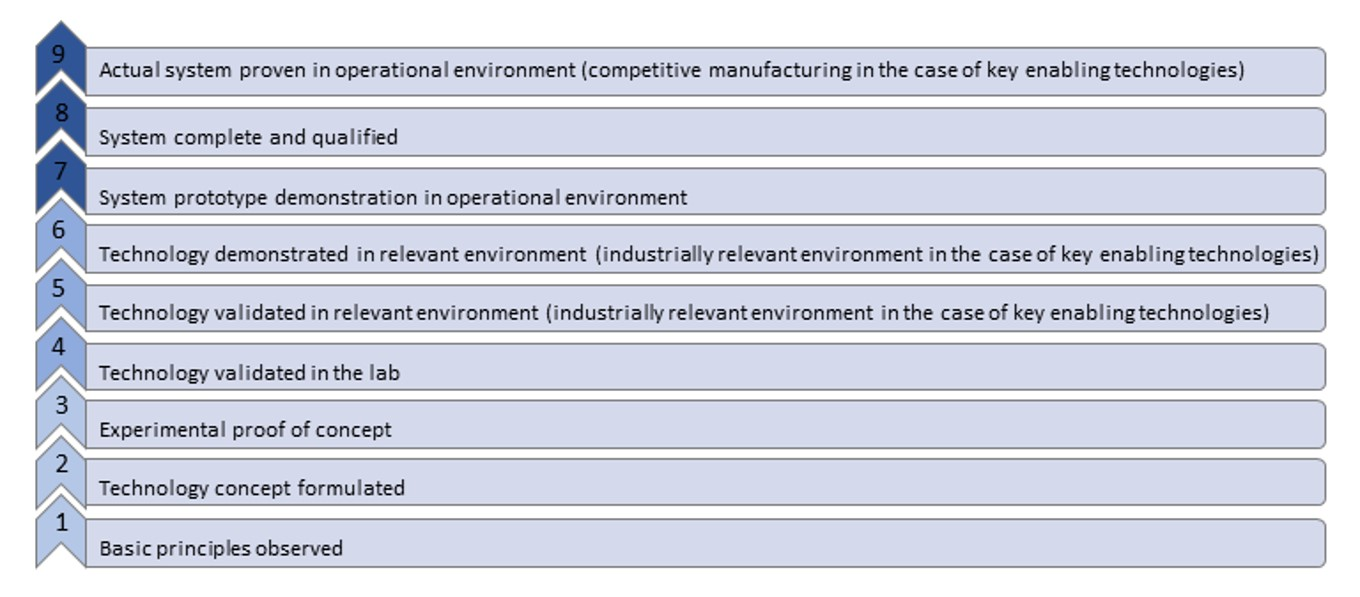
\includegraphics[width=0.8\linewidth]{image/TRL_cropped} \caption{Skala der technologischen Bereitschaft.}\label{fig:unnamed-chunk-4}
\end{figure}

Darüber hinaus bewerten wir die Bereitschaft einer bestimmten Technologie, in der Gesellschaft akzeptiert zu werden, und wie gut sie zum Gemeinwohl beiträgt, indem wir die \textbf{Skala der gesellschaftlichen Bereitschaft} verwenden (McCulloch, 2019):

\begin{figure}
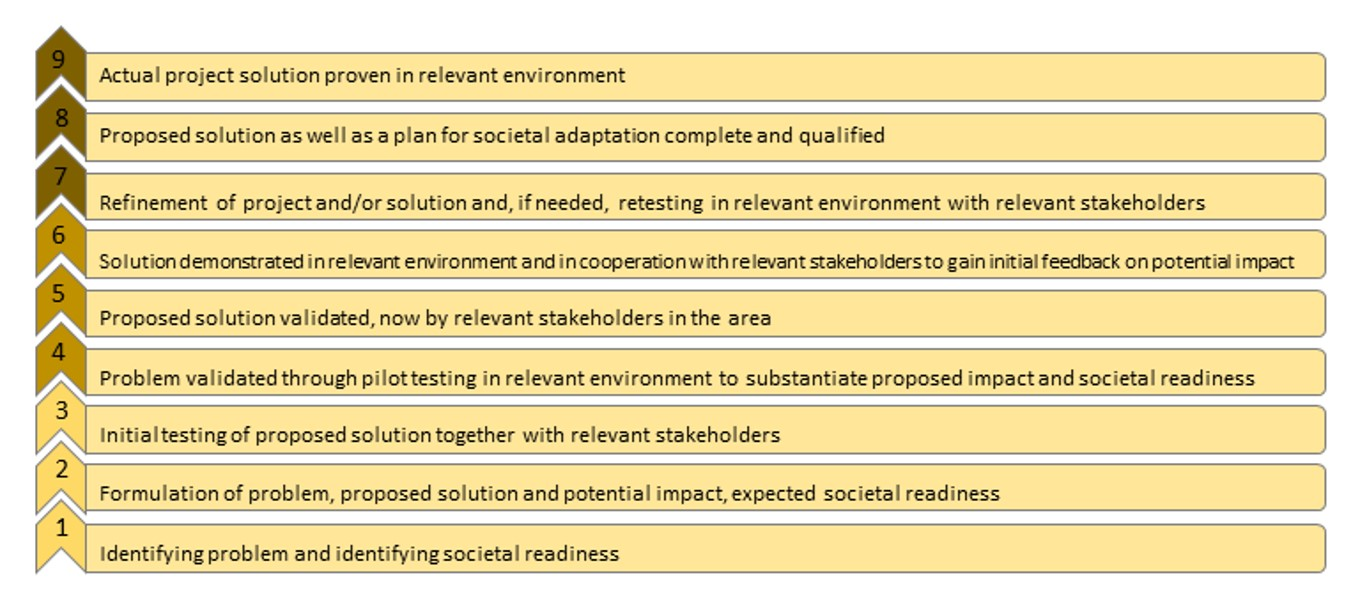
\includegraphics[width=0.8\linewidth]{image/SRL_cropped} \caption{Skala fuer die gesellschaftliche Bereitschaft.}\label{fig:unnamed-chunk-5}
\end{figure}

Abschließend finden Sie eine Liste \textbf{offener Fragen} und \textbf{Links zu weiteren Quellen} zu diesem Thema.

\textbf{Referenzen}

\begin{itemize}
\tightlist
\item
  Williamson, R., \& Beasley, J. (2011). \emph{Automotive technology and manufacturing readiness levels: a guide to recognised stages of development within the automotive industry}. URN11/672.
\item
  McCulloch, S. (2019). Social Acceptance And Societal Readiness Levels. \emph{DecarboN8}. Available at: \url{https://decarbon8.org.uk/social-acceptance-and-societal-readiness-levels/\#:~:text=Societal\%20readiness\%20refers\%20to\%20the,contributes\%20to\%20the\%20public\%20good.} {[}Accessed: 21 January 2021{]}.
\end{itemize}

\hypertarget{infrastructure}{%
\chapter{Physische Straßeninfrastruktur}\label{infrastructure}}

\hypertarget{dedicated_lanes}{%
\section{Gesonderte Fahrspuren für vernetzte und automatisierte Fahrzeuge}\label{dedicated_lanes}}

\hypertarget{synonyme}{%
\subsection*{Synonyme}\label{synonyme}}
\addcontentsline{toc}{subsection}{Synonyme}

\emph{vernetzte und automatisierte Fahrzeuge} \emph{(CAV - connected and automated vehicles)}, \emph{AV-eigene Fahrspuren} \emph{(AV-dedicated lanes)}, \emph{AV-eigene Korridore} \emph{(dedicated corridors)}

\hypertarget{definition}{%
\subsection*{Definition}\label{definition}}
\addcontentsline{toc}{subsection}{Definition}

Dedizierte Fahrspuren für vernetzte und automatisierte Fahrzeuge verfügen über zusätzliche Infrastruktur oder Sensoren, um die Zuverlässigkeit von \protect\hyperlink{adas}{fortschrittlichen Fahrerassistenzsystemen (ADAS)} zu erhöhen. Auf diesen Fahrspuren dürfen nur vollständig automatisiert fahrende Fahrzeuge fahren. Zu den typischen Anwendungen gehören kooperative und adaptive Geschwindigkeitsregelung auf der Grundlage von Sensoren mit der Infrastruktur, Spurhaltung, Optimierung des Kraftstoffverbrauchs und Möglichkeiten der Straßenbenutzung (Broek et al., 2011). Es wird erwartet, dass die Einführung von Sonderfahrspuren für CAV direkte Auswirkungen auf den Verkehrsfluss auf den Autobahnen und im nahen gelegenen Straßennetz haben wird. So zeigte eine in Singapur durchgeführte Studie, dass dedizierte Fahrspuren auf Autobahnen die Fahrzeit von CAVs um etwa 25 \% verkürzen können (wenn die Auslastung der Fahrspur nicht erreicht wird) - auf Kosten einer Verzögerung von etwa 7 \% für konventionelle Fahrzeuge aufgrund der geringeren Kapazität (Ivanchev et al., 2017). Es wurde auch nachgewiesen, dass sie sich positiv auf den Kraftstoffverbrauch auswirken.
Darüber hinaus erhöhte sich der Durchsatz, definiert als Anzahl der Fahrzeuge, die die Straße in einem bestimmten Zeitintervall passieren, infolge der Einführung von speziellen Fahrspuren für AVs (Kumar et al., 2020). Dieser Effekt war jedoch mit einem Rückgang des Durchsatzes auf kleineren Straßen verbunden, da AVs aufgrund der Zeitersparnis Autobahnen bevorzugen, was wiederum zu Zeitverlusten für konventionelle Autos führen kann. Darüber hinaus können die Vorteile einer erhöhten Kapazität von reinen AV-Fahrspuren durch die Festlegung höherer Geschwindigkeitsbegrenzungen für diese Fahrspuren noch verstärkt werden (Ye \& Yamamoto, 2018). In Bezug auf die Nachfrage nach verschiedenen Straßentypen ergab die Studie, dass die Einführung dedizierter AV-Spuren die Nachfrage konventioneller Fahrzeuge nach Hauptverkehrsstraßen (die jedoch kleiner als Autobahnen sind) und Nebenstraßen als Ersatz für stärker überlastete Autobahnen erhöhen wird.
Im Gegensatz dazu hat die Studie von Chen et al.~(2016) gezeigt, dass die Einführung von AV-Spuren das Potenzial hat, die Verkehrskapazität auf diesen Spuren in einem Mischverkehrskontext zu maximieren, während sie praktisch keine Auswirkungen auf die konventionelle Verkehrskapazität hat. Um die dedizierten Fahrspuren für CAVs effizient zu nutzen, die in der Anfangsphase möglicherweise nicht ausreichend ausgelastet sind, wird vorgeschlagen, konventionellen Fahrzeugen die Einfahrt in die reinen Fahrspuren für AVs nach Zahlung der Maut zu ermöglichen. Diese Lösung basiert auf den derzeit weltweit genutzten HOV-Spuren (High Occupancy Vehicle). Es wird behauptet, dass dieser gemeinsame Ansatz den Durchsatz auf einzelnen Straßen und die Verteilung des Verkehrsflusses im gesamten Netz verbessert (Liu \& Song, 2019).

\hypertarget{wichtige-interessensgruppen}{%
\subsection*{Wichtige Interessensgruppen}\label{wichtige-interessensgruppen}}
\addcontentsline{toc}{subsection}{Wichtige Interessensgruppen}

\begin{itemize}
\tightlist
\item
  \textbf{Betroffene}: Fahrer:innen konventioneller Autos, Autohersteller, Versicherungen
\item
  \textbf{Verantwortlich}: Straßeninfrastruktur-Agenturen, lokale und nationale Regierungen
\end{itemize}

\hypertarget{aktueller-stand-der-wissenschaft-und-forschung}{%
\subsection*{Aktueller Stand der Wissenschaft und Forschung}\label{aktueller-stand-der-wissenschaft-und-forschung}}
\addcontentsline{toc}{subsection}{Aktueller Stand der Wissenschaft und Forschung}

Die derzeitige Forschung konzentriert sich darauf, die Auswirkungen der Einführung von Standspuren auf den Verkehrsfluss, die Akzeptanz des Fahrerverhaltens, die Sicherheit und die Effizienz zu ermitteln. Darüber hinaus werden die Faktoren, die diese beeinflussen, analysiert, indem verschiedene Entwurfs- und Betriebskonfigurationen, Straßentypen und Nutzungsstrategien getestet werden (Rad et al., 2020). Es wurden sowohl Feldversuche als auch Studien an Fahrsimulatoren durchgeführt, um den Einfluss verschiedener Designs dedizierter Fahrspuren auf Fahrer:innen in konventionellen Fahrzeugen und solchen mit einem gewissen Grad an Automatisierung zu untersuchen (Guin et al., 2008, Zhong, 2018). Insbesondere wurden in einer Reihe von Studien verschiedene Arten von Fahrspuren verglichen (Zhong, 2018, Yang et al., 2019). Sie zeigten, dass Standspuren mit beschränktem Zugang in Bezug auf Fahrzeit und Durchsatz besser abschnitten als Standspuren mit durchgehendem Zugang. Darüber hinaus war die Wahrscheinlichkeit, dass Fahrzeuge in einem Zug fahren, auf separaten Fahrspuren mit begrenztem Zugang deutlich höher. Andererseits wurde gezeigt, dass die Kollisionsraten in der Nähe der Ein- oder Ausfahrt dieser Fahrspuren mit beschränktem Zugang höher sind (Rad et al.~2020).

\hypertarget{aktueller-stand-der-praktischen-umsetzung}{%
\subsection*{Aktueller Stand der praktischen Umsetzung}\label{aktueller-stand-der-praktischen-umsetzung}}
\addcontentsline{toc}{subsection}{Aktueller Stand der praktischen Umsetzung}

Derzeit plant der Bundesstaat Michigan zusammen mit mehreren privaten Partnern, darunter Ford und Alphabet Inc., 65 km einer Autobahn zwischen Detroit und Ann Arbor für den ausschließlichen Verkehr von vollständig automatisierten Fahrzeugen, einschließlich Bussen und Shuttles, zu reservieren (Krisher \& Eggert, 2020). Ähnliche Initiativen gibt es auch in anderen Ländern. So plant China den Bau einer fast 100 km langen achtspurigen Autobahn zwischen Peking und der Xiongan New Area, von der zwei Fahrspuren für den vollständig automatisierten Verkehr vorgesehen sind. Der Abschluss der Bauphase ist für Ende 2020 vorgesehen, während die Eröffnung für den Verkehr im Juni 2021 erwartet wird (Syncedreview.com, 2020). In Europa läuft derzeit das Projekt SHOW (SHared automation Operating models for Worldwide adoption), das den Einsatz von etwa siebzig vollständig automatisierten Fahrzeugen in 21 europäischen Städten vorsieht. Um zu prüfen, wie sie am besten integriert werden können, werden die Fahrzeuge in verschiedenen Umgebungen im gemischten Verkehr und auf speziellen Fahrspuren eingesetzt. Aus Sicherheitsgründen wird der Fahrer jedoch an Bord sein (CORDIS, 2020).

\hypertarget{relevante-initiativen-in-uxf6sterreich}{%
\subsection*{Relevante Initiativen in Österreich}\label{relevante-initiativen-in-uxf6sterreich}}
\addcontentsline{toc}{subsection}{Relevante Initiativen in Österreich}

\begin{itemize}
\tightlist
\item
  \href{https://www.tugraz.at/fileadmin/user_upload/Institute/IHF/Projekte/ENABLE-S3_SummaryofResults_May2019.pdf}{tugraz.at}
\item
  \href{https://www.ait.ac.at/themen/verkehrssicherheit-und-unfallforschung/projects/via-autonom/}{ait.ac.at}
\end{itemize}

\hypertarget{auswirkungen-in-bezug-auf-die-ziele-fuxfcr-nachhaltige-entwicklung-sdgs}{%
\subsection*{Auswirkungen in Bezug auf die Ziele für nachhaltige Entwicklung (SDGs)}\label{auswirkungen-in-bezug-auf-die-ziele-fuxfcr-nachhaltige-entwicklung-sdgs}}
\addcontentsline{toc}{subsection}{Auswirkungen in Bezug auf die Ziele für nachhaltige Entwicklung (SDGs)}

\begin{longtable}[]{@{}ccccc@{}}
\toprule
\begin{minipage}[b]{0.17\columnwidth}\centering
Ebene der Auswirkungen\strut
\end{minipage} & \begin{minipage}[b]{0.16\columnwidth}\centering
Indikator\strut
\end{minipage} & \begin{minipage}[b]{0.17\columnwidth}\centering
Richtung der Auswirkungen\strut
\end{minipage} & \begin{minipage}[b]{0.17\columnwidth}\centering
Beschreibung des Ziels \& SDG\strut
\end{minipage} & \begin{minipage}[b]{0.17\columnwidth}\centering
Quelle\strut
\end{minipage}\tabularnewline
\midrule
\endhead
\begin{minipage}[t]{0.17\columnwidth}\centering
Individuell\strut
\end{minipage} & \begin{minipage}[t]{0.16\columnwidth}\centering
Geringerer Kraftstoffverbrauch\strut
\end{minipage} & \begin{minipage}[t]{0.17\columnwidth}\centering
\textbf{+}\strut
\end{minipage} & \begin{minipage}[t]{0.17\columnwidth}\centering
Oekologische Nachhaltigkeit (\emph{7,12,13,15})\strut
\end{minipage} & \begin{minipage}[t]{0.17\columnwidth}\centering
Ivanchev et al., 2017\strut
\end{minipage}\tabularnewline
\begin{minipage}[t]{0.17\columnwidth}\centering
Individuell\strut
\end{minipage} & \begin{minipage}[t]{0.16\columnwidth}\centering
Verkuerzte Reisezeit\strut
\end{minipage} & \begin{minipage}[t]{0.17\columnwidth}\centering
\textbf{+}\strut
\end{minipage} & \begin{minipage}[t]{0.17\columnwidth}\centering
Nachhaltige wirtschaftliche Entwicklung (\emph{8,11})\strut
\end{minipage} & \begin{minipage}[t]{0.17\columnwidth}\centering
Zhong, 2018; Yang et al., 2019\strut
\end{minipage}\tabularnewline
\begin{minipage}[t]{0.17\columnwidth}\centering
Systemisch\strut
\end{minipage} & \begin{minipage}[t]{0.16\columnwidth}\centering
Kollisionsrate reduziert\strut
\end{minipage} & \begin{minipage}[t]{0.17\columnwidth}\centering
\textbf{+}\strut
\end{minipage} & \begin{minipage}[t]{0.17\columnwidth}\centering
Gesundheit und Wohlbefinden (\emph{3})\strut
\end{minipage} & \begin{minipage}[t]{0.17\columnwidth}\centering
Zhang et al., 2020\strut
\end{minipage}\tabularnewline
\begin{minipage}[t]{0.17\columnwidth}\centering
Systemisch\strut
\end{minipage} & \begin{minipage}[t]{0.16\columnwidth}\centering
Emissionsrate reduziert\strut
\end{minipage} & \begin{minipage}[t]{0.17\columnwidth}\centering
\textbf{+}\strut
\end{minipage} & \begin{minipage}[t]{0.17\columnwidth}\centering
Oekologische Nachhaltigkeit (\emph{7,12,13,15})\strut
\end{minipage} & \begin{minipage}[t]{0.17\columnwidth}\centering
Al Alam at al., 2010\strut
\end{minipage}\tabularnewline
\begin{minipage}[t]{0.17\columnwidth}\centering
Systemisch\strut
\end{minipage} & \begin{minipage}[t]{0.16\columnwidth}\centering
Verkehrsstaus\strut
\end{minipage} & \begin{minipage}[t]{0.17\columnwidth}\centering
\textbf{\textasciitilde{}}\strut
\end{minipage} & \begin{minipage}[t]{0.17\columnwidth}\centering
Nachhaltige wirtschaftliche Entwicklung (\emph{8,11})\strut
\end{minipage} & \begin{minipage}[t]{0.17\columnwidth}\centering
Ivanchev et al., 2017; Kumar et al., 2020\strut
\end{minipage}\tabularnewline
\begin{minipage}[t]{0.17\columnwidth}\centering
Systemisch\strut
\end{minipage} & \begin{minipage}[t]{0.16\columnwidth}\centering
Neuartige Designs getestet\strut
\end{minipage} & \begin{minipage}[t]{0.17\columnwidth}\centering
\textbf{+}\strut
\end{minipage} & \begin{minipage}[t]{0.17\columnwidth}\centering
Innovation und Infrastruktur (\emph{9})\strut
\end{minipage} & \begin{minipage}[t]{0.17\columnwidth}\centering
Guin et al., 2008; Zhong, 2018; Krisher \& Eggert, 2020\strut
\end{minipage}\tabularnewline
\begin{minipage}[t]{0.17\columnwidth}\centering
Systemisch\strut
\end{minipage} & \begin{minipage}[t]{0.16\columnwidth}\centering
SHOW EU Initiative\strut
\end{minipage} & \begin{minipage}[t]{0.17\columnwidth}\centering
\textbf{+}\strut
\end{minipage} & \begin{minipage}[t]{0.17\columnwidth}\centering
Partnerschaften und Kooperationen (\emph{17})\strut
\end{minipage} & \begin{minipage}[t]{0.17\columnwidth}\centering
CORDIS, 2020\strut
\end{minipage}\tabularnewline
\bottomrule
\end{longtable}

\hypertarget{stand-der-technologischen-und-der-gesellschaftlichen-bereitschaft}{%
\subsection*{Stand der Technologischen und der Gesellschaftlichen Bereitschaft}\label{stand-der-technologischen-und-der-gesellschaftlichen-bereitschaft}}
\addcontentsline{toc}{subsection}{Stand der Technologischen und der Gesellschaftlichen Bereitschaft}

\begin{longtable}[]{@{}cc@{}}
\toprule
Stand der Technologiebereitschaft & Gesellschaftlicher Bereitschaftsgrad\tabularnewline
\midrule
\endhead
5-6 & 1-3\tabularnewline
\bottomrule
\end{longtable}

\hypertarget{offene-fragen}{%
\subsection*{Offene Fragen}\label{offene-fragen}}
\addcontentsline{toc}{subsection}{Offene Fragen}

\begin{enumerate}
\def\labelenumi{\arabic{enumi}.}
\tightlist
\item
  Welches sind die potenziellen Vorteile von dedizierten AV-Spuren in Verbindung mit intelligenten Platooning-Strategien?
\item
  Wie und in welchem Ausmaß werden gemeinsame Konzepte von Automobilsektor, Flotte und Straßenbetreibern das Verkehrsmanagement verbessern und dynamische Verkehrsregelungen auch über Grenzen hinweg?
\item
  Was sind die Rollen und Verantwortlichkeiten der verschiedenen Akteure der physischen Infrastruktur für vernetzte und automatisierte Fahrzeuge?
\item
  Sollte das Fahrzeug mit jeder Straßeninfrastruktur zurechtkommen, und wenn nicht, welche Anforderungen können gestellt werden, um die bestehende Infrastruktur anzupassen?
\item
  Wie kann die Kontinuität zwischen diesen verschiedenen Umgebungen sichergestellt werden?
\item
  Welche Instrumente (z. B. mikro- und makroskopische Verkehrsmodellierung, Folgenabschätzung) können Städte in die Lage versetzen, die Auswirkungen vollständig automatisierter Fahrzeuge auf ihre physische Straßeninfrastruktur zu bewerten und
  die Bedürfnisse der vollständig automatisierten Fahrzeuge mit den Bedürfnissen der bestehenden Verkehrsträger (konventionelle Fahrzeuge, öffentliche Verkehrsmittel, Fußgänger:innen und Radfahrer:innen) abwägen. (ERTRAC, 2019)
\end{enumerate}

\hypertarget{weitere-links}{%
\subsection*{Weitere links}\label{weitere-links}}
\addcontentsline{toc}{subsection}{Weitere links}

\begin{itemize}
\tightlist
\item
  \href{https://knowledge-base.connectedautomateddriving.eu/wp-content/uploads/2019/12/SMART_2010-0064-study-report-final_V1-2.pdf}{knowledge base}
\item
  \href{https://show-project.eu/}{show project}
\end{itemize}

\hypertarget{referenzen}{%
\subsection*{Referenzen}\label{referenzen}}
\addcontentsline{toc}{subsection}{Referenzen}

\begin{itemize}
\tightlist
\item
  Al Alam, A., Gattami, A., \& Johansson, K. H. (2010, September). An experimental study on the fuel reduction potential of heavy duty vehicle platooning. In 13th International IEEE Conference on Intelligent Transportation Systems (pp.~306-311). IEEE.
\item
  Broek, S. M., van Nunen, E., \& Zwijnenberg, H. (2011). Definition of necessary vehicle and infrastructure systems for automated driving.
\item
  Chen, Z., He, F., Zhang, L., \& Yin, Y. (2016). Optimal deployment of autonomous vehicle lanes with endogenous market penetration. Transportation Research Part C: Emerging Technologies, 72, 143-156.
\item
  CORDIS \textbar{} European Commission. (20 Apr 2020). Available at: \url{https://cordis.europa.eu/project/id/875530} {[}Accessed: 13 November 2020{]}.
\item
  ERTRAC Working Group. (2019). Connected Automated Driving Roadmap. version, 8, 2019-08.
\item
  Guin, A., Hunter, M., \& Guensler, R. (2008). Analysis of reduction in effective capacities of high-occupancy vehicle lanes related to traffic behavior. Transportation Research Record, 2065(1), 47-53.
\item
  Ivanchev, J., Knoll, A., Zehe, D., Nair, S., \& Eckhoff, D. (2017). Potentials and implications of dedicated highway lanes for autonomous vehicles. arXiv preprint arXiv:1709.07658.
\item
  Krisher, T., \& Eggert, D. (14 Aug 2020). Michigan plans dedicated road lanes for autonomous vehicles. Available at: \url{https://abcnews.go.com/Technology/wireStory/michigan-plans-dedicated-road-lanes-autonomous-vehicles-72352758} {[}Accessed: 12 November 2020{]}.
\item
  Kumar, A., Guhathakurta, S., \& Venkatachalam, S. (2020). When and where should there be dedicated lanes under mixed traffic of automated and human-driven vehicles for system-level benefits?. Research in Transportation Business \& Management, 100527.
\item
  Liu, Z., \& Song, Z. (2019). Strategic planning of dedicated autonomous vehicle lanes and autonomous vehicle/toll lanes in transportation networks. Transportation Research Part C: Emerging Technologies, 106, 381-403.
\item
  Rad, S. R., Farah, H., Taale, H., van Arem, B., \& Hoogendoorn, S. P. (2020). Design and operation of dedicated lanes for connected and automated vehicles on motorways: A conceptual framework and research agenda. Transportation Research Part C: Emerging Technologies, 117, 102664.
\item
  Syncedreview.com (31 Aug 2020). Beijing Builds 100km Highway Lanes for Self-Driving Cars with Unmanned Machineries. Available at: \url{https://syncedreview.com/2020/08/31/beijing-builds-100km-highway-lanes-for-self-driving-cars-with-unmanned-machineries/} {[}Accessed: 12 November 2020{]}.
\item
  Yang, D., Farah, H., Schoenmakers, M. J., \& Alkim, T. (2019). Human drivers behavioural adaptation when driving next to a platoon of automated vehicles on a dedicated lane and implications on traffic flow: a driving simulator and microscopic simulation study in the Netherlands. In 98th Annual Meeting of the Transportation Research Board (pp.~19-00582).
\item
  Ye, L., \& Yamamoto, T. (2018). Impact of dedicated lanes for connected and autonomous vehicle on traffic flow throughput. Physica A: Statistical Mechanics and its Applications, 512, 588-597.
\item
  Zhang, J., Wu, K., Cheng, M., Yang, M., Cheng, Y., \& Li, S. (2020). Safety Evaluation for Connected and Autonomous Vehicles’ Exclusive Lanes considering Penetrate Ratios and Impact of Trucks Using Surrogate Safety Measures. Journal of advanced transportation, 2020.
\item
  Zhong, Z. (2018). Assessing the effectiveness of managed lane strategies for the rapid deployment of cooperative adaptive cruise control technology.
\end{itemize}

\hypertarget{ODD}{%
\section{Operative Gestaltungsbereiche (Operational design domains)}\label{ODD}}

\hypertarget{synonyme-1}{%
\subsection*{Synonyme}\label{synonyme-1}}
\addcontentsline{toc}{subsection}{Synonyme}

\emph{ODD}

\hypertarget{definition-1}{%
\subsection*{Definition}\label{definition-1}}
\addcontentsline{toc}{subsection}{Definition}

Operational Design Domain (ODD) ist ein System zur Bewertung der Bedingungen, unter denen ein automatisiertes Fahrsystem (automated driving system - ADS) auf der Grundlage von Fahrbahnmerkmalen oder des Verkehrsaufkommens sicher arbeiten kann (Czarnecki, 2018). Es ist ein Schlüssel zur Sicherheit von automatisierten Fahrzeugen, und ODD ist dazu da, die Grenzen für das Fahren auf verschiedenen Automatisierungsstufen eines Fahrzeugs zu definieren (Eliot, 2019). Zum Beispiel hat die Automatisierungsstufe 5 eine uneingeschränkte ODD, was bedeutet, dass sie der Steuerung des Fahrzeugs durch einen menschlichen Fahrer:innen gleichkommt. Bei den Stufen 1-4 unterliegt die ODD Beschränkungen in Bezug auf (Czarnecki, 2018):

\begin{itemize}
\tightlist
\item
  Straßenumgebung: einschließlich, aber nicht beschränkt auf städtische und ländliche Straßen, Autobahnen, Kreisverkehre, Tunnel, Verkehrsaufkommen, Baustellen oder unterschiedliche Wetter- oder Sichtbedingungen
\item
  Zustand des Fahrzeugs: z. B. Beladungsgrenzen oder Mindestfüllstand der Reifen
\item
  Verhalten des mit ADS ausgerüsteten Fahrzeugs: z. B. Geschwindigkeitsbegrenzungen oder Beschränkungen für mögliche Fahrmanöver
\end{itemize}

Im Allgemeinen bewertet ODD die Bedingungen, ob das Fahrzeug in der Lage ist, auf der gewählten Strecke und dem gegebenen Automatisierungsgrad automatisiert zu fahren. Stellt das System irgendwann fest, dass die Bedingungen für automatisiertes Fahren nicht geeignet sind, findet ODD einfach eine Stelle, an der das Fahrzeug angehalten werden kann, und Fahrer:innen müssen selbst das Steuer übernehmen und losfahren.

Der ODD arbeitet auf der Grundlage des operationellen Weltmodells (OWM), das aus dem operationellen Straßenumgebungsmodell \emph{(operational road environment model - OREM)}, dem Modell des betreffenden Fahrzeugs \emph{(subject vehicle(s) model - SVM)} und dem \emph{ADS} besteht. OREM repräsentiert alle relevanten Annahmen über die Straßenumgebung, in der ein ADS betrieben wird, während die irrelevanten ignoriert werden. SVM repräsentiert ein Fahrzeug, das von dem entwickelten ADS betrieben wird. Das OMW kann ein einzelnes Fahrzeug oder mehrere Fahrzeuge umfassen, die mit demselben oder verschiedenen ADS ausgestattet sind. Die Einbeziehung verschiedener ADS kann notwendig sein, um die Interaktion zwischen verschiedenen Fahrzeugtypen wie Bussen und Personenkraftwagen oder denselben Fahrzeugtypen mit unterschiedlichem ADS-Entwicklungsstand darzustellen.

Darüber hinaus führen Koopman und Fratrik (2019) eine Liste von Faktoren an, die für die Validierung und den Betrieb automatisierter Fahrzeuge und folglich für die Entwicklung von ODD als relevant erachtet werden. Dazu gehören:

\begin{itemize}
\tightlist
\item
  Betriebliches Terrain
\item
  Wetterbedingungen
\item
  Betriebliche Infrastruktur
\item
  Einsatzregeln und Interaktion mit der Umgebung und anderen Verkehrsteilnehmer:innen
\item
  Überlegungen zum Einsatz in mehreren Regionen
\item
  Datenverfügbarkeit und Aktualität (z. B. in Bezug auf vorübergehende Änderungen der Verkehrsregeln)
\item
  Erwartete Elemente des operativen Raumzustands (z. B. was sollte in den Anwendungsbereich von ODD einbezogen werden)
\end{itemize}

Darüber hinaus bezieht sich Object and Event Detection and Response (OEDR) auf den Betrieb innerhalb des Geltungsbereichs einer definierten ODD in Bezug auf Objekte und Ereignisse. Zu den \emph{Objektfaktoren} gehören:

\begin{itemize}
\tightlist
\item
  Fähigkeit, relevante Objekte in der Umgebung zu erkennen und zu klassifizieren
\item
  Verarbeitung und Schwellenwertbildung von Sensordaten
\item
  Charakterisierung möglicher Betriebsparameter anderer Verkehrsteilnehmer:innen
\item
  Permanente (Bäume, Bordsteine usw.) und temporäre (z. B. Menschen, Überschwemmungen) Hindernisse
\item
  Gefährdete Bevölkerung
\item
  Alle Arten von anderen Verkehrsteilnehmer:innen, einschließlich von Menschen gesteuerter und automatisierter Fahrzeuge sowie von Spezialfahrzeugen und Flugzeugen
\end{itemize}

Darüber hinaus beziehen sich die \emph{Ereignisfaktoren} auf:
- Bestimmung des Verhaltens anderer Objekte
- `Normale' Bewegung von Objekten
- `Anormale' Bewegung von Objekten
- Ausbleiben der Bewegung anderer Objekte
- Interaktionen des/der Fahrer:in vor, während und nach dem Einsatz des automatisierten Systems
- Menschliche und nicht-menschliche Interaktionen

\hypertarget{wichtige-interessensgruppen-1}{%
\subsection*{Wichtige Interessensgruppen}\label{wichtige-interessensgruppen-1}}
\addcontentsline{toc}{subsection}{Wichtige Interessensgruppen}

\begin{itemize}
\tightlist
\item
  \textbf{Betroffene}: Fahrer:innen konventioneller Autos, Autohersteller, Nutzer:innen von AVs
\item
  \textbf{Verantwortlich}: Stadtverwaltungen, Autohersteller, Versicherungsanbieter
\end{itemize}

\hypertarget{aktueller-stand-der-wissenschaft-und-forschung-1}{%
\subsection*{Aktueller Stand der Wissenschaft und Forschung}\label{aktueller-stand-der-wissenschaft-und-forschung-1}}
\addcontentsline{toc}{subsection}{Aktueller Stand der Wissenschaft und Forschung}

Die aktuelle Forschung konzentriert sich auf die Validierung, die Erweiterung der Fähigkeiten und die Verbesserung der Genauigkeit der derzeitigen ODD-Systeme. Lee et al.~(2020) schlagen beispielsweise einen Ansatz zur Ermittlung einer ODD für das ADS anhand von statistischen Daten und Risikotoleranz vor. Die ermittelte ODD basiert auf der geografischen Zuordnung des mit dem ADS-Betrieb verbundenen Risikoniveaus, das unter der für eine bestimmte Umweltbedingung vordefinierten Risikoschwelle liegt. Daher ermöglicht diese Methode die Berücksichtigung von Sicherheitsbedenken durch die Festlegung von geografischen und umweltbedingten Einschränkungen für den ADS-Betrieb. Darüber hinaus untersuchten Farah et al.~(2020) das Verständnis von ODD (in Bezug auf das Halten der Fahrspur) durch menschliche Fahrer:innen, von denen erwartet wird, dass sie das Fahrzeug in Situationen außerhalb der vom Hersteller angegebenen ODD steuern. Ein Unterschied zwischen dem Verständnis der Fahrer:innen für die Fähigkeiten des AV und dem Handbuch des Herstellers kann zu ernsthaften Sicherheitsproblemen führen. Sie führten einen Feldtest mit einem Tesla Model S durch, der auf Situationen innerhalb und außerhalb der vom Hersteller angegebenen ODD basierte. Farah et al.~(2020) fanden eine Diskrepanz zwischen der vom Hersteller angegebenen ODD und der Wahrnehmung der Fahrer:innen, was die ODD umfasst. Insbesondere wurden Situationen, die außerhalb des Geltungsbereichs der ODD lagen, von menschlichen Fahrer:innen häufig als innerhalb des ODD-Bereichs liegend eingestuft. Diese Studie hat gezeigt, dass die ODD klarer beschrieben und spezifiziert werden muss, um die Diskrepanz zwischen dem Bewusstsein der Fahrer:innen und den tatsächlichen Fähigkeiten des Fahrzeugs zu verringern.

\hypertarget{aktueller-stand-der-praktischen-umsetzung-1}{%
\subsection*{Aktueller Stand der praktischen Umsetzung}\label{aktueller-stand-der-praktischen-umsetzung-1}}
\addcontentsline{toc}{subsection}{Aktueller Stand der praktischen Umsetzung}

Kalifornien ist einer der Pionierstaaten, die Versuche zur Erprobung von ODD durchführen. Eines der Beispiele ist das aktuelle Google-Projekt des fahrerlosen Testwagens von Waymo \href{https://www.losaltoshills.ca.gov/DocumentCenter/View/2315/Waymo_Driverless_Autonomous_Vehicle_Tester_Program}{Waymo’s}. Es verwendet eine vierte Stufe des automatisierten Fahrsystems und zeigt die Verwendung von ODD im wirklichen Leben. Das ODD von Waymo arbeitet in einem bestimmten geografischen Gebiet (einem Teil Kaliforniens) 24 Stunden am Tag. Waymos ODD kann bis zu 105 km/h erreichen, funktioniert aber nicht bei Schnee oder Regen. Ansonsten gibt es in den USA keine landesweite Regelung für den Einsatz von ODD, da diese sehr ortsabhängig sind. Andere Regionen der Welt arbeiten an eigenen Regelungen für ODDs, wie z. B. MLIT-Guidline in Japan, Transport Canada in Kanada, NHTSA FAVP 3.0 in den USA oder EG-Richtlinien in Europa. Darüber hinaus hat die informelle Arbeitsgruppe der Vereinten Nationen für funktionale Anforderungen für AVs (FRAV) einen {[}Bericht{]} (\url{https://unece.org/fileadmin/DAM/trans/doc/2020/wp29grva/GRVA-05-40e.pdf}) zur Regelung der funktionalen Leistungsanforderungen für automatisierte Fahrsysteme und mit solchen Systemen ausgestattete Fahrzeuge vorgelegt.

\hypertarget{relevante-initiativen-in-uxf6sterreich-1}{%
\subsection*{Relevante Initiativen in Österreich}\label{relevante-initiativen-in-uxf6sterreich-1}}
\addcontentsline{toc}{subsection}{Relevante Initiativen in Österreich}

\begin{itemize}
\tightlist
\item
  \href{https://austriatech.at/de/das-konzept-der-isad-klassen/}{AustriaTech}
\end{itemize}

\hypertarget{auswirkungen-in-bezug-auf-die-ziele-fuxfcr-nachhaltige-entwicklung-sdgs-1}{%
\subsection*{Auswirkungen in Bezug auf die Ziele für nachhaltige Entwicklung (SDGs}\label{auswirkungen-in-bezug-auf-die-ziele-fuxfcr-nachhaltige-entwicklung-sdgs-1}}
\addcontentsline{toc}{subsection}{Auswirkungen in Bezug auf die Ziele für nachhaltige Entwicklung (SDGs}

\begin{longtable}[]{@{}ccccc@{}}
\toprule
\begin{minipage}[b]{0.17\columnwidth}\centering
Ebene der Auswirkungen\strut
\end{minipage} & \begin{minipage}[b]{0.16\columnwidth}\centering
Indikator\strut
\end{minipage} & \begin{minipage}[b]{0.17\columnwidth}\centering
Richtung der Auswirkungen\strut
\end{minipage} & \begin{minipage}[b]{0.17\columnwidth}\centering
Beschreibung des Ziels \& SDG\strut
\end{minipage} & \begin{minipage}[b]{0.17\columnwidth}\centering
Quelle\strut
\end{minipage}\tabularnewline
\midrule
\endhead
\begin{minipage}[t]{0.17\columnwidth}\centering
Systemisch\strut
\end{minipage} & \begin{minipage}[t]{0.16\columnwidth}\centering
Mehr Sicherheit fuer automatisierte Fahrzeuge angestrebt\strut
\end{minipage} & \begin{minipage}[t]{0.17\columnwidth}\centering
\textbf{+}\strut
\end{minipage} & \begin{minipage}[t]{0.17\columnwidth}\centering
Gesundheit und Wohlbefinden (\emph{3})\strut
\end{minipage} & \begin{minipage}[t]{0.17\columnwidth}\centering
Koopman and Fratrik, 2019\strut
\end{minipage}\tabularnewline
\begin{minipage}[t]{0.17\columnwidth}\centering
Systemisch\strut
\end{minipage} & \begin{minipage}[t]{0.16\columnwidth}\centering
Entwicklung vollstaendig automatisierter Autos\strut
\end{minipage} & \begin{minipage}[t]{0.17\columnwidth}\centering
\textbf{+}\strut
\end{minipage} & \begin{minipage}[t]{0.17\columnwidth}\centering
Innovation und Infrastruktur (\emph{9})\strut
\end{minipage} & \begin{minipage}[t]{0.17\columnwidth}\centering
Waymo, 2019\strut
\end{minipage}\tabularnewline
\bottomrule
\end{longtable}

\hypertarget{stand-der-technologiebereitschaft-und-gesellschaftlicher-bereitschaftsgrad}{%
\subsection*{Stand der Technologiebereitschaft und Gesellschaftlicher Bereitschaftsgrad}\label{stand-der-technologiebereitschaft-und-gesellschaftlicher-bereitschaftsgrad}}
\addcontentsline{toc}{subsection}{Stand der Technologiebereitschaft und Gesellschaftlicher Bereitschaftsgrad}

\begin{longtable}[]{@{}cc@{}}
\toprule
TRL & SRL\tabularnewline
\midrule
\endhead
5-6 & 4-6\tabularnewline
\bottomrule
\end{longtable}

\hypertarget{offene-fragen-1}{%
\subsection*{Offene Fragen}\label{offene-fragen-1}}
\addcontentsline{toc}{subsection}{Offene Fragen}

\begin{enumerate}
\def\labelenumi{\arabic{enumi}.}
\tightlist
\item
  Welchen Einfluss hat die Entwicklung von ODD auf den Markt für automatisierte Fahrzeuge für den Durchschnittsfahrer?
\end{enumerate}

\hypertarget{referenzen-1}{%
\subsection*{Referenzen}\label{referenzen-1}}
\addcontentsline{toc}{subsection}{Referenzen}

\begin{itemize}
\tightlist
\item
  Berman, B., 2019. Autonomous vehicle operation design domain is key to safety. Sae.org. Available at: \url{https://www.sae.org/news/2019/11/odds-for-av-testing} {[}Accessed: 2 August 2021{]}.
\item
  Czarnecki, K. (2018). Operational Design Domain for Automated Driving Systems - Taxonomy of Basic Terms. 10.13140/RG.2.2.18037.88803.
\item
  Eliot, L., 2019. Key To Driverless Cars, Operational Design Domains (ODD), Here’s What They Are, Woes Too. Medium. Available at: \url{https://lance-eliot.medium.com/key-to-driverless-cars-operational-design-domains-odd-heres-what-they-are-woes-too-a0f1059e0bdb} {[}Accessed: 2 August 2021{]}.
\item
  Farah, H., Bhusari, S., Van Gent, P., Babu, F. A. M., Morsink, P., Happee, R., \& van Arem, B. (2020). An empirical analysis to assess the operational design domain of lane keeping system equipped vehicles combining objective and subjective risk measures. IEEE Transactions on Intelligent Transportation Systems, 22(5), 2589-2598.
\item
  Koopman, P. and Fratrik, F., (2019). How Many Operational Design Domains, Objects, and Events?. Ceur-ws.org. Available at: \url{http://ceur-ws.org/Vol-2301/paper_6.pdf} {[}Accessed: 2 August 2021{]}.
\item
  Law Insider. (2021). Operational design domain Definition \textbar{} Law Insider. Available at: \url{https://www.lawinsider.com/dictionary/operational-design-domain} {[}Accessed: 2 August 2021{]}.
\item
  Lee, C., Nayeer, N., Garcia, D., Agrawal, A. and Liu, B., 2020. Identifying the Operational Design Domain for an Automated Driving System through Assessed Risk. 2020 IEEE Intelligent Vehicles Symposium (IV).
\item
  Waymo. 2019. Waymo. Available at: \url{https://waymo.com/} {[}Accessed: 2 August 2021{]}.
\end{itemize}

\hypertarget{rail_crossing_info_system}{%
\section{Informationssystem für Bahnübergänge}\label{rail_crossing_info_system}}

\hypertarget{synonyme-2}{%
\subsection*{Synonyme}\label{synonyme-2}}
\addcontentsline{toc}{subsection}{Synonyme}

\emph{Bahnübergänge (rail level crossings - RLX), erhöhte Bahnübergänge (raised level crossings - RC), Bahnübergangshinderniserkennung (Level Crossing Obstacle Detection - LOD), Bahnübergang (level crossing - LC)}

\hypertarget{definition-2}{%
\subsection*{Definition}\label{definition-2}}
\addcontentsline{toc}{subsection}{Definition}

Ein anhaltendes Problem im Landverkehr sind Kollisionen an Bahnübergängen (RLX). RLX sind höhengetrennte Kreuzungen, an denen Schienenfahrzeuge (und ihre Infrastruktur) die Infrastruktur eines anderen Verkehrsträgers (in der Regel Straßen) kreuzen. In den meisten Fällen hat der Zug Vorrang und der übrige Verkehr wird angehalten, bis der Zug vorbeigefahren ist. Technisch gesehen ist diese Entflechtung ein einfaches Problem (Salmon et al., 2016). Dennoch kommt es jedes Jahr zu einer Reihe von Unfällen.
Kollisionen an Bahnübergängen stellen weltweit ein Sicherheitsrisiko dar (European Railway Agency, 2020). Unfälle verursachen menschliche, soziale und wirtschaftliche Kosten. Darüber hinaus wirken sich Beinahe-Kollisionen negativ auf die psychische Gesundheit und das Wohlbefinden der beteiligten Personen -- Autofahrer:innen, Zugführer:innen und Umstehende - aus (Read et al., 2021). Die beste Möglichkeit, diese Art von Unfällen zu minimieren, wäre die Beseitigung der Bahnübergänge und/oder deren Ersatz durch Tunnel oder Brücken. Da diese Optionen sehr kostspielig sind, wird für die meisten Bahnübergänge die billigere Alternative von Schildern, Blinklichtern und Schranken verwendet, in der Erwartung, dass sich die Fahrer:innen von Straßenfahrzeugen an die Regeln halten werden. Daten aus Australien zeigen jedoch, dass der größte Teil der Kollisionen an Kreuzungen mit Schranken stattfindet, während der größte Teil der tödlichen Unfälle an Kreuzungen mit Blinklicht und Stoppschildern passiert (ITSR, 2011).
Radalj et al.~(2011) haben in einer umfangreichen Feldstudie in sieben ländlichen Gemeinden nachgewiesen, dass 90 \% der Verkehrsteilnehmer:innen die Geschwindigkeitsbegrenzungen an den Signalen missachteten und dass 90 \% der Unfälle an Bahnübergängen auf Fehler der Fahrzeugführer:innen, Müdigkeit, Geschwindigkeit oder Risikobereitschaft aufgrund der geringen Zugfrequenz zurückzuführen waren. Auch in Österreich gibt es bereits Daten, die zeigen, dass praktisch alle Unfälle an Bahnübergängen von Verkehrsteilnehmer:innenn verursacht werden, die rote Ampeln, Stoppschilder, Schranken und grundlegende Verkehrsregeln nicht beachten. Sehr oft sind Menschen, die in der Nähe eines Bahnübergangs wohnen oder ihn regelmäßig überqueren, in diese Unfälle verwickelt, weil sie mit der Zeit unvorsichtiger und übermütiger werden (bmvit, 2011).
Gemäß der Europäischen Union (2014) werden Bahnübergänge in aktive und passive unterteilt:

\begin{itemize}
\tightlist
\item
  \textbf{Ein passiver Bahnübergang } ist ein Bahnübergang ohne jede Form von Warnsystem oder Schutz, der aktiviert wird, wenn es für Benutzer:innen unsicher ist, ihn zu überqueren.
\item
  \textbf{Ein aktiver Bahnübergang } ist ein Bahnübergang, bei dem die Benutzer:innen des Bahnübergangs vor einem herannahenden Zug geschützt oder gewarnt werden. Der Schutz wird durch Halb- oder Vollschranken gewährleistet. Die Warnung erfolgt durch sichtbare (z. B. Lichter) und akustische Vorrichtungen (z. B. Glocken, Hupen, Schallsignale).
\end{itemize}

Aktive Bahnübergänge werden klassifiziert als:
- \textbf{Manuell}: ein Bahnübergang, bei dem die benutzerseitige Sicherung oder Warnung manuell von Bahnmitarbeiter:innen aktiviert wird.
- \textbf{Automatisch mit benutzerseitiger Warnung: }: Ein Bahnübergang, bei dem die benutzerseitige Warnung durch den herannahenden Zug aktiviert wird.
- \textbf{Automatisch mit benutzerseitigem Schutz}: Ein Bahnübergang, bei dem der benutzerseitige Schutz durch den herannahenden Zug aktiviert wird. Dazu gehört auch ein Bahnübergang, der sowohl über einen benutzerseitigen Schutz als auch über eine Warnung verfügt.
- \textbf{Gleisseitiger Schutz}: Ein Bahnübergang, bei dem ein Signal oder ein anderes Zugsicherungssystem die Weiterfahrt eines Zuges nur dann zulässt, wenn der Bahnübergang frei von Hindernissen ist.

Die streckenseitige Sicherung ermöglicht die Erkennung von Hindernissen an Bahnübergängen durch eine oder mehrere Erfassungseinheiten, je nach Größe des Bahnübergangs. Eine streckenseitige Steuereinheit sammelt die von den Erfassungseinheiten empfangenen Informationen und erzeugt Alarme auf der Grundlage hoher Schwellenwerte (z. B. Mindestabmessungen des Hindernisses). Die Steuereinheit ist in der Lage, die Bahnübergangshinderniserkennung (BÜH) in die konventionelle Bahnübergangssicherung mit kompletten Schranken und Antrieben zu integrieren und über gesicherte Schnittstellen mit dem Stellwerk zu kommunizieren. Die Systeme zeichnen sich durch hohe Zuverlässigkeit und hohe Genauigkeit aus, auch bei rauen Wetterbedingungen wie Regen, Schnee und Nebel. Derzeit laufen mehrere Versuche mit europäischen Bahnen (mermecgroup, n.d.).

Laut Darlington (2017) muss ein ideales Hinderniserkennungssystem:

\begin{itemize}
\tightlist
\item
  eine Sicherheitsintegrität bieten, die nicht schlechter und idealerweise besser ist als bei einem manuell betriebenen Bahnübergang
\item
  keine oder nur minimale Verspätungen von Zügen aufgrund von Geräteausfällen oder Fehldetektionen verursachen
\item
  in Bezug auf die Lebenszykluskosten erschwinglich sein
\item
  bei allen Wetterbedingungen und Temperaturen funktionieren
\item
  praktisch zu bedienen und zu warten sein
\end{itemize}

Darüber hinaus müssen getrennte technische Systeme bestätigen, dass der Bahnübergang durch Schranken oder Tore geschlossen ist, und erst wenn das Detektionssystem bestätigt hat, dass der Bahnübergang frei ist, wird der Zug durchgelassen. Dies könnte durch die Freigabe der Schutzsignale oder, auf einigen Schienennetzen, durch eine direkte Kommunikationsverbindung zum Zug erreicht werden. Einige Systeme bieten zwar gute Sicherheitsvorteile, aber nur auf Kosten erheblicher betrieblicher Verzögerungen. Das Hinderniserkennungssystem muss sich in die bestehende Eisenbahninfrastruktur einfügen und soll den Betrieb nicht beeinträchtigen.
Für die Hinderniserkennung stehen folgende Technologien zur Verfügung, die jedoch alle Vor- und Nachteile haben (Darlington, 2017):

\textbf{Videobildtechnik}
Der Nachteil der Videotechnik besteht darin, dass das System bei Nacht oder Nebel nur schwer etwas erkennen kann. Der Bahnübergang benötigt daher möglicherweise die gleiche oder eine höhere Beleuchtungsstärke als ein manueller Bahnübergang, obwohl dies bei Nebel wenig hilfreich wäre. Außerdem lassen sich die Masse oder die Materialeigenschaften eines Objekts nicht so leicht unterscheiden. So könnte beispielsweise ein Karton oder eine Zeitung fälschlicherweise für ein kleines Kind gehalten werden.

\textbf{Wärmebildtechnik}
Wärmebildkameras können einige dieser Einschränkungen überwinden, da sie auf der Grundlage feiner Temperaturunterschiede ein scharfes Bild erzeugen und nicht durch Umgebungsbedingungen wie völlige Dunkelheit, Rauch oder Nebel beeinträchtigt werden. Sie benötigen kein Licht und können nicht durch direktes Sonnenlicht geblendet werden. Allerdings könnten Objekte ohne Wärmequelle an einer Kreuzung zurückgelassen werden (z. B. ein ungebremster Anhänger) und somit nicht erkannt werden. Die Wärmebildtechnik kann in Kombination mit anderen Erkennungstechnologien eine Lösung bieten.

\textbf{Strahlunterbrechung im Millimeterwellenbereich}
Die Strahlunterbrechung ist eine auf Mikrowellen basierende Technik zur Hinderniserkennung. Wenn ein Objekt in den Strahlengang eindringt, wird das Signal zum Sende-Empfangsgerät abgeschwächt, was die Anwesenheit des Objekts anzeigt. Eines der weltweit ersten Systeme der Sicherheitsintegritätsstufe (SIL) 4 wurde in Italien installiert. Obwohl das System sicher war, reagierte es sehr empfindlich auf Temperaturschwankungen, Regen und Kondenswasser auf den Sensoren von Sender und Empfänger. Es musste regelmäßig kalibriert und gewartet werden. Außerdem bedeuteten die geringe Strahlbreite und das begrenzte Sichtfeld, dass für hohe Objekte noch mehr Sensoren benötigt wurden.

\textbf{LiDAR}
LiDAR erfasst den Kreuzungsbereich mit Impulsen aus Nahinfrarotlicht, die von der Oberfläche eines Objekts auf dem Bahnübergang reflektiert werden. Die reflektierten Impulse können dann analysiert werden, um seine Position, Richtung und Geschwindigkeit zu bestimmen. Da Licht eine kürzere Wellenlänge als Radiowellen hat, bietet LiDAR das Potenzial für eine höhere Genauigkeit als Radar. Network Rail hat LiDAR bei seiner ersten Generation von OD-Kreuzungen als Ergänzung zum Radar eingesetzt, um die Erkennung von Objekten in niedriger Höhe zu verbessern. Die verbesserte Empfindlichkeit bedeutet jedoch auch, dass das System anfällig für kleine Objekte ist, wie z. B. Wasserdampftröpfchen, aus denen sich Nebel zusammensetzt, obwohl dies durch Softwarealgorithmen abgemildert werden kann. Außerdem wird für den Betrieb Licht benötigt, und die Geräte müssen in einem transparenten Gehäuse untergebracht werden, was zu einer erhöhten Anfälligkeit für Wasser, Schmutz und Staub auf dem Glas führt.

\textbf{Induktionsschleifen}
Eine Induktionsschleife wird zur Erkennung von Metallobjekten verwendet und eignet sich daher nicht für die Erkennung von Fußgänger:innen. Leider gibt es immer mehr Straßenfahrzeuge aus Verbundwerkstoffen und Aluminium, die einen geringeren induzierten Strom liefern als Stahl, und es wurde über Probleme bei der Erkennung von Lastwagen mit hohen Achsen/Bodenfreiheit berichtet. Eine weitere Schwierigkeit ist die Installation und Wartung von Induktionsschleifen in der Oberfläche der Kreuzung oder Straße.

\textbf{Dehnungsmessstreifen}
Mit einem Dehnungsmessstreifen oder Piezometer kann die Verformung (Dehnung) eines Materials gemessen werden (die Verformung der Oberfläche des Bahnübergangs, wenn ein Objekt den Bahnübergang überquert). Ein Dehnungsmessstreifen sollte sowohl für Fahrzeuge als auch für Fußgänger:innen kalibriert werden können, ist aber möglicherweise nicht in der Lage, kleine Kinder zu erkennen. Piezometer und Dehnungsmessstreifen sind potenziell zuverlässiger als Induktionsschleifen, aber durch die Platzierung der Detektoren in der Fahrbahn des Bahnübergangs sind sie genauso schwierig zu warten.

\textbf{Ultraschall-Sensoren}
Diese senden Ultraschallimpulse aus, die vom menschlichen Ohr nicht wahrgenommen werden können. Wenn der Impuls ein Objekt erreicht, wird der Schall von der Oberfläche reflektiert. Es wären mehrere Sensoren erforderlich, um schwarze Flecken zu vermeiden, und auf elektrifizierten Strecken würden sich die Geräte in unmittelbarer Nähe von Teilen der Freileitungen befinden. Die Geräte wären anfälliger für Vandalismus und Beschädigungen durch die Öffentlichkeit, da sie an einem Bahnübergang viel auffälliger sind als andere Formen der Detektion. Es wird jedoch berichtet, dass in den USA erfolgreiche Versuche zur Hinderniserkennung mit einer Reihe von Ultraschallsensoren durchgeführt wurden, die über einem Bahnübergang aufgehängt waren.

\textbf{Radar}
Es nutzt Radiowellen, um Objekte zu erkennen. Entfernung, Position und Geschwindigkeit eines Objekts können bestimmt werden. An den Grenzen des Bahnübergangs können Reflektoren installiert werden, die ein Referenz-Echosignal liefern und dieses zur Überwachung des Zustands des Bereichs und des Sensors selbst nutzen. Radargestützte Systeme sind in der Lage, Objekte auch bei Regen, Nebel, Schnee und Hagel zuverlässig zu erkennen. Es wurden OD-Radarsysteme mit SIL 4-Integrität und Systeme mit breiter Strahlbreite entwickelt, so dass für hohe und niedrige Hindernisse nicht mehrere Sensoren erforderlich sind. Ein Vorteil des Radars gegenüber anderen Erkennungsmethoden ist, dass einige materielle Objekte mit geringer Dichte, wie z. B. eine leere Pappschachtel, ignoriert werden. Da es sich um ein funkbasiertes System handelt, ist für ein Radar-OD-System normalerweise eine Funklizenz erforderlich, was jedoch bedeutet, dass der Betreiber der Eisenbahninfrastruktur die Frequenz exklusiv nutzen kann und in der Lage ist, etwaige Störungen zu bewältigen. Der Sensor ist in der Lage, unter allen Wetterbedingungen zu arbeiten, und hat eine prognostizierte mittlere Betriebsdauer zwischen Ausfällen (MTBF) von mehr als 10 Jahren.

Ein OD-System kann einen oder mehrere der verschiedenen Detektionstypen verwenden, z. B. verwenden die OD-Kreuzungen der ersten Generation von Network Rail sowohl Radar als auch Laser Image Detection and Ranging (LiDAR).

\hypertarget{wichtige-interessensgruppen-2}{%
\subsection*{Wichtige Interessensgruppen}\label{wichtige-interessensgruppen-2}}
\addcontentsline{toc}{subsection}{Wichtige Interessensgruppen}

\begin{itemize}
\tightlist
\item
  \textbf{Betroffene}: Autofahrer:innen, Radfahrer:innen, Fußgänger:innen, Zugreisende, Zugbetreiber:innen, Triebfahrzeugführer:innen
\item
  \textbf{Verantwortlich}: Nationale Regierungen, Stadtverwaltungen, Verkehrsbehörden, Eisenbahnunternehmen, Hersteller von Eisenbahnausrüstung und -infrastruktur
\end{itemize}

\hypertarget{aktueller-stand-der-wissenschaft-und-forschung-2}{%
\subsection*{Aktueller Stand der Wissenschaft und Forschung}\label{aktueller-stand-der-wissenschaft-und-forschung-2}}
\addcontentsline{toc}{subsection}{Aktueller Stand der Wissenschaft und Forschung}

Eine Fahrsimulationsstudie (Larue et al., 2015) zeigte, dass sich das Fahrerverhalten bei passiven Kreuzungen durch assistive IVS-Eingriffe änderte, während bei aktiven Kreuzungen selbst bei eingeschränkter Sicht keine Unterschiede festgestellt wurden. Die akustische Intervention führte zu einer höheren Einhaltung im Vergleich zur visuellen Intervention. Die Ergebnisse der straßengestützten IVS-Technologie deuten darauf hin, dass es unwahrscheinlich ist, dass dies zu positiven Sicherheitsergebnissen an passiven Bahnübergängen führt, wenn die Fahrer:innen weiterhin unter allen Bedingungen am Bahnübergang anhalten müssen (aufgrund des Stoppschilds am Bahnübergang). Eine akustische Intervention im Fahrzeug dürfte sich positiv auf die Sicherheit auswirken, da der Mensch in der Lage ist, Geräusche unabhängig von der Richtung zu hören, aus der das Geräusch kommt. Dies macht den Ton zu einem besonders nützlichen Medium für die Übermittlung von sicherheitskritischen Meldungen.
Viele Autor:innen untersuchen das Fahrerverhalten an Bahnübergängen (Beanland et al., 2017; Hao et al., 2015; Larue et al., 2015; Tey et al., 2013). Eine systematische Studie von Read et al.~(2021) kategorisiert die Faktoren, die das Risiko an Bahnübergängen beeinflussen, nach 3 Aspekten:

\begin{itemize}
\item
  Unfallhäufigkeit und -schwere
\item
  unsicheres und nicht konformes Verhalten der Verkehrsteilnehmer:innen
\item
  Risikowahrnehmung, Einstellungen und Überzeugungen der Verkehrsteilnehmer:innen
  Die meisten Studien konzentrierten sich auf das unsichere und/oder nicht vorschriftsmäßige Verhalten der Verkehrsteilnehmer:innen.
  Die Ergebnisse von Beanland et al.~(2017) deuten darauf hin, dass eine deutliche Verlangsamung an passiven RLX notwendig ist, um den Fahrer:innen Zeit zu geben, sich visuell nach Zügen zu erkundigen, dass aber Stoppschilder nicht notwendig sind, da Fahrer:innen, die rollend anhielten, und solche, die vollständig anhielten, gleich viel Zeit damit verbrachten, sich visuell nach Zügen zu erkundigen und ein ähnliches Situationsbewusstsein zeigten. In ähnlicher Weise ist eine Vollbremsung für einige Fahrzeuge problematisch (z. B. für schwere Fahrzeuge, die an Schwung verlieren und mehr Zeit und Energie benötigen, um ihre Geschwindigkeit wieder zu erreichen). Vor Jahren haben einige Forscher:innen auch gegen die Verwendung von Stoppschildern an RLXs argumentiert, da sie befürchteten, dass die hohen Raten der beobachteten Nichteinhaltung dieses Verhalten verallgemeinern und zu einer Nichteinhaltung an stoppkontrollierten Autobahn- und Straßenkreuzungen führen würde (Austin \& Carson, 2002; Raub, 2009). Zhang et al.~(2019) untersuchten erhöhte Bahnübergänge (RC) als Alternative zur derzeitigen Form von Bahnübergängen, um die Schwere von Unfällen an Straßen-Schienen-Kreuzungen zu mindern. Darüber hinaus haben Larue et al.~(2015) 3 IVS-Anwendungen für Bahnübergänge kategorisiert:
\item
  \textbf{Fahrzeuginternes visuelles System}: Ein Warnsystem mit GPS (als Smartphone-Anwendung). Ein solches System sollte insbesondere das Bewusstsein der Fahrer:innen für den Zustand des Bahnübergangs verbessern, wenn er sich einem Bahnübergang mit eingeschränkter Sicht nähert (Kurven, Steigungen, Nebel oder grelles Sonnenlicht).
\item
  \textbf{Fahrzeuginterne Audiowarnung (Funkstörung)}: Wenn sich ein Zug dem Bahnübergang näherte, ertönte aus den Lautsprechern eine verbale Warnung, während bei aktiven Bahnübergängen die Blinklichter aktiviert wurden. Bei passiven Bahnübergängen wurde die Warnung 20 Sekunden vor der Ankunft des Zuges ausgegeben.
\item
  \textbf{Straßenseitige blinkende IVS-Baken}: Bei diesem straßenbasierten IVS wurden blinkende Warnbaken auf der Straße verwendet. Sie wurden aktiviert, wenn sich ein Zug dem Bahnübergang näherte. Diese Baken markierten die Stelle, an der Fahrer:innen das Fahrzeug anhalten sollten, ähnlich wie bei beleuchteten Start- und Landebahnen von Flugzeugen. Dieses System sollte die Sichtbarkeit des Status des Bahnübergangs zu jeder Tageszeit erhöhen und dazu führen, dass die Fahrer:innen den Status des Bahnübergangs früher bemerken, auch wenn die Sicht eingeschränkt ist (es konnten keine weiteren Informationen darüber gefunden werden, welche Systeme sich noch in der Entwicklung befinden und welchen Status sie haben).br/\textgreater{}
\end{itemize}

Fayyaz \& Johnson (2020) schlagen vor, Deep-Learning-Technologie in Radar- und Videoüberwachungssystemen einzusetzen, um Objekte besser zu klassifizieren oder ihre genaue Position im gegebenen Bild zu lokalisieren, da die Umgebung von Bahnübergängen dynamisch ist (wachsende Vegetation und häufig harmlose Objekte). Die Technologie soll sich also nicht auf die rohen Pixelwerte stützen, sondern auf die Merkmale und die tatsächliche Darstellung des Objekts.

\hypertarget{aktueller-stand-der-praktischen-umsetzung-2}{%
\subsection*{Aktueller Stand der praktischen Umsetzung}\label{aktueller-stand-der-praktischen-umsetzung-2}}
\addcontentsline{toc}{subsection}{Aktueller Stand der praktischen Umsetzung}

Nach Angaben der Europäischen Eisenbahnagentur (2020) hat sich die Sicherheit an Bahnübergängen in den letzten zehn Jahren verbessert. Mit 1.721 signifikanten Unfällen wurde 2018 die niedrigste Zahl seit 2010 verzeichnet. Der Rückgang ist hauptsächlich auf ``externe'' Unfälle zurückzuführen, an denen Dritte beteiligt waren (Unbefugte und Bahnübergangsbenutzer). Zwischen 2006 und 2018 ist die Zahl der tödlichen Unfälle im Eisenbahnverkehr um 60 \% zurückgegangen (durchschnittlich 4,6 \% pro Jahr). Unfälle an Bahnübergängen und tödliche Unfälle machen mehr als ein Viertel aller Eisenbahnunfälle auf EU-Eisenbahnen aus. Jedes Jahr sterben fast 300 Menschen bei Unfällen auf Bahnübergängen (EU-28), wobei ein geschätzter wirtschaftlicher Schaden von 1 Milliarde Euro entsteht.

In den EU-28-Ländern gibt es etwa 105 000 Bahnübergänge. Passive Bahnübergänge machen 49 \% aller Bahnübergänge aus. Diese Bahnübergänge sind in der Regel mit einem Andreaskreuz ausgestattet, bieten den Verkehrsteilnehmer:innen aber keine aktive Warnung. Bahnübergänge mit Benutzerschutz (Armschranken und Blinklichter) sind die häufigste Art von aktiven Bahnübergängen (45 \%). Bahnübergänge, die einen vollständigen Straßenschutz mit einem Schienenschutz kombinieren, machen 16 \% (17 277) aller Bahnübergänge aus. Passive Bahnübergänge und Bahnübergänge im Allgemeinen verschwinden nur langsam. Wenn der derzeitige Trend anhält, wird es bis zum Ende des Jahrhunderts noch etwa 35 000 Bahnübergänge im EU-Schienennetz geben, von denen 5 000 passiv sein werden. Der letzte Bericht, in dem die Erreichung der Sicherheitsziele bewertet wurde, zeigte, dass die Sicherheitsleistung in allen Mitgliedstaaten in den Kategorien Fahrgäste, Benutzer:innen von Bahnübergängen und gesellschaftliche Risiken akzeptabel ist. In der Kategorie der Nutzer:innen von Bahnübergängen wurde zum ersten Mal seit der Bewertung von 2013 in keinem Land eine mögliche Verschlechterung festgestellt (Europäische Eisenbahnagentur, 2019). Network Rail (2019) hat folgende Prioritäten für Informationssysteme an Bahnübergängen festgelegt:

\begin{itemize}
\tightlist
\item
  Ungesicherte automatische Bahnübergänge - der automatische Halbschrankenübergang.
\item
  Automatische Bahnübergänge, die den Triebfahrzeugführer:innen informieren, ob der Bahnübergang frei ist, bevor ein Zug den Übergang passieren kann.
\item
  Verbesserung und Installation von visuellen und akustischen Warnsignalen
\end{itemize}

Um die Sicherheit an Bahnübergängen weiter zu verbessern, werden Hinderniserkennungssysteme an Bahnübergängen eingesetzt. Die Systeme werden in einen Sicherheits-Integritätslevel (SIL) eingeteilt, der eine vierstufige Skala aufweist, wobei SIL 1 die geringste Sicherheitsanforderung darstellt und SIL 4 die strengste ist. Diese Stufen werden verwendet, um die Anforderungen an die Sicherheitsintegrität für die von Sicherheitssystemen ausgeführten Sicherheitsfunktionen zu spezifizieren (Gabriel et al., 2018).

Herkömmliche (intrusive) Sensoren, die auf oder in den Gleisen installiert werden (z. B. Induktionsschleifen und Dehnungsmessstreifen), stören die Gleise während ihrer Installation und Wartung, was das System kostspielig und für seine Anwendbarkeit an Bahnübergängen ungeeignet macht. Nicht-intrusive Sensoren (z. B. Radar und CCTV) werden außerhalb der Gleise installiert und stören die Gleise während der Installations- und Wartungszeiten nicht. Die niedrigen Kosten und die lange Lebensdauer dieser Sensoren machen Radar und CCTV zur bevorzugten Wahl für Anwendungen an Bahnübergängen (Fayyaz \& Johnson, 2020).

Das Unternehmen L.B. Foster in den USA hat bereits mehrere LODs für die Überwachung von Rotlichtverstößen, Kennzeichenerkennung, Videoanalyse und Datenaufzeichnung im Einsatz. Das Kamerasystem für Rotlichtverstöße hat zu Tausenden von Strafverfolgungen wegen gefährlichen Fahrens geführt. Die Anforderung, ein 9-jähriges Kind zu erkennen, während es auf dem Bahnübergang liegt, erwies sich als Herausforderung. Dies bedeutete, dass jedes Objekt mit einer Größe von 115 mm Höhe erkannt werden musste. Die zur Erfüllung dieser Anforderung gewählte Technologie war ein LIDAR-Detektor, der nach dreimonatigen Tests am Boden bewies, dass es nach Modifikationen möglich war, ein Objekt dieser Größe zu erkennen. Die Integration des Systems in typische Signalisierungsschaltungen erwies sich ebenfalls als Herausforderung, da viele Relaisschaltungen zu berücksichtigen waren, nicht nur für die Hinderniserkennung, sondern für alle Fehlermodi usw. (Roberts, 2018).

\hypertarget{relevante-initiativen-in-uxf6sterreich-2}{%
\subsection*{Relevante Initiativen in Österreich}\label{relevante-initiativen-in-uxf6sterreich-2}}
\addcontentsline{toc}{subsection}{Relevante Initiativen in Österreich}

Im Jahr 2016 wurden 40 Bahnübergänge in Österreich mit Kameras ausgestattet, um Rotlichtsünder zu filmen und Bußgeldbescheide auszustellen.

\begin{itemize}
\tightlist
\item
  \href{https://www.österreich.at/chronik/oebb-ueberwachen-bahnuebergaenge-mit-kameras/251039735}{Ã--sterreich.at}
\item
  \href{https://www.derstandard.at/story/2000038658674/im-vorjahr-124-unfaelle-bei-eisenbahnkreuzungen-mit-21-toten}{Derstandard.at}
\item
  \href{https://www.bmk.gv.at/themen/verkehr/eisenbahn/sicherheit/bahnuebergaenge/sicherhandeln.html}{Bmk.gv.at}
\item
  \href{https://www.tips.at/nachrichten/urfahr-umgebung/land-leute/519686-neuer-bahnschranken-fuer-mehr-sicherheit}{Tips.at}
\end{itemize}

\hypertarget{auswirkungen-in-bezug-auf-die-ziele-fuxfcr-nachhaltige-entwicklung-sdgs-2}{%
\subsection*{Auswirkungen in Bezug auf die Ziele für nachhaltige Entwicklung (SDGs)}\label{auswirkungen-in-bezug-auf-die-ziele-fuxfcr-nachhaltige-entwicklung-sdgs-2}}
\addcontentsline{toc}{subsection}{Auswirkungen in Bezug auf die Ziele für nachhaltige Entwicklung (SDGs)}

\begin{longtable}[]{@{}ccccc@{}}
\toprule
\begin{minipage}[b]{0.17\columnwidth}\centering
Ebene der Auswirkungen\strut
\end{minipage} & \begin{minipage}[b]{0.16\columnwidth}\centering
Indikator\strut
\end{minipage} & \begin{minipage}[b]{0.17\columnwidth}\centering
Richtung der Auswirkungen\strut
\end{minipage} & \begin{minipage}[b]{0.17\columnwidth}\centering
Beschreibung des Ziels \& SDG\strut
\end{minipage} & \begin{minipage}[b]{0.17\columnwidth}\centering
Quelle\strut
\end{minipage}\tabularnewline
\midrule
\endhead
\begin{minipage}[t]{0.17\columnwidth}\centering
Systemisch\strut
\end{minipage} & \begin{minipage}[t]{0.16\columnwidth}\centering
Weniger Unfaelle, bessere Informationssysteme fuer Bahnuebergaenge senken menschliche, soziale und wirtschaftliche Kosten\strut
\end{minipage} & \begin{minipage}[t]{0.17\columnwidth}\centering
\textbf{+}\strut
\end{minipage} & \begin{minipage}[t]{0.17\columnwidth}\centering
Gesundheit und Wohlbefinden (\emph{3})\strut
\end{minipage} & \begin{minipage}[t]{0.17\columnwidth}\centering
Read et al., 2021\strut
\end{minipage}\tabularnewline
\bottomrule
\end{longtable}

\hypertarget{technologie--und-gesellschaftlicher-bereitschaftsgrad}{%
\subsection*{Technologie- und gesellschaftlicher Bereitschaftsgrad}\label{technologie--und-gesellschaftlicher-bereitschaftsgrad}}
\addcontentsline{toc}{subsection}{Technologie- und gesellschaftlicher Bereitschaftsgrad}

\begin{longtable}[]{@{}cc@{}}
\toprule
Stand der Technologiebereitschaft & Gesellschaftlicher Bereitschaftsgrad\tabularnewline
\midrule
\endhead
7-9 & 7-9\tabularnewline
\bottomrule
\end{longtable}

\hypertarget{offene-fragen-2}{%
\subsection*{Offene Fragen}\label{offene-fragen-2}}
\addcontentsline{toc}{subsection}{Offene Fragen}

\begin{enumerate}
\def\labelenumi{\arabic{enumi}.}
\tightlist
\item
  Lohnt es sich auf der Grundlage der Kosten-Nutzen-Analyse, in sicherere Bahnübergänge zu investieren?
\item
  Wie hoch wären die zusätzlichen Kosten für die verschiedenen LODs?
\item
  An wie vielen Bahnübergängen sind bereits Bahnübergangsinformationssysteme im Einsatz?
\end{enumerate}

\hypertarget{weitere-links-1}{%
\subsection*{Weitere Links}\label{weitere-links-1}}
\addcontentsline{toc}{subsection}{Weitere Links}

\begin{itemize}
\tightlist
\item
  \href{https://www.mobility.siemens.com/global/en/portfolio/rail/automation/signaling-on-board-and-crossing-products/crossings-overview/crossings-protection.html}{Mobility.siemens.com}
\item
  \href{https://www.networkrail.co.uk/communities/safety-in-the-community/railway-safety-campaigns/}{Networkrail.co.uk-1}
\item
  \href{https://www.networkrail.co.uk/communities/safety-in-the-community/level-crossing-safety/}{Networkrail.co.uk-2}
\item
  \href{https://www.ihi.co.jp/3DLaserRadar/en/products/01.html}{Ihi.co.jp}
\item
  \href{https://lbfoster.eu/en/control-and-display/solutions/remote-condition-monitoring/lidar-level-crossing-obstacle-detection/}{Lbfoster.eu}
\end{itemize}

\hypertarget{referenzen-2}{%
\subsection*{Referenzen}\label{referenzen-2}}
\addcontentsline{toc}{subsection}{Referenzen}

\begin{itemize}
\tightlist
\item
  Austin, R. D., \& Carson, J. L. (2002). An alternative accident prediction model for highway-rail interfaces. Accident Analysis and Prevention, 34(1), 31â€``42. \url{https://doi.org/10.1016/S0001-4575(00)00100-7}
\item
  Beanland, V., Salmon, P. M., Filtness, A. J., Lenné, M. G., \& Stanton, N. A. (2017). To stop or not to stop: Contrasting compliant and non-compliant driver behaviour at rural rail level crossings. Accident Analysis and Prevention, 108, 209â€``219. \url{https://doi.org/10.1016/j.aap.2017.09.004}
\item
  bmvit. (2011). Sicher Handeln an Eisenbahnkreuzungen. \url{https://www.bmk.gv.at/themen/verkehr/eisenbahn/sicherheit/bahnuebergaenge/sicherhandeln.html}
\item
  Darlington, P. (2017, May 30). Obstacle detection for level crossings. Rail News. \url{https://www.railengineer.co.uk/obstacle-detection-for-level-crossings/}
\item
  European Railway Agency. (2019). Assessment of achievement of safety targets - 2019.
\item
  European Railway Agency. (2020). Report on Railway Safety and Interoperability in the EU. European Union Agency for Railways. \url{https://doi.org/10.2821/30980}
\item
  European Union. (2014). Level crossings - European Union common safety indicators ( ref . Directive 2014 / 88 / EU ).
\item
  Fayyaz, M. A. B., \& Johnson, C. (2020). Object detection at level crossing using deep learning. Micromachines, 11(12), 1â€``16. \url{https://doi.org/10.3390/mi11121055}
\item
  Gabriel, A., Ozansoy, C., \& Shi, J. (2018). Developments in SIL determination and calculation. In Reliability Engineering and System Safety (Vol. 177, pp.~148â€``161). Elsevier Ltd.~\url{https://doi.org/10.1016/j.ress.2018.04.028}
\item
  Hao, W., Kamga, C., \& Daniel, J. (2015). The effect of age and gender on motor vehicle driver injury severity at highway-rail grade crossings in the United States. Journal of Safety Research, 55, 105â€``113. \url{https://doi.org/10.1016/j.jsr.2015.08.006}
\item
  ITSR. (2011). Transport safety bulletins: Level crossing accidents in Australia (Issue August).
\item
  Larue, G. S., Kim, I., Rakotonirainy, A., Haworth, N. L., \& Ferreira, L. (2015). Driver’s behavioural changes with new intelligent transport system interventions at railway level crossings - A driving simulator study. Accident Analysis and Prevention, 81, 74â€``85. \url{https://doi.org/10.1016/j.aap.2015.04.026}
\item
  mermecgroup. (n.d.). Level Crossing Obstacle Detection System. Available at: \url{https://www.mermecgroup.com/protect/level-crossing/1033/level-crossing-obstacle-detection.php} {[}Accessed: 31 May 2021{]}
\item
  Network Rail. (2019). Enhancing level crossing safety 2019-2029. 1â€``35.
\item
  Radalj, T., Kidd, B., \& Sultana, S. (2011). Reduction of Speed Limit at Approaches to Railway Level Crossings in Western Australia. ACRS, September, 1â€``10. \url{https://acrs.org.au/article/reduction-of-speed-limit-at-approaches-to-railway-level-crossings-in-wa/}
\item
  Raub, R. A. (2009). Examination of Highwayâ€``Rail Grade Crossing Collisions Nationally from 1998 to 2007. Transportation Research Record, 2122(1), 63â€``71. \url{https://doi.org/10.3141/2122-08}
\item
  Read, G. J. M., Cox, J. A., Hulme, A., Naweed, A., \& Salmon, P. M. (2021). What factors influence risk at rail level crossings? A systematic review and synthesis of findings using systems thinking. Safety Science, 138, 105207. \url{https://doi.org/10.1016/j.ssci.2021.105207}
\item
  Roberts, N. (2018, July). Network Rail - Level crossing obstacle detection systems - L.B. Foster. \url{https://lbfoster.eu/en/case-studies/control-and-display/network-rail-level-crossing-obstacle-detection-systems/}
\item
  Salmon, P. M., Lenné, M. G., Read, G. J. M., Mulvihill, C. M., Cornelissen, M., Walker, G. H., Young, K. L., Stevens, N., \& Stanton, N. A. (2016). More than meets the eye: Using cognitive work analysis to identify design requirements for future rail level crossing systems. Applied Ergonomics, 53, 312â€``322. \url{https://doi.org/10.1016/j.apergo.2015.06.021}
\item
  Tey, L. S., Wallis, G., Cloete, S., \& Ferreira, L. (2013). Modelling driver behaviour towards innovative warning devices at railway level crossings. Accident Analysis and Prevention, 51, 104â€``111. \url{https://doi.org/10.1016/j.aap.2012.11.002}
\item
  Zhang, Z., Dhanasekar, M., Ling, L., \& Thambiratnam, D. P. (2019). Effectiveness of a raised road: rail crossing for the safety of road vehicle occupants. Engineering Failure Analysis, 97, 258â€``273. \url{https://doi.org/10.1016/j.engfailanal.2019.01.046}
\end{itemize}

\hypertarget{ers}{%
\section{Elektrisches Straßensystem (Electric road system - ERS)}\label{ers}}

\hypertarget{synonyme-3}{%
\subsection*{Synonyme}\label{synonyme-3}}
\addcontentsline{toc}{subsection}{Synonyme}

\emph{ERS}

\hypertarget{definition-3}{%
\subsection*{Definition}\label{definition-3}}
\addcontentsline{toc}{subsection}{Definition}

Das elektrische Straßensystem (ERS) ist eine technologische Lösung, die darauf abzielt, Energie von der Straße auf die auf dieser Straße fahrenden Fahrzeuge zu übertragen. Es kann als Alternative für den nachhaltigen Verkehr betrachtet werden, wenn es die Nutzung von Hybrid- und Elektrofahrzeugen unterstützt. Es gibt drei Haupttypen von ERS (Muelaner, 2020):

\begin{itemize}
\item
  \textbf{Oberleitungssysteme} sind Freileitungen, die etwa 5 Meter über der Straße aufgehängt sind und in der Regel für Stadtbahnen und Elektrofahrzeuge, manchmal aber auch entlang von Autobahnen für den Antrieb schwerer Nutzfahrzeuge verwendet werden. Oberleitungen sind die billigste und ausgereifteste Form von ERS, da sie den für Eisenbahnen oder Stadtbahnen verwendeten Stromsystemen ähneln. Sie setzen voraus, dass das Fahrzeug mit einem Stromabnehmer ausgestattet ist, der es mit der Leitung verbindet und die seitlichen und vertikalen Bewegungen aufnimmt. Aus diesem Grund sind Oberleitungssysteme am besten für große Nutzfahrzeuge geeignet, und die fehlende Kompatibilität mit kleinen Privatfahrzeugen wird als großer Nachteil angesehen. Darüber hinaus stellen die Oberleitungen bei Unfällen eine große Gefahr für alle Verkehrsteilnehmer:innen dar. Außerdem beeinträchtigen sie das Erscheinungsbild der Gebiete, in denen sie verlegt sind, was zu Problemen bei der Akzeptanz in der Bevölkerung führen kann (Muelaner, 2020).
\item
  \textbf{Leitfähige Gleise} sind Metallschienen, die auf (oder in) die Straßenoberfläche eingelassen sind und durch einen Kontakt mit einem Aufnehmer unter dem Fahrzeug Strom liefern. Aus Sicherheitsgründen sind die Schienen nicht durchgehend, sondern in kleine Segmente unterteilt, so dass die elektrische Verbindung nur dann besteht, wenn das Fahrzeug darüber fährt. Im Gegensatz zu Oberleitungen können die Stromschienen für Fahrzeuge unterschiedlicher Größe verwendet werden. Ihr Vorteil liegt auch in den geringeren Installationskosten. Schweden war ein Testland für den Einsatz dieses elektrischen Straßensystems in größerem Maßstab (Muelaner, 2020).
\item
  \textbf{Inductive tracks} sind leitfähige Spulen, die unter der Straßenoberfläche verlegt werden und Energie liefern, indem sie einen elektrischen Strom in der Spule unter dem auf der Spur fahrenden Fahrzeug induzieren. Ihr Vorteil ist der geringere Wartungsaufwand im Vergleich zu leitfähigen Gleisen, allerdings würde ein Systemausfall kostspielige Arbeiten für den Zugang zur unterirdischen Infrastruktur erfordern.
\end{itemize}

Insgesamt würde der breitere Einsatz von ERS den Bedarf an kostspieligen Ladestationen verringern, die Wartezeit während des Aufladens des Fahrzeugs beseitigen, die Reichweite von Hybrid- und Elektrofahrzeugen deutlich erhöhen und eine Verkleinerung der in den Pkw installierten Batterien erleichtern, was sich unmittelbar in einer effizienteren Leistung niederschlägt.

\hypertarget{wichtige-interessensgruppen-3}{%
\subsection*{Wichtige Interessensgruppen}\label{wichtige-interessensgruppen-3}}
\addcontentsline{toc}{subsection}{Wichtige Interessensgruppen}

\begin{itemize}
\tightlist
\item
  \textbf{Betroffene}: Private und gewerbliche Fahrer:innen, private Transportunternehmen, allgemeine Öffentlichkeit
\item
  \textbf{Verantwortliche}: Kommunen, Landesregierungen, Bauunternehmen, Energie- und Mineralölunternehmen, Unternehmen der Straßenverkehrstechnik, Automobilhersteller
\end{itemize}

\hypertarget{aktueller-stand-der-wissenschaft-und-forschung-3}{%
\subsection*{Aktueller Stand der Wissenschaft und Forschung}\label{aktueller-stand-der-wissenschaft-und-forschung-3}}
\addcontentsline{toc}{subsection}{Aktueller Stand der Wissenschaft und Forschung}

Derzeit konzentriert sich die Forschung auf die Erprobung von ERS-Lösungen, um einen Einsatz in größerem Maßstab zu ermöglichen, die Anwendbarkeit auf eine neue Art von Fahrzeugen auszuweiten, ihre Effizienz zu steigern und ihr Potenzial zur Dekarbonisierung des Verkehrs zu bewerten.

Seit 2008 arbeitet das südkoreanische Unternehmen \href{https://www.kaist.ac.kr/en/html/kaist/01200103.html}{OLEV} (Zweigstelle der Universität KAIST) an der induktiven Energieübertragung und seit 2013 sind zwei Elektrobusse auf öffentlichen Straßen innerhalb des Universitätsgeländes in Betrieb (Kelion, 2013). Allerdings ist dieses System derzeit veraltet und führt zu einer geringen Geschwindigkeit im öffentlichen Personennahverkehr. Im Jahr 2016 wurde in Deutschland ein erster Test der Oberleitungen auf der 2 km langen Teststrecke von Siemens in Berlin durchgeführt, gleichzeitig wurde in Schweden eine vollständige Integration mit Scania-Fahrzeugen erreicht. Ein weiteres Beispiel ist die Zusammenarbeit von Volvo und Alstom bei der Erprobung von Oberleitungen auf der 400 m langen Teststrecke in Hällered, Schweden (Möller, 2017). In ähnlicher Weise hat die schwedische Verkehrsbehörde in Zusammenarbeit mit Elonroad im Rahmen des Projekts {[}EVolution Road{]}(\url{https://www.evolutionroad.se/eneine} 1 km lange Demonstrationsstraße in Lund gebaut, um die Leistung eines Elektrobusses zu testen.
Eine in Frankreich und Italien durchgeführte Studie über die Effizienz von Induktionsspuren hat gezeigt, dass ihre Leistung von der Präzision der Ausrichtung zwischen der Spur und der Spule im Fahrzeug abhängt (Muelaner, 2020). Eine Studie von Börjesson et al.~(2020) hat gezeigt, dass der Einsatz elektrischer Lösungen für den Straßenverkehr die Betriebskosten der Güterverkehrsunternehmen durch die Umstellung von Diesel auf Strom senken kann. Folglich überwiegt der soziale Nutzen dieser technischen Lösung ihre Kosten. Darüber hinaus wurde festgestellt, dass der Einsatz von ERS eine erhebliche Verringerung der Kohlenstoffemissionen ermöglicht.

\hypertarget{aktueller-stand-der-praktischen-umsetzung-3}{%
\subsection*{Aktueller Stand der praktischen Umsetzung}\label{aktueller-stand-der-praktischen-umsetzung-3}}
\addcontentsline{toc}{subsection}{Aktueller Stand der praktischen Umsetzung}

Gegenwärtig gibt es mehrere Unternehmen, die Energietechnologien anbieten, wie z. B. \href{https://elways.se/}{Elways}, \href{https://www.alstom.com/}{Alstom} oder \href{https://elonroad.com/}{Elonroad}, um nur einige zu nennen. Die Verbreitung solcher Unternehmen ermöglichte die aktive Erprobung und Umsetzung verschiedener ERS-Lösungen auf der ganzen Welt.

Seit 2016 wurden Freileitungen erfolgreich auf öffentlichen Straßen in Schweden (E16 bei Gävle) und in den USA (City of Carson) eingesetzt. In Deutschland finden derzeit drei vom Bundesministerium für Umwelt, Naturschutz und Reaktorsicherheit \href{www.bmu.de}{(BMU)} geförderte Tests statt. In Hessen und Schleswig-Holstein wurden Anfang 2020 5 km Autobahn elektrifiziert (Wettengel, 2019), in Baden-Württemberg wurden 2021 4 km einer Bundesstraße mit einem Oberleitungssystem in Betrieb genommen. Im Moment versorgen diese Oberleitungen Güterfahrzeuge mit Strom, aber es gibt ein Problem bei den LKW-Flotten, die aus Osteuropa durch Deutschland fahren, weil es ihnen an modernen Hybrid-LKW mit Stromabnehmern auf dem Dach fehlt.

Zwischen 2016 und 2017 wurden im Rahmen des vom spanischen Energieunternehmen Endesa geleiteten Projekts \href{https://www.fcirce.es/en/smart-mobility-en-en/victoria-2}{VICTORIA} VICTORIA die ersten dynamischen induktiven Lastsysteme für eine Buslinie in Malaga, Spanien, entwickelt. In ähnlicher Weise wurde das EU-Projekt \href{https://trimis.ec.europa.eu/project/feasibility-analysis-and-development-road-charging-solutions-future-electric-vehicles}{FABRIC} in Turin, Italien, und Satory in Frankreich durchgeführt (Tongur \& Sundelin, 2016).

Was die Kostenanalyse betrifft, so zeigt ein Beispiel aus dem Vereinigten Königreich, dass induktive Spuren einen Kostenvorteil bieten: Die Installation von 1 Meile (1,6 km) induktiver Spuren auf einer zweispurigen Straße kostet rund 1,4 Millionen Euro. Würden diese auf allen britischen Autobahnen installiert, würden sich die Kosten auf rund 13 Milliarden Euro belaufen. Gleichzeitig belaufen sich die Kosten für die zusätzlichen Stromkapazitäten, die für Wasserstoff in \protect\hyperlink{FCEV}{FCEV} benötigt werden, auf 140 Milliarden Euro. Eine Kosten-Nutzen-Analyse hat jedoch gezeigt, dass die Einsparungen, die sich aus kleineren Batterien in Elektroautos ergeben, die Kosten für den Bau von ERS aufwiegen würden, wenn die meisten Fahrzeuge ERS nutzen würden.

Interessanterweise ist ERS in Österreich nicht besonders populär, was möglicherweise auf das gut ausgebaute Eisenbahnnetz zurückzuführen ist, das bisher den Güterverkehr dominierte. Insbesondere Kritiker:innen bezeichnen den Bau von Elektroautobahnen als Geldverschwendung, da sie nur Unternehmen unterstützen, die ihre Flotten mit den notwendigen Fahrzeugen mit Oberleitung ausstatten (Traktuell.at. 2020).

\hypertarget{relevante-initiativen-in-uxf6sterreich-3}{%
\subsection*{Relevante Initiativen in Österreich}\label{relevante-initiativen-in-uxf6sterreich-3}}
\addcontentsline{toc}{subsection}{Relevante Initiativen in Österreich}

\begin{itemize}
\tightlist
\item
  \href{https://www.scania.com/at/de/home/products-and-services/trucks/sustainability/elektro-mobilitaet/oberleitungs-lkw.html}{scania.com}
\item
  \href{https://www.electrive.net/2019/07/24/auswertung-der-these-zu-lastkraftwagen-an-oberleitungen/}{electrive.net}
\end{itemize}

\hypertarget{auswirkungen-in-bezug-auf-die-ziele-fuxfcr-nachhaltige-entwicklung-sdgs-3}{%
\subsection*{Auswirkungen in Bezug auf die Ziele für nachhaltige Entwicklung (SDGs)}\label{auswirkungen-in-bezug-auf-die-ziele-fuxfcr-nachhaltige-entwicklung-sdgs-3}}
\addcontentsline{toc}{subsection}{Auswirkungen in Bezug auf die Ziele für nachhaltige Entwicklung (SDGs)}

\begin{longtable}[]{@{}ccccc@{}}
\toprule
\begin{minipage}[b]{0.17\columnwidth}\centering
Ebene der Auswirkungen\strut
\end{minipage} & \begin{minipage}[b]{0.16\columnwidth}\centering
Indikator\strut
\end{minipage} & \begin{minipage}[b]{0.17\columnwidth}\centering
Richtung der Auswirkungen\strut
\end{minipage} & \begin{minipage}[b]{0.17\columnwidth}\centering
Beschreibung des Ziels \& SDG\strut
\end{minipage} & \begin{minipage}[b]{0.17\columnwidth}\centering
Quelle\strut
\end{minipage}\tabularnewline
\midrule
\endhead
\begin{minipage}[t]{0.17\columnwidth}\centering
Individuell\strut
\end{minipage} & \begin{minipage}[t]{0.16\columnwidth}\centering
Potenzial zur Senkung des Kaufpreises von Elektroautos mit geringerem Batteriebedarf\strut
\end{minipage} & \begin{minipage}[t]{0.17\columnwidth}\centering
\textbf{+}\strut
\end{minipage} & \begin{minipage}[t]{0.17\columnwidth}\centering
Nachhaltige wirtschaftliche Entwicklung (\emph{8,11})\strut
\end{minipage} & \begin{minipage}[t]{0.17\columnwidth}\centering
Muelaner, 2020\strut
\end{minipage}\tabularnewline
\begin{minipage}[t]{0.17\columnwidth}\centering
Systemisch\strut
\end{minipage} & \begin{minipage}[t]{0.16\columnwidth}\centering
Verringerung der Emissionen und des Verbrauchs fossiler Brennstoffe\strut
\end{minipage} & \begin{minipage}[t]{0.17\columnwidth}\centering
\textbf{+}\strut
\end{minipage} & \begin{minipage}[t]{0.17\columnwidth}\centering
Oekologische Nachhaltigkeit (\emph{7,12,13,15})\strut
\end{minipage} & \begin{minipage}[t]{0.17\columnwidth}\centering
Tongur \& Sundelin, 2016; Moeller, 2017; Boerjesson et al., 2020\strut
\end{minipage}\tabularnewline
\begin{minipage}[t]{0.17\columnwidth}\centering
Systemisch\strut
\end{minipage} & \begin{minipage}[t]{0.16\columnwidth}\centering
Kosteneinsparung im Vergleich zu Hybridfahrzeugen; langfristige Wartungskosten ungewiss\strut
\end{minipage} & \begin{minipage}[t]{0.17\columnwidth}\centering
\textbf{\textasciitilde{}}\strut
\end{minipage} & \begin{minipage}[t]{0.17\columnwidth}\centering
Nachhaltige wirtschaftliche Entwicklun (\emph{8,11})\strut
\end{minipage} & \begin{minipage}[t]{0.17\columnwidth}\centering
Muelaner, 2020; Boerjesson et al., 2020\strut
\end{minipage}\tabularnewline
\begin{minipage}[t]{0.17\columnwidth}\centering
Systemisch\strut
\end{minipage} & \begin{minipage}[t]{0.16\columnwidth}\centering
Neuartige Designs getestet\strut
\end{minipage} & \begin{minipage}[t]{0.17\columnwidth}\centering
\textbf{+}\strut
\end{minipage} & \begin{minipage}[t]{0.17\columnwidth}\centering
Innovation und Infrastruktur (\emph{9})\strut
\end{minipage} & \begin{minipage}[t]{0.17\columnwidth}\centering
Kelion, 2013\strut
\end{minipage}\tabularnewline
\begin{minipage}[t]{0.17\columnwidth}\centering
Systemisch\strut
\end{minipage} & \begin{minipage}[t]{0.16\columnwidth}\centering
Verstaerkte branchenuebergreifende Zusammenar\strut
\end{minipage} & \begin{minipage}[t]{0.17\columnwidth}\centering
\textbf{+}\strut
\end{minipage} & \begin{minipage}[t]{0.17\columnwidth}\centering
Partnerschaften und Kooperationen (\emph{17})\strut
\end{minipage} & \begin{minipage}[t]{0.17\columnwidth}\centering
Kelion, 2013; Wettengel, 2019\strut
\end{minipage}\tabularnewline
\bottomrule
\end{longtable}

\hypertarget{technologie--und-gesellschaftlicher-bereitschaftsgrad-1}{%
\subsection*{Technologie- und gesellschaftlicher Bereitschaftsgrad}\label{technologie--und-gesellschaftlicher-bereitschaftsgrad-1}}
\addcontentsline{toc}{subsection}{Technologie- und gesellschaftlicher Bereitschaftsgrad}

\begin{longtable}[]{@{}cc@{}}
\toprule
Stand der Technologiebereitschaft & Stand der Technologiebereitschaft\tabularnewline
\midrule
\endhead
5-9 & 4-7\tabularnewline
\bottomrule
\end{longtable}

\hypertarget{offene-fragen-3}{%
\subsection*{Offene Fragen}\label{offene-fragen-3}}
\addcontentsline{toc}{subsection}{Offene Fragen}

\begin{enumerate}
\def\labelenumi{\arabic{enumi}.}
\tightlist
\item
  Welches Potenzial hat der Einsatz von ERS über den Güterverkehr hinaus?
\item
  Wie können die Beteiligten neue Geschäftsmodelle entwickeln, die den Einsatz von ERS unterstützen?
\item
  Müssen elektrischen Straßen Staatseigentum sein?
\item
  Wie hoch sind die langfristigen Kosten im Zusammenhang mit der Wartung von ERS?
\end{enumerate}

\hypertarget{weitere-links-2}{%
\subsection*{Weitere links}\label{weitere-links-2}}
\addcontentsline{toc}{subsection}{Weitere links}

\begin{itemize}
\tightlist
\item
  \href{https://www.fcirce.es/en/smart-mobility-en-en/victoria-2}{fcirce.es}
\item
  \href{https://www.engineering.com/story/electric-road-systems}{engineering.com}
\item
  \href{https://www.bbc.com/news/technology-23603751}{bbc.com}
\item
  \href{https://www.cleanenergywire.org/news/germany-opens-first-overhead-electricity-test-track-trucks-autobahn}{cleanenergywire.org}
\item
  \href{https://trimis.ec.europa.eu/project/feasibility-analysis-and-development-road-charging-solutions-future-electric-vehicles}{trimis.ec.europa.eu}
\item
  \href{https://www.alstom.com/}{Alstom}
\item
  \href{https://elonroad.com/}{Elonroad}
\item
  \href{https://www.diva-portal.org/smash/get/diva2:1127479/FULLTEXT01.pdf}{KTH report}
\item
  \href{https://www.scania.com/group/en/home/newsroom/news/2016/scania-tests-fast-wireless-charging-in-urban-traffic.html}{Scania}
\item
  \href{https://insideevs.com/news/373644/electrified-roads-sweden-solaris-elonroad/}{insideevs.com}
\item
  \href{https://a3bau.at/so-funktionieren-elektrifizierte-strassen}{a3bau.at}
\item
  \href{https://press.siemens.com/global/de/feature/ehighway-loesungen-fuer-den-elektrifizierten-strassengueterverkehr}{Siemens}
\item
  \href{https://traktuell.at/a/ohne-akzeptanz-kein-ehighway-in-deutschland}{traktuell.at}
\end{itemize}

\hypertarget{referenzen-3}{%
\subsection*{Referenzen}\label{referenzen-3}}
\addcontentsline{toc}{subsection}{Referenzen}

\begin{itemize}
\tightlist
\item
  Börjesson, M., Johansson, M., \& Kågeson, P. (2020). The economics of electric roads.
\item
  Kelion, L., 2013. South Korean road wirelessly recharges OLEV buses. BBC News. Available at: \url{https://www.bbc.com/news/technology-23603751} {[}Accessed: 19 February 2021{]}.
\item
  Möller, C. (2017). Carbon neutral road transportation: an assessment of the potential of electrified road systems.
\item
  Muelaner, J., 2020. Electric Road Systems. Engineering.com. Available at: \url{https://www.engineering.com/story/electric-road-systems} {[}Accessed: 18 February 2021{]}.
\item
  Tongur, S., \& Sundelin, H. (2016, October). The electric road system transition from a system to a system-of-systems. In 2016 Asian Conference on Energy, Power and Transportation Electrification (ACEPT) (pp.~1-8). IEEE.
\item
  Traktuell.at. 2020. Ohne Akzeptanz kein eHighway in Deutschland. Available at: \url{https://traktuell.at/a/ohne-akzeptanz-kein-ehighway-in-deutschland} {[}Accessed: 19 February 2021{]}.
\item
  Wettengel, J., 2019. Germany opens first overhead electricity test track for trucks on autobahn. Clean Energy Wire. Available at: \url{https://www.cleanenergywire.org/news/germany-opens-first-overhead-electricity-test-track-trucks-autobahn} {[}Accessed: 19 February 2021{]}.
\end{itemize}

\hypertarget{high_occupancy}{%
\section{Fahrspuren für Fahrzeuge mit hohem Besetzungsgrad (high-occupancy vehicle - HOV)}\label{high_occupancy}}

\hypertarget{synonyme-4}{%
\subsection*{Synonyme}\label{synonyme-4}}
\addcontentsline{toc}{subsection}{Synonyme}

\emph{Fahrzeug mit hohem Besetzungsgrad (HOV - high-occupancy vehicle), Fahrspur für Fahrgemeinschaften, Pendlerspur, Diamantspur, Expressspur, Transitspur, \href{http://changemobility.at/wiki/index.php?title=Regularien\#Maut.26Vignette}{Maut \& Vignette}}

\hypertarget{definition-4}{%
\subsection*{Definition}\label{definition-4}}
\addcontentsline{toc}{subsection}{Definition}

High-Occupancy-Vehicle-Spuren (HOV) sind besondere Fahrspuren auf Autobahnen, die Fahrzeugen mit zwei oder mehreren Passagieren vorbehalten sind. Sie existieren seit den späten 1960er Jahren, hauptsächlich in den USA und Kanada, und sind in der Regel durch Rautensymbole auf der Fahrbahn und entsprechende Verkehrsschilder gekennzeichnet. In einigen Fällen sind auch andere Sonderfahrzeuge wie Motorräder, Transit- und Charterbusse, Not- und Polizeifahrzeuge, schadstoffarme Fahrzeuge, Hybridfahrzeuge oder Fahrzeuge mit alternativen Kraftstoffen und/oder Einzelfahrzeuge (SOV) auf den HOV-Spuren zugelassen. Diese Fahrspuren sollen die Bildung von Fahrgemeinschaften fördern (siehe \protect\hyperlink{ride_hailing}{ride hailing \& ride sharing}) und so die Auslastung der Fahrzeuge erhöhen, was zu einer höheren Verkehrseffizienz und gleichzeitig zu geringeren Emissionen führt. Die Nutzung der HOV-Spuren sollte zu einer Fahrzeitersparnis führen, die als Anreiz für Fahrgemeinschaften dient (United States Department of Transportation - Federal Highway Administration, 2008).

Wenn jedoch zeitweise zu viele (oder zu wenige) Fahrzeuge die HOV-Spuren nutzen dürfen, können Probleme auftreten, die den Anreiz zunichte machen. Änderungen an den HOV-Richtlinien können dazu beitragen, den Durchsatz zu erhöhen (United States Department of Transportation - Federal Highway Administration, 2008). Ein Beispiel sind die High Occupancy Toll (HOT) Lanes, die es Fahrzeugen, die die festgelegten Belegungsanforderungen für eine HOV-Spur nicht erfüllen, ermöglichen, sich durch Zahlung einer Maut in die Spur einzukaufen". Auf diese Weise bieten HOT-Spuren eine staufreie, zeitsparende Alternative für Reisende und verbessern die Auslastung von bisher nicht ausgelasteten HOV-Spuren. Mit Hilfe der elektronischen Mauterhebung wird die Mautgebühr variabel in der Höhe festgesetzt, die erforderlich ist, um den Geschwindigkeitsvorteil der Fahrspur zu erhalten (United States Department of Transportation - Federal Highway Administration, n.d.).
Die Vorteile für die Autofahrer:innen liegen in der Verringerung von Staus in den Hauptverkehrszeiten, in der Erhöhung der Zuverlässigkeit der Reisezeiten und in der Finanzierung von Projekten zur Verbesserung der Straßen (United States Department of Transportation - Federal Highway Administration, 2021).
Für die Steuerzahler:innen bieten HOT-Spuren mehr Wahlmöglichkeiten als herkömmliche Steuern, fördern die Verantwortlichkeit, indem sie die Kosten der Autofahrer:innen direkt an ihre Entscheidungen binden, und verringern die Steuernachfrage für stauvermindernde Initiativen wie den Ausbau von Straßen. Außerdem bieten sie die Möglichkeit, Mautstraßenanleihen schneller zurückzuzahlen (United States Department of Transportation - Federal Highway Administration, 2021).
Darüber hinaus können HOT-Spuren die notwendigen Mittel für Verbesserungen im Transitverkehr, für Park-and-Ride-Plätze usw. generieren und einen finanziellen Anreiz bieten, um den Transitverkehr und Fahrgemeinschaften attraktiver zu machen und die Reisezeit im Transitverkehr zu verbessern, was in erster Linie Transitfahrten und Fahrgemeinschaften fördert (United States Department of Transportation - Federal Highway Administration, 2021).
Unternehmen können von geringeren stauabhängigen Arbeits- und Transportkosten sowie von einer verbesserten Lebensqualität in der Region profitieren. Die Umwelt profitiert von einer geringeren Luftverschmutzung durch im Stau stehende Autos und einem geringeren Kraftstoffverbrauch durch Stop-and-Go-Verkehr (United States Department of Transportation - Federal Highway Administration, 2021).

\hypertarget{wichtige-interessensgruppen-4}{%
\subsection*{Wichtige Interessensgruppen}\label{wichtige-interessensgruppen-4}}
\addcontentsline{toc}{subsection}{Wichtige Interessensgruppen}

\begin{itemize}
\tightlist
\item
  \textbf{Betroffene}: Fahrer:innen und Fahrgäste von Privatfahrzeugen und Fahrgemeinschaften
\item
  \textbf{Verantwortliche}: Autobahnbetreiber, Kommunalverwaltungen, nationale Regierungen, Softwareanbieter, staatliche Behörden, Technologieanbieter
\end{itemize}

\hypertarget{aktueller-stand-der-wissenschaft-und-forschung-4}{%
\subsection*{Aktueller Stand der Wissenschaft und Forschung}\label{aktueller-stand-der-wissenschaft-und-forschung-4}}
\addcontentsline{toc}{subsection}{Aktueller Stand der Wissenschaft und Forschung}

Nohekhan et al.~(2021) untersuchten den Unterschied in der Reisezeit auf dem I-66 Inner Beltway durch die Umwandlung einer HOV-Spur in eine HOT-Spur und stellten fest, dass sich die Reisezeit durch die Umwandlung verkürzt. Gleichzeitig sorgt das Mautsystem für einen zuverlässigen Geldfluss, durch den wichtige Mittel für den Verkehrssektor aufgebracht werden. Burris et al.~(2014) argumentieren jedoch, dass sich die Umwandlung einer HOV-Spur in eine HOT-Spur offenbar häufig negativ auf Fahrgemeinschaften auswirkt.
Wang et al.~(2020) haben sich mit der Tatsache befasst, dass bestehende Preisstrategien für HOT-Spuren nicht garantieren können, dass das geschlossene System zu einem optimalen Zustand konvergiert, bei dem die Kapazität der HOT-Spuren voll ausgelastet ist, es aber keine Warteschlangen auf den HOT-Spuren gibt. Eine gut funktionierende Schätz- und Steuerungsmethode ist eine große Herausforderung und immer noch schwer zu finden. In ihrem Beitrag versuchen sie, diese Lücke zu schließen, indem sie (i) eine einfachere Formulierung des Punkt-Warteschlangenmodells auf der Grundlage des neuen Konzepts der Restkapazität vorlegen, (ii) einen einfachen Ansatz der Rückkopplungssteuerungstheorie vorschlagen, um den Durchschnittswert der Zeit zu schätzen und den dynamischen Preis zu berechnen, und (iii) analytisch und numerisch nachweisen, dass das geschlossene System stabil ist und garantiert zum optimalen Zustand konvergiert, entweder auf gauß'sche oder exponentielle Weise. Boysen et al.~(2021) führten eine Fallstudie darüber durch, wie die Bildung von Fahrgemeinschaften auf HOT-Spuren in Nordamerika optimiert werden könnte.
Hosford et al.~(2021) untersuchten die Auswirkungen von Straßenbenutzungsgebühren auf die Verkehrs- und Gesundheitsgerechtigkeit. Sie ermittelten Auswirkungen auf den Autoverkehr, die Verlagerung auf öffentliche Verkehrsmittel, die Erreichbarkeit von Reisezielen, die Erschwinglichkeit, den Wohlstand, soziale Interaktionen, die Luftverschmutzung, Verkehrsunfälle und Todesfälle, akute Asthmaanfälle und die Lebenserwartung. Im Allgemeinen deuten die vorliegenden Erkenntnisse darauf hin, dass Straßenbenutzungsgebühren weitgehend positive Nettoeffekte haben, indem sie die Zahl der Autofahrten, der Luftverschmutzung, der Asthmaanfälle und der Verkehrsunfälle verringern und die Lebenserwartung erhöhen. Die Häufigkeit und Leichtigkeit sozialer Interaktionen wurde jedoch negativ beeinflusst. Die Bevölkerungsgruppen, die in Bezug auf Verkehr und Gesundheit im Allgemeinen besser abschnitten, waren diejenigen mit höherem Einkommen, Männer und Menschen im Alter zwischen 35 und 55 Jahren. Außerdem stellte sich heraus, dass es nur wenige Auswertungen gibt, die nichtberufliche Fahrten einbeziehen, so dass die Auswirkungen für Arbeitslose oder Frauen, die eher nichtberufliche Fahrten unternehmen, möglicherweise nicht berücksichtigt wurden. Sie kamen zu dem Schluss, dass die begrenzten Belege darauf hindeuten, dass die Maut für eine Reihe von Verkehrs- und Gesundheitsergebnissen vorteilhaft ist, insbesondere für die Bevölkerung im Einzugsgebiet, dass es jedoch eine gewisse Ungleichheit bei der Verteilung von Nutzen und Lasten geben kann.

\hypertarget{aktueller-stand-der-praktischen-umsetzung-4}{%
\subsection*{Aktueller Stand der praktischen Umsetzung}\label{aktueller-stand-der-praktischen-umsetzung-4}}
\addcontentsline{toc}{subsection}{Aktueller Stand der praktischen Umsetzung}

HOV-Spuren und HOT-Spuren sind in Nordamerika bereits weit verbreitet. Auch in Europa wurden bereits in den 1990er Jahren mehrere HOV-Spuren eingerichtet, z. B. in Leeds (Vereinigtes Königreich), Madrid oder Trondheim in Norwegen. Diese Beispiele haben zu einer Verkürzung der Reisezeit und einem höheren Besetzungsgrad der Fahrzeuge geführt (University of Leeds - Institute for Transport Studies, n.d.). HOT-Spuren sind jedoch noch nicht realisiert worden.
Der Stand der Technik für HOT-Spuren ist der Einsatz von Sensoren, die automatisch die Anzahl der Insassen in einem Fahrzeug erkennen. Gleichzeitig werden die Mautgebühren dynamisch auf Basis der Verkehrssituation berechnet und die aktuellen Preise in Echtzeit über elektronische Verkehrsschilder angezeigt (Kapsch TrafficCom, n.d.).

\hypertarget{relevante-initiativen-in-uxf6sterreich-4}{%
\subsection*{Relevante Initiativen in Österreich}\label{relevante-initiativen-in-uxf6sterreich-4}}
\addcontentsline{toc}{subsection}{Relevante Initiativen in Österreich}

\begin{itemize}
\tightlist
\item
  \href{https://www.kapsch.net/ktc/Portfolio/IMS/Congestion/Managed-lanes}{Kapsch.net}
\item
  \href{https://www.sn.at/wirtschaft/oesterreich/kapsch-trafficcom-stellt-sich-breiter-auf-81617200}{sn.at}
\end{itemize}

\hypertarget{auswirkungen-in-bezug-auf-die-ziele-fuxfcr-nachhaltige-entwicklung-sdgs-4}{%
\subsection*{Auswirkungen in Bezug auf die Ziele für nachhaltige Entwicklung (SDGs)}\label{auswirkungen-in-bezug-auf-die-ziele-fuxfcr-nachhaltige-entwicklung-sdgs-4}}
\addcontentsline{toc}{subsection}{Auswirkungen in Bezug auf die Ziele für nachhaltige Entwicklung (SDGs)}

\begin{longtable}[]{@{}ccccc@{}}
\toprule
\begin{minipage}[b]{0.17\columnwidth}\centering
Ebene der Auswirkungen\strut
\end{minipage} & \begin{minipage}[b]{0.16\columnwidth}\centering
Indikator\strut
\end{minipage} & \begin{minipage}[b]{0.17\columnwidth}\centering
Richtung der Auswirkungen\strut
\end{minipage} & \begin{minipage}[b]{0.17\columnwidth}\centering
Beschreibung des Ziels \& SDG\strut
\end{minipage} & \begin{minipage}[b]{0.17\columnwidth}\centering
Quelle\strut
\end{minipage}\tabularnewline
\midrule
\endhead
\begin{minipage}[t]{0.17\columnwidth}\centering
Individuell\strut
\end{minipage} & \begin{minipage}[t]{0.16\columnwidth}\centering
Verkuerzte Reisezeiten mit HOVs\strut
\end{minipage} & \begin{minipage}[t]{0.17\columnwidth}\centering
\textbf{+}\strut
\end{minipage} & \begin{minipage}[t]{0.17\columnwidth}\centering
Gesundheit und Wohlbefinden (\emph{3})\strut
\end{minipage} & \begin{minipage}[t]{0.17\columnwidth}\centering
United States Department of Transportation - Federal Highway Administration, 2008; University of Leeds - ITS, n.d.\strut
\end{minipage}\tabularnewline
\begin{minipage}[t]{0.17\columnwidth}\centering
Systemisch\strut
\end{minipage} & \begin{minipage}[t]{0.16\columnwidth}\centering
Weniger Asthmaanfaelle, weniger Verkehrsunfaelle und eine hoehere Lebenserwartung\strut
\end{minipage} & \begin{minipage}[t]{0.17\columnwidth}\centering
\textbf{+}\strut
\end{minipage} & \begin{minipage}[t]{0.17\columnwidth}\centering
Gesundheit und Wohlbefinden (\emph{3})\strut
\end{minipage} & \begin{minipage}[t]{0.17\columnwidth}\centering
Hosford et al., 2021\strut
\end{minipage}\tabularnewline
\begin{minipage}[t]{0.17\columnwidth}\centering
Systemisch\strut
\end{minipage} & \begin{minipage}[t]{0.16\columnwidth}\centering
Zusaetzlich auferlegte Kosten\strut
\end{minipage} & \begin{minipage}[t]{0.17\columnwidth}\centering
\textbf{-}\strut
\end{minipage} & \begin{minipage}[t]{0.17\columnwidth}\centering
Gleichheit (\emph{5,10})\strut
\end{minipage} & \begin{minipage}[t]{0.17\columnwidth}\centering
Hosford et al., 2021\strut
\end{minipage}\tabularnewline
\begin{minipage}[t]{0.17\columnwidth}\centering
Systemisch\strut
\end{minipage} & \begin{minipage}[t]{0.16\columnwidth}\centering
Weniger Kraftstoffverbrauch und Luftverschmutzung\strut
\end{minipage} & \begin{minipage}[t]{0.17\columnwidth}\centering
\textbf{+}\strut
\end{minipage} & \begin{minipage}[t]{0.17\columnwidth}\centering
Oekologische Nachhaltigkeit (\emph{7,12,13,15})\strut
\end{minipage} & \begin{minipage}[t]{0.17\columnwidth}\centering
Hosford et al., 2021\strut
\end{minipage}\tabularnewline
\begin{minipage}[t]{0.17\columnwidth}\centering
Systemisch\strut
\end{minipage} & \begin{minipage}[t]{0.16\columnwidth}\centering
Unterstuetzung der Transportinfrastrukturkosten\strut
\end{minipage} & \begin{minipage}[t]{0.17\columnwidth}\centering
\textbf{+}\strut
\end{minipage} & \begin{minipage}[t]{0.17\columnwidth}\centering
Nachhaltige wirtschaftliche Entwicklung (\emph{8,11})\strut
\end{minipage} & \begin{minipage}[t]{0.17\columnwidth}\centering
Hosford et al., 2021\strut
\end{minipage}\tabularnewline
\begin{minipage}[t]{0.17\columnwidth}\centering
Systemisch\strut
\end{minipage} & \begin{minipage}[t]{0.16\columnwidth}\centering
Variable Preisgestaltung durch Echtzeitdaten\strut
\end{minipage} & \begin{minipage}[t]{0.17\columnwidth}\centering
\textbf{+}\strut
\end{minipage} & \begin{minipage}[t]{0.17\columnwidth}\centering
Innovation und Infrastruktur (\emph{9})\strut
\end{minipage} & \begin{minipage}[t]{0.17\columnwidth}\centering
Gihub.org, 2020\strut
\end{minipage}\tabularnewline
\bottomrule
\end{longtable}

\hypertarget{technologie--und-gesellschaftlicher-bereitschaftsgrad-2}{%
\subsection*{Technologie- und gesellschaftlicher Bereitschaftsgrad}\label{technologie--und-gesellschaftlicher-bereitschaftsgrad-2}}
\addcontentsline{toc}{subsection}{Technologie- und gesellschaftlicher Bereitschaftsgrad}

\begin{longtable}[]{@{}cc@{}}
\toprule
Stand der Technologiebereitschaft & Gesellschaftlicher Bereitschaftsgrad\tabularnewline
\midrule
\endhead
7-9 & 5-7\tabularnewline
\bottomrule
\end{longtable}

\hypertarget{offene-fragen-4}{%
\subsection*{Offene Fragen}\label{offene-fragen-4}}
\addcontentsline{toc}{subsection}{Offene Fragen}

\begin{enumerate}
\def\labelenumi{\arabic{enumi}.}
\tightlist
\item
  Welche langfristigen gesundheitlichen Vorteile können durch HOT-Mauterhebung erzielt werden?
\item
  Wie könnten HOT-Spuren in Europa eingeführt werden?
\item
  Wie können HOT-Spuren mit dem österreichischen Mautsystem kombiniert werden?
\item
  Welche sozialen Ungleichheiten können durch HOT-Spuren entstehen und können diese kompensiert werden?
\end{enumerate}

\hypertarget{weitere-links-3}{%
\subsection*{Weitere links}\label{weitere-links-3}}
\addcontentsline{toc}{subsection}{Weitere links}

\begin{itemize}
\tightlist
\item
  \href{https://www.kapsch.net/ktc/Portfolio/IMS/Congestion/Managed-lanes}{kapsch.net}
\item
  \href{https://ops.fhwa.dot.gov/congestionpricing/strategies/involving_tolls/hot_lanes.htm}{ops.fhwa.dot.gov}
\item
  \href{http://www.its.leeds.ac.uk/projects/konsult/private/level2/instruments/instrument029/l2_029c.htm}{its.leeds.ac.uk}
\item
  \href{https://www.fhwa.dot.gov/policy/otps/pricingkit.cfm}{fhwa.dot.gov}
\item
  \href{https://www.gihub.org/resources/showcase-projects/dynamic-pricing-for-roadways-and-parking/}{gihub.org}
\end{itemize}

\hypertarget{referenzen-4}{%
\subsection*{Referenzen}\label{referenzen-4}}
\addcontentsline{toc}{subsection}{Referenzen}

\begin{itemize}
\tightlist
\item
  Boysen, N., Briskorn, D., Schwerdfeger, S., \& Stephan, K. (2021). Optimizing carpool formation along high-occupancy vehicle lanes. European Journal of Operational Research.
\item
  Burris, M., Alemazkoor, N., Benz, R., \& Wood, N. S. (2014). The impact of HOT lanes on carpools. Research in Transportation Economics, 44, 43-51.
\item
  Gihub.org. (2020). Dynamic Pricing for Roadways and Parking. Available at: \url{https://www.gihub.org/resources/showcase-projects/dynamic-pricing-for-roadways-and-parking/} {[}Accessed: 15 April 2021{]}
\item
  Hosford, K., Firth, C., Brauer, M., \& Winters, M. (2021). The effects of road pricing on transportation and health equity: a scoping review. Transport Reviews, 1-22.
\item
  Nohekhan, A., Zahedian, S., \& Sadabadi, K. F. (2021). Investigating the impacts of I-66 Inner Beltway dynamic tolling system. Transportation Engineering, 4, 100059.
\item
  Kapsch TrafficCom. (n.d.). Kapsch TrafficCom \textbar{} Managed lanes. Available at: \url{https://www.kapsch.net/ktc/Portfolio/IMS/Congestion/Managed-lanes?lang=en-us} {[}Accessed: 13 April 2021{]}.
\item
  United States Department of Transportation - Federal Highway Administration. (n.d.). High-Occupancy Toll Lanes (Partial Facility Pricing) - Congestion Pricing - FHWA Office of Operations. Available at: \url{https://ops.fhwa.dot.gov/congestionpricing/strategies/involving_tolls/hot_lanes.htm} {[}Accessed: 12 April 2021{]}.
\item
  United States Department of Transportation - Federal Highway Administration. (2008). HOV Lane Compendium - Introduction - FHWA Office of Operations. Available at: \url{https://ops.fhwa.dot.gov/publications/fhwahop09029/sec1_introduction.htm} {[}Accessed: 12 April 2021{]}.
\item
  United States Department of Transportation - Federal Highway Administration. (2021, April 14). Pricing Kit: HOT Lanes. Available at: \url{https://www.fhwa.dot.gov/policy/otps/pricingkit.cfm\#HOT} {[}Accessed: 14 April 2021{]}
\item
  University of Leeds - Institute for Transport Studies. (n.d.). High Occupancy Vehicle (HOV) Lanes: evidence on performance. Available at: \url{http://www.its.leeds.ac.uk/projects/konsult/private/level2/instruments/instrument029/l2_029c.htm} {[}Accessed: 14 April 2021{]}.
\item
  Wang, X., Jin, W. L., \& Yin, Y. (2020). A Control Theoretic Approach to Simultaneously Estimate Average Value of Time and Determine Dynamic Price for High-Occupancy Toll Lanes. IEEE Transactions on Intelligent Transportation Systems.
\end{itemize}

\hypertarget{public_trans_priority}{%
\section{Prioritätssysteme für den öffentlichen Verkehr}\label{public_trans_priority}}

\hypertarget{synonyme-5}{%
\subsection*{Synonyme}\label{synonyme-5}}
\addcontentsline{toc}{subsection}{Synonyme}

\emph{Vorrang für Fahrzeuge des öffentlichen Verkehrs, Vorrang für den öffentlichen Verkehr (public transport priority - PTP), Verkehrssignalvorrang (transit signal priority - TSP), Vorrang für den Straßenraum (road-space priority - RSP)}

\hypertarget{definition-5}{%
\subsection*{Definition}\label{definition-5}}
\addcontentsline{toc}{subsection}{Definition}

Um die Menschen zu ermutigen, öffentliche Verkehrsmittel zu benutzen und damit nachhaltiger zu reisen, ist es notwendig, dass der öffentliche Verkehr zuverlässig und effizient funktioniert. Der ÖPNV ist das effizienteste Verkehrsmittel an Kreuzungen, wenn der Unterschied in der Anzahl der Personen, die eine Kreuzung in einer bestimmten Zeit passieren können, gemessen wird. Wobei der Unterschied zwischen Autos und ÖPNV besonders hoch ist. Das Verhältnis liegt zwischen 1 zu 10 und 1 zu 20 (Schwendinger, 2019). Ein voll ausgelasteter Bus, der im Stau steht, erhöht dagegen die Reisezeit von viel mehr Fahrgästen als ein einzelner Pkw in einer ähnlichen Situation. Zeitverzögerungen aufgrund von Verkehrssignalen machen bis zu 25 \% der Gesamtreisezeit von Bussen aus (Seredynski et al., 2015). Darüber hinaus werden die Energiepreise und die erzeugten Emissionen für die Betreiber des öffentlichen Verkehrs immer wichtiger, um mit dem motorisierten Individualverkehr zu konkurrieren (Gassel et al., 2012).
Die Umsetzung von Prioritätsmaßnahmen für den öffentlichen Verkehr kann dazu beitragen, die Zeit- und Energieeffizienz des öffentlichen Verkehrs zu verbessern. Die durch Lichtsignalanlagen verursachten Verspätungen können durch die Einführung von Transit-Signal-Priorität (TSP) wie frühes Grün, Grünverlängerung, Phasendrehung, Phaseneinfügung und aktivierte Transitphasen zugunsten des öffentlichen Verkehrs verringert werden (Seredynski et al., 2015). TSP-Systeme können die Attraktivität des öffentlichen Verkehrs erhöhen, die Betriebskosten senken und die Auspuffemissionen und den Energieverbrauch reduzieren. Andererseits verlängern sie die Reisezeit des allgemeinen Verkehrs, weshalb die Akzeptanz begrenzt ist (Seredynski et al., 2015). Weitere weit verbreitete Systeme sind getrennte Busspuren oder unabhängige Gleise für Stadtbahnen. Diese sind vor allem in Tempo-30-Zonen relevant, damit die Fahrzeuge des öffentlichen Verkehrs von der Regelung ausgenommen werden können. Da aber Platz ein begrenztes Gut ist, sind unabhängige Fahrspuren oder Gleise nicht immer umsetzbar (Schwendinger, 2019).
Für Wien ist die Bevorrangung von Fahrzeugen des öffentlichen Verkehrs von hoher Bedeutung (WIENER STADTWERKE GmbH, 2018). Die ersten Maßnahmen zur Verkürzung der Fahrzeit der Buslinie 15A am Wienerberg wurden im Herbst 2018 umgesetzt. Auch in anderen Städten wie Linz, Graz oder Innsbruck werden Maßnahmen zur Bevorzugung des öffentlichen Verkehrs immer wichtiger. In Graz haben Stadtbahnen an fast allen Ampeln eine Vorrangschaltung, während bei Buslinien ein weiterer Bedarf besteht, vor allem für jene aus dem Umland (Schwendinger, 2019). Um die E-Mobilität zu fördern, haben einige Länder Busspuren für E-Fahrzeuge eingeführt (Figenbaum et al., 2015). Die Wiener Linien sprechen sich klar gegen diese Maßnahme aus, da Autos, unabhängig von ihrem Antriebssystem, auf den Busspuren zu Verzögerungen führen und den öffentlichen Verkehr ausbremsen (WIENER STADTWERKE GmbH, 2018).

\hypertarget{wichtige-interessensgruppen-5}{%
\subsection*{Wichtige Interessensgruppen}\label{wichtige-interessensgruppen-5}}
\addcontentsline{toc}{subsection}{Wichtige Interessensgruppen}

\begin{itemize}
\tightlist
\item
  \textbf{Betroffene}: Straßenbenutzer:innen, Benutzer:innen öffentlicher Verkehrsmittel, Betreiber öffentlicher Verkehrsmittel
\item
  \textbf{Verantwortlich}: Staatliche Behörden, Betreiber von Verkehrsinfrastrukturen, Technologieanbieter
\end{itemize}

\hypertarget{aktueller-stand-der-wissenschaft-und-forschung-5}{%
\subsection*{Aktueller Stand der Wissenschaft und Forschung}\label{aktueller-stand-der-wissenschaft-und-forschung-5}}
\addcontentsline{toc}{subsection}{Aktueller Stand der Wissenschaft und Forschung}

Die derzeitige Forschung zielt darauf ab, auf den bestehenden Lösungen wie TSP aufzubauen und schlägt sogenannte GLOSA-Fahrerassistenzsysteme (Green Light Optimal Speed Advisory) vor. Ein mehrteiliges GLOSA kann mehrere Ampeln auf der Strecke eines Busses in einer Sequenz berücksichtigen und erlaubt den Fahrer:innen, die Geschwindigkeit so anzupassen, dass der Bus bei grüner Ampel an der Kreuzung ankommt. Dadurch kann der Komfort der Fahrgäste erhöht und der Kraftstoffverbrauch sowie die Auspuffemissionen verringert werden, ohne den allgemeinen Verkehr zu beeinträchtigen (Seredynski et al., 2014). Stahlmann et al.~(2018) argumentieren jedoch, dass bisher die meisten GLOSA-Simulationsstudien in Bezug auf die Kommunikationsleistung zu optimistisch sind und empfehlen eine weitere Verbesserung der GLOSA-Systeme.
Darüber hinaus befassen sich die Green Light Optimal Dwell Time Advisory (GLODTA)-Systeme mit der Nutzung zusätzlicher Verweilzeit an der nahen gelegenen Bushaltestelle (Seredynski et al., 2014). Laut Seredynski \& Viti (2017) können sie das Aufladen der Batterien von Elektrobussen auf der Strecke unterstützen und auch bestehende Haltestrategien ersetzen, die zur Regulierung der Pünktlichkeit des Busverkehrs eingesetzt werden.
Aufgrund der begrenzten Akzeptanz von TSP-Systemen besteht weiterer Forschungsbedarf hinsichtlich der effizienten Nutzung der dem ÖPNV zur Verfügung gestellten Grünzeit. Daher liegt der Schwerpunkt auf der Verbesserung der Buserkennungsmethoden. Die neuesten TSP arbeiten mit GPS-basierten virtuellen Detektoren (VD), die die Notwendigkeit einer Erfassungsinfrastruktur auf der Straße überflüssig machen, deren Nachteil jedoch die geringe Genauigkeit ist (Seredynski et al., 2015).
Haitao et al.~(2019) entwickelten einen integrierten und systematischen Rahmen für die Optimierung bimodaler städtischer Netze unter Verwendung von 3D-MFDs, der die Komplexität der Bimodalität berücksichtigt, um den Verkehr effizienter zu steuern und dem öffentlichen Verkehr Vorrang zu geben. Die Ergebnisse der Bewertung zeigen, dass die vorgeschlagene Strategie in Bezug auf die Mobilität der Fahrgäste stets besser abschneidet als bestehende Perimeter-Kontrollsysteme.

\hypertarget{aktueller-stand-der-praktischen-umsetzung-5}{%
\subsection*{Aktueller Stand der praktischen Umsetzung}\label{aktueller-stand-der-praktischen-umsetzung-5}}
\addcontentsline{toc}{subsection}{Aktueller Stand der praktischen Umsetzung}

Eine gängige Maßnahme ist die Anordnung von Haltestellen vor Kreuzungen, die die Stehzeit an der Ampel mit dem Fahrgastwechsel kombiniert und so zu Fahrzeitverkürzungen führt (Schwendinger, 2019).

Auf der ganzen Welt haben \protect\hyperlink{brt}{Bus Rapid Transit (BRT)} Systeme an Popularität gewonnen. Cervero (2013) definiert sie als ``busbasiertes System, das die hohen Kapazitäts- und Leistungseigenschaften von städtischen Bahnsystemen zu einem viel niedrigeren Preis nachahmt'', das entweder auf exklusiven Transitstraßen, speziellen Busspuren oder einer Art von Trennung fährt.

Was TSP betrifft, so sind die cloudbasierten Systeme, die GPS-Standorte nutzen, Standardtechnologie (siehe Abbildung 1). Es sind jedoch noch viele veraltete Systeme im Einsatz, die auf Kurzstreckenfunk basieren. Diese Systeme erfordern, dass alle Ampeln mit Empfängern ausgestattet werden. Alle Busse einer Flotte benötigen spezielle Sender und ein bordeigenes System zur Positionsbestimmung, was das System insgesamt teuer macht. Diese veraltete Technologie ist recht unzuverlässig und wartungsintensiv (SWARCO, 2021).

\begin{figure}
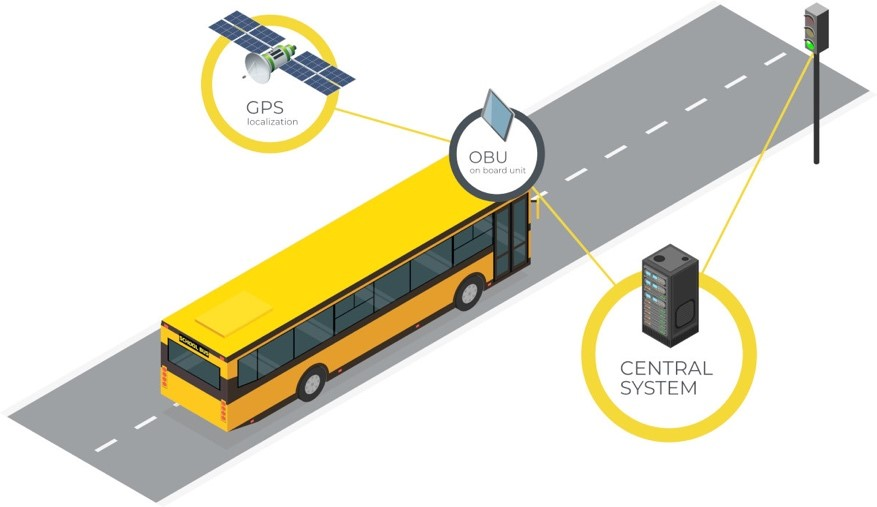
\includegraphics[width=0.7\linewidth]{image/pt_priority_system} \caption{Smart priority for public transport (SWARCO, 2021)}\label{fig:unnamed-chunk-10}
\end{figure}

\hypertarget{relevante-initiativen-in-uxf6sterreich-5}{%
\subsection*{Relevante Initiativen in Österreich}\label{relevante-initiativen-in-uxf6sterreich-5}}
\addcontentsline{toc}{subsection}{Relevante Initiativen in Österreich}

\begin{itemize}
\tightlist
\item
  \href{https://digitales.wien.gv.at/site/open-data/}{digitales.wien.gv.at}
\item
  \href{https://www.wienerlinien.at/eportal3/ep/channelView.do/pageTypeId/66528/channelId/-4400661}{wienerlinien.at}
\item
  \href{https://www.kapsch.net/ktc/Portfolio/IMS/Congestion/Managed-lanes}{kapsch.net-1}
\item
  \href{https://www.kapsch.net/ktc/Portfolio/IMS/Smart-Urban-Mobility/Urban-Mobility-Management}{kapsch.net-2}
\item
  \href{https://www.swarco.com/de/loesungen/oeffentlicher-nahverkehr/vorrang-fuer-den-oeffentlichen-nahverkehr}{swarco.com}
\item
  \href{https://www.mobility.siemens.com/global/de/portfolio/strasse/verkehrsmanagement/auf-der-strasse/smart-detection.html}{mobility.siemens.com}
\end{itemize}

\hypertarget{auswirkungen-in-bezug-auf-die-ziele-fuxfcr-nachhaltige-entwicklung-sdgs-5}{%
\subsection*{Auswirkungen in Bezug auf die Ziele für nachhaltige Entwicklung (SDGs)}\label{auswirkungen-in-bezug-auf-die-ziele-fuxfcr-nachhaltige-entwicklung-sdgs-5}}
\addcontentsline{toc}{subsection}{Auswirkungen in Bezug auf die Ziele für nachhaltige Entwicklung (SDGs)}

\begin{longtable}[]{@{}ccccc@{}}
\toprule
\begin{minipage}[b]{0.17\columnwidth}\centering
Ebene der Auswirkungen\strut
\end{minipage} & \begin{minipage}[b]{0.16\columnwidth}\centering
Indikator\strut
\end{minipage} & \begin{minipage}[b]{0.17\columnwidth}\centering
Richtung der Auswirkungen\strut
\end{minipage} & \begin{minipage}[b]{0.17\columnwidth}\centering
Beschreibung des Ziels \& SDG\strut
\end{minipage} & \begin{minipage}[b]{0.17\columnwidth}\centering
Quelle\strut
\end{minipage}\tabularnewline
\midrule
\endhead
\begin{minipage}[t]{0.17\columnwidth}\centering
Individuell\strut
\end{minipage} & \begin{minipage}[t]{0.16\columnwidth}\centering
Mehr Gleichheit fuer Menschen, die nicht Auto fahren\strut
\end{minipage} & \begin{minipage}[t]{0.17\columnwidth}\centering
\textbf{+}\strut
\end{minipage} & \begin{minipage}[t]{0.17\columnwidth}\centering
Gleichheit (\emph{5,10})\strut
\end{minipage} & \begin{minipage}[t]{0.17\columnwidth}\centering
Litman, 2017; Cervero, 2013\strut
\end{minipage}\tabularnewline
\begin{minipage}[t]{0.17\columnwidth}\centering
Individuell\strut
\end{minipage} & \begin{minipage}[t]{0.16\columnwidth}\centering
Weniger Reisezeit fuer Nutzer:innen oeffentlicher Verkehrsmittel, mehr Reisezeit fuer Pkw-Nutzer\strut
\end{minipage} & \begin{minipage}[t]{0.17\columnwidth}\centering
\textbf{\textasciitilde{}}\strut
\end{minipage} & \begin{minipage}[t]{0.17\columnwidth}\centering
Nachhaltige wirtschaftliche Entwicklung (\emph{8,11})\strut
\end{minipage} & \begin{minipage}[t]{0.17\columnwidth}\centering
Seredynski et al., 2015\strut
\end{minipage}\tabularnewline
\begin{minipage}[t]{0.17\columnwidth}\centering
Systemisch\strut
\end{minipage} & \begin{minipage}[t]{0.16\columnwidth}\centering
Der oeffentliche Verkehr wird im Vergleich zu anderen Verkehrstraegern wettbewerbsfaehiger\strut
\end{minipage} & \begin{minipage}[t]{0.17\columnwidth}\centering
\textbf{+}\strut
\end{minipage} & \begin{minipage}[t]{0.17\columnwidth}\centering
Gleichheit (\emph{5,10})\strut
\end{minipage} & \begin{minipage}[t]{0.17\columnwidth}\centering
Schwendinger, 2019\strut
\end{minipage}\tabularnewline
\begin{minipage}[t]{0.17\columnwidth}\centering
Systemisch\strut
\end{minipage} & \begin{minipage}[t]{0.16\columnwidth}\centering
Weniger Kraftstoffverbrauch\strut
\end{minipage} & \begin{minipage}[t]{0.17\columnwidth}\centering
\textbf{+}\strut
\end{minipage} & \begin{minipage}[t]{0.17\columnwidth}\centering
Oekologische Nachhaltigkeit (\emph{7,12,13,15})\strut
\end{minipage} & \begin{minipage}[t]{0.17\columnwidth}\centering
Gassel et al., 2012; Seredynski et al., 2015\strut
\end{minipage}\tabularnewline
\begin{minipage}[t]{0.17\columnwidth}\centering
Systemisch\strut
\end{minipage} & \begin{minipage}[t]{0.16\columnwidth}\centering
Der Transit ist oft der kostenguenstigste Verkehrstraeger\strut
\end{minipage} & \begin{minipage}[t]{0.17\columnwidth}\centering
\textbf{+}\strut
\end{minipage} & \begin{minipage}[t]{0.17\columnwidth}\centering
Nachhaltige wirtschaftliche Entwicklung (\emph{8,11})\strut
\end{minipage} & \begin{minipage}[t]{0.17\columnwidth}\centering
Litman, 2015\strut
\end{minipage}\tabularnewline
\begin{minipage}[t]{0.17\columnwidth}\centering
Systemisch\strut
\end{minipage} & \begin{minipage}[t]{0.16\columnwidth}\centering
Mehr Infrastruktur fuer den oeffentlichen Verkehr\strut
\end{minipage} & \begin{minipage}[t]{0.17\columnwidth}\centering
\textbf{+}\strut
\end{minipage} & \begin{minipage}[t]{0.17\columnwidth}\centering
Innovation und Infrastruktur (\emph{9})\strut
\end{minipage} & \begin{minipage}[t]{0.17\columnwidth}\centering
Cuthill et al., 2019\strut
\end{minipage}\tabularnewline
\bottomrule
\end{longtable}

\hypertarget{technologie--und-gesellschaftlicher-bereitschaftsgrad-3}{%
\subsection*{Technologie- und gesellschaftlicher Bereitschaftsgrad}\label{technologie--und-gesellschaftlicher-bereitschaftsgrad-3}}
\addcontentsline{toc}{subsection}{Technologie- und gesellschaftlicher Bereitschaftsgrad}

\begin{longtable}[]{@{}cc@{}}
\toprule
Stand der Technologiebereitschaft & Gesellschaftlicher Bereitschaftsgrad\tabularnewline
\midrule
\endhead
4-8 & 5-8\tabularnewline
\bottomrule
\end{longtable}

\hypertarget{offene-fragen-5}{%
\subsection*{Offene Fragen}\label{offene-fragen-5}}
\addcontentsline{toc}{subsection}{Offene Fragen}

\begin{enumerate}
\def\labelenumi{\arabic{enumi}.}
\tightlist
\item
  Wer ist für die Einführung von PTP-Systemen verantwortlich?
\item
  Wie werden Vehicle-to-Vehicle (V2V), Vehicle-to-Infrastructure (V2I) und in Zukunft Vehicle-to-Pedestrian (V2P) PTP-Systeme verändern?
\item
  Wie könnten auch Einsatzfahrzeuge priorisiert werden?
\item
  Wie geht man mit gemischten Flotten um - halb neu, halb alt?
\item
  Was sind die Vorteile im Vergleich zu den Kosten?
\item
  Welche Standards sollten verwendet werden?
\end{enumerate}

\hypertarget{referenzen-5}{%
\subsection*{Referenzen}\label{referenzen-5}}
\addcontentsline{toc}{subsection}{Referenzen}

\begin{itemize}
\tightlist
\item
  Cervero, R. (2013). Bus rapid transit (BRT): An efficient and competitive mode of public transport (No.~2013-01). Working Paper.
\item
  Cuthill, N., Cao, M., Liu, Y., Gao, X., \& Zhang, Y. (2019). The association between urban public transport infrastructure and social equity and spatial accessibility within the urban environment: An investigation of Tramlink in London. Sustainability, 11(5), 1229.
\item
  Figenbaum, E., Fearnley, N., Pfaffenbichler, P., Hjorthol, R., Kolbenstvedt, M., Jellinek, R., \ldots{} \& Iversen, L. M. (2015). Increasing the competitiveness of e-vehicles in Europe. European transport research review, 7(3), 1-14.
\item
  Gassel, C., Matschek, T., \& Krimmling, J. (2012). Cooperative traffic signals for energy efficient driving in tramway systems. Aspekte der Verkehrstelematik--ausgewählte Veröffentlichungen 2012, 1.
\item
  Haitao, H., Yang, K., Liang, H., Menendez, M., \& Guler, S. I. (2019). Providing public transport priority in the perimeter of urban networks: A bimodal strategy. Transportation Research Part C: Emerging Technologies, 107, 171-192.
\item
  Litman, T. (2015). Evaluating public transit benefits and costs. Victoria, BC, Canada: Victoria Transport Policy Institute.
\item
  Litman, T. (2017). Evaluating Transportation Diversity. Victoria Transport Policy Institute.
\item
  Schwendinger, M. (2019). Vorrang für Busse und Straßenbahnen in Städten. \url{https://vcoe.at/files/vcoe/uploads/Projekte/Factsheets} 2019 Neu/VCÖ-Factsheet ÖV-Bevorrangen.pdf
\item
  Seredynski, M., Khadraoui, D., \& Viti, F. (2015, October). Signal phase and timing (SPaT) for cooperative public transport priority measures. In Proc. 22nd ITS World Congress.
\item
  Seredynski, M., Ruiz, P., Szczypiorski, K., \& Khadraoui, D. (2014, May). Improving bus ride comfort using GLOSA-based dynamic speed optimisation. In 2014 IEEE International Parallel \& Distributed Processing Symposium Workshops (pp.~457-463). IEEE.
\item
  Seredynski, M., \& Viti, F. (2017, October). Novel C-ITS support for electric buses with opportunity charging. In 2017 IEEE 20th International Conference on Intelligent Transportation Systems (ITSC) (pp.~1-6). IEEE.
\item
  Stahlmann, R., Möller, M., Brauer, A., German, R., \& Eckhoff, D. (2018). Exploring GLOSA systems in the field: Technical evaluation and results. Computer Communications, 120, 112-124.
\item
  SWARCO. (2021). Vorrang für den ÖPNV: Öffentliche Verkehrsmittel attraktiver machen. Available at: \url{https://www.swarco.com/de/loesungen/oeffentlicher-nahverkehr/vorrang-fuer-den-oeffentlichen-nahverkehr} {[}Accessed: 26 January 2021{]}
\item
  WIENER STADTWERKE GmbH. (2018). Wiener Linien: Autos auf Busspuren halten Ã--ffis auf. Available at: \url{https://www.wienerstadtwerke.at/eportal3/ep/contentView.do?pageTypeId=71954\&channelId=-51313\&programId=72863\&contentId=4202309\&contentTypeId=1001} {[}Accessed: 30 September 2021{]}
\end{itemize}

\hypertarget{transformation_public_space}{%
\section{Transformation des öffentlichen Raums und digitale Lösungen}\label{transformation_public_space}}

\hypertarget{definition-6}{%
\subsection*{Definition}\label{definition-6}}
\addcontentsline{toc}{subsection}{Definition}

Die Digitalisierung des öffentlichen (und städtischen) Raums hat sich entwickelt und zu Konzepten wie Smart City, Wise City, U-City, intelligente Stadt usw. geführt. Die eigentliche Beschleunigung begann jedoch in den 2010er Jahren als Ergebnis von Initiativen der Industrie, die sich auf die Sammlung, Verwaltung, Verarbeitung und Echtzeitanalyse von Big Data durch die weit verbreiteten Sensoren in städtischen Räumen, die als Internet of Things (IoT)-Geräte bekannt sind, konzentrieren. In den letzten Jahren, insbesondere seit dem Ausbruch der COVID-19-Pandemie, hat die Digitalisierung der Städte ein neues Niveau erreicht. So werden beispielsweise in China digitale Systeme zur Massenüberwachung auf der Grundlage der Gesichtserkennung eingesetzt, und in anderen Teilen der Welt wurden Rechtsgrundlagen (wie die Allgemeine Datenschutzverordnung (DSGVO)) entwickelt, um die Erfassung biometrischer Daten im öffentlichen Raum zu ermöglichen (Languillon-Aussel, 2021). Über die Überwachung hinaus wird die Digitalisierung des öffentlichen Raums in vielen verschiedenen Bereichen eingesetzt, z. B. bei Zahlungen und Preisgestaltung, partizipativen Instrumenten oder der Strafverfolgung. So hat Singapur 2020 ein satellitengestütztes städtisches Mautsystem eingeführt, das die Verfolgung jedes Fahrzeugs zu jeder Tageszeit ermöglicht, um eine dynamische Preisgestaltung für die Straßennutzung und den Zonenzugang umzusetzen (Languillon-Aussel, 2021).
Zu den aktuellen Ansätzen für die Digitalisierung des öffentlichen Raums gehören mobile Apps, hochauflösende Kameras, interaktive Stände und Kioske, die Dienstleistungen und Informationen anbieten, aber auch IoT-Geräte wie Sensoren und Beacons, die automatisch Daten sammeln. Diese Geräte haben das Potenzial, die Qualität und den Umfang der Dienstleistungen im öffentlichen Raum zu verbessern, die Bereitstellungs- und Lieferkosten zu senken und die Sicherheit zu erhöhen. Dennoch sind sie nicht ohne Herausforderungen. Potenzielle Probleme ergeben sich aus Datenschutz- und Sicherheitsbedenken, insbesondere wenn der private Sektor eine Schlüsselrolle spielt (Warbis, 2018), aus potenziellen technischen Schwierigkeiten wie unzuverlässigen Internetverbindungen oder instabiler Stromversorgung (Haldrup, 2018) sowie aus geringem Vertrauen unter den Mitgliedern der Gesellschaft und der so genannten digitalen Ausgrenzung bestimmter sozialer Gruppen (Durand \& Zijlstra, 2020).

\hypertarget{wichtige-interessensgruppen-6}{%
\subsection*{Wichtige Interessensgruppen}\label{wichtige-interessensgruppen-6}}
\addcontentsline{toc}{subsection}{Wichtige Interessensgruppen}

\begin{itemize}
\tightlist
\item
  \textbf{Betroffene}: Bürger:innen
\item
  \textbf{Verantwortliche}: Lokale und nationale Regierungen, private Technologieunternehmen, Bürger:innen
\end{itemize}

\hypertarget{aktueller-stand-der-wissenschaft-und-forschung-6}{%
\subsection*{Aktueller Stand der Wissenschaft und Forschung}\label{aktueller-stand-der-wissenschaft-und-forschung-6}}
\addcontentsline{toc}{subsection}{Aktueller Stand der Wissenschaft und Forschung}

Die Forschung zeigt, dass infolge der zunehmenden Digitalisierung des öffentlichen Raums und insbesondere der zunehmenden Digitalisierung des Verkehrs einige Gruppen digital ausgeschlossen werden können. Die Faktoren, die mit der Anfälligkeit in Bezug auf den Zugang zu digital gestützten Dienstleistungen und Verkehrsmitteln verbunden sind, sind:

\begin{itemize}
\tightlist
\item
  \textbf{Alter}: Ältere Menschen und Minderjährige sind aufgrund ihres geringeren Engagements für Technologie besonders benachteiligt. Im Falle der älteren Bevölkerung bedeuten die Verringerung der kognitiven Fähigkeiten und ein Rückgang der psychologischen Mechanismen, dass der Umgang mit neuen Technologien im Allgemeinen schwierig sein kann (Harvey et al., 2019; Pangbourne et al., 2010; Durand \& Zijlstra, 2020). Andererseits haben Kinder häufig keinen Zugang zu digitalen Zahlungsmitteln oder können nicht alle verfügbaren Verkehrsmittel allein nutzen (Durand \& Zijlstra, 2020).
\item
  \textbf{Einkommen und Bildungsniveau}: Menschen mit geringerem Einkommen und Bildungsniveau sind anfälliger für digitale Ausgrenzung, wobei beispielsweise ein niederländischer Bericht zeigt, dass der Übergang vom Offline- zum Online-Kauf eines Jahresabonnements für öffentliche Verkehrsmittel für Menschen mit geringerem Einkommen problematisch ist (Durand \& Zijlstra, 2020).
\item
  \textbf{Ethnische Zugehörigkeit}: Personen, die Minderheiten angehören, sind tendenziell stärker benachteiligt, was jedoch häufig mit anderen Faktoren wie kulturellen Präferenzen oder wirtschaftlicher Benachteiligung zusammenhängt (Durand \& Zijlstra, 2020).
\end{itemize}

\hypertarget{aktueller-stand-der-praktischen-umsetzung-6}{%
\subsection*{Aktueller Stand der praktischen Umsetzung}\label{aktueller-stand-der-praktischen-umsetzung-6}}
\addcontentsline{toc}{subsection}{Aktueller Stand der praktischen Umsetzung}

Zu Beginn stützte sich die Digitalisierung von Städten und öffentlichen Räumen stark auf das verborgene, unterirdische Netz von Kabeln, Sensoren, Steckern und Masten, die im Alltag des Durchschnittsbürgers keine große Rolle spielten. Heutzutage bezieht die Digitalisierung des öffentlichen Raums das Konzept der Smart City in viel größerem Umfang in das tägliche Leben ein. Es gibt viele Möglichkeiten, wie die Digitalisierung im öffentlichen Raum umgesetzt werden kann.

Eine davon ist die verbesserte \textbf{Konnektivität } in Form von Wi-Fi-Hotspots und -Zonen. In New York hat \href{https://www.link.nyc/}{LinkNYC} beispielsweise Konnektivitätskorridore in fünf Bezirken mit mehr als 1700 Verbindungen eingerichtet und damit rund 5 Millionen Nutzer:innen ermöglicht sich kostenlos mit dem schnellsten und stabilsten öffentlichen Glasfasernetz des Landes zu verbinden. Durch diesen Dienst hat LinkNYC den Menschen den Zugang zu Wohltätigkeitsorganisationen, die Nutzung von Behördendiensten und sogar die Bewerbung um einen Arbeitsplatz ermöglicht (Warbis, 2018). Darüber hinaus nutzt \href{https://calvium.com/}{Calvium} die verbesserte Konnektivität, um durch digital-physische Reisen in die Geschichte und das Erbe einen Sinn für den Ort zu schaffen, wie etwa in der \href{https://calvium.com/projects/battersea-power-station-redevelopment/}{Battersea Power Station} in London (Warbis, 2018).

Darüber hinaus bringt die Digitalisierung eine \textbf{Transformation der öffentlichen Dienstleistungen} mit sich, bei der nicht personenbezogene Daten, die im öffentlichen Raum erhoben werden, genutzt werden, um die Nutzer:innen des öffentlichen Raums und ihre Bedürfnisse besser zu verstehen, um die Räume, die Infrastruktur und die Bereitstellung öffentlicher Dienstleistungen in den Städten zu verbessern. Wenn man sich beispielsweise die Art der Geräte ansieht, die mit WiFi-Spots verbunden sind, oder wenn man sich an einem digitalen Platzgestaltungsprogramm beteiligt, kann man sozioökonomische Profile erkennen und die Stadtverwaltungen dabei unterstützen, die richtigen Dienstleistungen für die richtigen Menschen bereitzustellen.

Zwei solcher Beispiele sind (1) der (\emph{1}) \href{https://lbbd.emu-analytics.net/main/(view/950db2c7-1a3b-448d-9b21-444a0ec7b5e0//rightBar:appinfo)?basemapDetail=1\&zoom=5.0\&lng=-0.36613\&lat=54.04187}{Borough Data Explorer}, der Daten für die Indikatoren sammelt, die entweder zu den sogenannten Borough Manifesto-Zielen der Stadt beitragen oder im sozialen Fortschrittsindex der Stadt enthalten sind (Lbbd.emu-analytics.net, 2021). (2) Die australische Stadt Joondalup ist eine Partnerschaft mit \href{https://www.lakesidejoondalup.com.au/store-directory/telstra-shop/}{Telstra} eingegangen, um IoT-Technologien zu testen, mit denen Umweltfaktoren wie Temperatur, Luftfeuchtigkeit, Verschmutzung, Licht- und Lärmpegel in Echtzeit besser überwacht werden können (Barns, 2017).

Als Nächstes ist eine \textbf{öffentlich-private Partnerschaft} von entscheidender Bedeutung für einen starken und zuverlässigen digitalen öffentlichen Bereich, in dem Technologieunternehmen die Politik und Strategie der lokalen Regierung verstehen müssen, um Bereiche zu ermitteln, die durch den digitalen Einsatz unterstützt werden können. Auf der anderen Seite ist es für die Kommunalverwaltung wichtig, die Merkmale der einzusetzenden Technologie zu verstehen. Diese enge Zusammenarbeit ermöglicht es dem öffentlichen Sektor, die Digitalisierung von Orten so zu lenken, dass sie dem öffentlichen Wohl dient und der öffentliche Charakter von Raum und Ort erhalten bleibt, unabhängig davon, wer die eingesetzten Technologien besitzt, beaufsichtigt oder verwaltet (Warbis, 2018). Beispiele für solche Initiativen sind \href{https://wegfinder.at/presse/2021/mit-wegfinder-ist-mobility-as-a-service-in-oesterreich-angekommen(1)/}{Ã--BB360 wegfinder}, \href{https://austriatech.at/en/insight-into-the-work-of-the-urban-mobility-laboratories/}{Living Labs} und \href{https://www.aspern-seestadt.at/en}{Seestadt Wien}.

Innerhalb des Verkehrsnetzes bringt die Digitalisierung Vorteile in Form von verbesserter Individualisierung, Effizienz und Komfort. Beispiele dafür sind Echtzeitinformationen über verfügbare Parkplätze wie \href{https://www.eparkomat.com/}{eParkomat} in der Tschechischen Republik, digitales Ticketing und Fahrplanauskunft wie, \href{https://www.dv-ticketing.com/}{DV Ticketing} oder \href{https://www.thetrainline.com/}{Trainline} in Großbritannien, elektronische Systeme für Car- und Bike-Sharing-Flotten wie \href{https://www.share-now.com/at/en/}{Share-now} oder \href{https://www.nextbike.at/de/niederoesterreich/}{Nextbike} usw. Weitere Informationen über Bike- und Carsharing finden Sie in den Abschnitten über \protect\hyperlink{bike_sharing}{Fahrrad- und E-Bike-Verleih} und \protect\hyperlink{car_sharing}{Car Sharing} in dieser Arbeit.

Schließlich wird behauptet, dass der öffentliche Raum eine politische Funktion hat. In Europa unterstützen und bestimmen sie den Ausdruck des Lebens in der Stadt und spielen eine Rolle bei der partizipativen Planung (Languillon-Aussel, 2021; Parkinson, 2012). So beabsichtigten beispielsweise die österreichischen Eisenbahnen (ÖBB) 2013 den Bau eines\href{https://www.partizipation.at/gueterzentrum_sued.html}{neuen Güterverkehrszentrums} in Wien, das den Güterverkehr von der Straße auf die Schiene verlagern sollte. Das neue Güterverkehrszentrum sollte dasjenige am Nordwestbahnhof ersetzen. Von Anfang an sollte die Öffentlichkeit aktiv in das Projekt einbezogen werden, und die Betroffenen wurden auch stark in die Planung integriert. So gab es vor Projektbeginn eine Informationsveranstaltung der ÖBB, die von großen Protesten (der Bevölkerung) gegen das Projekt begleitet war. Die ÖBB haben wohl gerade deshalb versucht, die Entscheidungsträger:innen so intensiv in den gesamten Planungsprozess einzubinden und haben das Projekt in der Folge erfolgreich abgeschlossen.

Daher kann die Digitalisierung des städtischen Raums die Innovation bei den partizipatorischen Instrumenten beeinflussen, die es den Bürger:innen ermöglichen, ihre Meinung zu äußern und Feedback zu geben, um aktiv zum Infrastrukturplanungsprozess und zur Entscheidungsfindung beizutragen. Dieser Trend führte zur sogenannten digitalen partizipativen Planung (DPP) (Bouzguenda et al., 2020). Einige Beispiele für solche Initiativen sind die App \href{https://mapyour.city/}{Map your city} die Ideenfindungsplattform \href{https://www.involve.org.uk/resources/case-studies/decide-madrid}{Decide Madrid}, \href{https://oscity.nl/}{Open Source City} in den Niederlanden, die britischen Feedback-Plattformen \href{https://www.involve.org.uk/resources/knowledge-base/what/public-participation}{Involve} und \href{http://www.changify.org/}{Changify} oder die Visualisierungsplattform für Argumente namens \href{https://www.nesta.org.uk/feature/six-pioneers-digital-democracy/vtaiwan/}{vTaiwan}.

\hypertarget{relevante-initiativen-in-uxf6sterreich-6}{%
\subsection*{Relevante Initiativen in Österreich}\label{relevante-initiativen-in-uxf6sterreich-6}}
\addcontentsline{toc}{subsection}{Relevante Initiativen in Österreich}

\begin{itemize}
\tightlist
\item
  \href{https://wegfinder.at/presse/2021/mit-wegfinder-ist-mobility-as-a-service-in-oesterreich-angekommen(1)/}{Ã--BB360 wegfinder}
\item
  \href{https://austriatech.at/en/insight-into-the-work-of-the-urban-mobility-laboratories/}{Living Labs}
\item
  \href{https://www.aspern-seestadt.at/en}{Seestadt Wien}
\item
  \href{https://ec.europa.eu/regional_policy/en/projects/Austria/support-for-digital-transformation-in-lower-austria}{House of digitalisation}
\end{itemize}

\hypertarget{auswirkungen-in-bezug-auf-die-ziele-fuxfcr-nachhaltige-entwicklung-sdgs-6}{%
\subsection*{Auswirkungen in Bezug auf die Ziele für nachhaltige Entwicklung (SDGs)}\label{auswirkungen-in-bezug-auf-die-ziele-fuxfcr-nachhaltige-entwicklung-sdgs-6}}
\addcontentsline{toc}{subsection}{Auswirkungen in Bezug auf die Ziele für nachhaltige Entwicklung (SDGs)}

\begin{longtable}[]{@{}ccccc@{}}
\toprule
\begin{minipage}[b]{0.17\columnwidth}\centering
Ebene der Auswirkungen\strut
\end{minipage} & \begin{minipage}[b]{0.16\columnwidth}\centering
Indikator\strut
\end{minipage} & \begin{minipage}[b]{0.17\columnwidth}\centering
Richtung der Auswirkungen\strut
\end{minipage} & \begin{minipage}[b]{0.17\columnwidth}\centering
Beschreibung des Ziels \& SDG\strut
\end{minipage} & \begin{minipage}[b]{0.17\columnwidth}\centering
Quelle\strut
\end{minipage}\tabularnewline
\midrule
\endhead
\begin{minipage}[t]{0.17\columnwidth}\centering
Individuell\strut
\end{minipage} & \begin{minipage}[t]{0.16\columnwidth}\centering
Verschlechterter Zugang zu digital gestuetzten Verkehrsdiensten fuer bestimmte Gruppen\strut
\end{minipage} & \begin{minipage}[t]{0.17\columnwidth}\centering
\textbf{-}\strut
\end{minipage} & \begin{minipage}[t]{0.17\columnwidth}\centering
Gleichheit (\emph{5,10})\strut
\end{minipage} & \begin{minipage}[t]{0.17\columnwidth}\centering
Durand \& Zijlstra, 2020\strut
\end{minipage}\tabularnewline
\begin{minipage}[t]{0.17\columnwidth}\centering
Systemisch\strut
\end{minipage} & \begin{minipage}[t]{0.16\columnwidth}\centering
Geringeres Risiko der verkehrsbedingten sozialen Ausgrenzung\strut
\end{minipage} & \begin{minipage}[t]{0.17\columnwidth}\centering
\textbf{+}\strut
\end{minipage} & \begin{minipage}[t]{0.17\columnwidth}\centering
Gleichheit (\emph{5,10})\strut
\end{minipage} & \begin{minipage}[t]{0.17\columnwidth}\centering
Harvey et al., 2019; Pangbourne et al., 2010\strut
\end{minipage}\tabularnewline
\begin{minipage}[t]{0.17\columnwidth}\centering
Systemisch\strut
\end{minipage} & \begin{minipage}[t]{0.16\columnwidth}\centering
Besser informierte Planung und Entscheidungsfindung auf der Grundlage von Echtzeitdaten aus dem IoT\strut
\end{minipage} & \begin{minipage}[t]{0.17\columnwidth}\centering
\textbf{+}\strut
\end{minipage} & \begin{minipage}[t]{0.17\columnwidth}\centering
Innovation und Infrastruktur (\emph{9})\strut
\end{minipage} & \begin{minipage}[t]{0.17\columnwidth}\centering
Barns, 2017, Bouzguenda et al., 2020\strut
\end{minipage}\tabularnewline
\begin{minipage}[t]{0.17\columnwidth}\centering
Systemisch\strut
\end{minipage} & \begin{minipage}[t]{0.16\columnwidth}\centering
Verstaerkte Zusammenarbeit zwischen oeffentlichem und privatem Sektor\strut
\end{minipage} & \begin{minipage}[t]{0.17\columnwidth}\centering
\textbf{+}\strut
\end{minipage} & \begin{minipage}[t]{0.17\columnwidth}\centering
Partnerschaften und Kooperationen (\emph{17})\strut
\end{minipage} & \begin{minipage}[t]{0.17\columnwidth}\centering
Warbis, 2018;\strut
\end{minipage}\tabularnewline
\bottomrule
\end{longtable}

\hypertarget{technologie--und-gesellschaftlicher-bereitschaftsgrad-4}{%
\subsection*{Technologie- und gesellschaftlicher Bereitschaftsgrad}\label{technologie--und-gesellschaftlicher-bereitschaftsgrad-4}}
\addcontentsline{toc}{subsection}{Technologie- und gesellschaftlicher Bereitschaftsgrad}

\begin{longtable}[]{@{}cc@{}}
\toprule
Stand der Technologiebereitschaft & Gesellschaftlicher Bereitschaftsgrad\tabularnewline
\midrule
\endhead
5-9 & 5-8\tabularnewline
\bottomrule
\end{longtable}

\hypertarget{offene-fragen-6}{%
\subsection*{Offene Fragen}\label{offene-fragen-6}}
\addcontentsline{toc}{subsection}{Offene Fragen}

\begin{enumerate}
\def\labelenumi{\arabic{enumi}.}
\tightlist
\item
  Inwieweit wirkt sich der immer wichtigere Einsatz digitaler Geräte im öffentlichen Raum auf dessen politische Dimensionen aus?
\item
  Verändern die digitalen Technologien die Praktiken der Bürger:innen im öffentlichen Raum und/oder ermöglichen sie das Entstehen neuer Praktiken?
\item
  Indem sie neue Formen der Meinungsäußerung sowie der politischen und demokratischen Teilhabe im Internet ermöglichen, wird der virtuelle Raum tendenziell zu einem neuen Forum. Übernimmt die digitale Technologie die politischen Funktionen des öffentlichen Raums, der dadurch überflüssig geworden ist?
\item
  Welche Auswirkungen haben die kurzen Lebenszyklen der Technologien und der Wechsel der Technologiegenerationen auf die Entwicklung des öffentlichen Raums?
\item
  Verändert die Digitalisierung das Design, die Formen, die Dimensionen und die Räumlichkeit des öffentlichen Raums?
\item
  Auf welche Weise verändert das Aufkommen neuer Werkzeuge und Fähigkeiten die Art und Weise, wie öffentliche Räume geplant und entwickelt werden?
\item
  Welche Rolle spielen digitale Technologien bei der Darstellung, Vorstellung und Wahrnehmung von öffentlichen Räumen?
\item
  Für welche(n) Typ(en) von Empfängern (wie Bürger:innen, Verbraucher:innen, Nutzer:innen und Bewohner:innen) werden digitale Technologien im öffentlichen Raum eingesetzt?
\item
  Welche Auswirkungen haben sie auf die Menschen, die sich im öffentlichen Raum aufhalten?
\item
  Fördern die digitalen Technologien den sozialen Austausch oder vervielfältigen sie im Gegenteil die Segregation der digitalen Blasen?
\item
  Welche Rolle hat die Digitalisierung bei der Anpassung des öffentlichen Raums an die Gesundheitskrise von COVID-19 gespielt? (Languillon-Aussel, 2021)
\end{enumerate}

\hypertarget{weitere-links-4}{%
\subsection*{Weitere links}\label{weitere-links-4}}
\addcontentsline{toc}{subsection}{Weitere links}

\begin{itemize}
\tightlist
\item
  \href{https://agile-city.com/agile-city-research/digital-tools-for-participatory-led-design/}{Agile city}
\item
  \href{https://theconversation.com/surprise-digital-space-isnt-replacing-public-space-and-might-even-help-make-it-better-87173}{An article on city of bits}
\item
  \href{https://archer-soft.com/blog/how-build-real-time-parking-availability-system}{Parking management systems}
\item
  \href{https://jsis.washington.edu/news/internet-of-things-and-privacy-in-public/}{Internet of Things and Privacy in Public}
\end{itemize}

\hypertarget{referenzen-6}{%
\subsection*{Referenzen}\label{referenzen-6}}
\addcontentsline{toc}{subsection}{Referenzen}

\begin{itemize}
\tightlist
\item
  Barns, S. (2017) Surprise! Digital space isn't replacing public space, and might even help make it better. Available at: \url{https://theconversation.com/surprise-digital-space-isnt-replacing-public-space-and-might-even-help-make-it-better-87173} {[}Accessed: 12 April 2021{]}.
\item
  Bouzguenda, I., Alalouch, C., \& Fava, N. (2020). Examining digital participatory planning: maturity assessment in a small Dutch city. Journal of Cleaner Production, 264, 121706.
\item
  Durand, A. \& Zijlstra, T. (2020). The impact of digitalisation on the access to transport services: a literature review. 10.13140/RG.2.2.22686.97600.
\item
  Haldrup, S.,V. (2018). Digitising public service delivery: opportunities and limitations. Available at: \url{https://www.opml.co.uk/blog/digitising-public-service-delivery-opportunities-and-limitations} {[}Accessed: 12 April 2021{]}.
\item
  Harvey, J., Guo, W., \& Edwards, S. (2019). Increasing mobility for older travellers through engagement with technology. Transportation Research Part F: Traffic Psychology and Behaviour, 60, 172-184. \url{doi:10.1016/j.trf.2018.10.019}
\item
  Languillon-Aussel, R. (2021). Digitalisation of public spaces: the great urban change? Available at: \url{https://journals.openedition.org/articulo/4518} . {[}Accessed: 9 April 2021{]}
\item
  Lbbd.emu-analytics.net. (2021). Borough Data Explorer. Available at: \url{https://lbbd.emu-analytics.net/main/(view/950db2c7-1a3b-448d-9b21-444a0ec7b5e0//rightBar:appinfo)?basemapDetail=1\&zoom=4.7\&lng=3.34490\&lat=54.11363} {[}Accessed: 12 April 2021{]}.
\item
  Pangbourne, K. (2018). Mobility and Ageing: A Review of Interactions Between Transport and Technology from the Perspective of Older People In A. Curl \& C. Musselwhite (Eds.), Geographies of Transport and Ageing (pp.~51-71). Cham: Springer International Publishing.
\item
  Parkinson J., 2012, Democracy and Public Space: The Physical Sites of Democratic Performance, Oxford: Oxford University Press, 262 p.
\item
  Warbis, M. (2018). Making the Spaces of Cities Smarter: Why cities (and their citizens) should embrace the digital public realm. \textless Available at: \url{https://medium.com/@warbismichelle/making-the-spaces-of-cities-smarter-why-cities-should-embrace-the-digital-public-realm-c12afc810aaa}\textgreater. {[}Accessed: 12 April 2021{]}
\end{itemize}

\hypertarget{highway}{%
\chapter{Verwaltung der Straßenverkehrsinfrastruktur}\label{highway}}

\hypertarget{uav}{%
\section{Unbemannte Luftfahrzeuge für die Instandhaltung der Infrastruktur}\label{uav}}

\hypertarget{synonyme-6}{%
\subsection*{Synonyme}\label{synonyme-6}}
\addcontentsline{toc}{subsection}{Synonyme}

\emph{Drohnen, ferngesteuerte Fahrzeuge, ferngesteuerte Flugzeuge, Unmanned Aerial Vehicles (UAV)}

\hypertarget{definition-7}{%
\subsection*{Definition}\label{definition-7}}
\addcontentsline{toc}{subsection}{Definition}

Unbemannte Luftfahrzeuge (Unmanned Aerial Vehicles - UAVs), gemeinhin als Drohnen bekannt, sind vielversprechende Technologien, die bei der Inspektion und Datenerfassung für die Instandhaltung und Verwaltung von Infrastrukturen eingesetzt werden können. Dazu gehören zum Beispiel die Erkennung von Verschleiß, die Überwachung des Fortschritts auf einer Autobahnbaustelle oder die Analyse des Verkehrs (Frederiksen et al., 2019). UAVs verfügen in der Regel über eine tragbare Kontrollstation für den menschlichen Bediener, und nach den geltenden Rechtsvorschriften ist ihr Einsatz in städtischen Gebieten auf Flüge innerhalb der Sichtlinie (visual line of sight - VLOS) beschränkt. UAVs verfügen in der Regel über verschiedene Sensoren und Aufzeichnungsgeräte, darunter Video-, Fern- und Nahinfrarot-, Radar- oder Laser-Entfernungsmesser sowie spezielle Kommunikationsgeräte (Shaghlil \& Khalafallah, 2018). Die meisten von ihnen können Echtzeitdaten zwischen dem UAV und der Kontrollstation übertragen. Darüber hinaus verfügen einige von ihnen über zusätzliche Onboard-Datenspeicherfunktionen für eine verbesserte Datenerfassung (Shaghlil \& Khalafallah, 2018). Der Einsatz von Drohnen für infrastrukturbezogene Aufgaben führt nicht nur zu Zeit-, Arbeits- und Kosteneinsparungen, sondern ermöglicht auch eine Verringerung der Risiken, wenn gefährliche Tätigkeiten, die normalerweise von Menschen ausgeführt werden, durch Drohnen ersetzt werden können. Schließlich werden auch die Umweltauswirkungen verringert, wenn Drohnen, die erheblich weniger CO\textsubscript{2} produzieren, anstelle der derzeit eingesetzten Hubschrauber eingesetzt werden. Dennoch kann der Einsatz von Drohnen als Instrument zur Inspektion von Infrastrukturen auch gewisse Herausforderungen in Bezug auf die derzeitige Technologie, den rechtlichen Rahmen, den Schutz der Privatsphäre und die gesellschaftliche Akzeptanz mit sich bringen.

\hypertarget{wichtige-interessensgruppen-7}{%
\subsection*{Wichtige Interessensgruppen}\label{wichtige-interessensgruppen-7}}
\addcontentsline{toc}{subsection}{Wichtige Interessensgruppen}

\begin{itemize}
\tightlist
\item
  \textbf{Betroffene}: Direkte Nutzer:innen der Straßen und Begünstigte, die von der Erbringung von Verkehrsdienstleistungen betroffen sind
\item
  \textbf{Verantwortliche}: Staatliche Stellen, die für die Planung, Durchführung und Finanzierung von Instandhaltungsmaßnahmen zuständig sind, Bürger:innen, Auftragnehmer:innen und Unterauftragnehmer:innen, Privatunternehmen und Hersteller
\end{itemize}

\hypertarget{aktueller-stand-der-wissenschaft-und-forschung-7}{%
\subsection*{Aktueller Stand der Wissenschaft und Forschung}\label{aktueller-stand-der-wissenschaft-und-forschung-7}}
\addcontentsline{toc}{subsection}{Aktueller Stand der Wissenschaft und Forschung}

Aktuelle Forschungsanstrengungen und auf Feldversuchen basierende Studien sprechen für den Einsatz von UAVs zur Brückeninspektion und -überwachung. In einer früheren Studie wurde ein Konzeptnachweis für den Einsatz von UAVs für Brücken- und Hochmastleuchten vorgelegt. Es wurden mehrere Experimente unter kontrollierten Bedingungen durchgeführt, um das Verhalten von UAVs in Abhängigkeit von den Windverhältnissen zu testen. Außerdem wurde die Bildqualität in verschiedenen Flugszenarien, bei schlechten Lichtverhältnissen, in verschiedenen Höhen und mit unterschiedlicher Nutzlast untersucht (Otero et al., 2015). Insgesamt sprechen die Ergebnisse für den Einsatz von Drohnen bei Infrastrukturinspektionen, nicht nur im Hinblick auf die Einsparung menschlicher Arbeitskraft, sondern auch auf die Erkennung von Schäden. Die Vorteile des Drohneneinsatzes wurden auch im Hinblick auf eine geringere Verkehrskontrolle und einen geringeren Einsatz von Inspektionsfahrzeugen unter Brücken nachgewiesen (Zink und Lovelace, 2015). Andererseits wurde festgestellt, dass der Mangel an spezifischen Fähigkeiten der Drohnenbediener den effizienten Einsatz von Drohnen für große Brücken behindert (Wu et al., 2018). Darüber hinaus bremsen auch einige technologische Barrieren die Popularität von Drohnen bei der Infrastrukturinspektion, wobei die durchschnittliche Flugzeit der Drohne angesichts ihrer Akkulaufzeit etwa 30 Minuten beträgt. Daher zielt die aktuelle Forschung darauf ab, die Energieeffizienz durch den Einsatz von Pfadplanung und Algorithmen zur Minimierung des Energieverbrauchs bei gleichzeitiger Maximierung der Abdeckung für die Verkehrsüberwachung zu erhöhen (Outay et al., 2020).

\hypertarget{aktueller-stand-der-praktischen-umsetzung-7}{%
\subsection*{Aktueller Stand der praktischen Umsetzung}\label{aktueller-stand-der-praktischen-umsetzung-7}}
\addcontentsline{toc}{subsection}{Aktueller Stand der praktischen Umsetzung}

Die derzeitige Nutzung von Drohnen wird von nationalen und internationalen Regierungen weltweit stark reguliert, wobei die größte Einschränkung darin besteht, dass die Drohnen in der VLOS-Position des Fluglotsen bleiben müssen. Darüber hinaus legen die Regulierungsbehörden verschiedene Spezifikationen in Bezug auf physische Aspekte der Drohnen wie Gewicht oder Sensoren, Schulungsanforderungen für Betreiber und Drohnen, Vorschriften für die Datenerfassung und den Betrieb selbst wie Flugdauer, Flughöhe usw. vor. (FAA, 2016; Outay at al., 2020). Alle diese Faktoren schränken die schnelle und breite Anwendung von Drohnen in verschiedenen Bereichen erheblich ein. Daher versuchen die Behörden, Vorschriften zu erlassen, um die Bedenken der Bürger:innen in Bezug auf Sicherheit, Privatsphäre und Lärm zu zerstreuen. Gegenwärtig werden Drohnen in der Öl- und Gasindustrie eingesetzt, um lokale Erhebungen in Offshore-Anlagen durchzuführen (Unternehmen, 2016). Im Verkehrssektor hat das dänische Unternehmen Dronops nach einer Sicherheitsüberprüfung von der dänischen Straßenverkehrsbehörde die Genehmigung erhalten, entlang einer Autobahn zu fliegen, um den Verkehr zu überwachen, wobei die Drohne Daten von mehreren Sensoren sowie Videoaufnahmen liefert. Derzeit kann die Drohne nur bei guten Wetterbedingungen fliegen und ist per Kabel mit ihrer Stromquelle am Boden verbunden, um eine kontinuierliche Überwachung in 120 m Höhe den ganzen Tag lang zu ermöglichen. Wichtig ist, dass die ausgegebenen Daten von der dänischen Straßenverkehrsbehörde und der Gemeindeverwaltung verwendet werden (Frederiksen et al., 2019).

\hypertarget{relevante-initiativen-in-uxf6sterreich-7}{%
\subsection*{Relevante Initiativen in Österreich}\label{relevante-initiativen-in-uxf6sterreich-7}}
\addcontentsline{toc}{subsection}{Relevante Initiativen in Österreich}

\begin{itemize}
\tightlist
\item
  \href{https://smartcity.wien.gv.at/site/en/smart-inspection/}{smartcity.wien}
\end{itemize}

\hypertarget{auswirkungen-in-bezug-auf-die-ziele-fuxfcr-nachhaltige-entwicklung-sdgs-7}{%
\subsection*{Auswirkungen in Bezug auf die Ziele für nachhaltige Entwicklung (SDGs)}\label{auswirkungen-in-bezug-auf-die-ziele-fuxfcr-nachhaltige-entwicklung-sdgs-7}}
\addcontentsline{toc}{subsection}{Auswirkungen in Bezug auf die Ziele für nachhaltige Entwicklung (SDGs)}

\begin{longtable}[]{@{}ccccc@{}}
\toprule
\begin{minipage}[b]{0.17\columnwidth}\centering
Ebene der Auswirkungen\strut
\end{minipage} & \begin{minipage}[b]{0.16\columnwidth}\centering
Indikator\strut
\end{minipage} & \begin{minipage}[b]{0.17\columnwidth}\centering
Richtung der Auswirkungen\strut
\end{minipage} & \begin{minipage}[b]{0.17\columnwidth}\centering
Beschreibung des Ziels \& SDG\strut
\end{minipage} & \begin{minipage}[b]{0.17\columnwidth}\centering
Quelle\strut
\end{minipage}\tabularnewline
\midrule
\endhead
\begin{minipage}[t]{0.17\columnwidth}\centering
Individuell\strut
\end{minipage} & \begin{minipage}[t]{0.16\columnwidth}\centering
Verringerung des Risikos fuer Arbeitnehmer\strut
\end{minipage} & \begin{minipage}[t]{0.17\columnwidth}\centering
\textbf{+}\strut
\end{minipage} & \begin{minipage}[t]{0.17\columnwidth}\centering
Gesundheit und Wohlbefinden (\emph{3})\strut
\end{minipage} & \begin{minipage}[t]{0.17\columnwidth}\centering
Outay et al., 2020\strut
\end{minipage}\tabularnewline
\begin{minipage}[t]{0.17\columnwidth}\centering
Systemisch\strut
\end{minipage} & \begin{minipage}[t]{0.16\columnwidth}\centering
Erhoehung der Verkehrssicherheit\strut
\end{minipage} & \begin{minipage}[t]{0.17\columnwidth}\centering
\textbf{+}\strut
\end{minipage} & \begin{minipage}[t]{0.17\columnwidth}\centering
Gesundheit und Wohlbefinden (\emph{3})\strut
\end{minipage} & \begin{minipage}[t]{0.17\columnwidth}\centering
Outay et al., 2020\strut
\end{minipage}\tabularnewline
\begin{minipage}[t]{0.17\columnwidth}\centering
Systemisch\strut
\end{minipage} & \begin{minipage}[t]{0.16\columnwidth}\centering
Verringerte Emissionsrate\strut
\end{minipage} & \begin{minipage}[t]{0.17\columnwidth}\centering
\textbf{+}\strut
\end{minipage} & \begin{minipage}[t]{0.17\columnwidth}\centering
Oekologische Nachhaltigkeit (\emph{7,12,13,15})\strut
\end{minipage} & \begin{minipage}[t]{0.17\columnwidth}\centering
Outay et al., 2020\strut
\end{minipage}\tabularnewline
\begin{minipage}[t]{0.17\columnwidth}\centering
Systemisch\strut
\end{minipage} & \begin{minipage}[t]{0.16\columnwidth}\centering
Schaffung von Arbeitsplaetzen\strut
\end{minipage} & \begin{minipage}[t]{0.17\columnwidth}\centering
\textbf{+}\strut
\end{minipage} & \begin{minipage}[t]{0.17\columnwidth}\centering
Nachhaltige wirtschaftliche Entwicklung (\emph{8,11})\strut
\end{minipage} & \begin{minipage}[t]{0.17\columnwidth}\centering
Jenkins \& Vasigh, 2013\strut
\end{minipage}\tabularnewline
\begin{minipage}[t]{0.17\columnwidth}\centering
Systemisch\strut
\end{minipage} & \begin{minipage}[t]{0.16\columnwidth}\centering
Schnellere Innovation der Strasseninfrastruktur\strut
\end{minipage} & \begin{minipage}[t]{0.17\columnwidth}\centering
\textbf{+}\strut
\end{minipage} & \begin{minipage}[t]{0.17\columnwidth}\centering
Innovation und Infrastruktur (\emph{9})\strut
\end{minipage} & \begin{minipage}[t]{0.17\columnwidth}\centering
Fan \& Saadeghvaziri, 2019\strut
\end{minipage}\tabularnewline
\bottomrule
\end{longtable}

\hypertarget{technologie--und-gesellschaftlicher-bereitschaftsgrad-5}{%
\subsection*{Technologie- und gesellschaftlicher Bereitschaftsgrad}\label{technologie--und-gesellschaftlicher-bereitschaftsgrad-5}}
\addcontentsline{toc}{subsection}{Technologie- und gesellschaftlicher Bereitschaftsgrad}

\begin{longtable}[]{@{}cc@{}}
\toprule
Stand der Technologiebereitschaft & Gesellschaftlicher Bereitschaftsgrad\tabularnewline
\midrule
\endhead
3-4 & 5-7\tabularnewline
\bottomrule
\end{longtable}

\hypertarget{offene-fragen-7}{%
\subsection*{Offene Fragen}\label{offene-fragen-7}}
\addcontentsline{toc}{subsection}{Offene Fragen}

\begin{enumerate}
\def\labelenumi{\arabic{enumi}.}
\tightlist
\item
  Welche Faktoren beeinflussen die gesellschaftliche Akzeptanz von Drohnen?
\item
  Welche Maßnahmen müssen von den politischen Entscheidungsträger:innenn ergriffen werden, um Cyberangriffe auf ein Minimum zu reduzieren?
\item
  Welche Aspekte müssen von den Regierungen vor der Integration weiterer Sensoren zur Aufzeichnung anderer relevanter Daten sowie der Integration von Videodaten mit anderen Geodaten berücksichtigt werden?
\end{enumerate}

\hypertarget{weitere-links-5}{%
\subsection*{Weitere links}\label{weitere-links-5}}
\addcontentsline{toc}{subsection}{Weitere links}

\begin{itemize}
\tightlist
\item
  \href{https://www.rolandberger.com/en/Insights/Publications/Drones-The-future-of-asset-inspection.html}{rolandberger}
\end{itemize}

\hypertarget{referenzen-7}{%
\subsection*{Referenzen}\label{referenzen-7}}
\addcontentsline{toc}{subsection}{Referenzen}

\begin{itemize}
\tightlist
\item
  FAA News, 2016, Summary of Small Unmanned Aircraft Rule (Part 107), Federal Aviation Authority, Washington DC, 20591, Accessed on May 2020, \url{https://www.faa.gov/uas/media/Part_107_Summary.pdf}.
\item
  Fan, J., \& Saadeghvaziri, M. A. (2019). Applications of Drones in Infrastructures: Challenges and Opportunities. International Journal of Mechanical and Mechatronics Engineering, 13(10), 649-655.
\item
  Frederiksen, M. H., Mouridsen, O. A. V., \& Knudsen, M. P. (2019). Drones for inspection of infrastructure: Barriers, opportunities and successful uses.
\item
  Jenkins, D., \& Vasigh, B. (2013). The economic impact of unmanned aircraft systems integration in the United States. Association for Unmanned Vehicle Systems International (AUVSI).
\item
  Otero, L.D., Gagliardo, N., Dalli, D., Huang, W.-H., Cosentino, P. (2015). Proof of concept for using unmanned aerial vehicles for high mast pole and bridge inspections (No.~BDV28-977-02). Florida. Dept. of Transportation. Research Center.
\item
  Outay, F., Mengash, H. A., \& Adnan, M. (2020). Applications of unmanned aerial vehicle (UAV) in road safety, traffic and highway infrastructure management: Recent advances and challenges. Transportation research. Part A, Policy and practice, 141, 116-129. \url{https://doi.org/10.1016/j.tra.2020.09.018}
\item
  Shaghlil, N., \& Khalafallah, A. (2018). Automating highway infrastructure maintenance using unmanned aerial vehicles. In Construction Research Congress (2-4).
\item
  Undertaking, S. J. (2016). European drones outlook study. Unlocking the Value for Europe.
\item
  Wu, W., Qurishee, M. A., Owino, J., Fomunung, I., Onyango, M., Atolagbe, B. (2018). Coupling deep learning and UAV for infrastructure condition assessment automation. In: 2018 IEEE International Smart Cities Conference (ISC2). IEEE, pp.~1-7.
\item
  Zink, J. and Lovelace, B., 2015. Unmanned aerial vehicle bridge inspection demonstration project. Research Project. Final Report, 40. Accessed in Nov 2020
\end{itemize}

\hypertarget{charging_station}{%
\section{Elektrische Ladestationen}\label{charging_station}}

\hypertarget{synonyme-7}{%
\subsection*{Synonyme}\label{synonyme-7}}
\addcontentsline{toc}{subsection}{Synonyme}

\emph{Ladestation für Elektrofahrzeuge (EV -- electric vehicle), EV-Ladestation, elektrische Ladestation, Ladepunkt, elektronische Ladestation (ECS - electronic charging station), Versorgungseinrichtung für Elektrofahrzeuge (EVSE - electric vehicle supply equipment)}

\hypertarget{definition-8}{%
\subsection*{Definition}\label{definition-8}}
\addcontentsline{toc}{subsection}{Definition}

Heutzutage nimmt die Nutzung von Elektrofahrzeugen kontinuierlich zu. Daher ist es nicht verwunderlich, dass sowohl Regierungen als auch private Unternehmen ein starkes Interesse am Ausbau der Ladeinfrastruktur für Elektrofahrzeuge haben, um eine ununterbrochene Fahrt zu gewährleisten und die Akzeptanz der Verbraucher:innen zu fördern. Es gibt drei Haupttypen von Ladestationen, abhängig von der Ausgangsleistung (gemessen in Kilowatt (kW)) und der daraus resultierenden Ladegeschwindigkeit. Diese sind:

\begin{itemize}
\tightlist
\item
  \textbf{High-Power Charging (Rapid)}
\end{itemize}

Sie sind die schnellste Art, ein Elektroauto aufzuladen, und werden daher am häufigsten in der Nähe von Hauptverkehrsstraßen und an Autobahnraststätten aufgestellt. Sie verfügen über ein fest verlegtes Kabel und eine hohe Leistung in Form von Gleichstrom (DC) oder Wechselstrom (AC). Fahrzeuge können in etwa 20 Minuten bis zu 80\% aufgeladen werden, aber im Durchschnitt dauert es etwa eine Stunde für ein neues Elektrofahrzeug. DC-Schnellladegeräte verwenden entweder \href{https://chademo.com/}{CHAdeMO} - oder CCS-Ladestandards. Dies sind die beiden derzeit am häufigsten verwendeten Typen. Sie bieten eine Leistung von 50 kW. Ein neuerer Typ sind Ultra \emph{Rapid DC-Ladegeräte}, die eine Leistung von mindestens 100 kW haben. Außerdem bieten \emph{AC-Schnellladegeräte} eine Leistung von 43 kW und verwenden den \href{https://www.mobilityhouse.com/int_en/knowledge-center/charging-cable-and-plug-types\#:~:text=Type\%202\%20plug,-The\%20triple\%2Dphase\&text=In\%20private\%20spaces\%2C\%20charging\%20power,with\%20a\%20type\%202\%20socket.}{Typ 2} Ladestandard. Ein spezielles Netz von Ladegeräten schließlich sind die \emph{Supercharger von Tesla}, die speziell für Tesla-Fahrzeuge hergestellt werden. Dennoch verwenden viele Tesla-Fahrer:innen Adapter, die es ihnen ermöglichen, weit verbreitete generische Ladegeräte zu nutzen (Lilly, 2020).

\begin{itemize}
\tightlist
\item
  \textbf{Schnellladung (Fast)}
\end{itemize}

Schnellladestationen bieten in der Regel eine AC-Ladung mit einer Ausgangsleistung von 7 kW oder 22 kW. Es gibt jedoch auch Stationen, die 25-kW-Gleichstromladegeräte mit CHAdeMO- oder CCS-Ladestandards verwenden. Die Ladezeiten liegen zwischen 1 und 6 Stunden, abhängig von der im Fahrzeug installierten Batterie. Schnellladestationen befinden sich in der Regel auf Parkplätzen, in Supermärkten oder Freizeitzentren, wo die Autos wahrscheinlich eine Stunde oder länger abgestellt werden. Schnellladestationen können sowohl angebunden als auch nicht angebunden sein (Lilly, 2020).

\begin{itemize}
\tightlist
\item
  \textbf{Langsam}
\end{itemize}

Die Leistung von Langsamladegeräten variiert zwischen 2,3 kW und 6 kW und dauert zwischen 6 und 12 Stunden. Die meisten Langsamladegeräte sind kabellos, d.~h. Fahrer:innen müssen ein eigenes Kabel mitbringen, um das Elektrofahrzeug mit der Ladestation zu verbinden. Sie werden in der Regel zum Aufladen zu Hause über Nacht, aber auch am Arbeitsplatz und an öffentlichen Ladestationen verwendet. Aufgrund der längeren Ladezeiten im Vergleich zu Schnellladegeräten sind langsame öffentliche Ladepunkte weniger verbreitet und können ältere Geräte sein.

Die hohen Investitionskosten (einschließlich Grunderwerb, Installation, Betrieb und Wartung) und die geringe Rentabilität (die stark von ihrer Nutzung abhängt) gelten jedoch als Haupthindernisse für eine schnellere Entwicklung von Ladestationen (Lilly, 2020).

\hypertarget{wichtige-interessensgruppen-8}{%
\subsection*{Wichtige Interessensgruppen}\label{wichtige-interessensgruppen-8}}
\addcontentsline{toc}{subsection}{Wichtige Interessensgruppen}

\begin{itemize}
\tightlist
\item
  \textbf{Betroffene}: EV-Fahrer:innen
\item
  \textbf{Verantwortliche}: Nationale Unternehmen und Regierungen, internationale Öl- und Gasunternehmen, Automobilunternehmen, Start-ups im Bereich der grünen Energie, Verkehrsbehörden
\end{itemize}

\hypertarget{aktueller-stand-der-wissenschaft-und-forschung-8}{%
\subsection*{Aktueller Stand der Wissenschaft und Forschung}\label{aktueller-stand-der-wissenschaft-und-forschung-8}}
\addcontentsline{toc}{subsection}{Aktueller Stand der Wissenschaft und Forschung}

Ladestationen für Elektrofahrzeuge sind inzwischen eine gut etablierte Technologie für sich. Daher konzentriert sich die aktuelle Forschung auf die Erforschung ihres Potenzials in Kombination mit anderen neuen Technologien. Lokhandwala \& Cai (2020) beispielsweise verwenden Taxis in New York City als Fallstudie, um mögliche Wechselwirkungen zwischen Ladeinfrastruktur für Elektrofahrzeuge, Ride Sharing (RS) und automatisierten Fahrzeugen (AV) zu untersuchen. Zu diesem Zweck vergleichen sie die optimalen Ausbaupläne für die Ladeinfrastruktur für drei Fälle: ein Nicht-AV-RS-Szenario (Gegenwart), ein AV-RS-Szenario (Zukunft) und einen Mischfall. Die Simulation der Studie zeigt, dass im AV-RS-Fall die Nutzung der Ladestationen stärker über den Tag verteilt ist als im Nicht-AV-RS-Fall, wo die Nachfrage und die Warteschlangen morgens am größten sind. In Bezug auf das Dienstleistungsniveau zeigt sich, dass im Nicht-AV-RS-Szenario das Dienstleistungsniveau infolge der Einführung von E-Fahrzeugen unverändert blieb, während es im AV-RS-Fall um 2\% sank. Schließlich zeigt die Studie, dass EV-Taxis in beiden Szenarien eine Reduzierung der CO\textsubscript{2}-Emissionen erwarten lassen.

Darüber hinaus konzentriert sich ein großer Teil der Forschung auf die Optimierung der Standorte von Ladestationen für verschiedene Fahrzeugtypen wie Taxis (Zhang et al., 2019), Busse (Uslu \& Kaya, 2021; Wu et al., 2021; He et al., 2019) und private E-Fahrzeuge (Pan et al., 2020) unter Berücksichtigung verschiedener Faktoren, wie z.B. der sozialen Akzeptanz, der Akzeptanz von E-Fahrzeugen, der Nachfrageschwankungen, der Länge der Fahrten (Anjos et al., 2020) und der Art der Straßeninfrastruktur, einschließlich Autobahnen (Napoli et al., 2020) und städtischer Netze (Ji et al., 2020).

Schließlich befasst sich ein wichtiger Teil der Forschung mit der Rolle der Ladestationsinfrastruktur bei der Einführung und Nutzung von Elektrofahrzeugen, die als Lösung zur Verringerung von Treibhausgasemissionen und Luftverschmutzung angesehen werden (Philipsen et al., 2019; Bonges et al., 2016). Die Studie von Melliger et al.~(2018) untersuchte beispielsweise, wie der Ausbau des Ladestationsnetzes dem Phänomen der sogenannten \emph{``Reichweitenangst''} bei E-Fahrzeugkäufer:innen entgegenwirken kann, das mit der Kapazität der E-Fahrzeugbatterie und der Verfügbarkeit von Ladestationen entlang der Routen zusammenhängt (Melliger et al., 2018).

\hypertarget{aktueller-stand-der-praktischen-umsetzung-8}{%
\subsection*{Aktueller Stand der praktischen Umsetzung}\label{aktueller-stand-der-praktischen-umsetzung-8}}
\addcontentsline{toc}{subsection}{Aktueller Stand der praktischen Umsetzung}

Laut dem Global EV outlook 2020 (IEA, 2020) erreichte die Anzahl der weltweiten Ladestationen im Jahr 2019 7,3 Millionen Ladegeräte. Davon sind 6,5 Millionen langsame und normale Ladestationen, die in Haushalten, Wohn- und Bürogebäuden installiert sind, während der Rest öffentlich zugängliche Ladestationen sind (Thananusak et al., 2021).

Es hat sich gezeigt, dass ein dichteres Netz von Ladestationen ein wichtiger Faktor ist, um die Reichweitenangst der Nutzer:innen von Elektrofahrzeugen zu verringern (Philipsen et al., 2019). Daher ist es nicht verwunderlich, dass die Politik vieler Länder in Europa und darüber hinaus Ziele für den Bau von Ladestationen für Elektrofahrzeuge gesetzt hat, um deren Verbreitung zu fördern. So hat Frankreich beispielsweise das sogenannte \href{https://www.iea.org/policies/8737-law-on-energy-transition-for-green-growth-ltecv}{Gesetz zur Energiewende für grünes Wachstum (LTECV)} eingeführt, das den Bau von 7 Millionen Ladestationen bis 2030 vorsieht (Thananusak et al., 2021). In der Schweiz empfahl das Bundesamt für Straßen (ASTRA) die Installation von Schnellladestationen an allen wichtigen Autobahnraststätten (Melliger et al., 2018). In Bezug auf die EU-weite Gesetzgebung verpflichtet die \emph{\href{https://eur-lex.europa.eu/legal-content/EN/TXT/HTML/?uri=CELEX:32014L0094\&from=en}{Richtlinie 2014/94/EU} über den Aufbau einer Infrastruktur für das Aufladen und Betanken mit alternativen Kraftstoffen} (bekannt als Alternative Fuels Infrastructure Directive (AFI)) die EU-Mitgliedsstaaten dazu, eine angemessene Anzahl von öffentlich zugänglichen Ladepunkten bereitzustellen.
Im österreichischen Kontext hat die Studie von Baresch \& Moser (2019) gezeigt, dass 88\% der E-Fahrzeugnutzer ihr Auto zu Hause aufladen und nur 1,5\% - 1,7\% öffentliche Stationen nutzen. Dies hat einen erheblichen Einfluss auf die Rentabilität der öffentlichen Ladestationen. Um dieses Problem zu lindern, können Regierungen nachfragefördernde oder technologiefördernde Maßnahmen ergreifen. Die nachfragefördernden Lösungen basieren auf der Ausweitung der Märkte für Innovationen, um die Nachfrage zu steigern und die Gewinne aus dem Geschäft mit Ladestationen zu erhöhen. Dazu gehören z. B. die Sensibilisierung der Verbraucher:innen, Rabatte und Steuergutschriften. Auf der anderen Seite zielen die Technologie-Push-Lösungen darauf ab, die Kosten für innovative Lösungen durch Finanzierung und Subventionen für F\&E im privaten Sektor zu senken (Thananusak et al., 2021).
Interessanterweise fand zwischen 2007 und 2013 das erste transnationale Elektromobilitätsprojekt zwischen Wien und Bratislava statt. Es zielte darauf ab, die Funktionsfähigkeit einer grenzüberschreitenden Initiative zu demonstrieren. Zu diesem Zweck wurde eine Reihe von Ladestationen an öffentlichen und halböffentlichen Orten errichtet, damit Nutzer:innen von Elektrofahrzeugen ihre Fahrzeuge auf beiden Seiten der Grenze aufladen können. Das Projekt zeigte die Benutzerfreundlichkeit von Elektrofahrzeugen im täglichen Verkehr und die grenzüberschreitende Verfügbarkeit von Dienstleistungen, unabhängig vom Wohnsitzland des E-Mobilitätskunden (Verbund, 2011).

\hypertarget{relevante-initiativen-in-uxf6sterreich-8}{%
\subsection*{Relevante Initiativen in Österreich}\label{relevante-initiativen-in-uxf6sterreich-8}}
\addcontentsline{toc}{subsection}{Relevante Initiativen in Österreich}

\begin{itemize}
\tightlist
\item
  \href{http://www.ieahev.org/by-country/austria-charging-infrastructure/}{ieahev.org}
\item
  \href{https://ev-charging.com/at/en/elektrotankstellen}{ev-charging.com}
\item
  \href{https://smatrics.com/en/charging-network}{smatrics.com}
\item
  \href{https://chargemap.com/cities/wien-AT}{chargemap.com}
\end{itemize}

\hypertarget{auswirkungen-in-bezug-auf-die-ziele-fuxfcr-nachhaltige-entwicklung-sdgs-8}{%
\subsection*{Auswirkungen in Bezug auf die Ziele für nachhaltige Entwicklung (SDGs)}\label{auswirkungen-in-bezug-auf-die-ziele-fuxfcr-nachhaltige-entwicklung-sdgs-8}}
\addcontentsline{toc}{subsection}{Auswirkungen in Bezug auf die Ziele für nachhaltige Entwicklung (SDGs)}

\begin{longtable}[]{@{}ccccc@{}}
\toprule
\begin{minipage}[b]{0.17\columnwidth}\centering
Ebene der Auswirkungen\strut
\end{minipage} & \begin{minipage}[b]{0.16\columnwidth}\centering
Indikator\strut
\end{minipage} & \begin{minipage}[b]{0.17\columnwidth}\centering
Richtung der Auswirkungen\strut
\end{minipage} & \begin{minipage}[b]{0.17\columnwidth}\centering
Beschreibung des Ziels \& SDG\strut
\end{minipage} & \begin{minipage}[b]{0.17\columnwidth}\centering
Quelle\strut
\end{minipage}\tabularnewline
\midrule
\endhead
\begin{minipage}[t]{0.17\columnwidth}\centering
Systemisch\strut
\end{minipage} & \begin{minipage}[t]{0.16\columnwidth}\centering
Beitrag zur Emissionsminderung (durch EVs)\strut
\end{minipage} & \begin{minipage}[t]{0.17\columnwidth}\centering
\textbf{+}\strut
\end{minipage} & \begin{minipage}[t]{0.17\columnwidth}\centering
Oekologische Nachhaltigkeit (\emph{7,12,13,15})\strut
\end{minipage} & \begin{minipage}[t]{0.17\columnwidth}\centering
Thananusak et al., 2021\strut
\end{minipage}\tabularnewline
\begin{minipage}[t]{0.17\columnwidth}\centering
Systemisch\strut
\end{minipage} & \begin{minipage}[t]{0.16\columnwidth}\centering
Mehr oeffentliche Mittel fuer Ladestationen, aber hohe Einstiegshuerden fuer Investoren\strut
\end{minipage} & \begin{minipage}[t]{0.17\columnwidth}\centering
\textbf{\textasciitilde{}}\strut
\end{minipage} & \begin{minipage}[t]{0.17\columnwidth}\centering
Innovation und Infrastruktur (\emph{9})\strut
\end{minipage} & \begin{minipage}[t]{0.17\columnwidth}\centering
Thananusak et al., 2021\strut
\end{minipage}\tabularnewline
\begin{minipage}[t]{0.17\columnwidth}\centering
Systemisch\strut
\end{minipage} & \begin{minipage}[t]{0.16\columnwidth}\centering
Foerderung der Zusammenarbeit zwischen verschiedenen Interessengruppen (z. B. Industrie und Regierungen) und Laendern\strut
\end{minipage} & \begin{minipage}[t]{0.17\columnwidth}\centering
\textbf{+}\strut
\end{minipage} & \begin{minipage}[t]{0.17\columnwidth}\centering
Partnerschaften und Kooperationen (\emph{17})\strut
\end{minipage} & \begin{minipage}[t]{0.17\columnwidth}\centering
Thananusak et al., 2021\strut
\end{minipage}\tabularnewline
\bottomrule
\end{longtable}

\hypertarget{technologie--und-gesellschaftlicher-bereitschaftsgrad-6}{%
\subsection*{Technologie- und gesellschaftlicher Bereitschaftsgrad}\label{technologie--und-gesellschaftlicher-bereitschaftsgrad-6}}
\addcontentsline{toc}{subsection}{Technologie- und gesellschaftlicher Bereitschaftsgrad}

\begin{longtable}[]{@{}cc@{}}
\toprule
Stand der Technologiebereitschaft & Gesellschaftlicher Bereitschaftsgrad\tabularnewline
\midrule
\endhead
8-9 & 6-8\tabularnewline
\bottomrule
\end{longtable}

\hypertarget{offene-fragen-8}{%
\subsection*{Offene Fragen}\label{offene-fragen-8}}
\addcontentsline{toc}{subsection}{Offene Fragen}

\begin{enumerate}
\def\labelenumi{\arabic{enumi}.}
\tightlist
\item
  Was sind nachfragefördernde und technologiefördernde Maßnahmen zur Steigerung der Investitionen in Ladestationen? Wie hoch ist ihre relative Wirksamkeit?
\item
  Welcher Anteil der Autofahrten kann mit den derzeit (2021) verfügbaren BEVs und der aktuellen Ladeinfrastruktur erfolgreich bewältigt werden?
\item
  Welche Bedürfnisse haben die österreichischen Autofahrer:innen in Bezug auf die Reichweite?
\end{enumerate}

\hypertarget{weitere-links-6}{%
\subsection*{Weitere links}\label{weitere-links-6}}
\addcontentsline{toc}{subsection}{Weitere links}

\begin{itemize}
\tightlist
\item
  \href{https://www.plugshare.com/en}{plugshare.com}
\item
  \href{https://www.dekra-product-safety.com/en/ev-charging-station-technology}{dekra-product-safety.com}
\end{itemize}

\hypertarget{referenzen-8}{%
\subsection*{Referenzen}\label{referenzen-8}}
\addcontentsline{toc}{subsection}{Referenzen}

\begin{itemize}
\tightlist
\item
  Anjos, M. F., Gendron, B., \& Joyce-Moniz, M. (2020). Increasing electric vehicle adoption through the optimal deployment of fast-charging stations for local and long-distance travel. European Journal of Operational Research, 285(1), 263-278.
\item
  Bonges III, H. A., \& Lusk, A. C. (2016). Addressing electric vehicle (EV) sales and range anxiety through parking layout, policy and regulation. Transportation Research Part A: Policy and Practice, 83, 63-73.
\item
  He, Y., Song, Z., \& Liu, Z. (2019). Fast-charging station deployment for battery electric bus systems considering electricity demand charges. Sustainable Cities and Society, 48, 101530.
\item
  IEA. (2020). Global EV Outlook 2020; IEA: Paris, France. p.~276.
\item
  Ji, D., Lv, M., Yang, J., \& Yi, W. (2020). Optimizing the Locations and Sizes of Solar Assisted Electric Vehicle Charging Stations in an Urban Area. IEEE Access, 8, 112772-112782.
\item
  Lilly, C., (2020). EV Charging connectors - Electric car charging speeds. Zap-Map. Available at: \url{https://www.zap-map.com/charge-points/connectors-speeds/\#:~:text=There\%20are\%20three\%20main\%20types,measured\%20in\%20kilowatts\%20(kW).} {[}Accessed: 26 March 2021{]}.
\item
  Lokhandwala, M., \& Cai, H. (2020). Siting charging stations for electric vehicle adoption in shared autonomous fleets. Transportation Research Part D: Transport and Environment, 80, 102231.
\item
  Melliger, M. A., van Vliet, O. P., \& Liimatainen, H. (2018). Anxiety vs reality - Sufficiency of battery electric vehicle range in Switzerland and Finland. Transportation Research Part D: Transport and Environment, 65, 101-115.
\item
  Napoli, G., Polimeni, A., Micari, S., Andaloro, L., \& Antonucci, V. (2020). Optimal allocation of electric vehicle charging stations in a highway network: Part 1. Methodology and test application. Journal of Energy Storage, 27, 101102.
\item
  Pan, L., Yao, E., Yang, Y., \& Zhang, R. (2020). A location model for electric vehicle (EV) public charging stations based on drivers' existing activities. Sustainable Cities and Society, 59, 102192.
\item
  Philipsen, R., Brell, T., Biermann, H., \& Ziefle, M. (2019). Under Pressure-Users' Perception of Range Stress in the Context of Charging and Traditional Refueling. World Electric Vehicle Journal, 10(3), 50.
\item
  Thananusak, T., Punnakitikashem, P., Tanthasith, S., \& Kongarchapatara, B. (2021). The Development of Electric Vehicle Charging Stations in Thailand: Policies, Players, and Key Issues (2015-2020). World Electric Vehicle Journal, 12(1), 2.
\item
  Uslu, T., \& Kaya, O. (2021). Location and capacity decisions for electric bus charging stations considering waiting times. Transportation Research Part D: Transport and Environment, 90, 102645.
\item
  Verbund.com (2011). Europe Premiere: Unlimited Electric Mobility - VERBUND. Verbund.com. Available at: \url{https://www.verbund.com/en-de/about-verbund/news-press/press-releases/2011/03/04/unlimited-electric-mobility} {[}Accessed: 26 March 2021{]}.
\item
  Wu, X., Feng, Q., Bai, C., Lai, C. S., Jia, Y., \& Lai, L. L. (2021). A novel fast-charging stations locational planning model for electric bus transit system. Energy, 120106.
\item
  Zhang, S., Wang, H., Zhang, Y. F., \& Li, Y. Z. (2019). A novel two-stage location model of charging station considering dynamic distribution of electric taxis. Sustainable Cities and Society, 51, 101752.
\end{itemize}

\hypertarget{traffic}{%
\chapter{Verkehrsmanagement}\label{traffic}}

\hypertarget{congestion_charging}{%
\section{Staugebühren (Congestion charging)}\label{congestion_charging}}

\hypertarget{synonyme-8}{%
\subsection*{Synonyme}\label{synonyme-8}}
\addcontentsline{toc}{subsection}{Synonyme}

\emph{Staugebührenregelung (CCS - Congestion charging scheme), Kordonbasierte Gebührensysteme, flächendeckende Gebührensysteme (area charging)}

\hypertarget{definition-9}{%
\subsection*{Definition}\label{definition-9}}
\addcontentsline{toc}{subsection}{Definition}

Die Staugebühr ist ein Beispiel für ein (städtisches) Straßenbenutzungsgebührensystem, das darauf abzielt, die Verkehrsüberlastung und die Umweltverschmutzung in den Gebieten, in denen es gilt, zu verringern. Die Regelungen und Preise von Staugebühren können auf räumlicher, zeitlicher oder modaler Basis variieren (Santos, 2005). Staugebühren werden eingesetzt, um die Verkehrsnachfrage zu beeinflussen und von der Nutzung von Straßen zu überlasteten Zeiten abzuschrecken (Valletta, 2015). Die größte Staugebührenzone in Europa wurde 2003 in London eingeführt, wo eine Gebühr für alle Fahrzeuge erhoben wurde, die zwischen 7:00 und 18:00 Uhr (Mo-Fr) in oder durch das ausgewiesene Gebiet im Stadtzentrum fuhren (Munford, 2017). Sie beinhaltete eine 90-prozentige Ermäßigung für Anwohner und galt damals als die radikalste Verkehrspolitik, die in den letzten Jahrzehnten umgesetzt wurde (Banister, 2003). Fast 20 Jahre später sind Staugebühren eine wirksame Maßnahme zum Schutz der Stadtzentren, die in mehreren Städten auf der ganzen Welt wie London, Singapur, New York, Stockholm, Mailand, Bergen oder Göteborg eingesetzt wird, auch wenn sie in der Gesellschaft immer noch recht unpopulär ist. Die Forschungsergebnisse in Bezug auf die Wirksamkeit dieser Verkehrspolitik in Bezug auf eine Reihe von Aspekten werden im nachstehenden Forschungsteil zusammengefasst.

\hypertarget{wichtige-interessensgruppen-9}{%
\subsection*{Wichtige Interessensgruppen}\label{wichtige-interessensgruppen-9}}
\addcontentsline{toc}{subsection}{Wichtige Interessensgruppen}

\begin{itemize}
\tightlist
\item
  \textbf{Betroffene}: Anwohner:innen, Auto- und LKW-Fahrer:innen, Motorradfahrer:innen, Radfahrer:innen, Fußgänger:innen
\item
  \textbf{Verantwortliche}: Lokale und nationale Regierungen, Verkehrsbehörden
\end{itemize}

\hypertarget{aktueller-stand-der-wissenschaft-und-forschung-9}{%
\subsection*{Aktueller Stand der Wissenschaft und Forschung}\label{aktueller-stand-der-wissenschaft-und-forschung-9}}
\addcontentsline{toc}{subsection}{Aktueller Stand der Wissenschaft und Forschung}

Da die Erhebung von Staugebühren bereits seit einiger Zeit praktiziert wird, konzentriert sich die bisherige Forschung hauptsächlich auf die Auswirkungen der Einführung von Staugebühren auf verschiedene Bereiche, die davon betroffen sein könnten, wie Luftqualität, Wohnungspreise, Verkehrsverbesserungen, Reiseverhalten und Verkehrssicherheit, wirtschaftliche Aspekte und soziale Akzeptanz.
Was die Einstellung der Öffentlichkeit zu Staugebührenregelung betrifft, so kann man sagen, dass die öffentliche Meinung geteilt ist und es mehrere Faktoren gibt, welche die Einstellung zu dieser Verkehrspolitik beeinflussen. Die Studie von Grisolía et al.~(2015) zeigte beispielsweise die Unterschiede in der Akzeptanz zwischen Autofahrer:innen und Nicht-Autofahrer:innen auf, wobei die letzteren die Mautsysteme eher befürworten. Darüber hinaus kam Hamilton (2011) zu einer ähnlichen Schlussfolgerung, indem er feststellte, dass eine höhere Häufigkeit der Autonutzung mit einer geringeren Akzeptanz von Mautgebühren verbunden war. Ferner zeigte die Studie, dass die öffentliche Akzeptanz von Staugebühren mit zunehmender Erfahrung mit dem Gebührensystem, aber auch bei Personen mit hohem Zeitwert und Umweltinteressen sowie bei Personen, die ein hohes Maß an staatlichen Eingriffen befürworten, zunehmen dürfte.
Darüber hinaus hat eine Reihe von Studien gezeigt, dass die Erhebung von Mautgebühren zu einer erheblichen Verbesserung der Verkehrsbedingungen geführt hat, da sich die Reisezeiten im Durchschnitt um 19 \% verkürzt haben. Darüber hinaus wurde ein Rückgang des Individualverkehrs in dem betroffenen Gebiet um 14,5 \% beobachtet, und die Nutzung öffentlicher Verkehrsmittel stieg um bis zu 18 \% (What Works Centre for Local Economic Growth, 2020; Gibson \& Carnovale, 2015; Amelsfort \& Swedish, 2015).
In Bezug auf die Straßenverkehrssicherheit sind die Ergebnisse je nach Standort mehrdeutig. So verbesserte sich beispielsweise die Verkehrssicherheit in London und Mailand, während sie sich in Rom nach der Umstellung von Autos auf Motorräder verschlechterte, was zu einer höheren Unfallrate führte (Amelsfort \& Swedish, 2015).
Außerdem haben mehrere Studien die positiven Auswirkungen von Staugebühren auf die Luftverschmutzung in den Zielgebieten nachgewiesen, wo die CO2-Werte im Durchschnitt um 19,5 \% und die NOx-Werte (Stickoxide) um 10,5 \% gesunken sind (Amelsfort \& Swedish, 2015).
Was die wirtschaftlichen Auswirkungen betrifft, so hat sich gezeigt, dass die Einführung von Staugebühren den Wert von Häusern in der Zone erhöhen kann (möglicherweise aufgrund zusätzlicher Steuerbefreiungen für Anwohner:innen). So stiegen beispielsweise nach der Einführung von Staugebühren in London die Wohnimmobilienwerte um 5 \%. Gleichzeitig kann die Erhebung von Staugebühren zu einem Rückgang der Werte von Einzelhandelsimmobilien führen. In Singapur gingen nach der Einführung von Straßenbenutzungsgebühren die Preise für Einzelhandelsimmobilien in der Zielzone zurück (Amelsfort \& Swedish, 2015; Agarwal, 2015). Eine weitere Studie von Percoco (2014) ergab, dass die Einführung eines Straßenbenutzungsgebührensystems die Hauspreise in der betroffenen Zone senkte. Zusammenfassend lässt sich sagen, dass die Literatur eine gemischte Auswirkung von Staugebühren auf die Immobilienwerte zeigt, die vom jeweiligen Standort und von zusätzlichen Regelungen und Ausnahmen abhängt.

\hypertarget{aktueller-stand-der-praktischen-umsetzung-9}{%
\subsection*{Aktueller Stand der praktischen Umsetzung}\label{aktueller-stand-der-praktischen-umsetzung-9}}
\addcontentsline{toc}{subsection}{Aktueller Stand der praktischen Umsetzung}

Heutzutage gibt es weltweit verschiedene funktionierende Modelle für Staugebühren. Ein weit verbreitetes Modell sind \emph{zonen- bzw. kordonbasierte Gebühren}, die auf der Idee einer geografischen Grenze beruhen, so dass die Gebühren bei der Einfahrt in die Zone oder bei der Ausfahrt aus der Zone (oder bei beiden) erhoben werden. Für Reisende, die sich innerhalb der Zone befinden, fallen somit keine Kosten an. Dies steht im Gegensatz zu den so genannten Gebietsgebühren, bei denen die Gebühren für alle Fahrer:innen gelten, die innerhalb des festgelegten Gebiets fahren oder parken. Bei der ersten Variante kann man von einer ``Durchfahrtsgebühr'' sprechen, bei der zweiten von einer ``Gebühr pro 24 Stunden'', wenn die Gebühren täglich erhoben werden. Kordonbasierte Gebühren werden derzeit in mehreren norwegischen Städten (z. B. Bergen und Oslo), Mailand oder Durham verwendet, während in London flächendeckende Gebührensysteme bestehen.
Darüber hinaus gab es ursprünglich eine Reihe von Ausnahmeregelungen für schadstoffarme Fahrzeuge und Fahrzeuge mit alternativen Kraftstoffen, wie z. B. reine Elektroautos und Plug-in-Hybride, aber die lokalen Behörden sind nach und nach von diesen Ermäßigungen abgerückt (Chris, 2016). In Wien gibt es zum Beispiel mehrere Regelungen für die Einfahrt von Firmenfahrzeugen mit unterschiedlichen Emissionswerten in die Innenstadt. Diese wurden erstmals 2014 eingeführt und verlangen, dass alle Geschäftsfahrzeuge eine Umweltplakette, das so genannte ``Umweltpickerl'', besitzen müssen, um in die Stadt einfahren zu dürfen. Darüber hinaus gibt es in Wien eine ``Notfallregelung'', die in Kraft tritt, sobald bestimmte Schadstoffgrenzwerte überschritten werden. Infolgedessen wird je nach Schwere des Ereignisses entweder eine Empfehlung zum Umstieg auf öffentliche Verkehrsmittel ausgesprochen oder es können Fahrverbote für Fahrzeuge mit Verbrennungsmotoren verhängt werden (Sadler Consultants Ltd, 2021).

\hypertarget{relevante-initiativen-in-uxf6sterreich-9}{%
\subsection*{Relevante Initiativen in Österreich}\label{relevante-initiativen-in-uxf6sterreich-9}}
\addcontentsline{toc}{subsection}{Relevante Initiativen in Österreich}

\begin{itemize}
\tightlist
\item
  \href{https://urbanaccessregulations.eu/countries-mainmenu-147/austria-mainmenu-78/wien-vienna}{urbanaccessregulations.eu}
\item
  \href{https://www.environmentalbadge.com/environmental-zone-vienna/}{environmentalbadge.com}
\end{itemize}

\hypertarget{auswirkungen-in-bezug-auf-die-ziele-fuxfcr-nachhaltige-entwicklung-sdgs-9}{%
\subsection*{Auswirkungen in Bezug auf die Ziele für nachhaltige Entwicklung (SDGs)}\label{auswirkungen-in-bezug-auf-die-ziele-fuxfcr-nachhaltige-entwicklung-sdgs-9}}
\addcontentsline{toc}{subsection}{Auswirkungen in Bezug auf die Ziele für nachhaltige Entwicklung (SDGs)}

\begin{longtable}[]{@{}ccccc@{}}
\toprule
\begin{minipage}[b]{0.17\columnwidth}\centering
Ebene der Auswirkungen\strut
\end{minipage} & \begin{minipage}[b]{0.16\columnwidth}\centering
Indikator\strut
\end{minipage} & \begin{minipage}[b]{0.17\columnwidth}\centering
Richtung der Auswirkungen\strut
\end{minipage} & \begin{minipage}[b]{0.17\columnwidth}\centering
Beschreibung des Ziels \& SDG\strut
\end{minipage} & \begin{minipage}[b]{0.17\columnwidth}\centering
Quelle\strut
\end{minipage}\tabularnewline
\midrule
\endhead
\begin{minipage}[t]{0.17\columnwidth}\centering
Individuell\strut
\end{minipage} & \begin{minipage}[t]{0.16\columnwidth}\centering
Verringerung der sozialen Kontakte innerhalb der Zone und Verbesserung der Luftqualitaet\strut
\end{minipage} & \begin{minipage}[t]{0.17\columnwidth}\centering
\textbf{\textasciitilde{}}\strut
\end{minipage} & \begin{minipage}[t]{0.17\columnwidth}\centering
Gesundheit und Wohlbefinden (\emph{3})\strut
\end{minipage} & \begin{minipage}[t]{0.17\columnwidth}\centering
Munford, 2017; Beevers \& Carslaw, 2005\strut
\end{minipage}\tabularnewline
\begin{minipage}[t]{0.17\columnwidth}\centering
Individuell\strut
\end{minipage} & \begin{minipage}[t]{0.16\columnwidth}\centering
Erhoehte Kosten der Autonutzung\strut
\end{minipage} & \begin{minipage}[t]{0.17\columnwidth}\centering
\textbf{-}\strut
\end{minipage} & \begin{minipage}[t]{0.17\columnwidth}\centering
Gleichheit (\emph{5,10})\strut
\end{minipage} & \begin{minipage}[t]{0.17\columnwidth}\centering
Amelsfort \& Swedish, 2015\strut
\end{minipage}\tabularnewline
\begin{minipage}[t]{0.17\columnwidth}\centering
Individuell\strut
\end{minipage} & \begin{minipage}[t]{0.16\columnwidth}\centering
Unklare Auswirkungen auf den Wohnwert\strut
\end{minipage} & \begin{minipage}[t]{0.17\columnwidth}\centering
\textbf{\textasciitilde{}}\strut
\end{minipage} & \begin{minipage}[t]{0.17\columnwidth}\centering
Nachhaltige wirtschaftliche Entwicklung (\emph{8,11})\strut
\end{minipage} & \begin{minipage}[t]{0.17\columnwidth}\centering
Keat Tang, 2016\strut
\end{minipage}\tabularnewline
\begin{minipage}[t]{0.17\columnwidth}\centering
Systemisch\strut
\end{minipage} & \begin{minipage}[t]{0.16\columnwidth}\centering
Verringerung der Emissionen und verstaerkte Nutzung oeffentlicher Verkehrsmittel in der betroffenen Zone\strut
\end{minipage} & \begin{minipage}[t]{0.17\columnwidth}\centering
\textbf{+}\strut
\end{minipage} & \begin{minipage}[t]{0.17\columnwidth}\centering
Oekologische Nachhaltigkeit (\emph{7,12-13,15})\strut
\end{minipage} & \begin{minipage}[t]{0.17\columnwidth}\centering
Beevers \& Carslaw, 2005; Gibson \& Carnovale, 2015\strut
\end{minipage}\tabularnewline
\begin{minipage}[t]{0.17\columnwidth}\centering
Systemisch\strut
\end{minipage} & \begin{minipage}[t]{0.16\columnwidth}\centering
Hoehere Einnahmen aus Gebuehren und verstaerkte Nutzung des oeffentlichen Verkehrs\strut
\end{minipage} & \begin{minipage}[t]{0.17\columnwidth}\centering
\textbf{+}\strut
\end{minipage} & \begin{minipage}[t]{0.17\columnwidth}\centering
Nachhaltige wirtschaftliche Entwicklung (\emph{8,11})\strut
\end{minipage} & \begin{minipage}[t]{0.17\columnwidth}\centering
Amelsfort \& Swedish, 2015\strut
\end{minipage}\tabularnewline
\bottomrule
\end{longtable}

\hypertarget{technologie--und-gesellschaftlicher-bereitschaftsgrad-7}{%
\subsection*{Technologie- und gesellschaftlicher Bereitschaftsgrad}\label{technologie--und-gesellschaftlicher-bereitschaftsgrad-7}}
\addcontentsline{toc}{subsection}{Technologie- und gesellschaftlicher Bereitschaftsgrad}

\begin{longtable}[]{@{}cc@{}}
\toprule
Stand der Technologiebereitschaft & Gesellschaftlicher Bereitschaftsgrad\tabularnewline
\midrule
\endhead
7-9 & 5-7\tabularnewline
\bottomrule
\end{longtable}

\hypertarget{offene-fragen-9}{%
\subsection*{Offene Fragen}\label{offene-fragen-9}}
\addcontentsline{toc}{subsection}{Offene Fragen}

\begin{enumerate}
\def\labelenumi{\arabic{enumi}.}
\tightlist
\item
  Welche Auswirkungen haben Staugebühren auf den allgemeinen Wohlstand in der betroffenen Zone?
\item
  Welche Auswirkungen haben verschiedene Mautmodelle, z. B. Ausnahmen unterschiedlicher Art?
\item
  Welche Auswirkungen hat die Einführung einer Staugebührenzone auf den Verkehr in den angrenzenden Gebieten (z. B. durch Umleitungen)?
\item
  Wie groß ist das Potenzial für die Ausweitung nachhaltigerer Verkehrsträger innerhalb der Zielzone?

  \begin{itemize}
  \tightlist
  \item
    Wie sieht der aktuelle Modal Split aus?
  \item
    Welcher Anteil des Straßenraums wird von den verschiedenen Verkehrsträgern genutzt?
  \item
    Wie groß ist das Potenzial für künftige Investitionen in den öffentlichen Verkehr?
  \item
    In welchem Umfang wird die Straßenkapazität für das Parken genutzt (formell und informell)? (Van Amelsfort \& Swedish, 2015)
  \end{itemize}
\end{enumerate}

\hypertarget{weitere-links-7}{%
\subsection*{Weitere links}\label{weitere-links-7}}
\addcontentsline{toc}{subsection}{Weitere links}

\begin{itemize}
\tightlist
\item
  \href{https://whatworksgrowth.org/policy-reviews/transport/congestion-charging}{whatworksgrowth.org}
\item
  \href{https://www.adb.org/sites/default/files/publication/159940/introduction-congestion-charging.pdf}{adb.org}
\item
  \href{http://www.epomm.eu/newsletter/v2/content/2015/0415/doc/eupdate_en.pdf}{epomm.eu}
\end{itemize}

\hypertarget{referenzen-9}{%
\subsection*{Referenzen}\label{referenzen-9}}
\addcontentsline{toc}{subsection}{Referenzen}

\begin{itemize}
\tightlist
\item
  Agarwal, Sumit, Koo, Kang Mo, \& Sing, Tien Foo. (2015). Impact of electronic road pricing on real estate prices in Singapore? \emph{Journal of Urban Economics}, 90, 50-59.
\item
  Banister, D. (2003). Critical pragmatism and congestion charging in London. International Social Science Journal, 55(176), 249-264.
\item
  Beevers, S. D., \& Carslaw, D. C. (2005). The impact of congestion charging on vehicle emissions in London. Atmospheric Environment, 39(1), 1-5.
  Lilly, Chris (2016). Congestion charge sunset period ends today. Next Green Car. Available at:
  \url{https://www.nextgreencar.com/news/7701/congestion-charge-sunset-period-ends-today/} {[}Accessed: 3 February 2021{]}
\item
  Gibson, M., and Carnovale, M. (2015). The effects of road pricing on driver behaviour and air pollution? Journal of Urban Economics, 89, pp.~62-73.
\item
  Grisolia, J. M., Lopez, F., \& de Dios Ortuzar, J. (2015). Increasing the acceptability of a congestion charging scheme. Transport Policy, 39, 37-47.
\item
  Hamilton, C. J. (2011). Popular Acceptance of Congestion Charging.
\item
  Keat Tang, C. (2016). The Cost of Traffic: Evidence from the London Congestion Charge? SERC discussion paper 205
\item
  Munford, L. A. (2017). The impact of congestion charging on social capital. Transportation Research Part A: Policy and Practice, 97, 192-208.
\item
  Percoco, M. (2014). The impact of road pricing on housing prices: Preliminary evidence from Milan? Transportation Research Part A Policy and Practice, 67, pp.~188-194.
\item
  Sadler Consultants Ltd (2021). Wien (Vienna). Urbanaccessregulations.eu. Available at: \url{https://urbanaccessregulations.eu/countries-mainmenu-147/austria-mainmenu-78/wien-vienna} {[}Accessed: 3 February 2021{]}.
\item
  Santos, G. (2005). Urban congestion charging: a comparison between London and Singapore. Transport Reviews, 25(5), 511-534.
\item
  What Works Centre for Local Economic Growth (2020). Evidence Review: Congestion charging. Available at: \url{https://whatworksgrowth.org/public/files/Evidence_reviewed_examples/Congestion_charging_-_Evidence_review.pdf} {[}Accessed: 2 February 2021{]}.
\item
  Van Amelsfort, D., \& Swedish, V. (2015). Introduction to congestion charging: A guide for practitioners in developing cities.
\item
  Valletta, M. (2015) Congestion charging in Europe.
\end{itemize}

\hypertarget{platooning}{%
\section{Platooning}\label{platooning}}

\hypertarget{synonyme-9}{%
\subsection*{Synonyme}\label{synonyme-9}}
\addcontentsline{toc}{subsection}{Synonyme}

\emph{Platoonführer (PL - Platoon Leader), Platoonmitglied (PM - Platoon Member), LKW- Platooning}

\hypertarget{definition-10}{%
\subsection*{Definition}\label{definition-10}}
\addcontentsline{toc}{subsection}{Definition}

LKWs bilden auf Autobahnen einen Platoon, indem sie sich auf einer Fahrspur hintereinander anordnen. Die LKW, die sich hinter dem ersten LKW des Platoons einreihen, können Kraftstoff sparen, da ihr Luftwiderstand geringer ist. Die Energieeffizienz eines Fahrzeugs wird durch Faktoren wie Motor, Straßenreibung und Luftwiderstand beeinflusst, die mehr als 40 \% des gesamten Energieverbrauchs eines Fahrzeugs ausmachen (Song et al., 2021). In einem LKW-Platoon werden verschiedene Technologien wie das ACC-System (Adaptive Cruise Control) und das V2V-Kommunikationsprotokoll (Vehicle-to-Vehicle) eingesetzt, um die LKW im Platoon effektiv zu steuern. Die Kamerasensoren messen den Abstand zwischen den aneinandergrenzenden LKW im Platoon, und diese Sensormessungen stützen sich auf das ACC-System. Auf der Grundlage dieser Sensormessungen steuert das ACC-System die LKW-Geschwindigkeit über fahrzeuginterne Netzwerkprotokolle wie das Controller Area Network (Ghosal et al., 2021).

\hypertarget{wichtige-interessensgruppen-10}{%
\subsection*{Wichtige Interessensgruppen}\label{wichtige-interessensgruppen-10}}
\addcontentsline{toc}{subsection}{Wichtige Interessensgruppen}

\begin{itemize}
\tightlist
\item
  \textbf{Betroffene}: LKW-Fahrer:innen, andere Verkehrsteilnehmer:innen
\item
  \textbf{Verantwortliche}: Nationale Regierungen, Stadtverwaltungen, Privatunternehmen, LKW-Hersteller
\end{itemize}

\hypertarget{aktueller-stand-der-wissenschaft-und-forschung-10}{%
\subsection*{Aktueller Stand der Wissenschaft und Forschung}\label{aktueller-stand-der-wissenschaft-und-forschung-10}}
\addcontentsline{toc}{subsection}{Aktueller Stand der Wissenschaft und Forschung}

Ein beträchtlicher Teil der Forschung hat sich aktiv mit den technischen Aspekten des Platooning befasst, z. B. mit der Wartung zwischen Platoon-Fahrzeugen und sicheren Fahrtechniken für Platoons (Amoozadeh et al., 2015). Ein Schwerpunkt der Forschung liegt auf der Sicherheit dieser Innovation. Laut Ghosal et al.~(2021) werden die zwischen den Fahrzeugen übertragenen Daten nicht verschlüsselt, was das V2V-Kommunikationsprotokoll anfällig für Cyberangriffe macht, die die Funkkanäle zwischen den Fahrzeugen im Zug deaktivieren können.
Die Ergebnisse einer niederländischen Studie zeigen, dass ein Platooning mit drei LKW mit einem Fahrzeugabstand von 6,7 Metern und einer Gesamtlänge von 69,75 Metern einen positiven Einfluss auf den Verkehrsfluss in der Nähe von Kreuzungen und Überholbereichen auf niederländischen Autobahnen mit großräumigem LKW-Platooning hat. Mit zunehmender Platoon-Intensität sanken jedoch die Verkehrseffizienz und die Sicherheit (Yang et al., 2019).
Als Innovation im Platooning wurde ein seitlicher Versatz der Fahrzeuge vorgeschlagen, der sich auf eine Änderung der seitlichen Fahrposition der nachfolgenden LKW bezieht, um den Abrieb der Fahrbahnoberfläche zu verringern. Die seitliche Verschiebung der Fahrzeuge führt dazu, dass ein größerer Bereich der Fahrbahn genutzt wird und somit die Lebensdauer des Belags verlängert. Als Seitenversatz wurde ein Wert zwischen 100 mm und 150 mm vorgeschlagen, was zu einer durchschnittlichen Kraftstoffeinsparung von 8 \% und einer Verringerung der Schäden um über 30 \% führte (Song et al., 2021).
Was die öffentliche Meinung betrifft, so zeigten die Ergebnisse einer Umfrage in Deutschland und Kalifornien, dass die Mehrheit der Befragten von der Nützlichkeit des LKW-Platooning überzeugt war, aber Bedenken hatte, gleichzeitig mit LKW-Platoons auf der Autobahn zu fahren. Tatsächlich wurden Sicherheitsfragen und Probleme mit dem umgebenden Verkehr als die größten Bedenken angesehen. Das Risiko von Hackerangriffen, der Verlust von Arbeitsplätzen und rechtliche Haftungsfragen wurden als weniger wichtig angesehen. Daher ist es von entscheidender Bedeutung, die Öffentlichkeit für die Platooning-Technologie und die damit verbundenen Sicherheitsbedenken zu sensibilisieren. Dies ist besonders wichtig, da das Auffahren von Fahrzeugen des allgemeinen Verkehrs die Effizienz des LKW-Platooning erheblich beeinträchtigen kann. Daher sollte sich die weitere Forschung auf die Hauptfaktoren konzentrieren, die das Einfahrverhalten beeinflussen, sowie auf die Suche nach geeigneten Gegenmaßnahmen oder Kommunikationsstrategien, um die Absicht des Einfahrens zwischen Platoon-Fahrzeugen weiter zu untersuchen (Castritius et al., 2020).

\hypertarget{aktueller-stand-der-praktischen-umsetzung-10}{%
\subsection*{Aktueller Stand der praktischen Umsetzung}\label{aktueller-stand-der-praktischen-umsetzung-10}}
\addcontentsline{toc}{subsection}{Aktueller Stand der praktischen Umsetzung}

Umfassende und länderübergreifende Demonstrationen wurden im Rahmen der 2016 in den Niederlanden initiierten \emph{European Truck Platooning Challenge} durchgeführt, an der LKWs verschiedener Hersteller beteiligt waren. LKW-Platoons waren in fünf europäischen Ländern (Belgien, Dänemark, Deutschland, Niederlande, Schweden) auf öffentlichen Straßen unterwegs, um der praktischen Umsetzung einen Schritt näher zu kommen. Ein Schwerpunkt der Demonstrationsfahrten war die Analyse des Risikos, insbesondere in Bezug auf die Länge der Formation, den Abstand sowie die Kommunikation zwischen den Fahrzeugen. Die Tests wurden auch aus der Luft beobachtet, um die Interaktion mit anderen Verkehrsteilnehmer:innen zu beobachten. Mögliche Probleme wurden identifiziert:

\begin{itemize}
\tightlist
\item
  Unterbrechung des Verkehrsflusses,
\item
  Abnutzung von Straßen und Brücken,
\item
  Einschränkungen in komplexen Verkehrssituationen,
\item
  ungeschulte LKW-Fahrer:innen und Systemausfälle in bestimmten Situationen, z. B. in Tunneln.
\end{itemize}

In Deutschland werden seit 2018 im Rahmen einer Kooperation zwischen dem Logistikkonzern DB Schenker und dem Fahrzeughersteller MAN LKW-Platoons im Regelbetrieb getestet. Die LKW-Konvois sind auf der Autobahn A9 zwischen den DB Schenker-Niederlassungen München und Nürnberg im Einsatz. Die LKW-Konvois bestehen aus maximal zwei Fahrzeugen und jedes Fahrzeug ist als Testfahrzeug gekennzeichnet. Im Mittelpunkt des Projekts stehen die Fragen, wann ein LKW-Konvoi gebildet wird und wie er sich situationsabhängig am besten zusammensetzt und auflöst. Darüber hinaus wird im Rahmen dieses Projekts die Akzeptanz der neuen Technik in der Gruppe der Berufskraftfahrer untersucht. In einer Begleitstudie werden die Erfahrungen der teilnehmenden LKW-Fahrer:innen systematisch ausgewertet und Aufzeichnungen der Testfahrten zur Interaktion mit anderen Verkehrsteilnehmer:innen analysiert. Die Daten werden auch Aufschluss darüber geben, welche weiteren Tätigkeiten der Fahrer:innen im hinteren LKW während der Phasen des automatisierten Fahrens ausführen kann.
Das Projekt \emph{Sweden4Platooning}, das bis 2020 läuft, hat zum Ziel, die Systeme der verschiedenen Hersteller im Betrieb von DB Schenker zu harmonisieren. Darüber hinaus werden in Großbritannien seit 2018 auch Platoons mit Fahrzeugen des Herstellers DAF auf öffentlichen Straßen getestet. Ebenso erwähnenswert ist das aktuelle Projekt \emph{ENSEMBLE}, das bis 2021 LKW-Platoons mit Fahrzeugen von sechs Herstellern demonstrieren soll. Das Hauptziel des \emph{ENSEMBLE}-Projekts ist es, sichere LKW-Konvois mit Fahrzeugen verschiedener Hersteller zu bilden. An Autobahnauf- und -abfahrten sowie Kreuzungen sollen sich die Abstände zwischen den Fahrzeugen im Konvoi automatisch anpassen, um anderen Verkehrsteilnehmer:innen Platz zu machen. Außerdem sollen die Genehmigungsanforderungen für eine grenzüberschreitende Demonstration erleichtert werden. Bei allen Bemühungen müssen die Ergebnisse der einzelnen Projekte und Initiativen berücksichtigt werden, von denen die meisten weiteren Forschungsbedarf aufzeigen. Einige der ungelösten Aspekte sind (Danzl et al., 2019):

\begin{itemize}
\tightlist
\item
  Infrastrukturausstattung und Sensorik in Bezug auf die verschiedenen Automatisierungsgrade;
\item
  Vernetzung mit bestehenden Verkehrsmanagementzentralen und Verkehrsmanagementkonzepten;
\item
  Kommunikation zwischen verschiedenen Akteuren (Straße, Fahrzeug, Zentrale, andere Verkehrsteilnehmer:innen, Nutzer:innen);
\item
  Energieeffiziente Bildung, Umsetzung und Auflösung von LKW-Platoons, basierend auf anerkannten Steuerungsstrategien und Protokollen;
\item
  Interurbane und städtische Anwendungsszenarien.
\end{itemize}

\hypertarget{relevante-initiativen-in-uxf6sterreich-10}{%
\subsection*{Relevante Initiativen in Österreich}\label{relevante-initiativen-in-uxf6sterreich-10}}
\addcontentsline{toc}{subsection}{Relevante Initiativen in Österreich}

The technology of truck platooning has many potentials: savings in fuel consumption and emissions and it can partly prevent the everyday problem of traffic congestion. Above all, however, it has the potential to lead to more safety on Austria's roads and to come a step closer to the \emph{Vision Zero}.
Taking these aspects into account, the flagship project \href{https://trimis.ec.europa.eu/project/connecting-austria-linking-efficient-and-automated-freight-traffic-motorway-city}{\emph{Connecting Austria - Linking efficient and automated freight transport from the motorway to the city}} was launched in Austria at the beginning of 2018. The project was funded in the ninth call for proposals of the Austrian Research Promotion Agency (FFG) within the framework of the funding programme \emph{Mobility of the Future}.
However, in order to be able to test truck platooning under real conditions on Austrian roads, amendments to the StVO and the Automated Driving Ordinance (AutomatFahrV) are required. Testing truck platooning only makes sense if a small safety distance is maintained. However, § 18 Abs 1 StVO defines the safety distance when driving behind each other in the sense that every driver must be able to stop his vehicle in case of sudden braking of the vehicle in front. As a general rule, a two-second distance - corresponding to 2 x reaction distance - must be maintained for trucks. However, not only the StVO, but also the AutomatFahrV must be modified after the StVO has been amended to enable the testing of truck platoons. Currently, this only regulates the testing of the following use cases: \emph{(1)} autonomous minibus, \emph{(2)} motorway pilot with automatic lane change and \emph{(3)} self-driving army vehicle. Testing truck platooning on roads with public traffic in Austria is currently not possible from a legal point of view - in contrast to the legal situation in Germany (Danzl et al., 2019).

\hypertarget{auswirkungen-in-bezug-auf-die-ziele-fuxfcr-nachhaltige-entwicklung-sdgs-10}{%
\subsection*{Auswirkungen in Bezug auf die Ziele für nachhaltige Entwicklung (SDGs)}\label{auswirkungen-in-bezug-auf-die-ziele-fuxfcr-nachhaltige-entwicklung-sdgs-10}}
\addcontentsline{toc}{subsection}{Auswirkungen in Bezug auf die Ziele für nachhaltige Entwicklung (SDGs)}

\begin{longtable}[]{@{}ccccc@{}}
\toprule
\begin{minipage}[b]{0.17\columnwidth}\centering
Ebene der Auswirkungen\strut
\end{minipage} & \begin{minipage}[b]{0.16\columnwidth}\centering
Indikator\strut
\end{minipage} & \begin{minipage}[b]{0.17\columnwidth}\centering
Richtung der Auswirkungen\strut
\end{minipage} & \begin{minipage}[b]{0.17\columnwidth}\centering
Beschreibung des Ziels \& SDG\strut
\end{minipage} & \begin{minipage}[b]{0.17\columnwidth}\centering
Quelle\strut
\end{minipage}\tabularnewline
\midrule
\endhead
\begin{minipage}[t]{0.17\columnwidth}\centering
Systemisch\strut
\end{minipage} & \begin{minipage}[t]{0.16\columnwidth}\centering
Verminderte Emissionen\strut
\end{minipage} & \begin{minipage}[t]{0.17\columnwidth}\centering
\textbf{+}\strut
\end{minipage} & \begin{minipage}[t]{0.17\columnwidth}\centering
Oekologische Nachhaltigkeit (\emph{7,12-13,15})\strut
\end{minipage} & \begin{minipage}[t]{0.17\columnwidth}\centering
Song et al., 2021\strut
\end{minipage}\tabularnewline
\begin{minipage}[t]{0.17\columnwidth}\centering
Systemisch\strut
\end{minipage} & \begin{minipage}[t]{0.16\columnwidth}\centering
Kraftstoffeinsparungen\strut
\end{minipage} & \begin{minipage}[t]{0.17\columnwidth}\centering
\textbf{+}\strut
\end{minipage} & \begin{minipage}[t]{0.17\columnwidth}\centering
Nachhaltige wirtschaftliche Entwicklung (\emph{8,11})\strut
\end{minipage} & \begin{minipage}[t]{0.17\columnwidth}\centering
Ghosal et al., 2021\strut
\end{minipage}\tabularnewline
\begin{minipage}[t]{0.17\columnwidth}\centering
Systemisch\strut
\end{minipage} & \begin{minipage}[t]{0.16\columnwidth}\centering
Transnationale Platooning-Demonstrationen\strut
\end{minipage} & \begin{minipage}[t]{0.17\columnwidth}\centering
\textbf{+}\strut
\end{minipage} & \begin{minipage}[t]{0.17\columnwidth}\centering
Partnerschaften und Kooperationen \emph{(17)}\strut
\end{minipage} & \begin{minipage}[t]{0.17\columnwidth}\centering
Danzl et al., 2019\strut
\end{minipage}\tabularnewline
\bottomrule
\end{longtable}

\hypertarget{technologie--und-gesellschaftlicher-bereitschaftsgrad-8}{%
\subsection*{Technologie- und gesellschaftlicher Bereitschaftsgrad}\label{technologie--und-gesellschaftlicher-bereitschaftsgrad-8}}
\addcontentsline{toc}{subsection}{Technologie- und gesellschaftlicher Bereitschaftsgrad}

\begin{longtable}[]{@{}cc@{}}
\toprule
Stand der Technologiebereitschaft & Gesellschaftlicher Bereitschaftsgrad\tabularnewline
\midrule
\endhead
7-9 & 5-8\tabularnewline
\bottomrule
\end{longtable}

\hypertarget{offene-fragen-10}{%
\subsection*{Offene Fragen}\label{offene-fragen-10}}
\addcontentsline{toc}{subsection}{Offene Fragen}

\begin{enumerate}
\def\labelenumi{\arabic{enumi}.}
\tightlist
\item
  Welche Anforderungen an die digitale Infrastruktur des Platooning bestehen über die fahrzeugseitigen Sensoren hinaus und wie können sie erfüllt werden?
\item
  Was sind die möglichen Lösungen für Probleme beim Zusammenführen von Platoons?
\item
  Wie können die Probleme beim Spurwechsel minimiert werden?
\item
  Wie wird sich das Platooning auf die Rolle der Fahrer:innen in den beteiligten LKW auswirken?
\end{enumerate}

\hypertarget{weitere-links-8}{%
\subsection*{Weitere links}\label{weitere-links-8}}
\addcontentsline{toc}{subsection}{Weitere links}

\begin{itemize}
\tightlist
\item
  \href{https://www.acea.be/uploads/publications/Platooning_roadmap.pdf}{acea.be}
\item
  \href{https://www.mantruckandbus.com/en/innovation/why-platooning-is-the-future-of-delivery-traffic.html}{mantruckandbus.com}
\item
  \href{https://cohdawireless.com/platooning/}{cohdawireless.com}
\end{itemize}

\hypertarget{referenzen-10}{%
\subsection*{Referenzen}\label{referenzen-10}}
\addcontentsline{toc}{subsection}{Referenzen}

\begin{itemize}
\tightlist
\item
  Amoozadeh, M., Deng, H., Chuah, C. N., Zhang, H. M., \& Ghosal, D. (2015). Platoon management with cooperative adaptive cruise control enabled by VANET. Vehicular Communications, 2(2), 110-123. \url{https://doi.org/10.1016/j.vehcom.2015.03.004}
\item
  Castritius, S. M., Lu, X. Y., Bernhard, C., Liebherr, M., Schubert, P., \& Hecht, H. (2020). Public acceptance of semi-automated truck platoon driving. A comparison between Germany and California. Transportation Research Part F: Traffic Psychology and Behaviour, 74, 361â€``374. \url{https://doi.org/10.1016/j.trf.2020.08.013}
\item
  Danzl, K., Huber, C., Kathrein, G., Pürstl, G., Blass, P., Kaiser, S., \& Romaniewicz-wenk, M. (2019). VERKEHRSRECHT.
\item
  Ghosal, A., Sagong, S. U., Halder, S., Sahabandu, K., Conti, M., Poovendran, R., \& Bushnell, L. (2021). Truck platoon security: State-of-the-art and road ahead. Computer Networks, 185(April 2020), 107658. \url{https://doi.org/10.1016/j.comnet.2020.107658}
\item
  Song, M., Chen, F., \& Ma, X. (2021). Organization of autonomous truck platoon considering energy saving and pavement fatigue. Transportation Research Part D: Transport and Environment, 90, 102667. \url{https://doi.org/https://doi.org/10.1016/j.trd.2020.102667}
\item
  Yang, D., Kuijpers, A., Dane, G., \& Der Sande, T. Van. (2019). Impacts of large-scale truck platooning on Dutch highways. Transportation Research Procedia, 37(September 2018), 425-432. \url{https://doi.org/10.1016/j.trpro.2018.12.212}
\end{itemize}

\hypertarget{traffic_info_monitoring}{%
\section{Verkehrsinformationen und -überwachung in Echtzeit}\label{traffic_info_monitoring}}

\hypertarget{synonyme-10}{%
\subsection*{Synonyme}\label{synonyme-10}}
\addcontentsline{toc}{subsection}{Synonyme}

\emph{Intelligent Transport Systems (ITS), intelligente Verkehrssysteme (IVS)}

\hypertarget{definition-11}{%
\subsection*{Definition}\label{definition-11}}
\addcontentsline{toc}{subsection}{Definition}

Mehr als die Hälfte der Bevölkerung lebt heute in Städten, was zu wachsenden Emissions- und Stauproblemen führt. Um diese Probleme zu lösen und die Sicherheit zu fördern, sind intelligente Verkehrssysteme (IVS) unerlässlich. Sie können den Verkehr sicherer, effizienter und nachhaltiger machen, indem sie verschiedene Informations- und Kommunikationstechnologien auf alle Arten des Personen- und Güterverkehrs anwenden. Verkehrsinformationen und -überwachung in Echtzeit spielen eine wesentliche Rolle. Sie ermöglichen es, den Verkehr ereignisorientiert zu überwachen und zu steuern. Sie bilden auch die Grundlage für ein intelligentes Verkehrsmanagement und die Straßeninstandhaltung sowie für den Einsatz von Technologien wie \protect\hyperlink{dynamic_route}{dynamischer Routenführung}, \protect\hyperlink{variable_speed}{variablen Geschwindigkeitsbegrenzungen und dynamischer Beschilderung}, \protect\hyperlink{adaptive_traffic_control}{intelligenter Lichtsignalsteuerung} und \protect\hyperlink{urban_access}{städtischem Zugangsmanagement.}.

In den frühen 1990er Jahren führte die Notwendigkeit, Informationen zwischen den europäischen Verkehrszentralen der Autobahnbetreiber auszutauschen, zur Entwicklung von DATEX I - einer elektronischen Sprache für den Austausch von Verkehrsinformationen und Verkehrsdaten. Bald entstand die Notwendigkeit, diese Informationen auch für Dienstleister zu öffnen, wofür DATEX I etwas zu eingeschränkt war und veraltete technische Konzepte verwendete. Daher wurde in den ersten Jahren dieses Jahrtausends DATEX II entwickelt. Es verteilt Verkehrsinformationen und Verkehrsmanagementinformationen unabhängig von Sprache und Darstellungsform. Damit ist kein Raum für Missverständnisse und/oder Übersetzungsfehler beim Empfänger gegeben. Der Empfänger kann wählen, ob er gesprochenen Text, ein Bild auf einer Karte oder die Integration in eine Navigationsberechnung wünscht. Neue Digitalisierungsanforderungen durch selbstfahrende Autos sowie der zunehmende Umfang von ITS-Diensten erfordern einen verstärkten Einsatz von Standards und fordern damit auch die DATEX II-Community entsprechend heraus (DATEX II, nd. b).

Das Zeitalter von \protect\hyperlink{bd_tool_maping}{Big Data} bietet neue Möglichkeiten im Verkehrsmanagement. Die Nutzung von Big Data ermöglicht es, nicht nur den Verkehr, sondern auch das gesamte Mobilitätsverhalten zu analysieren. Ein wichtiges Aufgabenfeld ist die Sammlung von Daten und die Bereitstellung von Informationen durch vernetzte Fahrzeuge. Das \protect\hyperlink{v2x}{vehicle to everything} Prinzip treibt das Wachstum von datengetriebenen Geschäftsmodellen enorm voran (Kapsch Aktiengesellschaft, nd. b).

\hypertarget{wichtige-interessensgruppen-11}{%
\subsection*{Wichtige Interessensgruppen}\label{wichtige-interessensgruppen-11}}
\addcontentsline{toc}{subsection}{Wichtige Interessensgruppen}

\begin{itemize}
\tightlist
\item
  \textbf{Betroffene}: alle Verkehrsteilnehmer:innen
\item
  \textbf{Verantwortliche}: Straßenmeisterei, Landesbehörden, Industrie, Verkehrsberater, Verkehrszentralen
\end{itemize}

\hypertarget{aktueller-stand-der-wissenschaft-und-forschung-11}{%
\subsection*{Aktueller Stand der Wissenschaft und Forschung}\label{aktueller-stand-der-wissenschaft-und-forschung-11}}
\addcontentsline{toc}{subsection}{Aktueller Stand der Wissenschaft und Forschung}

Ye et al.~(2020) argumentieren, dass herkömmliche Ansätze zur Verkehrsüberwachung aufgrund ihres hohen Energieverbrauchs und ihrer hohen Kosten ineffizient sind. Daher schlagen sie einen neuen Ansatz zur Gewinnung von Verkehrsinformationen durch die Verarbeitung von Rohdaten über Straßenvibrationen vor. Mit Hilfe eines vibrationsbasierten Straßenüberwachungssystems wurde eine große Menge an Rohdaten gesammelt, die anschließend mit einem effizienten Algorithmus verarbeitet wurden, um die Überwachung von Fahrzeuggeschwindigkeit, Achsabstand, Fahrtrichtung, Fahrzeugstandort und Verkehrsaufkommen zu erhalten. Eine angemessene Genauigkeit wurde durch eine Verifizierung bestätigt. Der Algorithmus war beispielsweise in der Lage, Fahrzeuge mit abnormalem Gewicht zu identifizieren, was für Strafverfolgungsbehörden nützlich ist, um eine Strafe für Übergewicht festzulegen.

Nguyen et al.~(2016) argumentieren, dass soziale Medien zu einer wertvollen Quelle für Echtzeitinformationen geworden sind. In Zusammenarbeit mit dem Transport Management Centre (TMC) des australischen Bundesstaates New South Wales entwickelten sie TrafficWatch. Dabei handelt es sich um ein System, das Twitter als Kanal für die Überwachung des Verkehrsnetzes und die Verwaltung von Vorfällen und Ereignissen nutzt. Mithilfe fortschrittlicher Webtechnologien und fortschrittlicher Algorithmen für maschinelles Lernen werden die gecrawlten Tweets zunächst gefiltert, um Vorfälle in Australien anzuzeigen, und dann durch Online-Clustering-Algorithmen in verschiedene Gruppen eingeteilt. Die Ergebnisse der Studie zeigen, dass das System ein großes Potenzial hat, Vorfälle früher als andere Datenquellen zu melden und auch nicht gemeldete Vorfälle zu identifizieren. Das TrafficWatch-System zeigt auch seine Vorteile bei der Verbesserung der Netzüberwachungsfähigkeiten von TMC.

\hypertarget{aktueller-stand-der-praktischen-umsetzung-11}{%
\subsection*{Aktueller Stand der praktischen Umsetzung}\label{aktueller-stand-der-praktischen-umsetzung-11}}
\addcontentsline{toc}{subsection}{Aktueller Stand der praktischen Umsetzung}

Semertzidis et al.~(2010) stellten ein flexibles, skalierbares Echtzeit-Vision-System für die automatische Verkehrsüberwachung vor, das auf einem Netzwerk automatisierter Tracking-Einheiten (ATUs) basiert, die Bilder von einer oder mehreren vorkalibrierten Kameras erfassen und verarbeiten. Es eignet sich für eine breite Palette von Anwendungen, wie z. B. die Verkehrsüberwachung von Tunneln auf Autobahnen und Flugzeugparkplätzen auf Flughäfen. Im Laufe ihrer Arbeit haben sie verschiedene Bildverarbeitungs- und Datenfusionstechniken getestet und bewertet, um die besten Ergebnisse zu erzielen. Das Ergebnis ist eine Reihe von Informationen für jedes sich bewegende Objekt in der Bildaufnahme, z. B. Ziel-ID, Position, Geschwindigkeit und Klassifizierung. Diese werden an eine entfernte Verkehrsüberwachungszentrale mit bemerkenswert geringen Bandbreitenanforderungen übertragen. Dort werden sie analysiert und verwendet, um Echtzeit-Ausgaben zu liefern (z.B. Warnungen, elektronische Verkehrszeichen, Rampenmessgeräte usw.) sowie nützliche statistische Informationen zu extrahieren (Verkehrsbelastung, Fahrspurwechsel, Durchschnittsgeschwindigkeit usw.).

Darüber hinaus arbeitet \emph{Kapsch TrafficCom} an intelligenten Verkehrsmanagementlösungen, die auf einer standardisierten, cloud-basierten Technologieplattform basieren und drei verschiedene Bereiche abdecken:
- Verkehrsoptimierung (Fahrplananalyse und -optimierung, basierend auf Datenanalyse),
- Entscheidungsintelligenz (Verkehrsanalyse, Entscheidungsunterstützung durch Verkehrssimulationen und -prognosen) und
- Mobilität (offene Datendrehscheibe, koordiniertes Unfallmanagement verschiedener Behörden, as-a-service Verkehrsmanagementsysteme) (Kapsch Aktiengesellschaft, nd. b).

In Panama City wurde beispielsweise ein städtisches Mobilitätsmanagement eingeführt, das EcoTrafiX™ als integrierte Plattform für das Verkehrsmanagement nutzt und Störfallmanagement, behördenübergreifende Zusammenarbeit, Veröffentlichung von Mobilitätsinformationen, Reisezeitmanagement sowie Verkehrsmodellierung und -simulation umfasst. In Buenos Aires wurden u.a. auch Daten aus dem multimodalen Verkehr integriert und ein Webportal für Reiseinformationen implementiert (Kapsch Aktiengesellschaft, nd. a).

Die Software TrafficVision wird unter anderem in Colorado, Kansas City und Toronto eingesetzt. Sie verwandelt Verkehrsüberwachungskameras in intelligente Sensoren. Speziell für intelligente Verkehrssysteme (ITS) entwickelt, überwacht TrafficVision digital kodierte Videoströme von Verkehrskameras auf Autobahnen, um kontinuierlich Echtzeit-Verkehrsdaten zu sammeln und Vorfälle sofort zu erkennen. Dabei wird die vorhandene Kamera-Infrastruktur genutzt. Dies hilft Organisationen, ihre ITS-Investitionen besser zu nutzen und den Verkehr für die Öffentlichkeit sicherer und effizienter zu machen (Omnibond Systems, nd.).

\hypertarget{relevante-initiativen-in-uxf6sterreich-11}{%
\subsection*{Relevante Initiativen in Österreich}\label{relevante-initiativen-in-uxf6sterreich-11}}
\addcontentsline{toc}{subsection}{Relevante Initiativen in Österreich}

In Austria, ASFINAG collects all traffic data from the entire Austrian freeway network by means of the Traffic Management and Information System (VMIS) and provides various services. In order to collect real-time information, traffic sensors and induction loops installed in the carriageway are used on the one hand, and overhead sensors using radar, infra-red and ultrasonic signals on the other. VMIS delivers all measured values from the sensors to the central processing unit (Central Processing System) where the data is analysed and processed for various purposes. In addition, operators at traffic management centres can react to the processed data and make quick decisions. They can switch all variable message displays in time to ensure optimal traffic flows. The information is also available to the public. Currently, around 2500 weather sensors, 2000 sensors in the field and 200 sensors in the tunnel area are used. In addition, the ASFINAG traffic camera system includes 6,100 stationary cameras that are managed and operated using the ASFINAG wide operational monitoring system (BüS). 1,267 of the cameras are designated as ``webcams'' and are publicly accessible via the corresponding DATA\_ITEM (ASFINAG, nd.). Currently, VMIS 2.0 is being developed and implemented, which, analogous to the existing system, consists of several regional traffic management centres as well as a superordinate traffic computer centre and provides the following additional functions (EBP, 2018):

\begin{itemize}
\tightlist
\item
  Monitoring, control, configuration and parameterization of TLS external systems (technical delivery conditions for line stations)
\item
  Largely automated system control based on a new control model
\item
  Data source for various customers within (VMIS 2.0 central data management and reporting) and outside (e.g.~traffic information services) the VMIS 2.0 context
\item
  Provision of interfaces for external systems, in particular to open up system control to external systems (e.g.~cooperative services) and for direct communication between sub-centres and tunnel systems
\item
  System-wide cross-sectional functionalities such as message management, user and rights management, geo-manager
\item
  Traffic engineer workstation for processing and optimizing traffic engineering configuration and parameterization
\end{itemize}

Links to other initiatives:

\begin{itemize}
\tightlist
\item
  \href{http://services.asfinag.at/web/trafficdata/asfinag-content}{Asfinag}
\item
  \href{https://www.trafficon.eu}{Trafficon}
\item
  \href{https://www.prisma-solutions.com}{Prisma-solutions}
\end{itemize}

\hypertarget{auswirkungen-in-bezug-auf-die-ziele-fuxfcr-nachhaltige-entwicklung-sdgs-11}{%
\subsection*{Auswirkungen in Bezug auf die Ziele für nachhaltige Entwicklung (SDGs)}\label{auswirkungen-in-bezug-auf-die-ziele-fuxfcr-nachhaltige-entwicklung-sdgs-11}}
\addcontentsline{toc}{subsection}{Auswirkungen in Bezug auf die Ziele für nachhaltige Entwicklung (SDGs)}

\begin{longtable}[]{@{}ccccc@{}}
\toprule
\begin{minipage}[b]{0.17\columnwidth}\centering
Ebene der Auswirkungen\strut
\end{minipage} & \begin{minipage}[b]{0.16\columnwidth}\centering
Indikator\strut
\end{minipage} & \begin{minipage}[b]{0.17\columnwidth}\centering
Richtung der Auswirkungen\strut
\end{minipage} & \begin{minipage}[b]{0.17\columnwidth}\centering
Beschreibung des Ziels \& SDG\strut
\end{minipage} & \begin{minipage}[b]{0.17\columnwidth}\centering
Quelle\strut
\end{minipage}\tabularnewline
\midrule
\endhead
\begin{minipage}[t]{0.17\columnwidth}\centering
Individuell\strut
\end{minipage} & \begin{minipage}[t]{0.16\columnwidth}\centering
Verringerung der Reisezeit\strut
\end{minipage} & \begin{minipage}[t]{0.17\columnwidth}\centering
\textbf{+}\strut
\end{minipage} & \begin{minipage}[t]{0.17\columnwidth}\centering
Gesundheit und Wohlbefinden (\emph{3})\strut
\end{minipage} & \begin{minipage}[t]{0.17\columnwidth}\centering
Omnibond Systems (nd.)\strut
\end{minipage}\tabularnewline
\begin{minipage}[t]{0.17\columnwidth}\centering
Systemisch\strut
\end{minipage} & \begin{minipage}[t]{0.16\columnwidth}\centering
Verringerung der Reaktionszeit auf Vorfaelle\strut
\end{minipage} & \begin{minipage}[t]{0.17\columnwidth}\centering
\textbf{+}\strut
\end{minipage} & \begin{minipage}[t]{0.17\columnwidth}\centering
Gesundheit und Wohlbefinden (\emph{3})\strut
\end{minipage} & \begin{minipage}[t]{0.17\columnwidth}\centering
Omnibond Systems (nd.)\strut
\end{minipage}\tabularnewline
\begin{minipage}[t]{0.17\columnwidth}\centering
Systemisch\strut
\end{minipage} & \begin{minipage}[t]{0.16\columnwidth}\centering
Zusammenarbeit mehrerer Behoerden\strut
\end{minipage} & \begin{minipage}[t]{0.17\columnwidth}\centering
\textbf{+}\strut
\end{minipage} & \begin{minipage}[t]{0.17\columnwidth}\centering
Partnerschaften und Kooperationen (\emph{17})\strut
\end{minipage} & \begin{minipage}[t]{0.17\columnwidth}\centering
Kapsch Aktiengesellschaft (nd. a)\strut
\end{minipage}\tabularnewline
\bottomrule
\end{longtable}

\hypertarget{technologie--und-gesellschaftlicher-bereitschaftsgrad-9}{%
\subsection*{Technologie- und gesellschaftlicher Bereitschaftsgrad}\label{technologie--und-gesellschaftlicher-bereitschaftsgrad-9}}
\addcontentsline{toc}{subsection}{Technologie- und gesellschaftlicher Bereitschaftsgrad}

\begin{longtable}[]{@{}cc@{}}
\toprule
Stand der Technologiebereitschaft & Gesellschaftlicher Bereitschaftsgrad\tabularnewline
\midrule
\endhead
5-9 & 7-8\tabularnewline
\bottomrule
\end{longtable}

\hypertarget{offene-fragen-11}{%
\subsection*{Offene Fragen}\label{offene-fragen-11}}
\addcontentsline{toc}{subsection}{Offene Fragen}

\begin{enumerate}
\def\labelenumi{\arabic{enumi}.}
\tightlist
\item
  Welche potenziellen Lösungen können von herkömmlichen und automatisierten Fahrzeugen gemeinsam genutzt werden (z. B. während der Übergangszeit, in der beide Fahrzeugtypen noch vorhanden sein werden)?
\end{enumerate}

\hypertarget{weitere-links-9}{%
\subsection*{Weitere links}\label{weitere-links-9}}
\addcontentsline{toc}{subsection}{Weitere links}

\begin{itemize}
\tightlist
\item
  \href{https://www.citilog.fr}{Citilog.fr}
\item
  \href{https://www.iteris.com}{Iteris.com}
\item
  \href{https://www.tomtom.com/products/real-time-traffic/}{Tomtom.com}
\item
  \href{https://de.flightaware.com/live/}{Flightaware.com}
\item
  \href{https://www.marinetraffic.com/en/ais/home/centerx:12.3/centery:45.7/zoom:5}{Marinetraffic.com}
\item
  \href{https://velocidata.com/technical-summary/}{Velocidata.com}
\end{itemize}

\hypertarget{referenzen-11}{%
\subsection*{Referenzen}\label{referenzen-11}}
\addcontentsline{toc}{subsection}{Referenzen}

\begin{itemize}
\tightlist
\item
  ASFINAG. (nd.). ASFINAG Services: ASFINAG Verkehrsdaten. Abgerufen 9. Juni 2021, von \url{http://services.asfinag.at/web/trafficdata/asfinag-content}
\item
  DATEX II. (nd.). About \textbar{} DATEX II. Abgerufen 24. Juni 2021, von \url{https://www.datex2.eu/datex2/about}
\item
  EBP. (2018). Im Auftrag der ASFINAG wird das neue Kernsystem für das Verkehrsmanagement des hochrangigen Straßenverkehrsnetzes in Österreich (VMIS 2.0) errichtet. \textbar{} EBP \textbar{} Deutschland. \url{https://www.ebp.de/de/projekte/im-auftrag-der-asfinag-wird-das-neue-kernsystem-fuer-das-verkehrsmanagement-des}
\item
  Nguyen, H., Liu, W., Rivera, P., \& Chen, F. (2016, April). Trafficwatch: real-time traffic incident detection and monitoring using social media. In Pacific-Asia conference on knowledge discovery and data mining (pp.~540-551). Springer, Cham.
\item
  Kapsch Aktiengesellschaft. (nd. a). Verkehrsmanagement \textbar{} Kapsch TrafficCom. Abgerufen 9. Juni 2021, von \url{https://www.kapsch.net/ktc/loesungen/traffic-management}
\item
  Kapsch Aktiengesellschaft. (nd. b). Verkehrsmanagement \textbar{} Kapsch TrafficCom. Abgerufen 9. Juni 2021, von \url{https://www.kapsch.net/ktc/loesungen/traffic-management}
\item
  Omnibond Systems. (nd.). Case Studies - TrafficVision. Abgerufen 23. Juni 2021, von \url{http://www.trafficvision.com/case-studies}
\item
  Semertzidis, T., Dimitropoulos, K., Koutsia, A., \& Grammalidis, N. (2010). Video sensor network for real-time traffic monitoring and surveillance. IET intelligent transport systems, 4(2), 103-112.
\item
  Ye, Z., Xiong, H., \& Wang, L. (2020). Collecting comprehensive traffic information using pavement vibration monitoring data. Computer-Aided Civil and Infrastructure Engineering, 35(2), 134-149.
\end{itemize}

\hypertarget{cits}{%
\section{Kooperativ - intelligentes Verkehrssystem (Cooperative - intelligent transport system)}\label{cits}}

\hypertarget{synonyme-11}{%
\subsection*{Synonyme}\label{synonyme-11}}
\addcontentsline{toc}{subsection}{Synonyme}

\emph{C-ITS}

\hypertarget{definition-12}{%
\subsection*{Definition}\label{definition-12}}
\addcontentsline{toc}{subsection}{Definition}

Im Rahmen intelligenter Verkehrssysteme (IVS) wurden in den letzten Jahren verschiedene Technologien für vernetzte Fahrzeuge (CV) entwickelt. Es wurden zwei Hauptkommunikationsarten vorgeschlagen: Fahrzeug-zu-Fahrzeug- (V2V) und Fahrzeug-zu-Infrastruktur- (V2I) Kommunikation (Outay et al., 2019).
\protect\hyperlink{v2x}{C2X/V2X} ist die neue Technologie, die sowohl die Kommunikation zwischen Fahrzeugen (Car-to-Car) als auch den Informationsaustausch mit der Infrastruktur (Car-to-Infrastructure) ermöglicht (ADAC, 2021).

Kooperative Intelligente Verkehrssysteme (C-ITS) sollen die Sicherheit und den Komfort im Straßenverkehr verbessern, indem sicherheitsrelevante Informationen zwischen Fahrzeugen und der Verkehrsinfrastruktur über drahtlose Kommunikationskanäle ausgetauscht werden (AustriaTech, 2018). Sie werden ein integraler Bestandteil der zukünftigen Entwicklung von Smart Cities sein. Das Konzept hinter C-ITS ist die allgegenwärtige Konnektivität von Fahrzeugen, um sie mit einem guten Wissen über die Verkehrsbedingungen auf der Straße zu versorgen. Zentrale Verkehrsleitzentralen (Traffic Command Centres, TCCs) sollen dabei helfen, den Verkehr auf Stadtebene zu managen, effiziente Notfallwarnungen zu gewährleisten und verkehrsbezogene Daten für eine effiziente Routenauswertung zu analysieren. Außerdem sollen sie Fahrzeuge mit wichtigen Informationen für die Staukontrolle unterstützen und bei der Auswahl von Sicherheitsalgorithmen helfen (Javed et al., 2019). Bei den verwendeten Technologien handelt es sich größtenteils um \protect\hyperlink{wireless_com}{drahtlose Kommunikation} im Hochfrequenzbereich (5,9 GHz), die im Rahmen des ITS-G5-Standards standardisiert ist (AustriaTech, 2018).

Innerhalb dieser Kommunikation zwischen Infrastruktur und Fahrzeugen gibt es mehrere Unterscheidungen - je nachdem, in welche Richtung der Datenaustausch erfolgt (Erhart, 2019):

\begin{itemize}
\tightlist
\item
  Infrastructure-to-Vehicle (I2V)
\end{itemize}

Diese Kommunikation zwischen Infrastruktur-Road Side Units (RSU) und Fahrzeugen funktioniert wie ein Funksignal (Die RSU sendet Informationen aus und jedes Fahrzeug kann die Informationen empfangen, ohne dass eine direkte Verbindung zwischen Empfänger und Sender besteht. Folglich speichert die Infrastruktur keine Daten der empfangenden Fahrzeuge. Der Empfang bleibt völlig anonym).

\begin{itemize}
\tightlist
\item
  Fahrzeug-zu-Infrastruktur (V2I)
\end{itemize}

Die Informationen werden von den Fahrzeugen an die RSUs der Infrastruktur gesendet. In diesem Fall muss jedoch durch Registrierung und Zertifikate sichergestellt werden, dass die Datenschutzgrundverordnung (DSGVO) eingehalten wird und kein Rückschluss auf personenbezogene Daten möglich ist

\begin{itemize}
\tightlist
\item
  Vehicle-to-Vehicle (V2V)
\end{itemize}

Fahrzeuge tauschen untereinander wichtige Informationen aus. Allerdings muss sich jeder, der C-ITS-Informationen senden will, registrieren und jede gesendete Nachricht enthält ein Zertifikat des Absenders. Damit soll sichergestellt werden, dass man immer weiß, wer die Informationen sendet und dass man dem Inhalt der Nachrichten vertrauen kann.

Es wird zwischen statischen und dynamischen Verkehrsdaten unterschieden. In kooperativen Systemen und C-ITS-Diensten sind dynamische Daten aufgrund ihrer Sicherheitsrelevanz besonders wichtig. Hier werden aktuelle Informationen über den Straßenzustand, wie z. B. Unfallmeldungen oder Stauinformationen, in Echtzeit an die Fahrer:innen übermittelt. Statische Straßendaten hingegen enthalten Informationen, die sich nicht häufig ändern und auch keine Echtzeitinformationen liefern können (AustriaTech, 2018).

In naher Zukunft werden Fahrzeuge mit organisierten Rechen-, Kommunikations- und Erfassungsfunktionen ausgestattet sein, um fahrzeuggestützte Kommunikationsnetze zu schaffen. Dieses Konzept, das als Fahrzeug-Ad-hoc-Netz (VANET) bekannt ist, wird als eine besondere Art von mobilem Ad-hoc-Netz (MANET) betrachtet, das Fahrzeuge als Knoten und Infrastrukturelemente als ergänzende Geräte verwendet, um die Abdeckung und die Kommunikationsfähigkeiten zu erhöhen (Contreras-Castillo et al., 2016).

Das Herzstück von C-ITS ist eine Datenbank, die als Local Dynamic Map (LDM) bezeichnet wird. Diese Karte ist für den Betrieb von C-ITS-Anwendungen von zentraler Bedeutung, da sie eine aktualisierte Ansicht der Verkehrsbewegungen und Informationen über den Straßenzustand liefert. Die LDM ist in jede C-ITS-Einheit eingebettet, um Eingaben von verschiedenen Quellen wie Fahrzeugen, RSUs und TCC entgegenzunehmen (Javed et al., 2019).

\hypertarget{wichtige-interessensgruppen-12}{%
\subsection*{Wichtige Interessensgruppen}\label{wichtige-interessensgruppen-12}}
\addcontentsline{toc}{subsection}{Wichtige Interessensgruppen}

\begin{itemize}
\tightlist
\item
  \textbf{Betroffene}: Fahrer:innen konventioneller Autos, Autohersteller, Versicherungen
\item
  \textbf{Verantwortlich}: Straßeninfrastruktur-Agenturen, lokale und nationale Regierungen
\end{itemize}

\hypertarget{aktueller-stand-der-wissenschaft-und-forschung-12}{%
\subsection*{Aktueller Stand der Wissenschaft und Forschung}\label{aktueller-stand-der-wissenschaft-und-forschung-12}}
\addcontentsline{toc}{subsection}{Aktueller Stand der Wissenschaft und Forschung}

Javed et al.~(2019) untersuchten mögliche zukünftige Anwendungsfälle der Datenanalyse in C-ITS. Es wurden drei konkrete Beispiele genannt:

\begin{itemize}
\tightlist
\item
  Verkehrsmanagement in Smart Cities
\end{itemize}

Ein Datenanalysemodul in TCC könnte Variablen wie Fahrzeugdichte, Straßenzustand, Wetter, Abfahrtszeit und mehr nutzen, um eine intelligente Routenentscheidung zu treffen. Anstatt die Route nur für ein Fahrzeug zu optimieren, kann eine komplexe Datenanalysefunktion Entscheidungen treffen, um die Gesamtverkehrsbelastung auf der Straße zu verringern. Deep Learning ist eine vielversprechende Technik des maschinellen Lernens, mit der sich Merkmale und Strukturen in einem großen Datensatz erkennen lassen.

\begin{itemize}
\item
  Erhöhung der Fahrzeugsicherheit durch Analyse der Netzwerksicherheit
  Da sich C-ITS-Anwendungen auf die Fahrzeugsicherheit auswirken, ist es wichtig, die Sicherheit der Fahrzeuge zu gewährleisten, damit sie richtige Fahrentscheidungen treffen können. Die Netzwerksicherheit spielt auch bei C-ITS eine wichtige Rolle, da sie gewährleistet, dass kein Eindringling falsche Nachrichten einspeisen kann.
\item
  Erkennung von Datenausreißern
  Die Erkennung von Datenausreißern aufgrund fehlerhafter Sensoren ist wichtig für die Datenanalyse. Jeder Fehler, der durch eine Fehlfunktion solcher Sensoren verursacht wird, könnte sich im Zusammenhang mit C-ITS als fatal erweisen. Daher werden effiziente Verfahren zur Erkennung von Datenausreißern benötigt, um Echtzeitdaten zu analysieren und fehlerhafte oder beschädigte Daten zu erkennen, sobald sie in den Datenstrom eingespeist werden.
\end{itemize}

Aramrattana et al.~(2019) untersuchten einen vernetzten C-ITS-Simulationsrahmen unter Verwendung bestehender Simulatoren, um die Vielfalt der Technologien in aktuellen und zukünftigen Verkehrssystemen zu bewerten (Fahr-, Netzwerk-, Verkehrs- und Fahrzeugsimulatoren). Die ersten Ergebnisse zeigten, dass der Simulationsrahmen realisierbare Szenarien mit hoher Wiedergabetreue für die Prüfung und Bewertung von C-ITS erstellen kann. Der Rahmen ermöglicht das Testen komplexer Fahrzeugfunktionen (wie z. B. Autonomie) und Verkehrssituationen (z. B. Überholen mit eingeschränkter Sichtlinie), ohne die Genauigkeit der verschiedenen Simulationsoptionen zu beeinträchtigen. Es gibt zahlreiche weitere Möglichkeiten, den C-ITS-Simulator zu testen und zu nutzen.

\hypertarget{aktueller-stand-der-praktischen-umsetzung-12}{%
\subsection*{Aktueller Stand der praktischen Umsetzung}\label{aktueller-stand-der-praktischen-umsetzung-12}}
\addcontentsline{toc}{subsection}{Aktueller Stand der praktischen Umsetzung}

Derzeit sind C-ITS Day-1-Dienste in Betrieb, die als Dienste definiert sind, die zunächst in Pilotprojekten getestet und implementiert werden. Dabei handelt es sich hauptsächlich um sicherheitsrelevante Dienste wie:
- Wetterwarnungen
- Informationen über Straßenarbeiten
- Staumeldungen
- herannahende Einsatzfahrzeuge
- langsame oder stehende Fahrzeuge
- Geschwindigkeitsanzeige im Fahrzeug
- optimale Geschwindigkeit für die Grüne Welle
Ihr Ziel ist es, Autofahrer:innen in Echtzeit vor drohenden Gefahren zu warnen (AustriaTech, 2018).

Auf europäischer Ebene hat sich eine Gemeinschaft aus Straßenbetreibern, Fahrzeug- und Landmaschinenherstellern, Städten, Industrie- und Telekommunikationsunternehmen zu einer Interessensgemeinschaft namens ``C-ITS Deployment Group'' zusammengeschlossen. Die Mitglieder dieser Gruppe setzen sich für eine koordinierte C-ITS-Einführung in Europa ein, was bedeutet, dass die C-ITS-Dienste in ganz Europa identisch sein und von allen Fahrzeugen verstanden werden sollten (Erhart, 2019).

Das Projekt \href{http://eco-at.info/c-its-corridor-video.html}{Cooperative ITS Corridor} konzentriert sich auf \protect\hyperlink{v2x}{Fahrzeug- und Infrastrukturvernetzung} Systeme und Anwendungen. Die Hauptziele sind die Entwicklung eines europäischen Standards für V2X-Kommunikation, die Einrichtung eines Systems, das in Zukunft auf andere kooperative Dienste ausgeweitet werden kann, und die Bereitstellung eines grenzüberschreitenden Frequenzbereichs für V2X-Anwendungen. Der Korridor erstreckt sich von den Niederlanden über Deutschland bis nach Österreich (Rotterdam - Frankfurt/Main - Wien). Seitens der Fahrzeughersteller sollen Fahrzeuge und Telematikinfrastruktur auf den Markt gebracht werden, die kooperative Dienste ermöglichen. In einem ersten Schritt werden zwei kooperative Anwendungen zum Einsatz kommen:

\begin{itemize}
\tightlist
\item
  Baustellenwarnung: Fahrzeuge, die sich einer mobilen Baustelle nähern, werden rechtzeitig über die fahrzeugeigenen Anzeigesysteme gewarnt
\item
  Verkehrssituationserkennung: Die Integration von Fahrzeugdaten in das Verkehrsmanagement könnte dazu beitragen, Staus durch Optimierung von Routen und Netzsteuerung zu vermeiden und das Störungsmanagement zu verbessern
\end{itemize}

Grundsätzlich steht der Aspekt des \protect\hyperlink{connected}{automatisierten Fahrens} nur teilweise im Fokus des Projekts. Dennoch lassen sich aus den Anwendungen wichtige Aspekte für den zukünftigen Einsatz der eingesetzten Technologien ableiten (Heinrich, 2019). Seit 2016 werden europaweit Straßen mit intelligenter Infrastruktur ausgestattet. Ausgehend von Hotspots entlang von Autobahnen und Städten wurden Straßenabschnitte mit ITS-G5-Einheiten auf einer Gesamtlänge von 20.000 km ausgestattet, während rund 100.000 km mit mobilen/ferngesteuerten Technologien abgedeckt werden. Die Technologie wurde bereits 3.000 Stunden lang in umfangreichen Versuchen mit Fahrzeugen und Diensten in ganz Europa getestet (Schüller, 2021).

\hypertarget{relevante-initiativen-in-uxf6sterreich-12}{%
\subsection*{Relevante Initiativen in Österreich}\label{relevante-initiativen-in-uxf6sterreich-12}}
\addcontentsline{toc}{subsection}{Relevante Initiativen in Österreich}

\begin{itemize}
\tightlist
\item
  \href{https://www.bmk.gv.at/dam/jcr:805487b2-3563-4bd0-8fc6-e392970a42ec/citsstategy.pdf}{Bmk.gv.at}
\item
  \href{https://www.ots.at/presseaussendung/OTS_20201020_OTS0067/asfinag-startet-als-erster-autobahnbetreiber-europas-vernetzung-von-strasse-und-fahrzeug-bild}{Ots.at}
\item
  \href{https://www.mobility.siemens.com/at/de/unternehmen/newsroom/pressemitteilungen/basis-fur-autonomes-fahren-auf-osterreichs-autobahnen.html}{Mobility.siemens.at}
\end{itemize}

\hypertarget{auswirkungen-in-bezug-auf-die-ziele-fuxfcr-nachhaltige-entwicklung-sdgs-12}{%
\subsection*{Auswirkungen in Bezug auf die Ziele für nachhaltige Entwicklung (SDGs)}\label{auswirkungen-in-bezug-auf-die-ziele-fuxfcr-nachhaltige-entwicklung-sdgs-12}}
\addcontentsline{toc}{subsection}{Auswirkungen in Bezug auf die Ziele für nachhaltige Entwicklung (SDGs)}

\begin{longtable}[]{@{}ccccc@{}}
\toprule
\begin{minipage}[b]{0.17\columnwidth}\centering
Ebene der Auswirkungen\strut
\end{minipage} & \begin{minipage}[b]{0.16\columnwidth}\centering
Indikator\strut
\end{minipage} & \begin{minipage}[b]{0.17\columnwidth}\centering
Richtung der Auswirkungen\strut
\end{minipage} & \begin{minipage}[b]{0.17\columnwidth}\centering
Beschreibung des Ziels \& SDG\strut
\end{minipage} & \begin{minipage}[b]{0.17\columnwidth}\centering
Quelle\strut
\end{minipage}\tabularnewline
\midrule
\endhead
\begin{minipage}[t]{0.17\columnwidth}\centering
Systemisch\strut
\end{minipage} & \begin{minipage}[t]{0.16\columnwidth}\centering
Erhoehte Sicherheit\strut
\end{minipage} & \begin{minipage}[t]{0.17\columnwidth}\centering
\textbf{+}\strut
\end{minipage} & \begin{minipage}[t]{0.17\columnwidth}\centering
Gesundheit und Wohlbefinden (\emph{3})\strut
\end{minipage} & \begin{minipage}[t]{0.17\columnwidth}\centering
Outay et al., 2019\strut
\end{minipage}\tabularnewline
\begin{minipage}[t]{0.17\columnwidth}\centering
Systemisch\strut
\end{minipage} & \begin{minipage}[t]{0.16\columnwidth}\centering
Geringere Kohlendioxid-Emissionen\strut
\end{minipage} & \begin{minipage}[t]{0.17\columnwidth}\centering
\textbf{+}\strut
\end{minipage} & \begin{minipage}[t]{0.17\columnwidth}\centering
Oekologische Nachhaltigkeit (\emph{7,12-13,15})\strut
\end{minipage} & \begin{minipage}[t]{0.17\columnwidth}\centering
Outay et al., 2019\strut
\end{minipage}\tabularnewline
\begin{minipage}[t]{0.17\columnwidth}\centering
Systemisch\strut
\end{minipage} & \begin{minipage}[t]{0.16\columnwidth}\centering
Toedliche Kollisionen reduziert\strut
\end{minipage} & \begin{minipage}[t]{0.17\columnwidth}\centering
\textbf{+}\strut
\end{minipage} & \begin{minipage}[t]{0.17\columnwidth}\centering
Innovation und Infrastruktur (\emph{9})\strut
\end{minipage} & \begin{minipage}[t]{0.17\columnwidth}\centering
Erhart, 2019; Schuller, 2021\strut
\end{minipage}\tabularnewline
\begin{minipage}[t]{0.17\columnwidth}\centering
Systemisch\strut
\end{minipage} & \begin{minipage}[t]{0.16\columnwidth}\centering
Kooperationen zwischen europaeischen Staaten\strut
\end{minipage} & \begin{minipage}[t]{0.17\columnwidth}\centering
\textbf{+}\strut
\end{minipage} & \begin{minipage}[t]{0.17\columnwidth}\centering
Partnerschaften und Kooperationen (\emph{17})\strut
\end{minipage} & \begin{minipage}[t]{0.17\columnwidth}\centering
Erhart, 2019\strut
\end{minipage}\tabularnewline
\bottomrule
\end{longtable}

\hypertarget{technologie--und-gesellschaftlicher-bereitschaftsgrad-10}{%
\subsection*{Technologie- und gesellschaftlicher Bereitschaftsgrad}\label{technologie--und-gesellschaftlicher-bereitschaftsgrad-10}}
\addcontentsline{toc}{subsection}{Technologie- und gesellschaftlicher Bereitschaftsgrad}

\begin{longtable}[]{@{}cc@{}}
\toprule
Stand der Technologiebereitschaft & Gesellschaftlicher Bereitschaftsgrad\tabularnewline
\midrule
\endhead
7-9 & 7-9\tabularnewline
\bottomrule
\end{longtable}

\hypertarget{offene-fragen-12}{%
\subsection*{Offene Fragen}\label{offene-fragen-12}}
\addcontentsline{toc}{subsection}{Offene Fragen}

\begin{enumerate}
\def\labelenumi{\arabic{enumi}.}
\tightlist
\item
  Wie kann die Schaffung einer gemeinsamen Gesamtsystemarchitektur für unabhängige C-ITS-Anwendungen und -Projekte unterstützt und verbessert werden?
\end{enumerate}

\hypertarget{weitere-links-10}{%
\subsection*{Weitere links}\label{weitere-links-10}}
\addcontentsline{toc}{subsection}{Weitere links}

\begin{itemize}
\tightlist
\item
  \href{https://c-its-deployment-group.eu/knowledge-base/publications/}{C-its-deployment-group.eu}
\item
  \href{https://www.c-roads.eu/platform/documents.html}{C-roads.eu}
\item
  \href{https://ec.europa.eu/transport/themes/its/c-its_en}{Ec.europa.eu}
\item
  \href{https://ec.europa.eu/transport/sites/default/files/2016-c-its-deployment-study-final-report.pdf}{Ec.europa.eu-report}
\end{itemize}

\hypertarget{referenzen-12}{%
\subsection*{Referenzen}\label{referenzen-12}}
\addcontentsline{toc}{subsection}{Referenzen}

\begin{itemize}
\tightlist
\item
  ADAC. (2021). Welche Hersteller bieten bereits C2X and Datenquelle Original-Rückmeldungen.
\item
  Aramrattana, M., Andersson, A., Reichenberg, F., Mellegard, N., \& Burden, H. (2019). Testing cooperative intelligent transport systems in distributed simulators. Transportation Research Part F: Traffic Psychology and Behaviour, 65, 206-216. \url{https://doi.org/10.1016/j.trf.2019.07.020}
\item
  AustriaTech. (2018). C-ITS und kooperative Systeme.
\item
  Contreras-Castillo, J., Zeadally, S., \& Ibanez, J. A. G. (2016). Solving vehicular ad hoc network challenges with big data solutions. IET Networks, 5(4), 81-84. \url{https://doi.org/10.1049/iet-net.2016.0001}
\item
  Erhart, J. (2019, November 28). Vernetzte Autos, intelligenter Verkehr: Was C-ITS ist, was es kann und wem es nutzt. \url{https://blog.asfinag.at/technik-innovation/c-its-vernetzte-autos-intelligenter-verkehr/}
\item
  Heinrich, T. (2019). Infrastrukturbedarf automatisierten Fahrens - Grundlagenprojekt.
\item
  Javed, M. A., Zeadally, S., \& Hamida, E. Ben. (2019). Data analytics for Cooperative Intelligent Transport Systems. Vehicular Communications, 15, 63-72. \url{https://doi.org/10.1016/j.vehcom.2018.10.004}
\item
  Outay, F., Kamoun, F., Kaisser, F., Alterri, D., \& Yasar, A. (2019). V2V and V2I communications for traffic safety and CO\textsubscript{2} emission reduction: A performance evaluation. Procedia Computer Science, 151(2018), 353-360. \url{https://doi.org/10.1016/j.procs.2019.04.049}
\item
  Schüller, K. (2021, June 7). AustriaTech: Mehr Sicherheit auf Europas Straßen durch C-ITS \textbar{} AustriaTech - Gesellschaft des Bundes für technologiepolitische Maßnahmen GmbH, 07.06.2021. \url{https://www.ots.at/presseaussendung/OTS_20210607_OTS0022/austriatech-mehr-sicherheit-auf-europas-strassen-durch-c-its}
\end{itemize}

\hypertarget{dynamic_route}{%
\section{Dynamische Routenführung}\label{dynamic_route}}

\hypertarget{synonyme-12}{%
\subsection*{Synonyme}\label{synonyme-12}}
\addcontentsline{toc}{subsection}{Synonyme}

\emph{Dynamisches Routing, Dynamisches Leitsystem, dynamische Routenführung (DRG - Dynamic Route Guidance), Kanal für Verkehrsmeldungen (TCM - Traffic Message Channel), kooperative Fahrzeug-Infrastruktur-Systeme (CVIS - Cooperative Vehicle-Infrastructure Systems)}

\hypertarget{definition-13}{%
\subsection*{Definition}\label{definition-13}}
\addcontentsline{toc}{subsection}{Definition}

Die dynamische Routenführung (DRG) ist ein System, das den Fahrer:innen eine Routenplanung und -führung auf der Grundlage der aktuellen Straßen- und Verkehrsbedingungen bietet (Dynamic Route Guidance - Car Terms \textbar{} SEAT, 2021). Es präsentiert den Fahrer:innen die geeignetste Route zum richtigen Zeitpunkt unter Berücksichtigung des geschätzten Verkehrsaufkommens (Chatterjee und McDonald, 1999). DRG kann typischerweise in infrastrukturbasierte und infrastrukturlose Systeme unterteilt werden, wie in Abbildung 4.1 dargestellt.

\begin{figure}
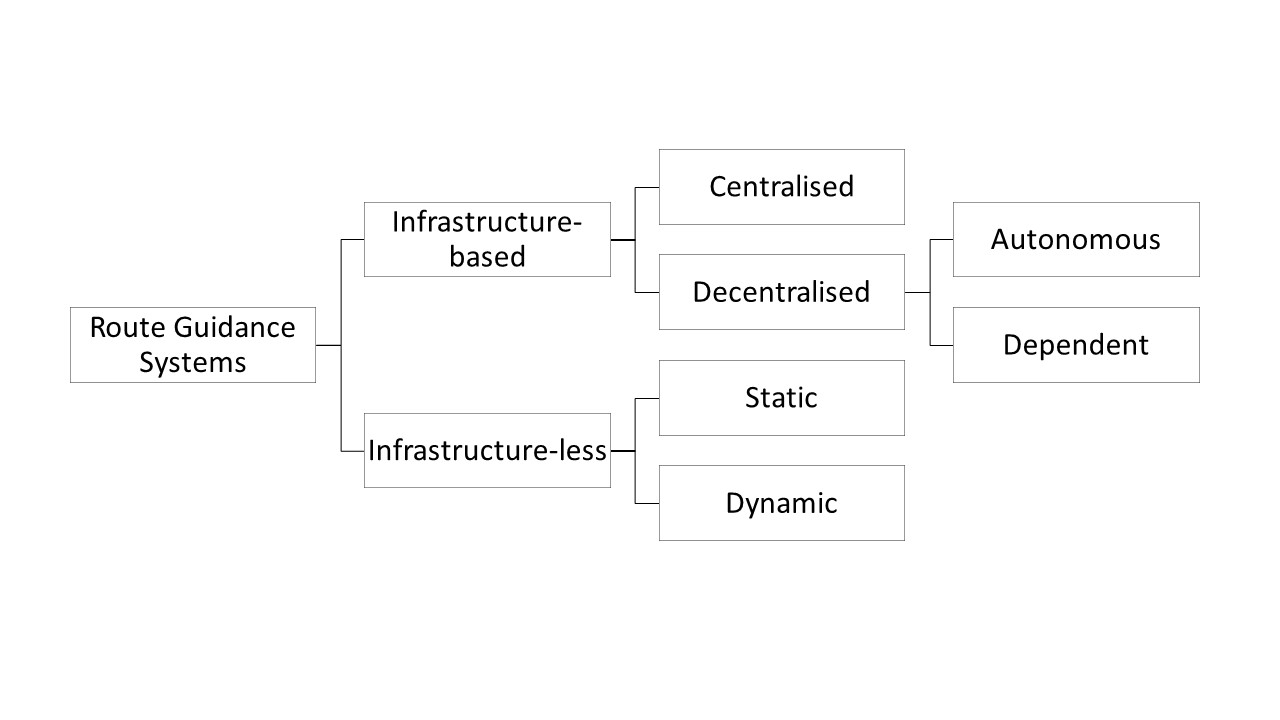
\includegraphics[width=0.55\linewidth]{image/DRS} \caption{Classification of route guidance systems (Khanjary and Hashemi, 2012)}\label{fig:unnamed-chunk-15}
\end{figure}

\textbf{Infrastrukturbasierte Architektur}
Sowohl bei \emph{zentralisierten infrastrukturbasierten Systemen} als auch bei \emph{dezentralisierten infrastrukturbasierten Systemen} werden die Daten zunächst von Verkehrserkennungssystemen erfasst und dann von Traffic Message Channel (TMC) gesammelt und extrahiert. Der Unterschied besteht darin, dass in einem \emph{zentralisierten System } die optimale Routeninformation für das gesamte Verkehrsnetz berechnet wird. Im Gegensatz dazu wird in einem \emph{abhängigen dezentralen System } die optimale Route für jedes Fahrzeug in Abhängigkeit von seinem aktuellen Standort und seinem Ziel berechnet. In einem \emph{vollständig automatisierten dezentralen System} werden die Daten von Straßenknoten gesammelt, die über das gesamte Verkehrsnetz verteilt sind und nützliche Informationen für alle umliegenden Straßen extrahieren und untereinander austauschen. Auf diese Weise kann jeder Knoten die optimalen Routen für verschiedene Ziele berechnen. Die Informationen über optimale Routen können von Fahrzeugen, Mobiltelefonen oder Wechselverkehrszeichen empfangen werden (Khanjary und Hashemi, 2012)

\textbf{Infrastrukturlose Architektur}
Das \emph{infrastrukturlose dezentrale statische System } ist eine der frühesten Entwicklungen. Die Datenbank mit der Karte des Verkehrsnetzes ist auf dem Mobiltelefon oder als fahrzeuginterne Einheit verfügbar, wobei die optimale Route auf der Grundlage statischer Informationen wie dem kürzesten Weg berechnet wird. In einem\emph{dezentralen dynamischen System }, werden Fahrzeuge (oder Mobiltelefone) zur Erfassung von Verkehrsdaten eingesetzt. Sie tauschen die Informationen untereinander über ein infrastrukturloses Protokoll wie die Kommunikation zwischen den Fahrzeugen oder Peer-to-Peer aus. Dies führt dazu, dass die Fahrzeuge über Echtzeit-Verkehrsinformationen über das gesamte Verkehrsnetz verfügen, die es ihnen ermöglichen, die optimale Route auf der Grundlage eines Ziels und der aktuellen Position des Fahrzeugs zu berechnen. Wichtig ist, dass die Genauigkeit des dynamischen Systems von der Anzahl der Fahrzeuge (oder mobilen Geräte) abhängt, die als Verkehrsdatensensoren dienen. Je mehr Fahrzeuge vorhanden sind, desto mehr Informationen können ausgetauscht werden und desto zuverlässiger sind die Daten (Khanjary und Hashemi, 2012).

\hypertarget{wichtige-interessensgruppen-13}{%
\subsection*{Wichtige Interessensgruppen}\label{wichtige-interessensgruppen-13}}
\addcontentsline{toc}{subsection}{Wichtige Interessensgruppen}

\begin{itemize}
\tightlist
\item
  \textbf{Betroffene}: Fahrer:innen
\item
  \textbf{Verantwortliche}: Lokale Regierungen, lokale oder nationale Straßeninfrastrukturanbieter, Automobilhersteller
\end{itemize}

\hypertarget{aktueller-stand-der-wissenschaft-und-forschung-13}{%
\subsection*{Aktueller Stand der Wissenschaft und Forschung}\label{aktueller-stand-der-wissenschaft-und-forschung-13}}
\addcontentsline{toc}{subsection}{Aktueller Stand der Wissenschaft und Forschung}

DRG ist bereits eine ausgereifte Technologie, daher konzentriert sich der Großteil der Forschung auf die Verbesserung verschiedener Aspekte oder die Anwendung in neuen Kontexten. In einer von Liang und Wakahara (2014) durchgeführten Studie werden beispielsweise Modelle zur Vorhersage des Stadtverkehrs vorgestellt, um ein zentrales proaktives Routenführungssystem zu schaffen. Die Ergebnisse zeigten, dass die Modelle den Vorhersagefehler verringerten und die Reisezeit verkürzten. Darüber hinaus schlugen Wang und Niu (2019) in ihrer Forschung eine simulationsbasierte verteilte dynamische Routenführung (DDRGS - Distributed Dynamic Route Guidance System) vor, die auf der Verwendung von Datenerfassungs- und Kommunikationstechniken in kooperativen Fahrzeug-Infrastruktur-Systemen (CVIS) basiert, und sie erklärten, dass die erstellte DDRGS in CVIS verwendet werden könnte. Deflorio (2003) bewertete die Leistung der Strategie zur Steuerung von DRG-Systemen in Experimenten unter der Bedingung eines schnellen Verkehrswachstums. Abschließend stellte Deflorio unter anderem fest, dass die durchschnittliche Reisezeit der DRG-Nutzer:innen in jedem untersuchten Fall kürzer war als die der Nicht-Nutzer:innen. Darüber hinaus befasst sich ein großer Teil der Forschung mit dem Einsatz von DRG im Zusammenhang mit vollständig automatisierten Fahrzeugen. In einer Studie von Lazar et al.~(2019) wird beispielsweise ein Deep Reinforcement Learning-Ansatz verwendet, um Staus im gemischten automatisierten Verkehr zu verringern. Darüber hinaus untersuchen Kaminski et al.~(2020) die Auswirkungen einer Änderung des Verbreitungsgrads von intelligenten Fahrzeugen auf die Systemeigenschaften, einschließlich der Reisezeit, in einer Umgebung, in der sowohl intelligente Fahrzeuge als auch von Menschen gesteuerte Fahrzeuge vorhanden sind. Dabei wird davon ausgegangen, dass intelligente Fahrzeuge auf Veränderungen im aktuell beobachteten Verkehr mit einer Umleitung reagieren, während herkömmliche Fahrzeuge nur auf historische Informationen zurückgreifen. Die Ergebnisse zeigen, dass der Umleitungsalgorithmus für intelligente Fahrzeuge die Gesamtreisezeit um bis zu 30\% verkürzt.

\hypertarget{aktueller-stand-der-praktischen-umsetzung-13}{%
\subsection*{Aktueller Stand der praktischen Umsetzung}\label{aktueller-stand-der-praktischen-umsetzung-13}}
\addcontentsline{toc}{subsection}{Aktueller Stand der praktischen Umsetzung}

Heutzutage nutzen Fahrer:innen verschiedener Automarken das Dynamic Route Guidance System bereits im Rahmen der dynamischen Navigation in der Fahrzeugausstattung. Seat (2012) bietet diese Funktion in der Navi-Satellitennavigationssoftware an. Seat gibt in seinem Handbuch für Autobesitzer an, dass die dynamische Routenführung auf dem TMC-Bericht basiert und die Rundfunkanstalten für diese Funktion verantwortlich sind (Media System Plus/ Navi System Owner's manual, 2012). Eine ähnliche Technologie wird auch von Volkswagen verwendet (Volkswagen, 2021). Eines der beliebtesten Tools zur Routenführung ist jedoch Google Maps, das dynamische Karten zur Verfügung stellt und Echtzeitdaten aus verschiedenen Kanälen verwendet, um die Karten so aktuell wie möglich zu halten (Custom Maps \textbar{} Google Maps Platform \textbar{} Google Cloud, 2021). Die Palette der von Google Maps angebotenen Funktionen wächst ständig. Kürzlich wurde über die reine dynamische Routenführung hinaus die Funktion ``Parkplatzsuche'' eingeführt (Vielmeier, 2019). Darüber hinaus spielt die dynamische Routenplanung eine wichtige Rolle im gewerblichen Verkehr und bei städtischen Lieferungen (PTVGroup.com, 2021).

\hypertarget{relevante-initiativen-in-uxf6sterreich-13}{%
\subsection*{Relevante Initiativen in Österreich}\label{relevante-initiativen-in-uxf6sterreich-13}}
\addcontentsline{toc}{subsection}{Relevante Initiativen in Österreich}

\begin{itemize}
\tightlist
\item
  \href{https://www.volkswagen.at/technik-lexikon/navigationssystem}{Volkswagen}
\item
  \href{https://blog.ptvgroup.com/de/stadt-und-mobilitaet/routing-engine-hyperpath/}{PTVGroup}
\item
  \href{https://www.capterra.at/directory/30944/route-planning/software}{Capterra.at}
\end{itemize}

\hypertarget{auswirkungen-in-bezug-auf-die-ziele-fuxfcr-nachhaltige-entwicklung-sdgs-13}{%
\subsection*{Auswirkungen in Bezug auf die Ziele für nachhaltige Entwicklung (SDGs)}\label{auswirkungen-in-bezug-auf-die-ziele-fuxfcr-nachhaltige-entwicklung-sdgs-13}}
\addcontentsline{toc}{subsection}{Auswirkungen in Bezug auf die Ziele für nachhaltige Entwicklung (SDGs)}

\begin{longtable}[]{@{}ccccc@{}}
\toprule
\begin{minipage}[b]{0.17\columnwidth}\centering
Ebene der Auswirkungen\strut
\end{minipage} & \begin{minipage}[b]{0.16\columnwidth}\centering
Indikator\strut
\end{minipage} & \begin{minipage}[b]{0.17\columnwidth}\centering
Richtung der Auswirkungen\strut
\end{minipage} & \begin{minipage}[b]{0.17\columnwidth}\centering
Beschreibung des Ziels \& SDG\strut
\end{minipage} & \begin{minipage}[b]{0.17\columnwidth}\centering
Quelle\strut
\end{minipage}\tabularnewline
\midrule
\endhead
\begin{minipage}[t]{0.17\columnwidth}\centering
Individuell\strut
\end{minipage} & \begin{minipage}[t]{0.16\columnwidth}\centering
Verkuerzte Reisezeit\strut
\end{minipage} & \begin{minipage}[t]{0.17\columnwidth}\centering
\textbf{+}\strut
\end{minipage} & \begin{minipage}[t]{0.17\columnwidth}\centering
Nachhaltige wirtschaftliche Entwicklung (\emph{8,11})\strut
\end{minipage} & \begin{minipage}[t]{0.17\columnwidth}\centering
Deflorio, 2003\strut
\end{minipage}\tabularnewline
\begin{minipage}[t]{0.17\columnwidth}\centering
Systemisch\strut
\end{minipage} & \begin{minipage}[t]{0.16\columnwidth}\centering
Geringeres Unfallrisiko durch Routenwechsel\strut
\end{minipage} & \begin{minipage}[t]{0.17\columnwidth}\centering
\textbf{+}\strut
\end{minipage} & \begin{minipage}[t]{0.17\columnwidth}\centering
Gesundheit und Wohlbefinden (\emph{3})\strut
\end{minipage} & \begin{minipage}[t]{0.17\columnwidth}\centering
Chatterjee and McDonald, 1999\strut
\end{minipage}\tabularnewline
\bottomrule
\end{longtable}

\hypertarget{technologie--und-gesellschaftlicher-bereitschaftsgrad-11}{%
\subsection*{Technologie- und gesellschaftlicher Bereitschaftsgrad}\label{technologie--und-gesellschaftlicher-bereitschaftsgrad-11}}
\addcontentsline{toc}{subsection}{Technologie- und gesellschaftlicher Bereitschaftsgrad}

\begin{longtable}[]{@{}cc@{}}
\toprule
Stand der Technologiebereitschaft & Gesellschaftlicher Bereitschaftsgrad\tabularnewline
\midrule
\endhead
7-9 & 8-9\tabularnewline
\bottomrule
\end{longtable}

\hypertarget{offene-fragen-13}{%
\subsection*{Offene Fragen}\label{offene-fragen-13}}
\addcontentsline{toc}{subsection}{Offene Fragen}

\begin{enumerate}
\def\labelenumi{\arabic{enumi}.}
\tightlist
\item
  Wie kann die zeitliche Genauigkeit und generell die Leistung der dynamischen Routenführung durch Verkehrsfunkkanäle verbessert werden?
\item
  Wirkt sich die dynamische Routenführung auf die Sicherheit der Fahrer:innen aus und wenn ja, in welchem Maße?
\item
  Was sind die Grenzen und welche Risiken könnten durch die dynamische Routenführung möglicherweise vermieden werden?
\item
  Wie ist die Anwendbarkeit von DRG für vollständig automatisierte Fahrzeuge?
\end{enumerate}

\hypertarget{weitere-links-11}{%
\subsection*{Weitere links}\label{weitere-links-11}}
\addcontentsline{toc}{subsection}{Weitere links}

\begin{itemize}
\tightlist
\item
  \href{https://www.verizonconnect.com/at/industrie/vertriebsroutenplaner/}{Verizonconnect.com}
\end{itemize}

\hypertarget{referenzen-13}{%
\subsection*{Referenzen}\label{referenzen-13}}
\addcontentsline{toc}{subsection}{Referenzen}

\begin{itemize}
\tightlist
\item
  Chatterjee, K. and McDonald, M., (1999). THE NETWORK SAFETY EFFECTS OF DYNAMIC ROUTE GUIDANCE. ITS Journal - Intelligent Transportation Systems Journal, 4(3-4), pp.258-260.
\item
  Blischke, F., \& Hessing, B. (1998). Dynamic Route Guidance - Different Approaches to the System Concepts. SAE Transactions, 107, 1107-1111. Available at: \url{http://www.jstor.org/stable/44741041} {[}Accessed: 22 July 2021{]}
\item
  Deflorio, F., (2003). Evaluation of a reactive dynamic route guidance strategy. Transportation Research Part C: Emerging Technologies, 11(5), pp.375-388.
\item
  European Commission. (2021). Traveller Information - Mobility and Transport - European Commission. Available at: \url{https://ec.europa.eu/transport/themes/its/road/application_areas/traveller_information_es} {[}Accessed: 23 July 2021{]}.
\item
  Fan, Y., Lu, D., Li, Y. and Jiang, F., (2010). Design scheme of Distributed Dynamic Route Guidance System. 2010 2nd International Conference on Education Technology and Computer.
\item
  Google Cloud. (2021). Custom Maps \textbar{} Google Maps Platform \textbar{} Google Cloud. Available at: \url{https://cloud.google.com/maps-platform/maps} {[}Accessed: 23 July 2021{]}.
\item
  Kaminski, B., Krainski, A., Mashatan, A., Pralat, P., \& Szufel, P. (2020). Multiagent Routing Simulation with Partial Smart Vehicles Penetration. Journal of Advanced Transportation, 2020.
\item
  Khanjary, M., \& Hashemi, S. M. (2012, May). Route guidance systems: Review and classification. In 2012 6th Euro American Conference on Telematics and Information Systems (EATIS) (pp.~1-7). IEEE.
\item
  Lazar, D. A., Biyik, E., Sadigh, D., \& Pedarsani, R. (2021). Learning how to dynamically route autonomous vehicles on shared roads. Transportation Research Part C: Emerging Technologies, 130, 103258.
\item
  Liang, Z. and Wakahara, Y., (2014). Real-time urban traffic amount prediction models for dynamic route guidance systems. EURASIP Journal on Wireless Communications and Networking, 2014(1).
\item
  Media System Plus. (2012). Media System Plus/ Navi System Owner's manual. Available at: \url{https://www.firstforseatcars.com/downloads/multimedia/media-system-plus-navi-system-owners-manual.pdf} {[}Accessed: 22 July 2021{]}.
\item
  Mobility and transport. (2021). Intelligent transport systems Traveller Information. Available at: \url{https://ec.europa.eu/transport/themes/its/road/application_areas/traveller_information_es} {[}Accessed: 22 July 2021{]}.
\item
  Park, D., Kim, H., Lee, C. and Lee, K., (2009). Location-based dynamic route guidance system of Korea: System design, algorithms and initial results. KSCE Journal of Civil Engineering, 14(1), pp.51-59.
\item
  PTVGroup.com (2021). PTV Map\&Guide - der weltweit führende Lkw Routenplaner mit Transportkosten- und Mautrechner. Available at: \url{https://www.ptvgroup.com/de/loesungen/produkte/ptv-mapandguide/} {[}Accessed: 28 July 2021{]}
\item
  Seat.com. (2021). Dynamic Route Guidance - Car Terms \textbar{} SEAT. Available at: \url{https://www.seat.com/car-terms/d/dynaminc-route-guidance.html} {[}Accessed: 23 July 2021{]}.
\item
  Wang, J. and Niu, H., (2019). A distributed dynamic route guidance approach based on short-term forecasts in cooperative infrastructure-vehicle systems. Transportation Research Part D: Transport and Environment, 66, pp.23-34.
\item
  Vielmeier J. (2019). Google Maps als Navi verwenden: Das müsst ihr beachten. Available at: \url{https://trendblog.euronics.de/mobile-web/google-maps-als-navi-verwenden-das-muesst-ihr-beachten-61614/}. {[}Accessed: 28 July 2021{]}
\item
  Volkswagen.at (2021) Navigation. Volkswagen Technik-Highlights. Available at: \url{https://www.volkswagen.at/technik-lexikon/navigationssystem} {[}Accessed: 28 July 2021{]}.
\end{itemize}

\hypertarget{variable_speed}{%
\section{Variable Geschwindigkeitsbegrenzungen und dynamisches Beschilderungssystem}\label{variable_speed}}

\hypertarget{synonyme-13}{%
\subsection*{Synonyme}\label{synonyme-13}}
\addcontentsline{toc}{subsection}{Synonyme}

\emph{Variable Geschwindigkeitsbegrenzungen (VSL - Variable speed limits), dynamische Geschwindigkeitsbegrenzungen (DSL - dynamic speed limits), Verkehrsbeeinflussungsanlagen (VBA), Wechselverkehrszeichen (CMS - Changeable Message Signs), Dynamisches Beschilderungssystem, \href{http://changemobility.at/wiki/index.php?title=Regularien\#Geschwindigkeitsbegrenzungen}{Geschwindigkeitsbegrenzungen}}

\hypertarget{definition-14}{%
\subsection*{Definition}\label{definition-14}}
\addcontentsline{toc}{subsection}{Definition}

Geschwindigkeitsbegrenzungen beruhen auf Sicherheits-, Mobilitäts- und Umwelterwägungen. Während feste Geschwindigkeitsbegrenzungen die angemessene Geschwindigkeit für durchschnittliche Bedingungen darstellen, berücksichtigen variable oder dynamische Geschwindigkeitsbegrenzungen (DSL) den Verkehr in Echtzeit oder die Straßen- und Wetterbedingungen. Letztere spiegeln daher die sichere Geschwindigkeit besser wider (Mobilität und Verkehr, 2020). Die Verkehrsteilnehmer:innen werden in der Regel durch elektronische Schilder über oder neben den Fahrspuren über das aktuelle Tempolimit informiert (De Pauw et al., 2018), wie in Abbildung 1 dargestellt. Diese können durch Warnschilder ergänzt werden (dynamisches Beschilderungssystem). Wenn beispielsweise die übliche Höchstgeschwindigkeit 100 km/h beträgt, könnte das DSL auf 80 km/h und weiter auf 60 km/h geändert werden, um Auffahrunfälle zu vermeiden, wenn z. B. ein Stau vorausgeht oder die Wetterbedingungen schwierig sind.

\begin{figure}
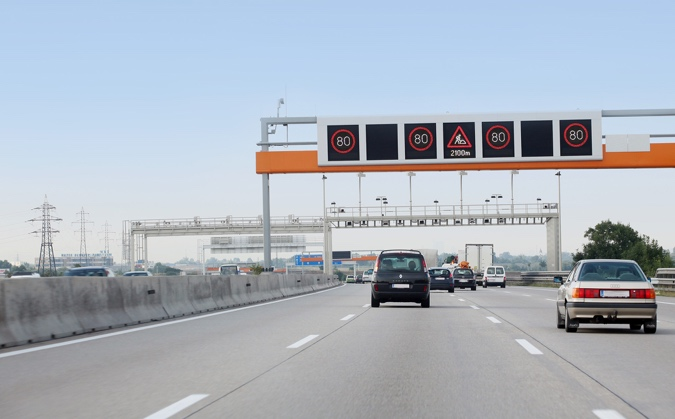
\includegraphics[width=0.9\linewidth]{image/dynamic_signage} \caption{Dynamisches Beschilderungssystem in Oesterreich (ASFiNAG, 2019b)}\label{fig:unnamed-chunk-18}
\end{figure}

Was die Auswirkungen auf die gesellschaftliche Ebene betrifft, so zeigte eine belgische Studie von E. De Pauw et al.~einen signifikanten Rückgang (-18 \%) der Zahl der Unfälle mit Verletzten nach der Einführung eines DSL-Systems (De Pauw et al., 2018). F.G. Habtemichael und L. de Picado Santos (2013) fanden heraus, dass ein DSL-System den höchsten Sicherheitsnutzen bei stark überlasteten Verkehrsbedingungen hat. Der betriebliche Nutzen wiederum war bei leicht überlasteten Verkehrsbedingungen am höchsten. Der Erfolg von DSL hängt jedoch in hohem Maße von der Einhaltung der Vorschriften durch die Fahrer:innen ab (Habtemichael \& de Picado Santos, 2013). Neben den Sicherheitsaspekten besteht das Ziel von DSL darin, den Verkehrsfluss zu harmonisieren. Starker Verkehr kann Stoßwellen verursachen, die zu längeren Fahrzeiten und großen Geschwindigkeitsschwankungen zwischen den Fahrzeugen führen. Letzteres kann wiederum zu unsicheren Situationen führen. Durch den Einsatz von DSL könnte dieses Phänomen verringert werden (Hegyi et al., 2005). Die Effizienz des Verkehrsflusses kann noch weiter verbessert werden, wenn DSL mit einer koordinierten Rampenzählung kombiniert wird (Carlson, 2010). Geschwindigkeitsbegrenzungen können auch aufgrund hoher Emissionswerte vorübergehend herabgesetzt werden. Wenn die Emissionswerte in Kombination mit dem Verkehrsaufkommen einen bestimmten Wert erreichen, reagiert das DSL-System automatisch und senkt die Geschwindigkeitsbegrenzung für eine bestimmte Zeit. Wie hoch dieses Niveau ist, hängt von den lokalen Richtlinien ab (ASFiNAG, 2019c).

\hypertarget{wichtige-interessensgruppen-14}{%
\subsection*{Wichtige Interessensgruppen}\label{wichtige-interessensgruppen-14}}
\addcontentsline{toc}{subsection}{Wichtige Interessensgruppen}

\begin{itemize}
\tightlist
\item
  \textbf{Betroffene}: Benutzer:innen von Autobahnen, Fahrer:innen
\item
  \textbf{Verantwortliche}: Autobahninfrastruktur-Agenturen, Technologie-Anbieter, politische Entscheidungsträger:innen, staatliche Behörden
\end{itemize}

\hypertarget{aktueller-stand-der-wissenschaft-und-forschung-14}{%
\subsection*{Aktueller Stand der Wissenschaft und Forschung}\label{aktueller-stand-der-wissenschaft-und-forschung-14}}
\addcontentsline{toc}{subsection}{Aktueller Stand der Wissenschaft und Forschung}

Studien zeigen, dass die meisten DSL-Einführungen in Europa rückblickend die Verkehrssicherheit und den Verkehrsfluss effizient verbessert haben. In den Vereinigten Staaten war die Erhöhung der Sicherheit ebenfalls signifikant, aber die Verbesserung des Verkehrsflusses war umstritten (Lu \& Shladover, 2014). Hassan et al.~(2012) fanden heraus, dass bei schlechten Wetterbedingungen die Kombination von Wechselverkehrszeichen (CMS) und DSL die beste Möglichkeit zur Verbesserung der Sicherheit war. Aktuelle Forschungen zeigen, dass die Vorteile von DSL-Systemen durch die Integration in eine vollständig vernetzte Fahrzeugumgebung (Wu et al., 2020) verbessert werden könnten. Derzeit konzentriert sich die Forschung auf die Integration von C-ITS, um die Infrastruktur mit den Fahrzeugen zu verbinden. In den nächsten Jahren sollten europäische Normen entwickelt werden (Erhart, 2019).

\hypertarget{aktueller-stand-der-praktischen-umsetzung-14}{%
\subsection*{Aktueller Stand der praktischen Umsetzung}\label{aktueller-stand-der-praktischen-umsetzung-14}}
\addcontentsline{toc}{subsection}{Aktueller Stand der praktischen Umsetzung}

DSL-Systeme werden auf der ganzen Welt eingeführt und verwendet. Die verwendeten Algorithmen unterscheiden sich jedoch. DSL integriert mit C-ITS wurde in einer Testumgebung implementiert (Erhart, 2019). Die österreichischen Autobahnen werden von der ASFiNAG verwaltet - derzeit sind dort 17 DSL-Systeme im Einsatz. Das bedeutet, dass etwa 19 \% des österreichischen Autobahnnetzes derzeit mit einem DSL-System ausgestattet sind (ASFiNAG, 2019a). Es gibt also noch Ausbaupotenzial. Ein Global Player im Verkehrsmanagement ist das österreichische Unternehmen Kapsch TrafficCom. Weltweit haben sie ihre Systeme auf mehr als 3.500 km Autobahn implementiert (Kapsch TrefficCom). Die rund 5.000 Mitarbeiter:innen von Kapsch TrafficCom erwirtschafteten im Wirtschaftsjahr 2018/19 einen Umsatz von 738 Millionen Euro.

\hypertarget{relevante-initiativen-in-uxf6sterreich-14}{%
\subsection*{Relevante Initiativen in Österreich}\label{relevante-initiativen-in-uxf6sterreich-14}}
\addcontentsline{toc}{subsection}{Relevante Initiativen in Österreich}

\begin{itemize}
\tightlist
\item
  \href{https://www.asfinag.at/verkehrssicherheit/verkehrsmanagement/verkehrssteuerung/}{Asfinag}
\item
  \href{https://blog.asfinag.at/technik-innovation/c-its-vernetzte-autos-intelligenter-verkehr/}{Asifinag blog}
\item
  \href{https://www.kapsch.net/ktc/Portfolio/IMS/Congestion/Highway-Traffic-Management}{kapsch.net}
\item
  \href{https://www.strabag-iss.com/databases/internet/_public/content30.nsf/web30?Openagent\&id=DE-STRABAGISS-DE_verkehrstechnik.html\&men1=3\&men2=5\&sid=351}{strabag-iss.com}
\item
  \href{https://www.pke.at/index.php?id=17\#c117}{pke.at}
\item
  \href{http://www.aigner-stahlbau.at/leistungen/verkehrstechnik/}{aigner-stahlbau.at}
\end{itemize}

\hypertarget{auswirkungen-in-bezug-auf-die-ziele-fuxfcr-nachhaltige-entwicklung-sdgs-14}{%
\subsection*{Auswirkungen in Bezug auf die Ziele für nachhaltige Entwicklung (SDGs)}\label{auswirkungen-in-bezug-auf-die-ziele-fuxfcr-nachhaltige-entwicklung-sdgs-14}}
\addcontentsline{toc}{subsection}{Auswirkungen in Bezug auf die Ziele für nachhaltige Entwicklung (SDGs)}

\begin{longtable}[]{@{}ccccc@{}}
\toprule
\begin{minipage}[b]{0.17\columnwidth}\centering
Ebene der Auswirkungen\strut
\end{minipage} & \begin{minipage}[b]{0.16\columnwidth}\centering
Indikator\strut
\end{minipage} & \begin{minipage}[b]{0.17\columnwidth}\centering
Richtung der Auswirkungen\strut
\end{minipage} & \begin{minipage}[b]{0.17\columnwidth}\centering
Beschreibung des Ziels \& SDG\strut
\end{minipage} & \begin{minipage}[b]{0.17\columnwidth}\centering
Quelle\strut
\end{minipage}\tabularnewline
\midrule
\endhead
\begin{minipage}[t]{0.17\columnwidth}\centering
Individuell\strut
\end{minipage} & \begin{minipage}[t]{0.16\columnwidth}\centering
Toedliche Kollisionen reduziert\strut
\end{minipage} & \begin{minipage}[t]{0.17\columnwidth}\centering
\textbf{+}\strut
\end{minipage} & \begin{minipage}[t]{0.17\columnwidth}\centering
Gesundheit und Wohlbefinden (\emph{3})\strut
\end{minipage} & \begin{minipage}[t]{0.17\columnwidth}\centering
Hegyi et al., 2005\strut
\end{minipage}\tabularnewline
\begin{minipage}[t]{0.17\columnwidth}\centering
Individuell\strut
\end{minipage} & \begin{minipage}[t]{0.16\columnwidth}\centering
Verkuerzte Reisezeit\strut
\end{minipage} & \begin{minipage}[t]{0.17\columnwidth}\centering
\textbf{+}\strut
\end{minipage} & \begin{minipage}[t]{0.17\columnwidth}\centering
Nachhaltige wirtschaftliche Entwicklung (\emph{8,11})\strut
\end{minipage} & \begin{minipage}[t]{0.17\columnwidth}\centering
Habtemichael \& de Picado Santos, 2013\strut
\end{minipage}\tabularnewline
\begin{minipage}[t]{0.17\columnwidth}\centering
Systemisch\strut
\end{minipage} & \begin{minipage}[t]{0.16\columnwidth}\centering
Toedliche Kollisionen reduziert\strut
\end{minipage} & \begin{minipage}[t]{0.17\columnwidth}\centering
\textbf{+}\strut
\end{minipage} & \begin{minipage}[t]{0.17\columnwidth}\centering
Gesundheit und Wohlbefinden (\emph{3})\strut
\end{minipage} & \begin{minipage}[t]{0.17\columnwidth}\centering
Hegyi et al., 2005\strut
\end{minipage}\tabularnewline
\begin{minipage}[t]{0.17\columnwidth}\centering
Systemisch\strut
\end{minipage} & \begin{minipage}[t]{0.16\columnwidth}\centering
Jaehrlicher Rueckgang der Treibhausgasemissionen\strut
\end{minipage} & \begin{minipage}[t]{0.17\columnwidth}\centering
\textbf{+}\strut
\end{minipage} & \begin{minipage}[t]{0.17\columnwidth}\centering
Oekologische Nachhaltigkeit (\emph{7,12-13,15})\strut
\end{minipage} & \begin{minipage}[t]{0.17\columnwidth}\centering
Schimany, 2011\strut
\end{minipage}\tabularnewline
\bottomrule
\end{longtable}

\hypertarget{technologie--und-gesellschaftlicher-bereitschaftsgrad-12}{%
\subsection*{Technologie- und gesellschaftlicher Bereitschaftsgrad}\label{technologie--und-gesellschaftlicher-bereitschaftsgrad-12}}
\addcontentsline{toc}{subsection}{Technologie- und gesellschaftlicher Bereitschaftsgrad}

\begin{longtable}[]{@{}cc@{}}
\toprule
Stand der Technologiebereitschaft & Gesellschaftlicher Bereitschaftsgrad\tabularnewline
\midrule
\endhead
7-9 & 8-9\tabularnewline
\bottomrule
\end{longtable}

\hypertarget{offene-fragen-14}{%
\subsection*{Offene Fragen}\label{offene-fragen-14}}
\addcontentsline{toc}{subsection}{Offene Fragen}

\begin{enumerate}
\def\labelenumi{\arabic{enumi}.}
\tightlist
\item
  Welche Algorithmen für DSL sind die effizientesten?
\item
  Wie kann DSL weiter entwickelt werden?
\item
  Wie kann der ausfallsichere Betrieb verbessert werden?
\item
  Wie kann DSL mit C-ITS kombiniert werden?
\end{enumerate}

\hypertarget{referenzen-14}{%
\subsection*{Referenzen}\label{referenzen-14}}
\addcontentsline{toc}{subsection}{Referenzen}

\begin{itemize}
\tightlist
\item
  ASFiNAG. (2019a). Handlungsfelder. Available at: \url{http://verkehrssicherheit.asfinag.at/aktionsprogramme/handlungsfelder/} {[}Accessed: 17 December 2020{]}.
\item
  ASFiNAG. (2019b). Verkehrsbeeinflussungsanlagen - Für mehr Sicherheit: Arten von Verkehrsbeeinflussungsanlagen. Available at: \url{https://asfinag.azureedge.net/media/1607/vba-fotomontage.jpg} {[}Accessed: 11 December 2020{]}.
\item
  ASFiNAG. (2019c). Verkehrsbeeinflussungsanlagen - Für mehr Sicherheit: Die VBA und der ``Lufthunderter''. Available at: \url{https://www.asfinag.at/verkehrssicherheit/verkehrsmanagement/verkehrssteuerung/} {[}Accessed: 3 December 2020{]}.
\item
  Carlson, R. C., Papamichail, I., Papageorgiou, M., \& Messmer, A. (2010). Optimal motorway traffic flow control involving variable speed limits and ramp metering. Transportation Science, 44(2), 238-253.
\item
  De Pauw, E., Daniels, S., Franckx, L., \& Mayeres, I. (2018). Safety effects of dynamic speed limits on motorways. Accident Analysis \& Prevention, 114, 83-89.
\item
  Erhart, Jaqueline. (2019). Vernetzte Autos, intelligenter Verkehr: Was C-ITS ist, was es kann und wem es nutzt. Available at: \url{https://blog.asfinag.at/technik-innovation/c-its-vernetzte-autos-intelligenter-verkehr/} {[}Accessed: 17 December 2020{]}.
\item
  Habtemichael, F. G., \& de Picado Santos, L. (2013). Safety and Operational Benefits of Variable Speed Limits under Different Traffic Conditions and Driver Compliance Levels. Transportation Research Record, 2386(1), 7-15. \url{https://doi.org/10.3141/2386-02}
\item
  Hassan, H. M., Abdel-Aty, M. A., Choi, K., \& Algadhi, S. A. (2012). Driver behavior and preferences for changeable message signs and variable speed limits in reduced visibility conditions. Journal of Intelligent Transportation Systems, 16(3), 132-146.
\item
  Hegyi, A., De Schutter, B., \& Hellendoorn, J. (2005). Optimal coordination of variable speed limits to suppress shock waves. IEEE Transactions on intelligent transportation systems, 6(1), 102-112.
\item
  Kapsch TrefficCom. Verkehrsmanagement auf Autobahnen. Available at: \url{https://www.kapsch.net/ktc/Portfolio/IMS/Congestion/Highway-Traffic-Management}
\item
  Lu, X.-Y., \& Shladover, S. E. (2014). Review of Variable Speed Limits and Advisories: Theory, Algorithms, and Practice. Transportation Research Record, 2423(1), 15-23. \url{https://doi.org/10.3141/2423-03} {[}Accessed: 8 January 2021{]}
\item
  Mobility and Transport \textbar{} European Commission. (2020). Dynamic speed limits. Available at: \url{https://ec.europa.eu/transport/road_safety/specialist/knowledge/speed/new_technologies_new_opportunities/dynamic_speed_limits_en} {[}Accessed: 2 December 2020{]}.
\item
  Schimany, H. K. (2011). Blue Globe Foresight.
\item
  Wu, Y., Abdel-Aty, M., Wang, L., \& Rahman, M. S. (2020). Combined connected vehicles and variable speed limit strategies to reduce rear-end crash risk under fog conditions. Journal of Intelligent Transportation Systems, 24(5), 494-513.
\end{itemize}

\hypertarget{adaptive_traffic_control}{%
\section{Intelligente Verkehrssignalsteuerung}\label{adaptive_traffic_control}}

\hypertarget{synonyme-14}{%
\subsection*{Synonyme}\label{synonyme-14}}
\addcontentsline{toc}{subsection}{Synonyme}

\emph{Intelligente Ampelanlagen, adaptive Verkehrssignalsteuerung (ATSC - Adaptive Traffic Signal Control), Verkehrssignalsteuerung (TST - Traffic Signal Timing), Verkehrssignalsteuerung (TSC - Traffic Signal Control)}

\hypertarget{definition-15}{%
\subsection*{Definition}\label{definition-15}}
\addcontentsline{toc}{subsection}{Definition}

In den letzten Jahren haben die steigende Bevölkerungszahl und der dringende Bedarf an effizientem Verkehr zu schwerwiegenden Verkehrsproblemen geführt, insbesondere in städtischen Gebieten. Es wurden Lösungen zur Stauabschwächung vorgeschlagen, wie z. B. die Optimierung des Straßennetzes und die Verbesserung grundlegender städtischer Verwaltungseinrichtungen, um den durch die großen Verkehrsströme während der Spitzenzeiten verursachten Druck zu bewältigen. Unter allen möglichen Methoden hat sich die adaptive Verkehrssignalsteuerung (ATSC), bei der die Intelligenz in die Ampelsteuerungssysteme integriert wird, als wirtschaftlich und effizient erwiesen, um den Verkehrsdruck an überlasteten Kreuzungen zu verringern. Mit der Entwicklung von Deep-Learning-Techniken haben ATSC-Strategien großes Potenzial für die Integration modernster intelligenter Methoden gezeigt (Wang et al., 2021).
Bestehende Ampelsteuerungssysteme verwenden entweder feste Programme ohne Berücksichtigung des Echtzeitverkehrs oder berücksichtigen den Verkehr kaum (Casas, 2017). Sie stellen die Ampeln entweder in jedem Zyklus auf die gleiche Dauer ein oder variieren die Dauer in Abhängigkeit von historischen Informationen. Einige von ihnen verwenden Eingangsdaten von unterirdischen Sensoren, wie z. B. Induktionsschleifendetektoren, um Fahrzeuge in der Nähe der Ampel zu erkennen. Diese Daten werden jedoch nur sehr grob verarbeitet, um die Dauer von grünen und roten Ampeln zu bestimmen. Folglich funktionieren sie in einigen Fällen (mit geringer Effizienz); bei Ereignissen wie Sportveranstaltungen, Festivals, Wetterbedingungen oder einem typischen Szenario mit hohem Verkehrsaufkommen neigen die bestehenden Kontrollsysteme jedoch dazu, lahmgelegt zu werden.
In einer aktuellen Forschungsarbeit von Liang et al.~(2019) wird berichtet, dass erfahrene Polizeibeamt:innen eine Kreuzung effizient und direkt durch Winken kontrollieren können. Insbesondere in Szenarien mit hohem Verkehrsaufkommen beobachten menschliche Bediener:innen die Echtzeit-Verkehrsbedingungen an den kreuzenden Straßen und passen die Dauer der Durchfahrtszeit entsprechend an. Das Ziel der adaptiven Verkehrssignalsteuerung ist es, durch den Einsatz von V2X und Deep Reinforcement Learning (Wang et al., 2021) eine Flexibilität und Effizienz im Verkehrsmanagement zu erreichen, das mit dem von menschlichen Bediener:innen vergleichbar ist.

\hypertarget{wichtige-interessensgruppen-15}{%
\subsection*{Wichtige Interessensgruppen}\label{wichtige-interessensgruppen-15}}
\addcontentsline{toc}{subsection}{Wichtige Interessensgruppen}

\begin{itemize}
\tightlist
\item
  \textbf{Betroffene}: Autofahrer:innen, Radfahrer:innen, Fußgänger:innen
\item
  \textbf{Verantwortliche}: Lokale Regierungen, lokale oder nationale Straßeninfrastrukturanbieter, Automobilhersteller
\end{itemize}

\hypertarget{aktueller-stand-der-wissenschaft-und-forschung-15}{%
\subsection*{Aktueller Stand der Wissenschaft und Forschung}\label{aktueller-stand-der-wissenschaft-und-forschung-15}}
\addcontentsline{toc}{subsection}{Aktueller Stand der Wissenschaft und Forschung}

Bestehende ATSC-Methoden konzentrieren sich darauf, die Dauer von Grün- oder Rotphasen auf der Grundlage von Echtzeitinformationen zu variieren. Dieser Ansatz ist jedoch nicht optimal, da er die Auswirkungen der aktuellen Dauer der grünen und roten Ampeln auf den nachfolgenden Verkehr vernachlässigt. Daher schneidet ATSC besser ab als das System mit fester Dauer, aber schlechter als flexiblere Methoden, da die optimale Phasendauer in den letzten Zyklen unter Berücksichtigung aktueller Informationen über komplexe Verkehrsbedingungen in der Zukunft nicht besser ist.

Mit Deep Learning (DL)-Methoden (die als Input für die Kreuzungssteuerung dienen) kann die optimale Gestaltung der grundlegenden Steuerungsindizes wie Grünphasendauer und Phasenfolge der Ampel an einer Kreuzung als ein optimales Entscheidungsverfahren betrachtet werden. Anschließend wird das Reinforcement Learning (RL) auf die Signalsteuerung angewandt, um das beste Steuerungsverfahren für eine signalisierte Kreuzung zu finden. Um jedoch eine sofortige Datenerfassung und -übertragung mit geringer Latenzzeit zu erreichen, ist ein kooperatives Fahrzeuginfrastruktursystem (CVIS) erforderlich, das die Kommunikation zwischen den Fahrzeugen und zwischen Fahrzeugen und straßenseitiger Infrastruktur unterstützt (siehe \protect\hyperlink{v2x}{Abschnitt V2X}). Im Vergleich zu herkömmlichen Sensordetektoren kann V2X genauere Verkehrsdaten sammeln, um umfassende Informationen für die Verkehrssteuerung zu liefern, was zu besseren RL-Entscheidungen führt (Wang et al., 2021)
Darüber hinaus ergab die Analyse der neueren Literatur zur Optimierung von TSC-Systemen, die von Januar 2015 bis Januar 2020 veröffentlicht wurden, dass sich nur zwei Arbeiten mit signalisierten Kreisverkehren befassen. Kreisverkehre haben eine andere Verkehrsdynamik als reguläre Kreuzungen. Angesichts des zunehmenden Einsatzes von signalisierten Kreisverkehren, insbesondere in städtischen Gebieten, wird davon ausgegangen, dass TSC für signalisierte Kreisverkehre eine besondere Forschungslücke in diesem Bereich darstellt. Obwohl es Studien gibt, die mit realen Daten und Echtzeitsteuerung durchgeführt wurden, gibt es nur wenige Ergebnisse und/oder Methoden, die in der Praxis angewandt oder angepasst wurden. Eine der größten Herausforderungen für die Forscher:innen auf diesem Gebiet besteht darin, diese Methoden den Entscheidungsträger:innen und Umsetzer:innen näher zu bringen.
Darüber hinaus befasst sich die überwiegende Mehrheit der zu diesem Thema gefundenen Arbeiten mit der zeitlichen Steuerung von Verkehrssignalen und deren Auswirkungen auf die durchschnittliche Verspätung und/oder die Emissionen. Ein wichtiger Bestandteil von stark befahrenen Kreuzungen, insbesondere in Ballungsgebieten, ist der Fußgängerverkehr. Mit Ausnahme von Vilarinho et al., (2017) und Yu et al., (2017) werden Fußgänger:innen und die Auswirkungen ihres Verhaltens in den Studien nicht modelliert. Das Gleiche gilt für das Verhalten der Fahrer:innen. Eine wichtige Forschungsrichtung wäre es, die Auswirkungen des Fußgänger- und Fahrerverhaltens auf die Modelle zu analysieren.
Außerdem nimmt die Zahl der Studien, die sich mit automatisierten Fahrzeugen und Technologien befassen, rasch zu. Die jüngsten Studien befassen sich mit der allgemeinen Frage, wie vollständig automatisierte Fahrzeuge sicher und/oder effizient und/oder umweltfreundlich in den Verkehrsfluss eingeführt werden können (Qadri et al., 2020a).
Das Lernen durch Versuch und Irrtum ist zwar der Kerngedanke von RL, aber die Lernkosten von RL für komplizierte Probleme könnten inakzeptabel sein. Daher ist die Frage, wie man effizient lernt (z. B. aus begrenzten Datenproben, effiziente Exploration, Übertragung von gelerntem Wissen), ein entscheidender Punkt für die Anwendung von RL in der Verkehrssignalsteuerung (Wei et al., 2019).

\hypertarget{aktueller-stand-der-praktischen-umsetzung-15}{%
\subsection*{Aktueller Stand der praktischen Umsetzung}\label{aktueller-stand-der-praktischen-umsetzung-15}}
\addcontentsline{toc}{subsection}{Aktueller Stand der praktischen Umsetzung}

Eine Reihe von Akteuren konzentriert sich auf die Entwicklung adaptiver Verkehrssteuerungssysteme, die eine Reihe von Smart-City-Verkehrsanwendungen unterstützen, wie z. B. Signalpriorität für öffentliche Verkehrsmittel (siehe \protect\hyperlink{public_trans_priority}{Abschnitt PTSP} für weitere Einzelheiten), Unterstützung für umweltbewusstes Fahren, Nachrichtenübermittlung, intelligente Verkehrssignalsteuerung (STSC) und Signalpräemption für Einsatzfahrzeuge (EVSP). Aufgrund dieser Faktoren und stetiger Fortschritte bei Sensoren, künstlicher Intelligenz (KI) und maschinellem Lernen wird der globale Markt für adaptive Verkehrssteuerungssysteme bis Ende 2030 voraussichtlich einen Wert von 21,9 Milliarden US-Dollar erreichen. Regierungen und Stadtverwaltungen in verschiedenen Regionen der Welt suchen nach neuen Wegen, um auf die steigende Zahl von Verkehrsunfällen und die Bewältigung von Straßenstaus zu reagieren, weshalb adaptive Verkehrssteuerungssysteme in den letzten Jahren als praktikable Alternative zur Bewältigung der bestehenden Herausforderungen auf großes Interesse gestoßen sind (The Sentinel Newspaper, 2021). Es gibt bereits zahlreiche Optionen, und weitere befinden sich noch in der Entwicklung. Zu den derzeit verfügbaren adaptiven Signalsteuerungstechnologien gehören:
- Split Cycle Offset Optimisation Technique (SCOOT);
- Sydney Coordinated Adaptive Traffic System (SCATS),
- Real Time Hierarchical Optimised Distributed Effective System (RHODES);
- Optimised Policies for Adaptive Control (OPAC) \emph{Virtual Fixed Cycle}
- ACS Lite
Echtzeit-Verkehrssteuerungssysteme haben ihre Leistungsfähigkeit unter Beweis gestellt, dennoch wurden diese Systeme bei weniger als 1 \% der bestehenden Verkehrssignale in Amerika eingesetzt. Die Federal Highway Administration arbeitet nun daran, diese Technologien auch im Rest des Landes einzuführen (Curtis, 2017). Darüber hinaus wurde beispielsweise in Deutschland das adaptive Signalsteuerungssystem auf einer 6 km langen Ausfallstraße in Münster installiert, wo es sich nachweislich positiv auf die Verkehrsqualität auswirkt und den Bustransit auf der Grundlage des angenommenen Leistungsindex um 30 \% verbessert (Brilon \& Wietholt, 2013).

\hypertarget{relevante-initiativen-in-uxf6sterreich-15}{%
\subsection*{Relevante Initiativen in Österreich}\label{relevante-initiativen-in-uxf6sterreich-15}}
\addcontentsline{toc}{subsection}{Relevante Initiativen in Österreich}

\begin{itemize}
\tightlist
\item
  \href{https://www.asfinag.at/road-safety/traffic-management/traffic-control/}{Asfinag}
\item
  \href{https://www.atc.or.at/smart-cities/smart-mobility/urban-traffic-management-solutions/}{ATC}
\end{itemize}

\hypertarget{auswirkungen-in-bezug-auf-die-ziele-fuxfcr-nachhaltige-entwicklung-sdgs-15}{%
\subsection*{Auswirkungen in Bezug auf die Ziele für nachhaltige Entwicklung (SDGs)}\label{auswirkungen-in-bezug-auf-die-ziele-fuxfcr-nachhaltige-entwicklung-sdgs-15}}
\addcontentsline{toc}{subsection}{Auswirkungen in Bezug auf die Ziele für nachhaltige Entwicklung (SDGs)}

\begin{longtable}[]{@{}ccccc@{}}
\toprule
\begin{minipage}[b]{0.17\columnwidth}\centering
Ebene der Auswirkungen\strut
\end{minipage} & \begin{minipage}[b]{0.16\columnwidth}\centering
Indikator\strut
\end{minipage} & \begin{minipage}[b]{0.17\columnwidth}\centering
Richtung der Auswirkungen\strut
\end{minipage} & \begin{minipage}[b]{0.17\columnwidth}\centering
Beschreibung des Ziels \& SDG\strut
\end{minipage} & \begin{minipage}[b]{0.17\columnwidth}\centering
Quelle\strut
\end{minipage}\tabularnewline
\midrule
\endhead
\begin{minipage}[t]{0.17\columnwidth}\centering
Systemisch\strut
\end{minipage} & \begin{minipage}[t]{0.16\columnwidth}\centering
Kaum Studien, die die Auswirkungen des Verhaltens von Fussgaenger:innen beruecksichtigen\strut
\end{minipage} & \begin{minipage}[t]{0.17\columnwidth}\centering
\textbf{-}\strut
\end{minipage} & \begin{minipage}[t]{0.17\columnwidth}\centering
Gleichheit (\emph{5,10})\strut
\end{minipage} & \begin{minipage}[t]{0.17\columnwidth}\centering
Qadri et al., 2020b\strut
\end{minipage}\tabularnewline
\begin{minipage}[t]{0.17\columnwidth}\centering
Systemisch\strut
\end{minipage} & \begin{minipage}[t]{0.16\columnwidth}\centering
Verringerung der Verkehrsueberlastung an den Kreuzungen\strut
\end{minipage} & \begin{minipage}[t]{0.17\columnwidth}\centering
\textbf{+}\strut
\end{minipage} & \begin{minipage}[t]{0.17\columnwidth}\centering
Nachhaltige wirtschaftliche Entwicklung (\emph{8,11})\strut
\end{minipage} & \begin{minipage}[t]{0.17\columnwidth}\centering
Wang et al., 2021\strut
\end{minipage}\tabularnewline
\begin{minipage}[t]{0.17\columnwidth}\centering
Systemisch\strut
\end{minipage} & \begin{minipage}[t]{0.16\columnwidth}\centering
Fortschritte bei der Nutzung von RL-Algorithmen und V2X-Technologien\strut
\end{minipage} & \begin{minipage}[t]{0.17\columnwidth}\centering
\textbf{+}\strut
\end{minipage} & \begin{minipage}[t]{0.17\columnwidth}\centering
Innovation und Infrastruktur (\emph{9})\strut
\end{minipage} & \begin{minipage}[t]{0.17\columnwidth}\centering
Wang et al., 2021\strut
\end{minipage}\tabularnewline
\bottomrule
\end{longtable}

\hypertarget{technologie--und-gesellschaftlicher-bereitschaftsgrad-13}{%
\subsection*{Technologie- und gesellschaftlicher Bereitschaftsgrad}\label{technologie--und-gesellschaftlicher-bereitschaftsgrad-13}}
\addcontentsline{toc}{subsection}{Technologie- und gesellschaftlicher Bereitschaftsgrad}

\begin{longtable}[]{@{}cc@{}}
\toprule
Stand der Technologiebereitschaft & Gesellschaftlicher Bereitschaftsgrad\tabularnewline
\midrule
\endhead
7-9 & 7-8\tabularnewline
\bottomrule
\end{longtable}

\hypertarget{offene-fragen-15}{%
\subsection*{Offene Fragen}\label{offene-fragen-15}}
\addcontentsline{toc}{subsection}{Offene Fragen}

\begin{enumerate}
\def\labelenumi{\arabic{enumi}.}
\tightlist
\item
  Wie kann ATSC für signalisierte Kreisverkehre konzipiert, entwickelt und umgesetzt werden?
\item
  Wie kann die Fußgängerbewegung in größerem Umfang in die Algorithmen von ATSC einbezogen werden?
\item
  Wie können Algorithmen des verstärkten Lernens effizient aus begrenzten Datenproben für die Steuerung von Verkehrssignalen lernen?
\end{enumerate}

\hypertarget{weitere-links-12}{%
\subsection*{Weitere links}\label{weitere-links-12}}
\addcontentsline{toc}{subsection}{Weitere links}

\begin{itemize}
\tightlist
\item
  \href{https://www.rapidflowtech.com/surtrac}{rapidflowtech.com}
\item
  \href{https://www.fhwa.dot.gov/innovation/everydaycounts/edc-1/asct.cfm}{fhwa.dot.gov}
\end{itemize}

\hypertarget{referenzen-15}{%
\subsection*{Referenzen}\label{referenzen-15}}
\addcontentsline{toc}{subsection}{Referenzen}

\begin{itemize}
\tightlist
\item
  Brilon, W., \& Wietholt, T. (2013). Experiences with adaptive signal control in Germany. Transportation research record, 2356(1), 9-16.
\item
  Casas, N. (2017). Deep deterministic policy gradient for urban traffic light control. ArXiv, 1-12.
\item
  Curtis, E. (2017, September 8). EDC-1: Adaptive Signal Control Technology \textbar{} Federal Highway Administration. \url{https://www.fhwa.dot.gov/innovation/everydaycounts/edc-1/asct.cfm}
\item
  Liang, X., Du, X., Wang, G., \& Han, Z. (2019). A Deep Reinforcement Learning Network for Traffic Light Cycle Control. IEEE Transactions on Vehicular Technology, 68(2), 1243-1253. \url{https://doi.org/10.1109/TVT.2018.2890726}
\item
  Qadri, S. S. S. M., Gökce, M. A., \& Öner, E. (2020a). State-of-art review of traffic signal control methods: challenges and opportunities. European Transport Research Review, 12(1), 55. \url{https://doi.org/10.1186/s12544-020-00439-1}
\item
  Qadri, S. S. S. M., Gökce, M. A., \& Öner, E. (2020b). State-of-art review of traffic signal control methods: challenges and opportunities. European Transport Research Review, 12(1), 1-23. \url{https://doi.org/10.1186/s12544-020-00439-1}
\item
  The Sentinel Newspaper. (2021, March 3). Adaptive Traffic Control System Market to reach US\$ 21.9 Bn by 2030 - KSU \textbar{} The Sentinel Newspaper. \url{https://ksusentinel.com/2021/03/03/adaptive-traffic-control-system-market-to-reach-us-21-9-bn-by-2030/}
\item
  Vilarinho, C., Tavares, J. P., \& Rossetti, R. J. F. (2017). Intelligent Traffic Lights: Green Time Period Negotiaton. Transportation Research Procedia, 22, 325-334. \url{https://doi.org/https://doi.org/10.1016/j.trpro.2017.03.039}
\item
  Wang, T., Cao, J., \& Hussain, A. (2021). Adaptive Traffic Signal Control for large-scale scenario with Cooperative Group-based Multi-agent reinforcement learning. Transportation Research Part C: Emerging Technologies, 125(February), 103046. \url{https://doi.org/10.1016/j.trc.2021.103046}
\item
  Wei, H., Zheng, G., Gayah, V., \& Li, Z. (2019). A survey on traffic signal control methods. ArXiv, 1(1).
\item
  Yu, C., Ma, W., Han, K., \& Yang, X. (2017). Optimization of vehicle and pedestrian signals at isolated intersections. Transportation Research Part B: Methodological, 98, 135-153. \url{https://doi.org/https://doi.org/10.1016/j.trb.2016.12.015}
\end{itemize}

\hypertarget{p_g_fleet_management}{%
\section{Flottenmanagement für Personentransport und Gütertransport}\label{p_g_fleet_management}}

\hypertarget{definition-16}{%
\subsection*{Definition}\label{definition-16}}
\addcontentsline{toc}{subsection}{Definition}

Laut Mixtelematics.com (2021) bezieht sich Fuhrparkmanagement auf die allgemeinen Maßnahmen, die ergriffen werden, um einen Fuhrpark effizient, pünktlich und innerhalb des Budgets am Laufen zu halten. Es kann definiert werden als die Prozesse, die von Fuhrparkmanager:innenn genutzt werden, um Fuhrparkaktivitäten zu überwachen und Entscheidungen zu treffen, von der Vermögensverwaltung über die Disposition, die Zeitplanung, die Routenplanung bis hin zum Erwerb und der Entsorgung von Fahrzeugen. Es hilft Unternehmen, die Einhaltung von Vorschriften zu gewährleisten, die Effizienz zu verbessern und Kosten zu senken. Es soll für Organisationen und Firmen gelten, die mehr als fünf Fahrzeuge einsetzen. Die Hauptaufgaben von Fuhrparkleitern sind Kostenreduzierung, Fahrzeugverfolgung und -sicherheit, Fahrersicherheit und -bindung, Fahrzeugbeschaffung und Einhaltung der Vorschriften für elektronische Fahrtenschreiber (ELD) (im Falle der USA). Zu den Vorteilen des Flottenmanagements gehören die Automatisierung manueller Aufgaben, die Steigerung der Rentabilität, die Verbesserung der Flottensicherheit und des Kundendienstes. Die größten Herausforderungen für Flottenmanager:innen sind Kraftstoffmanagement, Fahrzeugbeschaffung, Optimierung der Fahrzeugleistung, Einhaltung von Vorschriften, Kostenkontrolle sowie Gesundheit und Sicherheit (Mixtelematics.com, 2021).
Das Fuhrparkmanagement ist in einer Reihe von Branchen vertreten, darunter der öffentliche Verkehr, Notdienste, Transport und Vertrieb oder Vermietung und Leasing von Fahrzeugen.

\textbf{Öffentlicher Verkehr}
Das Flottenmanagement im öffentlichen Verkehr konzentriert sich auf die Überwachung und das Management von Fahrer:innen und Fahrzeugen, um den Betreibern des öffentlichen Verkehrs zu helfen, die Leistung und die Systemfähigkeit zu verbessern. Erreicht werden kann dies durch die Echtzeitverfolgung des Fahrzeugstandorts und eine zuverlässige Datenerfassung. Die Funktionen des Fahrgastflottenmanagements umfassen (Nec.com, 2021):
- Echtzeit-Fahrgastinformationssystem, bei dem der Schlüssel eine geschätzte Ankunftszeit (ETA) auf der Grundlage von Tag, Uhrzeit, Streckentyp, Fahrplantyp, Verweildauer, Reisezeit usw. ist (weitere Informationen siehe Multimodale Informationen und Routenplanung)
- Ein visuelles und akustisches Fahrgastinformationssystem im Fahrzeug wird für jede Strecke und Haltestelle definiert, das Echtzeitinformationen über den Fortschritt des Fahrzeugs, eventuelle Streckenunterbrechungen und Abweichungen liefert.
- Echtzeit-Datenanalyse und -Management überwacht die Transitdienste, einschließlich der Einhaltung von Fahrplänen und Wartezeiten.
- Routing und Fahrtenzuweisung plant Fahrten, ermöglicht aber auch eine dynamische Fahrtenzuweisung

\textbf{Transport und Verteilung}
In der Transportbranche kann die Implementierung eines Flottenmanagements durch eine mobile On-Board-Technologie bei der Routenoptimierung, der verbesserten Kommunikation mit den Fahrer:innen, dem Management des Kraftstoffverbrauchs und der effizienteren Zuweisung und Planung von Aufträgen helfen. Ein Sonderfall des Flottenmanagements sind zukünftige Flotten von AVs, wie von Hyland \& Mahmassani (2017) beschrieben, die eine umfassende Taxonomie für das Flottenmanagement von gemeinsam genutzten automatisierten Fahrzeugen liefern.

\hypertarget{wichtige-interessensgruppen-16}{%
\subsection*{Wichtige Interessensgruppen}\label{wichtige-interessensgruppen-16}}
\addcontentsline{toc}{subsection}{Wichtige Interessensgruppen}

\begin{itemize}
\tightlist
\item
  \textbf{Betroffene}: Gewerbliche Fahrer:innen, Fahrer:innen und Manager:innen öffentlicher Verkehrsmittel, Fahrgäste öffentlicher Verkehrsmittel
\item
  \textbf{Verantwortliche}: Betreiber öffentlicher Verkehrsmittel, Transportunternehmen, Fahrzeughersteller
\end{itemize}

\hypertarget{aktueller-stand-der-wissenschaft-und-forschung-16}{%
\subsection*{Aktueller Stand der Wissenschaft und Forschung}\label{aktueller-stand-der-wissenschaft-und-forschung-16}}
\addcontentsline{toc}{subsection}{Aktueller Stand der Wissenschaft und Forschung}

Die Forschung im Bereich des Flottenmanagements konzentriert sich auf die Entwicklung und Umsetzung moderner und ganzheitlicher Lösungen, die beispielsweise das Internet der Dinge (IoT) nutzen. So schlugen Killeen et al.~(2019) die Nutzung von Daten aus dem IoT im Rahmen des Flottenmanagements vor, um die vorausschauende Wartung von Flotten zu verbessern. Außerdem entwickelten Nuhic et al.~(2018) einen neuen Algorithmus zur Überwachung des Batteriezustands, um die Genauigkeit der Vorhersage der Batterieabnutzung zu erhöhen. Stancel \& Surugiu (2017) entwickelten ein System, das LKW-Züge in Echtzeit überwacht und Informationen über die Länge der Route, die Fahrzeit und den Kraftstoffverbrauch liefert. Das System ermöglicht die Berechnung optimaler Routen im Hinblick auf den Kraftstoffverbrauch.

\hypertarget{aktueller-stand-der-praktischen-umsetzung-16}{%
\subsection*{Aktueller Stand der praktischen Umsetzung}\label{aktueller-stand-der-praktischen-umsetzung-16}}
\addcontentsline{toc}{subsection}{Aktueller Stand der praktischen Umsetzung}

Derzeit bieten mehrere technologieorientierte Unternehmen wie \href{https://www.fleetio.com/}{Fleetio}, \href{https://www.samsara.com/at/}{Sesmara}, \href{https://gsmtasks.com/}{GSMtasks} oder \href{https://www.avrios.com/?utm_source=capterra\&utm_medium=cpc\&utm_campaign=software-comparison}{Avrios} weltweit Software für das Flottenmanagement an. Es gibt auch Unternehmen wie \href{https://www.urbantz.com/}{Urbantz} oder \href{https://onfleet.com/}{OnFleet} die sich auf die Verwaltung lokaler, umweltfreundlicher Lieferungen auf der letzten Meile spezialisiert haben. Darüber hinaus bietet \href{https://gourban.co/}{Go Urban} technologische Lösungen für gemeinsame Mobilitätsflotten an.

Darüber hinaus fand zwischen 2001 und 2004 in mehreren Ländern (Portugal, Spanien, Frankreich, Italien, Österreich, Tschechische Republik, Slowakei, Ungarn, Slowenien und Rumänien) das EU-Projekt F-MAN statt, das darauf abzielte, die Vorteile der Entwicklung innovativer Instrumente zu erforschen, die einen neuen Ansatz für das Management von international betriebenen Güterwagenflotten ermöglichen würden. Das entwickelte System bestand aus drei Komponenten (Cosulich et al., 2006):
- Tracking System Module (TSM), bestehend aus On-Board-Terminals, die sich in den Waggons und in der Bodenstation befinden
- Data Processing Module (DPM), ist eine Softwareanwendung, die für den Datenaustausch und die Wartung zuständig ist
- Asset Management Module (AMM), verbindet die übrigen Module, verarbeitet Aufträge, wählt und bucht Waggons, organisiert Fahrten und protokolliert Daten für das Asset Management
Die Feldtests haben gezeigt, dass das aktuelle System im Vergleich zu anderen Managementsystemen zwischen 40 und 80 \% effizienter ist.

Zu den vorangegangenen europäischen Projekten gehörten unter anderem \href{https://ec.europa.eu/research/participants/documents/downloadPublic?documentIds=080166e5a7b1dc79\&appId=PPGMS}{CHINO} (2006-2009), das sich mit dem Containerumschlag in intermodalen Knotenpunkten befasste, \href{https://cordis.europa.eu/project/id/251589/reporting}{SAIL} (2011-2014), das IKT-Tools für Logistik- und Geschäftsabläufe im Hafen- und Trockenhafenbereich untersuchte, oder \href{http://www.mitproject.eu/}{MIT} (2004-2009), das sich mit vollautomatischen Systemen für den verteilten intermodalen Verkehr befasste (Harris et al., 2006).

Das Technologieunternehmen \href{https://www.nec.com/en/global/solutions/transportation/task/fms_pis.html}{Nec.com} bietet ein intelligentes Flottenmanagementsystem für 1700 Busse in Hongkong sowie für Busflotten in Singapur und Indien an, das zeigt, dass diese Systeme in dichten und komplexen städtischen Netzen eingesetzt werden können und intelligente Lösungen zur Verbesserung der Leistung des öffentlichen Verkehrs bieten.

\hypertarget{relevante-initiativen-in-uxf6sterreich-16}{%
\subsection*{Relevante Initiativen in Österreich}\label{relevante-initiativen-in-uxf6sterreich-16}}
\addcontentsline{toc}{subsection}{Relevante Initiativen in Österreich}

\begin{itemize}
\tightlist
\item
  \href{https://www.ait.ac.at/en/solutions/plan}{AIT}
\item
  \href{https://www.samsara.com/at/}{Sesmara}
\item
  \href{https://www.frotcom.com/de}{Frotcom}
\end{itemize}

\hypertarget{auswirkungen-in-bezug-auf-die-ziele-fuxfcr-nachhaltige-entwicklung-sdgs-16}{%
\subsection*{Auswirkungen in Bezug auf die Ziele für nachhaltige Entwicklung (SDGs)}\label{auswirkungen-in-bezug-auf-die-ziele-fuxfcr-nachhaltige-entwicklung-sdgs-16}}
\addcontentsline{toc}{subsection}{Auswirkungen in Bezug auf die Ziele für nachhaltige Entwicklung (SDGs)}

\begin{longtable}[]{@{}ccccc@{}}
\toprule
\begin{minipage}[b]{0.17\columnwidth}\centering
Ebene der Auswirkungen\strut
\end{minipage} & \begin{minipage}[b]{0.16\columnwidth}\centering
Indikator\strut
\end{minipage} & \begin{minipage}[b]{0.17\columnwidth}\centering
Richtung der Auswirkungen\strut
\end{minipage} & \begin{minipage}[b]{0.17\columnwidth}\centering
Beschreibung des Ziels \& SDG\strut
\end{minipage} & \begin{minipage}[b]{0.17\columnwidth}\centering
Quelle\strut
\end{minipage}\tabularnewline
\midrule
\endhead
\begin{minipage}[t]{0.17\columnwidth}\centering
Individuell\strut
\end{minipage} & \begin{minipage}[t]{0.16\columnwidth}\centering
Mehr Sicherheit fuer die Fahrer:innen\strut
\end{minipage} & \begin{minipage}[t]{0.17\columnwidth}\centering
\textbf{+}\strut
\end{minipage} & \begin{minipage}[t]{0.17\columnwidth}\centering
Gesundheit und Wohlbefinden (\emph{3})\strut
\end{minipage} & \begin{minipage}[t]{0.17\columnwidth}\centering
Salazar-Cabrera et al., 2019\strut
\end{minipage}\tabularnewline
\begin{minipage}[t]{0.17\columnwidth}\centering
Systemisch\strut
\end{minipage} & \begin{minipage}[t]{0.16\columnwidth}\centering
Optimised fuel consumption\strut
\end{minipage} & \begin{minipage}[t]{0.17\columnwidth}\centering
\textbf{+}\strut
\end{minipage} & \begin{minipage}[t]{0.17\columnwidth}\centering
Nachhaltige wirtschaftliche Entwicklung (\emph{8,11})\strut
\end{minipage} & \begin{minipage}[t]{0.17\columnwidth}\centering
Stancel \& Surugiu, 2017\strut
\end{minipage}\tabularnewline
\begin{minipage}[t]{0.17\columnwidth}\centering
Systemisch\strut
\end{minipage} & \begin{minipage}[t]{0.16\columnwidth}\centering
Kontinuierliche Entwicklung von Technologien fuer das Flottenmanagement\strut
\end{minipage} & \begin{minipage}[t]{0.17\columnwidth}\centering
\textbf{+}\strut
\end{minipage} & \begin{minipage}[t]{0.17\columnwidth}\centering
Innovation und Infrastruktur (\emph{9})\strut
\end{minipage} & \begin{minipage}[t]{0.17\columnwidth}\centering
Xu et al., 2019\strut
\end{minipage}\tabularnewline
\bottomrule
\end{longtable}

\hypertarget{technologie--und-gesellschaftlicher-bereitschaftsgrad-14}{%
\subsection*{Technologie- und gesellschaftlicher Bereitschaftsgrad}\label{technologie--und-gesellschaftlicher-bereitschaftsgrad-14}}
\addcontentsline{toc}{subsection}{Technologie- und gesellschaftlicher Bereitschaftsgrad}

\begin{longtable}[]{@{}cc@{}}
\toprule
Stand der Technologiebereitschaft & Gesellschaftlicher Bereitschaftsgrad\tabularnewline
\midrule
\endhead
7-9 & 7-9\tabularnewline
\bottomrule
\end{longtable}

\hypertarget{offene-fragen-16}{%
\subsection*{Offene Fragen}\label{offene-fragen-16}}
\addcontentsline{toc}{subsection}{Offene Fragen}

\begin{enumerate}
\def\labelenumi{\arabic{enumi}.}
\tightlist
\item
  Wie können neue Technologien das Problem der Verwaltung geografisch verteilter Teams lösen?
\item
  Wie kann eine Integration von Flottendaten in bestehende Softwaresysteme reibungslos erfolgen?
\end{enumerate}

\hypertarget{weitere-links-13}{%
\subsection*{Weitere links}\label{weitere-links-13}}
\addcontentsline{toc}{subsection}{Weitere links}

\begin{itemize}
\tightlist
\item
  \href{https://www.nec.com/en/global/solutions/transportation/task/fms_pis.html}{Nec.com}
\item
  \href{https://fleet.randmcnally.com/field-service/passenger-transit}{Fleet.randmcnally.com}
\end{itemize}

\hypertarget{referenzen-16}{%
\subsection*{Referenzen}\label{referenzen-16}}
\addcontentsline{toc}{subsection}{Referenzen}

\begin{itemize}
\tightlist
\item
  Cosulich, G., Derito, A., Giannettoni, M., \& Savio, S. (2006). RESULTS OF THE EVALUATION OF F-MAN-AN INNOVATIVE SOLUTION FOR THE MANAGEMENT OF RAILWAY CARGO FLEETS. IFAC Proceedings Volumes, 39(12), 331-336.
\item
  Harris, I., Wang, Y., \& Wang, H. (2015). ICT in multimodal transport and technological trends: Unleashing potential for the future. International Journal of Production Economics, 159, 88-103.
\item
  Hyland, M. F., \& Mahmassani, H. S. (2017). Taxonomy of shared autonomous vehicle fleet management problems to inform future transportation mobility. Transportation Research Record, 2653(1), 26-34.
\item
  Killeen, P., Ding, B., Kiringa, I., \& Yeap, T. (2019). IoT-based predictive maintenance for fleet management. Procedia Computer Science, 151, 607-613.
\item
  Mixtelematics.com (2021). What Is Fleet Management? Available at: \url{https://www.mixtelematics.com/resources/what-is-fleet-management} {[}Accessed: 05/08/2021{]}
\item
  Nec.com (2021). What are Fleet Management Systems? Available at: \url{https://www.nec.com/en/global/solutions/transportation/task/fms_pis.html} {[}Accessed: 09/08/2021{]}
\item
  Nuhic, A., Bergdolt, J., Spier, B., Buchholz, M., \& Dietmayer, K. (2018). Battery health monitoring and degradation prognosis in fleet management systems. World Electric Vehicle Journal, 9(3), 39.
\item
  Salazar-Cabrera, R., De La Cruz, A. P., \& Molina, J. M. M. (2019, March). Fleet management and control system from intelligent transportation systems perspective. In 2019 2nd Latin American Conference on Intelligent Transportation Systems (ITS LATAM) (pp.~1-7). IEEE.
\item
  Stancel, I. N., \& Surugiu, M. C. (2017). Fleet Management System for Truck Platoons-Generating an Optimum Route in Terms of Fuel Consumption. Procedia Engineering, 181, 861-867.
\item
  Xu, G., Li, M., Luo, L., Chen, C. H., \& Huang, G. Q. (2019). Cloud-based fleet management for prefabrication transportation. Enterprise Information Systems, 13(1), 87-106.
\end{itemize}

\hypertarget{urban_access}{%
\section{Verwaltung des städtischen Zugangs (Urban Access Management)}\label{urban_access}}

\hypertarget{synonyme-15}{%
\subsection*{Synonyme}\label{synonyme-15}}
\addcontentsline{toc}{subsection}{Synonyme}

\emph{Zugangsregelungen (ARS - Access Regulation Schemes), Zugangsregelungen für städtische Fahrzeuge (UVARs - Urban Vehicle Access Regulations), Umweltzonen (LEZ - Low Emission Zones), Zugangsbeschränkungen, Verkehrsbeschränkungen, Zonen mit eingeschränktem Verkehr, Genehmigungsregelungen, \href{http://changemobility.at/wiki/index.php?title=Raumentwicklung\#Historische_Grundlagen_der_Raumentwicklungsplanung}{SUMP} }

\hypertarget{definition-17}{%
\subsection*{Definition}\label{definition-17}}
\addcontentsline{toc}{subsection}{Definition}

Unter Urban Access Management versteht man Vorschriften, Beschränkungen oder Verbote für den Verkehr in Städten. Faktoren wie Verkehrsstaus, Luftverschmutzung, Verkehrslärm oder die Beschädigung historischer Gebäude wirken sich negativ auf die Lebensqualität von Städten aus. Daher haben viele Städte Zufahrtsregelungen (ARS - Access Regulation Schemes) mit dem Ziel eingeführt, dass weniger Fahrzeuge in die jeweilige Stadt oder das jeweilige Gebiet einfahren. Die Einrichtung einer Fußgängerzone ist die einfachste Art von ARS und kann die Attraktivität von Touristenattraktionen oder Einkaufsstraßen erheblich verbessern (Sadler Consultants Europe GmbH, n.d. c). ARS können nach Fahrzeugtyp, Fahrzeuggewicht, nach Art der Fahrt (z. B. Lieferung), nach Fahrer:in (z. B. Anwohner:in oder Zufahrtsberechtigte) differenziert werden oder für alle Fahrzeuge gelten (Sadler Consultants Europe GmbH, n.d. c). Außerdem können ARS statisch oder dynamisch sein, z. B. abhängig von der Tageszeit oder der Luftverschmutzung. Die folgende Liste enthält Beispiele für derzeit in städtischen Gebieten angewandte Maßnahmen:
- Emissionsarme Zonen (LEZ)
- Zugangsbeschränkte Zonen
- Städtische Mautsysteme / Congestion Charging (CS)
- Notfallpläne für Luftverschmutzung
- Null-Emissions-Zonen (ZEZ)
- Andere Zugangsregelungen (wie verkehrsbeschränkte Zonen, Durchfahrtsverbote, ``Superblocks'' usw.)
- Kleinere Regelungen/Beschränkungen (wie Schulstraßen oder gemeinsam genutzte Flächen) (Sandler Consultants Europe GmbH, n.d. d).
Lösungen für ARS können durch physische Barrieren oder Kameras, basierend auf automatischen Kennzeichenerkennungssystemen (ANPR) und/oder DSRC-Technologie (Dedicated Short-Range Communication), unter Verwendung von On-Board-Units (OBUs) (Kapsch TrafficCom., n.d. b) oder durch Polizei- oder Kommunalbeamte durchgesetzt werden (Sadler Consultants Europe GmbH, n.d. c).
Die Auswirkungen der Regelungen für den Zugang von Fahrzeugen in Städten sind je nach den umgesetzten Systemen unterschiedlich, aber es werden mehrere gemeinsame Ziele verfolgt: - Verbesserung der Luftqualität - Verringerung von Verkehrsstaus - Erhaltung des Stadtbildes (historische Stadtzentren) - Eindämmung des Klimawandels - Lebensqualität - Lärmminderung - Verkehrssicherheit - Erhöhung der Einnahmen (Sandler Consultants Europe GmbH, n.d. d).

In Österreich haben mehrere Städte und Regionen Umweltzonen (LEZ) für Lastkraftwagen eingerichtet. Die Stadt Salzburg beispielsweise hat eine Zufahrtsregelung (AR) für das Stadtzentrum eingeführt, so dass nur Fahrzeuge mit einem bestimmten Grund (Lieferung oder Polizei) einfahren dürfen. Andererseits werden in Tirol in den Sommermonaten gelegentlich Fahrverbote verhängt (Sandler Consultants Europe GmbH, n.d. a). Die Stadt Wien will bis 2022 eine verkehrsberuhigte Innenstadt einrichten (Stadt Wien, 2020).

\hypertarget{wichtige-interessensgruppen-17}{%
\subsection*{Wichtige Interessensgruppen}\label{wichtige-interessensgruppen-17}}
\addcontentsline{toc}{subsection}{Wichtige Interessensgruppen}

\begin{itemize}
\tightlist
\item
  \textbf{Betroffene}: Pkw-Nutzer:innen - insbesondere Nutzer:innen alter oder stark umweltbelastender Fahrzeuge, LKW-Fahrer:innen, Verlader/Produzenten, Großhändler, Logistikdienstleister, Einzelhändler, Verbraucher:innen, Bürger:innen, Behörden
\item
  \textbf{Verantwortliche}: Kommunen, Straßenbetreiber, städtisches Verkehrsmanagement, Behörden
\end{itemize}

\hypertarget{aktueller-stand-der-wissenschaft-und-forschung-17}{%
\subsection*{Aktueller Stand der Wissenschaft und Forschung}\label{aktueller-stand-der-wissenschaft-und-forschung-17}}
\addcontentsline{toc}{subsection}{Aktueller Stand der Wissenschaft und Forschung}

Die aktuelle Forschung befasst sich mit der Bewertung von UVAR-Implementierungen und identifiziert ihre positiven und negativen Auswirkungen. Lopez (2018) fand beispielsweise heraus, dass Urban Consolidation Centres (UCCs), Lastenräder (CBs - Cargo Bikes) und Zustellungen außerhalb der Stoßzeiten (OHDs - Off-Hour-Deliveries) die drei bevorzugten Lösungstypen sind, um unerwünschte Nebeneffekte von UVARs auf den Logistiksektor zu mildern. Außerdem konzentriert sich die aktuelle Forschung auf die nachhaltige Stadtplanung in Städten, die vom Massentourismus betroffen sind (García Hernández, 2019; Nolasco-Cirugeda, 2020). Darüber hinaus befasst sich der jüngste Forschungsbereich mit Geofencing, das darauf abzielt, auf einer Karte definierte digitale Zonen mit spezifischen Regeln zu schaffen, die an die Fahrzeuge übertragen werden können (Arnesen et al., 2020).

\hypertarget{aktueller-stand-der-praktischen-umsetzung-17}{%
\subsection*{Aktueller Stand der praktischen Umsetzung}\label{aktueller-stand-der-praktischen-umsetzung-17}}
\addcontentsline{toc}{subsection}{Aktueller Stand der praktischen Umsetzung}

Laut Lopez (2018) gibt es die beiden bevorzugten UVAR-Systeme: Umweltzonen (Low Emission Zones, LEZ) und Staugebühren (Congestion Charging, CC). Die Umsetzung dieser Systeme ist in Europa weit verbreitet, folgt aber unterschiedlichen Ansätzen. Lopez (2018) identifizierte zwei vorherrschende LEZ-Durchsetzungsmodelle, zum einen die visuelle Überwachung mit Windschutzscheibenaufklebern und zum anderen Kameras mit ANPR-Technologie. Darüber hinaus wird argumentiert, dass ``es sehr wichtig ist, zu berücksichtigen, dass das Ausmaß der Auswirkungen jeder Maßnahme nicht nur von Stadt zu Stadt variiert, sondern auch vom Vorhandensein einer Mischung von Zugangsregelungen abhängt'' (Lopez, 2018).

\hypertarget{relevante-initiativen-in-uxf6sterreich-17}{%
\subsection*{Relevante Initiativen in Österreich}\label{relevante-initiativen-in-uxf6sterreich-17}}
\addcontentsline{toc}{subsection}{Relevante Initiativen in Österreich}

\begin{itemize}
\tightlist
\item
  \href{https://www.ris.bka.gv.at/GeltendeFassung.wxe?Abfrage=LrW\&Gesetzesnummer=20000270}{ris.bka.gv.at}
\item
  \href{https://www.wien.gv.at/ma22-lgb/luftgi.htm}{wien.gv.at}
\item
  \href{https://www.kapsch.net/ktc/its-solutions/urban-access-management/access-restriction/}{kapsch.net}
\end{itemize}

\hypertarget{auswirkungen-in-bezug-auf-die-ziele-fuxfcr-nachhaltige-entwicklung-sdgs-17}{%
\subsection*{Auswirkungen in Bezug auf die Ziele für nachhaltige Entwicklung (SDGs)}\label{auswirkungen-in-bezug-auf-die-ziele-fuxfcr-nachhaltige-entwicklung-sdgs-17}}
\addcontentsline{toc}{subsection}{Auswirkungen in Bezug auf die Ziele für nachhaltige Entwicklung (SDGs)}

\begin{longtable}[]{@{}ccccc@{}}
\toprule
\begin{minipage}[b]{0.17\columnwidth}\centering
Ebene der Auswirkungen\strut
\end{minipage} & \begin{minipage}[b]{0.16\columnwidth}\centering
Indikator\strut
\end{minipage} & \begin{minipage}[b]{0.17\columnwidth}\centering
Richtung der Auswirkungen\strut
\end{minipage} & \begin{minipage}[b]{0.17\columnwidth}\centering
Beschreibung des Ziels \& SDG\strut
\end{minipage} & \begin{minipage}[b]{0.17\columnwidth}\centering
Quelle\strut
\end{minipage}\tabularnewline
\midrule
\endhead
\begin{minipage}[t]{0.17\columnwidth}\centering
Individuell\strut
\end{minipage} & \begin{minipage}[t]{0.16\columnwidth}\centering
Weniger Laerm und Verschmutzung\strut
\end{minipage} & \begin{minipage}[t]{0.17\columnwidth}\centering
\textbf{+}\strut
\end{minipage} & \begin{minipage}[t]{0.17\columnwidth}\centering
Gesundheit und Wohlbefinden (\emph{3})\strut
\end{minipage} & \begin{minipage}[t]{0.17\columnwidth}\centering
Sandler Consultants Europe GmbH, n.d. b\strut
\end{minipage}\tabularnewline
\begin{minipage}[t]{0.17\columnwidth}\centering
Individuell\strut
\end{minipage} & \begin{minipage}[t]{0.16\columnwidth}\centering
Verringerung von Reisezeit und Staus\strut
\end{minipage} & \begin{minipage}[t]{0.17\columnwidth}\centering
\textbf{+}\strut
\end{minipage} & \begin{minipage}[t]{0.17\columnwidth}\centering
Nachhaltige wirtschaftliche Entwicklung (\emph{8,11})\strut
\end{minipage} & \begin{minipage}[t]{0.17\columnwidth}\centering
Sandler Consultants Europe GmbH, n.d. b\strut
\end{minipage}\tabularnewline
\begin{minipage}[t]{0.17\columnwidth}\centering
Systemisch\strut
\end{minipage} & \begin{minipage}[t]{0.16\columnwidth}\centering
Erhoehung der Verkehrssicherheit\strut
\end{minipage} & \begin{minipage}[t]{0.17\columnwidth}\centering
\textbf{+}\strut
\end{minipage} & \begin{minipage}[t]{0.17\columnwidth}\centering
Gesundheit und Wohlbefinden (\emph{3})\strut
\end{minipage} & \begin{minipage}[t]{0.17\columnwidth}\centering
Sandler Consultants Europe GmbH, n.d. b\strut
\end{minipage}\tabularnewline
\begin{minipage}[t]{0.17\columnwidth}\centering
Systemisch\strut
\end{minipage} & \begin{minipage}[t]{0.16\columnwidth}\centering
Mehr Platz fuer Nutzer:innen nachhaltiger Verkehrsmittel\strut
\end{minipage} & \begin{minipage}[t]{0.17\columnwidth}\centering
\textbf{+}\strut
\end{minipage} & \begin{minipage}[t]{0.17\columnwidth}\centering
Gleichheit (\emph{5,10})\strut
\end{minipage} & \begin{minipage}[t]{0.17\columnwidth}\centering
Sandler Consultants Europe GmbH, n.d. d\strut
\end{minipage}\tabularnewline
\begin{minipage}[t]{0.17\columnwidth}\centering
Systemisch\strut
\end{minipage} & \begin{minipage}[t]{0.16\columnwidth}\centering
Verbesserte Luftqualitaet\strut
\end{minipage} & \begin{minipage}[t]{0.17\columnwidth}\centering
\textbf{+}\strut
\end{minipage} & \begin{minipage}[t]{0.17\columnwidth}\centering
Oekologische Nachhaltigkeit (\emph{7,12,13,15})\strut
\end{minipage} & \begin{minipage}[t]{0.17\columnwidth}\centering
Sandler Consultants Europe GmbH, n.d. d\strut
\end{minipage}\tabularnewline
\begin{minipage}[t]{0.17\columnwidth}\centering
Systemisch\strut
\end{minipage} & \begin{minipage}[t]{0.16\columnwidth}\centering
Staus reduziert, Einnahmen erhoeht\strut
\end{minipage} & \begin{minipage}[t]{0.17\columnwidth}\centering
\textbf{+}\strut
\end{minipage} & \begin{minipage}[t]{0.17\columnwidth}\centering
Nachhaltige wirtschaftliche Entwicklung (\emph{8,11})\strut
\end{minipage} & \begin{minipage}[t]{0.17\columnwidth}\centering
Sandler Consultants Europe GmbH, n.d. b\strut
\end{minipage}\tabularnewline
\begin{minipage}[t]{0.17\columnwidth}\centering
Systemisch\strut
\end{minipage} & \begin{minipage}[t]{0.16\columnwidth}\centering
Erhaltung der staedtischen Landschaft\strut
\end{minipage} & \begin{minipage}[t]{0.17\columnwidth}\centering
\textbf{+}\strut
\end{minipage} & \begin{minipage}[t]{0.17\columnwidth}\centering
Innovation und Infrastruktur (\emph{9})\strut
\end{minipage} & \begin{minipage}[t]{0.17\columnwidth}\centering
Sandler Consultants Europe GmbH, n.d. b\strut
\end{minipage}\tabularnewline
\bottomrule
\end{longtable}

\hypertarget{technologie--und-gesellschaftlicher-bereitschaftsgrad-15}{%
\subsection*{Technologie- und gesellschaftlicher Bereitschaftsgrad}\label{technologie--und-gesellschaftlicher-bereitschaftsgrad-15}}
\addcontentsline{toc}{subsection}{Technologie- und gesellschaftlicher Bereitschaftsgrad}

\begin{longtable}[]{@{}cc@{}}
\toprule
Stand der Technologiebereitschaft & Gesellschaftlicher Bereitschaftsgrad\tabularnewline
\midrule
\endhead
7-9 & 7-9\tabularnewline
\bottomrule
\end{longtable}

\hypertarget{offene-fragen-17}{%
\subsection*{Offene Fragen}\label{offene-fragen-17}}
\addcontentsline{toc}{subsection}{Offene Fragen}

\begin{enumerate}
\def\labelenumi{\arabic{enumi}.}
\tightlist
\item
  Welche Auswirkungen werden automatisierte Fahrzeuge auf das Urban Access Management haben?
\item
  Wie kann Geofencing in größerem Maßstab umgesetzt werden und welche Hindernisse gibt es?
\item
  Welche Standards wären sinnvoll, um die betroffenen Akteure zu unterstützen?
\item
  Wie kann das städtische Zugangsmanagement mit dem Internet der Dinge (IoT) zusammenarbeiten?
\end{enumerate}

\hypertarget{weitere-links-14}{%
\subsection*{Weitere links}\label{weitere-links-14}}
\addcontentsline{toc}{subsection}{Weitere links}

\begin{itemize}
\tightlist
\item
  \href{https://urbanaccessregulations.eu/urban-access-regulations/what-are-urban-access-regulations}{urbanaccessregulations.eu-1}
\item
  \href{https://urbanaccessregulations.eu/countries-mainmenu-147/austria-mainmenu-78/wien-vienna-emergency-scheme}{urbanaccessregulations.eu-2}
\end{itemize}

\hypertarget{referenzen-17}{%
\subsection*{Referenzen}\label{referenzen-17}}
\addcontentsline{toc}{subsection}{Referenzen}

\begin{itemize}
\tightlist
\item
  Arnesen, P., Seter, H., Foss, T., Dahl, E., Lillestøl, P. J., \& Jenssen, G. (2020). Geofencing for smart urban mobility. Summarizing the main findings of work package 2: Pilot Design and work package 3: Piloting.
\item
  Garcia Hernandez, M., Ivars-Baidal, J., \& Mendoza de Miguel, S. (2019). Overtourism in urban destinations: the myth of smart solutions.
\item
  Kapsch TrafficCom. (n.d. a). Access management \textbar{} Kapsch. Available at: \url{https://www.kapsch.net/ktc/Portfolio/IMS/Smart-Urban-Mobility/Access-Management} {[}Accessed: 27 January 2021{]}
\item
  Kapsch TrafficCom. (n.d. b). Limited Access Zone \textbar{} Kapsch. Available at: \url{https://www.kapsch.net/ktc/its-solutions/urban-access-management/access-restriction/} {[}Accessed: 27 January 2021{]}
\item
  Lopez, O. N. (2018). Urban vehicle access regulations. In Sustainable Freight Transport (pp.~139-163). Springer, Cham.
\item
  Nolasco-Cirugeda, A., Marti, P., \& Ponce, G. (2020). Keeping mass tourism destinations sustainable via urban design: The case of Benidorm. Sustainable Development, 28(5), 1289-1303.
\item
  Sandler Consultants Europe GmbH. (n.d. a). Austria. Available at: \url{https://urbanaccessregulations.eu/countries-mainmenu-147/austria-mainmenu-78} {[}Accessed: 1 February 2021{]}
\item
  Sandler Consultants Europe GmbH. (n.d. b). Overview of website. Available at: \url{https://urbanaccessregulations.eu/userhome/general-overview\#Why\%20Access\%20\%20Regulations} {[}Accessed: 1 February 2021{]}
\item
  Sadler Consultants Europe GmbH. (n.d. c). Urban Access Regulations in Europe. Available at: \url{https://urbanaccessregulations.eu/about-us} {[}Accessed: 26 January 2021{]}
\item
  Sandler Consultants Europe GmbH. (n.d. d). What are Access Regulations? Available at: \url{https://urbanaccessregulations.eu/userhome/what-are-access-regulations-uvars-or-urban-vehicle-access-regulations} {[}Accessed: 1 February 2021{]}
\item
  Stadt Wien. (2020). Smarte Mobilität - Die Fortschrittskoalition für Wien. Available at: \url{https://www.wien.gv.at/regierungsabkommen2020/smart-city-wien/smarte-mobilitat/} {[}Accessed: 1 February 2021{]}
\end{itemize}

\hypertarget{digital}{%
\chapter{Digitale Straßeninfrastruktur und Konnektivität}\label{digital}}

\hypertarget{v2x}{%
\section{V2X (Vehicle to everything / Fahrzeug-zu-Alles) Kommunikation}\label{v2x}}

\hypertarget{synonyme-16}{%
\subsection*{Synonyme}\label{synonyme-16}}
\addcontentsline{toc}{subsection}{Synonyme}

\emph{Connected Vehicle (CV), Connected Vehicle technologies (CVT), Vehicle-to-x (car and infrastructure) (C2x/V2x), Cooperative Intelligent Transport Systems (C-ITS), Cellular-V2X technology (C-V2X)}

\hypertarget{definition-18}{%
\subsection*{Definition}\label{definition-18}}
\addcontentsline{toc}{subsection}{Definition}

Im Rahmen intelligenter Verkehrssysteme (IVS) wurden in den letzten Jahren verschiedene Technologien für vernetzte Fahrzeuge (CV) entwickelt, die durch kooperative Situationserkennung und Gefahrenvermeidung zu sichereren Straßen beitragen sollen. Es wurden zwei Hauptkommunikationsarten vorgeschlagen: Fahrzeug-zu-Fahrzeug- (V2V) und Fahrzeug-zu-Infrastruktur- (V2I) Kommunikation (Outay et al., 2019). C2X (car to everything) oder im weiteren Sinne V2X (vehicle to everything) ist die neue Technologie, die sowohl die Kommunikation zwischen Fahrzeugen (car-to-car) als auch den Informationsaustausch mit der Infrastruktur (car-to-infrastructure) ermöglicht (ADAC, 2021).
V2V bietet Vorteile in Bezug auf die Sicherheit, da es Unfälle verhindern kann, indem es einem Fahrzeug ermöglicht, in Echtzeit Informationen über Geschwindigkeit, Standort und Richtung mit anderen Fahrzeugen in der Umgebung auszutauschen. Zusätzlich zu ihren Sicherheitsanwendungen können V2V- und V2I-Kommunikation potenziell dazu beitragen, den Kraftstoffverbrauch und die Emissionen zu senken, da übermäßige Schadstoffemissionen häufig mit starkem Bremsen, wechselnden Fahrgeschwindigkeiten und Beschleunigen/Verzögern, insbesondere an signalisierten Kreuzungen, verbunden sind. Im Zusammenhang mit intelligenten Städten erforschen viele Forscher:innen den möglichen Einsatz vernetzter Fahrzeuge zur Unterstützung einer umweltfreundlichen Fahrweise durch die Verringerung der CO\textsubscript{2} Dies wird häufig durch Fahrzeug-zu-Fahrzeug (V2V) und Fahrzeug-zu-Infrastruktur (V2I) Interkonnektivität erreicht, um Fahrzeuggeschwindigkeiten zu harmonisieren, indem der Verkehrsfluss aufrechterhalten und unnötige Stopps und Starts reduziert werden (Outay et al., 2019).
Was die für V2X verwendete Kommunikationstechnologie betrifft, so wurde laut Dey et al.~(2016) Dedicated Short Range Communication (DSRC) als primäre Option für CVT-Sicherheitsanwendungen angesehen. Die Verwendung anderer Funktechnologien wie Wi-Fi, LTE oder WiMAX ermöglicht jedoch eine Kommunikation mit größerer Reichweite und bietet höhere Durchsatzanforderungen, die von DSRC allein nicht unterstützt werden könnten. Darüber hinaus kann durch den Einsatz anderer Funktechnologien der Bedarf an kostspieliger DSRC-Infrastruktur verringert werden.

\hypertarget{wichtige-interessensgruppen-18}{%
\subsection*{Wichtige Interessensgruppen}\label{wichtige-interessensgruppen-18}}
\addcontentsline{toc}{subsection}{Wichtige Interessensgruppen}

\begin{itemize}
\tightlist
\item
  \textbf{Betroffene}: Autofahrer:innen, Versicherungen
\item
  \textbf{Verantwortliche}: Nationale Regierungen, Privatunternehmen, Autohersteller, Infrastrukturbetreiber
\end{itemize}

\hypertarget{aktueller-stand-der-wissenschaft-und-forschung-18}{%
\subsection*{Aktueller Stand der Wissenschaft und Forschung}\label{aktueller-stand-der-wissenschaft-und-forschung-18}}
\addcontentsline{toc}{subsection}{Aktueller Stand der Wissenschaft und Forschung}

Viele Forschungsarbeiten befassen sich mit der technischen Leistungsfähigkeit dieser Technologie, dem Vergleich von V2V mit V2I und der Vermischung von V2V-Fahrzeugen mit nicht mit V2V ausgestatteten Fahrzeugen. Im Jahr 2019 ist die Idee, V2V- und V2I-Kommunikation zu einem hybriden V2X-Warnsystem zu kombinieren, bereits Realität geworden (Outay et al., 2019).
Darüber hinaus wird an einem Vergleich der verfügbaren Kommunikationstechnologien geforscht, um die schnellste, effizienteste und fehlerfreiste Lösung zu finden. Derzeit werden zwei Möglichkeiten für die Car2X-Kommunikation diskutiert. Zum einen die IEEE 802.11p Dedicated Short Range Communication (DSRC) und zum anderen die Cellular-V2X-Technologie (C-V2X). Erstere basiert auf dem IEEE 802.11 WiFi-Standard, während C-V2X auf 4G LTE basiert, mit einer Roadmap in Richtung 5G C-V-to-X. Während China und die USA vor allem auf C-V2X setzen, ist Europa noch unentschieden, ob die Vernetzung im Auto über pWLAN oder über C-V2X erfolgen soll. Dies führt zu einem internationalen Sprachenwirrwarr. Dies kann dazu führen, dass die Fahrzeuge nicht fehlerfrei kommunizieren können, weil sie unterschiedliche Sprachen verwenden (Köllner, 2020).
IEEE 802.11p ist technisch sehr fortschrittlich und arbeitet mit minimalen Latenzen. Der Vorteil der 5GAA-Technologie liegt jedoch darin, dass 5G in naher Zukunft weltweit in großem Umfang eingeführt werden soll und der schnelle Mobilfunkstandard ohnehin im Auto zu finden sein wird, und sei es nur, um die riesigen Datenmengen zu übertragen, die beim automatisierten Fahren anfallen. Zudem müssen in einem dichten 5G-Netz weitaus weniger der für die direkte Kommunikation benötigten 5,9-GHz-Geräte in die Infrastruktur integriert werden als bei der 802.11p-Lösung. Ein Teil der Aufgaben dieser Geräte wird dann vom 5G-Netz übernommen (Knecht, 2018).

\hypertarget{aktueller-stand-der-praktischen-umsetzung-18}{%
\subsection*{Aktueller Stand der praktischen Umsetzung}\label{aktueller-stand-der-praktischen-umsetzung-18}}
\addcontentsline{toc}{subsection}{Aktueller Stand der praktischen Umsetzung}

Bislang ist C2X nur bei wenigen Herstellern erhältlich. Nur Ford-Modelle, der Volkswagen Golf 8 und alle Volvo-Modelle haben C2X immer serienmäßig an Bord. Dies ist aus Sicht des Verbraucherschutzes wünschenswert, denn je mehr Autos mit C2X ausgestattet sind, desto genauer kann dieses System Unfälle verhindern. Auch hier gilt, dass nur Golf- und Volvo-Modelle C2X nach dem Kauf kostenlos haben. Alle anderen Hersteller verlangen nach ein bis drei Jahren Geld für C2X. Außerdem ist C2X nie allein erhältlich, sondern nur im Paket mit anderen Connect-Diensten, die nicht unbedingt etwas mit Verkehrssicherheit zu tun haben (ADAC, 2021).
Bei der V2V-Kommunikation sind einige wichtige technische Besonderheiten zu beachten:
- Die Zeit, die eine Warnung braucht, um ein anderes Auto zu erreichen. Diese variiert stark zwischen den Herstellern und reicht von 0,1 Sekunden bis zu 2 Minuten - wobei der letztgenannte Wert für viele Situationen (z.B. Stauende hinter einer Kurve) viel zu langsam ist.
- Verschiedene Übertragungstechniken verhindern derzeit, dass sich die Fahrzeuge aller Hersteller gegenseitig warnen können.
- Bei vielen Herstellern können Warnungen nicht weitergegeben werden, wenn sich das Fahrzeug in einer Funklochzone befindet.
- Die Anzahl der Gefahrensituationen, vor denen gewarnt wird, variiert von Hersteller zu Hersteller.
In der nachstehenden Tabelle wird verglichen, wie sich die Warnvorgaben von drei Autoherstellern unterscheiden:

\begin{longtable}[]{@{}ccc@{}}
\toprule
\begin{minipage}[b]{0.30\columnwidth}\centering
Audi\strut
\end{minipage} & \begin{minipage}[b]{0.30\columnwidth}\centering
Ford\strut
\end{minipage} & \begin{minipage}[b]{0.30\columnwidth}\centering
Mercedes\strut
\end{minipage}\tabularnewline
\midrule
\endhead
\begin{minipage}[t]{0.30\columnwidth}\centering
defekte Fahrzeuge\strut
\end{minipage} & \begin{minipage}[t]{0.30\columnwidth}\centering
defekte Fahrzeuge\strut
\end{minipage} & \begin{minipage}[t]{0.30\columnwidth}\centering
Pannen\strut
\end{minipage}\tabularnewline
\begin{minipage}[t]{0.30\columnwidth}\centering
Unfaelle\strut
\end{minipage} & \begin{minipage}[t]{0.30\columnwidth}\centering
Allgemeine Verkehrswarnung\strut
\end{minipage} & \begin{minipage}[t]{0.30\columnwidth}\centering
Unfaelle\strut
\end{minipage}\tabularnewline
\begin{minipage}[t]{0.30\columnwidth}\centering
Ende eines Staus\strut
\end{minipage} & \begin{minipage}[t]{0.30\columnwidth}\centering
Ende eines Staus\strut
\end{minipage} & \begin{minipage}[t]{0.30\columnwidth}\centering
-\strut
\end{minipage}\tabularnewline
\begin{minipage}[t]{0.30\columnwidth}\centering
Nebel, Glatteis\strut
\end{minipage} & \begin{minipage}[t]{0.30\columnwidth}\centering
gefaehrliche Strassenverhaeltnisse (Glatteis, starker Regen, Oel usw.)\strut
\end{minipage} & \begin{minipage}[t]{0.30\columnwidth}\centering
Starker Regen, Nebel, Seitenwind und vereiste Strassen\strut
\end{minipage}\tabularnewline
\begin{minipage}[t]{0.30\columnwidth}\centering
Online-Informationen zu Verkehrszeichen\strut
\end{minipage} & \begin{minipage}[t]{0.30\columnwidth}\centering
-\strut
\end{minipage} & \begin{minipage}[t]{0.30\columnwidth}\centering
eingeschaltete Warnblinkanlage\strut
\end{minipage}\tabularnewline
\begin{minipage}[t]{0.30\columnwidth}\centering
-\strut
\end{minipage} & \begin{minipage}[t]{0.30\columnwidth}\centering
-\strut
\end{minipage} & \begin{minipage}[t]{0.30\columnwidth}\centering
zusaetzliche Gefahren, die Fahrer:innen manuell ueber das Navigationsmenue melden\strut
\end{minipage}\tabularnewline
\begin{minipage}[t]{0.30\columnwidth}\centering
Anzeige der Wahrscheinlichkeit von freien Parkplaetzen entlang von Strassen inkl. Zusatzinformationen wie Preise\strut
\end{minipage} & \begin{minipage}[t]{0.30\columnwidth}\centering
-\strut
\end{minipage} & \begin{minipage}[t]{0.30\columnwidth}\centering
-\strut
\end{minipage}\tabularnewline
\begin{minipage}[t]{0.30\columnwidth}\centering
Geschwindigkeitsempfehlung zum Erreichen der naechsten Ampel in einer Gruenphase\strut
\end{minipage} & \begin{minipage}[t]{0.30\columnwidth}\centering
-\strut
\end{minipage} & \begin{minipage}[t]{0.30\columnwidth}\centering
-\strut
\end{minipage}\tabularnewline
\begin{minipage}[t]{0.30\columnwidth}\centering
-\strut
\end{minipage} & \begin{minipage}[t]{0.30\columnwidth}\centering
Baustellen\strut
\end{minipage} & \begin{minipage}[t]{0.30\columnwidth}\centering
-\strut
\end{minipage}\tabularnewline
\begin{minipage}[t]{0.30\columnwidth}\centering
-\strut
\end{minipage} & \begin{minipage}[t]{0.30\columnwidth}\centering
Gegenstaende, Tiere, Menschen im Strassenverkehr\strut
\end{minipage} & \begin{minipage}[t]{0.30\columnwidth}\centering
-\strut
\end{minipage}\tabularnewline
\begin{minipage}[t]{0.30\columnwidth}\centering
-\strut
\end{minipage} & \begin{minipage}[t]{0.30\columnwidth}\centering
Geisterfahrer\strut
\end{minipage} & \begin{minipage}[t]{0.30\columnwidth}\centering
-\strut
\end{minipage}\tabularnewline
\bottomrule
\end{longtable}

Darüber hinaus gibt der ADAC folgende Empfehlungen an die Hersteller (ADAC, 2021):
- Die Hersteller sollten sich schnell auf eine Übertragungstechnik einigen
- C2X sollte schnell zur Serienausstattung werden
- Sicherheitsrelevante C2X-Funktionen sollten keine Folgekosten verursachen
In Europa wird derzeit eine Basis für kooperative Systeme geschaffen. Die Verfahren zur Erprobung unter realen Verkehrsbedingungen werden definiert und zwischen den beteiligten Partnern abgestimmt. Ein großer Teil der technischen Lösungen für die Datenkommunikation ist standardisiert. Die nicht-technischen Aspekte (z.B. Organisationsstrukturen, Sicherheitskonzept) werden derzeit zur Vorbereitung der Markteinführung in einer öffentlich-privaten Partnerschaft erarbeitet.
Auf dieser Basis starten deutsche, niederländische und österreichische Straßenbetreiber gemeinsam mit Partnern aus der Industrie die schrittweise Einführung kooperativer Systeme in Europa im Rahmen des C-ITS Korridors von Rotterdam bis Frankfurt am Main und Wien (Cooperative ITS Corridor, n.d.).
In Österreich hat die ASFINAG nun mit der Vergabe eines umfangreichen Rahmenvertrages als erster Infrastrukturanbieter in Europa einen weiteren Meilenstein in der Vernetzung von Fahrzeugen und Straßen erreicht. Das Gesamtvolumen des Rahmenvertrages beträgt 14,5 Millionen Euro. Damit kann in den kommenden Jahren das gesamte Autobahnnetz in Österreich mit C-ITS ausgestattet werden. 525 so genannte Road Units sowie eine Leitstelle gehören zu den Geräten, die ab November 2020 schrittweise auf den Autobahnen installiert werden. Die ersten C-ITS Dienste zur Gefahrenwarnung werden voraussichtlich innerhalb der nächsten 16 Monate in Betrieb gehen. Der weitere Ausbau wird sich auf die Unterstützung des automatisierten Fahrens und des vernetzten Verkehrsmanagements konzentrieren. Die C-ITS-Ausrüstung ist Teil der Digitalisierung der Straßeninfrastruktur und wird aus Mitteln des Klima- und Energiefonds und der EU finanziert (Mo?nik, 2020).

\hypertarget{relevante-initiativen-in-uxf6sterreich-18}{%
\subsection*{Relevante Initiativen in Österreich}\label{relevante-initiativen-in-uxf6sterreich-18}}
\addcontentsline{toc}{subsection}{Relevante Initiativen in Österreich}

\begin{itemize}
\tightlist
\item
  \href{https://infothek.bmk.gv.at/fahrer-assistenzsysteme-verkehrssicherheit-vernetzung/}{infothek.bmk.gv.at}
\item
  \href{https://c-its-korridor.de/?menuId=1\&sp=en}{c-its-korridor.de}
\item
  \href{https://www.asfinag.at/ueber-uns/newsroom/pressemeldungen/2020/wlan-ausbau-cooperative-intelligent-transport-systems/}{asfinag.at}
\item
  \href{https://www.kununu.com/de/automotive-safety-technologies/news/car2x-projekt-in-oesterreich-praesentiert}{kununu.com}
\item
  \href{https://www.hitech.at/mobilitaet/wohin-geht-die-fahrt}{hitech.at}
\end{itemize}

\hypertarget{auswirkungen-in-bezug-auf-die-ziele-fuxfcr-nachhaltige-entwicklung-sdgs-18}{%
\subsection*{Auswirkungen in Bezug auf die Ziele für nachhaltige Entwicklung (SDGs)}\label{auswirkungen-in-bezug-auf-die-ziele-fuxfcr-nachhaltige-entwicklung-sdgs-18}}
\addcontentsline{toc}{subsection}{Auswirkungen in Bezug auf die Ziele für nachhaltige Entwicklung (SDGs)}

\begin{longtable}[]{@{}ccccc@{}}
\toprule
\begin{minipage}[b]{0.17\columnwidth}\centering
Impact level\strut
\end{minipage} & \begin{minipage}[b]{0.16\columnwidth}\centering
Indicator\strut
\end{minipage} & \begin{minipage}[b]{0.17\columnwidth}\centering
Impact direction\strut
\end{minipage} & \begin{minipage}[b]{0.17\columnwidth}\centering
Goal description and number\strut
\end{minipage} & \begin{minipage}[b]{0.17\columnwidth}\centering
Source\strut
\end{minipage}\tabularnewline
\midrule
\endhead
\begin{minipage}[t]{0.17\columnwidth}\centering
Individuell\strut
\end{minipage} & \begin{minipage}[t]{0.16\columnwidth}\centering
Verbesserung der Verkehrssicherheit\strut
\end{minipage} & \begin{minipage}[t]{0.17\columnwidth}\centering
\textbf{+}\strut
\end{minipage} & \begin{minipage}[t]{0.17\columnwidth}\centering
Gesundheit und Wohlbefinden (\emph{3})\strut
\end{minipage} & \begin{minipage}[t]{0.17\columnwidth}\centering
Filippi et al., 2016\strut
\end{minipage}\tabularnewline
\begin{minipage}[t]{0.17\columnwidth}\centering
Individuell\strut
\end{minipage} & \begin{minipage}[t]{0.16\columnwidth}\centering
V2X-Kommunikation ist fuer den Endnutzer kostenlos\strut
\end{minipage} & \begin{minipage}[t]{0.17\columnwidth}\centering
\textbf{+}\strut
\end{minipage} & \begin{minipage}[t]{0.17\columnwidth}\centering
Nachhaltige wirtschaftliche Entwicklung (\emph{8,11})\strut
\end{minipage} & \begin{minipage}[t]{0.17\columnwidth}\centering
Hainen et al., 2019\strut
\end{minipage}\tabularnewline
\begin{minipage}[t]{0.17\columnwidth}\centering
Systemisch\strut
\end{minipage} & \begin{minipage}[t]{0.16\columnwidth}\centering
Verringerung der Emissionen\strut
\end{minipage} & \begin{minipage}[t]{0.17\columnwidth}\centering
\textbf{+}\strut
\end{minipage} & \begin{minipage}[t]{0.17\columnwidth}\centering
Oekologische Nachhaltigkeit (\emph{7,12,13,15})\strut
\end{minipage} & \begin{minipage}[t]{0.17\columnwidth}\centering
Outay et al., 2019\strut
\end{minipage}\tabularnewline
\begin{minipage}[t]{0.17\columnwidth}\centering
Systemisch\strut
\end{minipage} & \begin{minipage}[t]{0.16\columnwidth}\centering
Erhoehte Effizienz der Verkehrssysteme\strut
\end{minipage} & \begin{minipage}[t]{0.17\columnwidth}\centering
\textbf{+}\strut
\end{minipage} & \begin{minipage}[t]{0.17\columnwidth}\centering
Nachhaltige wirtschaftliche Entwicklung (\emph{8,11})\strut
\end{minipage} & \begin{minipage}[t]{0.17\columnwidth}\centering
Filippi et al., 2016\strut
\end{minipage}\tabularnewline
\bottomrule
\end{longtable}

\hypertarget{technology-and-societal-readiness-level}{%
\subsection*{Technology and societal readiness level}\label{technology-and-societal-readiness-level}}
\addcontentsline{toc}{subsection}{Technology and societal readiness level}

\begin{longtable}[]{@{}cc@{}}
\toprule
Stand der Technologiebereitschaft & Gesellschaftlicher Bereitschaftsgrad\tabularnewline
\midrule
\endhead
6-8 & 5-7\tabularnewline
\bottomrule
\end{longtable}

\hypertarget{offene-fragen-18}{%
\subsection*{Offene Fragen}\label{offene-fragen-18}}
\addcontentsline{toc}{subsection}{Offene Fragen}

\begin{enumerate}
\def\labelenumi{\arabic{enumi}.}
\tightlist
\item
  Welche Kombination der verschiedenen Kommunikationsmöglichkeiten ist die beste?
\item
  Welche Kommunikationstechnologie ist für Europa am besten geeignet?
\item
  Kümmern sich die Infrastrukturbetreiber bereits darum, Daten international kompatibel zu machen, damit Autos damit kommunizieren können?
\end{enumerate}

\hypertarget{weitere-links-15}{%
\subsection*{Weitere links}\label{weitere-links-15}}
\addcontentsline{toc}{subsection}{Weitere links}

\begin{itemize}
\tightlist
\item
  \href{https://c-its-korridor.de/?menuId=1\&sp=en}{c-its-korridor.de}
\item
  \href{https://www.nhtsa.gov/technology-innovation/vehicle-vehicle-communication}{nhtsa.gov}
\end{itemize}

\hypertarget{referenzen-18}{%
\subsection*{Referenzen}\label{referenzen-18}}
\addcontentsline{toc}{subsection}{Referenzen}

\begin{itemize}
\tightlist
\item
  ADAC. (2021). Welche Hersteller bieten bereits C2X an? Datenquelle Original-Rückmeldungen.
\item
  Cooperative ITS Corridor. (n.d.). Cooperative ITS Corridor. Available at: \url{https://c-its-korridor.de/?menuId=1\&sp=de} {[}Accessed: 18 February 2021{]}
\item
  Dey, K. C., Rayamajhi, A., Chowdhury, M., Bhavsar, P., \& Martin, J. (2016). Vehicle-to-vehicle (V2V) and vehicle-to-infrastructure (V2I) communication in a heterogeneous wireless network - Performance evaluation. Transportation Research Part C: Emerging Technologies, 68, 168-184. \url{https://doi.org/10.1016/j.trc.2016.03.008}
\item
  Filippi, A., Moerman, K., Daalderop, G., Alexander, P. D., Schober, F., \& Pfliegl, W. (2016). Ready to roll: Why 802.11p beats LTE and 5G for V2x. 1-14.Available at: \url{https://www.siemens.com/content/dam/webassetpool/mam/tag-siemens-com/smdb/mobility/road/connected-mobility-solutions/documents/its-g5-ready-to-roll-en.pdf} {[}Accessed: 30 September 2021{]}
\item
  Hainen, A., Mulligan, B., Deetlefs, J., Mulligan, I., \& Ashley, P. (2019). Co-Deployment of DSRC Radio and Cellular Connected Vehicle Technology in Tuscaloosa, AL and Northport, AL. 1-9.
\item
  Knecht, J. (2018). C-V2X Europapremiere: Wie Autos sprechen â€`` mit wem auch immer \textbar{} AUTO MOTOR UND SPORT. \url{https://www.auto-motor-und-sport.de/technik/vernetzung-cv2x-car-to-car-europapremiere/}
\item
  Köllner, C. (2020, March 24). Car-to-X \textbar{} Fahrzeugvernetzung per C-V2X oder pWLAN? \textbar{} springerprofessional.de. \url{https://www.springerprofessional.de/car-to-x/automatisiertes-fahren/fahrzeugvernetzung-per-c-v2x-oder-pwlan-/17822610}
\item
  Močnik, W. (2020, October 20). ASFINAG startet als erster Autobahnbetreiber Europas Vernetzung von Straße und Fahrzeug. Available at: \url{https://www.asfinag.at/ueber-uns/newsroom/pressemeldungen/2020/wlan-ausbau-cooperative-intelligent-transport-systems/} {[}Accessed: 20 Nov 2020{]}.
\item
  Outay, F., Kamoun, F., Kaisser, F., Alterri, D., \& Yasar, A. (2019). V2V and V2I communications for traffic safety and CO\textsubscript{2} emission reduction: A performance evaluation. Procedia Computer Science, 151(2018), 353-360. \url{https://doi.org/10.1016/j.procs.2019.04.049}
\end{itemize}

\hypertarget{infrast_support_level}{%
\section{Unterstützungsgrad der Infrastruktur für automatisiertes Fahren (ISAD - Infrastructure support for automated driving)}\label{infrast_support_level}}

\hypertarget{synonyme-17}{%
\subsection*{Synonyme}\label{synonyme-17}}
\addcontentsline{toc}{subsection}{Synonyme}

\emph{Vernetzte Fahrzeuge (CV - Connected Vehicle), Technologien für vernetzte Fahrzeuge (CVT - Connected Vehicle technologies), Fahrzeug-zu-X (Auto und Infrastruktur) (C2x/V2x), kooperative intelligente Verkehrssysteme (C-ITS - Cooperative Intelligent Transport Systems), Zellular-V2X-Technologie (C-V2X), Gesellschaft der Kraftfahrzeugingenieure (SAE - Society of Automotive Engineers), ISAD (Infrastructure support for automated driving)}

\hypertarget{definition-19}{%
\subsection*{Definition}\label{definition-19}}
\addcontentsline{toc}{subsection}{Definition}

Automatisiertes Fahren bedeutet, dass die Steuerung eines Fahrzeugs schrittweise vom Menschen auf Computersysteme übergeht, einschließlich der Wahrnehmung der Umgebung. Das automatisierte Fahren erfordert bestimmte Voraussetzungen, die sich in folgende Bereiche gruppieren lassen (Erhart et al., 2020):
- die Domäne der Fahrer:in-Maschine-Interaktion,
- die Domäne der Fahrzeugfähigkeit,
- der Bereich des Straßenbetreibers,
- den Bereich der Gesetze und Vorschriften.
Diese Bereiche wurden in den letzten Jahren ausführlicher beschrieben (Erhart et al., 2020):
- die \href{https://www.sae.org/}{SAE} Levels {[}SAE J3016\_201806{]}, die den Grad der Automatisierung und die damit verbundene Aufteilung der Entscheidungs- und Kontrollverantwortung zwischen Mensch und Maschine beschreiben.
- die Operational Design Domains (ODDs), die sich mit den Umgebungsbedingungen befassen, unter denen die Maschinenfunktionen arbeiten
- die ISAD-Klassifizierung beschreibt die Fähigkeit der Straßeninfrastruktur, zusätzliche Sensorinformationen für Fahrzeuge bereitzustellen (Carreras et al., 2018).

Die Klassifizierung der ISAD-Stufen:

\begin{itemize}
\item
  ISAD E
  Für die meisten der heutigen ``konventionellen'' Infrastrukturen sind in der Regel keine digitalen Infrastrukturdaten verfügbar. Das Fahrzeug muss sich ausschließlich auf die bordeigene Sensorik verlassen und verfügt über keine redundante zweite Informationsquelle. Darüber hinaus müssen Straßengeometrie und Verkehrszeichen vom automatisierten Fahrzeug selbständig erkannt werden.
\item
  ISAD D
\end{itemize}

Auf dieser Stufe sind statische digitale Informationen in Form einer Kartenunterstützung für diesen Straßenabschnitt verfügbar. Kartenunterstützung bedeutet, dass der Infrastrukturanbieter, die Straßenbehörde oder eine andere zuständige Stelle digitale Kartendaten (einschließlich statischer Straßenschilder) bereitstellt, die durch physische Referenzpunkte ergänzt werden. Die automatisierten Fahrzeuge müssen jedoch weiterhin selbständig Ampeln, kurzfristige Baustellen und Wechselverkehrszeichen erkennen. Die bereitgestellten Daten müssen im Voraus bei dem jeweiligen Kartendienstanbieter angefordert und heruntergeladen werden.

\begin{itemize}
\tightlist
\item
  ISAD C
\end{itemize}

Auf der Stufe C müssen ``dynamische digitale Informationen'' in dem betreffenden Netz verfügbar sein. Dies bedeutet, dass Informationen von dynamischen Verkehrszeichen (z.B. variable Geschwindigkeitsbegrenzungen) und dynamische Informationen über Warnungen, Zwischenfälle und Wetterwarnungen verfügbar sind. Ein einschlägiges, in Europa weit verbreitetes Nachrichtenformat für solche dynamischen Informationen ist DATEXII.

\begin{itemize}
\tightlist
\item
  ISAD B
\end{itemize}

Die ISAD B-Klassifizierung erfordert die Fähigkeit zur ``kooperativen Wahrnehmung'', was bedeutet, dass die Infrastruktur in der Lage ist, mikroskopische Verkehrssituationen wahrzunehmen und auch mit den Fahrzeugen zu kommunizieren. Mikroskopische Verkehrsdaten können durch verschiedene Arten von Sensoren erfasst werden. Die Infrastruktur kann in Echtzeit reagieren und die Fahrzeuge über Verkehrssituationen informieren, z. B. über I2V-Kommunikation mit C-ITS-Nachrichten.

\begin{itemize}
\tightlist
\item
  ISAD A
\end{itemize}

Für die höchste Klassifizierung ISAD A muss die Infrastruktur in der Lage sein, Fahrzeugtrajektorien zu erkennen und einzelne AVs oder AV-Gruppen zu führen. Bei der Fahrt auf einer als ISAD A klassifizierten Straße werden automatisierte Fahrzeuge von der Infrastruktur gelenkt, um den Verkehrsfluss zu optimieren. Zu den entsprechenden Meldungen, die von der Infrastruktur gesendet werden, gehören z. B. Lücken- und Spurwechselhinweise zur Lenkung des automatisierten Verkehrs. Diese erweiterten Meldungen werden als C-ITS Tag 2 für automatisiertes Fahren bezeichnet.

Die ISAD-Klassifizierungen sind jedoch zur Beschreibung von Straßen- oder Autobahnabschnitten gedacht, nicht für ganze Straßennetze. Dies ist jedoch gängige Praxis, da Verkehrsüberwachungssysteme wie Sensoren und Wechselverkehrszeichen (VMS) in der Regel auf Autobahnabschnitten eingesetzt werden, auf denen der Verkehr häufig an seine Grenzen stößt (z. B. in Staugebieten), während auf anderen Autobahnabschnitten keine festen Installationen von Verkehrsüberwachungssystemen erforderlich sind, da der Verkehrsfluss nur selten unterbrochen wird (Inframix, n.d.).

Je nach dem Grad des automatisierten Fahrens wird es möglich sein, die Zahl der Unfälle weiter zu senken, denn bis zu 90 Prozent aller Verkehrsunfälle sind auf menschliches Versagen zurückzuführen. Dieser Prozess wird jedoch langwierig sein, da konventionelle und automatisierte Fahrzeuge noch viele Jahre im Mischverkehr fahren werden. Es muss verhindert werden, dass die technischen Systeme versagen oder Verkehrssituationen einfach falsch einschätzen (Rudschies \& Kroher, 2021).

\hypertarget{wichtige-interessensgruppen-19}{%
\subsection*{Wichtige Interessensgruppen}\label{wichtige-interessensgruppen-19}}
\addcontentsline{toc}{subsection}{Wichtige Interessensgruppen}

\begin{itemize}
\tightlist
\item
  \textbf{Betroffene}: ``Fahrer:innen'' von automatisierten Fahrzeugen
\item
  \textbf{Verantwortliche}: Nationale Regierungen, Privatunternehmen, Automobilhersteller, Infrastrukturbetreiber
\end{itemize}

\hypertarget{aktueller-stand-der-wissenschaft-und-forschung-19}{%
\subsection*{Aktueller Stand der Wissenschaft und Forschung}\label{aktueller-stand-der-wissenschaft-und-forschung-19}}
\addcontentsline{toc}{subsection}{Aktueller Stand der Wissenschaft und Forschung}

\emph{Lesbarkeit von Schildern}
Es besteht Forschungsbedarf zur maschinellen Lesbarkeit von Verkehrszeichen und Fahrbahnmarkierungen. Es ist noch nicht klar, wie solche Schilder gestaltet werden sollen, wo sie aufgestellt werden können und unter welchen Randbedingungen (Wetter, Geschwindigkeit) sie erkannt werden können. Darüber hinaus besteht weiterer Forschungsbedarf bei Leitpfosten im Hinblick auf das Problem der Ortung des automatisierten Fahrzeugs durch veränderte Leitpfosten, z. B. bei unsichtbaren Fahrbahnmarkierungen.

\emph{Digitale Karten}
Es besteht weiterer Forschungsbedarf bei der Implementierung einer digitalen Karte mit konsistenten, korrekten und zuverlässigen Kartendaten. Es muss ein einheitliches Verfahren entwickelt werden, um die Qualität des Inhalts einer digitalen Karte für den Einsatz beim automatisierten Fahren sicherzustellen. Insbesondere die notwendigen Schnittstellen und Standards einer digitalen Karte, ihre Kosten, Betreibermodelle etc. sind derzeit völlig offen. Bei der Implementierung einer hochgenauen, geschichteten digitalen Referenzkarte sollte ein besonderes Augenmerk auf deren Funktionssicherheit gelegt werden, da sie im sicherheitsrelevanten Bereich der automatisierten Fahrzeugsteuerung zum Einsatz kommt und somit ein integraler Bestandteil der Funktionssicherheit des automatisierten Fahrens ist.

Darüber hinaus sollte untersucht werden, inwieweit die Informationen der Sensoren von automatisierten Fahrzeugen für diesen Zweck genutzt werden können und ob sie für die Straßenverkehrsbehörden nutzbar gemacht werden können. Außerdem besteht Forschungsbedarf bei der Durchführung regelmäßiger Straßenkontrollen. Denn wie diese Straßenkontrollen durchgeführt werden können und welche Daten zuverlässig erhoben und automatisch ausgewertet werden können, ist noch nicht erforscht (Heinrich, 2019).

Es gibt mehrere Forschungsprojekte zu konkreten Anwendungsfällen mit einigen Annahmen zur Infrastruktur. Sie zielen darauf ab, Infrastrukturanforderungen und -auswirkungen für verschiedene Arten von CAVs zu definieren (Ulrich et al., 2020).

Das österreichische Forschungsprojekt \emph{``via-AUTONOM''} zielt beispielsweise darauf ab, eine Straßeninfrastruktur zu schaffen, die den Anforderungen von automatisierten Fahrzeugen und allen anderen Verkehrsteilnehmer:innen in Bezug auf Sicherheit, Effizienz und Komfort gerecht wird. Mit anderen Worten: Es wird die Übergangszeit untersucht, in der sowohl automatisierte Fahrzeuge als auch nicht-automatisierte Verkehrsteilnehmer:innen auf den Straßen präsent sind. Außerdem soll ermittelt werden, wo diese Maßnahmen umgesetzt werden müssen. Zu diesem Zweck entwickelt via-AUTONOM ein Risikomodell, das kritische Orte und Straßenabschnitte (z.B. Kreuzungen, Baustellenbereiche, Kurven mit eingeschränkter Sicht) für die zukünftige Durchdringung mit automatisierten Fahrzeugen identifiziert. Darauf aufbauend werden mit Hilfe von Simulationsmethoden die Wirksamkeit eines vordefinierten Sets von Infrastrukturmaßnahmen sowie die Auswirkungen unterschiedlicher Verfügbarkeit und Qualität verschiedener Datenquellen untersucht. Auf diese Weise können die Verkehrssicherheit und der Verkehrsfluss bewertet werden. Das Projekt konzentriert sich in erster Linie auf nicht-städtische Straßen, d.h. Autobahnen, Bundesstraßen und Landstraßen. Die Ergebnisse von via-AUTONOM umfassen eine Reihe von Empfehlungen für Infrastrukturmaßnahmen zur Unterstützung des automatisierten Fahrens, ein Verfahren zur Identifizierung kritischer Straßenabschnitte im österreichischen Straßennetz und eine konzeptionelle Architektur für die effiziente Nutzung von Daten aus Fahrzeugen, Infrastruktur und digitalen Karten (Saleh, n.d.).

Die Infrastruktur hat das Potenzial, das automatisierte Fahren an ausgewählten Punkten oder in besonderen Situationen zu unterstützen, aber die Umsetzung einiger Maßnahmen ist sehr komplex. Auf der Ebene der technisch-gestalterischen Infrastrukturmaßnahmen ist eine grundlegende Maßnahme die frühzeitige Ankündigung besonderer Verkehrssituationen, die dem automatisiert fahrenden Fahrzeug eine größere Reaktionszeit ermöglicht. Bei kurzfristig auftretenden Szenarien (z.B. plötzliches Hindernis auf der Fahrbahn) können die konstruktiven Maßnahmen jedoch keine Unterstützung bieten.

Verkehrs- und informationstechnischen Maßnahmen kann eine gewisse Flexibilität in Bezug auf dynamische Ausgangssituationen zugesprochen werden. Für den Berufspendler sind nur informationstechnische Maßnahmen wie \protect\hyperlink{v2x}{V2V} oder V2I-Kommunikation geeignet. Damit könnten einerseits kurz- bis mittelfristige Änderungen der Verkehrssituation an das Fahrzeug übermittelt werden, andererseits könnte es zu Redundanzen in der Informationsübermittlung kommen. Für Autobahnfahrer:innen sind zusätzliche Maßnahmen auf der Ebene der Verkehrsinfrastruktur mit bestehender Technik möglich (z.B. Streckenbeeinflussungsanlagen, Kameraerkennung).

\hypertarget{aktueller-stand-der-praktischen-umsetzung-19}{%
\subsection*{Aktueller Stand der praktischen Umsetzung}\label{aktueller-stand-der-praktischen-umsetzung-19}}
\addcontentsline{toc}{subsection}{Aktueller Stand der praktischen Umsetzung}

Alle aktuellen Verkehrsregelungen sind auf die Bedürfnisse menschlicher Verkehrsteilnehmer:innen ausgelegt und orientieren sich daher an den Möglichkeiten eines vom Menschen gesteuerten Fahrzeugs. Abweichende Anforderungen an die Infrastruktur aufgrund des automatisierten Fahrens wurden bisher kaum berücksichtigt. Dabei kann die Anpassung der Infrastruktur an das automatisierte Fahren einige Vorteile bringen. Die Integration des automatisierten Fahrens in das bestehende Mobilitätssystem kann nur dann erfolgreich sein, wenn die bestehende Straßeninfrastruktur weiterentwickelt wird und nicht zu lange dauert oder zu viel kostet. Außerdem ist es wichtig, einen europäischen oder globalen Standard einzuführen, damit die Kompatibilität der C-ITS auch länderübergreifend funktioniert. Dies wird, zumindest in Europa, bereits angestrebt (Heinrich, 2019). Grundsätzlich mögliche bzw. denkbare Maßnahmen können mit der folgenden Klassifizierung unterschieden werden (Heinrich, 2019):

\begin{itemize}
\tightlist
\item
  Technische Gestaltung der Infrastruktur

  \begin{itemize}
  \tightlist
  \item
    Linienmanagement
  \item
    bauliche Elemente
  \end{itemize}
\item
  Verkehrsmanagement-Infrastruktur

  \begin{itemize}
  \tightlist
  \item
    Bodenmarkierungen
  \item
    Beschilderung
  \item
    Verkehrsleitsysteme
  \item
    Lichtsignalanlagen
  \end{itemize}
\item
  Informationstechnische Infrastruktur

  \begin{itemize}
  \tightlist
  \item
    digitale Karten
  \item
    Fahrzeug-zu-X-Kommunikation
  \end{itemize}
\end{itemize}

(Heinrich, 2019) hat eine Liste von Szenarien und deren infrastrukturbezogenen Maßnahmen zusammengestellt. Die dort genannten Szenarien sind:

\begin{itemize}
\tightlist
\item
  Infrastrukturmaßnahmen für die Autobahn

  \begin{itemize}
  \tightlist
  \item
    Hindernis auf der eigenen Fahrspur
  \item
    Fehlender Standstreifen
  \item
    Vorübergehende Seitenstreifenfreigabe
  \item
    Baustelle auf der Richtungsfahrbahn
  \end{itemize}
\item
  Infrastrukturmaßnahmen für den Berufspendler

  \begin{itemize}
  \tightlist
  \item
    Fahren auf einer einspurigen Landstraße mit fehlender oder verdeckter Fahrbahnmarkierung
  \item
    Gemischter Verkehr mit hohen Geschwindigkeitsunterschieden
  \item
    Überholen auf einer einspurigen Straße
  \item
    Arbeitsplatz auf einer einspurigen Straße
  \end{itemize}
\end{itemize}

Darüber hinaus hat sich eine hochpräzise, schichtweise digitale Referenzkarte als eine zentrale und vielversprechende Maßnahme herausgestellt, die das automatisierte Fahren in den meisten Szenarien unterstützen kann. \protect\hyperlink{digital_maps}{Digitale Karten} sind die Grundlage jeder Navigation und der Lage aller denkbaren verkehrstechnischen Einrichtungen. Obwohl mit dem World Geodetic System 1984 (WGS 84) seit einiger Zeit ein geodätisches Bezugssystem als einheitliche Grundlage für Positionsangaben auf der Erde zur Verfügung steht, gibt es noch keinen darauf basierenden einheitlichen Kartenstandard. Dies liegt vor allem an den unterschiedlichen Anforderungen und Anwendungen seitens der Straßenbauverwaltungen oder der Automobilindustrie. Der NDS-Standard soll hier in Zukunft eine Lösung bieten. Mit Hilfe einer genauen Karte können sowohl langfristige Situationen als auch mittel- und kurzfristige Veränderungen der Verkehrssituation abgebildet werden. Grundvoraussetzung für eine solche Referenzkarte ist die Verfügbarkeit, Aktualität und Qualität der temporären Informationen. Dies bedeutet zum einen, dass die Ereignisse unmittelbar nach ihrem Auftreten auf der Karte lokalisiert werden können und zum anderen, dass ein automatisiertes Fahrzeug diese Informationen ohne Verzögerung empfangen und verarbeiten kann (Heinrich, 2019).

\hypertarget{relevante-initiativen-in-uxf6sterreich-19}{%
\subsection*{Relevante Initiativen in Österreich}\label{relevante-initiativen-in-uxf6sterreich-19}}
\addcontentsline{toc}{subsection}{Relevante Initiativen in Österreich}

The government programme 2017-2022 in Austria has set the goal of becoming a pioneering country and thus also a research, development and production location for automated driving in close cooperation with the automotive industry and research. In particular, the ministry will continue to promote test tracks and related research projects.

\begin{itemize}
\tightlist
\item
  \href{https://www.bmk.gv.at/themen/mobilitaet/alternative_verkehrskonzepte/automatisiertesFahren/aktionsplan.html}{Bmk.at}
\end{itemize}

Since the beginning of 2018, ASFINAG has been able to transmit standardised, harmonised C-ITS Day 1 messages on the test route. In May 2019, selected Day 2 messages for automated driving were sent for the first time. These messages aimed to assist vehicles in specific traffic situations by providing speed, lane and vehicle gap recommendations as well as cooperative perception.

\begin{itemize}
\tightlist
\item
  \href{https://www.researchgate.net/publication/339339109_Infrastructure_support_for_automated_driving_Further_enhancements_on_the_ISAD_classes_in_Austria}{ISAD}
\end{itemize}

Austrian road operator ASFINAG is testing mixed traffic scenarios to cope with the development of automated driving. On the A2 motorway near the city of Graz a twenty-kilometre test site called ``ALP.Lab'' was set up. The aim of this test site is to provide a complete package of physical and digital infrastructure for the validation of automated driving functions and to test new traffic management strategies for cooperative and networked automated vehicles.

\begin{itemize}
\tightlist
\item
  \href{https://www.researchgate.net/publication/339353309_Road_infrastructure_support_levels_for_automated_driving}{C-ITS}
\end{itemize}

ASFINAG was the first motorway operator in Europe to launch the networking of road and vehicle. This includes the installation of 525 WLAN road units (RSU) and a control centre.

\begin{itemize}
\tightlist
\item
  \href{https://www.asfinag.at/ueber-uns/newsroom/pressemeldungen/2020/wlan-ausbau-cooperative-intelligent-transport-systems/}{Asfinag.at}
\end{itemize}

\hypertarget{auswirkungen-in-bezug-auf-die-ziele-fuxfcr-nachhaltige-entwicklung-sdgs-19}{%
\subsection*{Auswirkungen in Bezug auf die Ziele für nachhaltige Entwicklung (SDGs)}\label{auswirkungen-in-bezug-auf-die-ziele-fuxfcr-nachhaltige-entwicklung-sdgs-19}}
\addcontentsline{toc}{subsection}{Auswirkungen in Bezug auf die Ziele für nachhaltige Entwicklung (SDGs)}

\begin{longtable}[]{@{}ccccc@{}}
\toprule
\begin{minipage}[b]{0.17\columnwidth}\centering
Ebene der Auswirkungen\strut
\end{minipage} & \begin{minipage}[b]{0.16\columnwidth}\centering
Indikator\strut
\end{minipage} & \begin{minipage}[b]{0.17\columnwidth}\centering
Richtung der Auswirkungen\strut
\end{minipage} & \begin{minipage}[b]{0.17\columnwidth}\centering
Beschreibung des Ziels \& SDG\strut
\end{minipage} & \begin{minipage}[b]{0.17\columnwidth}\centering
Quelle\strut
\end{minipage}\tabularnewline
\midrule
\endhead
\begin{minipage}[t]{0.17\columnwidth}\centering
Systemisch\strut
\end{minipage} & \begin{minipage}[t]{0.16\columnwidth}\centering
Potenzial zur Erhoehung der Verkehrssicherheit\strut
\end{minipage} & \begin{minipage}[t]{0.17\columnwidth}\centering
\textbf{+}\strut
\end{minipage} & \begin{minipage}[t]{0.17\columnwidth}\centering
Gesundheit und Wohlbefinden (\emph{3})\strut
\end{minipage} & \begin{minipage}[t]{0.17\columnwidth}\centering
Rudschies \& Kroher, 2021\strut
\end{minipage}\tabularnewline
\begin{minipage}[t]{0.17\columnwidth}\centering
Systemisch\strut
\end{minipage} & \begin{minipage}[t]{0.16\columnwidth}\centering
Kontinuierliche technologische Entwicklung\strut
\end{minipage} & \begin{minipage}[t]{0.17\columnwidth}\centering
\textbf{+}\strut
\end{minipage} & \begin{minipage}[t]{0.17\columnwidth}\centering
Innovation und Infrastruktur (\emph{9})\strut
\end{minipage} & \begin{minipage}[t]{0.17\columnwidth}\centering
Saleh, P. (n.d.)\strut
\end{minipage}\tabularnewline
\begin{minipage}[t]{0.17\columnwidth}\centering
Systemisch\strut
\end{minipage} & \begin{minipage}[t]{0.16\columnwidth}\centering
Ziele zur Standardisierung der Kompatibilitaet von Systemen auf internationaler Ebene\strut
\end{minipage} & \begin{minipage}[t]{0.17\columnwidth}\centering
\textbf{+}\strut
\end{minipage} & \begin{minipage}[t]{0.17\columnwidth}\centering
Partnerschaften und Kooperationen (\emph{17})\strut
\end{minipage} & \begin{minipage}[t]{0.17\columnwidth}\centering
Heinrich, 2019\strut
\end{minipage}\tabularnewline
\bottomrule
\end{longtable}

\hypertarget{technologie--und-gesellschaftlicher-bereitschaftsgrad-16}{%
\subsection*{Technologie- und gesellschaftlicher Bereitschaftsgrad}\label{technologie--und-gesellschaftlicher-bereitschaftsgrad-16}}
\addcontentsline{toc}{subsection}{Technologie- und gesellschaftlicher Bereitschaftsgrad}

\begin{longtable}[]{@{}cc@{}}
\toprule
Stand der Technologiebereitschaft & Gesellschaftlicher Bereitschaftsgrad\tabularnewline
\midrule
\endhead
6-7 & 4-6\tabularnewline
\bottomrule
\end{longtable}

\hypertarget{offene-fragen-19}{%
\subsection*{Offene Fragen}\label{offene-fragen-19}}
\addcontentsline{toc}{subsection}{Offene Fragen}

\begin{enumerate}
\def\labelenumi{\arabic{enumi}.}
\tightlist
\item
  Wie müssen Verkehrsschilder und Fahrbahnmarkierungen gestaltet sein, damit sie von einem automatisierten Fahrzeug möglichst gut erkannt werden?
\item
  Wie kann man die Erkennung bestimmter Fahrbahnmarkierungen oder Verkehrsschilder angehen, die abgenutzt oder mit Graffiti oder Schmutz bedeckt sind und daher von einem automatisierten Auto nicht mehr gelesen werden können?
\end{enumerate}

\hypertarget{referenzen-19}{%
\subsection*{Referenzen}\label{referenzen-19}}
\addcontentsline{toc}{subsection}{Referenzen}

\begin{itemize}
\tightlist
\item
  Carreras, A., Daura, X., Erhart, J., \& Ruehrup, S. (2018). Road infrastructure support levels for automated driving.
\item
  Erhart, J., Harrer, M., Rührup, S., Seebacher, S., \& Wimmer, Y. (2020). Infrastructure support for automated driving: Further enhancements on the ISAD classes in Austria. Proceedings of 8th Transport Research Arena TRA 2020, 43(0). \url{https://www.researchgate.net/publication/339339109}
\item
  Heinrich, T. (2019). Infrastrukturbedarf automatisierten Fahrens - Grundlagenprojekt.
\item
  Inframix. (n.d.). Infrastructure Categorization - Inframix EU Project. Available at: \url{https://www.inframix.eu/infrastructure-categorization/} {[}Accessed: 21 June 2021{]}
\item
  Rudschies, W., \& Kroher, T. (2021, May 21). Autonomes Fahren: Der aktuelle Stand der Technik \textbar{} ADAC. \url{https://www.adac.de/rund-ums-fahrzeug/ausstattung-technik-zubehoer/autonomes-fahren/technik-vernetzung/aktuelle-technik/}
\item
  Saleh, P. (n.d.). via-AUTONOM Verkehrsinfrastruktur und Anforderungen für autonome Fahrzeuge - AIT Austrian Institute Of Technology. Available at: \url{https://www.ait.ac.at/themen/verkehrssicherheit-und-unfallforschung/projects/via-autonom} {[}Accessed: 21 June 2021{]}
\item
  Ulrich, S., Kulmala, R., Appel, K., Aiger, W., Tenttinen, M., Laitinen, J., \& Deliverable, D. (2020). MANTRA: Making full use of Automation for National Transport and Road Authorities - NRA Core Business. D4.2 Consequences of automation functions to infrastructure
\end{itemize}

\hypertarget{passenger}{%
\chapter{Fahrgastinformationssystem}\label{passenger}}

\hypertarget{djp}{%
\section{Digitale Fahrplanauskunft}\label{djp}}

\hypertarget{synonyme-18}{%
\subsection*{Synonyme}\label{synonyme-18}}
\addcontentsline{toc}{subsection}{Synonyme}

\emph{Digital journey planner (DJP), Persönlicher Reiseplanerinnen (Personal travel planner)}

\hypertarget{definition-20}{%
\subsection*{Definition}\label{definition-20}}
\addcontentsline{toc}{subsection}{Definition}

Digital Journey Planner (DJP) ist eine App, die auf der Grundlage der Präferenzen des Reisenden die schnellste und bequemste Route von Punkt A nach Punkt B empfehlen, einschließlich verschiedener Verkehrsmittel wie öffentliche Verkehrsmittel, Fahrrad, zu Fuß oder Carsharing. Die digitale Fahrplanauskunft bietet eine Vielzahl von Funktionen, wie z.B. individuelle oder kollektive Beförderung, geplante Zeit, Verfügbarkeit, Anzahl der Fahrgäste oder Länge der Route. Digitale Fahrplanauskunfts-Apps werden sowohl von öffentlichen Behörden als auch von privaten Akteuren entwickelt und gefördert, um die nachhaltige urbane Mobilität zu erhöhen und das Modell der ``Smart City'' in Metropolen zu intensivieren, mit dem Ziel, die Lebensqualität in den Städten zu verbessern. Es gibt einige weltweit verbreitete digitale Routen Planer wie \href{https://www.google.com/maps}{\emph{GoogleMaps.com}} oder \href{https://mylike.io/personal-travel-planner/}{\emph{mylike}}. Darüber hinaus ist es wichtig zu erwähnen, dass alle diese Apps auf der Grundlage von Datenimporten und Datenvalidierungen arbeiten, die in zwei Kategorien unterteilt werden können (Jakob et al., 2014):
- Datenbanken mit Straßen, Fuß- und Radwegen, die gesammelt werden, um Routen auf sichere und effektive Weise zu planen, sowohl für Radfahrer:innen als auch für Autofahrer:innen und Fahrgäste im Allgemeinen;
- Datenbanken mit Fahrplänen öffentlicher Verkehrsmittel und deren Haltestellen, die gesammelt werden, um Fahrten mit öffentlichen Verkehrsmitteln durchzuführen.

\hypertarget{wichtige-interessensgruppen-20}{%
\subsection*{Wichtige Interessensgruppen}\label{wichtige-interessensgruppen-20}}
\addcontentsline{toc}{subsection}{Wichtige Interessensgruppen}

\begin{itemize}
\tightlist
\item
  \textbf{Betroffene}: Nutzer:innen der digitalen Fahrplanauskunft, Reisende
\item
  \textbf{Verantwortliche}: Öffentliche Verkehrsbehörden, private Entwickler, Verkehrsdienstleister
\end{itemize}

\hypertarget{aktueller-stand-der-wissenschaft-und-forschung-20}{%
\subsection*{Aktueller Stand der Wissenschaft und Forschung}\label{aktueller-stand-der-wissenschaft-und-forschung-20}}
\addcontentsline{toc}{subsection}{Aktueller Stand der Wissenschaft und Forschung}

Erstens führten Liebig et al.~(2014) eine Untersuchung durch, die darauf abzielte, ein System zu schaffen, das auf einer individuellen Reiseplanung unter Berücksichtigung des zukünftigen Verkehrs basiert. Die Daten wurden auf der Grundlage der in Echtzeit gemessenen Sensoren erfasst. Das System besteht aus drei Hauptelementen: einer interaktiven webbasierten Benutzeroberfläche, die der OpenTripPlanner-App ähnelt, einer Echtzeit-Backend-Engine, die Daten importiert, und einem dynamischen Verkehrsmodell, das den Verkehrsfluss schätzt. Dieser ReisePlaner wurde in einem realen Fall in Dublin, Irland, implementiert.
Darüber hinaus ermittelten Shoshany-Tavory et al.~(2014), wie die Übertragbarkeit von Reiseplanern durch die Multi-Attribute Tradespace Exploration (MATE)-Methode erhöht werden kann. Ziel der Untersuchung war es, zu zeigen, wie die Methodik für die Entwicklung von Journey Plannern genutzt werden kann. Die Forschung kam zu dem Schluss, dass MATE dazu verwendet werden kann, die Suche nach Lösungen für verschiedene Interessengruppen wie Behörden, private Entwickler und Fahrgäste zu vereinfachen (Shoshany-Tavory et al., 2014).

\hypertarget{aktueller-stand-der-praktischen-umsetzung-20}{%
\subsection*{Aktueller Stand der praktischen Umsetzung}\label{aktueller-stand-der-praktischen-umsetzung-20}}
\addcontentsline{toc}{subsection}{Aktueller Stand der praktischen Umsetzung}

Heutzutage gibt es in den meisten europäischen Ländern Fahrplanauskunftsstellen. Sie unterscheiden sich voneinander in Bezug auf die Daten, die sie sammeln, und die Dienstleistungen, die sie anbieten. Ihr Hauptziel ist jedoch dasselbe, nämlich den Fahrgästen zuverlässige Informationen zur Verfügung zu stellen, um die Effizienz und Sicherheit der Reise zu erhöhen. Zu den Beispielen für Fahrplanauskunftssysteme auf der ganzen Welt gehören das niederländische \href{https://9292.nl/en}{\emph{9292}}, das portugiesische \href{https://www.transporlis.pt/Default.aspx?tabid=36}{\emph{transporlis}} und das rumänische \emph{tpltm}. Sie bieten den Nutzern ähnliche Funktionen, unterscheiden sich jedoch in der Spezifität der Daten. Zum Beispiel arbeiten einige von ihnen mit dem gesamten Land, während andere RoutenPlaner nur regionale Einrichtungen sind (?tef?nescu, et al., 2014). In Österreich zum Beispiel arbeitet AustriaTech derzeit an \href{https://www.austriatech.at/en/projects//showprojekt/38/LinkingAlps}{\emph{LinkingAlps}} einem transnationalen Reiseinformationsdienst für eine multimodale und umweltfreundliche Mobilität im Alpenraum.

\hypertarget{relevante-initiativen-in-uxf6sterreich-20}{%
\subsection*{Relevante Initiativen in Österreich}\label{relevante-initiativen-in-uxf6sterreich-20}}
\addcontentsline{toc}{subsection}{Relevante Initiativen in Österreich}

\begin{itemize}
\tightlist
\item
  \href{https://www.austriatech.at/de/grenzueberschreitende-reiseplanung-auf-dem-vormarsch/}{austriatech.at-1}
\item
  \href{https://www.austriatech.at/en/projects//showprojekt/38/LinkingAlps}{austriatech.at-2}
\item
  \href{https://www.alpine-space.eu/projects/linkingalps/en/home}{LinkingAlps}
\item
  \href{https://www.splitboarding.eu/en/splitboard-routes/ski-route-planner}{splitboarding.eu}
\item
  \href{https://transit.navitime.com/en/at/}{transit.navitime.com}
\item
  \href{https://www.its-viennaregion.at/en/products.html}{its-viennaregion.at}
\end{itemize}

\hypertarget{auswirkungen-in-bezug-auf-die-ziele-fuxfcr-nachhaltige-entwicklung-sdgs-20}{%
\subsection*{Auswirkungen in Bezug auf die Ziele für nachhaltige Entwicklung (SDGs)}\label{auswirkungen-in-bezug-auf-die-ziele-fuxfcr-nachhaltige-entwicklung-sdgs-20}}
\addcontentsline{toc}{subsection}{Auswirkungen in Bezug auf die Ziele für nachhaltige Entwicklung (SDGs)}

\begin{longtable}[]{@{}ccccc@{}}
\toprule
\begin{minipage}[b]{0.17\columnwidth}\centering
Ebene der Auswirkungen\strut
\end{minipage} & \begin{minipage}[b]{0.16\columnwidth}\centering
Indikator\strut
\end{minipage} & \begin{minipage}[b]{0.17\columnwidth}\centering
Richtung der Auswirkungen\strut
\end{minipage} & \begin{minipage}[b]{0.17\columnwidth}\centering
Beschreibung des Ziels \& SDG\strut
\end{minipage} & \begin{minipage}[b]{0.17\columnwidth}\centering
Quelle\strut
\end{minipage}\tabularnewline
\midrule
\endhead
\begin{minipage}[t]{0.17\columnwidth}\centering
Individuell\strut
\end{minipage} & \begin{minipage}[t]{0.16\columnwidth}\centering
Bessere Zugaenglichkeit zu oeffentlichen Verkehrsmitteln\strut
\end{minipage} & \begin{minipage}[t]{0.17\columnwidth}\centering
\textbf{+}\strut
\end{minipage} & \begin{minipage}[t]{0.17\columnwidth}\centering
Gleichheit \emph{(5,10)}\strut
\end{minipage} & \begin{minipage}[t]{0.17\columnwidth}\centering
Stefanescu et al., 2014\strut
\end{minipage}\tabularnewline
\begin{minipage}[t]{0.17\columnwidth}\centering
Individuell\strut
\end{minipage} & \begin{minipage}[t]{0.16\columnwidth}\centering
Zunehmende Nutzung der oeffentlichen Verkehrsmittel\strut
\end{minipage} & \begin{minipage}[t]{0.17\columnwidth}\centering
\textbf{+}\strut
\end{minipage} & \begin{minipage}[t]{0.17\columnwidth}\centering
Oekologische Nachhaltigkeit (\emph{7,12,13,15})\strut
\end{minipage} & \begin{minipage}[t]{0.17\columnwidth}\centering
Stefanescu et al., 2014\strut
\end{minipage}\tabularnewline
\begin{minipage}[t]{0.17\columnwidth}\centering
Systemisch\strut
\end{minipage} & \begin{minipage}[t]{0.16\columnwidth}\centering
Weniger Emissionen, Verwendung von Papierkarten und Fahrkarten\strut
\end{minipage} & \begin{minipage}[t]{0.17\columnwidth}\centering
\textbf{+}\strut
\end{minipage} & \begin{minipage}[t]{0.17\columnwidth}\centering
Nachhaltige wirtschaftliche Entwicklung (\emph{8,11})\strut
\end{minipage} & \begin{minipage}[t]{0.17\columnwidth}\centering
Stefanescu et al., 2014\strut
\end{minipage}\tabularnewline
\begin{minipage}[t]{0.17\columnwidth}\centering
Systemisch\strut
\end{minipage} & \begin{minipage}[t]{0.16\columnwidth}\centering
Digitalisierung der Verkehrsmittel\strut
\end{minipage} & \begin{minipage}[t]{0.17\columnwidth}\centering
\textbf{+}\strut
\end{minipage} & \begin{minipage}[t]{0.17\columnwidth}\centering
Innovation und Infrastruktur (\emph{9})\strut
\end{minipage} & \begin{minipage}[t]{0.17\columnwidth}\centering
Liebig et al., 2017\strut
\end{minipage}\tabularnewline
\begin{minipage}[t]{0.17\columnwidth}\centering
Systemisch\strut
\end{minipage} & \begin{minipage}[t]{0.16\columnwidth}\centering
Zusammenarbeit zwischen privaten App-Entwicklern und dem oeffentlichen Verkehrssektor\strut
\end{minipage} & \begin{minipage}[t]{0.17\columnwidth}\centering
\textbf{+}\strut
\end{minipage} & \begin{minipage}[t]{0.17\columnwidth}\centering
Partnerschaften und Kooperationen (\emph{17})\strut
\end{minipage} & \begin{minipage}[t]{0.17\columnwidth}\centering
Jakob et al., 2014; Shoshany-Tavory et al., 2014\strut
\end{minipage}\tabularnewline
\bottomrule
\end{longtable}

\hypertarget{technologie--und-gesellschaftlicher-bereitschaftsgrad-17}{%
\subsection*{Technologie- und gesellschaftlicher Bereitschaftsgrad}\label{technologie--und-gesellschaftlicher-bereitschaftsgrad-17}}
\addcontentsline{toc}{subsection}{Technologie- und gesellschaftlicher Bereitschaftsgrad}

\begin{longtable}[]{@{}cc@{}}
\toprule
Stand der Technologiebereitschaft & Gesellschaftlicher Bereitschaftsgrad\tabularnewline
\midrule
\endhead
7-9 & 7-9\tabularnewline
\bottomrule
\end{longtable}

\hypertarget{offene-fragen-20}{%
\subsection*{Offene Fragen}\label{offene-fragen-20}}
\addcontentsline{toc}{subsection}{Offene Fragen}

\begin{enumerate}
\def\labelenumi{\arabic{enumi}.}
\tightlist
\item
  Wie kann die Genauigkeit der Ankunfts- und Abfahrtszeiten von öffentlichen Verkehrsmitteln in digitalen Fahrplanauskunftssystemen in Bezug auf die reale Situation unter Verwendung von Echtzeitdaten verbessert werden?
\item
  Wie können verschiedene Datentypen in DJP implementiert werden, z. B. die Anzahl der Fahrgäste oder die Kosten der Fahrt, um die Reisequalität im öffentlichen Verkehr für die Fahrgäste zu verbessern?
\end{enumerate}

\hypertarget{weitere-links-16}{%
\subsection*{Weitere links}\label{weitere-links-16}}
\addcontentsline{toc}{subsection}{Weitere links}

\begin{itemize}
\tightlist
\item
  \href{https://opentransportdata.swiss/en/cookbook/open-journey-planner-ojp/}{opentransportdata.swiss}
\item
  \href{https://upcommons.upc.edu/bitstream/handle/2117/127282/FAIA263-1225\%20\%282\%29.pdf?sequence=3\&isAllowed=y}{Personalized Fully Multimodal Journey Planner}
\end{itemize}

\hypertarget{referenzen-20}{%
\subsection*{Referenzen}\label{referenzen-20}}
\addcontentsline{toc}{subsection}{Referenzen}

\begin{itemize}
\tightlist
\item
  Amrani, A., Pasini, K., \& Khouadjia, M. (2020, November). Enhance Journey Planner with Predictive Travel Information for Smart City Routing Services. In 2020 Forum on Integrated and Sustainable Transportation Systems (FISTS) (pp.~304-308). IEEE.
\item
  Borole, N., Rout, D., Goel, N., Vedagiri, P. and Mathew, T., (2013). Multimodal Public Transit Trip Planner with Real-time Transit Data. Procedia - Social and Behavioral Sciences, 104, pp.775-784. Available at: \url{https://reader.elsevier.com/reader/sd/pii/S1877042813045631?token=42DB6D6836ED2B503BB611823B60EDAC7087D7DA77A894C14E04BDBDE0AD81BAC6E335407F8059EC5DC8DC9DA0C7C345}.
\item
  Ştefănescu, P., Mocan, M., Ştefănescu, W. and Neculai, P., (2014). Trip Planners Used in Public Transportation. Case Study on the City of Timişoara. Procedia - Social and Behavioral Sciences, 124, pp.142-148. Available at: \url{https://reader.elsevier.com/reader/sd/pii/S1877042814020187?token=4E35403DB645FDA2D21DC662D8ADD8BBEA08E3794B321355E3DE9478F87F219256238D04D8D6AAF89E2ABEBFE1FBBDB5}.
\item
  Liebig, T., Piatkowski, N., Bockermann, C. and Morik, K., (2017). Dynamic route planning with real-time traffic predictions. Information Systems, 64, pp.258-265. Available at: \url{https://citeseerx.ist.psu.edu/viewdoc/download?doi=10.1.1.688.687\&rep=rep1\&type=pdf} {[}Accessed: 13 March 2021{]}.
\item
  Jakob, M., Hrncir, J., Oliva, L., Ronzano, F., Zilecky, P. and Finnegan, J., 2014. Personalized Fully Multimodal Journey Planner. ECAI 2014, Available at: \url{https://upcommons.upc.edu/bitstream/handle/2117/127282/FAIA263-1225\%20\%282\%29.pdf?sequence=3\&isAllowed=y} {[}Accessed: 13 March 2021{]}.
\item
  Shoshany-Tavory, S., Gal-Tzur, A. and Eden, N., (2014). Incorporating Systems Engineering Methodologies to Increase the Transferability of Journey Planners. Transportation Research Procedia, 3, pp.631-640.
\item
  D. Puiu, S. Bischof, B. Serbanescu, S. Nechifor, J. Parreira and H. Schreiner, ``A public transportation journey planner enabled by IoT data analytics,'' 2017 20th Conference on Innovations in Clouds, Internet and Networks (ICIN), Paris, France, 2017, pp.~355-359, doi: 10.1109/ICIN.2017.7899440.
\end{itemize}

\hypertarget{info_and_route_planning}{%
\section{Multimodale Informationen und Routenplanung}\label{info_and_route_planning}}

\hypertarget{synonyms}{%
\subsection*{Synonyms}\label{synonyms}}
\addcontentsline{toc}{subsection}{Synonyms}

\emph{Multi-Modal Transport Information Services (MMTIS), \href{http://changemobility.at/wiki/index.php?title=Mobilit\%C3\%A4tsinformationen}{Mobilitätsinformationen}}

\hypertarget{definition-21}{%
\subsection*{Definition}\label{definition-21}}
\addcontentsline{toc}{subsection}{Definition}

Informationssysteme, die einen zuverlässigen, effizienten Betrieb und weithin zugängliche, genaue Fahrgastinformationen gewährleisten, sind für die Nutzung öffentlicher Verkehrsmittel unerlässlich. Diese Systeme werden für eine Reihe spezifischer Zwecke eingesetzt, z. B. für die Erstellung von Fahrplänen, die Verwaltung des Fuhrparks, die Ausstellung von Fahrscheinen und Quittungen und die Bereitstellung von Echtzeitinformationen über den Betrieb der Dienste (Europäische Kommission, n.d. b). Besonders wichtig ist dies für den multimodalen Verkehr, bei dem die Fahrgäste während einer einzigen Fahrt mehrere Verkehrsträger oder Systembetreiber nutzen. Daher ist es wichtig, genaue Informationen bereitzustellen, um ein reibungsloses Umsteigen zu gewährleisten und die Wartezeiten zu minimieren.
Seit 2006 wurde in Europa das Transmodel (European Standard Public Transport Reference Data Model (EN 12896)) entwickelt. Es bietet einen Rahmen für die Definition und Vereinbarung von Datenmodellen, die den gesamten Bereich des öffentlichen Verkehrs abdecken. Die Norm erleichtert unter anderem die Interoperabilität zwischen den Informationsverarbeitungssystemen von Verkehrsbetrieben und -agenturen durch die Verwendung übereinstimmender Definitionen, Strukturen und Datenformate für die Komponentensysteme. Dadurch wird es für Betreiber, Behörden und Softwarelieferanten möglich, leichter in Richtung integrierter Systeme zusammenzuarbeiten. Darüber hinaus können zukünftige Systementwicklungen mit einem Minimum an Schwierigkeiten berücksichtigt werden (Europäische Kommission, n.d. b). Darüber hinaus eignet sich Transmodel besonders als \emph{(1)} Spezifikation der ``Informationsarchitektur'' einer Organisation, \emph{(2)} als Spezifikation einer Datenbank und \emph{(3)} als Spezifikation einer Datenaustauschschnittstelle (Europäische Kommission, n.d. a) und war ein grundlegender Input für die Gestaltung der folgenden EU-Normen:

\begin{itemize}
\tightlist
\item
  DVC (Data Communication on Vehicles);
\item
  IFOPT (Identifizierung von festen Objekten im öffentlichen Verkehr);
\item
  SIRI (Standard Interface for Real-Time Information);
\item
  DJP/OJP (Offene API für verteilte Fahrplanauskunft);
\item
  NeTEx (Austausch von Netzfahrplänen);
\item
  OpRa (Austausch von Betriebsrohdaten und Statistiken).
  Belgien, Dänemark, Finnland, Frankreich, Deutschland, Ungarn, Italien, die Niederlande, Norwegen, Spanien, Slowenien, Schweden, die Schweiz und das Vereinigte Königreich sind auf einer bestimmten Ebene an der Umsetzung von Transmodel beteiligt - Österreich bisher nicht (Europäische Kommission, n.d. c).
\end{itemize}

Die \emph{Delegierte Verordnung (EU) 2017/1926 der Kommission vom 31. Mai 2017 zur Ergänzung der Richtlinie 2010/40/EU des Europäischen Parlaments und des Rates im Hinblick auf die Erbringung von EU-weiten multimodalen Reiseinformationsdiensten} verpflichtete jeden EU-Mitgliedstaat unter anderem zur Einrichtung der Nationalen Zugangsstellen (NAP) bis zum 1. Dezember 2019 (Europäische Kommission, 2021a). Die NAPs sollten den Zugang, den einfachen Austausch und die Wiederverwendung von verkehrsbezogenen Daten erleichtern, um den Endnutzer:innen EU-weit interoperable Reise- und Verkehrsdienste anbieten zu können (Europäische Kommission, 2021b). In Österreich wird der NPA von \href{https://www.mobilitydata.gv.at/}{AustriaTech} verwaltet.

\hypertarget{wichtige-interessensgruppen-21}{%
\subsection*{Wichtige Interessensgruppen}\label{wichtige-interessensgruppen-21}}
\addcontentsline{toc}{subsection}{Wichtige Interessensgruppen}

\begin{itemize}
\tightlist
\item
  \textbf{Betroffene}: Benutzer:innen öffentlicher Verkehrsmittel
\item
  \textbf{Verantwortliche}: Europäische Kommission, NPAs, Verkehrsdienstleister und Betreiber öffentlicher Verkehrsmittel, nationale Regierungen, IT-Systemanbieter
\end{itemize}

\hypertarget{aktueller-stand-der-wissenschaft-und-forschung-21}{%
\subsection*{Aktueller Stand der Wissenschaft und Forschung}\label{aktueller-stand-der-wissenschaft-und-forschung-21}}
\addcontentsline{toc}{subsection}{Aktueller Stand der Wissenschaft und Forschung}

Gegenwärtig zielt die Forschung auf die Verbesserung der Kompatibilität, Konnektivität und Flexibilität des Systems ab. Dinko et al.~(2020) untersuchten beispielsweise, welche Echtzeitinformationen in Zukunft benötigt werden, um das System der Fahrplanauskunft belastbar und leicht an veränderte Bedürfnisse anzupassen, wobei sie die Veränderungen und Herausforderungen berücksichtigten, die die Anforderungen an den Verkehr nach einer Pandemie mit sich bringen werden. Chang et al.~(2020) erforschten eine barrierefreie Indoor-Navigationsanwendung für Smartphones, die Informationen aus Grundrissen, Bluetooth-Beacons, Wi-Fi-/Zellular-Datenverbindungen, visuellen 2D/3D-Modellen und Benutzerpräferenzen kombiniert. Ziel war es, visuelles, akustisches und haptisches Feedback für die Nutzer:innen zu geben, um den optimalen Weg zu ihrem Ziel innerhalb eines Gebäudes zu finden. Darüber hinaus untersuchten Huang et al.~(2018) die Ansätze, um statische (z. B. öffentliche Verkehrsmittel) und dynamische (z. B. Fahrgemeinschaften) Netzwerke besser miteinander zu verbinden, ohne die Flexibilität einzuschränken. Sie fanden heraus, dass ein verschmolzenes Netzwerk, das auf dem Konzept von Fahrzeitbereichen und Aktionspunkten basiert, eine multimodale Routenplanung ermöglichen könnte, die den Nutzer:innen Fahrten von einem Startpunkt zu einem Ziel mit verschiedenen Kombinationen von Verkehrsträgern ermöglicht.

Darüber hinaus befasst sich die zusätzliche Forschung mit Mobility-as-a-Service-Lösungen (MaaS). Weitere Informationen finden Sie im Abschnitt \protect\hyperlink{maas}{Mobilität als Dienstleistung (Maas)} dieser Arbeit.

\hypertarget{aktueller-stand-der-praktischen-umsetzung-21}{%
\subsection*{Aktueller Stand der praktischen Umsetzung}\label{aktueller-stand-der-praktischen-umsetzung-21}}
\addcontentsline{toc}{subsection}{Aktueller Stand der praktischen Umsetzung}

\emph{Verkehrsauskunft Österreich (VAO)} ist eine bundesweite multimodale Routingplattform, die von österreichischen Verkehrsinfrastruktur-, Verkehrsmittel- und Verkehrsredaktionsbetreibern autorisiert und untereinander koordiniert wird. Es werden hochaktuelle Echtzeit-Routing-Informationen für die meisten Verkehrsmittel und deren Verknüpfungsmöglichkeiten bereitgestellt, wie z.B. Auto, öffentlicher Verkehr, Fahrrad, Bike \& Ride, Park \& Ride, Leihfahrräder, Carsharing, etc. Die Basis für die VAO ist die \emph{Graph Integration Platform (GIP)}, ein routingfähiger und intermodaler Graph für das gesamte österreichische Verkehrsnetz und die Basemap, eine österreichweite, detaillierte administrative Karte, die auf den Geodaten der österreichischen Bundesländer und der GIP basiert (Verkehrsauskunft Österreich, n.d.).

\emph{Rome2rio} ist eine internationale Tür-zu-Tür-Reiseinformations- und Buchungsmaschine, die Informationen über Flüge, Züge, Busse, Fähren, Mitfahrgelegenheiten oder Mietwagen sowie geschätzte Preise, Reisedauer und Buchungsdetails bietet. Die Plattform nutzt Daten von über 5000 Unternehmen aus mehr als 160 Ländern (Rome2rio Pty Ltd, 2021a) und bietet eine einfache XML/JSON-Schnittstelle zur Integration von multimodalen Suchfunktionen in jede Website, App oder jeden Dienst (Rome2rio Pty Ltd, 2021b).

Mit \emph{Google Routs}, das in \emph{Google Maps}, integriert ist, können Routen auch für Fahrten mit öffentlichen Verkehrsmitteln, Fahrrad und Auto sowie für Fahrten zu Fuß abgerufen werden. Anhand von Echtzeitinformationen über die Verkehrslage werden aktuelle oder zukünftige Reisezeiten ermittelt (Google, n.d.). Darüber hinaus kombiniert die Planungsfunktion für öffentliche Verkehrsmittel, \emph{Google Transit} die neuesten Daten der Verkehrsbetriebe (die mit \emph{Google Routs}) mit der Leistungsfähigkeit von \emph{Google Maps}. Sie integriert Haltestellen-, Routen-, Fahrplan- und Tarifinformationen, um die Reiseplanung für die Nutzer:innen schnell und einfach zu gestalten. Für die Integration müssen die Verkehrsbetriebe einige grundlegende Anforderungen erfüllen, wie die Bereitstellung ihrer statischen und Echtzeitdaten im GTFS-Format (General Transit Feed Specification) (Google, 2021).

Im Jahr 2020 schließlich brachte \emph{Apple} eine neue Online-Karte auf den Markt, die Echtzeit-Verkehrsinformationen und Indoor-Karten für Flughäfen und Einkaufszentren enthält, allerdings noch nicht weltweit (Apple, 2020).

\hypertarget{relevante-initiativen-in-uxf6sterreich-21}{%
\subsection*{Relevante Initiativen in Österreich}\label{relevante-initiativen-in-uxf6sterreich-21}}
\addcontentsline{toc}{subsection}{Relevante Initiativen in Österreich}

\begin{itemize}
\tightlist
\item
  \href{https://www.verkehrsauskunft.at/}{verkehrsauskunft.at}
\item
  \href{https://www.gip.gv.at/}{gip.gv.at}
\item
  \href{https://www.basemap.at/}{basemap.at}
\item
  \href{https://www.mobilitydata.gv.at/}{mobilitydata.gv.at}
\item
  \href{http://maps.google.com/landing/transit/cities/index.html\#Europe}{maps.google.com}
\end{itemize}

\hypertarget{auswirkungen-in-bezug-auf-die-ziele-fuxfcr-nachhaltige-entwicklung-sdgs-21}{%
\subsection*{Auswirkungen in Bezug auf die Ziele für nachhaltige Entwicklung (SDGs)}\label{auswirkungen-in-bezug-auf-die-ziele-fuxfcr-nachhaltige-entwicklung-sdgs-21}}
\addcontentsline{toc}{subsection}{Auswirkungen in Bezug auf die Ziele für nachhaltige Entwicklung (SDGs)}

\begin{longtable}[]{@{}ccccc@{}}
\toprule
\begin{minipage}[b]{0.17\columnwidth}\centering
Ebene der Auswirkungen\strut
\end{minipage} & \begin{minipage}[b]{0.16\columnwidth}\centering
Indikator\strut
\end{minipage} & \begin{minipage}[b]{0.17\columnwidth}\centering
Richtung der Auswirkungen\strut
\end{minipage} & \begin{minipage}[b]{0.17\columnwidth}\centering
Beschreibung des Ziels \& SDG\strut
\end{minipage} & \begin{minipage}[b]{0.17\columnwidth}\centering
Quelle\strut
\end{minipage}\tabularnewline
\midrule
\endhead
\begin{minipage}[t]{0.17\columnwidth}\centering
Individuell\strut
\end{minipage} & \begin{minipage}[t]{0.16\columnwidth}\centering
Bessere Zugaenglichkeit zur Mobilitaet\strut
\end{minipage} & \begin{minipage}[t]{0.17\columnwidth}\centering
\textbf{+}\strut
\end{minipage} & \begin{minipage}[t]{0.17\columnwidth}\centering
Gleichheit \emph{(5,10)}\strut
\end{minipage} & \begin{minipage}[t]{0.17\columnwidth}\centering
Dibbelt et al., 2017\strut
\end{minipage}\tabularnewline
\begin{minipage}[t]{0.17\columnwidth}\centering
Individuell\strut
\end{minipage} & \begin{minipage}[t]{0.16\columnwidth}\centering
Erleichterung der Nutzung oeffentlicher Verkehrsmittel, um die Nutzung dieser zu erhoehen\strut
\end{minipage} & \begin{minipage}[t]{0.17\columnwidth}\centering
\textbf{+}\strut
\end{minipage} & \begin{minipage}[t]{0.17\columnwidth}\centering
Oekologische Nachhaltigkeit (\emph{7,12,13,15})\strut
\end{minipage} & \begin{minipage}[t]{0.17\columnwidth}\centering
European Commission, 2021a\strut
\end{minipage}\tabularnewline
\begin{minipage}[t]{0.17\columnwidth}\centering
Systemisch\strut
\end{minipage} & \begin{minipage}[t]{0.16\columnwidth}\centering
Diskriminierungsfreie und zugaengliche Daten\strut
\end{minipage} & \begin{minipage}[t]{0.17\columnwidth}\centering
\textbf{+}\strut
\end{minipage} & \begin{minipage}[t]{0.17\columnwidth}\centering
Gleichheit \emph{(5,10)}\strut
\end{minipage} & \begin{minipage}[t]{0.17\columnwidth}\centering
European Commission, 2021b\strut
\end{minipage}\tabularnewline
\begin{minipage}[t]{0.17\columnwidth}\centering
Systemisch\strut
\end{minipage} & \begin{minipage}[t]{0.16\columnwidth}\centering
Effizienteres Verkehrssystem\strut
\end{minipage} & \begin{minipage}[t]{0.17\columnwidth}\centering
\textbf{+}\strut
\end{minipage} & \begin{minipage}[t]{0.17\columnwidth}\centering
Nachhaltige wirtschaftliche Entwicklung (\emph{8,11})\strut
\end{minipage} & \begin{minipage}[t]{0.17\columnwidth}\centering
European Commission, 2021a\strut
\end{minipage}\tabularnewline
\begin{minipage}[t]{0.17\columnwidth}\centering
Systemisch\strut
\end{minipage} & \begin{minipage}[t]{0.16\columnwidth}\centering
Umsetzung von NAPs, Rahmen fuer die Definition und Vereinbarung von Datenmodellen\strut
\end{minipage} & \begin{minipage}[t]{0.17\columnwidth}\centering
\textbf{+}\strut
\end{minipage} & \begin{minipage}[t]{0.17\columnwidth}\centering
Innovation und Infrastruktur (\emph{9})\strut
\end{minipage} & \begin{minipage}[t]{0.17\columnwidth}\centering
European Commission, 2021b; European Commission, n.d. b\strut
\end{minipage}\tabularnewline
\begin{minipage}[t]{0.17\columnwidth}\centering
Systemisch\strut
\end{minipage} & \begin{minipage}[t]{0.16\columnwidth}\centering
Zusammenarbeit von privatem und oeffentlichem Sektor \& globale Partnerschaften\strut
\end{minipage} & \begin{minipage}[t]{0.17\columnwidth}\centering
\textbf{+}\strut
\end{minipage} & \begin{minipage}[t]{0.17\columnwidth}\centering
Partnerschaften und Kooperationen (\emph{17})\strut
\end{minipage} & \begin{minipage}[t]{0.17\columnwidth}\centering
European Commission, n.d. b\strut
\end{minipage}\tabularnewline
\bottomrule
\end{longtable}

\hypertarget{technologie--und-gesellschaftlicher-bereitschaftsgrad-18}{%
\subsection*{Technologie- und gesellschaftlicher Bereitschaftsgrad}\label{technologie--und-gesellschaftlicher-bereitschaftsgrad-18}}
\addcontentsline{toc}{subsection}{Technologie- und gesellschaftlicher Bereitschaftsgrad}

\begin{longtable}[]{@{}cc@{}}
\toprule
Stand der Technologiebereitschaft & Gesellschaftlicher Bereitschaftsgrad\tabularnewline
\midrule
\endhead
3-7 & 3-7\tabularnewline
\bottomrule
\end{longtable}

\hypertarget{offene-fragen-21}{%
\subsection*{Offene Fragen}\label{offene-fragen-21}}
\addcontentsline{toc}{subsection}{Offene Fragen}

\begin{enumerate}
\def\labelenumi{\arabic{enumi}.}
\tightlist
\item
  Wie können Bus- und Bahnreisen so bequem gebucht werden wie Flüge?
\item
  Warum hat Österreich das Transmodel nicht umgesetzt? Was ist für eine Umsetzung notwendig?
\item
  Welchen Einfluss hat multimodale Information und Routenplanung auf den Energieverbrauch?
\item
  Welche Schlüsselfunktionen benötigen multimodale Reiseplanungs-Apps, um für Behinderte oder ältere Menschen zugänglich zu sein, und wie können sie so implementiert werden, dass sie für diese speziellen Gruppen inklusiv sind?
\end{enumerate}

\hypertarget{weitere-links-17}{%
\subsection*{Weitere links}\label{weitere-links-17}}
\addcontentsline{toc}{subsection}{Weitere links}

\begin{itemize}
\tightlist
\item
  \href{http://www.transmodel-cen.eu/}{transmodel-cen.eu}
\item
  \href{https://www.trafi.com/}{trafi.com}
\item
  \href{https://eur-lex.europa.eu/legal-content/EN/TXT/?uri=CELEX\%3A32017R1926}{eur-lex.europa.eu}
\item
  \href{https://ec.europa.eu/transport/sites/transport/files/2020-02-implementation-handbook-delegated-reg20171926.pdf}{ec.europa.eu}
\item
  \href{https://www.mobilitydata.gv.at/}{mobilitydata.gv.at}
\item
  \href{https://www.apple.com/maps/}{apple.com}
\item
  \href{http://maps.google.com/landing/transit/cities/index.html\#Europe}{maps.google.com}
\end{itemize}

\hypertarget{referenzen-21}{%
\subsection*{Referenzen}\label{referenzen-21}}
\addcontentsline{toc}{subsection}{Referenzen}

\begin{itemize}
\tightlist
\item
  Apple. (2020). Apple delivers a new redesigned Maps for all users in the United States - Apple. Available at: \url{https://www.apple.com/newsroom/2020/01/apple-delivers-a-new-redesigned-maps-for-all-users-in-the-united-states/} {[}Accessed: 15 February 2021{]}
\item
  Chang, Y., Chen, J., Franklin, T., Zhang, L., Ruci, A., Tang, H., \& Zhu, Z. (2020, August). Multimodal Information Integration for Indoor Navigation Using a Smartphone. In 2020 IEEE 21st International Conference on Information Reuse and Integration for Data Science (IRI) (pp.~59-66). IEEE.
\item
  Dibbelt, J., Konstantopoulos, C., Wagner, D., Gavalas, D., Kontogiannis, S., Zaroliagis, C., \ldots{} \& Pantziou, G. (2017, July). Multimodal route and tour planning in urban environments. In 2017 IEEE Symposium on Computers and Communications (ISCC) (pp.~214-219). IEEE.
\item
  Dinko, A., Yatskiv, I., \& Budilovich, E. (2020, October). Trip Planner Challenges in the Era of Fast Changing Requirements. In International Conference on Reliability and Statistics in Transportation and Communication (pp.~485-496). Springer, Cham.
\item
  European Commission. (n.d. a). Applicability of Transmodel - Transmodel. Available at: \url{http://www.transmodel-cen.eu/overview/applicability-of-the-transmodel/} {[}Accessed: 8 February 2021{]}
\item
  European Commission. (n.d. b). Purpose of the Transmodel - Transmodel. Available at: \url{http://www.transmodel-cen.eu/overview/purpose-of-the-transmodel/} {[}Accessed: 8 February 2021{]}
\item
  European Commission. (n.d. c). Transmodel countries - Transmodel. Available at: \url{http://www.transmodel-cen.eu/implementations/countries/} {[}Accessed: 12 February 2021{]}
\item
  European Commission. (2021a). Multimodal Travel Information \textbar{} Mobility and Transport. Available at: \url{https://ec.europa.eu/transport/themes/its/road/action_plan/multimodal-travel-information_en} {[}Accessed: 12 February 2021{]}
\item
  European Commission. (2021b). National Access Points \textbar{} Mobility and Transport. Available at: \url{https://ec.europa.eu/transport/themes/its/road/action_plan/nap_en} {[}Accessed: 12 February 2021{]}
\item
  Google. (2021). Get started with Google Transit - Transit Partners Help. Available at: \url{https://support.google.com/transitpartners/answer/1111481?hl=en\&ref_topic=3521043} {[}Accessed: 8 February 2021{]}
\item
  Google. (n.d.). Routes \& Directions \textbar{} Google Maps Platform \textbar{} Google Cloud. Available at: \url{https://cloud.google.com/maps-platform/routes} {[}Accessed: 12 February 2021{]}
\item
  Huang, H., Bucher, D., Kissling, J., Weibel, R., \& Raubal, M. (2018). Multimodal route planning with public transport and carpooling. IEEE Transactions on Intelligent Transportation Systems, 20(9), 3513-3525.
\item
  Rome2rio Pty Ltd.~(2021a). About Rome2rio - Rome2rio.Available at: \url{https://www.rome2rio.com/about/} {[}Accessed: 12 February 2021{]}
\item
  Rome2rio Pty Ltd.~(2021b). Rome2rio API - Rome2rio. Available at: \url{https://www.rome2rio.com/documentation/} {[}Accessed: 12 February 2021{]}
\item
  Verkehrsauskunft Österreich. (n.d.). Verkehrsauskunft Österreich: VAO Heute. Available at: \url{https://www.verkehrsauskunft.at/} {[}Accessed: 8 February 2021{]}
\end{itemize}

\hypertarget{multimodal}{%
\chapter{Multimodales integriertes System}\label{multimodal}}

\hypertarget{flms}{%
\section{Lösungen für die erste und letzte Meile}\label{flms}}

\hypertarget{synonyme-19}{%
\subsection*{Synonyme}\label{synonyme-19}}
\addcontentsline{toc}{subsection}{Synonyme}

\emph{first/last/only mile (F/L/O mile), first-last mile (FLM), \href{http://changemobility.at/wiki/index.php?title=First/Last_Mile_Services}{FLMS}}

\hypertarget{definition-22}{%
\subsection*{Definition}\label{definition-22}}
\addcontentsline{toc}{subsection}{Definition}

Die in den letzten Jahren ständig steigende Nachfrage nach Güter- und Personenverkehr hat die negativen Auswirkungen der Mobilität (Staus, Verkehrsunfälle, Luftverschmutzung, Lärm und Kosten des Klimawandels) noch verschärft. Städtische Siedlungen sind aufgrund der höheren Bevölkerungsdichte besonders betroffen. Der Begriff ``erste-letzte-Meile'' (FLM) bezieht sich auf die erste und letzte Etappe jeder Verkehrsbewegung, sowohl im Personen- als auch im Güterverkehr, die die meisten negativen Auswirkungen und die höchsten Kosten verursachen. Aus planerischer Sicht ist es jedoch nicht einfach, die FLM zu identifizieren, da nicht klar ist, wo die FLM physisch beginnt und wo sie endet. Das FLM-Problem hat seinen Ursprung im Bereich der Telekommunikation, die als erste und letzte Stufe zu Verbraucher:innen definiert ist. In den 1970er und 1980er Jahren mussten die Kabelfernsehunternehmen jeden Haushalt einzeln anschließen und verkabeln, als die Technologie in Nordamerika und Europa eingeführt wurde (Nocera et al., 2020).

In der Verkehrsliteratur gibt es unterschiedliche Definitionen für ein solches Konstrukt. Arvidsson et al.~(2016) definieren das FLM im Kontext des Güterverkehrs als den ersten und letzten Teil der Transportkette, in der Güter von einer professionellen Partei zum Standort des Kund:innen transportiert werden, sei es ein Haus, ein Einzelhandelsgeschäft, eine Abladestelle oder eine Fabrik. Im Zusammenhang mit der Personenbeförderung wird er definiert als die erste und letzte Etappe einer Reise mit öffentlichen Verkehrsmitteln und häufig die Reise von Zuhause zu einem Verkehrsknotenpunkt oder umgekehrt.

Im Zusammenhang mit dem Personenverkehr waren Luftqualität und Verkehrsstaus die Katalysatoren für ein neues Denken in der Stadtgestaltung. Begriffe wie ``lebenswert'', ``Fußgängerzone'' und ``grüne Straßen'' stehen für den Wandel, den viele europäische Städte derzeit durchlaufen. Zu den ergriffenen Maßnahmen gehören Investitionen in die Fahrradinfrastruktur, mehr Fußgängerzonen, neue Grünflächen und Stadtmöbel sowie Beschränkungen für die Nutzung von Privatfahrzeugen. Viele Städte sind dabei, ihre Pläne für nachhaltigere städtische Verkehrssysteme zu formalisieren - wie die Zahl der Städte in ganz Europa zeigt, die einen Plan für nachhaltige urbane Mobilität (SUMP) umsetzen. Die \emph{City Database} \textbar{} Eltis (2021) enthält inzwischen Angaben zu über 1.000 Städten, die an laufenden oder abgeschlossenen Projekten und Initiativen zur städtischen Mobilität beteiligt sind. Die Mikromobilität hat sich als eine mögliche Lösung für einige der Probleme der Städte herauskristallisiert. Es handelt sich um eine Verkehrsart, die von der jüngeren Generation befürwortet wird, die andere Reisegewohnheiten hat als die älteren Generationen (Twisse, 2020).

Diese neuen FLM-Lösungen sollen auch dazu beitragen, die Zugänglichkeit zu öffentlichen Verkehrsmitteln zu verbessern. Da der öffentliche Verkehr eine erschwingliche und nachhaltige Mobilitätsoption ist, trägt seine Verbesserung durch ein breites Spektrum an verkehrsmittelgestützten Optionen zur Förderung einer gerechteren Gesellschaft bei. Menschen, denen es an Mobilität mangelt, um Orte wie Arbeit, Bildung und Kinderbetreuung zu erreichen, sind im Verkehr benachteiligt. Der Zugang zu öffentlichen Verkehrsmitteln an beiden Enden einer Transitfahrt wurde als eines der größten Hindernisse für die Verbesserung der Zugänglichkeit zu öffentlichen Verkehrsmitteln ermittelt. Die Minimierung des Defizits auf der ersten und letzten Meile kann Gemeinschaften integrativer machen, indem das Angebot an zugänglichen Optionen erhöht wird (Zuo et al., 2020a). Der Geschwindigkeitsvorteil des Radfahrens gegenüber dem Gehen kann das Problem der ersten und letzten Meile abmildern und bietet eine bessere Punkt-zu-Punkt-Mobilität im Transit (Zuo et al., 2018). Der starke Autoverkehr und die daraus resultierende hohe Verkehrsdichte machen die Straßen jedoch weniger attraktiv und ungeeignet für Radfahrer:innen (Winters et al., 2011) und führen zu fragmentierten Radwegen (Furth et al., 2016). Gleichzeitig macht das schlecht vernetzte Radverkehrsnetz das Radfahren weniger zugänglich und behindert die Zugänglichkeit des Radfahrens als Verkehrsmittel (Zuo et al., 2020a).

Traditionelle F/L/O-Meilen-Optionen sind Gehen und Radfahren. Mit der Entwicklung neuer Technologien sind jedoch neue F/L/O-Meilen-Optionen für den Individualverkehr verfügbar geworden, die immer bequemer zu nutzen sind. Die neuen Technologien ermöglichen auch eine bessere Integration der verschiedenen Verkehrsmittel und Tarife. Die Verschmelzung verschiedener Verkehrsmittel zu einer Dienstleistung, die den Mobilitätsbedürfnissen der einzelnen Kund:innen entspricht, ist heute ein etabliertes Geschäftsmodell, das als \protect\hyperlink{maas}{Mobility-as-a-Service} bezeichnet wird (EUA, 2019).

Mikromobilität ist die Bezeichnung für den neuen, exponentiell wachsenden Trend in der städtischen Mobilität zur Verbesserung der F/L/O-Optionen. Der Begriff umfasst alle von Menschen angetriebenen Mikrofahrzeuge wie Fahrräder und Roller, aber auch neue Mikrofahrzeuge wie E-Scooter, E-Bikes und einige andere kleine, elektrisch betriebene Fahrzeuge (Oeschger et al., 2020). Im ITF-Bericht ``Safe Micromobility'' (OECD/ITF, 2020) wird Mikromobilität definiert als: \emph{``{[}\ldots{]} die Verwendung von Mikrofahrzeugen: Fahrzeuge mit einer Masse von höchstens 350 kg und einer bauartbedingten Geschwindigkeit von maximal 45 km/h. Diese Definition begrenzt die kinetische Energie des Fahrzeugs auf 27 kJ, was hundertmal weniger ist als die kinetische Energie, die ein Kleinwagen bei Höchstgeschwindigkeit erreicht''.}

Im ITF-Bericht wird zwischen verschiedenen Alternativen zur Mikromobilität unterschieden (OECD/ITF, 2020):

\begin{itemize}
\tightlist
\item
  Motorisierte Zweiräder
  -Motorrad (motorisiertes Straßenfahrzeug mit zwei bis drei Rädern und einem Sitz, das eine Geschwindigkeit von mehr als 45 km/h erreichen kann)
  -Moped (Motorisiertes Straßenfahrzeug, mit zwei bis drei Rädern und einem Sitz, manchmal mit Pedalen ausgestattet. Die Höchstgeschwindigkeit des Fahrzeugs hängt von den nationalen Vorschriften ab, ist aber in der Regel auf 45 km/h begrenzt).
\item
  Fahrrad
  -Fahrrad (Ein Fahrzeug mit zwei oder mehr Rädern, das im Allgemeinen durch die Muskelkraft der Personen, die es benutzen, über ein Pedalsystem, einen Hebel oder einen Griff angetrieben wird).
  -Fahrrad mit Tretunterstützung oder E-Bike (Pedelec \textless25 km/h, Speed-Pedelec \textgreater25 km/h)
\item
  Mobilitätsroller (speziell für Menschen mit eingeschränkter Mobilität, meist ältere oder behinderte Menschen)
\item
  Scooter
  -Stehroller, Kick-Scooter oder Push-Scooter (Ein Fahrzeug mit Lenkstange, Plattform und Rädern, das durch Abstoßen vom Boden angetrieben wird. Es gibt Modelle mit zwei, drei oder vier Rädern. Stehroller unterscheiden sich von Skateboards durch das Vorhandensein einer zentralen Lenksäule und einer Lenkstange).
  -E-Scooter und Steh- oder Sitzroller (Ein Steh- oder Sitzroller, der durch den Elektromotor selbst angetrieben werden kann).
\item
  Skateboard
  -Skateboard (Brett mit vier Rädern auf zwei Achsen, das von Benutzer:innen durch Treten gegen den Boden angetrieben wird).
  -Elektro-Skateboard (Skateboard mit elektrischer Batterie, Motor und kabelloser Fernsteuerung).
\item
  Selbstbalancierend
  -Hoverboard (Selbstbalancierendes Mikrofahrzeug, das aus zwei motorisierten Rädern besteht, die mit einem Paar gelenkiger Pads verbunden sind, auf welchen die Fahrer:innen stehen. Die Fahrer:innen steuern die Geschwindigkeit, indem sie sich nach vorne oder hinten lehnen, und die Fahrtrichtung, indem er die Pads verdreht).
  -Onewheel (Selbstbalancierendes Elektrorad mit einer Plattform, auf der die Benutzer:innen stehen. Die Füße stehen in einem 90°-Winkel zur Fahrtrichtung.)
  -Elektro-Einrad (Selbstbalancierendes, einachsiges, persönliches Transportgerät, das mit den Füßen in Fahrtrichtung mit einem Rad oder mit zwei Rädern betrieben wird. Fahrer:innen steuern die Geschwindigkeit, indem sie sich nach vorne oder hinten lehnen, und lenken, indem sie das Gerät mit den Füßen drehen).
  -Elektrische Schlittschuhe (Schlittschuhe mit elektrischer Batterie und Motor, die von Benutzer:innen durch Vorwärts- oder Rückwärtslehnen oder mit Hilfe einer Fernsteuerung gesteuert werden).
  -Schlittschuhe (Ein Paar Schuhe mit einem Satz Räder an der Unterseite.)
\end{itemize}

\begin{figure}
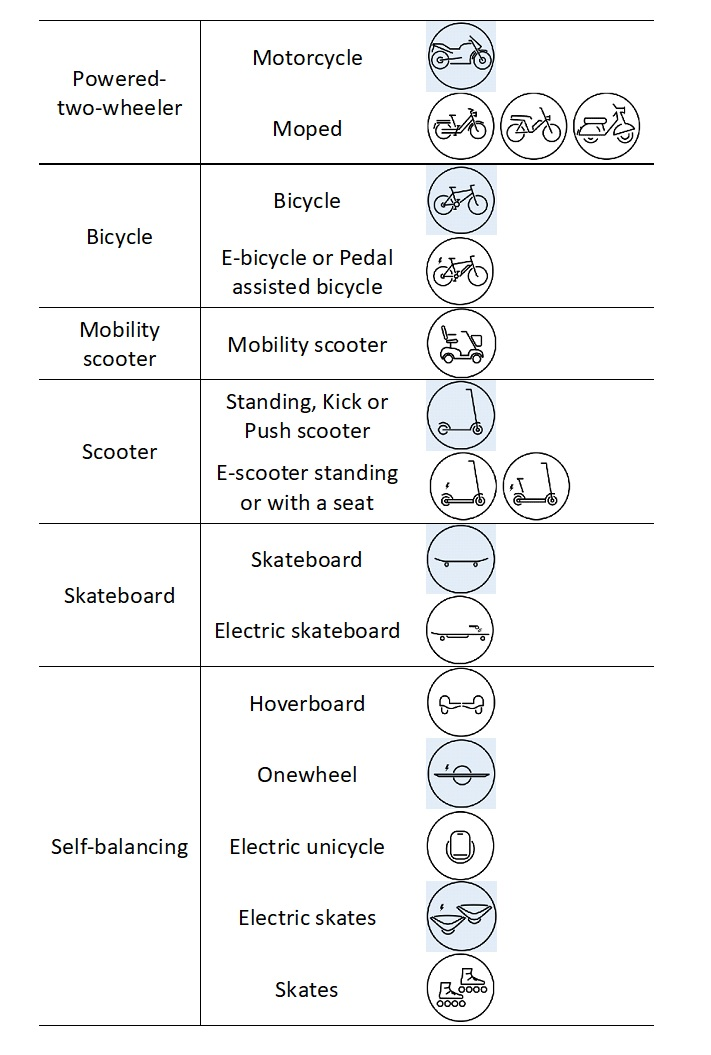
\includegraphics[width=0.5\linewidth]{image/micromobility} \caption{Mikromobilitaet (angepasst von OECD/ITF (2020)).}\label{fig:unnamed-chunk-23}
\end{figure}

Definitionen, Klassifizierungen und rechtliche Rahmenbedingungen für Mikromobilität sind weltweit unterschiedlich. Fahrräder sind in den meisten Ländern das kleinste Fahrzeug. Folglich sind eine Reihe von Kleinstfahrzeugen - wie E-Scooter, E-Skateboards und selbstbalancierende Fahrzeuge - von den Klassifizierungen ausgeschlossen. In einigen Fällen werden sie als Spielzeug eingestuft und sind daher nicht für den öffentlichen Straßenverkehr zugelassen. Als Übergangslösung hat Korea diese Geräte als Autos eingestuft. Die Behörden in Singapur haben beschlossen, eine neue Fahrzeugkategorie mit der Bezeichnung ``Personal Mobility Device'' (PMD) zu schaffen. Angesichts der offensichtlichen internationalen Bedeutung von Kleinstfahrzeugen und der Schwierigkeit, sie zu definieren und zu kategorisieren, könnte es sinnvoll sein, ein international anerkanntes Klassifizierungssystem für sie zu entwickeln (OECD/ITF, 2020).

In der \href{https://unece.org/resolutions}{Verordnung Nr. 168/2013 der Europäischen Union}, werden Fahrzeuge der Mikromobilität der Klasse L zugeordnet (UNECE, 2017). Fahrzeuge der Klasse L sind motorisierte zwei-, drei- und vierrädrige Fahrzeuge. Die Kategorie verwendet Leistung, Energiequelle, Geschwindigkeit, Länge, Breite und Höhe als Klassifizierungskriterien. Allerdings können nur ``Elektrofahrräder mit einer Höchstgeschwindigkeit von 25 km/h und einer Nutzleistung zwischen 250 Watt und 1 000 Watt'' und ``alle zweirädrigen Fahrzeuge mit einer bauartbedingten Höchstgeschwindigkeit von mehr als 25 km/h und bis zu 45 km/h und einer Nutzleistung von bis zu 4 000 Watt'' in die Klasse L1e der ``leichten zweirädrigen Kraftfahrzeuge'' eingestuft werden. Andere Kleinstfahrzeuge lassen sich in keine Kategorie einordnen. OECD/ITF (2020) schlägt vor, die Mikromobilität wie folgt zu klassifizieren:

\begin{figure}
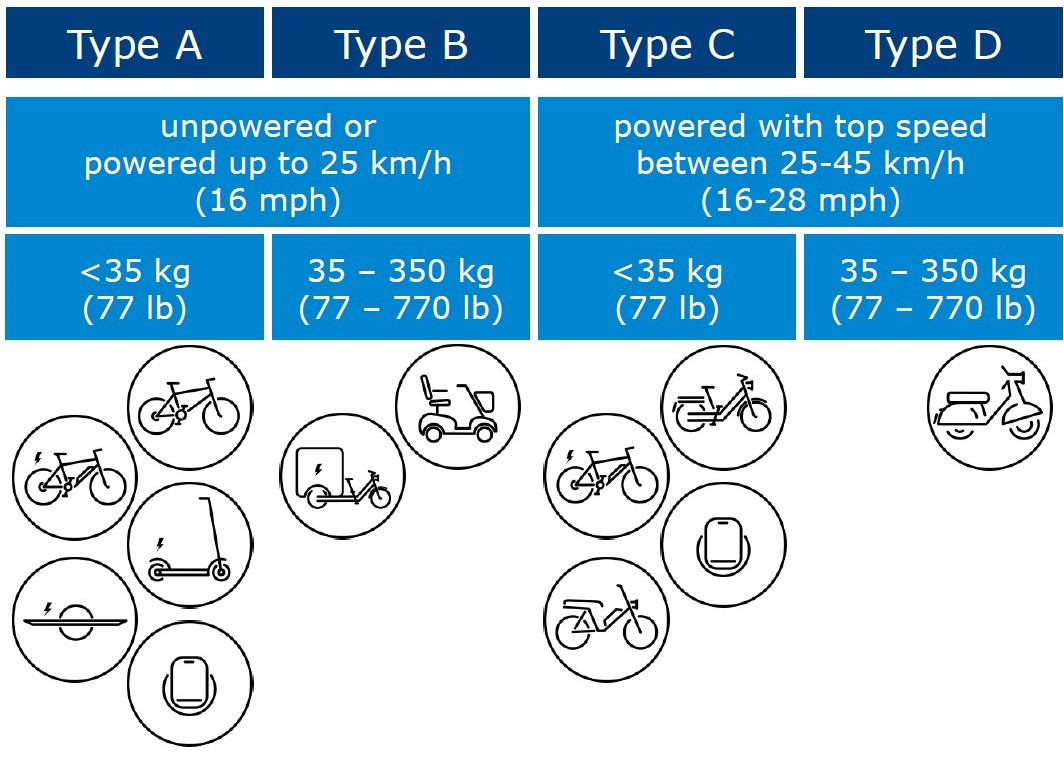
\includegraphics[width=0.5\linewidth]{image/micromobility_classes} \caption{Vorgeschlagene Klassifizierung von Geraeten der Mikromobilitaet (OECD/ITF (2020).}\label{fig:unnamed-chunk-24}
\end{figure}

Im Güterverkehr ist der \protect\hyperlink{intermodal_freight}{intermodale Güterverkehr} als Zubringer zu den Städten von entscheidender Bedeutung für die Reduzierung der Emissionen. Im Stadtzentrum (siehe \protect\hyperlink{urban_delivery}{Stadtlieferungen}) gibt es zwei Hauptbereiche, die praktische und relevante Lösungen für die Herausforderungen und die Effizienz des Güterverkehrs auf der letzten Meile bieten könnten: (1) Maßnahmen zur Steuerung der Frachtnachfrage (FDM) und (2) Verbesserung der Park- und Ladeinfrastruktur. Eine Maßnahme zur Nachfragesteuerung wäre die Förderung von Lieferungen außerhalb der Geschäftszeiten, um die Liefertätigkeit von Spediteuren und Verladern zu ändern. Außerdem könnten Empfängerpreise und Anreize eine wichtige Rolle bei der Reduzierung des Güterverkehrs spielen. (Holguín-Veras \& Sánchez-Díaz, 2016). In europäischen Städten (insbesondere in Frankreich) wird ein erheblicher Anteil an doppelt geparkten Lieferfahrzeugen (Lieferfahrzeuge, die auf der Straße parallel zu geparkten Autos abgestellt sind) beobachtet (Patier et al., 2014). In diesem Zusammenhang könnte die \protect\hyperlink{space_book}{intelligente Buchung von Lieferflächen} die Auswirkungen verringern. \protect\hyperlink{passenger_drones}{Passagierdrohnen} und \protect\hyperlink{electric_delivery_fleets}{Lieferflotten mit Elektrofahrzeugen} könnten ebenfalls einige der externen Effekte des Güterverkehrs in Städten reduzieren, aber sie könnten auch einige neue negative externe Effekte schaffen.

\hypertarget{wichtige-interessensgruppen-22}{%
\subsection*{Wichtige Interessensgruppen}\label{wichtige-interessensgruppen-22}}
\addcontentsline{toc}{subsection}{Wichtige Interessensgruppen}

\begin{itemize}
\tightlist
\item
  \textbf{Betroffene}: Alle Bürger:innen
\item
  \textbf{Verantwortliche}: Verkehrsdienstleister und Betreiber öffentlicher Verkehrsmittel, MaaS-Betreiber und -Integratoren, Stadtverwaltungen, lokale, regionale und nationale Behörden
\end{itemize}

\hypertarget{aktueller-stand-der-wissenschaft-und-forschung-22}{%
\subsection*{Aktueller Stand der Wissenschaft und Forschung}\label{aktueller-stand-der-wissenschaft-und-forschung-22}}
\addcontentsline{toc}{subsection}{Aktueller Stand der Wissenschaft und Forschung}

Die EUA (2019) kommt zu dem Schluss, dass eine bessere F/L/O-Meilen-Anbindung in Städten die Umwelt- und Gesundheitsergebnisse erheblich verbessern kann. Die Ausschöpfung dieses Potenzials erfordert jedoch ein tiefes Verständnis der verschiedenen Optionen, ihrer Stärken und Schwächen und ihrer Auswirkungen auf das Mobilitätssystem als Ganzes. Dies ist nicht immer einfach, da die Umwelt- und Gesundheitsauswirkungen von F/L/O-Mobilitätsoptionen davon abhängen, wie sie genutzt werden und was sie ersetzen. Dies unterstreicht die Tatsache, dass die zunehmende Verfügbarkeit von E-Scootern und digitalen Mitfahrplattformen das Mobilitätsverhalten in den Städten verändert, aber nicht immer die klimafreundlichere Wahl begünstigt. Ein einfaches Beispiel wäre eine kurze Fahrt mit einem E-Scooter. Wenn diese Fahrt eine Motorrad- oder Autofahrt ersetzt, sind die Auswirkungen auf Umwelt und Gesundheit positiv. Ersetzt sie eine Fahrt zu Fuß oder mit dem Fahrrad, verschlechtert sich die Situation. Mehr Transportmöglichkeiten können auch dazu führen, dass Menschen zusätzliche oder längere Fahrten unternehmen, was wiederum die Situation verschlechtern könnte. Darüber hinaus wird der öffentliche Verkehr ein wesentlicher Bestandteil jedes nachhaltigen städtischen Verkehrssystems bleiben. Gute F/L/O-Meilen-Optionen können den öffentlichen Verkehr attraktiver machen und seine Nutzung erhöhen, ihn aber nicht vollständig ersetzen (EUA, 2019). Laa \& Leth (2020) stellen außerdem fest, dass E-Scooter-Fahrten meist Fahrten ersetzen, die ansonsten mit einem nachhaltigeren Verkehrsmittel unternommen worden wären.

Im Hinblick auf die ökologische Nachhaltigkeit vergleichen Severengiz et al.~(2020) die „g CO\textsubscript{2} eq``/Personenkilometer (pkm) verschiedener Verkehrsträger (Abbildung 7.3). Moreau et al.~(2020) verglichen gemeinsam genutzte (shared) und private E-Scooter und berechneten 131g CO\textsubscript{2} eq/pkm für das geteilte Fahrzeug und 67g CO\textsubscript{2} eq/pkm für das private Fahrzeug.

\begin{figure}
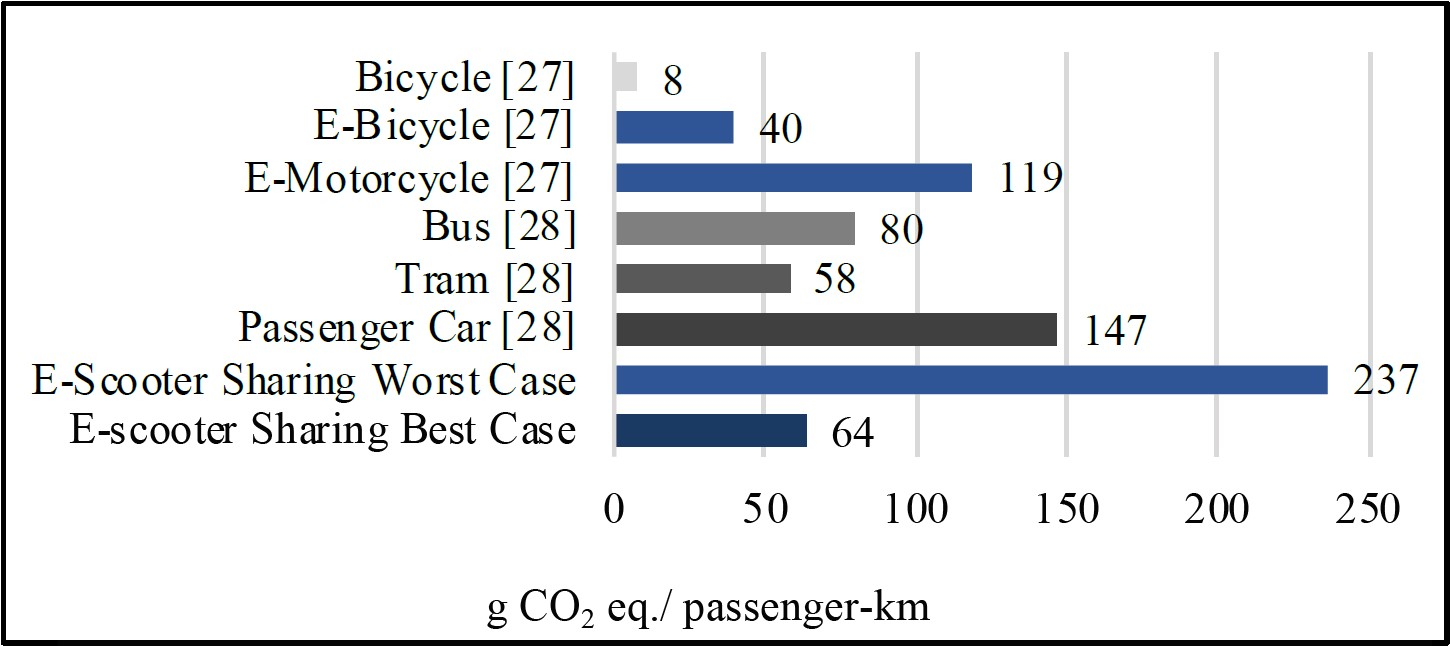
\includegraphics[width=0.5\linewidth]{image/flms_emissions} \caption{Vergleich der CO~2~-Aequivalent-Emissionen pro Personenkilometer der verschiedenen Verkehrstraeger (Severengiz et al., 2020)}\label{fig:unnamed-chunk-25}
\end{figure}

Erreichbarkeit ist ein Indikator für die Fähigkeit, häufig besuchte Orte effizient zu erreichen. Sie gewinnt zunehmend an Bedeutung als Ergänzung zu den traditionelleren mobilitätsbasierten Leistungskennzahlen in der Verkehrsplanung, wie z. B. durchschnittliche Verspätungen" und Dienstleistungsniveau". Die Bewertung der Leistung unter dem Aspekt der Erreichbarkeit bietet einen ausgewogenen, ganzheitlicheren Ansatz für die Verkehrsanalyse und -planung. Insbesondere werden alternative Strategien zur Verringerung von Staus und zur Milderung von Umweltproblemen in Betracht gezogen, wie z. B. die Förderung einer effizienten, ressourcenschonenden Flächennutzungspolitik. Erreichbarkeit ist ein Produkt aus Mobilität und Nähe, das entweder durch eine schnellere Verbindung zwischen Punkt A und Punkt B (Mobilität) oder durch eine größere Nähe zwischen den Punkten A und B (Nähe) oder durch eine Kombination dieser Faktoren verbessert wird. In diesem Sinne verleiht ein auf Erreichbarkeit basierender Ansatz Initiativen zur Flächennutzung und Instrumenten des Stadtmanagements Legitimität (Cervero, 2005).
Die Erreichbarkeit wird in der Literatur jedoch unterschiedlich definiert. Shin et al.~(2007) maßen die Erreichbarkeit anhand von Näherungsindizes (Entfernung und Gehzeit zur nächstgelegenen U-Bahn-Station). Martínez \& Viegas (2009) definierten die Erreichbarkeit anhand der Nähe zu öffentlichen Verkehrsknotenpunkten und dem Straßennetz. Bei gravitätsähnlichen Maßen wird die Erreichbarkeit einer Zone durch die Ziele bestimmt, die von dieser Zone aus erreicht werden können, negativ gewichtet durch die Reisezeit, Entfernung oder Kosten zwischen diesen beiden Zonen (Grengs et al., 2010). Beim isochronen Ansatz wird die Erreichbarkeit als die Anzahl der Ziele gemessen, die innerhalb einer bestimmten Reisezeit erreicht werden können (Cervero, 2005). Fan et al.~(2012) untersuchten die Auswirkungen der Einführung von Stadtbahnen auf die Verkehrsgerechtigkeit anhand der kumulierten 30-Minuten-Erreichbarkeit von Arbeitsplätzen mit öffentlichen Verkehrsmitteln. Die erste und letzte Meile ist eine wichtige Komponente einer Transitfahrt und bestimmt, ob der Transitdienst zugänglich ist oder nicht. Radfahren (oder andere FLM-Optionen) verringern die Ungleichheit im Verkehr, indem sie den Einzugsbereich des öffentlichen Verkehrs vergrößern, so dass die Menschen mehr Arbeitsplätze mit öffentlichen Verkehrsmitteln erreichen können (Zuo et al., 2020).

Die EEA (2019) fasst die Erkenntnisse für einen systemischen Wandel durch die Nutzung von First/Last/Only-Mobilitätsoptionen als Vorschläge für Regierungen wie folgt zusammen:
- Verdeutlichung der Auswirkungen von Mobilitätsentscheidungen und Angebot von Alternativen
- Konfrontation der Verkehrsteilnehmer:innen mit den Kosten ihrer Mobilitätsentscheidungen (Internalisierung der externen Kosten jedes Verkehrsmittels)
- Ausreichende und bequeme Alternativen anbieten
- Förderung des aktiven Verkehrs für die F/L/O - Mile
- Technologie mit den Zielen der nachhaltigen Mobilität in Einklang bringen

Bruzzone et al.~(2021) und Nocera et al.~(2020) untersuchen die Kombination von Personen- und Güterverkehrsströmen mit Schwerpunkt auf der letzten Meile. Bei einem solchen Modell handelt es sich um ein integriertes System, bei dem sich Fahrgäste und Güter Fahrzeuge, Infrastruktur, städtischen Raum oder mehr als eines dieser Elemente gleichzeitig teilen. Fatnassi et al.~(2015) zeigen beispielsweise die potenziellen Nachhaltigkeitsgewinne, die sich aus der gemeinsamen Nutzung von Gütern und Fahrgästen in einem Netz ergeben, wobei der Schwerpunkt auf der Verbesserung der Servicezeiten und der Energieverschwendung liegt.

In Bezug auf die Sicherheit stellen \href{https://www.itf-oecd.org/safe-micromobility}{OECD/ITF} 2020 fest, dass eine Fahrt mit dem Auto oder Motorrad in einem dichten städtischen Gebiet viel wahrscheinlicher zu tödlichen Unfällen von Verkehrsteilnehmer:innen führt als eine Fahrt mit einem Kleinstfahrzeug vom Typ A. Eine Verlagerung des Verkehrs von Kraftfahrzeugen auf Kleinstfahrzeuge des Typs A kann daher eine Stadt sicherer machen. Eine Verlagerung von Fußgänger:innen auf Kleinstfahrzeuge des Typs A hätte den gegenteiligen Effekt. Die Sicherheit von E-Scootern wird sich in den nächsten Jahren wahrscheinlich verbessern, wenn Nutzer:innen lernen, sich im Stadtverkehr zurechtzufinden, und sich Autofahrer:innen und Fußgänger:innen an die neuen Mobilitätsformen gewöhnen. Die Sicherheit wird sich auch verbessern, wenn die Regierungen eine sichere Fahrradinfrastruktur und gezielte Sicherheitsvorschriften für Kleinstfahrzeuge und Shared-Mobility-Dienste einführen. Aufgrund des rasanten Innovationstempos bei der Entwicklung von Kleinstfahrzeugen gibt es erhebliche regulatorische Herausforderungen. Sie schlagen folgende Maßnahmen vor, um die Sicherheit der Mikromobilität zu verbessern:

\begin{itemize}
\tightlist
\item
  Bereitstellung von geschütztem Raum für Mikromobilität und Sicherheit für Fußgänger:innen (Wenn sich Fußgänger:innen auf Gehwegen nicht sicher fühlen, wird die Zahl der Fußgänger:innen zurückgehen).
\item
  Niedrige Geschwindigkeiten von E-Scootern und E-Bikes sollten wie Fahrräder geregelt werden, höhere Geschwindigkeiten von Mikromobilen wie Mopeds
\item
  Sammlung von Daten über Fahrten mit Kleinstfahrzeugen und Unfälle (um die Sicherheit der Straßennetze proaktiv zu verwalten)
\item
  Einbindung der Mikromobilität in die Verkehrserziehung
\item
  Bekämpfung von Trunkenheit am Steuer und Geschwindigkeitsüberschreitungen bei allen Fahrzeugtypen
\item
  Beseitigung der Anreize für Fahrer:innen mikromobiler Fahrzeuge, zu schnell zu fahren (die minutengenaue Anmietung kann ein Anreiz sein, zu schnell zu fahren oder Verkehrsregeln zu ignorieren. Zu den Alternativen gehören eine feste Fahrgebühr, eine entfernungsabhängige Gebühr oder ein Mitgliedsbeitrag).
\item
  Verbesserung des Designs von Kleinstfahrzeugen (Hersteller von Kleinstfahrzeugen sollten versuchen, die Stabilität und Straßenhaftung zu verbessern. Lösungen könnten in Luftreifen, größeren Rädern und der Rahmengeometrie gefunden werden, aber auch in Bereichen, die noch erforscht werden müssen).
\item
  Verringerung der allgemeinen Risiken im Zusammenhang mit der gemeinsamen Nutzung von Mikromobilität (Minimierung der Fahrzeugkilometer, die von Begleitfahrzeugen für die Beförderung oder das Aufladen von Mikromobilitätsgeräten zurückgelegt werden, Verwendung von herausnehmbaren Batterien oder Batterien mit höherer Kapazität und Steckdosen, Bereitstellung von Flächen für das Parken von Mikrofahrzeugen auf der Straße).
\end{itemize}

\hypertarget{aktueller-stand-der-praktischen-umsetzung-22}{%
\subsection*{Aktueller Stand der praktischen Umsetzung}\label{aktueller-stand-der-praktischen-umsetzung-22}}
\addcontentsline{toc}{subsection}{Aktueller Stand der praktischen Umsetzung}

Eine neue Koalition, Micromobility for Europe (MMfE), hat sich 2021 in Europa zusammengeschlossen. Acht E-Scooter-Betreiber (Bird, Bolt, Dott, FreeNow, Lime, TIER, Voi und Wind) wollen durch diese Koalition zur Entwicklung eines kohärenten politischen Rahmens in Europa beitragen (Intelligent Transport, 2021).

Research and Markets (2021) nennt Bike-Sharing, Kick-Scooter-Sharing und Scooter-Sharing als die dominierenden Sharing-Modi für Mikromobilität. Bis 2020 wird der weltweite Fuhrpark auf rund 20,5 Millionen Fahrzeuge geschätzt. Der Anteil des Bike-Sharings an der weltweiten Flottengröße des Mikromobilitätsmarktes wird derzeit auf fast 98 \% geschätzt. Als wichtigster Faktor wird die Weiterentwicklung der Technologien genannt. Als Innovationen werden Infrastrukturlösungen (z. B. intelligente Andockstationen, solarbetriebene Ladestationen und Mobilitätshubs), Hardwarelösungen (z. B. intelligente Schlösser und Sensoren) und High-End-Softwarelösungen (z. B. Kartierung und Navigation, Flottensicherheit, Echtzeit-Flottendaten und -Analysen sowie intelligentes Flottenmanagement) genannt, die von KI-Maschinen und IoT-Sensoren angetrieben werden. Es wird auch erwähnt, dass sich die Geschäftsmodelle der Mikromobilität weiterentwickeln. So gibt es beispielsweise bereits öffentlich-private Partnerschaften, private Bike-Sharing-Systeme und gemeinnützige Programme. Es wird erwartet, dass Mikromobilitätssysteme weiterhin in den kommunalen Verkehr eingebettet werden und ein integraler Bestandteil des entstehenden Mobility-as-a-Service-Ökosystems (MaaS) werden.

Im Jahr 2018, dem ersten vollen Jahr nach der Einführung des E-Scooter-Sharings, haben die Amerikaner bereits 38,5 Millionen Fahrten mit gemeinsam genutzten E-Scootern unternommen (im Vergleich zum stationsbasierten Bike-Sharing mit 36,5 Millionen Fahrten, das seit fast zehn Jahren auf dem Markt ist). Die bestehende Nachfrage nach anderer Mikromobilität ist jedoch nicht zurückgegangen. Das zeigt, dass es sinnvoll ist, verschiedene Modelle/Fahrzeuge zu unterstützen. In Anbetracht der hohen Nachfrage und der raschen Akzeptanz von Mikromobilitätsoptionen liegt das erwartete weltweite Marktpotenzial bis 2030 bei über 500 Milliarden Dollar (Eliasen, 2021). Im Vergleich dazu wird der Mikromobilitätsmarkt in Europa auf über 100 Milliarden Euro im Jahr 2030 geschätzt (Twisse, 2020). Die meisten Neugründungen von Mikromobilitätsplattformen (hauptsächlich E-Scooter) waren jedoch anfangs unrentabel, da die Betriebskosten für den Betrieb von E-Scootern (Aufladen, Reparatur/Wartung, Versicherungs- und Zahlungsgebühren) so hoch waren, dass die Amortisationszeit für den anfänglichen Rollerkauf kürzer war als die Lebensdauer des Rollers, was zu einer negativen Investitionsrendite pro Roller führte. Laut Travis VanderZanden, CEO von Bird, hat sich die Rentabilität der Einheiten in den letzten Jahren aufgrund der verbesserten Haltbarkeit der Roller und der Preiserhöhungen für die Kund:innen deutlich verbessert (Eliasen, 2021).

Haas (2018) nennt vier Herausforderungen, die es für die Attraktivität der FLM zu bewältigen gilt:

\textbf{Herausforderung 1: Erreichbarkeit}
Es kommt häufig vor, dass in der Nähe kein Sharing-Transport angeboten werden kann. \emph{``Im Durchschnitt sind unsere Kund:innen bereit, 300 Meter zu Fuß zu einem Auto zu gehen''}, sagt Olivier Reppert (Chef des Carsharing-Marktführers Car2go). \emph{``Wenn das mehrmals nicht klappt, springen sie ab.''} Das Unternehmen arbeitet deshalb intensiv daran, die Fahrzeuge so nah wie möglich an die Kund:innen zu bringen. \emph{``Wir wissen sehr genau, wo welches Auto zu welcher Zeit stehen sollte''}, sagt Reppert. Das lässt sich durch anonyme Datenerfassung genau bestimmen. Aber: \emph{``Heute sind wir noch nicht in der Lage, immer genau diese Punkte anzusteuern.'' } Große Hoffnungen setzt Reppert auf den künftigen Einsatz von automatisierten Fahrzeugen, die sich selbst zu Carsharing-Hotspots bewegen: \emph{``Dann bräuchten wir nur noch 50 Prozent der heutigen Flotte, um die gleiche Nachfrage zu bedienen''}, sagt er..

\textbf{Herausforderung zwei: Die Kombination}
Um die perfekte Kombination der verschiedenen Angebote zu ermöglichen, wird eine App benötigt, die alle Optionen umfasst und aufeinander abstimmt. Bislang gibt es nur wenige solcher Apps mit möglichst vielen Verkehrsmitteln in den Städten. Das könnte sich verbessern, wenn die Städte, die den besten Überblick über die verfügbaren Verkehrsmittel in ihrem Gebiet haben sollten, selbst die Führung übernehmen.

\textbf{Herausforderung drei: Die rechtliche Situation}
\emph{``Wenn sich verschiedene Kleinfahrzeuge einfach die Geh- und Radwege oder die Straßen teilen, führt das zu mehr Unfällen''}, sagt Markus Friedrich (Professor für Verkehrsplanung und Verkehrsleittechnik an der Universität Stuttgart). Der Platz reicht aber nicht aus, um für jeden Typ eine eigene Spur anzubieten. Die Lösung sieht er daher in einer Änderung der aktuellen Geschwindigkeitsbegrenzung in der Straßenverkehrsordnung: \emph{``Mit einer Regelgeschwindigkeit von 30 km/h können sich die Fahrzeuge den Straßenraum besser teilen''}, sagt der Professor. \emph{"Und sobald viele Fahrzeuge über Elektroantriebe verfügen, ist in den heutigen Tempo-30-Zonen ein Limit von 20km/h denkbar. }" Auf innerstädtischen Hauptverkehrsstraßen könnten noch höhere Geschwindigkeiten erlaubt sein.

\textbf{Herausforderung vier: Der Ausbau des öffentlichen Verkehrs}
Die zahlreichen zusätzlichen Dienste könnten Bus und Bahn nicht nur ergänzen, sondern ersetzen. Die Nachfrage könnte erheblich steigen, wenn sich die Vorteile der gewonnenen Effizienz entfalten - von höherer Verfügbarkeit bis zu günstigeren Preisen. Deshalb muss der öffentliche Verkehr schneller werden, damit er einen Fahrzeitvorteil bietet. Nötig sind laut Friedrich Schnellbusse und Schnellzüge, die eigene Routen bekommen und nicht mehr so oft halten wie bisher. Viele Städte bräuchten eine wesentlich dichtere Taktung oder zusätzliche Expresszüge.

\hypertarget{relevante-initiativen-in-uxf6sterreich-22}{%
\subsection*{Relevante Initiativen in Österreich}\label{relevante-initiativen-in-uxf6sterreich-22}}
\addcontentsline{toc}{subsection}{Relevante Initiativen in Österreich}

\textbf{Passenger FLM}

\begin{itemize}
\tightlist
\item
  E-scooters

  \begin{itemize}
  \tightlist
  \item
    \href{https://autorevue.at/ratgeber/e-scooter-wien-vergleich}{Autorevue.at}
  \item
    \href{https://www.stadt-wien.at/wien/news/e-scooter-sharing-system-in-wien.html}{Stadt-wien.at}
  \item
    \href{https://www.wien.gv.at/verkehr/scooter-roller/index.html}{Wien.gv.at}
  \item
    \href{https://www.oeamtc.at/thema/fahrrad/e-kleintretroller-e-scooter-in-oesterreich-31721872}{Öamtc.at}
  \item
    \href{https://www.oesterreich.gv.at/themen/freizeit_und_strassenverkehr/Elektro-Scooter,-Quads-und-Co/Seite.610110.html}{Österreich.gv.at}
  \end{itemize}
\item
  Bicycle and E-Bicycle hire

  \begin{itemize}
  \tightlist
  \item
    \href{https://firmenradl.at/cms/}{Firmenradl.at}
  \item
    \href{https://www.citybikewien.at/de}{Citybikewien}
  \item
    \href{http://www.citybikesalzburg.at/}{Citybikesalzburg}
  \item
    \href{https://www.nextbike.at/de/niederoesterreich/}{Nextbike}
  \item
    \href{https://www.tips.at/nachrichten/linz/land-leute/523512-linzer-radverleih-startet-im-fruehjahr-an-40-standorten}{Tpis.at}
  \end{itemize}
\item
  Car sharing

  \begin{itemize}
  \tightlist
  \item
    \href{https://www.vcoe.at/presse/presseaussendungen/detail/carsharing-haushalte-potential-2018}{VCÖ}
  \item
    \href{https://www.carsharing-wien.com/anbieter/oebb-rail-and-drive}{ÖBB}
  \end{itemize}
\item
  Ride-hailing \& Ride-sharing

  \begin{itemize}
  \tightlist
  \item
    \href{https://www.ots.at/presseaussendung/OTS_20210113_OTS0026/free-now-will-als-erste-mobilitaetsplattform-in-europa-bis-2030-null-emissionen-erreichen}{Ots.at}
  \item
    \href{https://www.umweltberatung.at/carsharing-mitfahrboersen}{Umweltberatung.at}
  \item
    \href{https://greendrive.at/premium/\#benefits}{Greendrive.at}
  \item
    \href{https://www.carployee.com/\#start-section}{Carployee.com}
  \item
    \href{https://ummadum.com/}{Ummadum.com}
  \end{itemize}
\item
  Mobility-as-a-Service

  \begin{itemize}
  \tightlist
  \item
    \href{https://www.austriatech.at/assets/Uploads/Publikationen/PDF-Dateien/29fc02ada2/MaaS-miA_english_102019_web.pdf}{AustriaTech.at}
  \item
    \href{https://maas-ready.at}{maas-ready.at}
  \item
    \href{https://www.ultimob.at}{ultimob.at}
  \item
    \href{https://www.tim-oesterreich.at/graz/}{tim-oesterreich.at}
  \item
    \href{https://wegfinder.at/}{wegfinder.at}
  \item
    \href{https://www.wienerlinien.at/eportal3/ep/channelView.do/pageTypeId/66526/channelId/-3600060}{wienerlinien.at}
  \item
    \href{https://anachb.vor.at/}{anachb.vor.at}
  \end{itemize}
\item
  Passenger drones

  \begin{itemize}
  \tightlist
  \item
    \href{https://brutkasten.com/autonome-lufttaxis-linz-ag-facc-ehang/}{Derbrutkasten.com}
  \item
    \href{https://www.derstandard.at/consent/tcf/story/2000103120464/erste-teststrecke-fuer-e-lufttaxis-2020-in-linz}{Derstandard.at-1}
  \item
    \href{https://www.derstandard.at/consent/tcf/story/2000122402408/flugtaxis-wann-kommt-der-tesla-der-luefte}{Derstandard.at-2}
  \end{itemize}
\item
  Demand responsive transit

  \begin{itemize}
  \tightlist
  \item
    \href{https://www.bedarfsverkehr.at/content/Literatur}{Bedarfsverkehr.at}
  \item
    \href{https://repositum.tuwien.at/handle/20.500.12708/1312}{Repositum.tuwien.at}
  \item
    \href{https://projekte.ffg.at/projekt/2929323}{Projekte.ffg.at}
  \end{itemize}
\item
  Mobility hubs

  \begin{itemize}
  \tightlist
  \item
    \href{https://www.wienerlinien.at/web/wiener-linien/wienmobil-stationen}{Wienmobil-stationen}
  \item
    \href{https://www.tim-oesterreich.at/}{Tim-oesterreich}
  \item
    \href{https://www.wien.gv.at/stadtentwicklung/studien/pdf/b008521.pdf}{Wien.gv.at}
  \end{itemize}
\end{itemize}

\textbf{Freight FLM}

\begin{itemize}
\tightlist
\item
  Urban Deliveries

  \begin{itemize}
  \tightlist
  \item
    \href{https://www.logistik2030.at/?page_id=268}{Logistik2030.at-1}
  \item
    \href{https://infothek.bmk.gv.at/gruene-stadtlogistik-post-testet-city-hubs-in-wien/}{Infothek.bmk.gv.at}
  \item
    \href{https://www.logistik2030.at/?page_id=63}{Logistik2030.at-2}
  \item
    \href{https://www.remihub.at/}{Remihub.at}
  \item
    \href{https://logpoint.at/ueber-uns/gruene-logistikwelt-und-standorte/}{Logpoint.at}
  \item
    \href{https://www.wu.ac.at/scm/projekte/}{Wu.ac.at}
  \item
    \href{https://www.post.at/p/c/vorzimmer-zustellung}{Post.at}
  \end{itemize}
\item
  Smart delivery space booking

  \begin{itemize}
  \tightlist
  \item
    \href{https://www.ots.at/presseaussendung/OTS_20150123_OTS0044/simple-stressfreie-ladezonensuche-wk-wien-praesentiert-neue-app}{Ots.at}
  \item
    \href{https://www.wko.at/service/verkehr-betriebsstandort/Ladezonen-Nutzung.html}{WKO1}
  \item
    \href{https://www.wko.at/service/w/verkehr-betriebsstandort/ladezone-wien-app.html}{WKO2}
  \item
    \href{https://www2.ffg.at/verkehr/projekte.php?id=805\&lang=de\&browse=programm}{FFG}
  \end{itemize}
\item
  Delivery drones

  \begin{itemize}
  \tightlist
  \item
    \href{https://www.oeamtc.at/thema/drohnen/drohnen-info-app-26853120}{Öamtc.at}
  \end{itemize}
\item
  Freight hubs

  \begin{itemize}
  \tightlist
  \item
    \href{https://infrastruktur.oebb.at/en/partners/terminals/locations/terminal-wien-sued}{Infrastruktur.oebb.at}
  \item
    \href{https://dhl-freight-connections.com/de/unternehmen/dhl-eroffnet-hochmodernes-logistikdrehkreuz-am-flughafen-wien/}{DHL-freight-connections.com}
  \item
    \href{https://www.logistik2030.at/?page_id=63}{Logistik2030.at}
  \item
    \href{https://www.thinkportvienna.at/ueber-uns/projekte/}{Thinkportvienna.at}
  \item
    \href{https://www.hafen-wien.com/de/home}{Hafen-wien.com}
  \end{itemize}
\end{itemize}

\hypertarget{auswirkungen-in-bezug-auf-die-ziele-fuxfcr-nachhaltige-entwicklung-sdgs-22}{%
\subsection*{Auswirkungen in Bezug auf die Ziele für nachhaltige Entwicklung (SDGs)}\label{auswirkungen-in-bezug-auf-die-ziele-fuxfcr-nachhaltige-entwicklung-sdgs-22}}
\addcontentsline{toc}{subsection}{Auswirkungen in Bezug auf die Ziele für nachhaltige Entwicklung (SDGs)}

\begin{longtable}[]{@{}ccccc@{}}
\toprule
\begin{minipage}[b]{0.17\columnwidth}\centering
Ebene der Auswirkungen\strut
\end{minipage} & \begin{minipage}[b]{0.16\columnwidth}\centering
Indikator\strut
\end{minipage} & \begin{minipage}[b]{0.17\columnwidth}\centering
Richtung der Auswirkungen\strut
\end{minipage} & \begin{minipage}[b]{0.17\columnwidth}\centering
Beschreibung des Ziels \& SDG\strut
\end{minipage} & \begin{minipage}[b]{0.17\columnwidth}\centering
Beschreibung des Ziels \& SDG\strut
\end{minipage}\tabularnewline
\midrule
\endhead
\begin{minipage}[t]{0.17\columnwidth}\centering
Systemisch\strut
\end{minipage} & \begin{minipage}[t]{0.16\columnwidth}\centering
Verringerung der Ungleichheit bei den Verkehrsdiensten\strut
\end{minipage} & \begin{minipage}[t]{0.17\columnwidth}\centering
\textbf{+}\strut
\end{minipage} & \begin{minipage}[t]{0.17\columnwidth}\centering
Gleichheit (\emph{5,10})\strut
\end{minipage} & \begin{minipage}[t]{0.17\columnwidth}\centering
Zuo et al., 2020a\strut
\end{minipage}\tabularnewline
\begin{minipage}[t]{0.17\columnwidth}\centering
Systemisch\strut
\end{minipage} & \begin{minipage}[t]{0.16\columnwidth}\centering
Verringerung negativer externer Effekte, aber Substitution durch umweltfreundlichere Verkehrstraeger, z. B. zu Fuss\strut
\end{minipage} & \begin{minipage}[t]{0.17\columnwidth}\centering
\textbf{\textasciitilde{}}\strut
\end{minipage} & \begin{minipage}[t]{0.17\columnwidth}\centering
Oekologische Nachhaltigkeit (\emph{7,12,13,15})\strut
\end{minipage} & \begin{minipage}[t]{0.17\columnwidth}\centering
Twisse, 2020\strut
\end{minipage}\tabularnewline
\begin{minipage}[t]{0.17\columnwidth}\centering
Systemisch\strut
\end{minipage} & \begin{minipage}[t]{0.16\columnwidth}\centering
Gewinne aus dem Wachstum des Mikromobilitaetssektors (F/L/O-Optionen)\strut
\end{minipage} & \begin{minipage}[t]{0.17\columnwidth}\centering
\textbf{+}\strut
\end{minipage} & \begin{minipage}[t]{0.17\columnwidth}\centering
Nachhaltige wirtschaftliche Entwicklung (\emph{8,11})\strut
\end{minipage} & \begin{minipage}[t]{0.17\columnwidth}\centering
Goessling, 2020\strut
\end{minipage}\tabularnewline
\begin{minipage}[t]{0.17\columnwidth}\centering
Systemisch\strut
\end{minipage} & \begin{minipage}[t]{0.16\columnwidth}\centering
Verbesserung der Technologie von Mikromobilitaetsgeraeten\strut
\end{minipage} & \begin{minipage}[t]{0.17\columnwidth}\centering
\textbf{+}\strut
\end{minipage} & \begin{minipage}[t]{0.17\columnwidth}\centering
Innovation und Infrastruktur (\emph{9})\strut
\end{minipage} & \begin{minipage}[t]{0.17\columnwidth}\centering
Eliasen, 2021\strut
\end{minipage}\tabularnewline
\bottomrule
\end{longtable}

\hypertarget{technologie--und-gesellschaftlicher-bereitschaftsgrad-19}{%
\subsection*{Technologie- und gesellschaftlicher Bereitschaftsgrad}\label{technologie--und-gesellschaftlicher-bereitschaftsgrad-19}}
\addcontentsline{toc}{subsection}{Technologie- und gesellschaftlicher Bereitschaftsgrad}

\begin{longtable}[]{@{}cc@{}}
\toprule
Stand der Technologiebereitschaft & Gesellschaftlicher Bereitschaftsgrad\tabularnewline
\midrule
\endhead
7-9 & 6-7\tabularnewline
\bottomrule
\end{longtable}

\hypertarget{weitere-links-18}{%
\subsection*{Weitere links}\label{weitere-links-18}}
\addcontentsline{toc}{subsection}{Weitere links}

\begin{itemize}
\tightlist
\item
  \href{https://unece.org/resolutions}{UNECE.org}
\item
  \href{https://www.eltis.org/resources/case-studies/rise-micromobility}{ELTIS.org}
\end{itemize}

\hypertarget{referenzen-22}{%
\subsection*{Referenzen}\label{referenzen-22}}
\addcontentsline{toc}{subsection}{Referenzen}

\begin{itemize}
\tightlist
\item
  Arvidsson, N., Givoni, M., \& Woxenius, J. (2016). Exploring last mile synergies in passenger and freight transport. Built Environment, 42(4), 523â€``538. \url{https://doi.org/10.2148/benv.42.4.523}
\item
  Bruzzone, F., Cavallaro, F., \& Nocera, S. (2021). The integration of passenger and freight transport for first-last mile operations. Transport Policy, 100, 31-48. \url{https://doi.org/10.1016/j.tranpol.2020.10.009}
\item
  Cervero, R. (2005). Accessible Cities and Regions: A Framework for Sustainable Transport and Urbanism in the 21st Century. \url{https://doi.org/10.11436/mssj.15.250}
\item
  City database \textbar{} Eltis. (2021, July 19). \url{https://www.eltis.org/mobility-plans/city-database}
\item
  EEA, E. E. A. (2019). The first and last mile - the key to sustainable urban transport (Issue 18).
\item
  Eliasen, J. (2021, January 15). The Future of Micromobility. How VCs and E-Scooters kicked off the… \textbar{} by Jason Eliasen \textbar{} The Startup \textbar{} Medium. \url{https://medium.com/swlh/the-future-of-micromobility-2d4d96d4e2dd}
\item
  Fan, Y., Guthrie, A., \& Levinson, D. (2012). Impact of light-rail implementation on labor market accessibility. Journal of Transport and Land Use, 5(3), 28-39.
\item
  Fatnassi, E., Chaouachi, J., \& Klibi, W. (2015). Planning and operating a shared goods and passengers on-demand rapid transit system for sustainable city-logistics. Transportation Research Part B: Methodological, 81, 440-460. \url{https://doi.org/10.1016/j.trb.2015.07.016}
\item
  Furth, P. G., Mekuria, M. C., \& Nixon, H. (2016). Network Connectivity for Low-Stress Bicycling. Transportation Research Record, 2587(1), 41-49. \url{https://doi.org/10.3141/2587-06}
\item
  Gössling, S. (2020). Integrating e-scooters in urban transportation: Problems, policies, and the prospect of system change. Transportation Research Part D: Transport and Environment, 79(January), 102230. \url{https://doi.org/10.1016/j.trd.2020.102230}
\item
  Grengs, J., Levine, J., Shen, Q., \& Shen, Q. (2010). Intermetropolitan Comparison of Transportation Accessibility: Sorting Out Mobility and Proximity in San Francisco and Washington, D.C. Journal of Planning Education and Research, 29(4), 427-443. \url{https://doi.org/10.1177/0739456X10363278}
\item
  Haas, C. (2018, November 13). Nahverkehr: So lässt sich die letzte Meile nach Hause bequem zurücklegen - WELT. \url{https://www.welt.de/wirtschaft/article183688842/Nahverkehr-So-laesst-sich-die-letzte-Meile-nach-Hause-bequem-zuruecklegen.html}
\item
  Holguín-Veras, J., \& Sánchez-Díaz, I. (2016). Freight Demand Management and the Potential of Receiver-Led Consolidation programs. Transportation Research Part A: Policy and Practice, 84, 109-130. \url{https://doi.org/10.1016/j.tra.2015.06.013}
\item
  Intelligent Transport. (2021, February 2). Big names across micromobility sector form European coalition. \url{https://www.intelligenttransport.com/transport-news/116405/micromobility-for-europe/}
\item
  Laa, B., \& Leth, U. (2020). Survey of E-scooter users in Vienna: Who they are and how they ride. Journal of Transport Geography, 89(October), 102874. \url{https://doi.org/10.1016/j.jtrangeo.2020.102874}
\item
  Martínez, L. M., \& Viegas, J. M. (2009). Effects of Transportation Accessibility on Residential Property Values: Hedonic Price Model in the Lisbon, Portugal, Metropolitan Area. Transportation Research Record, 2115(1), 127-137. \url{https://doi.org/10.3141/2115-16}
\item
  Moreau, H., de Meux, L. J., Zeller, V., D’Ans, P., Ruwet, C., \& Achten, W. M. J. (2020). Dockless e-scooter: A green solution for mobility? Comparative case study between dockless e-scooters, displaced transport, and personal e-scooters. Sustainability (Switzerland), 12(5). \url{https://doi.org/10.3390/su12051803}
\item
  Nocera, S., Pungillo, G., \& Bruzzone, F. (2020). How to evaluate and plan the freight-passengers first-last mile. Transport Policy. \url{https://doi.org/10.1016/j.tranpol.2020.01.007}
\item
  OECD/ITF. (2020). Safe Micromobility. 98.
\item
  Oeschger, G., Carroll, P., \& Caulfield, B. (2020). Micromobility and public transport integration: The current state of knowledge. Transportation Research Part D: Transport and Environment, 89, 102628. \url{https://doi.org/10.1016/j.trd.2020.102628}
\item
  Patier, D., David, B., Chalon, R., \& Deslandres, V. (2014). A New Concept for Urban Logistics Delivery Area Booking. Procedia - Social and Behavioral Sciences, 125, 99-110. \url{https://doi.org/10.1016/j.sbspro.2014.01.1459}
\item
  Research and Markets. (2021, June 15). Global Micromobility (Bikes, Scooters, Kick-scooters) Markets Report 2021-2025 - Future Growth Potential Enhanced by Opportunities Due to Government Push, Regulatory Reforms and Advancement in Technologies. \url{https://www.prnewswire.com/news-releases/global-micromobility-bikes-scooters-kick-scooters-markets-report-2021-2025---future-growth-potential-enhanced-by-opportunities-due-to-government-push-regulatory-reforms-and-advancement-in-technologies-301312406.html}
\item
  Severengiz, S., Finke, S., Schelte, N., \& Wendt, N. (2020). Life Cycle Assessment on the Mobility Service E-Scooter Sharing. 2020 IEEE European Technology and Engineering Management Summit, E-TEMS 2020, September. \url{https://doi.org/10.1109/E-TEMS46250.2020.9111817}
\item
  Shin, K., Washington, S., \& Choi, K. (2007). Effects of Transportation Accessibility on Residential Property Values: Application of Spatial Hedonic Price Model in Seoul, South Korea, Metropolitan Area. Transportation Research Record, 1994(1), 66-73. \url{https://doi.org/10.3141/1994-09}
\item
  Twisse, F. (2020, August 12). The rise of micromobility \textbar{} Eltis. \url{https://www.eltis.org/resources/case-studies/rise-micromobility}
\item
  UNECE. (2017). ECE R78 - Consolidated Resolution on the Construction of Vehicles. United Nations Economic and Social Council, July. Available at: \url{https://unece.org/resolutions} (Accessed: 22/07/2021)
\item
  Winters, M., Davidson, G., Kao, D., \& Teschke, K. (2011). Motivators and deterrents of bicycling: Comparing influences on decisions to ride. Transportation, 38(1), 153-168. \url{https://doi.org/10.1007/s11116-010-9284-y}
\item
  Zuo, T., Wei, H., Chen, N., \& Zhang, C. (2020a). First-and-last mile solution via bicycling to improving transit accessibility and advancing transportation equity. Cities, 99, 102614. \url{https://doi.org/10.1016/j.cities.2020.102614}
\item
  Zuo, T., Wei, H., \& Rohne, A. (2018). Determining transit service coverage by non-motorized accessibility to transit: Case study of applying GPS data in Cincinnati metropolitan area. Journal of Transport Geography, 67, 1-11. \url{https://doi.org/10.1016/j.jtrangeo.2018.01.002}
\end{itemize}

\hypertarget{dist_time_fares}{%
\section{Transit fares}\label{dist_time_fares}}

\hypertarget{definition-23}{%
\subsection*{Definition}\label{definition-23}}
\addcontentsline{toc}{subsection}{Definition}

Fahrpreise sind ein grundlegendes Element des Verkehrsbetriebs, sie haben einen wichtigen Einfluss auf die Fahrgastdynamik und die finanzielle Vitalität von Verkehrsbetrieben (El-Geneidy et al., 2016; Zhao \& Zhang, 2019). Die Art und Weise, wie Fahrpreise festgelegt und anschließend angepasst werden, ist von Natur aus komplex. Einerseits wird versucht, Gerechtigkeit für die Bevölkerung zu gewährleisten, andererseits sollen ausreichende Einnahmen für das Verkehrsunternehmen generiert werden (Brown, 2018; Yoh et al., 2016). In der aktuellen Verkehrsforschung wird argumentiert, dass Fahrpreise und insbesondere Tarifstrukturen (wie zonen- oder entfernungsabhängige Tarife) negative Auswirkungen auf die Gerechtigkeit haben, obwohl es auch Belege dafür gibt, dass es davon abhängt, wo man wohnt und wie dies den Grad der Zugänglichkeit beeinflusst (Martens, 2012).

Es gibt keine allgemeingültige Definition von Gerechtigkeit im Zusammenhang mit dem öffentlichen Verkehr, aber verschiedene Möglichkeiten, Gerechtigkeit aus unterschiedlichen Perspektiven zu messen, wie z. B. Reiseentfernung, Zeit, Komfort und monetäre Kosten. Eine notwendige Voraussetzung für die wissenschaftliche Messung der Gerechtigkeit im öffentlichen Verkehr ist die Konzentration auf eine bestimmte Dimension, wie z. B. die monetären Kosten (Fahrpreise) (Wang et al., 2021).

In der Literatur zur Verteilungsgerechtigkeit werden drei Dimensionen für die Bewertung der Fairness unterschieden (Rubensson et al., 2020):
- Eine normative Dimension - die Grundlagen des Fairnessprinzips: z. B. sollten alle Ergebnisse so ähnlich wie möglich sein, oder sollten alle Personen so ähnliche Chancen wie möglich haben, oder sollte man darauf vertrauen, dass gut regulierte Märkte das gerechteste Ergebnis hervorbringen?
- Die Autor:innen wählen aus, was sie messen wollen - Gerechtigkeit der Inputs (Fahrpreise, Steuern), der Outputs (Zugänglichkeit, geografische Abdeckung) oder Verbrauch (durchgeführte Fahrten) des öffentlichen Verkehrs.
- Verteilungsunterschiede - Bewertung der horizontalen Gerechtigkeit (Gerechtigkeit zwischen Mitgliedern derselben Gruppe, z. B. allen Nutzer:innen des öffentlichen Verkehrs oder allen Bürger:innen) oder der vertikalen Gerechtigkeit (Gerechtigkeit zwischen Mitgliedern verschiedener Gruppen, z. B. verschiedener Einkommens-, Alters- oder Berufsgruppen).

Ein Tarifsystem umfasst in der Regel vier grundlegende Komponenten (Streeting \& Charles, 2006):
- Tarifmedien - Papiertickets oder Chipkarten
- Tarifprodukt - Palette der verfügbaren Fahrscheintypen, z. B. frequenzabhängige Ermäßigungen und Ermäßigungen außerhalb der Hauptverkehrszeiten, Begrenzung des Fahrpreises auf einen festen Höchstbetrag an Wochenenden (Chalabianlou et al., 2015; Guzman et al., 2014)
- Tarifstruktur
Fahrpreisniveau - Fahrpreise können pauschal oder differenziert festgelegt werden. Eine Differenzierung wird in der Regel vorgeschlagen, um ein Tarifsystem zu erreichen, das die Nachfrage nach Fahrten mit hohen Produktionskosten senkt und die Nachfrage nach Fahrten mit niedrigen Produktionskosten erhöht, wodurch einerseits die Einnahmen erhöht und andererseits die Preise für einige Nutzer:innen gesenkt werden (Rubensson et al., 2020).

Die verschiedenen Tarifstrukturen sind (Wang et al., 2021):

\begin{itemize}
\tightlist
\item
  \textbf{Pauschaltarife } (ein einziger Tarif für das gesamte Tarifsystem)
\item
  \textbf{Entfernungsabhängige Tarife} (Tarife werden nach Entfernung berechnet)
  Bei einem entfernungsabhängigen System werden für Fahrgäste, die längere Strecken zurücklegen, höhere Tarife berechnet. Die Tarife werden in der Regel für jede einzelne Strecke auf der Grundlage der Entfernung zwischen Ausgangs- und Zielort (OD - origin and destination) berechnet. Entfernungsabhängige Tarife sind in der Regel kompliziert zu entwickeln und durchzusetzen, da sie eine Karte erfordern, die durchgestrichen, angezapft oder gelocht werden muss, oder sie erfordern eine Schranke, die eine zusätzliche Zahlung erzwingt. Entfernungsabhängige Preise werden nur selten auf Nicht-Express-Strecken und im Schienenverkehr verwendet, sondern eher auf Expressstrecken und Systemen, die von einem zentralen Bereich ausgehen (McKone, 2010).
\item
  \textbf{Zeitabhängige Tarife} (nach Fahrzeit berechnete Tarife)
  Das zeitbasierte System ermöglicht es den Fahrgästen, öffentliche Verkehrsmittel zu nutzen und innerhalb eines bestimmten Zeitraums kostenlos umzusteigen. Die Gültigkeitsdauer kann so kurz wie 20 Minuten sein (Krakow.pl, 2021) oder eine unbegrenzte Wochen-, Monats- oder Jahreskarte (Wiener Linien, 2021). Wichtig ist, dass dieses Preissystem eine Art von Karte (Papier-, Magnet- oder Chipkarte) erfordert, um den Transfer auszustellen. Es wird häufig für innerstädtische öffentliche Verkehrslösungen verwendet
\item
  \textbf{Zonenbasierte Tarife} (Tarife, die nach Reisezone berechnet werden)
  Die Fahrpreise werden in der Regel auf der Grundlage von Zonen berechnet, die in bestimmten Regionen der Stadt steigende Fahrpreise festlegen (z. B. im Pariser Nahverkehrssystem oder in der Londoner U-Bahn) (McKone, 2010).
\end{itemize}

Darüber hinaus nennt Brown (2018) fünf Arten der Tarifstrukturierung: pauschal, an die zurückgelegte Strecke angepasst, variabel nach Tageszeit, variabel nach Verkehrsmittel und/oder rabattiert auf der Grundlage von Fahrereigenschaften.

\hypertarget{wichtige-interessensgruppen-23}{%
\subsection*{Wichtige Interessensgruppen}\label{wichtige-interessensgruppen-23}}
\addcontentsline{toc}{subsection}{Wichtige Interessensgruppen}

\begin{itemize}
\tightlist
\item
  \textbf{Betroffene}: Fahrgäste des öffentlichen Verkehrs, Betreiber des öffentlichen Verkehrs
\item
  \textbf{Verantwortliche}: Lokale und nationale Regierungen, Verkehrsagenturen, Behörden
\end{itemize}

\hypertarget{aktueller-stand-der-wissenschaft-und-forschung-23}{%
\subsection*{Aktueller Stand der Wissenschaft und Forschung}\label{aktueller-stand-der-wissenschaft-und-forschung-23}}
\addcontentsline{toc}{subsection}{Aktueller Stand der Wissenschaft und Forschung}

Das Hauptthema, das derzeit untersucht wird, ist die Gerechtigkeit bei verschiedenen Tarifsystemen (Brown, 2018; El-Geneidy et al., 2016; Rubensson et al., 2020; Wang et al., 2021; Zhao \& Zhang, 2019).

Rubensson et al.~(2020) stellen fest, dass in Bezug auf die horizontale Gerechtigkeit (zwischen den Nutzer:innen des öffentlichen Verkehrs und der Öffentlichkeit im Allgemeinen) die Entfernungstarife das höchste Maß an Gleichheit bieten (0,04), gefolgt von Zonentarifen (0,07) und dann Pauschaltarifen (0,1), gemessen am \href{https://www.univie.ac.at/sowi-online/esowi/cp/einfsoz/einfsoz-55.html}{Gini-Koeffizienten}. In Bezug auf die vertikale Gerechtigkeit (zwischen den Einkommensgruppen) zahlen Reisende aus einkommensschwachen Gebieten jedoch in allen Tarifsystemen einen größeren Anteil der Fahrpreise als Reisende mit höherem Einkommen. Sie kommen ferner zu dem Schluss, dass mit abnehmender Entfernungsabhängigkeit der Tarife die vertikale Gerechtigkeit zunimmt und dass ein zunehmend entfernungsabhängiges Tarifsystem zu einer zunehmenden horizontalen Gerechtigkeit führt.

Brown (2018) kommt in einer Studie über die Auswirkungen der Preisgestaltung auf die Gerechtigkeit im Nahverkehr in Los Angeles zu dem Schluss, dass jede Art von Tarifvariation die Gerechtigkeit im Vergleich zu Pauschaltarifen verbessert, wenn die drei Kriterien der Gerechtigkeit (erhaltener Nutzen, Zahlungsfähigkeit und Kosten) berücksichtigt werden. Insbesondere eine Tarifstruktur, die sowohl einen Kilometertarif als auch Ermäßigungen für Fahrten außerhalb der Hauptverkehrszeiten vorsieht, führt zu den gerechtesten Ergebnissen, da einkommensschwache Fahrgäste deutlich kürzere Strecken zurücklegen, mehr mit lokalen Bussen fahren und einen geringeren Anteil an Fahrten während der Hauptverkehrszeiten durchführen. Dies spiegelt auch die Grenzkosten für die Bereitstellung des Dienstes besser wider. Ein geringfügig niedrigerer Kilometertarif für einkommensschwache Fahrgäste spiegelt in der Regel nicht die relative Zahlungsfähigkeit dieser Fahrgäste wider, wenn die Tarife nicht günstig genug sind (z. B. LA Metro Rider Relief Coupons, die die Kosten für die Fahrgäste um 10 Prozent senken (Los Angeles County Metropolitan Transportation Authority, 2021)). Um einkommensschwache Fahrgäste zu fördern, sollten beispielsweise Haushalte mit einem Einkommen von 50 Prozent des flächendeckenden Medianeinkommens einen Rabatt von 50 Prozent auf den Kilometerpreis erhalten. Diese Option ist in San Francisco bereits verfügbar (San Francisco Municipal Transportation Agency, 2021). Brown (2018) kommt zu dem Schluss, dass einkommensabhängige Preisnachlässe auf Pauschaltarife die Gerechtigkeit verbessern würden (gemessen am Kriterium der Zahlungsfähigkeit), aber wahrscheinlich nicht immer die Gerechtigkeit widerspiegeln würden, die durch die kilometer- oder zeitbasierte Kostenvariation gemessen wird. Stattdessen ist eine entfernungsabhängige und rabattierte Tarifstruktur außerhalb der Hauptverkehrszeiten die beste Lösung für alle drei Gerechtigkeitskriterien. Die Chipkartentechnologie hat die Einführung und Durchsetzung variabler Tarife viel einfacher gemacht als in der Vergangenheit, und neue Verkehrs- und Finanzinnovationen haben den Fahrgästen den Umgang mit variablen Tarifen im Nahverkehr erleichtert.

Wang et al.~(2021) schlagen neue Maßnahmen zur Bewertung der Fahrpreisgerechtigkeit unter Verwendung von \protect\hyperlink{contactless_cards}{Chipkartendaten} vor. Diese Systeme erzeugen große Mengen an Transaktionsdatensätzen von einzelnen Fahrgastfahrten und enthalten die Informationen, die für die Abbildung, Messung und Überwachung der Tarifgerechtigkeit erforderlich sind. In ihrer Studie kommen sie zu dem Schluss, dass die Einführung einer gröberen Zonenstruktur, die Verringerung der Tarifunterschiede und die Änderung der Tarifanreize die Fahrgastzahlen erhöhen, die Einnahmen verbessern, Tarifunterschiede ausgleichen und die Tarifgerechtigkeit je nach Fahrgastart und Stadtgebiet verbessern.

\hypertarget{aktueller-stand-der-praktischen-umsetzung-23}{%
\subsection*{Aktueller Stand der praktischen Umsetzung}\label{aktueller-stand-der-praktischen-umsetzung-23}}
\addcontentsline{toc}{subsection}{Aktueller Stand der praktischen Umsetzung}

Laut Brown (2018) sind Pauschaltarife weltweit am weitesten verbreitet und auch in den USA weit verbreitet, aber sie führen nicht unbedingt zu gerechten Ergebnissen für die Fahrgäste. Obwohl Gerechtigkeit für die meisten Verkehrsbetriebe ein wichtiges Ziel ist, werden Tarifdiskussionen oft von Haushaltsbedenken, steigenden Betriebskosten und der Abneigung gegen öffentliche Reaktionen beeinflusst. Dies führt zu einer paradoxen Situation zwischen den gewünschten Zielen und der derzeitigen Praxis.

Die Preise für die Nutzer:innen öffentlicher Verkehrsmittel sind sehr unterschiedlich, wie eine Statistik der Einzelfahrscheine im öffentlichen Verkehr weltweit zeigt (Abbildung 1). Auch innerhalb eines Landes variieren die Preise stark, wie ein Bericht des ADAC (2019) zeigt. So ist das Monatsticket in Hamburg mit 109,20 Euro fast doppelt so teuer wie in München. Allerdings kann man in Hamburg auch weit über die Stadtgrenzen hinaus fahren. Die durchschnittliche Monatskarte in Deutschland kostet 77,50 Euro. Die Tageskarte kostet durchschnittlich 7,02 Euro. In einigen Städten gilt sie 24 Stunden ab dem Zeitpunkt der Entwertung, in anderen nur am Tag der Entwertung, aber oft bis weit nach Mitternacht

\begin{figure}
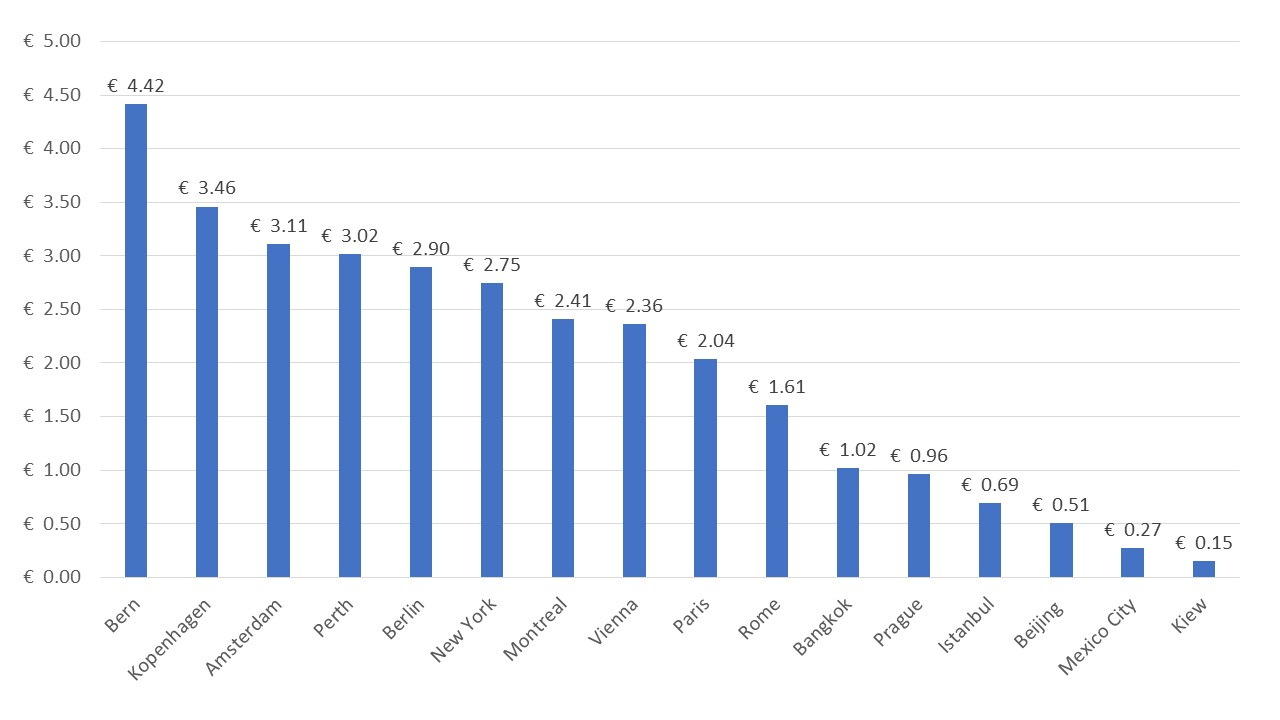
\includegraphics[width=1\linewidth]{image/tickets_prices} \caption{Preise fuer Standard-Einzelfahrscheine fuer den oeffentlichen Personennahverkehr in ausgewaehlten Staedten weltweit (statista.at, 2017)}\label{fig:unnamed-chunk-28}
\end{figure}

Immer mehr Städte bieten heutzutage den öffentlichen Verkehr komplett kostenlos an. Die ersten Versuche wurden bereits in den 1960er Jahren durchgeführt. Mittlerweile haben rund 100 Städte und Gemeinden auf der ganzen Welt den \href{https://freepublictransport.info/city/}{kostenlosen öffentlichen Verkehr} in der einen oder anderen Form eingeführt. In einigen Städten ist nur ein Teil des öffentlichen Verkehrsnetzes kostenlos, in anderen dürfen bestimmte Bevölkerungsgruppen, z. B. gemeldete Einwohner:innen oder Rentner, umsonst fahren. In Tallinn, der Hauptstadt Estlands, können die Einwohner:innen beispielsweise seit 2013 die öffentlichen Verkehrsmittel ohne Fahrschein nutzen. Laut einer Studie führte dies zu einem Anstieg des Anteils der Menschen, die öffentliche Verkehrsmittel in der Stadt nutzen, von 55 auf 63 Prozent (Cats et al., 2017). Im Jahr 2018 wurde das Modell auf andere Teile des Landes ausgeweitet. Luxemburg mit seinen 626.000 Einwohner:innenn ist das erste Land, das ab 2020 einen komplett kostenlosen öffentlichen Nahverkehr anbietet (Yeung, 2021). In Dünkirchen, Frankreich, ist der öffentliche Nahverkehr seit 2018 kostenlos. Eine von der Regierung in Auftrag gegebene Studie kam zu dem Schluss, dass acht Monate nach Einführung des Modells die Fahrten mit dem Bus unter der Woche um 65 Prozent und am Wochenende um 125 Prozent gestiegen sind. Nun experimentieren auch einige größere französische Städte mit dieser Idee. In Paris wurde im Jahr 2020 die kostenlose Nutzung des öffentlichen Nahverkehrs für unter 18-Jährige eingeführt. In Straßburg wird die gleiche Politik im September 2021 umgesetzt. Nach Angaben der Straßburger Regierung handelt es sich dabei um eine Klimaschutzmaßnahme, da viele der rund 80.000 Schulkinder derzeit von ihren Eltern zur Schule gebracht werden. Sie soll auch sozial benachteiligten Familien helfen (die mit zwei Kindern rund 550 Euro pro Jahr sparen) (Pallinger, 2021). In der südfranzösischen Region Okzitanien (mit rund sechs Millionen Einwohner:innenn) wurde ein System eingeführt, bei dem 18- bis 26-Jährige, die mindestens 30 Mal im Monat mit dem Zug fahren, nichts bezahlen müssen, mit dem doppelten Ziel, junge Arbeitnehmer zu unterstützen und die Kohlenstoffemissionen zu verringern (Yeung, 2021).

Die Kritik an kostenlosen öffentlichen Verkehrsmitteln besteht zum einen darin, dass sie dann durch höhere Steuern finanziert werden müssten. Audrey Pulvar, die stellvertretende Bürgermeisterin von Paris, will die Finanzierung durch höhere Steuern auf emissionsintensive Autos und große Unternehmen wie Amazon ausgleichen. Die Kosten, die durch Verkehrsunfälle, Luftverschmutzung und Staus entstehen, können jedenfalls eingespart werden. Nach Angaben von Pulvar belaufen sich diese in der Region Paris auf zehn Milliarden Euro pro Jahr (Pallinger, 2021). Pulvars Vorschläge sehen vor, dass zunächst Jugendliche unter 18 Jahren, Studenten und Arbeitssuchende schrittweise kostenlos befördert werden, bevor das Angebot bis 2026 auf alle Einwohner:innen an Wochenenden und dann täglich ausgeweitet wird (Yeung, 2021).

Es gibt jedoch einige Leute, die dieser Idee skeptisch gegenüberstehen. Einer von ihnen ist Kay Axhausen (Professor für Verkehrsplanung an der ETH Zürich). Er argumentiert, dass dies zu einer Überlastung des öffentlichen Verkehrs führen kann, was wiederum zu überfüllten und unzuverlässigen öffentlichen Verkehrsmitteln führt, und dass die Kund:innen wahrscheinlich zwei Tage später wieder weg sind. Prof.~Axhausen plädiert für bessere Anschlüsse, leichteres Umsteigen, Vorrangschaltung an Ampeln, mehr Busspuren und Änderungen im Streckennetz, um den öffentlichen Verkehr attraktiver zu machen (Raaflaub, 2020).

Weitere Kritikpunkte sind der Rebound-Effekt, der dazu führen könnte, dass die Menschen übermäßig viel mit Bussen und Stadtbahnen fahren, was letztlich zu einer Zunahme des Verkehrs, der Emissionen und der Zersiedelung der Landschaft führt, sowie die Befürchtung, dass sich die Qualität des öffentlichen Verkehrs verschlechtern könnte (mehr Umweltverschmutzung durch überfüllte Busse und Stadtbahnen). Ein weiterer Kritikpunkt ist, dass Studien zu dem Schluss kommen, dass nur wenige Personen, die zuvor mit dem Auto unterwegs waren, anschließend auf den kostenlosen öffentlichen Verkehr umgestiegen sind. Einer anderen Studie zufolge waren die meisten der zusätzlichen ÖPNV-Nutzer:innen vor allem Fußgänger:innen, Radfahrer:innen und Menschen, die vorher generell weniger unterwegs waren. Das Gleiche gilt für Tallinn, wo der öffentliche Verkehr zwar von 55 auf 63 Prozent zugenommen hat, der Anteil des Autoverkehrs aber nur von 31 auf 28 Prozent gesunken ist, während der Fußgängeranteil von 12 auf 7 Prozent zurückgegangen ist. Der Studie zufolge würde ein kostenloser öffentlicher Verkehr das Mobilitätsverhalten von Auto- und Motorradfahrern kaum ändern (Pallinger, 2021). Eine andere Studie in Frankreich kommt zu dem Schluss, dass die Maßnahme zwar die Fahrgastzahlen um 6 bis 10 Prozent erhöhen würde, aber zwischen 2,2 und 3,3 Milliarden Euro kosten würde, die Servicequalität des Netzes beeinträchtigt würde, die Autonutzung nur um 2 Prozent zurückginge und die Auswirkungen auf die soziale Gerechtigkeit begrenzt wären, da mehr als eine Million Menschen in der untersuchten Region bereits von kostenlosen oder ermäßigten Fahrpreisen profitieren (Mabill \& Dugue, 2018). Eine größere Veränderung könnte nach Ansicht einiger Experten durch Maßnahmen wie höhere Parkgebühren oder Kraftstoffpreise herbeigeführt werden. Anstelle einer allgemeinen Fahrscheinbefreiung könnten ärmere Bevölkerungsgruppen auch direkt unterstützt werden, beispielsweise durch günstigere Fahrscheine für einkommensschwache Haushalte. Auf diese Weise bliebe der Regierung oder dem öffentlichen Verkehrsunternehmen der größte Teil der Einnahmen aus dem Fahrkartenverkauf erhalten (Pallinger, 2021). Die Befürworter:innen eines kostenlosen öffentlichen Verkehrs in Frankreich sind jedoch der Meinung, dass die Kosten überschätzt werden, und verweisen auf eine Steuer (die so genannte Mobilitätssteuer), die von allen Unternehmen in Frankreich erhoben wird. Diese subventioniert den kollektiven Verkehr und führt dazu, dass der Fahrkartenverkauf in den meisten Städten nur etwa 10-15 \% der Einnahmen ausmacht. Im Fall von Dünkirchen deckte diese Steuer die Kosten für die Abschaffung der Fahrkartenpreise, die 10 \% der Einnahmen ausmachten (Yeung, 2021).

\hypertarget{relevante-initiativen-in-uxf6sterreich-23}{%
\subsection*{Relevante Initiativen in Österreich}\label{relevante-initiativen-in-uxf6sterreich-23}}
\addcontentsline{toc}{subsection}{Relevante Initiativen in Österreich}

The government in Austria is committed to the implementation of the so-called Climate ticket, which should make ticket prices cheaper in the future.

\begin{itemize}
\tightlist
\item
  \href{https://www.bmk.gv.at/themen/mobilitaet/1-2-3-ticket.html}{BMK.gv.at}
\end{itemize}

\hypertarget{auswirkungen-in-bezug-auf-die-ziele-fuxfcr-nachhaltige-entwicklung-sdgs-23}{%
\subsection*{Auswirkungen in Bezug auf die Ziele für nachhaltige Entwicklung (SDGs)}\label{auswirkungen-in-bezug-auf-die-ziele-fuxfcr-nachhaltige-entwicklung-sdgs-23}}
\addcontentsline{toc}{subsection}{Auswirkungen in Bezug auf die Ziele für nachhaltige Entwicklung (SDGs)}

\begin{longtable}[]{@{}ccccc@{}}
\toprule
\begin{minipage}[b]{0.17\columnwidth}\centering
Ebene der Auswirkungen\strut
\end{minipage} & \begin{minipage}[b]{0.16\columnwidth}\centering
Indikator\strut
\end{minipage} & \begin{minipage}[b]{0.17\columnwidth}\centering
Richtung der Auswirkungen\strut
\end{minipage} & \begin{minipage}[b]{0.17\columnwidth}\centering
Beschreibung des Ziels \& SDG\strut
\end{minipage} & \begin{minipage}[b]{0.17\columnwidth}\centering
Beschreibung des Ziels \& SDG\strut
\end{minipage}\tabularnewline
\midrule
\endhead
\begin{minipage}[t]{0.17\columnwidth}\centering
Individuell\strut
\end{minipage} & \begin{minipage}[t]{0.16\columnwidth}\centering
Hoehere gesellschaftliche Gerechtigkeit und Zugaenglichkeit des oeffentlichen Verkehrs\strut
\end{minipage} & \begin{minipage}[t]{0.17\columnwidth}\centering
\textbf{+}\strut
\end{minipage} & \begin{minipage}[t]{0.17\columnwidth}\centering
Gleichheit (\emph{5,10})\strut
\end{minipage} & \begin{minipage}[t]{0.17\columnwidth}\centering
Brown, 2018; Pallinger, 2021\strut
\end{minipage}\tabularnewline
\begin{minipage}[t]{0.17\columnwidth}\centering
Individuell\strut
\end{minipage} & \begin{minipage}[t]{0.16\columnwidth}\centering
Verringerung des Anteils nachhaltiger Verkehrsmittel (z. B. zu Fuss gehen) aufgrund der verstaerkten Nutzung des kostenlosen oeffentlichen Verkehrs\strut
\end{minipage} & \begin{minipage}[t]{0.17\columnwidth}\centering
\textbf{-}\strut
\end{minipage} & \begin{minipage}[t]{0.17\columnwidth}\centering
Oekologische Nachhaltigkeit (\emph{7,12,13,15})\strut
\end{minipage} & \begin{minipage}[t]{0.17\columnwidth}\centering
Pallinger, 2021\strut
\end{minipage}\tabularnewline
\begin{minipage}[t]{0.17\columnwidth}\centering
Systemisch\strut
\end{minipage} & \begin{minipage}[t]{0.16\columnwidth}\centering
Geringere Kohlenstoffemissionen\strut
\end{minipage} & \begin{minipage}[t]{0.17\columnwidth}\centering
\textbf{+}\strut
\end{minipage} & \begin{minipage}[t]{0.17\columnwidth}\centering
Oekologische Nachhaltigkeit (\emph{7,12,13,15})\strut
\end{minipage} & \begin{minipage}[t]{0.17\columnwidth}\centering
Yeung, 2021\strut
\end{minipage}\tabularnewline
\begin{minipage}[t]{0.17\columnwidth}\centering
Systemisch\strut
\end{minipage} & \begin{minipage}[t]{0.16\columnwidth}\centering
Potenziell uebermaessige Fahrten mit oeffentlichen Verkehrsmitteln koennen deren Qualitaet beeintraechtigen\strut
\end{minipage} & \begin{minipage}[t]{0.17\columnwidth}\centering
\textbf{-}\strut
\end{minipage} & \begin{minipage}[t]{0.17\columnwidth}\centering
Nachhaltige wirtschaftliche Entwicklung (\emph{8,11})\strut
\end{minipage} & \begin{minipage}[t]{0.17\columnwidth}\centering
Raaflaub, 2020\strut
\end{minipage}\tabularnewline
\bottomrule
\end{longtable}

\hypertarget{technologie--und-gesellschaftlicher-bereitschaftsgrad-20}{%
\subsection*{Technologie- und gesellschaftlicher Bereitschaftsgrad}\label{technologie--und-gesellschaftlicher-bereitschaftsgrad-20}}
\addcontentsline{toc}{subsection}{Technologie- und gesellschaftlicher Bereitschaftsgrad}

\begin{longtable}[]{@{}cc@{}}
\toprule
Stand der Technologiebereitschaft & Gesellschaftlicher Bereitschaftsgrad\tabularnewline
\midrule
\endhead
8-9 & 7-9\tabularnewline
\bottomrule
\end{longtable}

\hypertarget{weitere-links-19}{%
\subsection*{Weitere links}\label{weitere-links-19}}
\addcontentsline{toc}{subsection}{Weitere links}

\begin{itemize}
\tightlist
\item
  \href{https://freepublictransport.info/city/}{Freepublictransport.info}
\item
  \href{https://orf.at/stories/3113027/}{Orf.at}
\end{itemize}

\hypertarget{referenzen-23}{%
\subsection*{Referenzen}\label{referenzen-23}}
\addcontentsline{toc}{subsection}{Referenzen}

\begin{itemize}
\tightlist
\item
  Krakow.pl (2021). Rodzaje biletów. Available at: \url{https://www.krakow.pl/14904,artykul,rodzaje_biletow.html}. {[}Accessed: 1st June 2021{]}
\item
  McKone, J. (2010). Time-Based Versus Distance-Based Fares. Available at: \url{https://thecityfix.com/blog/time-based-versus-distance-based-fares/\#}:\textasciitilde:text=Time\%2Dbased\%20systems\%20allow\%20passengers,a\%20set\%20amount\%20of\%20time.\&text=Distance\%2Dbased\%20systems\%20charge\%20higher,rides\%20that\%20cover\%20greater\%20distances. {[}Accessed: 1st June 2021{]}
\item
  Wiener Linien.at (2021). Ticket guide. Available at: \url{https://www.wienerlinien.at/eportal3/ep/channelView.do/pageTypeId/66533/channelId/-47643} {[}Accessed: 1st June 2021{]}
\item
  ADAC. (2019, June 19). ÖPNV-Preisvergleich 2019: Wo Tickets teuer und wo sie günstig sind \textbar{} ADAC. \url{https://www.adac.de/reise-freizeit/ratgeber/tests/oepnv-preise-vergleich/}
\item
  Brown, A. E. (2018). Fair fares? How flat and variable fares affect transit equity in Los Angeles. Case Studies on Transport Policy, 6(4), 765--773. \url{https://doi.org/10.1016/J.CSTP.2018.09.011}
\item
  Cats, O., Susilo, Y. O., \& Reimal, T. (2017). The prospects of fare-free public transport: evidence from Tallinn. Transportation, 44(5), 1083--1104. \url{https://doi.org/10.1007/s11116-016-9695-5}
\item
  Chalabianlou, R., Lawrence, A., \& Baxter, B. (2015). A review and assessment of fare capping as a passenger incentive mechanism for Australia and New Zealand. ATRF 2015 - Australasian Transport Research Forum 2015, Proceedings, October, 1--15.
\item
  El-Geneidy, A., Levinson, D., Diab, E., Boisjoly, G., Verbich, D., \& Loong, C. (2016). The cost of equity: Assessing transit accessibility and social disparity using total travel cost. Transportation Research Part A: Policy and Practice, 91, 302--316. \url{https://doi.org/10.1016/j.tra.2016.07.003}
\item
  Guzman, L. A., de la Hoz, D., \& Monzón, A. (2014). Optimal and Long-Term Dynamic Transport Policy Design: Seeking Maximum Social Welfare through a Pricing Scheme. International Journal of Sustainable Transportation, 8(4), 297--316. \url{https://doi.org/10.1080/15568318.2012.696772}
\item
  Los Angeles County Metropolitan Transportation Authority. (2021). LA Metro Rider Relief. \url{https://www.metro.net/projects/rider_relief/}
\item
  Mabill, S., \& Dugue, H. (2018). Rapport du Comité sur la faisabilité de la gratuité des transports en commun en Île-de-France, leur financement et la politique de tarification. 2018--2019. \url{https://www.iledefrance-mobilites.fr/wp-content/uploads/2018/10/Rapport-Comité-sur-la-faisabilité-de-la-gratuité-des-transports-en-commun-en-Île-de-France-leur-financement-et-la-politique-de-tarification.pdf}
\item
  Martens, K. (2012). Justice in transport as justice in accessibility: Applying Walzer's ``Spheres of Justice'' to the transport sector. Transportation, 39(6), 1035--1053. \url{https://doi.org/10.1007/s11116-012-9388-7}
\item
  Pallinger, J. (2021, June 5). Was kostenlose Öffis bringen sollen - Zukunft - derStandard.de › Wissen und Gesellschaft. \url{https://www.derstandard.de/story/2000127046621/was-kostenlose-oeffis-bringen-sollen}
\item
  Raaflaub, C. (2020, February 27). Warum die Idee vom Gratis-ÖV in der Schweiz nicht ankommt - SWI swissinfo.ch. \url{https://www.swissinfo.ch/ger/verkehr-und-umweltschutz_warum-die-idee-vom-gratis-oev-in-der-schweiz-nicht-ankommt/45578796}
\item
  Rubensson, I., Susilo, Y., \& Cats, O. (2020). Is flat fare fair? Equity impact of fare scheme change. Transport Policy, 91, 48--58. \url{https://doi.org/10.1016/J.TRANPOL.2020.03.013}
\item
  San Francisco Municipal Transportation Agency. (2021, January). Lifeline Pass \textbar{} SFMTA. \url{https://www.sfmta.com/fares/lifeline-pass}
\item
  statista.at. (2017, April). ÖPNV - Preise für Standard-Einzeltickets weltweit 2017 \textbar{} Statista. \url{https://de.statista.com/statistik/daten/studie/168444/umfrage/preise-fuer-standard-einzeltickets-des-oepnv-in-ausgewaehlten-staedten/}
\item
  Streeting, M., \& Charles, P. (2006). Developments in transit fare policy reform. 29th Australasian Transport Research Forum, ATRF 06, 1--13.
\item
  Wang, S., Liu, Y., \& Corcoran, J. (2021). Equity of public transport costs before and after a fare policy reform: An empirical evaluation using smartcard data. Transportation Research Part A: Policy and Practice, 144, 104--118. \url{https://doi.org/10.1016/J.TRA.2020.12.010}
\item
  Yeung, P. (2021, May 24). How France is testing free public transport - BBC Worklife. \url{https://www.bbc.com/worklife/article/20210519-how-france-is-testing-free-public-transport}
\item
  Yoh, A. C., Taylor, B. D., \& Gahbauer, J. (2016). Does Transit Mean Business? Reconciling Economic, Organizational, and Political Perspectives on Variable Transit Fares. Public Works Management and Policy, 21(2), 157--172. \url{https://doi.org/10.1177/1087724X15616816}
\item
  Zhao, P., \& Zhang, Y. (2019). The effects of metro fare increase on transport equity: New evidence from Beijing. Transport Policy, 74, 73--83. \url{https://doi.org/10.1016/J.TRANPOL.2018.11.009}
\end{itemize}

\hypertarget{maas}{%
\section{Mobilität als Dienstleistung - Mobility as a service (Maas)}\label{maas}}

\hypertarget{synonyme-20}{%
\subsection*{Synonyme}\label{synonyme-20}}
\addcontentsline{toc}{subsection}{Synonyme}

\emph{\href{http://changemobility.at/wiki/index.php?title=MaaS_-_Mobility_as_a_Service}{MaaS}}

\hypertarget{definition-24}{%
\subsection*{Definition}\label{definition-24}}
\addcontentsline{toc}{subsection}{Definition}

Nach dem Prinzip ``Nutzen statt Besitzen'' ist ein Ziel von MaaS, Mobilität als Dienstleistung jederzeit und überall mit einem Klick auf einer oder mehreren Online-Plattformen oder Apps verfügbar zu machen. Diese digitalen MaaS-Plattformen oder -Apps sollen Information, Buchung und Bezahlung von Mobilitätsangeboten verschiedener Dienstleister miteinander verknüpfen und so das Angebot von integrierten Mobilitätspaketen ermöglichen. Die Nutzer:innen sollten die Freiheit haben, zwischen verschiedenen physischen Mobilitätsformen zu wählen (Neumann \& Rauch, 2021):
- öffentliche Verkehrsmittel wie Zug, Bus, S-Bahn, Stadtbahn und U-Bahn
- private Dienstleistungen wie Taxis
- Dienste für Car-, Ride-, (E-)Bike-, (E-)Scooter-Sharing oder Linientaxis
- ehrenamtlich betriebene Gemeindebusse
- Flugzeuge und Schiffe
- (in Zukunft) automatisierte, fahrerlose Fahrzeuge
MaaS-Lösungen können in mehreren Stufen aufgebaut werden. Die erste Stufe besteht aus einer Bündelung von Informationen verschiedener Anbieter, so dass alle verfügbaren Mobilitätsangebote für die gesamte Strecke von Start bis Ziel angezeigt werden. Die zweite Stufe umfasst die Routenplanung nach den Prioritäten der Kund:innen und die Möglichkeit, alle für die Fahrt genutzten Verkehrsmittel auf einmal zu buchen und zu bezahlen. Hinzu kommen Echtzeitinformationen für die Strecke, wie z.B. Änderungen der Fahr- und Wartezeiten aufgrund unvorhergesehener Ereignisse - wie z.B. Unfälle oder Wetterbedingungen - sowie kontinuierliche Hinweise auf alternative Möglichkeiten. Die dritte Stufe besteht in einer Mobilitätsgarantie durch ein auf die persönlichen Bedürfnisse und Präferenzen zugeschnittenes Mobilitätspaket, z.B. in Form eines Monatsabonnements (Neumann \& Rauch, 2021).
Ziel von MaaS ist es, eine Alternative zur privaten Autonutzung zu bieten, die ebenso bequem, sogar billiger, aber nachhaltiger ist (Maas Alliance, 2015). Die Theorie von MaaS eröffnet neue Geschäftsfelder und ermöglicht es Mobilitätsdienstleistern, ihren Kundenstamm zu vergrößern. Die durch den laufenden Betrieb generierten Nutzungsdaten können dazu beitragen, die Kund:innen besser kennenzulernen und somit effizienter zu arbeiten, da die Ausrichtung und Verteilung der Dienste besser geplant werden kann. Ein gut funktionierendes MaaS-System erfordert die Bereitschaft privater und öffentlicher Mobilitätsanbieter zur Kooperation untereinander und mit den Plattformbetreibern (MaaS-Anbietern) (Neumann \& Rauch, 2021). Darüber hinaus hängt es stark von der Verfügbarkeit hochwertiger Daten ab. Die Durchsetzung eines sicheren Echtzeitzugangs zu den Daten ist ebenso wichtig wie die Gewährleistung der Klarheit über die Haftung der Parteien, die die Hauptkontrolle über die Daten haben (Maas Alliance, 2015). Der erste Schritt auf dem Weg zu MaaS ist die Harmonisierung von Daten, unterstützt durch geeignete Vorschriften und Standards (Maas Alliance, 2015). In Österreich forschen sowohl Forscher:innen als auch Mobilitätsdienstleister daran, wie man MaaS am besten umsetzen kann. Ein Beispiel dafür ist das Forschungsprojekt ULTIMOB.

\hypertarget{wichtige-interessensgruppen-24}{%
\subsection*{Wichtige Interessensgruppen}\label{wichtige-interessensgruppen-24}}
\addcontentsline{toc}{subsection}{Wichtige Interessensgruppen}

\begin{itemize}
\tightlist
\item
  \textbf{Betroffene}: Kund:innen/Benutzer:innen
\item
  \textbf{Verantwortliche}: Verkehrsdienstleister und Betreiber öffentlicher Verkehrsmittel, MaaS-Betreiber und -Integratoren, IT-Systemanbieter, Stadtverwaltungen, lokale, regionale und nationale Behörden
\end{itemize}

\hypertarget{aktueller-stand-der-wissenschaft-und-forschung-24}{%
\subsection*{Aktueller Stand der Wissenschaft und Forschung}\label{aktueller-stand-der-wissenschaft-und-forschung-24}}
\addcontentsline{toc}{subsection}{Aktueller Stand der Wissenschaft und Forschung}

Um die Zusammenarbeit zwischen privaten und öffentlichen Mobilitätsanbietern sowie Plattformbetreibern (MaaS-Anbietern) zu unterstützen, sollten auf europäischer und österreichischer Ebene die rechtlichen und organisatorischen Rahmenbedingungen sowie Standards für einen sicheren und fairen Datenaustausch geschaffen werden (Neumann \& Rauch, 2021).
Im Jahr 2015 wurde die MaaS Alliance gegründet, eine öffentlich-private Partnerschaft, die daran arbeitet, Grundlagen für einen gemeinsamen Ansatz für MaaS zu schaffen, mit dem Hauptziel, einen einheitlichen, offenen Markt und die vollständige Einführung von MaaS-Diensten zu ermöglichen (Maas Alliance, 2015).
Das Forschungs- und Entwicklungsprojekt MaaS4EU, das durch das Forschungs- und Innovationsprogramm Horizon2020 finanziert wird, bringt 17 Partner aus verschiedenen Sektoren und mit unterschiedlichem Hintergrund zusammen, um praktikable Beweise und Lösungen für das MaaS-Konzept zu liefern. Das Projekt zielt darauf ab, Hindernisse zu beseitigen und einen kooperativen und vernetzten EU-Binnenmarkt für das MaaS-Konzept zu ermöglichen, indem es sich mit den vier Säulen befasst:

\begin{enumerate}
\def\labelenumi{(\arabic{enumi})}
\tightlist
\item
  Geschäftsmodelle
\item
  Endnutzer:innen
\item
  Technologie
\item
  Politik
\end{enumerate}

Daher werden die ganzheitlichen MaaS4EU-Lösungen in Living Labs im Großraum Manchester (UK), in Luxemburg (Deutschland) und in Budapest (Ungarn) demonstriert und in der Praxis validiert (MaaS4EU, 2017). Zusammenfassend lässt sich sagen, dass die aktuelle Forschung hauptsächlich an der Entwicklung verschiedener Prototypen von MaaS-Apps/Plattformen arbeitet, die eine multimodale Reiselösung bieten sollen. Ein Beispiel ist das Projekt \emph{TrønderMaaS} von Marinelli et al.~(2020), das einen groß angelegten Pilotversuch in der Region Trondheim-Stjørdal, Norwegen, durchführt.

\hypertarget{aktueller-stand-der-praktischen-umsetzung-24}{%
\subsection*{Aktueller Stand der praktischen Umsetzung}\label{aktueller-stand-der-praktischen-umsetzung-24}}
\addcontentsline{toc}{subsection}{Aktueller Stand der praktischen Umsetzung}

Im Jahr 2019 haben die \emph{zusammen mit dem litauischen Start-up und MaaS-Lösungsanbieter }Trafi* die Mobilitäts-App \emph{Jelbi}, entwickelt und implementiert, die als weltweit umfangreichste Mobility-as-a-Service-Lösung gilt (Rastenyt?, 2020). Die App umfasst Assistenzplanung und Routenfindung, Echtzeit-Informationen über den öffentlichen Nahverkehr und den Standort und die Verfügbarkeit von Shared-Mobility-Fahrzeugen, eine optimierte Zahlungslösung für jeden integrierten Mobilitätsdienst sowie die Möglichkeit, die Dauer und Kosten jeder Fahrt zu vergleichen (Rastenyt?, 2020).

Im Jahr 2020 folgte die Schweiz und integrierte eine App namens \emph{yumuv}. \emph{Schweizerischen Bundesbahnen SBB CFF FFS, PTOs of Verkehrsbetriebe Zürich, Basler Verkehrs-Betriebe (BVB)}, und \emph{BERNMOBIL} ckooperierten ebenfalls mit dem Start-up \emph{Trafi} und schafften es, das erste regionale MaaS mit Abonnements zu schaffen (Trafi Ltd., 2020).

\hypertarget{relevante-initiativen-in-uxf6sterreich-24}{%
\subsection*{Relevante Initiativen in Österreich}\label{relevante-initiativen-in-uxf6sterreich-24}}
\addcontentsline{toc}{subsection}{Relevante Initiativen in Österreich}

\begin{itemize}
\tightlist
\item
  \href{https://www.austriatech.at/assets/Uploads/Publikationen/PDF-Dateien/29fc02ada2/MaaS-miA_english_102019_web.pdf}{AustriaTech.at}
\item
  \href{https://maas-ready.at}{maas-ready.at}
\item
  \href{https://www.ultimob.at}{ultimob.at}
\item
  \href{https://www.tim-oesterreich.at/graz/}{tim-oesterreich.at}
\item
  \href{https://wegfinder.at/}{wegfinder.at}
\item
  \href{https://www.wienerlinien.at/eportal3/ep/channelView.do/pageTypeId/66526/channelId/-3600060}{wienerlinien.at}
\item
  \href{https://anachb.vor.at/}{anachb.vor.at}
\end{itemize}

\hypertarget{auswirkungen-in-bezug-auf-die-ziele-fuxfcr-nachhaltige-entwicklung-sdgs-24}{%
\subsection*{Auswirkungen in Bezug auf die Ziele für nachhaltige Entwicklung (SDGs)}\label{auswirkungen-in-bezug-auf-die-ziele-fuxfcr-nachhaltige-entwicklung-sdgs-24}}
\addcontentsline{toc}{subsection}{Auswirkungen in Bezug auf die Ziele für nachhaltige Entwicklung (SDGs)}

\begin{longtable}[]{@{}ccccc@{}}
\toprule
\begin{minipage}[b]{0.17\columnwidth}\centering
Ebene der Auswirkungen\strut
\end{minipage} & \begin{minipage}[b]{0.16\columnwidth}\centering
Indikator\strut
\end{minipage} & \begin{minipage}[b]{0.17\columnwidth}\centering
Richtung der Auswirkungen\strut
\end{minipage} & \begin{minipage}[b]{0.17\columnwidth}\centering
Beschreibung des Ziels \& SDG\strut
\end{minipage} & \begin{minipage}[b]{0.17\columnwidth}\centering
Beschreibung des Ziels \& SDG\strut
\end{minipage}\tabularnewline
\midrule
\endhead
\begin{minipage}[t]{0.17\columnwidth}\centering
Individuell\strut
\end{minipage} & \begin{minipage}[t]{0.16\columnwidth}\centering
Erleichterte Zugaenglichkeit zum Verkehr\strut
\end{minipage} & \begin{minipage}[t]{0.17\columnwidth}\centering
\textbf{+}\strut
\end{minipage} & \begin{minipage}[t]{0.17\columnwidth}\centering
Gleichheit (\emph{5,10})\strut
\end{minipage} & \begin{minipage}[t]{0.17\columnwidth}\centering
Gudonavicius, 2020\strut
\end{minipage}\tabularnewline
\begin{minipage}[t]{0.17\columnwidth}\centering
Individuell\strut
\end{minipage} & \begin{minipage}[t]{0.16\columnwidth}\centering
Hoehere Nutzung aktiver Verkehrsmittel/geringerer Kraftstoffverbrauch\strut
\end{minipage} & \begin{minipage}[t]{0.17\columnwidth}\centering
\textbf{+}\strut
\end{minipage} & \begin{minipage}[t]{0.17\columnwidth}\centering
Oekologische Nachhaltigkeit (\emph{7,12,13,15})\strut
\end{minipage} & \begin{minipage}[t]{0.17\columnwidth}\centering
Gudonavicius, 2020\strut
\end{minipage}\tabularnewline
\begin{minipage}[t]{0.17\columnwidth}\centering
Individuell\strut
\end{minipage} & \begin{minipage}[t]{0.16\columnwidth}\centering
Bessere Erreichbarkeit und kuerzere Reisezeit\strut
\end{minipage} & \begin{minipage}[t]{0.17\columnwidth}\centering
\textbf{+}\strut
\end{minipage} & \begin{minipage}[t]{0.17\columnwidth}\centering
Nachhaltige wirtschaftliche Entwicklung (\emph{8,11})\strut
\end{minipage} & \begin{minipage}[t]{0.17\columnwidth}\centering
Gudonavicius, 2020; Marinelli et al., 2020\strut
\end{minipage}\tabularnewline
\begin{minipage}[t]{0.17\columnwidth}\centering
Individuell\strut
\end{minipage} & \begin{minipage}[t]{0.16\columnwidth}\centering
Nutzung des digitalisierten Verkehrs\strut
\end{minipage} & \begin{minipage}[t]{0.17\columnwidth}\centering
\textbf{+}\strut
\end{minipage} & \begin{minipage}[t]{0.17\columnwidth}\centering
Innovation und Infrastruktur (\emph{9})\strut
\end{minipage} & \begin{minipage}[t]{0.17\columnwidth}\centering
Gudonavicius, 2020; Marinelli et al., 2020\strut
\end{minipage}\tabularnewline
\begin{minipage}[t]{0.17\columnwidth}\centering
Systemisch\strut
\end{minipage} & \begin{minipage}[t]{0.16\columnwidth}\centering
Erhoehung der Verkehrssicherheit/Verringerung der Kollisionsrate\strut
\end{minipage} & \begin{minipage}[t]{0.17\columnwidth}\centering
\textbf{+}\strut
\end{minipage} & \begin{minipage}[t]{0.17\columnwidth}\centering
Gesundheit und Wohlbefinden (\emph{3})\strut
\end{minipage} & \begin{minipage}[t]{0.17\columnwidth}\centering
Gudonavicius, 2020; Marinelli et al., 2020\strut
\end{minipage}\tabularnewline
\begin{minipage}[t]{0.17\columnwidth}\centering
Systemisch\strut
\end{minipage} & \begin{minipage}[t]{0.16\columnwidth}\centering
Verringerung der Emissionsrate\strut
\end{minipage} & \begin{minipage}[t]{0.17\columnwidth}\centering
\textbf{+}\strut
\end{minipage} & \begin{minipage}[t]{0.17\columnwidth}\centering
Oekologische Nachhaltigkeit (\emph{7,12,13,15})\strut
\end{minipage} & \begin{minipage}[t]{0.17\columnwidth}\centering
Gudonavicius, 2020\strut
\end{minipage}\tabularnewline
\begin{minipage}[t]{0.17\columnwidth}\centering
Systemisch\strut
\end{minipage} & \begin{minipage}[t]{0.16\columnwidth}\centering
Effizienz des Verkehrs\strut
\end{minipage} & \begin{minipage}[t]{0.17\columnwidth}\centering
\textbf{+}\strut
\end{minipage} & \begin{minipage}[t]{0.17\columnwidth}\centering
Nachhaltige wirtschaftliche Entwicklung (\emph{8,11})\strut
\end{minipage} & \begin{minipage}[t]{0.17\columnwidth}\centering
Gudonavicius, 2020\strut
\end{minipage}\tabularnewline
\begin{minipage}[t]{0.17\columnwidth}\centering
Systemisch\strut
\end{minipage} & \begin{minipage}[t]{0.16\columnwidth}\centering
Effizienz von Verkehrssystemen, erhoehte Widerstandsfaehigkeit durch Echtzeitdaten\strut
\end{minipage} & \begin{minipage}[t]{0.17\columnwidth}\centering
\textbf{+}\strut
\end{minipage} & \begin{minipage}[t]{0.17\columnwidth}\centering
Innovation und Infrastruktur (\emph{9})\strut
\end{minipage} & \begin{minipage}[t]{0.17\columnwidth}\centering
Marinelli et al., 2020\strut
\end{minipage}\tabularnewline
\begin{minipage}[t]{0.17\columnwidth}\centering
Systemisch\strut
\end{minipage} & \begin{minipage}[t]{0.16\columnwidth}\centering
Zusammenarbeit von privatem und oeffentlichem Sektor \& globale Partnerschaften\strut
\end{minipage} & \begin{minipage}[t]{0.17\columnwidth}\centering
\textbf{+}\strut
\end{minipage} & \begin{minipage}[t]{0.17\columnwidth}\centering
Partnerschaften und Kooperationen (\emph{17})\strut
\end{minipage} & \begin{minipage}[t]{0.17\columnwidth}\centering
Gudonavicius, 2020; Marinelli et al., 2020\strut
\end{minipage}\tabularnewline
\bottomrule
\end{longtable}

\hypertarget{technologie--und-gesellschaftlicher-bereitschaftsgrad-21}{%
\subsection*{Technologie- und gesellschaftlicher Bereitschaftsgrad}\label{technologie--und-gesellschaftlicher-bereitschaftsgrad-21}}
\addcontentsline{toc}{subsection}{Technologie- und gesellschaftlicher Bereitschaftsgrad}

\begin{longtable}[]{@{}cc@{}}
\toprule
Stand der Technologiebereitschaft & Gesellschaftlicher Bereitschaftsgrad\tabularnewline
\midrule
\endhead
3-7 & 5-7\tabularnewline
\bottomrule
\end{longtable}

\hypertarget{offene-fragen-22}{%
\subsection*{Offene Fragen}\label{offene-fragen-22}}
\addcontentsline{toc}{subsection}{Offene Fragen}

\begin{enumerate}
\def\labelenumi{\arabic{enumi}.}
\tightlist
\item
  Wie kann eine Nachhaltigkeitstransformation durch MaaS erreicht werden und welche Voraussetzungen braucht es dafür?
\item
  Wie kann der Datenschutz beim Einsatz von MaaS gewährleistet werden?
\item
  Wie schnell kann MaaS umgesetzt werden?
\item
  Wie können bürokratische Hürden zeitnah überwunden werden?
\end{enumerate}

\hypertarget{weitere-links-20}{%
\subsection*{Weitere links}\label{weitere-links-20}}
\addcontentsline{toc}{subsection}{Weitere links}

\begin{itemize}
\tightlist
\item
  \href{https://maas-alliance.eu/wp-content/uploads/sites/7/2017/09/MaaS-WhitePaper_final_040917-2.pdf}{maas-alliance.eu}
\item
  \href{https://www.trafi.com}{trafi.com}
\item
  \href{https://www.jelbi.de}{jelbi.de}
\item
  \href{https://www.ubigo.me/en/about-ubigo}{ubigo.me}
\item
  \href{http://www.maas4eu.eu}{maas4eu.eu}
\end{itemize}

\hypertarget{referenzen-24}{%
\subsection*{Referenzen}\label{referenzen-24}}
\addcontentsline{toc}{subsection}{Referenzen}

\begin{itemize}
\tightlist
\item
  Gudonavičius, M. (2020). Unjamming Urban Mobility: How Mobility-as-a-Service Can Replace Personal Cars. \url{https://www.trafi.com/wp-content/uploads/2020/08/unjamming-urban-mobility.pdf} - Maas Alliance. (2015). White Paper: Guidelines \& Recommendations to create the foundation for a thriving MaaS Ecosystem. 32(2), 1--27. \url{https://maas-alliance.eu/wp-content/uploads/sites/7/2017/09/MaaS-WhitePaper_final_040917-2.pdf}
\item
  MaaS4EU. (2017, October). Launch of MaaS4EU project. \url{http://www.maas4eu.eu/wp-content/uploads/2017/10/MaaS4EU-Launch-Press-Release.pdf}
\item
  Marinelli, G., Nordfjærn, Ö. S., Aarseth, W., \& Pitera, K. (2020). Introducing TrønderMaaS: investigating business models, sustainability and users' acceptance of a MaaS system in Stjørdal and Trondheim region, Norway.
\item
  Neumann, A., \& Rauch, A. (2021). Maas Ready. \url{https://maas-ready.at/allgemein\#Grundidee}
\item
  Rastenytė, J. (2020, April 24). BVG Jelbi -- Case Study: World's Most Extensive MaaS in Berlin -- Trafi. \url{https://www.trafi.com/bvg-jelbi-maas-berlin/}
\item
  Trafi Ltd.~(2020). yumuv -- Regional MaaS with subscriptions in Switzerland -- Trafi. \url{https://www.trafi.com/yumuv/}
\end{itemize}

\hypertarget{p_r}{%
\section{Park and ride}\label{p_r}}

\hypertarget{synonyms-1}{%
\subsection*{Synonyms}\label{synonyms-1}}
\addcontentsline{toc}{subsection}{Synonyms}

\emph{P\&R, P and R, P+R}

\hypertarget{definition-25}{%
\subsection*{Definition}\label{definition-25}}
\addcontentsline{toc}{subsection}{Definition}

Einige der größten Herausforderungen, mit denen die Welt derzeit konfrontiert ist, stehen im Zusammenhang mit dem Bevölkerungswachstum und der Urbanisierung. Das massive Wachstum der Städte hat zu großen Herausforderungen im Verkehrswesen geführt, die sich in Verkehrsstaus in städtischen Gebieten, insbesondere in den Stadtzentren, äußern. Viele der Bemühungen zur Verringerung der Verkehrsüberlastung zielen darauf ab, die Fahrzeugauslastung zu erhöhen, indem sie eine Verlagerung von Einzelfahrzeugen auf Mehrzweckfahrzeuge bewirken oder die Nutzung verschiedener Verkehrsmittel fördern. Ein Beispiel für solche Bemühungen sind Park-and-Ride-Anlagen, mit denen versucht wird, die Autonutzung zu verringern und die Effizienz der Straßen zu steigern.
Park-and-Ride-Anlagen befinden sich in der Regel in Stadtrandgebieten in der Nähe von Bus- oder Bahnhöfen, damit Autofahrer:innen, die aus Vororten oder ländlichen Gebieten kommen, ihr Fahrzeug abstellen und auf öffentliche Verkehrsmittel umsteigen können, um städtische Ziele zu erreichen. Park-and-Ride-Anlagen, die in den 1970er Jahren in England eingeführt wurden, scheinen eine einfache und kostengünstige Alternative zum Bau neuer Straßen zu sein. Diese Anlagen werden in der Regel von guten öffentlichen Verkehrsdiensten in städtische Gebiete begleitet (Katoshevski-Cavari, Bak und Shiftan, 2018).

\hypertarget{wichtige-interessensgruppen-25}{%
\subsection*{Wichtige Interessensgruppen}\label{wichtige-interessensgruppen-25}}
\addcontentsline{toc}{subsection}{Wichtige Interessensgruppen}

\begin{itemize}
\tightlist
\item
  \textbf{Betroffene}: Autofahrer:innen, die aus Vorstädten und ländlichen Gebieten kommen
\item
  \textbf{Verantwortliche}: Nationale Regierungen, Kommunalverwaltungen, Stadtverwaltungen, Parkraumbewirtschaftungsunternehmen
\end{itemize}

\hypertarget{aktueller-stand-der-wissenschaft-und-forschung-25}{%
\subsection*{Aktueller Stand der Wissenschaft und Forschung}\label{aktueller-stand-der-wissenschaft-und-forschung-25}}
\addcontentsline{toc}{subsection}{Aktueller Stand der Wissenschaft und Forschung}

Im Bereich der P\&R-Forschung befassen sich die vorhandenen Veröffentlichungen mit Themen wie dem Problem der optimalen Lage von P\&R-Anlagen, dem Zusammenhang zwischen dem Nutzungsverhalten von Privatfahrzeugen und der Anzahl und Dichte von P\&R-Anlagen in einer Stadt, der empirischen Untersuchung des Nutzungsverhaltens von P\&R-Anlagen, der Untersuchung von P\&R-Motiven und Luftqualitätsstandards in Europa, der Einfluss von P\&R-Anlagen auf die zurückgelegten Fahrzeugkilometer, die Analyse der erklärten Absicht von Reisenden, Park- und Radverkehrsanlagen (P+R, B+R) zu nutzen, die empirische Analyse des Wahlverhaltens von P\&R-Anlagen, Einstellungserhebungen von P\&R- und Nicht-P\&R-Nutzer:innen und der Einfluss multimodaler Informationen auf die Nutzung von P\&R (Gan und Ye, 2018).
Studien zeigen, dass einige ÖPNV-Nutzer:innen zum Umstieg auf mehrere Verkehrsmittel (z. B. Park-and-Ride) bewegt wurden, was die Zahl der Autofahrten erhöhte. Nichtsdestotrotz werden zusätzliche Autofahrten in nicht überlasteten Gebieten unternommen, was zur Verkehrsentlastung beiträgt (Katoshevski-Cavari, Bak und Shiftan, 2018).
Die genauen Auswirkungen von P\&R sind umstritten. Einige Studien haben bestätigt, dass P\&R-Einrichtungen die Nutzung öffentlicher Verkehrsmittel fördern, den städtischen Verkehr entlasten und die Pkw-Emissionen in Stadtzentren verringern können. Andere Studien wiesen auf mögliche Gegeneffekte von P\&R hin. Die Verringerung der Staus in den Stadtzentren könnte Autofahrer:innen ermutigen, wieder mit dem Auto in die Stadt zu fahren, da sich die Erreichbarkeit verbessert hat, und Autofahrer:innen, die über P\&R-Anlagen ins Stadtzentrum fahren, könnten einige zusätzliche Kilometer zurücklegen, um die P\&R-Anlage zu erreichen. Das genaue Gewicht dieser negativen externen Effekte ist noch umstritten (und wird von Ort zu Ort variieren), ebenso wie der direkte Nettonutzen von P\&R für den Autoverkehr im Stadtgebiet insgesamt. Es ist jedoch unbestritten, dass gut genutzte P\&R-Anlagen den Autoverkehr im Stadtzentrum direkt reduzieren (Dijk und Montalvo, 2011).

\hypertarget{aktueller-stand-der-praktischen-umsetzung-25}{%
\subsection*{Aktueller Stand der praktischen Umsetzung}\label{aktueller-stand-der-praktischen-umsetzung-25}}
\addcontentsline{toc}{subsection}{Aktueller Stand der praktischen Umsetzung}

Die Parkraumbewirtschaftung hat sich in Europa in den letzten Jahrzehnten stark weiterentwickelt, und P\&R hat sich als eines der neuesten Elemente der städtischen Parkraumbewirtschaftung herausgestellt. Nahezu alle städtischen Gebiete sind mit einer wachsenden Parkplatznachfrage konfrontiert. Mehr Parkplätze führen zu zunehmenden Problemen der städtischen Überlastung und der Umweltverschmutzung durch den Verkehr. Viele Städte haben darauf mit Maßnahmen reagiert, die darauf abzielen, die Auslastung der vorhandenen Infrastruktur zu verbessern (z. B. durch Preisgestaltung oder automatische Anzeige der Parkkapazität) und neue Infrastrukturen an strukturellen Engpässen zu bauen. Die typische Entwicklung der städtischen Parkraumbewirtschaftung kann in sieben Phasen dargestellt werden (Dijk und Montalvo, 2011):

\begin{enumerate}
\def\labelenumi{\arabic{enumi}.}
\tightlist
\item
  \textbf{Keine Parkraummaßnahmen}: Diese Phase ist so lange haltbar, bis das Ausmaß der geparkten Autos negative Auswirkungen auf die Attraktivität und Qualität des Gebiets hat.
\item
  \textbf{Regulierung und Kontrolle des Parkens}: Dies bedeutet, dass das Parken in einigen Straßen verboten wird.
\item
  \textbf{Zeitliche Beschränkungen (kostenlos)}: Dies führt zu einer effizienteren Nutzung des verfügbaren Raums durch einen höheren Umsatz von Autos.
\item
  \textbf{Gebührenpflichtiges Parken}: Parktarife werden als Schlüssel zur Kontrolle der Nutzung von Parkplätzen eingesetzt.
\item
  \textbf{Anwohnerparkregelungen}: Der Überlauf von Parkern in benachbarte Gebiete (oft Wohngebiete) erfordert Anwohnerparkregelungen.
\item
  \textbf{P\&R-Anlagen}: Diese werden als Alternative oder Ergänzung zum Parken im Stadtzentrum entwickelt.
\item
  \textbf{Mobilitätsmanagement}: Es umfasst verschiedene Aktivitäten zur Koordinierung der Kombination von privatem und öffentlichem Verkehr, um eine akzeptable Mobilitätskette für Reisende zu schaffen.
\end{enumerate}

Darüber hinaus zeigen die Ergebnisse einer Umfrage, dass sich ein Viertel der Städte in Europa intensiv mit der Entwicklung von P + R beschäftigt, etwa 50\% sind mäßig engagiert. Geografisch gesehen zeigt sich, dass Städte in Nordwesteuropa ein höheres Engagement aufweisen als Städte in Süd- und Osteuropa. Darüber hinaus ist das Verständnis von P\&R in den europäischen Städten sehr unterschiedlich, was die derzeitigen Vorstellungen über P\&R offenbart. Park-and-Ride ist sicherlich nicht die einzige verkehrspolitische Initiative in der Stadt, um die Zugänglichkeit und Lebensqualität in der Stadt zu verbessern. Die meisten Städte wenden eine Kombination von Maßnahmen an. P\&R wird als Teil eines solchen Pakets geschätzt, aber nicht als das perfekte Paket angesehen. Die meisten Städte betrachten P\&R als einen ``Plan B'' (Dijk und Montalvo, 2011).
In Deutschland wurden einige P\&R-Anlagen vom ADAC getestet. Viele P\&R-Anlagen wiesen Mängel auf - in den meisten Fällen fehlten Ausstattungsmerkmale:
- Eine Videoüberwachung fanden die Tester:innen kaum vor, und auch Prognosen zur Belegung im Internet waren rar;
- Kein Parkhaus verfügte über durchgehende Gehwege und eine sichere Trennung zwischen Fußgänger:innen und Autos;
- In 25 \% der Einrichtungen standen nicht genügend Parkplätze zur Verfügung, was eine Diskrepanz zwischen Angebot und Nachfrage zeigt.
- Einige der öffentlichen Verkehrsmittel waren ebenfalls unbefriedigend, mit zu langen Warte- und Umsteigezeiten. Die Wahrscheinlichkeit, eine P+R-Einrichtung zu wählen, sinkt mit längeren Fahr- und Wartezeiten im öffentlichen Verkehr (Islam et al., 2015).

Am besten schnitten die Einrichtungen in der Kategorie Informationen und Preise ab. Zwei Drittel verfügten über eine klare Beschilderung und boten auf ihren Websites verständliche Informationen über Standort, Größe und Preise. Zwei von ihnen fielen besonders positiv auf: Sie veröffentlichten online Prognosen über verfügbare Parkplätze, so dass Autofahrer:innen im Voraus abschätzen konnten, wann Parkplätze verfügbar sein würden. Die P\&R-Anlage Bremen-Burg bot einen zusätzlichen nützlichen Service: Eine Anzeigetafel zeigte freie Parkplätze und die Abfahrtszeiten der nächsten beiden Züge an. Im Personenverkehr wollen die Pendler:innen nicht lange auf ihren Zug warten. Die Frequenz der öffentlichen Verkehrsmittel hat daher einen wesentlichen Einfluss darauf, ob eine P\&R-Anlage überhaupt angenommen wird. Bei einem Drittel der Anlagen war die Anbindung an das öffentliche Verkehrsnetz (Fahrzeitverhältnis, Frequenz, Wege zum Bahnhof) schlecht oder sehr schlecht. Die Tester:innen überprüften die Beleuchtung, die digitale oder persönliche Überwachung, die erkennbare Trennung zwischen Parkplätzen und Fahrbahn und ob der Übergang vom Parkplatz zum Bahnhof sicher ist. Insgesamt ergab die Studie, dass das derzeitige Sicherheitsniveau nicht zufriedenstellend ist.

Empfehlungen für Betreiber:

\begin{itemize}
\tightlist
\item
  Informationen über P\&R-Anlagen im Internet bereitstellen
\item
  Pflasterung, regelmäßige Wartung und Reinigung der gesamten P\&R-Anlage - einschließlich der temporären Parkplätze.
\item
  Parkflächen mindestens 2,50 Meter breit machen, damit die Nutzer:innen problemlos ein- und aussteigen können.
\item
  Gehwege kurz und sicher von der Fahrbahn getrennt halten, Parkplätze deutlich kennzeichnen und verblasste Markierungen regelmäßig nachziehen.
\item
  Bereitstellung von Ladeinfrastruktur für Elektrofahrzeuge
\item
  In Parkhäusern für mehr Sicherheit durch Videoüberwachung, gute Sichtbarkeit, funktionierende Notrufe und umfassende Beleuchtung sorgen
\item
  Bewirtschaftung von P\&R-Anlagen bei hoher Auslastung (Nutzungsgebühren, Parkzeitbeschränkungen), um Missbrauch zu vermeiden.
\end{itemize}

Empfehlungen für Gemeinden und öffentlichen Verkehr:

\begin{itemize}
\tightlist
\item
  Bereits bei der Entwicklung von Flächen für P\&R-Anlagen großräumig und regional planen.
\item
  Dort, wo die Nachfrage besonders hoch ist und Platz vorhanden ist, mehr P\&R-Plätze schaffen - eventuell auch durch den Bau von Parkdecks.
\item
  Eine gute ÖPNV-Anbindung an das Stadtzentrum mit kurzen Takten sicherstellen.
\item
  Große Fahrpreissprünge vermeiden, ggf. ausgewählte P\&R-Anlagen in günstigere Tarifgruppen integrieren.
  Kombination von Bike+Ride- und P\&R-Anlagen, um den Bewohner:innen aus der unmittelbaren Umgebung die Möglichkeit zu geben, die Anlage mit dem Fahrrad statt mit dem Auto zu erreichen (Luca und Dommnich, 2018).
\end{itemize}

\hypertarget{relevante-initiativen-in-uxf6sterreich-25}{%
\subsection*{Relevante Initiativen in Österreich}\label{relevante-initiativen-in-uxf6sterreich-25}}
\addcontentsline{toc}{subsection}{Relevante Initiativen in Österreich}

ÖBB is investing 700 million euros in the expansion of infrastructure in the eastern region this year. Two thirds of rail passengers in Austria travel in Lower Austria, Vienna and Burgenland, where lines are being extended, stations renovated and new park-and-ride facilities built (Frey, 2021). In Vienna, Lower Austria and Burgenland, more than 40,000 parking spaces are available at over 200 Park/B+R facilities for easy transfers. In Vienna, most P\&R facilities charge a small fee of € 3.60 per day. In Lower Austria and Burgenland, the use of P\&R facilities is free of charge for public transport passengers (VOR.at, n.d.).

\begin{itemize}
\tightlist
\item
  \href{https://www.wien.info/de/reiseinfos/anreise/parkgaragen}{wien.info}
\item
  \href{https://www.wien.gv.at/verkehr/parken/garagen/}{wien.gv.at}
\item
  \href{https://www.derstandard.at/story/2000106482985/volle-park-and-ride-plaetze-frustrieren-wien-pendler}{derstandard.at}
\item
  \href{https://orf.at/stories/3151437/}{orf.at}
\item
  \href{https://noe.orf.at/stories/3030525/}{noe.orf.at}
\end{itemize}

\hypertarget{auswirkungen-in-bezug-auf-die-ziele-fuxfcr-nachhaltige-entwicklung-sdgs-25}{%
\subsection*{Auswirkungen in Bezug auf die Ziele für nachhaltige Entwicklung (SDGs)}\label{auswirkungen-in-bezug-auf-die-ziele-fuxfcr-nachhaltige-entwicklung-sdgs-25}}
\addcontentsline{toc}{subsection}{Auswirkungen in Bezug auf die Ziele für nachhaltige Entwicklung (SDGs)}

\begin{longtable}[]{@{}ccccc@{}}
\toprule
\begin{minipage}[b]{0.17\columnwidth}\centering
Ebene der Auswirkungen\strut
\end{minipage} & \begin{minipage}[b]{0.16\columnwidth}\centering
Indikator\strut
\end{minipage} & \begin{minipage}[b]{0.17\columnwidth}\centering
Richtung der Auswirkungen\strut
\end{minipage} & \begin{minipage}[b]{0.17\columnwidth}\centering
Beschreibung des Ziels \& SDG\strut
\end{minipage} & \begin{minipage}[b]{0.17\columnwidth}\centering
Beschreibung des Ziels \& SDG\strut
\end{minipage}\tabularnewline
\midrule
\endhead
\begin{minipage}[t]{0.17\columnwidth}\centering
Individuell\strut
\end{minipage} & \begin{minipage}[t]{0.16\columnwidth}\centering
Verringerung der Staus in den Stadtzentren nach Einfuehrung neuer Anlagen, langfristig wird sich jedoch der Verkehr nicht verringern\strut
\end{minipage} & \begin{minipage}[t]{0.17\columnwidth}\centering
\textbf{\textasciitilde{}}\strut
\end{minipage} & \begin{minipage}[t]{0.17\columnwidth}\centering
Gesundheit und Wohlbefinden (\emph{3})\strut
\end{minipage} & \begin{minipage}[t]{0.17\columnwidth}\centering
Dijk \& Montalvo, 2011\strut
\end{minipage}\tabularnewline
\begin{minipage}[t]{0.17\columnwidth}\centering
Individuell\strut
\end{minipage} & \begin{minipage}[t]{0.16\columnwidth}\centering
Verbesserter Zugang zu oeffentlichen Verkehrsmitteln und multimodalen Verkehrsmitteln\strut
\end{minipage} & \begin{minipage}[t]{0.17\columnwidth}\centering
\textbf{+}\strut
\end{minipage} & \begin{minipage}[t]{0.17\columnwidth}\centering
Gleichheit (\emph{5,10})\strut
\end{minipage} & \begin{minipage}[t]{0.17\columnwidth}\centering
Macioszek \& Kurek, 2020\strut
\end{minipage}\tabularnewline
\begin{minipage}[t]{0.17\columnwidth}\centering
Individuell\strut
\end{minipage} & \begin{minipage}[t]{0.16\columnwidth}\centering
Niedrige Kosten oder kostenloses Angebot\strut
\end{minipage} & \begin{minipage}[t]{0.17\columnwidth}\centering
\textbf{+}\strut
\end{minipage} & \begin{minipage}[t]{0.17\columnwidth}\centering
Nachhaltige wirtschaftliche Entwicklung (\emph{8,11})\strut
\end{minipage} & \begin{minipage}[t]{0.17\columnwidth}\centering
VOR.at, n.d.\strut
\end{minipage}\tabularnewline
\begin{minipage}[t]{0.17\columnwidth}\centering
Systemisch\strut
\end{minipage} & \begin{minipage}[t]{0.16\columnwidth}\centering
Unklare Auswirkungen auf die Emissionen\strut
\end{minipage} & \begin{minipage}[t]{0.17\columnwidth}\centering
\textbf{\textasciitilde{}}\strut
\end{minipage} & \begin{minipage}[t]{0.17\columnwidth}\centering
Oekologische Nachhaltigkeit (\emph{7,12-13,15})\strut
\end{minipage} & \begin{minipage}[t]{0.17\columnwidth}\centering
Moore et al., 2019; ITF, n.d.\strut
\end{minipage}\tabularnewline
\begin{minipage}[t]{0.17\columnwidth}\centering
Systemisch\strut
\end{minipage} & \begin{minipage}[t]{0.16\columnwidth}\centering
Aufbau einer neuen Infrastruktur\strut
\end{minipage} & \begin{minipage}[t]{0.17\columnwidth}\centering
\textbf{+}\strut
\end{minipage} & \begin{minipage}[t]{0.17\columnwidth}\centering
Innovation und Infrastruktur (\emph{9})\strut
\end{minipage} & \begin{minipage}[t]{0.17\columnwidth}\centering
Frey, 2021\strut
\end{minipage}\tabularnewline
\bottomrule
\end{longtable}

\hypertarget{technologie--und-gesellschaftlicher-bereitschaftsgrad-22}{%
\subsection*{Technologie- und gesellschaftlicher Bereitschaftsgrad}\label{technologie--und-gesellschaftlicher-bereitschaftsgrad-22}}
\addcontentsline{toc}{subsection}{Technologie- und gesellschaftlicher Bereitschaftsgrad}

\begin{longtable}[]{@{}cc@{}}
\toprule
Stand der Technologiebereitschaft & Gesellschaftlicher Bereitschaftsgrad\tabularnewline
\midrule
\endhead
8-9 & 7-9\tabularnewline
\bottomrule
\end{longtable}

\hypertarget{offene-fragen-23}{%
\subsection*{Offene Fragen}\label{offene-fragen-23}}
\addcontentsline{toc}{subsection}{Offene Fragen}

\begin{enumerate}
\def\labelenumi{\arabic{enumi}.}
\tightlist
\item
  Wie können Nicht-Pendler:innen zur Nutzung von P\&R angeregt werden?
\item
  Wie wird sich die Nachfrage nach P\&R-Parkplätzen im Laufe der Zeit verändern, insbesondere angesichts der raschen Veränderungen im Zusammenhang mit der Einführung automatisierter Fahrzeuge?
\item
  Welches Potenzial haben P\&R bei der Erleichterung des multimodalen Verkehrs im Zuge der Einführung von integrierten Reise-Apps?
\end{enumerate}

\hypertarget{weitere-links-21}{%
\subsection*{Weitere links}\label{weitere-links-21}}
\addcontentsline{toc}{subsection}{Weitere links}

\begin{itemize}
\tightlist
\item
  \href{https://www.itf-oecd.org/policy/park-and-ride-facilities}{itf-oecd.org}
\item
  \href{http://www.parkeninwien.at/en/Park-and-Ride.html}{parkeninwien.at}
\item
  \href{https://www.stadt-wien.at/wien/parken-in-wien/park-ride-parkhaeuser-im-ueberblick.html}{stadt-wien.at}
\end{itemize}

\hypertarget{referenzen-25}{%
\subsection*{Referenzen}\label{referenzen-25}}
\addcontentsline{toc}{subsection}{Referenzen}

\begin{itemize}
\tightlist
\item
  Dijk, M., \& Montalvo, C. (2011). Policy frames of Park-and-Ride in Europe. Journal of Transport Geography, 19(6), 1106-1119. \url{https://doi.org/10.1016/j.jtrangeo.2011.05.007}
\item
  Frey, F. (2021, January 6). ÖBB: 700 Mio. Euro für Infrastrukturausbau - noe.ORF.at. \url{https://noe.orf.at/stories/3083619/}
\item
  Gan, H., \& Ye, X. (2018). Will commute drivers switch to park-and-ride under the influence of multimodal traveler information? A stated preference investigation. Transportation Research Part F: Traffic Psychology and Behaviour, 56, 354-361. \url{https://doi.org/10.1016/j.trf.2018.05.015}
\item
  Islam, S. T., Liu, Z., Sarvi, M., \& Zhu, T. (2015). Exploring the mode change behavior of park-and-ride users. Mathematical Problems in Engineering, 2015.
\item
  ITF. (n.d.) Park and ride facilities. Available at: \url{https://www.itf-oecd.org/policy/park-and-ride-facilities} {[}Accessed: 3 March 2021{]}.
\item
  Katoshevski-Cavari, R., Bak, N., \& Shiftan, Y. (2018). Would free park-and-ride with a free shuttle service attract car drivers? Case Studies on Transport Policy, 6(2), 206-213. \url{https://doi.org/10.1016/j.cstp.2018.05.001}
\item
  Luca, K., \& Dommnich, B. (2018, August 6). 60 P+R-Anlagen im Test \textbar{} ADAC. \url{https://www.adac.de/reise-freizeit/ratgeber/tests/park-ride/}
\item
  Macioszek, E., \& Kurek, A. (2020). The use of a park and ride system-A case study based on the city of Cracow (Poland). Energies, 13(13), 3473.
\item
  Moore, A. M., Curran, S. J., Lapsa, M. V., \& Bittler, A. D. (2019). Geoanalysis of park-and-ride facilities for future laboratory-wide commuting program. Transportation Research Interdisciplinary Perspectives, 3, 100025. \url{https://doi.org/10.1016/j.trip.2019.100025}
\item
  VOR.at. (n.d.). Park/Bike+Ride - VOR. Available at: \url{https://www.vor.at/mobil/parkbike-ride/} {[}Accessed: 26 February 2021{]}
\end{itemize}

\hypertarget{contactless_cards}{%
\section{Kontaktlose Karten für öffentliche Verkehrsmittel}\label{contactless_cards}}

\hypertarget{synonyme-21}{%
\subsection*{Synonyme}\label{synonyme-21}}
\addcontentsline{toc}{subsection}{Synonyme}

\emph{Kontaktlose smart card, smart card ticketing}

\hypertarget{definition-26}{%
\subsection*{Definition}\label{definition-26}}
\addcontentsline{toc}{subsection}{Definition}

Smart Card Ticketing bedeutet, dass die Reiseberechtigung des Fahrgastes elektronisch auf einem Chip gespeichert wird, der in der Regel in eine Plastikkarte eingebettet ist und validiert wird, wenn die Karte einem Smart Card-Lesegerät vorgelegt wird (Turner \& Wilson, 2010). Im Gegensatz zu kontaktbehafteten Chipkarten, die in ein Chipkartenlesegerät eingeführt werden müssen, müssen sich kontaktlose Chipkarten nur in der Nähe des Lesegeräts (etwa 10 cm) befinden, um Daten auszutauschen (Mezghani, 2008). Es gibt drei Arten von Standards, die verwendet werden: Typ A, Typ B (beide entsprechen der ISO-Norm 14443) und FeliCa, wobei FeliCa eine schnellere Übertragung ermöglicht und hauptsächlich in asiatischen Ländern verwendet wird (Kurauchi \& Schmöcker, 2017).
Von intelligenten und integrierten Fahrscheinsystemen wird erwartet, dass sie den Fahrgästen mehr Flexibilität und Einfachheit bieten, indem sie schneller, bequemer und sicherer gegen Verlust und Diebstahl sind (Turner \& Wilson, 2010). Zu den wirtschaftlichen und gesellschaftlichen Vorteilen von Chipkarten-Tickets gehören die Senkung der Kosten, da weniger Papiertickets verkauft werden, kürzere Wartezeiten, ein schnellerer Fahrgastdurchsatz an den Fahrkartenschaltern, kürzere Einstiegszeiten in die Busse und geringere Einnahmeverluste durch Betrug (Turner \& Wilson, 2010).
Das englische Verkehrsministerium hat eine Strategie geplant, um bis 2020 im größten Teil des Vereinigten Königreichs integrierte und intelligente Fahrkarten einzuführen. Ihre Untersuchungen deuten darauf hin, dass sich daraus jährliche Nettovorteile von über 1 Milliarde Pfund für Fahrgäste, Betreiber und lokale Behörden ergeben können (Turner \& Wilson, 2010).
Ein weiterer Vorteil des Einsatzes von Chipkarten im Fahrkartenverkauf ist die große Menge an Daten über das Verhalten der Fahrgäste, die mit geringeren Kosten gesammelt werden können (Kurauchi \& Schmöcker, 2017). In Österreich wurden Smartcards noch nicht in großem Umfang eingesetzt. Lediglich die Stadt Wels hat Smartcards für den öffentlichen Verkehr im Einsatz (Welser Linien). Die ÖBB (ÖBB, 2021) und die Wiener Linien (Wiener Linien, 2021) haben keine Smartcards im Einsatz, sondern Online-Tickets für Smartphones, die QR-Codes verwenden. Die Wiener Linien forschen derzeit an einer effizienteren Lösung für die Nutzung digitaler Fahrkarten, da sie festgestellt haben, dass die Fahrkartenkontrolle bei digitalen Fahrkarten länger dauert als bei Papiertickets (Wiener Linien, 2021b).

\hypertarget{wichtige-interessensgruppen-26}{%
\subsection*{Wichtige Interessensgruppen}\label{wichtige-interessensgruppen-26}}
\addcontentsline{toc}{subsection}{Wichtige Interessensgruppen}

\begin{itemize}
\tightlist
\item
  \textbf{Betroffene}: Benutzer:innen öffentlicher Verkehrsmittel, Fahrkartenkontrolleur:innen
\item
  \textbf{Verantwortliche}: ÖPNV-Betreiber, ÖPNV-Verbände, ÖPNV-Behörden, Chipkartenhersteller, Industrielieferanten
\end{itemize}

\hypertarget{aktueller-stand-der-wissenschaft-und-forschung-26}{%
\subsection*{Aktueller Stand der Wissenschaft und Forschung}\label{aktueller-stand-der-wissenschaft-und-forschung-26}}
\addcontentsline{toc}{subsection}{Aktueller Stand der Wissenschaft und Forschung}

Die neueste Forschung geht in die Richtung der Nutzung von Smartphones oder anderen mobilen Geräten für intelligentes Ticketing. Eine Initiative unter der Leitung des NFC-Forums und der GSMA erreichte 2015 zusammen mit Vertreter:innen des öffentlichen Nahverkehrs weltweit, der Smart Ticketing Alliance und der JR East sowie Normungsgremien, darunter CEN und ISO, eine Harmonisierung der Spezifikationen für NFC-Schnittstellen von Mobilgeräten und Lesegeräten und Karten für den öffentlichen Nahverkehr. Gemeinsam haben sie Standards für die Prüfung von Mobilgeräten und Ausrüstungen des öffentlichen Verkehrs festgelegt (NFC Forum, 2016).

\begin{figure}
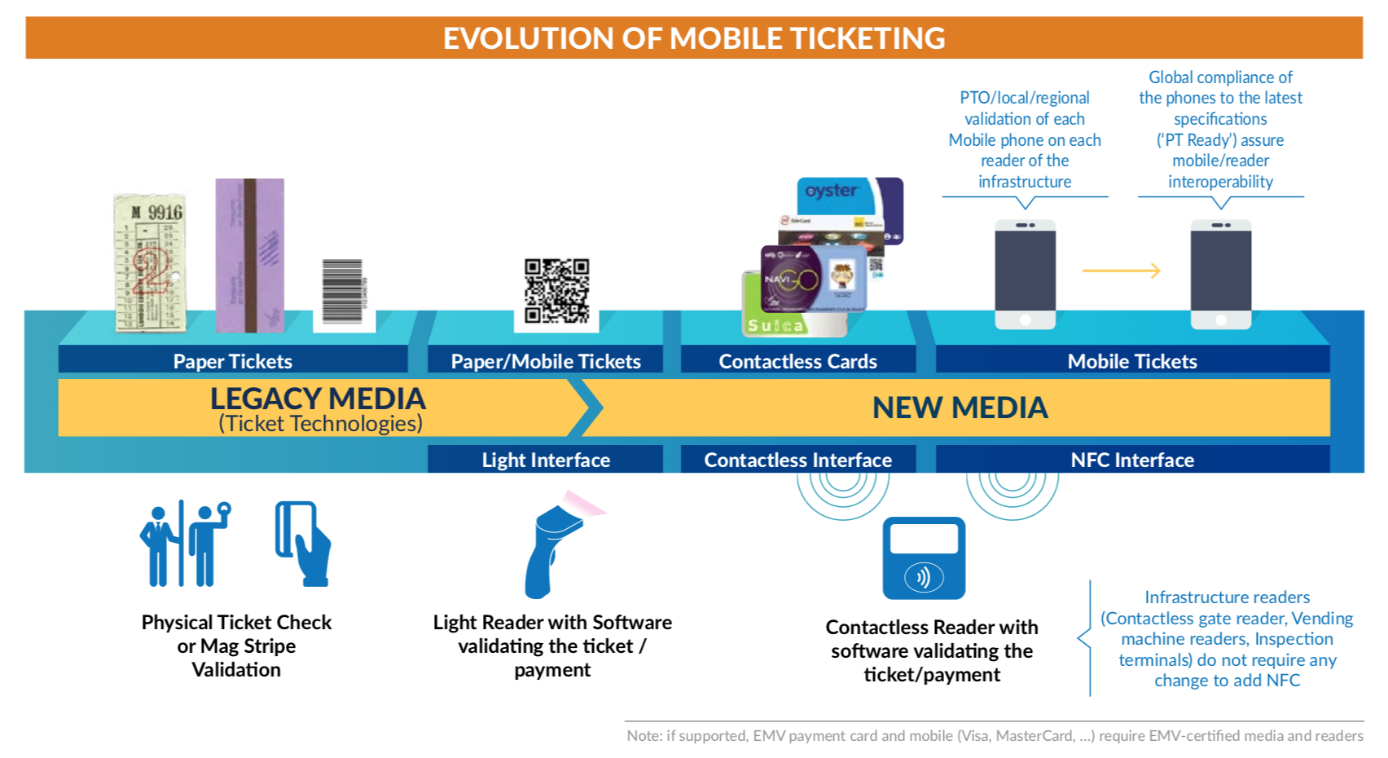
\includegraphics[width=0.9\linewidth]{image/smart_cards} \caption{Die Entwicklung des mobilen Ticketing (NFC Forum, 2016)}\label{fig:unnamed-chunk-31}
\end{figure}

Darüber hinaus befasst sich die aktuelle Forschung mit dem Thema Big Data und der Frage, wie die durch kontaktlose Chipkarten gesammelten Daten am besten ausgewertet werden können (siehe Kurauchi \& Schmöcker, 2017).

\hypertarget{aktueller-stand-der-praktischen-umsetzung-26}{%
\subsection*{Aktueller Stand der praktischen Umsetzung}\label{aktueller-stand-der-praktischen-umsetzung-26}}
\addcontentsline{toc}{subsection}{Aktueller Stand der praktischen Umsetzung}

Viele Länder, Regionen oder Städte haben Smartcard-Ticketing-Systeme im Einsatz, wie z.B. die gesamten Niederlande, die Region Helsinki, Minsk, Berlin, Auckland, Sydney und viele mehr (siehe Wikipedia-Beiträge, 2021). Die Systeme selbst sind unterschiedlich und hängen von den lokalen Fahrkarten- und Tarifsystemen ab. Während London zum Beispiel ein Zugangskontrollsystem verwendet, basiert das System in Helsinki auf Vertrauen. Außerdem kann zwischen Prepaid- (Debit) und Postpaid- (Kredit) Systemen unterschieden werden (Kurauchi \& Schmöcker, 2017).

\hypertarget{relevante-initiativen-in-uxf6sterreich-26}{%
\subsection*{Relevante Initiativen in Österreich}\label{relevante-initiativen-in-uxf6sterreich-26}}
\addcontentsline{toc}{subsection}{Relevante Initiativen in Österreich}

\begin{itemize}
\tightlist
\item
  \href{https://taikai.network/en/wiener-linien/challenges/tickethon}{taikai.network}
\item
  \href{https://www.variuscard.com/}{variuscard}
\item
  \href{https://www.austriacard.com/}{austriacard}
\end{itemize}

\hypertarget{auswirkungen-in-bezug-auf-die-ziele-fuxfcr-nachhaltige-entwicklung-sdgs-26}{%
\subsection*{Auswirkungen in Bezug auf die Ziele für nachhaltige Entwicklung (SDGs)}\label{auswirkungen-in-bezug-auf-die-ziele-fuxfcr-nachhaltige-entwicklung-sdgs-26}}
\addcontentsline{toc}{subsection}{Auswirkungen in Bezug auf die Ziele für nachhaltige Entwicklung (SDGs)}

\begin{longtable}[]{@{}ccccc@{}}
\toprule
\begin{minipage}[b]{0.17\columnwidth}\centering
Ebene der Auswirkungen\strut
\end{minipage} & \begin{minipage}[b]{0.16\columnwidth}\centering
Indikator\strut
\end{minipage} & \begin{minipage}[b]{0.17\columnwidth}\centering
Richtung der Auswirkungen\strut
\end{minipage} & \begin{minipage}[b]{0.17\columnwidth}\centering
Beschreibung des Ziels \& SDG\strut
\end{minipage} & \begin{minipage}[b]{0.17\columnwidth}\centering
Beschreibung des Ziels \& SDG\strut
\end{minipage}\tabularnewline
\midrule
\endhead
\begin{minipage}[t]{0.17\columnwidth}\centering
Individuell\strut
\end{minipage} & \begin{minipage}[t]{0.16\columnwidth}\centering
Reduzierung der persoenlichen, Reiseausgaben\strut
\end{minipage} & \begin{minipage}[t]{0.17\columnwidth}\centering
\textbf{+}\strut
\end{minipage} & \begin{minipage}[t]{0.17\columnwidth}\centering
Nachhaltige wirtschaftliche Entwicklung (\emph{8,11})\strut
\end{minipage} & \begin{minipage}[t]{0.17\columnwidth}\centering
Turner \& Wilson, 2010\strut
\end{minipage}\tabularnewline
\begin{minipage}[t]{0.17\columnwidth}\centering
Individuell\strut
\end{minipage} & \begin{minipage}[t]{0.16\columnwidth}\centering
Zugang zu digitalisiertem Verkehr\strut
\end{minipage} & \begin{minipage}[t]{0.17\columnwidth}\centering
\textbf{+}\strut
\end{minipage} & \begin{minipage}[t]{0.17\columnwidth}\centering
Innovation und Infrastruktur (\emph{9})\strut
\end{minipage} & \begin{minipage}[t]{0.17\columnwidth}\centering
Turner \& Wilson, 2010\strut
\end{minipage}\tabularnewline
\begin{minipage}[t]{0.17\columnwidth}\centering
Systemisch\strut
\end{minipage} & \begin{minipage}[t]{0.16\columnwidth}\centering
Erhoehung der Kapazitaet des oeffentlichen Verkehrs\strut
\end{minipage} & \begin{minipage}[t]{0.17\columnwidth}\centering
\textbf{+}\strut
\end{minipage} & \begin{minipage}[t]{0.17\columnwidth}\centering
Nachhaltige wirtschaftliche Entwicklung (\emph{8,11})\strut
\end{minipage} & \begin{minipage}[t]{0.17\columnwidth}\centering
Turner \& Wilson, 2010\strut
\end{minipage}\tabularnewline
\begin{minipage}[t]{0.17\columnwidth}\centering
Systemisch\strut
\end{minipage} & \begin{minipage}[t]{0.16\columnwidth}\centering
Erleichtert die Integration der Tarifsysteme mehrerer Betreiber innerhalb einer Stadt\strut
\end{minipage} & \begin{minipage}[t]{0.17\columnwidth}\centering
\textbf{+}\strut
\end{minipage} & \begin{minipage}[t]{0.17\columnwidth}\centering
Partnerschaften und Kooperationen (\emph{17})\strut
\end{minipage} & \begin{minipage}[t]{0.17\columnwidth}\centering
Kurauchi \& Schmoecker, 2017\strut
\end{minipage}\tabularnewline
\bottomrule
\end{longtable}

\hypertarget{technologie--und-gesellschaftlicher-bereitschaftsgrad-23}{%
\subsection*{Technologie- und gesellschaftlicher Bereitschaftsgrad}\label{technologie--und-gesellschaftlicher-bereitschaftsgrad-23}}
\addcontentsline{toc}{subsection}{Technologie- und gesellschaftlicher Bereitschaftsgrad}

\begin{longtable}[]{@{}cc@{}}
\toprule
Stand der Technologiebereitschaft & Gesellschaftlicher Bereitschaftsgrad\tabularnewline
\midrule
\endhead
7-9 & 7-9\tabularnewline
\bottomrule
\end{longtable}

\hypertarget{offene-fragen-24}{%
\subsection*{Offene Fragen}\label{offene-fragen-24}}
\addcontentsline{toc}{subsection}{Offene Fragen}

\begin{enumerate}
\def\labelenumi{\arabic{enumi}.}
\tightlist
\item
  Wie kann die große Menge an bereitgestellten Daten am besten genutzt werden?
\item
  Welche Vor- und Nachteile hätte eine Umsetzung in den wichtigsten Städten Österreichs?
\end{enumerate}

\hypertarget{weitere-links-22}{%
\subsection*{Weitere links}\label{weitere-links-22}}
\addcontentsline{toc}{subsection}{Weitere links}

\begin{itemize}
\tightlist
\item
  \href{https://www.itso.org.uk/}{itso}
\end{itemize}

\hypertarget{referenzen-26}{%
\subsection*{Referenzen}\label{referenzen-26}}
\addcontentsline{toc}{subsection}{Referenzen}

\begin{itemize}
\tightlist
\item
  Kurauchi, F., \& Schmöcker, J. D. (Eds.). (2017). Public transport planning with smart card data. CRC Press.
\item
  Mezghani, M. (2008). Study on electronic ticketing in public transport. European Metropolitan Transport Authorities (EMTA), 56, 38.
\item
  NFC Forum. (2016). NFC-enabled e-Ticketing in Public Transport\,: Clearing the Route to Interoperability. December. \url{https://nfc-forum.org/wp-content/uploads/2016/12/NFC_enabled_eTicketing_in_Public_Transport_White_Paper.pdf}
\item
  ÖBB. Ihr Weg zum Ticket. Available at: \url{https://www.oebb.at/de/tickets-kundenkarten/weg-zum-ticket} {[}Accessed: 13 January 2021{]}
\item
  Turner, M., \& Wilson, R. (2010). Smart and integrated ticketing in the UK: Piecing together the jigsaw. Computer Law \& Security Review, 26(2), 170-177.
\item
  Wels Linien. Tarife. Available at: \url{https://www.welslinien.at/tarife/} {[}Accessed: 13 January 2021{]}
\item
  Wiener Linien. (2021a). Der richtige Fahrschein, der passende Tarif. Available at: \url{https://www.wienerlinien.at/eportal3/ep/channelView.do/pageTypeId/66526/channelId/-46648} {[}Accessed: 13 January 2021{]}
\item
  Wiener Linien. (2021b). Digital-Wettbewerb ``Vienna Tickethon'' gestartet. Available at: \url{https://www.wienerlinien.at/eportal3/ep/contentView.do/pageTypeId/66526/programId/74577/contentTypeId/1001/channelId/-47186/contentId/5002360\#}:\textasciitilde:text=Im\%20Rahmen\%20eines\%20internationalen\%20Hackathon,Wettbewerb\%20l\%C3\%A4uft\%20bis\%20Anfang\%20M\%C3\%A4rz {[}Accessed: 13 January 2021{]}
\item
  Wikipedia contributors. (2021, January 8). List of smart cards. In Wikipedia, The Free Encyclopedia. Available at: \url{https://en.wikipedia.org/w/index.php?title=List_of_smart_cards\&oldid=999040130} {[}Accessed: 13 January 2021{]}
\end{itemize}

\hypertarget{special_needs}{%
\section{Informationen und Unterstützung für Menschen mit besonderen Bedürfnissen}\label{special_needs}}

\hypertarget{synonyme-22}{%
\subsection*{Synonyme}\label{synonyme-22}}
\addcontentsline{toc}{subsection}{Synonyme}

\emph{Assistierende Technologie, \href{http://changemobility.at/wiki/index.php?title=Barrieren_\%26_Disparit\%C3\%A4ten}{Barrieren \& Disparitäten}}

\hypertarget{definition-27}{%
\subsection*{Definition}\label{definition-27}}
\addcontentsline{toc}{subsection}{Definition}

Vehmas (2010: 92) definiert, dass ein besonderer Bedarf \emph{``\ldots bedeutet, dass eine Person Merkmale aufweist, bei denen es unwahrscheinlich oder zumindest ungewiss ist, ob sie das Ziel, das den betreffenden Bedarf definiert, ohne besondere Anleitung, ohne ungewöhnliche Verfahren erreichen würde.''} Besondere Bedürfnisse können also eine altersbedingte Mobilitätseinschränkung oder jede Art von Behinderung bedeuten.
Darüber hinaus \emph{``bezieht sich unterstützende Technologie auf jedes System, jede Dienstleistung, jedes Gerät oder jede Vorrichtung, die verwendet werden können, um Menschen mit Behinderungen in ihrem täglichen Leben zu helfen, indem sie einige Barrieren für Aktivitäten beseitigen.''} (Low et al., 2020).
Da die Arten von Behinderungen vielfältig sind und die spezifischen Bedürfnisse ebenso, argumentieren Low et al.~(2020), dass spezifischere Maßnahmen ergriffen werden sollten, um die besonderen Bedürfnisse spezifischer Behinderungen zu erfüllen, anstatt die verfügbaren Hilfsmittel zu verallgemeinern. Die Anforderungen an Verkehrssysteme für Menschen mit besonderen Bedürfnissen können unterteilt werden in \emph{(1)} Sehbehinderung, \emph{(2)} Hörbehinderung, \emph{(3)} Mobilitätsbehinderung und \emph{(4)} geistige Behinderung. Während für einige Menschen mit besonderen Bedürfnissen möglicherweise nur eines der drei Kriterien zutrifft, sind ältere Menschen möglicherweise auf mehr als eines oder sogar auf alle angewiesen.

Low et al.~(2020) argumentieren, dass vor allem Menschen mit Sehbehinderungen (VIP - visual impairment) auf öffentliche Verkehrsmittel angewiesen sind, da sie selbst keine Fahrzeuge fahren können, was zu einer Einschränkung der Bewegungsfreiheit führt. Das Gleiche gilt für viele Menschen mit eingeschränkter Mobilität, die von der aktiven Teilnahme am motorisierten Individualverkehr ausgeschlossen sind. Der eingeschränkte Zugang zu Reiseinformationen ist für Menschen mit besonderen Bedürfnissen oft ein Hindernis für das unabhängige Reisen und andere tägliche Aktivitäten. Bei der Nutzung öffentlicher Verkehrsmittel wird die Wahl der Route von der Zuverlässigkeit und Verfügbarkeit von Informationen sowie von der Bequemlichkeit und dem Komfort beeinflusst. Die einfache Beschaffung dieser Informationen vor einer Reise kann jedoch für VIPs oft ein Problem darstellen, da viele Informationen gedruckt werden. Der aktuelle Trend zu Online-Materialien ist jedoch hilfreich. Aufgrund ihrer körperlichen und geistigen Verfassung benötigen vor allem ältere oder behinderte Menschen möglicherweise zusätzliche Informationen. Viele ältere Menschen können beispielsweise nicht lange stehen, reagieren empfindlich auf Wetterbedingungen, können Dinge nicht schnell erledigen oder keine langen Strecken zu Fuß zurücklegen (Hounsell et al., 2016). Ein Mangel an brauchbaren Informationen kann das Gesamterlebnis negativ beeinflussen und sogar eine Reise verhindern.

Darüber hinaus argumentieren Low et al.~(2020), dass das Busfahren für VIPs mehrere Herausforderungen mit sich bringt, wie z. B. das Auffinden des richtigen Busses, was besonders problematisch ist, wenn sich mehrere Bushaltestellen an derselben Haltestelle befinden. Die Mischung der eingesetzten Flotten macht es für VIPs schwierig, die Merkmale eines Busses zu erkennen. Außerdem ist es für VIPs oft schwierig, den Einstiegspunkt für Busse zu finden. Bei Zügen kann die Lücke zwischen dem Zug und dem Bahnsteig ein Hindernis darstellen. Ein wichtiger Bestandteil der öffentlichen Verkehrsmittel sind Audio-Durchsagen, die als Informationsquelle für VIPs dienen. Wenn diese Systeme ausfallen, wird die Reise als besonders stressig empfunden.

Zur Überwindung von Barrieren beim Fahrkartenkauf kann die Einführung von kontaktlosen Kartensystemen (siehe Abschnitt \protect\hyperlink{contactless_cards}{Kontaktlose ÖPNV-Karten}) oder Freikarten für Menschen mit Behinderungen beitragen (Low et al., 2020).

\hypertarget{wichtige-interessensgruppen-27}{%
\subsection*{Wichtige Interessensgruppen}\label{wichtige-interessensgruppen-27}}
\addcontentsline{toc}{subsection}{Wichtige Interessensgruppen}

\begin{itemize}
\tightlist
\item
  \textbf{Betroffene}: Menschen mit besonderen Bedürfnissen, ältere Menschen, Pfleger:innen
\item
  \textbf{Verantwortliche}: Verkehrsdienstleister und Betreiber öffentlicher Verkehrsmittel, MaaS-Betreiber und -Integratoren, IT-Systemanbieter, Stadtverwaltungen, lokale, regionale und nationale Behörden, Verbände des öffentlichen Nahverkehrs, Zulieferer der Branche, Blindenverband, Behindertenverband
\end{itemize}

\hypertarget{aktueller-stand-der-wissenschaft-und-forschung-27}{%
\subsection*{Aktueller Stand der Wissenschaft und Forschung}\label{aktueller-stand-der-wissenschaft-und-forschung-27}}
\addcontentsline{toc}{subsection}{Aktueller Stand der Wissenschaft und Forschung}

Die Studie von Low et al.~(2020) spiegelt unter anderem den Wunsch der VIPs wider, bei der Planung ihrer Reisen unabhängig zu sein, indem sie Online-Ressourcen nutzen, anstatt Hilfe von anderen zu suchen. Dies zeigt, wie wichtig es ist, geeignete Online-Tools für VIPs zu haben. Die Befragten gaben an, dass sie viele verschiedene Quellen und Apps nutzen müssen, um eine einzige Reise zu planen, was wiederum eine Menge Stress verursacht und die Bereitschaft zur Nutzung öffentlicher Verkehrsmittel verringert. Darüber hinaus wurde festgestellt, dass die VIPs keinen Zugang zu aktuellen Maßnahmen und Informationen über verfügbare Unterstützung haben. Außerdem wurde darauf hingewiesen, dass eine ähnliche Innenraumgestaltung der Busse für VIP äußerst hilfreich wäre und die Sicherheit erhöhen würde.

Goldberg et al.~(2018) untersuchten die Bedürfnisse von VIPs in Bezug auf Orientierung, Navigation und Mobilität. Auf der Grundlage ihrer Ergebnisse schlagen sie \emph{``ein integriertes cyber-physisches System (CPS) mit `Agenten' und `Smart Environments' vor, um die ONM-Bedürfnisse von VIPs in städtischen Umgebungen zu adressieren.''} Fusco \& Coughlan (2020) beschreiben \emph{``einen Computer-Vision-Ansatz zur Lokalisierung in Innenräumen, der als Echtzeit-App auf einem herkömmlichen Smartphone läuft und in Zukunft eine vollwertige Wayfinding-App unterstützen soll, die auch Abbiegehinweise enthält.''} Ein Vorteil dieses Ansatzes ist, dass keine neue Infrastruktur benötigt wird, sondern lediglich ein funktionierendes Smartphone mit eingebauter Kamera.

Hounsell et al.~(2016) untersuchten die Informationsbedürfnisse älterer Menschen, die insbesondere öffentliche Verkehrsmittel nutzen. Sie fanden unter anderem heraus, dass ältere Menschen \emph{``möglicherweise nur größere Schriftanzeigen und Primärdaten benötigen, während mobilitätseingeschränkte Menschen Informationen über Gehentfernungen und das Vorhandensein von Steigungen, Stufen, Sitzen usw. benötigen.''} Bei der Überprüfung internationaler Beispiele für die Umsetzung offener Daten fanden sie Beispiele für Behörden, die den Markt durch die Durchführung von Wettbewerben zur Entwicklung von Apps für bestimmte Zielgruppen wie ältere oder behinderte Menschen initiierten.

\hypertarget{aktueller-stand-der-praktischen-umsetzung-27}{%
\subsection*{Aktueller Stand der praktischen Umsetzung}\label{aktueller-stand-der-praktischen-umsetzung-27}}
\addcontentsline{toc}{subsection}{Aktueller Stand der praktischen Umsetzung}

Eines der üblichen Hilfsmittel für VIP sind Mobilitätshilfen, insbesondere ein Langstock oder ein Blindenhund. GPS wird als unterstützende Technologie für VIP zu Orientierungszwecken und als Navigationshilfe eingesetzt. Es kann auch in andere Geräte integriert werden, um VIP bei der Orientierung zu helfen, z. B. in ein GPS-basiertes Sprachalarmsystem, das VIP vor Hindernissen in der Nähe warnt (Low et al., 2020). \emph{BlindSquare} ist eine der weltweit beliebtesten GPS-Apps für blinde und sehbehinderte Menschen. Sie beschreibt die Umgebung, warnt vor Straßenkreuzungen und wichtigen Punkten, während man sich fortbewegt. In Verbindung mit externen kostenlosen Navigations-Apps bietet \emph{BlindSquare} fast alle Informationen, die blinde und sehbehinderte Menschen benötigen, um unabhängig im Straßenverkehr zu sein. BlindSquare ermittelt den Standort mithilfe der GPS-Funktionen des Smartphones und ruft Informationen über die Umgebung auf Foursquare und Open Street Map ab. Dank seiner einzigartigen Algorithmen ermittelt es die wichtigsten Informationen und gibt sie mit einer künstlichen Stimme deutlich wieder (BlindSquare., n.d.). Eine ähnliche App ist \emph{Seeing Assistant Move}, die auf Google Maps basiert und ebenfalls offline und mit Sprachsteuerung funktioniert (Transition Technologies S.A., n.d.). Bei der Nutzung öffentlicher Verkehrsmittel spielen akustische Ansagen eine entscheidende Rolle, um VIPs beim Aussteigen aus dem Fahrzeug zu unterstützen (Low et al., 2020).

Induktionshörsysteme oder Induktionshörschleifen werden eingesetzt, um Menschen mit Hörproblemen mit auditiven Informationen zu versorgen. Das Prinzip basiert auf speziellen Kabeln, der sogenannten Induktionsschleife, die von einem Induktionsverstärker betrieben wird, der die vom Mikrofon kommenden Signale umwandelt und als Strom in die Schleife einspeist. Dieser Strom wiederum erzeugt in der Spule im Raum ein schwaches Magnetfeld, das im Rhythmus der Sprache pulsiert. Dieses schwache Magnetfeld wird von der T-Spule des Hörgeräts, ähnlich einer Antenne, aufgefangen und in hörbare Schallschwingungen zurückverwandelt. Es werden fast keine Hintergrundgeräusche übertragen und die gewünschten Informationen können so ohne Störungen, fast in HIFI-Qualität, gehört werden (Sturma, 2011).

Um die Zugänglichkeit für Menschen mit eingeschränkter Mobilität in Bussen zu gewährleisten, setzen immer mehr Städte auf den Einsatz von Niederflurfahrzeugen, die bei Bedarf hydraulisch weiter abgesenkt werden können. Die niedrige Einstiegshöhe erleichtert das Ein- und Aussteigen, insbesondere für ältere Menschen und Fahrgäste mit Kinderwagen oder Rollstuhlfahrer, erheblich. Auch die Ausstattung der Stadtbahn wird ständig verbessert. Moderne Fahrzeuge verfügen über mehr Platz für Fahrgäste mit Rollstühlen oder Kinderwagen und eine ausfahrbare Rampe zur Überbrückung des ohnehin minimierten Spalts zwischen Bahnsteigkante und Fahrzeug (Wiener Linien, n.d.). Wie in Wien können z.B. Echtzeitanzeigen an Bahnhöfen mit einem Rollstuhlsymbol anzeigen, ob die zu erwartenden ÖPNV-Fahrzeuge barrierefrei sind.

Schließlich wurden beispielsweise in Bussen in Singapur Annehmlichkeiten für schwangere, ältere und junge Fahrgäste in Form von ausgewiesenen Vorrangsitzen, niedrigen Böden entlang des gesamten Busses und niedrigen Stufen am Ein- und Ausstieg eingeführt, um Personen mit eingeschränkter Mobilität einen schnellen Einstieg in den Bus zu ermöglichen und ihnen die Bewegung im Bus zu erleichtern (Smrt.com.sg, 2021).

\hypertarget{relevante-initiativen-in-uxf6sterreich-27}{%
\subsection*{Relevante Initiativen in Österreich}\label{relevante-initiativen-in-uxf6sterreich-27}}
\addcontentsline{toc}{subsection}{Relevante Initiativen in Österreich}

\begin{itemize}
\tightlist
\item
  \href{https://www.oebb.at/de/reiseplanung-services/barrierefrei-reisen}{oebb.at}
\item
  \href{https://www.wienerlinien.at/web/wiener-linien/neue-bim-und-bus-haltestellen-f\%C3\%BCr-wien}{wienerlinien.at}
\item
  \href{https://www.induktionsschleife.at/}{induktionsschleife.at}
\end{itemize}

\hypertarget{auswirkungen-in-bezug-auf-die-ziele-fuxfcr-nachhaltige-entwicklung-sdgs-27}{%
\subsection*{Auswirkungen in Bezug auf die Ziele für nachhaltige Entwicklung (SDGs)}\label{auswirkungen-in-bezug-auf-die-ziele-fuxfcr-nachhaltige-entwicklung-sdgs-27}}
\addcontentsline{toc}{subsection}{Auswirkungen in Bezug auf die Ziele für nachhaltige Entwicklung (SDGs)}

\begin{longtable}[]{@{}ccccc@{}}
\toprule
\begin{minipage}[b]{0.17\columnwidth}\centering
Ebene der Auswirkungen\strut
\end{minipage} & \begin{minipage}[b]{0.16\columnwidth}\centering
Indikator\strut
\end{minipage} & \begin{minipage}[b]{0.17\columnwidth}\centering
Richtung der Auswirkungen\strut
\end{minipage} & \begin{minipage}[b]{0.17\columnwidth}\centering
Beschreibung des Ziels \& SDG\strut
\end{minipage} & \begin{minipage}[b]{0.17\columnwidth}\centering
Beschreibung des Ziels \& SDG\strut
\end{minipage}\tabularnewline
\midrule
\endhead
\begin{minipage}[t]{0.17\columnwidth}\centering
Individuell\strut
\end{minipage} & \begin{minipage}[t]{0.16\columnwidth}\centering
Sicherer Zugang zu oeffentlichen Verkehrsmitteln fuer Menschen mit Behinderungen\strut
\end{minipage} & \begin{minipage}[t]{0.17\columnwidth}\centering
\textbf{+}\strut
\end{minipage} & \begin{minipage}[t]{0.17\columnwidth}\centering
Gesundheit und Wohlbefinden (\emph{3})\strut
\end{minipage} & \begin{minipage}[t]{0.17\columnwidth}\centering
Low et al.~(2020)\strut
\end{minipage}\tabularnewline
\begin{minipage}[t]{0.17\columnwidth}\centering
Individuell\strut
\end{minipage} & \begin{minipage}[t]{0.16\columnwidth}\centering
Gleiche Bewegungsfreiheit fuer Menschen mit Behinderungen\strut
\end{minipage} & \begin{minipage}[t]{0.17\columnwidth}\centering
\textbf{+}\strut
\end{minipage} & \begin{minipage}[t]{0.17\columnwidth}\centering
Gleichheit (\emph{5,10})\strut
\end{minipage} & \begin{minipage}[t]{0.17\columnwidth}\centering
Low et al.~(2020)\strut
\end{minipage}\tabularnewline
\begin{minipage}[t]{0.17\columnwidth}\centering
Individuell\strut
\end{minipage} & \begin{minipage}[t]{0.16\columnwidth}\centering
Verbesserter Zugang zu oeffentlichen Verkehrsmitteln\strut
\end{minipage} & \begin{minipage}[t]{0.17\columnwidth}\centering
\textbf{+}\strut
\end{minipage} & \begin{minipage}[t]{0.17\columnwidth}\centering
Oekologische Nachhaltigkeit (\emph{7,12-13,15})\strut
\end{minipage} & \begin{minipage}[t]{0.17\columnwidth}\centering
Low et al.~(2020)\strut
\end{minipage}\tabularnewline
\begin{minipage}[t]{0.17\columnwidth}\centering
Systemisch\strut
\end{minipage} & \begin{minipage}[t]{0.16\columnwidth}\centering
Zunahme innovativer, fuer Zielgruppen entwickelter Apps; Nutzung offener Daten\strut
\end{minipage} & \begin{minipage}[t]{0.17\columnwidth}\centering
\textbf{+}\strut
\end{minipage} & \begin{minipage}[t]{0.17\columnwidth}\centering
Innovation und Infrastruktur (\emph{9})\strut
\end{minipage} & \begin{minipage}[t]{0.17\columnwidth}\centering
Hounsell et al.~(2016)\strut
\end{minipage}\tabularnewline
\bottomrule
\end{longtable}

\hypertarget{technologie--und-gesellschaftlicher-bereitschaftsgrad-24}{%
\subsection*{Technologie- und gesellschaftlicher Bereitschaftsgrad}\label{technologie--und-gesellschaftlicher-bereitschaftsgrad-24}}
\addcontentsline{toc}{subsection}{Technologie- und gesellschaftlicher Bereitschaftsgrad}

\begin{longtable}[]{@{}cc@{}}
\toprule
Stand der Technologiebereitschaft & Gesellschaftlicher Bereitschaftsgrad\tabularnewline
\midrule
\endhead
3-7 & 3-7\tabularnewline
\bottomrule
\end{longtable}

\hypertarget{offene-fragen-25}{%
\subsection*{Offene Fragen}\label{offene-fragen-25}}
\addcontentsline{toc}{subsection}{Offene Fragen}

\begin{enumerate}
\def\labelenumi{\arabic{enumi}.}
\tightlist
\item
  Wie könnten Echtzeitinformationen für sehbehinderte Menschen besser zugänglich gemacht werden?
\item
  Wie könnten Audio-Durchsagen verbessert werden?
\item
  Wie kann die Unterstützung durch das Personal verbessert werden?
\item
  Wie könnten intelligente Technologien für ältere Menschen zugänglicher werden
\end{enumerate}

\hypertarget{weitere-links-23}{%
\subsection*{Weitere links}\label{weitere-links-23}}
\addcontentsline{toc}{subsection}{Weitere links}

\begin{itemize}
\tightlist
\item
  \href{https://www.blindsquare.com/de/about/}{blindsquare.com}
\item
  \href{http://seeingassistant.tt.com.pl/move/}{seeingassistant.tt.com.pl}
\item
  \href{https://www.induktionsschleife.at/anwendungen/}{induktionsschleife.at}
\item
  \href{https://www.oebb.at/de/reiseplanung-services/barrierefrei-reisen}{oebb.at}
\item
  \href{https://www.wienerlinien.at/eportal3/ep/contentView.do?pageTypeId=66526\&channelId=-47186\&programId=74577\&contentId=5002349\&contentTypeId=1001}{wienerlinien.at}
\item
  \href{https://www.oesb-dachverband.at/}{oesb-dachverband.at}
\item
  \href{https://www.blindenverband.at/}{blindenverband.at}
\end{itemize}

\hypertarget{referenzen-27}{%
\subsection*{Referenzen}\label{referenzen-27}}
\addcontentsline{toc}{subsection}{Referenzen}

\begin{itemize}
\tightlist
\item
  BlindSquare. (n.d.). What is BlindSquare? Available at: March 4, 2021, from \url{https://www.blindsquare.com/about/} {[}Accessed: 4 March 2021{]}
\item
  Fusco, G., \& Coughlan, J. M. (2020, April). Indoor localization for visually impaired travelers using computer vision on a smartphone. In Proceedings of the 17th International Web for All Conference (pp.~1-11).
\item
  Goldberg, M., Zhu, Z., \& Zhang, Z. (2018). How do we aid visually impaired people safely manage unfamiliar environments?.
\item
  Hounsell, N. B., Shrestha, B. P., McDonald, M., \& Wong, A. (2016). Open data and the needs of older people for public transport information. Transportation research procedia, 14, 4334-4343.
\item
  Low, W. Y., Cao, M., De Vos, J., \& Hickman, R. (2020). The journey experience of visually impaired people on public transport in London. Transport Policy, 97, 137-148.
\item
  Smrt.com.sg. (2021). Accessibility. Smrt.com.sg. Available at: \url{https://www.smrt.com.sg/Journey-with-Us/SMRT-Buses/Accessibility} {[}Accessed: 12 March 2021{]}.
\item
  Sturma, A. (2011). Höranlagen. \url{https://www.oessh.or.at/hoerspuren/hoeranlagen}
\item
  Transition Technologies S.A. (n.d.). Seeing Assistant Move - Features. Available at: \url{http://seeingassistant.tt.com.pl/move/} {[}Accessed: 4 March 2021{]}
\item
  Vehmas, S. (2010). Special needs: a philosophical analysis. International journal of inclusive education, 14(1), 87-96.
\item
  Wiener Linien. (n.d.). Barrierefreiheit bei den Wiener Linien - Wiener Linien. Available at: \url{https://www.wienerlinien.at/web/wiener-linien/barrierefreiheit} {[}Accessed: 16 March 2021{]}
\end{itemize}

\hypertarget{mobility_hubs}{%
\section{Mobilitätszentren - Mobility hubs}\label{mobility_hubs}}

\hypertarget{synonyme-23}{%
\subsection*{Synonyme}\label{synonyme-23}}
\addcontentsline{toc}{subsection}{Synonyme}

\emph{Mobilitätsstation oder -punkt, Mobihub, (öffentlicher) Ride Point, Smart Station, Sharing Zone, Verkehrszentrum, ÖPNV, Verkehrsknotenpunkt, Ride Port, Share Point, intermodale Knotenpunkte, \href{http://changemobility.at/wiki/index.php?title=Multimodale_Mobilit\%C3\%A4t}{Multimodale Mobilität}}

\hypertarget{definition-28}{%
\subsection*{Definition}\label{definition-28}}
\addcontentsline{toc}{subsection}{Definition}

Es gibt viele verschiedene Definitionen von Mobilitätsknotenpunkten. Im Allgemeinen sind Mobilitätsknotenpunkte Orte, an denen man das Verkehrsmittel wechseln kann. Sie können aber auch viel mehr als das sein und sind für das Funktionieren von Mobility as a Service unerlässlich (siehe \protect\hyperlink{maas}{Abschnitt Mobilität als Dienstleistung}). Von Mobilitätsknotenpunkten wird erwartet, dass sie einen bequemen und sicheren Wechsel des Verkehrsträgers ermöglichen, aber sie könnten auch Versorgungslücken schließen, die Erfahrungen der Reisenden verbessern und die Lebensqualität in einem bestimmten Gebiet erhöhen (Clemens, 2020). Flughäfen, Bahnhöfe und U-Bahn-Stationen umfassen in der Regel Parkplätze und Autovermietungen, Bushaltestellen und Taxistände sowie Restaurants, Geschäfte, Hotels oder sogar Konferenzzentren, die von der Erreichbarkeit durch Handel und Waren profitieren. Sie stellen sogenannte \emph{``natürlich''} gewachsene Megahubs dar (Clemens, 2020). Darüber hinaus planen und realisieren Kommunen weltweit systematisch weitere Mobilitätsknotenpunkte unterschiedlicher Größe - von einer kleinen Bushaltestelle mit angeschlossener Bike-Sharing-Station bis hin zu einem Mega-Hub wie oben beschrieben. Sie sollen die intermodale Mobilität verbessern und sozioökonomische Vorteile bringen (Clemens, 2020). Spezifische Namen und ein starkes visuelles Branding sollen den Fahrgästen helfen, sie schnell zu erkennen.

Mobility-as-a-Service- oder Mobility-on-Demand-Konzepte sollen es ermöglichen, kein eigenes Auto zu besitzen und trotzdem mobil zu sein. Mobilitätsknotenpunkte sollen eine möglichst große Variation an Verkehrsmitteln für einzelne Wegeketten anbieten und so dafür sorgen, dass nicht alle Autofahrten eins zu eins durch Carsharing-Fahrten ersetzt werden, sondern dass die Verkehrswege möglichst nachhaltig zurückgelegt werden (Clemens, 2020). Da jedes zusätzliche Umsteigen während einer Reise eine Barriere darstellt und die Menschen dazu verleitet, stattdessen den motorisierten Individualverkehr zu nutzen, ist es das Ziel von Mobilitätsdrehscheiben, diese Umstiege mit einem Nutzen zu versehen und einen reibungslosen Ablauf zu gewährleisten. So können die Menschen beispielsweise arbeiten oder sich entspannen, ein Paket abholen, Freunde treffen oder notwendige Einkäufe auf dem Heimweg erledigen (Clemens, 2020). Mobilitätsknotenpunkte könnten auch mit Quartierslogistikknotenpunkten kombiniert werden (siehe \protect\hyperlink{urban_delivery}{Stadtlieferungen}) (Herrmann, n.d.).

\hypertarget{wichtige-interessensgruppen-28}{%
\subsection*{Wichtige Interessensgruppen}\label{wichtige-interessensgruppen-28}}
\addcontentsline{toc}{subsection}{Wichtige Interessensgruppen}

\begin{itemize}
\tightlist
\item
  \textbf{Betroffene}: Alle Arten von Passagieren
\item
  \textbf{Verantwortliche}: Stadtverwaltung, ÖPNV-Betreiber, Mobilitätsdienstleister, Fördermittelgeber, Bezirksämter, Privatunternehmen
\end{itemize}

\hypertarget{aktueller-stand-der-wissenschaft-und-forschung-28}{%
\subsection*{Aktueller Stand der Wissenschaft und Forschung}\label{aktueller-stand-der-wissenschaft-und-forschung-28}}
\addcontentsline{toc}{subsection}{Aktueller Stand der Wissenschaft und Forschung}

Bell (2019) hat die Nutzeranforderungen von Mobilitätsknotenpunkten analysiert. Er argumentiert, dass sich Mobilitätsknotenpunkte oder intermodale Knotenpunkte je nach dem Gebiet, in dem sie eingerichtet werden, unterscheiden (z. B. in ländlichen oder städtischen Gebieten) und dass Erfolg und Nachhaltigkeit stark von der jeweiligen Gestaltung abhängen. Ein Überblick über seine allgemeine Schlussfolgerung ist in Abbildung 7.2 dargestellt.

\begin{figure}
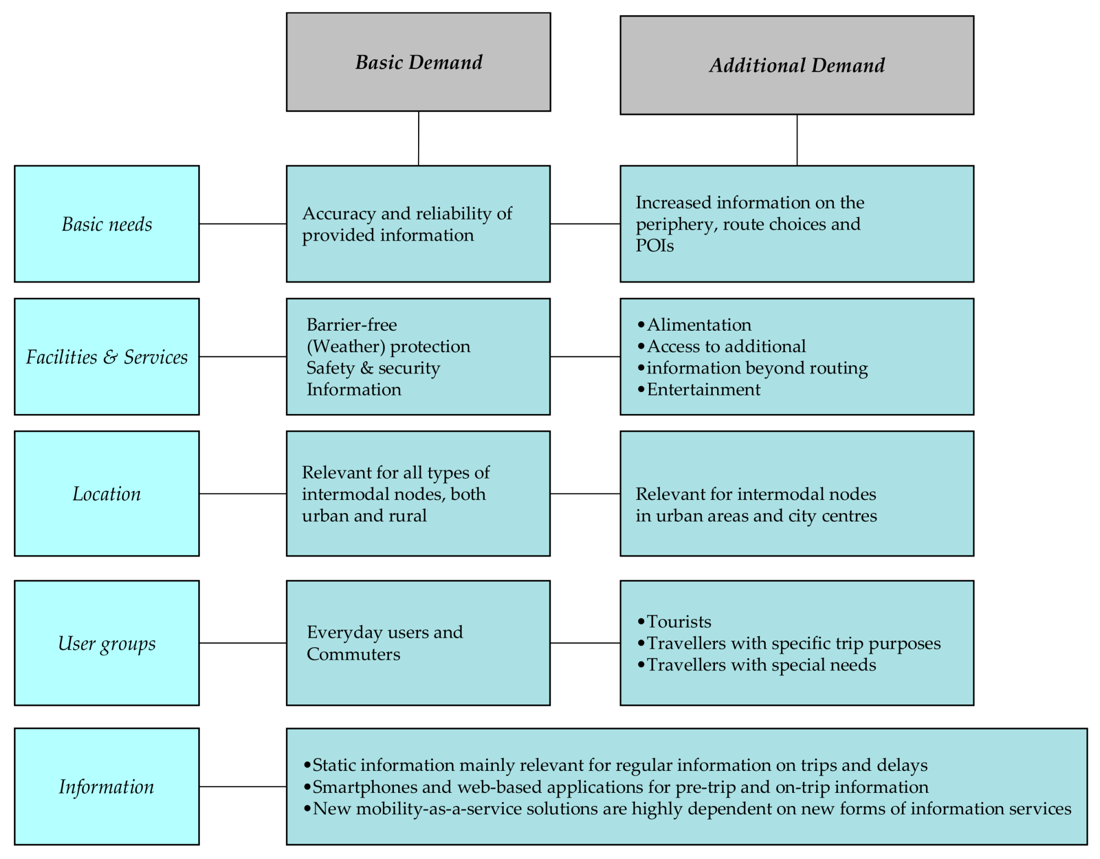
\includegraphics[width=0.65\linewidth]{image/mobility_hubs} \caption{: Nutzeranforderungen an Haltestellen des oeffentlichen Verkehrs (Bell, 2019)}\label{fig:unnamed-chunk-32}
\end{figure}

Basierend auf Untersuchungen in amerikanischen Städten argumentiert Hochmair (2015), dass es empfehlenswert ist, eine verbesserte Fahrradinfrastruktur, wie z.B. Bike-Sharing-Stationen, innerhalb eines Radius von 1 Meile für reine Bushaltestellen und innerhalb von 2 Meilen für Bahnstationen zu gewährleisten.

Tran \& Draeger (2021) haben einen neuen Bewertungsrahmen und -algorithmus vorgestellt, um die Auswirkungen von Knotenpunkten auf Nachhaltigkeit und Gerechtigkeit in Städten zu ermitteln und zu bewerten. Investitionsstrategien für Knotenpunkte werden auf der Grundlage von \emph{(1)} dem aktuellen Verkehrsmittel-Split, \emph{(2)} einer hohen Transitkapazität und \emph{(3)} multimodalen Dienstleistungen bewertet. Unter dem Gesichtspunkt der Chancengleichheit schließen Strategien für hohe Transitkapazitäten und multimodale Knotenpunkte mehr einkommensschwache Gebiete ein als der derzeitige Modussplit, der in erster Linie Gebiete mit mittlerem Einkommen umfasst. Die Ergebnisse der Studie zeigen, wie Kommunen strategisch in den öffentlichen Nahverkehr und multimodale Optionen investieren können, um die Frequenz, Qualität und Gesamtmobilität für Haushalte mit niedrigem und mittlerem Einkommen zu erhöhen und den Zugang zu wichtigen Einrichtungen für schwächere Bürger:innen zu verbessern. Die Gemeinden können den Bewertungsrahmen nutzen, um alternative Investitionsszenarien für den Verkehr zu untersuchen. Dies sollte es ermöglichen, städtische Knotenpunkte räumlich so zu platzieren, dass sie die künftige Verkehrsnachfrage decken, die Inanspruchnahme multimodaler Dienste erhöhen und den gleichberechtigten Zugang für alle Bürger:innen verbessern.

Franken (2021) untersuchte das Potenzial von Mobilitätsknotenpunkten zur Verringerung der Autonutzung und des Autobesitzes und wie diese von den Merkmalen der Autobesitzer:innen, den Merkmalen der Fahrt und den Merkmalen des Wohnumfelds der Autobesitzer:innen beeinflusst werden. Seine Ergebnisse zeigten, dass die Betriebskosten von gemeinsam genutzten Mobilitätsdiensten und die Fußwege zu Mobilitätszentren wichtige Determinanten für die Nutzung von gemeinsam genutzten Mobilitätsdiensten sind, wobei die Betriebskosten für gemeinsam genutzte E-Autos stärker ins Gewicht fallen als für gemeinsam genutzte E-Mopeds und E-Bikes. Außerdem stellte er fest, dass die Dichte von Mobilitätszentren in einem Wohngebiet einen starken Einfluss auf die Verringerung der Autonutzung und des Autobesitzes hat. Dies deckt sich mit der Tatsache, dass die Auswirkungen von Mobilitätszentren auf die Autonutzung und den Autobesitz im Stadtzentrum am höchsten waren, gefolgt von einem Vorstadtgebiet und am niedrigsten in einem ländlichen Gebiet.

Die MA 18 - Stadtentwicklung und Stadtplanung und die MA 21 - Bezirksplanung und Flächennutzung der Stadt Wien haben 2018 einen Leitfaden für die Umsetzung von Mobilitätsstationen in Stadtentwicklungsgebieten veröffentlicht (Stadt Wien - Stadtentwicklung und Stadtplanung (MA 18) \& Stadtteilplanung und Flächennutzung (MA 21), 2018). Im Auftrag des Bundesministeriums für Umwelt, Naturschutz und Reaktorsicherheit (BMU) veröffentlichte auch das Deutsche Institut für Urbanistik 2019 einen Bericht über die Erkenntnisse und Erfahrungen zu Mobilitätsstationen in der kommunalen Praxis (Stein \& Bauer, 2019).

\hypertarget{aktueller-stand-der-praktischen-umsetzung-28}{%
\subsection*{Aktueller Stand der praktischen Umsetzung}\label{aktueller-stand-der-praktischen-umsetzung-28}}
\addcontentsline{toc}{subsection}{Aktueller Stand der praktischen Umsetzung}

Um sowohl die Gesundheit als auch die Lebensqualität der Bürger:innen zu fördern und gleichzeitig die Nachhaltigkeit und Zugänglichkeit des Verkehrs in den Städten zu verbessern, haben sich sechs Partnerstädte aus fünf verschiedenen Ländern dazu verpflichtet, sogenannte e-Mobility Hubs, kurz eHUBS, einzurichten. eHUBS sind Standorte auf der Straße, an denen E-Bikes, E-Lastenräder, E-Scooter und/oder E-Autos zusammengeführt werden und die den Nutzer:innen eine breite Palette an Möglichkeiten bieten, die sie in verschiedenen Situationen ausprobieren und nutzen können. Diese speziellen Standorte auf der Straße, an denen die Bürger:innen aus einer Vielzahl nachhaltiger elektrischer Transportmöglichkeiten für die gemeinsame Nutzung wählen können, sollen eine echte Alternative zur Nutzung des privaten Autos bieten, indem sie Möglichkeiten zur Steigerung der gemeinsamen und elektrischen Mobilität auf eine wirklich innovative Weise bieten. Die Hubs können in Bezug auf Größe (minimalistisch, leicht, mittel, groß), Standort und Art der Dienstleistung variieren. Sie können klein sein und in Wohngebieten liegen, mit nur einem oder zwei Parkplätzen, oder größer und in der Nähe von Bahnhöfen und wichtigen Knotenpunkten des öffentlichen Nahverkehrs positioniert sein, aber letztlich ist der Schlüssel, dass sie immer dort sein sollten, wo Angebot und Nachfrage aufeinander treffen. Die gewonnenen Erkenntnisse und Erfahrungen werden dann anderen Städten und Regionen helfen, sich anzunähern und konsequent gegen Luftverschmutzung, Staus und CO\textsubscript{2}-Emissionen vorzugehen und einen wachsenden Markt für kommerzielle E-Mobilitätsanbieter zu schaffen (Interreg North-West Europe (NWE), 2019).

In Wien gibt es bereits 8 sogenannte \emph{``WienMobil-Stationen''} der Wiener Linien, die den Zugang zum öffentlichen Verkehr mit verschiedenen Dienstleistungen und Sharing-Angeboten kombinieren. Diese variieren je nach Station, können aber Bike-Sharing, Scooter-Sharing, Moped-Sharing, Car-Sharing, Fahrradservicestation, Taxi, E-Ladestation, Fahrradboxen und Lastenräder umfassen (Wiener Linien, 2021).

Darüber hinaus wurden in den Städten Graz und Linz sowie in der steirischen Zentralregion Mobilitätsknotenpunkte namens ``tim'' eingerichtet. Sie kombinieren Haltestellen des öffentlichen Verkehrs mit (E-)Carsharing, Anrufsammeltaxis, Fahrradabstellanlagen und mietbaren Lastenrädern (siehe \href{https://www.tim-oesterreich.at}{tim-oesterreich}).

Auch in den Niederlanden gibt es bereits mehrere Mobilitätsknotenpunkte unterschiedlicher Art. Ein Beispiel ist der Knotenpunkt P+R Gieten, der sich am Verkehrsknotenpunkt Gieten befindet und über die N33 und N34 eine schnelle Verbindung nach Groningen, Veendam, Stadskanaal, Emmen und Assen hat. Der Knotenpunkt ermöglicht ein Umsteigen zwischen Qliners und Regionalbussen und ist die Hauptbushaltestelle für die Dörfer Gieten und Eext. An diesem Knotenpunkt gibt es zwei kostenlose Parkplätze, einen geräumigen überdachten Fahrradschuppen, Schließfächer und einen Kiosk, eine rollstuhlgerechte Toilette und Outdoor-Fitnessgeräte. Außerdem gibt es zwei Arten von Fahrradschließfächern. Boxen, die mit einem Schlüssel geöffnet werden können, und Boxen, die mit einer App reserviert und geöffnet werden können (Reisviahub.nl, n.d.).

\hypertarget{relevante-initiativen-in-uxf6sterreich-28}{%
\subsection*{Relevante Initiativen in Österreich}\label{relevante-initiativen-in-uxf6sterreich-28}}
\addcontentsline{toc}{subsection}{Relevante Initiativen in Österreich}

\begin{itemize}
\tightlist
\item
  \href{https://www.wienerlinien.at/web/wiener-linien/wienmobil-stationen}{wienmobil-stationen}
\item
  \href{https://www.tim-oesterreich.at}{tim-oesterreich}
\item
  \href{https://www.wien.gv.at/stadtentwicklung/studien/pdf/b008521.pdf}{wien.gv.at}
\end{itemize}

\hypertarget{auswirkungen-in-bezug-auf-die-ziele-fuxfcr-nachhaltige-entwicklung-sdgs-28}{%
\subsection*{Auswirkungen in Bezug auf die Ziele für nachhaltige Entwicklung (SDGs)}\label{auswirkungen-in-bezug-auf-die-ziele-fuxfcr-nachhaltige-entwicklung-sdgs-28}}
\addcontentsline{toc}{subsection}{Auswirkungen in Bezug auf die Ziele für nachhaltige Entwicklung (SDGs)}

\begin{longtable}[]{@{}ccccc@{}}
\toprule
\begin{minipage}[b]{0.17\columnwidth}\centering
Ebene der Auswirkungen\strut
\end{minipage} & \begin{minipage}[b]{0.16\columnwidth}\centering
Indikator\strut
\end{minipage} & \begin{minipage}[b]{0.17\columnwidth}\centering
Richtung der Auswirkungen\strut
\end{minipage} & \begin{minipage}[b]{0.17\columnwidth}\centering
Beschreibung des Ziels \& SDG\strut
\end{minipage} & \begin{minipage}[b]{0.17\columnwidth}\centering
Beschreibung des Ziels \& SDG\strut
\end{minipage}\tabularnewline
\midrule
\endhead
\begin{minipage}[t]{0.17\columnwidth}\centering
Individuell\strut
\end{minipage} & \begin{minipage}[t]{0.16\columnwidth}\centering
Verbesserte Zugaenglichkeit\strut
\end{minipage} & \begin{minipage}[t]{0.17\columnwidth}\centering
\textbf{+}\strut
\end{minipage} & \begin{minipage}[t]{0.17\columnwidth}\centering
Gleichheit (\emph{5,10})\strut
\end{minipage} & \begin{minipage}[t]{0.17\columnwidth}\centering
Miramontes et al., (2017)\strut
\end{minipage}\tabularnewline
\begin{minipage}[t]{0.17\columnwidth}\centering
Individuell\strut
\end{minipage} & \begin{minipage}[t]{0.16\columnwidth}\centering
Vermehrte multimodale Fahrten\strut
\end{minipage} & \begin{minipage}[t]{0.17\columnwidth}\centering
\textbf{+}\strut
\end{minipage} & \begin{minipage}[t]{0.17\columnwidth}\centering
Nachhaltige wirtschaftliche Entwicklung (\emph{8,11})\strut
\end{minipage} & \begin{minipage}[t]{0.17\columnwidth}\centering
Miramontes et al., (2017)\strut
\end{minipage}\tabularnewline
\begin{minipage}[t]{0.17\columnwidth}\centering
Systemisch\strut
\end{minipage} & \begin{minipage}[t]{0.16\columnwidth}\centering
Verringerung der Autonutzung und des Autobesitzes\strut
\end{minipage} & \begin{minipage}[t]{0.17\columnwidth}\centering
\textbf{+}\strut
\end{minipage} & \begin{minipage}[t]{0.17\columnwidth}\centering
Oekologische Nachhaltigkeit (\emph{7,12-13,15})\strut
\end{minipage} & \begin{minipage}[t]{0.17\columnwidth}\centering
Mosshammer, (2020); Franken, (2021)\strut
\end{minipage}\tabularnewline
\begin{minipage}[t]{0.17\columnwidth}\centering
Systemisch\strut
\end{minipage} & \begin{minipage}[t]{0.16\columnwidth}\centering
Schaffung neuer Knotenpunkte und Ausbau der bestehenden Verkehrsinfrastruktur\strut
\end{minipage} & \begin{minipage}[t]{0.17\columnwidth}\centering
\textbf{+}\strut
\end{minipage} & \begin{minipage}[t]{0.17\columnwidth}\centering
Innovation und Infrastruktur (\emph{9})\strut
\end{minipage} & \begin{minipage}[t]{0.17\columnwidth}\centering
Reisviahub.nl, n.d.;Wiener Linien, 2021\strut
\end{minipage}\tabularnewline
\bottomrule
\end{longtable}

\hypertarget{technologie--und-gesellschaftlicher-bereitschaftsgrad-25}{%
\subsection*{Technologie- und gesellschaftlicher Bereitschaftsgrad}\label{technologie--und-gesellschaftlicher-bereitschaftsgrad-25}}
\addcontentsline{toc}{subsection}{Technologie- und gesellschaftlicher Bereitschaftsgrad}

\begin{longtable}[]{@{}cc@{}}
\toprule
Stand der Technologiebereitschaft & Gesellschaftlicher Bereitschaftsgrad\tabularnewline
\midrule
\endhead
6-8 & 7-9\tabularnewline
\bottomrule
\end{longtable}

\hypertarget{offene-fragen-26}{%
\subsection*{Offene Fragen}\label{offene-fragen-26}}
\addcontentsline{toc}{subsection}{Offene Fragen}

\begin{enumerate}
\def\labelenumi{\arabic{enumi}.}
\tightlist
\item
  Wie kann sichergestellt werden, dass der Bau von Mobilitätsknotenpunkten die Wohnungspreise in einem Gebiet nicht in die Höhe treibt?
\item
  Wie kann die beste Nutzererfahrung gewährleistet werden?
\item
  Wie lässt sich Vandalismus in Mobilitätszentren verhindern
\end{enumerate}

\hypertarget{weitere-links-24}{%
\subsection*{Weitere links}\label{weitere-links-24}}
\addcontentsline{toc}{subsection}{Weitere links}

\begin{itemize}
\tightlist
\item
  \href{https://mobility-as-a-service.blog/mobility-hubs/}{mobility hubs 1}
\item
  \href{https://como.org.uk/wp-content/uploads/2019/10/Mobility-Hub-Guide-241019-final.pdf}{mobility hub guidance}
\item
  \href{https://www.nweurope.eu/projects/project-search/ehubs-smart-shared-green-mobility-hubs/}{ehubs-smart-shared-green-mobility-hubs}
\item
  \href{https://www.metro-magazine.com/10122757/a-look-at-european-mobility-hubs}{european-mobility-hubs}
\item
  \href{https://www.intelligenttransport.com/transport-articles/98414/what-the-uk-can-learn-from-europe-on-mobility-hubs-and-shared-transport/}{mobility hubs UK}
\item
  \href{https://www.eltis.org/in-brief/news/new-mobility-hub-guidance-published}{new-mobility-hub-guidance-published}
\end{itemize}

\hypertarget{referenzen-28}{%
\subsection*{Referenzen}\label{referenzen-28}}
\addcontentsline{toc}{subsection}{Referenzen}

\begin{itemize}
\tightlist
\item
  Bell, D. (2019). Intermodal Mobility Hubs and User Needs. Social Sciences, 8(2), 65.
\item
  Clemens. (2020, November 24). Mobility as a Service (MaaS) - Mobility Hubs. \url{https://mobility-as-a-service.blog/mobility-hubs/}
\item
  Franken, M. (2021). Effects of e-mobility hubs in residential areas on car use and ownership: Stated choice experiments in the context of Dutch cities.
\item
  Herrmann, F. (n.d.). Intermodal Urban Mobility Systems. Available at: \url{https://www.morgenstadt.de/de/innovationsfelder/intermodal_urban_mobility_systems.html} {[}Accessed: 6 May 2021{]}
\item
  Hochmair, H. H. (2015). Assessment of bicycle service areas around transit stations. International journal of sustainable transportation, 9(1), 15-29.
\item
  Interreg North-West Europe (NWE). (2019, October 3). eHUBS - Smart Shared Green Mobility Hubs \textbar{} Interreg NWE. \url{https://www.nweurope.eu/projects/project-search/ehubs-smart-shared-green-mobility-hubs/}
\item
  Miramontes, M., Pfertner, M., Rayaprolu, H. S., Schreiner, M., \& Wulfhorst, G. (2017). Impacts of a multimodal mobility service on travel behavior and preferences: user insights from Munich's first Mobility Station. Transportation, 44(6), 1325-1342.
\item
  Mosshammer, L. (2020, October 27). Sharing and new forms of mobility: social, environmentally friendly, efficient. \url{https://www.austriatech.at/en/sharing-and-new-forms-of-mobility/}
\item
  Reisviahub.nl. (n.d.). Gieten (N33 / N34) . Available at: \url{https://www.reisviahub.nl/hubs/gieten-ov-knooppunt-n33-n34/} {[}Accessed: 6 May 2021{]}
\item
  Stadt Wien - Stadtentwicklung und Stadtplanung (MA 18) und Stadtteilplanung und Flächennutzung (MA 21). (2018). Leitfaden Mobilitätsstationen: Die Umsetzung von Mobilitätsstationen in Stadtentwicklungsgebieten am Beispiel Zielgebiet Donaufeld, Wien.
\item
  Stein, T., \& Bauer, U. (2019). Mobilitätsstationen in der kommunalen Praxis, Erkenntnisse und Erfahrungen aus dem BMU-Forschungsprojekt City2Share und weiteren kommunalen Praxisbeispielen. \url{http://www.difu.de}
\item
  Tran, M., \& Draeger, C. (2021). A data-driven complex network approach for planning sustainable and inclusive urban mobility hubs and services. Environment and Planning B: Urban Analytics and City Science, 2399808320987093.
\item
  Wiener Linien. (2021). WienMobil Stationen - Wiener Linien. Available at: \url{https://www.wienerlinien.at/web/wiener-linien/wienmobil-stationen} {[}Accessed: 6 May 2021{]}
\end{itemize}

\hypertarget{rail_telematics}{%
\section{Schienenverkehrstelematik für Passagiere und Güterverkehr}\label{rail_telematics}}

\hypertarget{synonyme-24}{%
\subsection*{Synonyme}\label{synonyme-24}}
\addcontentsline{toc}{subsection}{Synonyme}

\emph{Telematikanwendungen für den Güterverkehr (TAF - Telematics Applications for Freight services), Telematikanwendungen für den Personenverkehr (TAP), Technische Spezifikation für die Interoperabilität (TSI)}

\hypertarget{definition-29}{%
\subsection*{Definition}\label{definition-29}}
\addcontentsline{toc}{subsection}{Definition}

Mit der zunehmenden Digitalisierung und Automatisierung des Bahnbetriebs werden zahlreiche Anwendungen entwickelt, die es ermöglichen, die Attraktivität und Effizienz des Schienenverkehrs deutlich zu steigern. Telematikanwendungen sind ein funktionales Teilsystem der Eisenbahn, das zwei Elemente umfasst (Europäische Kommission, 2021):
- Anwendungen für den Güterverkehr, einschließlich Informationssystemen (Echtzeitüberwachung von Gütern und Zügen), Rangier- und Zuweisungssystemen, Reservierungs-, Zahlungs- und Abrechnungssystemen, Verwaltung von Verbindungen mit anderen Verkehrsträgern und Erstellung von elektronischen Begleitdokumenten
- Anwendungen für den Personenverkehr, einschließlich Systemen zur Information der Fahrgäste vor und während der Fahrt, Reservierungs- und Zahlungssystemen, Gepäckverwaltung und Verwaltung von Verbindungen zwischen Zügen und mit anderen Verkehrsträgern

Telematikanwendungen bieten permanente Schnittstellen und einen ständigen Dialog zwischen dem Zug und der Infrastruktur in allen Phasen des Prozesses. Der Informationsaustausch zwischen dem Infrastrukturbetreiber (IB) und den Eisenbahnverkehrsunternehmen (EVU) ist für den Erfolg der Telematik unerlässlich. Die IB ändern und implementieren neue IT-Tools, um die Altsysteme an die Anforderungen der Telematikanwendungen TAF-TAP anzupassen. Die IT-Strategien und Umsetzungspläne der IBs sind daher auf die Anforderungen der EU-Eisenbahnagentur (ERA) abgestimmt. Da immer mehr Interessengruppen an der Nutzung der Telematik beteiligt sind, definieren sie auch Strategien, Prioritäten und verbindliche Anforderungen unter Berücksichtigung der breiteren IT-Systemlandschaft. Darüber hinaus sammeln die IB täglich Millionen von Daten und investieren in die Digitalisierung, um die vorausschauende Wartung von Anlagegütern zu verbessern und die Leistung ihres Netzes zu optimieren. Schließlich könnte die effiziente Nutzung von Daten die Infrastrukturkapazitäten erhöhen. Telematikanwendungen werden das Störungsmanagement (Betriebsunterbrechungen), den Terminalbetrieb, z. B. den Rangierbetrieb, und den intermodalen Betrieb verbessern und so die Betriebskosten senken (EIM, 2019).

Grundlage für einen intelligenten und vernetzten Güterwagen ist neben der Telematik zur Geolokalisierung und Kommunikation (Satellitennavigation, Trägheits- und Mobilfunksysteme) auch der Einsatz von Sensoren zur Zustandserfassung und intelligenten Validierung von Fahr- und Betriebsbedingungen (Ußler et al., 2019). Im Straßenverkehr sind etwa 85 \% der LKW mit Telematiksystemen ausgestattet, die den Zustand des Fahrzeugs überwachen, seine Position verfolgen und eine direkte Kommunikation mit den Fahrer:innen über ein Mobiltelefon ermöglichen. Das Flottenmanagement erhält Informationen in Echtzeit und verfügt über redundante Möglichkeiten zur Kommunikation mit dem Transportunternehmen im Falle von Problemen. Im Schienengüterverkehr werden die Transporte traditionell mit infrastrukturbasierten Informationsquellen durchgeführt. Daher sind die Waggons in der Regel nicht mit waggonbasierten Überwachungs- und Kommunikationsgeräten wie Telematiksystemen und Sensoren ausgestattet. Das Ergebnis ist ein ständiger Verlust von zeitkritischen Gütern an den Straßenverkehr (Behrends et al., 2016).

\hypertarget{wichtige-interessensgruppen-29}{%
\subsection*{Wichtige Interessensgruppen}\label{wichtige-interessensgruppen-29}}
\addcontentsline{toc}{subsection}{Wichtige Interessensgruppen}

\begin{itemize}
\tightlist
\item
  \textbf{Betroffene}: Mobile Bürger:innen, Lieferfirmen und LKW-Fahrer:innen, Kund:innen von Online-Shops
\item
  \textbf{Verantwortliche}: Nationale Regierungen, private Unternehmen, öffentliche Bahnbetreiber
\end{itemize}

\hypertarget{aktueller-stand-der-wissenschaft-und-forschung-29}{%
\subsection*{Aktueller Stand der Wissenschaft und Forschung}\label{aktueller-stand-der-wissenschaft-und-forschung-29}}
\addcontentsline{toc}{subsection}{Aktueller Stand der Wissenschaft und Forschung}

Der \href{https://blog.railcargo.com/de/artikel/einzelwagenverkehr}{Einzelwagenverkehr} (SWL) bei dem einzelne Wagen oder Wagengruppen verschiedener Absender zu einem Zug gebündelt werden, ist ein wichtiger Bestandteil des europäischen Schienenverkehrssystems und der Logistik verschiedener Branchen wie Stahl, Chemie und Automobil. Veränderte Rahmenbedingungen und immer anspruchsvollere Marktanforderungen haben jedoch zu dramatischen Marktanteilsverlusten und in einigen Ländern sogar zur vollständigen Stilllegung des SWL-Geschäfts geführt. Da dieses Geschäftsfeld auch in Zukunft als wichtiger Bestandteil des europäischen co-modalen Verkehrssystems gesehen wird, sind deutliche Verbesserungen notwendig.

Mit bordseitiger Kommunikationstechnik können Güterverkehrsunternehmen die Disposition von Wagen und die Umplanung bei Störungen verbessern. Auf der Grundlage zuverlässiger Online-Telematikdaten werden die Disponenten in der Lage sein, ihre Kund:innen früher über Änderungen im Transportplan zu informieren, was die Zuverlässigkeit und Zufriedenheit der Beteiligten erhöhen wird.

Kosteneffiziente und intelligente telematikgestützte Informationsdienste ermöglichen die Verfolgung von Waggons in Echtzeit und stellen automatisch Informationen über den Kilometerstand der Waggons bereit. Der Telematikdatendienst generiert die notwendigen Informationen für eine zuverlässige Qualitätserfassung. Durch diese zusätzlichen Informationen wird der derzeitige sechsjährige Lebenszyklus von Güterwagen optimiert.

Im Hinblick auf den Personenverkehr untersuchen Müller et al.~(2020) die Auswirkungen von unerwarteten Störungen und Informationszeiten auf die Fahrgäste des öffentlichen Verkehrs. Es wird gezeigt, dass Verkehrsunternehmen die negativen Auswirkungen ungeplanter Störungen minimieren können, indem sie ihre Fahrgäste so schnell wie möglich informieren, sobald die Störung eingetreten ist, da sich die Reisezeiten drastisch verlängern, wenn die Fahrgäste zu spät informiert werden.

\hypertarget{aktueller-stand-der-praktischen-umsetzung-29}{%
\subsection*{Aktueller Stand der praktischen Umsetzung}\label{aktueller-stand-der-praktischen-umsetzung-29}}
\addcontentsline{toc}{subsection}{Aktueller Stand der praktischen Umsetzung}

Eine Gruppe von Interessenvertretern des Schienengüterverkehrs in den USA hat für Ende 2020 die Gründung von Rail Pulse angekündigt, einem Joint Venture zur Schaffung einer Technologieplattform, die die Einführung von GPS und anderen Telematiktechnologien in der nordamerikanischen Schienenfahrzeugflotte erleichtern und beschleunigen soll. Die Partner von Rail Pulse konzentrieren sich darauf, die Einführung der Telematik an zwei Fronten zu fördern:
- Sicherheit im Schienenverkehr, wobei sich die frühe Phase der Plattform auf Handbrems- und Aufpralldaten konzentriert, von denen sie glauben, dass sie wichtige Sicherheitsdatenpunkte für Eisenbahnen, Wagenbesitzer und Verlader liefern könnten, gekoppelt mit einem zukunftsorientierten Ansatz für Telematikfunktionen wie bordseitige Lagertemperatur- und Radaufprallerkennungssensoren;
- Verbesserung der Wettbewerbsposition der Bahn im Vergleich zu anderen Verkehrsträgern durch eine bessere Sichtbarkeit des Status, des Standorts und des Zustands einzelner Waggons, mit Telematikfunktionen einschließlich der Datenerfassung zur Unterstützung der Echtzeitsichtbarkeit auf Streckenebene, ob Türen oder Luken geöffnet sind, ob der Waggon beladen oder teilweise beladen ist und andere wichtige Leistungsindikatoren.

Die Entwicklung der Rail Pulse-Plattform sollte bis Ende 2020 beginnen und der nordamerikanischen Waggonindustrie bis Ende 2022 eine vollständige Serviceplattform zur Verfügung stehen (Berman, 2020). Eine Investition in Waggon-Telematik führt zu niedrigeren Kosten und höherem Umsatz. Eines der entscheidenden Indizien für eine umfassende Einführung der Telematik scheint die Tatsache zu sein, dass alle drei Parteien - Verlader, Eisenbahnen und Wagenhalter - den Nutzen der ``niedrigeren Kosten'' teilen werden. Diese Verteilung des Nutzens kann jedoch auch zu einem ``abwartenden'' Verhalten vieler Eisenbahnakteure im Vergleich zu ihren Wettbewerbern auf der Straße führen (Behrends et al., 2016).

Eine deutliche Kostenreduktion wurde bisher mit neuen GSM- und GPS-Modulen erreicht. Schnittstellen für zusätzliche Sensoren wie Aufprallerkennung, digitale/analoge Ein-/Ausgänge etc. wurden integriert. Darüber hinaus wurde auf der Grundlage der Analyse der Nutzeranforderungen mit der Entwicklung einer zuverlässigen Load-Sensing-Technologie für Güterwagen begonnen. Diese Anforderung ergab sich aus der Tatsache, dass heute die meisten Güterwagen im Bahnbetrieb nicht ihre volle Ladekapazität ausnutzen, da es keine kostengünstige Möglichkeit gibt, die Ladung zu messen, insbesondere während des Befüllvorgangs, z.B. im Bereich von Schüttgut. Würden die Wagen überladen und dann von einem Zug bewegt, müssten alle Radsätze bei einer aufwändigen Revision in einer Werkstatt ausgetauscht werden. Die Folge ist, dass der Güterwagen nicht bis zur maximalen Nutzlast gefüllt wird, was zu einer geringeren Kapazität und höheren Kosten führt. Um die Dispositionsprozesse zu optimieren, übermitteln die Wagen ihren Beladungszustand, so dass die Disponenten den Wagen nach dem Entladen in kurzer Zeit neu disponieren können, was zu kürzeren Stillstandszeiten und einer höheren Effizienz der Wagen führt (Behrends et al., 2016).
Im Bereich der Bahntelematik für den Personenverkehr führt Victoria (Australien) ein Echtzeit-Tool für überfüllte Züge ein. Pendler:innen, die auf dem Schienennetz von Melbourne unterwegs sind, können nun dank eines neuen Online-Tools namens \emph{RideSpace} im Voraus sehen, wie voll ausgewählte Bahnhöfe und Züge sind. Die von den Sensoren zur Fahrgastzählung und der Technologie zur Erstellung von Prognosemodellen gesammelten Daten müssen jedoch noch Dritten zur Verfügung gestellt werden, damit diese sie in ihren Reiseplanungsanwendungen verwenden können. Das Tool zeigt die aktuelle und prognostizierte \emph{Auslastung von Zügen, Bahnhöfen und Bahnsteigen} auf städtischen Strecken an, wobei die Symbole von \emph{``sehr ruhig bis sehr voll''} reichen. Eine ähnliche Technologie wird bereits in NSW eingesetzt, um die Sitzplatzverfügbarkeit in den Waratah-Zügen in Echtzeit anzuzeigen, damit Fahrgäste einer möglichen Überfüllung zuvorkommen können. Das Tool wurde von NTT Data und Telstra Purple entwickelt und nutzt nicht näher spezifizierte Datenmodellierung und maschinelles Lernen für Echtzeit-Schätzungen der Überbelegung. Das Tool ist Teil eines zweigleisigen Versuchs der Regierung, die Einwohner:innen von Melbourne nach dem tödlichen Ausbruch von Covid 19 im vergangenen Jahr wieder zur Nutzung öffentlicher Verkehrsmittel zu bewegen. Die Regierung bietet den Pendler:innen außerdem drei Monate lang einen Rabatt von 30 \% auf Fahrpreise außerhalb der Hauptverkehrszeiten. Es wird erwartet, dass die Kapazitätsdaten des Tools bald für Reiseplanungs-Apps von Drittanbietern zur Verfügung gestellt werden, auch wenn die Regierung nicht sagte, wann dies geschehen wird. Verkehrsminister Ben Carrol sagte, dass das Tool den Bürger:innen Victorias die Informationen, die sie für intelligente Reiseentscheidungen benötigen, direkt in die Hand gibt (Hendry, 2021

\hypertarget{relevante-initiativen-in-uxf6sterreich-29}{%
\subsection*{Relevante Initiativen in Österreich}\label{relevante-initiativen-in-uxf6sterreich-29}}
\addcontentsline{toc}{subsection}{Relevante Initiativen in Österreich}

\begin{itemize}
\tightlist
\item
  \href{https://www.a1.digital/en-de/about-a1-digital/Press-Releases/OBB-freight-trains-become-smart-with-A1-Digital/}{www.a1.digital}
\item
  \href{https://blog.railcargo.com/en/artikel/smart-cargo-erstmontage}{blog.railcargo.com}
\item
  \href{https://www.statistik.at/web_de/statistiken/energie_umwelt_innovation_mobilitaet/verkehr/schiene/gueterverkehr/index.html}{statistik.at}
\item
  \href{https://www.railcargo.com/de/unternehmen/international/oesterreich}{railcargo.com}
\end{itemize}

\hypertarget{auswirkungen-in-bezug-auf-die-ziele-fuxfcr-nachhaltige-entwicklung-sdgs-29}{%
\subsection*{Auswirkungen in Bezug auf die Ziele für nachhaltige Entwicklung (SDGs)}\label{auswirkungen-in-bezug-auf-die-ziele-fuxfcr-nachhaltige-entwicklung-sdgs-29}}
\addcontentsline{toc}{subsection}{Auswirkungen in Bezug auf die Ziele für nachhaltige Entwicklung (SDGs)}

\begin{longtable}[]{@{}ccccc@{}}
\toprule
\begin{minipage}[b]{0.17\columnwidth}\centering
Ebene der Auswirkungen\strut
\end{minipage} & \begin{minipage}[b]{0.16\columnwidth}\centering
Indikator\strut
\end{minipage} & \begin{minipage}[b]{0.17\columnwidth}\centering
Richtung der Auswirkungen\strut
\end{minipage} & \begin{minipage}[b]{0.17\columnwidth}\centering
Beschreibung des Ziels \& SDG\strut
\end{minipage} & \begin{minipage}[b]{0.17\columnwidth}\centering
Beschreibung des Ziels \& SDG\strut
\end{minipage}\tabularnewline
\midrule
\endhead
\begin{minipage}[t]{0.17\columnwidth}\centering
Systemisch\strut
\end{minipage} & \begin{minipage}[t]{0.16\columnwidth}\centering
Verbesserung der Sicherheit und des Komforts der Bahn\strut
\end{minipage} & \begin{minipage}[t]{0.17\columnwidth}\centering
\textbf{+}\strut
\end{minipage} & \begin{minipage}[t]{0.17\columnwidth}\centering
Gesundheit und Wohlbefinden (\emph{3})\strut
\end{minipage} & \begin{minipage}[t]{0.17\columnwidth}\centering
Berman, 2020; Hendry, 2021\strut
\end{minipage}\tabularnewline
\begin{minipage}[t]{0.17\columnwidth}\centering
Systemic\strut
\end{minipage} & \begin{minipage}[t]{0.16\columnwidth}\centering
Potenzial fuer niedrigere Kosten fuer alle Beteiligten\strut
\end{minipage} & \begin{minipage}[t]{0.17\columnwidth}\centering
\textbf{+}\strut
\end{minipage} & \begin{minipage}[t]{0.17\columnwidth}\centering
Nachhaltige wirtschaftliche Entwicklung (\emph{8,11})\strut
\end{minipage} & \begin{minipage}[t]{0.17\columnwidth}\centering
Behrends et al., 2016\strut
\end{minipage}\tabularnewline
\begin{minipage}[t]{0.17\columnwidth}\centering
Systemisch\strut
\end{minipage} & \begin{minipage}[t]{0.16\columnwidth}\centering
Digitalisierung umgesetzt\strut
\end{minipage} & \begin{minipage}[t]{0.17\columnwidth}\centering
\textbf{+}\strut
\end{minipage} & \begin{minipage}[t]{0.17\columnwidth}\centering
Innovation und Infrastruktur (\emph{9})\strut
\end{minipage} & \begin{minipage}[t]{0.17\columnwidth}\centering
Behrends et al., 2016\strut
\end{minipage}\tabularnewline
\begin{minipage}[t]{0.17\columnwidth}\centering
Systemisch\strut
\end{minipage} & \begin{minipage}[t]{0.16\columnwidth}\centering
Moeglicherweise \emph{abwartendes} Verhalten\strut
\end{minipage} & \begin{minipage}[t]{0.17\columnwidth}\centering
\textbf{-}\strut
\end{minipage} & \begin{minipage}[t]{0.17\columnwidth}\centering
Partnerschaften und Kooperationen (\emph{17})\strut
\end{minipage} & \begin{minipage}[t]{0.17\columnwidth}\centering
Behrends et al., 2016\strut
\end{minipage}\tabularnewline
\bottomrule
\end{longtable}

\hypertarget{technologie--und-gesellschaftlicher-bereitschaftsgrad-26}{%
\subsection*{Technologie- und gesellschaftlicher Bereitschaftsgrad}\label{technologie--und-gesellschaftlicher-bereitschaftsgrad-26}}
\addcontentsline{toc}{subsection}{Technologie- und gesellschaftlicher Bereitschaftsgrad}

\begin{longtable}[]{@{}cc@{}}
\toprule
Stand der Technologiebereitschaft & Gesellschaftlicher Bereitschaftsgrad\tabularnewline
\midrule
\endhead
8-9 & 8-9\tabularnewline
\bottomrule
\end{longtable}

\hypertarget{offene-fragen-27}{%
\subsection*{Offene Fragen}\label{offene-fragen-27}}
\addcontentsline{toc}{subsection}{Offene Fragen}

\begin{enumerate}
\def\labelenumi{\arabic{enumi}.}
\tightlist
\item
  Welche Hindernisse stehen der Umsetzung digitaler Lösungen im Wege?
\item
  Was sollte geändert werden, um einen effektiven Einsatz von digitalen Lösungen zu ermöglichen?
\end{enumerate}

\hypertarget{weitere-links-25}{%
\subsection*{Weitere links}\label{weitere-links-25}}
\addcontentsline{toc}{subsection}{Weitere links}

\begin{itemize}
\tightlist
\item
  \href{https://www.wascosa.ch/infoletter/2016/wascosa-infoletter-25-en.pdf}{wascosa.ch}
\item
  \href{https://www.bearingpoint.com/files/Digitalization_rail_infrastructure_management_PR.pdf?download=0\&itemId=659400}{bearingpoint.com}
\item
  \href{https://ec.europa.eu/transport/modes/rail/useful-links_de}{ec.europa.eu}
\item
  \href{https://blog.railcargo.com/en/artikel/einzelwagenverkehr}{blog.railcargo.com}
\item
  \href{http://taf-jsg.info/wp-content/uploads/2019/05/RU-IM-Telematics-governance-ToR_V1.3_final-14-05-2019.pdf}{taf-jsg.info}
\item
  \href{https://eimrail.org/}{eimrail.org}
\item
  \href{https://rne.eu/}{rne.eu}
\item
  \href{https://www.era.europa.eu/}{era.europa.eu}
\item
  \href{https://www.networkrail.co.uk/industry-and-commercial/information-for-operators/taf-tap/}{networkrail.co.uk}
\end{itemize}

\hypertarget{referenzen-29}{%
\subsection*{Referenzen}\label{referenzen-29}}
\addcontentsline{toc}{subsection}{Referenzen}

\begin{itemize}
\tightlist
\item
  Behrends, V., Haunschild, M., \& Galonske, N. (2016). Smart Telematics Enabling Efficient Rail Transport - Development of the ViWaS Research and Development Project. Transportation Research Procedia, 14, 4430-4439. \url{https://doi.org/10.1016/j.trpro.2016.05.365}
\item
  Berman, J. (2020, October 22). Freight rail offering aims to boost GPS and telematics adoption across North American railcar fleet - Logistics Management. \url{https://www.logisticsmgmt.com/article/freight_rail_offering_aims_to_boost_gps_and_telematics_adoption_across_nort}
\item
  EIM (2019) Telematics application for Freight and Passengers - EIM. Available at: \url{https://eimrail.org/document/telematics-application-for-freight-and-passengers/} {[}Accessed: 15 April 2021{]}.
\item
  European Commission. (2021). Telematic applications \textbar{} Mobility and Transport. \url{https://ec.europa.eu/transport/modes/rail/interoperability/interoperability/telematic_applications_de}
\item
  Hendry, J. (2021) Victoria launches real-time crowding tool for trains - Hardware - Software - iTnews. Available at: \url{https://www.itnews.com.au/news/victoria-launches-real-time-crowding-tool-for-trains-560504} {[}Accessed: 15 April 2021{]}.
\item
  Müller, S. A., Leich, G. and Nagel, K. (2020) `The effect of unexpected disruptions and information times on public transport passengers: A simulation study', Procedia Computer Science. Elsevier B.V., 170, pp.~745-750. doi: 10.1016/j.procs.2020.03.161.
\item
  Ußler, H., Michler, O., \& Löffler, G. (2019). Validation of multiple sensor systems based on a telematics platform for intelligent freight wagons. Transportation Research Procedia, 37 (September 2018), 187-194. \url{https://doi.org/10.1016/j.trpro.2018.12.182}
\end{itemize}

\hypertarget{connected}{%
\chapter{Automatisiertes Fahren}\label{connected}}

\hypertarget{av}{%
\section{Automatisierte PKWs}\label{av}}

\hypertarget{synonyme-25}{%
\subsection*{Synonyme}\label{synonyme-25}}
\addcontentsline{toc}{subsection}{Synonyme}

\emph{Automatisiertes Fahrzeug (AV - Automated Vehicle), gemeinsam genutzte automatisierte Fahrzeuge (SAVs - Shared Automated Vehicles), privat genutzte automatisierte Fahrzeuge (PAV)}

\hypertarget{definition-30}{%
\subsection*{Definition}\label{definition-30}}
\addcontentsline{toc}{subsection}{Definition}

Das Potenzial von automatisierten Autos ist groß - für die Gesellschaft, für die Sicherheit und für den Wirtschaftsstandort Europa. Für die Gesellschaft liegt die Chance darin, ältere oder behinderte Menschen besser zu integrieren und den Menschen die Möglichkeit zu geben, die Zeit während der Fahrt produktiv oder zur Erholung zu nutzen. Automatisierte Taxis oder Busse können so kostengünstig fahren, dass auch ländliche Gebiete besser erschlossen werden können. Der Verkehr läuft reibungsloser und Güter können rationeller und umweltfreundlicher transportiert werden. Je nach Automatisierungsgrad könnte auch die Zahl der Unfälle weiter reduziert werden, denn 90 \% aller Unfälle sind auf menschliches Versagen zurückzuführen. Dieser Prozess wird jedoch lange dauern, denn konventionelle und automatisierte Fahrzeuge werden noch viele Jahre im Mischverkehr unterwegs sein. Ausfälle von technischen Systemen oder Fehleinschätzungen von Verkehrssituationen müssen vermieden werden, daher ist die Entwicklung der besten Technologie für automatisiertes Fahren immens wichtig. Laut Umfragen in Deutschland glauben derzeit jedoch 45 \% der Autofahrer:innen nicht an die Zuverlässigkeit der Fahrzeugtechnik oder haben Angst vor Hackern (Rudschies \& Kroher, 2020).

Die Automatisierungsgrade werden derzeit in 5 Stufen eingeteilt (Paulsen, 2018):

\textbf{Erste Stufe: Assistiertes Fahren}
Einzelne Assistenzsysteme unterstützen bei bestimmten Fahraufgaben. Assistiertes Fahren ist bereits heute in vielen Autos Realität (automatische adaptive Geschwindigkeitsregelung und automatischer Spurhalteassistent).

\textbf{Zweite Stufe: Teilautomatisiertes Fahren}
Beim teilautomatisierten Fahren kann das Auto/LKW einige Aufgaben zeitweise selbst erledigen - ohne menschliches Zutun. Dazu werden verschiedene Einzelsysteme miteinander kombiniert - in diesem Fall der automatische Abstandsregeltempomat mit dem Notbrems- und Spurhalteassistenten. Weitere Funktionen der Stufe 2 (Überholassistent, automatisches Einparken)

\textbf{Dritte Stufe: hochautomatisiertes Fahren}
Hochautomatisierte Pkw/LKW (Stufe 3) können bestimmte Fahraufgaben automatisiert und ohne menschliches Eingreifen ausführen, allerdings nur für einen begrenzten Zeitraum und unter geeigneten, vom Hersteller festgelegten Bedingungen. Autos der Stufe 3 werden wahrscheinlich zuerst auf Autobahnen unterwegs sein: Dort gibt es keinen Gegenverkehr, die Fahrbahnmarkierungen sind in der Regel in Ordnung, und die Straßen werden kontinuierlich als digitale Karten aufgezeichnet. Seit 2017 gibt es auch in Deutschland einen gesetzlichen Rahmen für Level-3-Autos: Sobald Fahrer:innen das Auto in den hochautomatisierten Modus versetzen, dürfen sie die Aufmerksamkeit vom Straßenverkehr abwenden. Das bedeutet, dass die Fahrer:innen die Zeitung lesen darf. Wenn das System jedoch ein Problem erkennt und ein Signal sendet, muss sofort das Steuer übernommen werden.

\textbf{Vierte Stufe: Vollautomatisiertes Fahren}
In den Entwicklungsabteilungen der großen Autokonzerne, aber auch bei Apple, Google oder Uber, arbeiten Ingenieure und Informatiker mit Hochdruck an der Vollautomatisierung des Autos, also an Stufe 4 auf dem Weg zum vollautomatisierten Fahren. In dieser Stufe übernehmen die technischen Systeme alle Fahraufgaben automatisch, und das Auto kann auch längere Strecken ohne Eingreifen zurücklegen. Bislang gibt es jedoch noch keinen rechtlichen Rahmen für vollautomatisierte Fahrzeuge.

\textbf{Fünfte Stufe: Autonomes Fahren}
Die fünfte Stufe ist die letzte Stufe des automatisierten Fahrens. Das Auto wird nun vollständig vom System gesteuert und führt alle notwendigen Aufgaben automatisch aus. Selbst komplexe Situationen - wie das Überqueren einer Kreuzung, das Durchfahren eines Kreisverkehrs oder das richtige Verhalten an einem Zebrastreifen - können vom autonomen Auto bewältigt werden.

Bislang gibt es jedoch keinen rechtlichen Rahmen für automatisierte Fahrzeuge. Deshalb sind die Rechte und Pflichten der Hersteller der Autos/LKWs, der Softwareentwickler und der Versicherungen im automatisierten Betrieb noch völlig unklar. Die ADAC-Experten schlagen statt 5 Stufen nur 3 Betriebsmodi vor (Paulsen, 2018), wobei das Auto uns im Moment noch unterstützt (1. Betriebsmodus), bald selbst fährt (2. Betriebsmodus) und in Zukunft fahrerlos (3. Betriebsmodus). Sie können wie folgt beschrieben werden:

\textbf{Erster Modus: Unterstütztes Fahren}
Fahrer:innen sind immer und zu jeder Zeit für das Fahren verantwortlich. Das Fahrzeug hält so weit wie möglich die Spur, bremst und beschleunigt. Aber: Rückmeldungen sind nicht zwingend erforderlich und ein plötzliches Anhalten ist jederzeit möglich.

\textbf{Zweiter Modus: Automatisiertes Fahren}
Das Fahrzeug fährt nur in dem vom Hersteller festgelegten Anwendungsfall (z. B. Stop-and-Go im Stau) selbst. Fahrer:innen können sich vorübergehend von der Fahraufgabe und der Verkehrssituation abwenden. Eine Nebentätigkeit ist möglich. Fahrer:innen haften nur, wenn sie der Aufforderung zur Übernahme des Fahrzeugs nicht nachgekommen sind.

\textbf{Dritter Modus: Autonomes Fahren}
Fahrer:innen werden zu Beifahrer:innen, oder das Fahrzeug kann ohne Insassen betrieben werden. Der autonome Modus kann auf bestimmte Strecken beschränkt werden. Bediener:innen (nicht die Fahrer:innen) müssen das Fahrzeug ständig überwachen, um auf Betriebsprobleme (platte Reifen usw.) reagieren zu können.
In einer Prognose zur Einführung von Automatisierungsfunktionen in der Pkw-Flotte bis 2050 in Deutschland werden 3 verschiedene Automatisierungsfunktionen betrachtet, die aufeinander aufbauen (Altenburg et al., 2018):

\begin{itemize}
\tightlist
\item
  Autobahnpilot: Der Autobahnpilot ermöglicht hochautomatisiertes Fahren der Stufe 4 auf allen Autobahnen. Diese Automatisierungsstufe ermöglicht es dem Fahrzeug, sich auf diesem Straßentyp komplett ohne Überwachung oder gar Eingriff der Fahrer:innen zu bewegen. Beim Verlassen der Autobahn übergibt das Fahrzeug die Kontrolle wieder an die menschlichen Fahrer:innen.
\item
  City-Pilot: Der City Pilot kann nicht nur auf Autobahnen, sondern auch im gesamten städtischen Umfeld bis zu einer Geschwindigkeit von 50 km/h die Kontrolle übernehmen. Auf Landstraßen, die keine bauliche Trennung der Richtungsfahrbahnen aufweisen und die nicht der städtischen Geschwindigkeitsbegrenzung unterliegen, muss die Fahraufgabe von einem Menschen übernommen werden.
\item
  Tür-zu-Tür-Pilot: Diese weitreichendste Automatisierungsfunktion ermöglicht es den Fahrzeugen, das gesamte Straßennetz im automatisierten Modus ohne Fahrereingriff zu befahren. Auch hier wird die Automatisierung die Stufe 4 umfassen.
\end{itemize}

González-González et al.~(2020) fassen in ihrem Artikel über das Parken in der Zukunft (Vorbereitung europäischer Städte auf das Aufkommen automatisierter Fahrzeuge) die folgenden Ziele für die Stadtplanung zusammen):

\begin{itemize}
\tightlist
\item
  Ziel 1 - Förderung von sozialer Gerechtigkeit und Inklusivität (Sicherung der sozialen Grundwerte der Stadt).
\item
  Ziel 2 - Verringerung des Mobilitätsbedarfs (Verhinderung der Zersiedelung der Landschaft, der nicht nachhaltigen Nutzung von Flächen und Ressourcen und der Zunahme des Verkehrs von Einpersonenfahrzeugen).
\item
  Ziel 3 - Förderung der aktiven Mobilität (Gehen und Radfahren sind für eine gesunde Gesellschaft von entscheidender Bedeutung und werden durch die Bereitstellung von Haus-zu-Haus-Diensten beeinträchtigt).
\item
  Ziel 4 - Förderung eines qualitativ hochwertigen multimodalen öffentlichen Verkehrssystems (um der Substitution des öffentlichen Verkehrs durch individuelle PAVs oder SAVs und damit der Zunahme von Fahrzeugen auf den Straßen und dem damit verbundenen Energie- und Flächenverbrauch entgegenzuwirken).
\item
  Ziel 5 - Verringerung der Zahl der zirkulierenden Fahrzeuge (z. B. durch die Freigabe großer Flächen innerhalb der Stadt, die in neue attraktive, hochwertige und lebenswerte Gebiete umgewandelt werden).
\item
  Ziel 6 - Mehr öffentlicher, hochwertiger städtischer Raum für die Bürger:innen (Gewährleistung integrativer öffentlicher Räume, Renaturierung städtischer Gebiete, Verbesserung der Einrichtungen und ihrer Zugänglichkeit, Steigerung der Attraktivität des Stadtzentrums gegenüber der Peripherie und Vermeidung von Segregation)
\item
  Ziel 7 - Nachverdichtung, Regeneration und Erneuerung von Kerngebieten (Die Freigabe großer Parkflächen könnte die kulturelle Identität fördern. Die Schaffung von mehr Rad- und Fußwegen, Grünflächen und notwendigen städtischen Einrichtungen würde ebenfalls zu diesen Zielen beitragen).
\item
  Ziel 8 - Vermeidung von VMT-Wachstum und Zersiedelung (Zersiedelung wird aufgrund ihres hohen Flächen- und Ressourcenverbrauchs als eines der ineffizientesten und nicht nachhaltigen Stadtentwicklungsmuster beschrieben).
\item
  Ziel 9 - Sicherheit (Die Übergangszeit für die Einführung von AV könnte durch verschiedene Arten von Maßnahmen unterstützt werden, z. B. durch die Reduzierung des Bedarfs an Mobilität und zirkulierenden Fahrzeugen).
\end{itemize}

Für den AV-Einführungsprozess in der Stadtplanung schlagen González-González et al.~(2020) die folgenden 3 Strategien vor:

\emph{``Sicherer und gemeinsamer Übergang''} zielt darauf ab, eine sichere Koexistenz zwischen AVs und anderen Mobilitätsoptionen (d.h. konventionellen Fahrzeugen, Fußgänger:innen und Radfahrer:innen) während der Implementierungsphase zu gewährleisten und die Annahme von SAVs gegenüber PAVs zu fördern, hauptsächlich durch regulatorische Maßnahmen im Zusammenhang mit Zugangs- und Parkbeschränkungen und Fahrbahnabgrenzungen.

\emph{``Gemeinsame und aktive Mobilität''} zielt auf die Förderung eines qualitativ hochwertigen und nachhaltigen öffentlichen Verkehrs und die Abkehr von individualistischen Mobilitätsformen durch infrastrukturbezogene Maßnahmen wie die Verbesserung des öffentlichen Verkehrsangebots, mehr Verbindungen zu wichtigen attraktiven Knotenpunkten, marktbezogene Maßnahmen wie Anreize für Unternehmen, höhere Gebühren für Einwegfahrzeuge und ordnungspolitische Maßnahmen wie die Verlagerung von Arbeitsplätzen.

\emph{``Urban reclaiming''} zielt darauf ab, das Gefüge neuer städtischer Gebiete zu verbessern, indem der städtische Raum neu definiert wird mit dem Ziel, Straßenraum und Parkplätze wiederzuverwenden, z. B. durch ordnungspolitische Maßnahmen (z. B. Neuzuweisung von Parkplätzen, Reduzierung von Fahrspuren) und die Bereitstellung neuer öffentlicher Einrichtungen, hochwertiger öffentlicher Grünflächen, Sport- oder Kulturbereiche. Gleichzeitig wird mit dem dritten Weg versucht, die Zersiedelung der Landschaft durch regulatorische oder marktorientierte Maßnahmen wie Mindestdichte-Standards oder kilometerabhängige Steuern zu verhindern.

\hypertarget{wichtige-interessensgruppen-30}{%
\subsection*{Wichtige Interessensgruppen}\label{wichtige-interessensgruppen-30}}
\addcontentsline{toc}{subsection}{Wichtige Interessensgruppen}

\begin{itemize}
\tightlist
\item
  \textbf{Betroffene}: Bürger:innen, Autofahrer:innen, Radfahrer:innen, Nutzer:innen und Fahrer:innen öffentlicher Verkehrsmittel, Fußgänger:innen
\item
  \textbf{Verantwortliche}: Nationale Regierungen, Stadtverwaltungen, Automobilhersteller
\end{itemize}

\hypertarget{aktueller-stand-der-wissenschaft-und-forschung-30}{%
\subsection*{Aktueller Stand der Wissenschaft und Forschung}\label{aktueller-stand-der-wissenschaft-und-forschung-30}}
\addcontentsline{toc}{subsection}{Aktueller Stand der Wissenschaft und Forschung}

Das Hauptaugenmerk der Forschung liegt derzeit auf Sicherheit, sozialer Akzeptanz und externen Effekten. Ein Großteil der laufenden Forschungsarbeiten zu Sicherheit und Effizienz wird als Privatbesitz der Automobilhersteller betrachtet.

Obwohl vollautomatisierte Fahrzeuge als Mittel zur Verbesserung der Netzkapazität und -zuverlässigkeit, zur Erleichterung der Autonutzung für einen größeren Personenkreis und zur Verringerung von Unfällen angesehen werden, warnen mehrere Forscher:innen davor, dass der Rebound-Effekt darin besteht, dass sie zu einem erheblichen Anstieg der Autonutzung bei gleichzeitigem Rückgang von Fußgänger:innen, Radfahrer:innen und öffentlichen Verkehrsmitteln führen könnten, was die Vorteile der erhöhten Kapazität mehr als aufwiegen und zu einer Zersiedelung der Landschaft führen könnte. May et al.~(2020) kommen nach einer Überprüfung der Literatur und einer qualitativen Analyse unter Verwendung von Kausalitätsdiagrammen zu dem Schluss, dass die wichtigsten Auslöser eines solchen Wandels der Marktanteil automatisierter Fahrzeuge - ob privat oder gemeinsam genutzt -, das Ausmaß der Kapazitätserweiterung, die potenzielle Verringerung des Zeitaufwands für Parken und Zugang, die potenzielle Verringerung des Werts der in Fahrzeugen verbrachten Zeit und die Ausweitung der Zahl der Personen, die Auto fahren können, sein werden. Die Ergebnisse zeigen, dass die Einführung automatisierter Fahrzeuge wahrscheinlich negative Auswirkungen auf die Umwelt, die Zugänglichkeit, die Gesundheit, die Zersiedelung der Landschaft und die allgemeine Nachhaltigkeit haben wird. Sie weisen auch darauf hin, dass diese negativen Auswirkungen dadurch gemildert werden können, dass automatisierte Fahrzeuge in den Städten als Gemeinschaftsfahrzeuge und nicht als Privatfahrzeuge bereitgestellt werden. Es scheint jedoch, dass die Gebühr höher sein muss als die, die derzeit von Carsharing-Unternehmen erhoben wird, um diese negativen Auswirkungen wirksam zu vermeiden.

Zhou et al.~(2020) untersuchen die Heterogenität der Präferenzen bei der Verkehrsmittelwahl für Carsharing und gemeinsam genutzte automatisierte Fahrzeuge. Sie zeigen, dass der Einsatz von AVs in Carsharing-Systemen derzeit nicht sehr stark erforscht wird, was vor allem auf die Neuartigkeit dieser Technologien zurückzuführen ist. Obwohl das Aufkommen von AVs dazu beitragen könnte, die Akzeptanz von Carsharing zu fördern, indem verschiedene Hindernisse wie Parkplatzmangel und unerwünschte Zugangskosten beseitigt werden. Befürworter:innen argumentieren, dass die Kombination von Carsharing und AVs (Shared Automated Vehicles {[}SAVs{]}) den politischen Entscheidungsträger:innenn einzigartige Möglichkeiten bietet, die Ergebnisse für die Gesellschaft positiv zu beeinflussen und zu gestalten, z. B. könnten SAVs sichere und zugängliche Mobilitätsdienste für ältere Menschen, Nicht-Fahrer:innen, Behinderte und Kinder bieten (Howard, 2014; Yang \& Coughlin, 2014).

Nordhoff et al.~(2020) untersuchten im Rahmen des europäischen L3Pilot-Projekts die öffentliche Akzeptanz teilautomatisierter (SAE Level 3) Personenkraftwagen anhand eines Fragebogens unter 9.118 Fahrer:innen in acht europäischen Ländern. Die Befragten hielten teilautomatisierte Autos für einfach zu bedienen, zogen aber den Kauf eines solchen Fahrzeugs eher nicht in Betracht. Etwas weniger als die Mehrheit konnte sich vorstellen, Aktivitäten abseits der Straße auszuüben, wie z. B. sich mit anderen Fahrer:innen zu unterhalten, im Internet zu surfen, Videos oder Fernsehsendungen anzusehen, die Landschaft zu beobachten oder zu arbeiten. Die positiven Auswirkungen der hedonischen Motivation, des sozialen Einflusses und der Leistungserwartung auf die Verhaltensabsicht, bedingt automatisierte Fahrzeuge zu nutzen, legen nahe, dass die Vorteile bedingt automatisierter Fahrzeuge klar aufgezeigt und von öffentlichen (z. B. Medien, Politik) und privaten Entscheidungsträger:innenn (z. B. Herstellern) über etablierte Kommunikationskanäle und in sozialen Netzwerken gefördert werden müssen. Autohändler könnten als echte Experten für automatisierte Fahrfunktionen geschult werden, um die Stärken und Grenzen der Systeme zu erklären und sie den Kund:innen vorzuführen, z. B. durch das Angebot von Probefahrten. Soziale Netzwerke (sowohl online als auch offline) könnten eine wichtigere Rolle bei der Förderung der Vorteile von bedingt automatisierten Fahrzeugen spielen, da Freunde, Familie und Kolleg:innen eine wichtige und vertrauenswürdige Informationsquelle darstellen. Behörden könnten sich mit privaten Organisationen (z. B. Automobilclubs, Straßenbauunternehmen) zusammenschließen, um gemeinsame Sensibilisierungskampagnen zu den Vorteilen automatisierter Fahrzeuge zu starten und Testfahrten durchzuführen, um die breite Öffentlichkeit mit automatisierten Fahrzeugen vertraut zu machen.

Kaye et al.~(2020) untersuchen auch die a priori Akzeptanz hochautomatisierter Fahrzeuge mit Hilfe der Theorie des geplanten Verhaltens (TPB) und der Einheitlichen Theorie der Akzeptanz und Nutzung von Technologie (UTAUT) in Australien, Frankreich und Schweden. In Frankreich und Schweden gaben die Teilnehmer:innen, die bereits über AVs Bescheid wussten, eine signifikant höhere Absicht an, automatisierte Fahrzeuge in Zukunft zu nutzen, als diejenigen, die keine Vorkenntnisse hatten. Es ist jedoch wichtig zu beachten, dass die Mehrheit der Personen in jedem Land (d.~h. über 80 \% der Teilnehmer:innen in Australien und Frankreich und 99 \% der Teilnehmer:innen in Schweden) über Vorwissen über AVs verfügte. Darüber hinaus gaben Personen mit Wohnsitz in Frankreich eine deutlich größere Absicht an, hochautomatisierte Fahrzeuge zu nutzen, wenn diese öffentlich verfügbar wären, als Personen mit Wohnsitz in Australien und Schweden. Es ist zwar nicht bekannt, warum die Teilnehmer:innen in Frankreich eine signifikant größere Absicht angaben, automatisierte Fahrzeuge zu nutzen, wenn diese öffentlich verfügbar sind, als die Teilnehmer:innen in Australien und Schweden, aber diese Ergebnisse unterstützen frühere Forschungsarbeiten, die gezeigt haben, dass die Wahrnehmung von AVs von Land zu Land variieren kann (z. B. Schoettle \& Sivak, 2014) und unterstreichen die Notwendigkeit, das Land des Wohnsitzes bei der Bewertung der AV-Einführung zu berücksichtigen.

Vlakveld et al.~(2020) untersuchten die Absicht von Radfahrer:innen, automatisierten Fahrzeugen an Kreuzungen die Vorfahrt zu gewähren, anhand eines Experiments mit hochwertigen Videoanimationen. Die Ergebnisse deuten darauf hin, dass Radfahrer:innen, die an Kreuzungen Vorfahrt haben, trotzdem manchmal den Autos ausweichen. Sie weichen häufiger aus, wenn es sich bei dem herannahenden Fahrzeug um ein automatisiertes Fahrzeug handelt, als wenn es sich um ein herkömmliches Fahrzeug handelt. Wenn automatisierte Fahrzeuge den Radfahrer:innen jedoch mitteilen, dass das System sie wahrgenommen hat und dass das Fahrzeug sich an die Verkehrsregeln halten wird, weichen Radfahrer:innen seltener aus als in ähnlichen Konfliktsituationen mit einem herkömmlichen Auto. Die Tatsache, dass Radfahrer:innen eher dazu neigen, weiterzufahren, wenn das automatisierte Fahrzeug seine Absicht zum Ausweichen signalisieren kann, erhöht jedoch nicht unbedingt die Verkehrssicherheit. Für die Verkehrssicherheit ist es von Vorteil, wenn die Verkehrsteilnehmer:innen das Verhalten anderer Verkehrsteilnehmer:innen immer richtig vorhersehen. Da sich das Fahrverhalten automatisierter Fahrzeuge vom Fahrverhalten der von Menschen gesteuerten Fahrzeuge unterscheiden kann, kann die Angabe ihrer Absichten anderen Verkehrsteilnehmer:innen helfen, korrekte Vorhersagen zu treffen, da sie wissen, was sie zu erwarten haben. Dies erhöht jedoch nur dann die Verkehrssicherheit, wenn die angezeigten Absichten immer korrekt sind.

Galich \& Stark (2021) untersuchten die Auswirkungen der Einführung von automatisierten Fahrzeugen auf den privaten Pkw-Besitz. Die Ergebnisse zeigen, dass ein Rückgang oder eine Zunahme des privaten Pkw-Besitzes in hohem Maße von der tatsächlichen Umsetzung automatisierter Fahrzeuge in Bezug auf Preisstrukturen, gesetzliche Regelungen, Mobilitätsdienste usw. abhängt. Trotz der deutlich höheren Wartezeiten und Betriebskosten, die andere Studien für weniger dicht besiedelte Gebiete vorhersagen, zeigten die Ergebnisse, dass die Bewohner:innen ländlicher Gebiete durchaus bereit sind, höhere Kosten und längere Wartezeiten als ihre städtischen Pendants in Kauf zu nehmen, wenn ihnen zuverlässige Mobilitätsalternativen zum eigenen Auto angeboten werden. Die Landbewohner:innen waren sogar bereit, für bestimmte Fahrten, z. B. zur Arbeit, automatische Mitfahrgelegenheiten bis zu einem Tag im Voraus zu buchen. Die Befragten gaben an, dass sie bereit sind, ihre Kinder allein in einem automatisierten Fahrzeug in den Kindergarten oder in die Schule zu schicken, aber es sollte Kindergartenpersonal oder Lehrer:innen geben, die die Kinder aus dem Fahrzeug abholen und die letzten Meter begleiten. Ein weiterer wichtiger Punkt der Studie ist, dass automatisierte Fahrzeuge für ältere Menschen oder Menschen mit Mobilitätseinschränkungen sehr attraktiv sein könnten und somit eine neue soziale Gruppe von Autobesitzer:innen schaffen. Dies könnte gesellschaftlich wünschenswert sein, da die Mobilitätsbedürfnisse dieser Gruppe mit den derzeit verfügbaren Verkehrsmitteln oft nicht befriedigt werden können. Diese neue soziale Gruppe von Autobesitzer:innen kann sich jedoch negativ auf die Flächennutzung auswirken. Daher ist es immer noch günstiger, wenn die Betreiber öffentlicher Verkehrsmittel und Car- und Ridesharing-Anbieter spezielle Dienste anbieten, die auf die besonderen Bedürfnisse dieser Nutzergruppe eingehen. Auf diese Weise könnten die Mobilitätsbedürfnisse dieser Gruppe befriedigt werden, ohne dass es zu einer Zunahme des Autobesitzes kommt

\hypertarget{aktueller-stand-der-praktischen-umsetzung-30}{%
\subsection*{Aktueller Stand der praktischen Umsetzung}\label{aktueller-stand-der-praktischen-umsetzung-30}}
\addcontentsline{toc}{subsection}{Aktueller Stand der praktischen Umsetzung}

Die Erfolge in der Forschung und Entwicklung von automatisierten Fahrzeugen unterscheiden sich von den praktischen Entwicklungen und der Realität auf den Straßen. Eine aktuelle Studie des Prognos-Forschungsinstituts zum automatisierten Fahren für den ADAC zeigt, dass sich das automatisierte Fahren nur langsam durchsetzen wird. Das liegt vor allem daran, dass Autos im Durchschnitt bis zu zwanzig Jahre im Einsatz sind und neue Technologien nur sehr langsam ihren Anteil am Gesamtbestand erhöhen. Der Prognose zufolge wird der Anteil der Neufahrzeuge, bei denen sich der Fahrer:innen auf allen Autobahnen vollständig von der Fahraufgabe abwenden kann, im ``optimistischen'' Fall von 2,4 \% im Jahr 2020 auf bis zu 70 \% im Jahr 2050 steigen. Ab 2030 werden nach und nach Autos mit Citypilot, d.~h. der Fähigkeit, sowohl auf der Autobahn als auch in der Stadt allein zu fahren, auf den Straßen erscheinen. Und erst nach 2040 wird es eine größere Anzahl von Autos geben, die völlig autonom von Tür zu Tür fahren können, also auch auf Landstraßen keine Fahrer:innen mehr brauchen. Das bedeutet, dass noch lange Zeit ganz normale Fahrzeuge neben vollautomatisierten auf der Straße unterwegs sein werden. Das lässt auch auf einen raschen Sicherheitsgewinn durch autonome Autos in den nächsten Jahrzehnten hoffen. Dass immer weniger Menschen im Straßenverkehr sterben oder verletzt werden, liegt an der Verbreitung effizienter Assistenzsysteme, wie dem Notbremsassistenten (Rudschies \& Kroher, 2020).

Am Prognosehorizont 2050 wird bereits etwa die Hälfte der Fahrzeuge über eine Automatisierungsfunktion verfügen, die aber meist nur auf Autobahnen nutzbar sein wird. Eine signifikante Durchdringung des gesamten Netzes mit Fahrzeugen, die zum automatisierten Fahren fähig sind, wird erst nach 2050 erwartet. Fahrzeuge mit Automatisierungsfunktionen werden bis 2050 wahrscheinlich einen erheblichen Anteil der Fahrten übernehmen, aber die Einschränkungen der gelieferten Fahrfunktionen bedeuten, dass nur ein Bruchteil davon auf Straßentypen stattfinden wird, für die auch eine geeignete Automatisierung verfügbar ist. Außerdem kann nicht davon ausgegangen werden, dass die Funktionen sofort in vollem Umfang zum Einsatz kommen werden. Folglich könnte bis 2050 maximal jeder fünfte Fahrzeugkilometer durch Automatisierung erbracht werden. Dieser Wert variiert stark zwischen den verschiedenen Straßentypen: Während auf Autobahnen gut 40 \% der Fahrleistung automatisiert werden könnten, sind es auf Landstraßen immer noch weniger als 4 \%. Der geringe Anteil des automatisierten Fahrens beeinflusst auch die Sicherheitseffekte. Erst gegen Ende des Prognosehorizonts kann automatisiertes Fahren langsam signifikante Beiträge leisten. Da schwerwiegende Unfallfolgen besonders stark auf Landstraßen auftreten, wo die Automatisierung bis 2050 kaum Auswirkungen haben wird, wird der Effekt der Automatisierung auf die Verkehrstoten bis dahin noch marginal sein (Altenburg et al., 2018).

Bereits ab 2022 sollen fahrerlose Autos in Deutschland am Straßenverkehr teilnehmen können. Autonome Kraftfahrzeuge der sogenannten ``Stufe vier'' sollen dann auf bestimmten definierten Strecken auf öffentlichen Straßen fahren dürfen. Beim vollautomatisierten Fahren kann der Computer in bestimmten Anwendungen die vollständige Kontrolle über das Auto übernehmen, ohne von menschlichen Fahrer:innen überwacht zu werden. In Notfällen soll das System das Fahrzeug auch am Fahrbahnrand zum Stehen bringen. Nach Angaben des deutschen Verkehrsministeriums könnte diese Technologie zum Beispiel für Shuttle-Dienste oder den Güterverkehr eingesetzt werden (Rudschies \& Kroher, 2020).

Der Wettbewerb um die beste Technologie für automatisiertes Fahren ist derzeit weltweit im Gange. Laut VW-Chef Herbert Diess sind die deutschen Autohersteller bei der Entwicklung der Technologie für das automatisierte Fahren jedoch ``ein bis zwei Jahre im Rückstand''. An der Spitze des Know-hows sehen fast alle Experten Unternehmen in den USA - allen voran das US-Unternehmen Waymo, das zu Google gehört. Im US-Bundesstaat Arizona setzt Waymo seit einiger Zeit Roboterautos als Taxis ein - allerdings noch mit einem Sicherheitsfahrer hinter dem Steuer. Die Kund:innen können ihre Fahrt per App bestellen und werden abgeholt, wo immer sie sich gerade befinden. In den Fahrzeugen von Waymo muss der Sicherheitsfahrer im Schnitt nur 0,09 Mal pro 1000 gefahrenen Meilen eingreifen.

Der Entwicklungsrückstand zwischen Deutschland und den Amerikanern könnte daran liegen, dass die deutschen Autohersteller mit einer höheren Gründlichkeit arbeiten. Christian Weiß, Systementwickler bei Daimler, betont: ``Grundsätzlich geht bei uns Sicherheit vor Geschwindigkeit.'' Für ihn sind die Tesla-Unfälle ein gutes Beispiel dafür, was passieren kann, wenn unausgereifte Technik in Serienfahrzeugen eingesetzt wird. Daimler-Experte Timo Winterling ergänzt: ``Um eine Szene zu verstehen, müssen wir das Letzte aus den Sensoren herausholen.''

BMW beschäftigt sich derzeit intensiv mit dem Sammeln und Auswerten von Daten im realen Verkehr. Auf dem eigens dafür gegründeten BMW Campus in Unterschleißheim bei München arbeiten inzwischen rund 1700 Spezialisten daran, die notwendigen Software-Algorithmen für das hochautomatisierte Fahren zu entwickeln. Als Testfahrzeuge sind 40 BMWs unterwegs und sammeln riesige Daten- und Bildmengen im Straßenverkehr. Zur Speicherung hat BMW zwei Rechenzentren mit einer Kapazität von 500 Petabyte (PB) gebaut, eine Speichergröße, die etwa fünfmal alle jemals in der Menschheitsgeschichte geschriebenen und gedruckten Wörter fassen würde (Rudschies \& Kroher, 2020).

\hypertarget{relevante-initiativen-in-uxf6sterreich-30}{%
\subsection*{Relevante Initiativen in Österreich}\label{relevante-initiativen-in-uxf6sterreich-30}}
\addcontentsline{toc}{subsection}{Relevante Initiativen in Österreich}

In December 2016, a legal framework for automated vehicles and their systems was created in Austria. According to this, test drives by research institutions and vehicle manufacturers were allowed to assign certain driving tasks, such as keeping a distance, accelerating, braking or keeping in lane, to an assistance system or automated or connected driving system present in the vehicle, in compliance with the other legal regulations.

\begin{itemize}
\tightlist
\item
  \href{https://www.oesterreich.gv.at/themen/freizeit_und_strassenverkehr/kfz/Seite.061910.html}{Oesterreich.gv.at}
\end{itemize}

Since 11 March 2019, hands-free driving on motorways and with `motorway assistant with automatic lane guidance' and automatic parking with parking assistant have been permitted. "However, one must be able to intervene immediately if an unexpected situation arises. Therefore, distracting activities, such as operating a mobile phone, remain prohibited. The system may also not be used in construction areas.

\begin{itemize}
\tightlist
\item
  \href{https://www.oeamtc.at/thema/vorschriften-strafen/automatisiertes-fahren-30601779}{Öamtc.at}
\end{itemize}

Truly autonomous driving is currently only allowed in Austria in test operation on certain stretches of road and requires a separate permit. This is primarily to allow companies to test self-driving cars.

\begin{itemize}
\tightlist
\item
  \href{https://unterkaerntner.at/index.php?id=5488}{Unterkaerntner.at}
\end{itemize}

With the action package Automated Mobility (2019-2022), the government programme 2017-2022 has set out to develop Austria into a pioneering country and thus also into a research, development and production location for automated driving in close cooperation with the automotive industry and research. In particular, the ministry will continue to promote test tracks and related research projects.

\begin{itemize}
\tightlist
\item
  \href{https://www.bmk.gv.at/themen/mobilitaet/alternative_verkehrskonzepte/automatisiertesFahren/aktionsplan.html}{Bmk.gv.at}
\end{itemize}

\hypertarget{auswirkungen-in-bezug-auf-die-ziele-fuxfcr-nachhaltige-entwicklung-sdgs-30}{%
\subsection*{Auswirkungen in Bezug auf die Ziele für nachhaltige Entwicklung (SDGs)}\label{auswirkungen-in-bezug-auf-die-ziele-fuxfcr-nachhaltige-entwicklung-sdgs-30}}
\addcontentsline{toc}{subsection}{Auswirkungen in Bezug auf die Ziele für nachhaltige Entwicklung (SDGs)}

\begin{longtable}[]{@{}ccccc@{}}
\toprule
\begin{minipage}[b]{0.17\columnwidth}\centering
Ebene der Auswirkungen\strut
\end{minipage} & \begin{minipage}[b]{0.16\columnwidth}\centering
Indikator\strut
\end{minipage} & \begin{minipage}[b]{0.17\columnwidth}\centering
Richtung der Auswirkungen\strut
\end{minipage} & \begin{minipage}[b]{0.17\columnwidth}\centering
Beschreibung des Ziels \& SDG\strut
\end{minipage} & \begin{minipage}[b]{0.17\columnwidth}\centering
Quelle\strut
\end{minipage}\tabularnewline
\midrule
\endhead
\begin{minipage}[t]{0.17\columnwidth}\centering
Individuell\strut
\end{minipage} & \begin{minipage}[t]{0.16\columnwidth}\centering
Potenzial zur Verbesserung des (Zugangs zu) Mobilitaet fuer aeltere und andere benachteiligte Gruppen\strut
\end{minipage} & \begin{minipage}[t]{0.17\columnwidth}\centering
\textbf{+}\strut
\end{minipage} & \begin{minipage}[t]{0.17\columnwidth}\centering
Gleichheit (\emph{5,10})\strut
\end{minipage} & \begin{minipage}[t]{0.17\columnwidth}\centering
Howard, 2014; Yang \& Coughlin, 2014\strut
\end{minipage}\tabularnewline
\begin{minipage}[t]{0.17\columnwidth}\centering
Individuell\strut
\end{minipage} & \begin{minipage}[t]{0.16\columnwidth}\centering
Mehr nutzbare Zeit durch Automatisierung von Fahraufgaben\strut
\end{minipage} & \begin{minipage}[t]{0.17\columnwidth}\centering
\textbf{+}\strut
\end{minipage} & \begin{minipage}[t]{0.17\columnwidth}\centering
Nachhaltige wirtschaftliche Entwicklung (\emph{8,11})\strut
\end{minipage} & \begin{minipage}[t]{0.17\columnwidth}\centering
Rudschies \& Kroher, 2020\strut
\end{minipage}\tabularnewline
\begin{minipage}[t]{0.17\columnwidth}\centering
Systemisch\strut
\end{minipage} & \begin{minipage}[t]{0.16\columnwidth}\centering
Potenzial zur Verringerung von Unfaellen\strut
\end{minipage} & \begin{minipage}[t]{0.17\columnwidth}\centering
\textbf{+}\strut
\end{minipage} & \begin{minipage}[t]{0.17\columnwidth}\centering
Gesundheit und Wohlbefinden (\emph{3})\strut
\end{minipage} & \begin{minipage}[t]{0.17\columnwidth}\centering
Rudschies \& Kroher, 2020\strut
\end{minipage}\tabularnewline
\begin{minipage}[t]{0.17\columnwidth}\centering
Systemisch\strut
\end{minipage} & \begin{minipage}[t]{0.16\columnwidth}\centering
Anstieg des Autobesitzes moeglich\strut
\end{minipage} & \begin{minipage}[t]{0.17\columnwidth}\centering
\textbf{-}\strut
\end{minipage} & \begin{minipage}[t]{0.17\columnwidth}\centering
Oekologische Nachhaltigkeit (\emph{7,12-13,15})\strut
\end{minipage} & \begin{minipage}[t]{0.17\columnwidth}\centering
May et al., 2020\strut
\end{minipage}\tabularnewline
\bottomrule
\end{longtable}

\hypertarget{technologie--und-gesellschaftlicher-bereitschaftsgrad-27}{%
\subsection*{Technologie- und gesellschaftlicher Bereitschaftsgrad}\label{technologie--und-gesellschaftlicher-bereitschaftsgrad-27}}
\addcontentsline{toc}{subsection}{Technologie- und gesellschaftlicher Bereitschaftsgrad}

\begin{longtable}[]{@{}cc@{}}
\toprule
Stand der Technologiebereitschaft & Gesellschaftlicher Bereitschaftsgrad\tabularnewline
\midrule
\endhead
6-8 & 5-7\tabularnewline
\bottomrule
\end{longtable}

\hypertarget{offene-fragen-28}{%
\subsection*{Offene Fragen}\label{offene-fragen-28}}
\addcontentsline{toc}{subsection}{Offene Fragen}

\begin{enumerate}
\def\labelenumi{\arabic{enumi}.}
\tightlist
\item
  Kann der Besitz eines automatisierten Autos den Mobilitätsbedarf eines Mehrpersonenhaushalts decken, der derzeit auf zwei, drei oder noch mehr Autos angewiesen ist?
\item
  Wer ist verantwortlich, wenn die Technologie im halbautomatischen Betrieb gegen eine Geschwindigkeitsbegrenzung oder andere Verkehrsvorschriften verstößt?
\end{enumerate}

\hypertarget{referenzen-30}{%
\subsection*{Referenzen}\label{referenzen-30}}
\addcontentsline{toc}{subsection}{Referenzen}

\begin{itemize}
\tightlist
\item
  Altenburg, S., Kienzler, H.-P., \& Maur, A. A. der. (2018). Einführung von Automatisierungsfunktionen in der Pkw-Flotte.
\item
  European Commission. (2019). Automated road transport.
\item
  Galich, A., \& Stark, K. (2021). How will the introduction of automated vehicles impact private car ownership? Case Studies on Transport Policy, 9(2), 578--589. \url{https://doi.org/10.1016/j.cstp.2021.02.012}
\item
  Howard, D. (2014). Public Perceptions of Self-driving Cars: The Case of Berkeley, California. MS Transportation Engineering, 2014(1), 21.
\item
  Kaye, S. A., Lewis, I., Forward, S., \& Delhomme, P. (2020). A priori acceptance of highly automated cars in Australia, France, and Sweden: A theoretically-informed investigation guided by the TPB and UTAUT. Accident Analysis and Prevention, 137, 105441. \url{https://doi.org/10.1016/j.aap.2020.105441}
\item
  May, A. D., Shepherd, S., Pfaffenbichler, P., \& Emberger, G. (2020). The potential impacts of automated cars on urban transport: An exploratory analysis. Transport Policy, 98, 127--138. \url{https://doi.org/10.1016/j.tranpol.2020.05.007}
\item
  Nordhoff, S., Louw, T., Innamaa, S., Lehtonen, E., Beuster, A., Torrao, G., Bjorvatn, A., Kessel, T., Malin, F., Happee, R., \& Merat, N. (2020). Using the UTAUT2 model to explain public acceptance of conditionally automated (L3) cars: A questionnaire study among 9,118 car drivers from eight European countries. Transportation Research Part F: Traffic Psychology and Behaviour, 74, 280--297. \url{https://doi.org/10.1016/j.trf.2020.07.015}
\item
  Paulsen, T. (2018, November 7). Autonomes Fahren: 5 Level zum selbstfahrenden Auto \textbar{} ADAC. ADAC. \url{https://www.adac.de/rund-ums-fahrzeug/ausstattung-technik-zubehoer/autonomes-fahren/grundlagen/autonomes-fahren-5-stufen/}
\item
  Rudschies, W., \& Kroher, T. (2020, May 21). Autonomes Fahren: Der aktuelle Stand der Technik \textbar{} ADAC. 20.11.2020. \url{https://www.adac.de/rund-ums-fahrzeug/ausstattung-technik-zubehoer/autonomes-fahren/technik-vernetzung/aktuelle-technik/}
\item
  Schoettle, B., \& Sivak, M. (2014). A survey of public opinion about autonomous and self-driving vehicles in the US, UK and Australia. UMTRI, Transportation Research Institute, July, 1--38.
\item
  Vlakveld, W., van der Kint, S., \& Hagenzieker, M. P. (2020). Cyclists' intentions to yield for automated cars at intersections when they have right of way: Results of an experiment using high-quality video animations. Transportation Research Part F: Traffic Psychology and Behaviour, 71, 288--307. \url{https://doi.org/10.1016/j.trf.2020.04.012}
\item
  Yang, J., \& Coughlin, J. F. (2014). IN-VEHICLE TECHNOLOGY FOR SELF-DRIVING CARS: ADVANTAGES AND CHALLENGES FOR AGING DRIVERS J. International Journal of Automotive Technology, 15(2), 333−340.
\item
  Zhou, F., Zheng, Z., Whitehead, J., Washington, S., Perrons, R. K., \& Page, L. (2020). Preference heterogeneity in mode choice for car-sharing and shared automated vehicles. Transportation Research Part A: Policy and Practice, 132, 633--650. \url{https://doi.org/10.1016/j.tra.2019.12.004}
\end{itemize}

\hypertarget{parking_av}{%
\section{Parkinfrastruktur für automatisierte Fahrzeuge}\label{parking_av}}

\hypertarget{synonyme-26}{%
\subsection*{Synonyme}\label{synonyme-26}}
\addcontentsline{toc}{subsection}{Synonyme}

\emph{Automatisierte Fahrzeuge (AV), gemeinsam genutzte AV (SAV - Shared AV), AV in Privatbesitz (PAV), intelligentes Parken (SP - Smart Parking), automatisiertes Valet-Parken (AVP), automatisiertes Valet-Parken im Nahbereich (SAVP - Short-range Automated Valet Parking), automatisiertes Valet-Parken im Fernbereich (LAVP - Long-range Automated Valet Parking)}

\hypertarget{definition-31}{%
\subsection*{Definition}\label{definition-31}}
\addcontentsline{toc}{subsection}{Definition}

Automatisierte Fahrzeuge (AVs) werden zweifellos einen großen Einfluss auf die städtische Form und Entwicklungsmuster haben. Die Literatur zu den Auswirkungen von AVs weist sowohl auf große Chancen als auch auf Bedrohungen hin. Optimistisch betrachtet könnten AVs den Parkbedarf, das Verkehrsaufkommen und den Straßenraum reduzieren, insbesondere wenn sie gemeinsam genutzt werden. Dies könnte die Neugestaltung dieser Räume ermöglichen und zu einer Verdichtung und Verbesserung der Attraktivität der Stadtzentren führen (Alessandrini et al., 2015; Heinrichs, 2016; Milakis et al., 2017; Zhang et al., 2015; González-González et al., 2020). Umgekehrt könnten jedoch die Flexibilität, die Bequemlichkeit und die Verringerung des Wertes der Reisezeit, die AVs bieten, zu einem Anstieg der zurückgelegten Strecken und zu einer Intensivierung der Zersiedelung führen (Cohen et al., 2017; Milakis et al., 2017; Zakharenko, 2016; González-González et al., 2020).

Derzeit bleibt ein Fahrzeug im Durchschnitt 95 \% seiner Lebensdauer geparkt (Cogill et al., 2014). Um die wachsende Zahl von Fahrzeugen unterzubringen, wird in städtischen Gebieten in der Regel ein großer Raum zum Parken genutzt (Zhou et al., 2018). Standorte und Flächen für Parkplätze werden in der Regel im Verhältnis zum Verhältnis zwischen Menschen und Fahrzeugen ausgewählt. So werden beispielsweise in San Francisco etwa 31 \% der Gesamtfläche zum Parken genutzt, in London 16 \%, in New York 18 \% und in Los Angeles 81 \% (Manville \& Shoup, 2005; Pierce \& Shoup, 2013). Die Integration des Internet of Things (IoT) mit Cloud Computing ermöglicht die Entwicklung von automatisiertem Valet Parking und Smart Cities (Huang et al., 2018). Diese Dienste umfassen Echtzeitverarbeitung, Standortbewusstsein, Daten- und Lastmanagement für Umweltsensorik und Koordination (Khalid et al., 2018; Ni et al., 2019).

Die Vorteile von Smart Parking liegen in der präzisen Navigation und dem damit verbundenen geringeren Kraftstoffverbrauch beim Parken. Außerdem kann das unnötige Herumfahren auf der Suche nach Parkplätzen vermieden werden, wenn im Voraus Informationen über die Verfügbarkeit von Parkplätzen in einem Parkhaus vorliegen (Khalid et al., 2021; Liu et al., 2019; Rajabioun \& Ioannou, 2015).

Von automatisiertem Parken (AVP) spricht man, wenn ein AV den Nutzer:innen an einem vordefinierten Absetzpunkt absetzt und die Routenwahl zum gewählten Parkplatz und den Parkvorgang automatisiert durchführt (Williams, 2019).

AVP kann in Short-range Autonomated Valet Parking (SAVP) und Long-range Autonomated Valet Parking (LAVP) unterteilt werden (Khalid et al., 2021). Beim SAVP parken Benutzer:innen das AV am Eingang des Parkhauses. Das Fahrzeug scannt die verfügbaren Parkplätze mithilfe fortschrittlicher Bildverarbeitungstechniken, weicht Hindernissen mithilfe von Sensortechnologien aus und wird mithilfe automatischer Fahrzeugmanövriertechniken in der vorgesehenen Parklücke geparkt (Lou et al., 2019; Wang et al., 2015). Darüber hinaus kann SAVP in mehrstöckigen Parkhäusern mithilfe fortschrittlicher Lokalisierungstechniken durchgeführt werden (Haas et al., 2020).

Beim Long-range Autonomated Valet Parking (LAVP) hingegen können Nutzer:innen das AV im Stadtzentrum (oder an einem bestimmten Drop-off-Punkt) absetzen, woraufhin das AV die entsprechende Route vom Drop-off-Punkt zum Parkhaus fährt (Khalid et al., 2021). In Zukunft sollten sich die Städte auf die Einführung von AVs einstellen, aber AVs sollten auch so entwickelt werden, dass sie die Erwartungen an ideale zukünftige Städte erfüllen (Porter, 2018). In jedem Fall sollten die lokalen Regierungen und Planer:innen damit beginnen, anpassungsfähige rechtliche, städtebauliche und landesplanerische Vorschriften auszuarbeiten, um einen so disruptiven Verkehrsträger wie AVs aufzunehmen (Cohen \& Cavoli, 2019; Legacy et al., 2019).

Ein allgemeines intelligentes Parkmodell besteht aus den folgenden Elementen (Kuran et al., 2015 in Khalid et al., 2021):

\begin{itemize}
\tightlist
\item
  \textbf{Das Parkmodul} gewährleistet und definiert alle Vorgänge innerhalb des Parkplatzes (z.B. Scannen von Parkplätzen, Aktualisierung der Informationen für das Fahrzeug in Echtzeit).
\item
  \textbf{Die Benutzerschnittstelle} verbindet die Fahrer:innen mit dem Manager-Modul und den Parkservern. (Abfrage von Echtzeitinformationen über verfügbare Parkplätze, Reservierung eines Parkplatzes, Bearbeitung der Zahlung für einen reservierten Platz und Routenanweisungen vom Parkmodul).
\item
  \textbf{Das Kommunikationsmodul } ist für den Informationsaustausch, die Verschlüsselung, die Fehlerkontrolle und die Bewertung der Zuverlässigkeit zuständig.
\item
  \textbf{Der Parking Manager } verwaltet die Daten der reservierten Parkplätze sowie die Transaktionsdaten der Benutzer:innen für jeden belegten Parkplatz.
\item
  \textbf{Der Parking Lot Controller} erkennt, ob ein bestimmter Platz frei oder belegt ist.
\end{itemize}

Im Vergleich zum herkömmlichen Parken bietet Smart Parking den Fahrer:innen Vorabinformationen zum Parken (z. B. Standort, Verfügbarkeit von Parkplätzen und Gebühren) und die Möglichkeit der Vorabregistrierung und Echtzeitbuchung.

Ähnlich wie bei den Automatisierungsgraden von Autos gibt es auch beim automatisierten Parken verschiedene Stufen (Chirca et al., 2015; Khalid et al., 2021, 2018):
- Stufe 1: Fahrer:innen müssen den Parkvorgang vollständig beaufsichtigen
- Stufe 2: Fahrer:innen können außerhalb des Fahrzeugs bleiben und den gesamten Einparkvorgang über intelligente Geräte wie Mobiltelefone überwachen und steuern.
- Stufe 3: Fortschrittliche Sensor- und 3D-Mapping-Technologien werden eingesetzt, um Hindernisse zu vermeiden und den besten Weg zum Parkplatz zu finden (Chirca et al., 2015).
- Stufe 4: Fahrer:innen lassen das AV an der Parkhauseinfahrt stehen und es navigiert selbstständig zu einem freien Parkplatz.

\hypertarget{wichtige-interessensgruppen-31}{%
\subsection*{Wichtige Interessensgruppen}\label{wichtige-interessensgruppen-31}}
\addcontentsline{toc}{subsection}{Wichtige Interessensgruppen}

\begin{itemize}
\tightlist
\item
  \textbf{Betroffene}: Nutzer:innen von automatisierten Fahrzeugen
\item
  \textbf{Verantwortliche}: Parkhausgesellschaften, Stadtverwaltungen, Autohersteller, Stadtplaner:innen
\end{itemize}

\hypertarget{aktueller-stand-der-wissenschaft-und-forschung-31}{%
\subsection*{Aktueller Stand der Wissenschaft und Forschung}\label{aktueller-stand-der-wissenschaft-und-forschung-31}}
\addcontentsline{toc}{subsection}{Aktueller Stand der Wissenschaft und Forschung}

Milakis et al.~(2017) schätzten optimistisch, dass AVs zu einer Verringerung der Parkplatznachfrage zwischen 67 und 90 \% führen könnten. Zhang (2017) schätzte eine Reduzierung von mindestens 20 Parkplätzen pro SAV aufgrund der Verringerung der Fahrzeuge und einer Erhöhung der Fahrzeugbelegung. Möglicherweise könnte sogar noch mehr reduziert werden, indem die Effizienz der Parkautomatisierung erhöht wird. Parkhäuser könnten ihre Kapazität um bis zu 60 \% erhöhen, da Gänge, Rampen und Türen nicht mehr benötigt würden (Heinrichs, 2016). Einerseits könnte die räumliche Verteilung von Parkplätzen auf attraktive Teile von Stadtzentren mit hoher Dichte verteilt werden, oder Parkplätze außerhalb des Zentrums könnten rund 97 \% der täglichen Parknachfrage abdecken (Zakharenko, 2016), da AVs Fahrgäste an verschiedenen Punkten innerhalb der Stadt abholen und absetzen und weit entfernt parken könnten, wenn sie nicht benötigt werden (González-González et al., 2020). Dies würde jedoch wahrscheinlich zu einem Anstieg der Fahrtstrecke und -häufigkeit führen, da sich die Fahrtkosten und der Wert der Fahrgastzeit ändern würden. Fagnant \& Kockelman (2015) schätzten einen Anstieg der zurückgelegten Fahrzeugkilometer (VMT) um bis zu 26 \% nach einer 90 \%igen Einführung von AVs. Milakis et al.~(2017) schätzen für die Niederlande einen Anstieg der gefahrenen Kilometer um 1-23 \% bis 2030 und um 10-71 \% bis 2050. Darüber hinaus prognostizierten mehrere regionale Verkehrsplanungsorganisationen in den USA einen Anstieg von 5-20 \% (Guerra, 2016). Soteropoulos et al.~(2019) weisen jedoch auf eine Verringerung des VMT um etwa 10-25 \% hin, wenn sich ein großer Teil der Reisenden für Ridesharing entscheidet.

Levin et al.~(2020) kommen in ihrem Forschungsbericht über die Gestaltung der Parkinfrastruktur für die automatische Fahrzeugverschiebung zu dem Schluss, dass leere Neupositionierungsfahrten (aufgrund der niedrigeren Preise auf weiter entfernten Parkplätzen) zur Überlastung des Netzes beitragen. Sie haben ein Verkehrszuweisungsmodell mit endogener Parkplatzwahl entwickelt (wobei der Kraftstoffverbrauch von der Verkehrsüberlastung abhängt). Da die Wahl des Parkplatzes vom Kraftstoffverbrauch und von den Parkgebühren abhängt, können die Stadtplaner:innen die Verlagerung von Fahrten durch die Anpassung der Parkgebühren beeinflussen. Die Analyse zeigt, dass der genetische Algorithmus bei der Suche nach Parkoptionen, die die Auswirkungen von Leerfahrten auf die Verkehrsüberlastung und die Kosten für den Bau von Parkinfrastrukturen in Gebieten mit hohen Bodenwerten verringern, wirksam war.

Khalid et al.~(2021) fasst die zukünftigen Herausforderungen von SP und AVP wie folgt zusammen:

\begin{itemize}
\tightlist
\item
  Schutz und Sicherheit von Daten

  \begin{itemize}
  \tightlist
  \item
    Sichere Kommunikation (V2V und V2I)
  \item
    Schutz der Daten
  \end{itemize}
\item
  Stauvermeidung

  \begin{itemize}
  \tightlist
  \item
    Routing (die kürzeste Route ist nicht immer optimal, da je nach Zielsetzung auch andere Faktoren wie Preis, Infrastruktur und Staus berücksichtigt werden können)
  \item
    Nutzung von Parkplätzen (Parkraumnutzung kann verbessert werden, aber das Parken wird für normale Fahrer:innen in Parkhäusern für AVs schwierig sein)
  \item
    3D-Lokalisierungskarten (in den meisten Parkhäusern ist das globale Positionierungssystem (GPS) nicht in der Lage, einen freien Parkplatz genau zu lokalisieren)
  \end{itemize}
\item
  Einsatz

  \begin{itemize}
  \tightlist
  \item
    Drop-off- und Pick-up-Spot
  \item
    Parkhaus (in abgelegenen Gebieten oder am Rande des Stadtzentrums, um Verkehrsstaus zu vermeiden)
  \end{itemize}
\item
  Zeitplanung

  \begin{itemize}
  \tightlist
  \item
    Parkplatzplanung (es wird ein neuartiger Algorithmus für die Parkplatzplanung benötigt, der die Nutzernachfrage und Echtzeit-Straßeninformationen berücksichtigt)
  \item
    Gemeinsame Nutzung von Fahrzeugen (zur weiteren Reduzierung von Staus)
  \item
    Ladesystem (effiziente Ladelösungen sind im Planungsprozess erforderlich, um Fahrzeuge zu unterstützen, insbesondere im autonomen Modus)
  \end{itemize}
\item
  Umweltfreundliches Parken (die Verbesserung der Parkplatzsuchkapazitäten und die Verkürzung der Fahrtzeit können dazu beitragen, Kohlenstoffemissionen und Umweltverschmutzung zu reduzieren)

  \begin{itemize}
  \tightlist
  \item
    Zugänglichkeit (Reservierung, bequeme Fahrt, wirtschaftliche/dynamische Preisgestaltung, problemloses Bringen und Abholen sowie umweltfreundliche Planungs- und Dispositionsalgorithmen)
  \item
    Integriertes Parksystem (Grad der Integration verschiedener Komponenten; eingebautes GPS, Karten zur Lokalisierung von Parkplätzen, Reservierungsalgorithmus, sicheres Zahlungssystem und Echtzeitüberwachung in das zukünftige System)
  \item
    Digitalisierte Parkplätze (Mit einer angemessenen Verwaltung kann die Anzahl der Autos auf den Straßen reduziert und ein umweltfreundlicher Verkehr realisiert werden)
  \end{itemize}
\end{itemize}

\hypertarget{aktueller-stand-der-praktischen-umsetzung-31}{%
\subsection*{Aktueller Stand der praktischen Umsetzung}\label{aktueller-stand-der-praktischen-umsetzung-31}}
\addcontentsline{toc}{subsection}{Aktueller Stand der praktischen Umsetzung}

Das weltweit erste vollautomatische und fahrerlose Parkhaus mit SAE Level 4 Parkfunktion wurde im Juli 2019 im Mercedes-Benz Museum in Stuttgart offiziell freigegeben. Ermöglicht wurde dieses Projekt durch \href{https://www.bosch-mobility-solutions.com/en/solutions/parking/automated-valet-parking/}{Bosch} und \href{https://www.daimler.com/innovation/case/autonomous/driverless-parking.html}{Daimler}. Der automatisierte Einfahr- und Parkservice wird per Smartphone-App bedient und kommt ganz ohne Fahrer:innen aus. Die notwendige intelligente Parkinfrastruktur, die den Mischverkehr von AVP und manuell gesteuerten Fahrzeugen unterstützt, stammt von Bosch. Die technisch ausgestatteten Fahrzeuge kommen von Mercedes-Benz. Gemeinsam haben die beiden Partner die Schnittstelle zwischen Infrastruktur und Fahrzeug definiert und die Sensorik und Fahrzeugsoftware entsprechend angepasst. Aufgrund der in der Infrastruktur eingesetzten Sensorik beschränkt sich die notwendige Ausstattung eines Fahrzeugs im Wesentlichen auf ein Automatikgetriebe, ESP, elektrische Parkbremse und Lenkhilfe, eine Start-Stopp-Funktion und die Kommunikationseinheit. Das Parkhaussystem basiert auf dem Zusammenspiel von intelligenter Infrastruktur und Fahrzeugtechnik. Die notwendige Parkhausinfrastruktur umfasst die erforderliche Sensorik und IT-Technik, um die Fahrwege zu berechnen und alle Anforderungen an die Sicherheit zu erfüllen. Eine technische Einheit, die mit dem Fahrzeug kommuniziert, und eine Cloud-Anbindung zur Interaktion mit dem Backend sind ebenfalls erforderlich (Robert Bosch GmbH, 2021a). Garagen mit AVP könnten 20 \% mehr Kapazität haben, da kein Platz mehr für die Ausfahrt der Insassen benötigt wird (Ehrenfeuchter, 2020; Robert Bosch GmbH, 2021a).

Weitere AVP-Garagen sind am Flughafen Stuttgart und in Detroit geplant (Robert Bosch GmbH, 2021b). In Detroit wurden bereits Tests mit Ford Escape Testfahrzeugen durchgeführt (Of-Allinger, 2020). Im Gegensatz zu früheren Testprojekten setzt Bosch im Parkhaus des Stuttgarter Flughafens keine teuren und auffälligen Lidar-Sensoren mehr ein, sondern kostengünstige Kameras. Rund 180 von ihnen wurden an der Decke montiert. Sie ermitteln zehnmal pro Sekunde die Position des Fahrzeugs. Ein Server ermittelt die Daten und der Fahrbefehl für das Auto wird berechnet und per Wifi an das Auto übertragen. Dank einer speziell gesprenkelten Beschichtung erkennt das System auch mögliche Gegenstände auf dem Boden. Steht ein Gepäckwagen im Weg, meldet die Technik den Vorfall und informiert ein:e Mitarbeiter:in.

Die Mercedes S-Klasse ist das weltweit erste Serienfahrzeug mit AVP-Technologie an Bord. Im Vergleich zur bisherigen Standardtechnik sind keine zusätzlichen Sensoren erforderlich, sondern nur ein spezielles Modul, das mit dem Parkhauscomputer kommuniziert. Interessenten können die Komfortfunktion künftig über die Sonderausstattung ``Intelligenter Parkpilot'' bestellen. Die Kosten für diese Funktion liegen nach Angaben des Herstellers im niedrigen vierstelligen Bereich.

Wie schnell sich die Technik verbreitet und wie gut sie angenommen wird, bleibt abzuwarten. Die Vorteile sind jedoch, dass die Sensorik nicht im Auto, sondern im Parkhaus sein muss. Das macht es anderen Autoherstellern leichter, die Technik zu nutzen. Bosch befindet sich bereits in intensiven Gesprächen mit anderen Unternehmen. Da die Kamera-Infrastruktur einfach in einem Parkhaus installiert werden kann, wird die Technik auch für ältere Gebäude nutzbar sein. Auch eine modulare Nachrüstung, d.h. Stockwerk für Stockwerk, ist möglich (Ehrenfeuchter, 2020).

\hypertarget{relevante-initiativen-in-uxf6sterreich-31}{%
\subsection*{Relevante Initiativen in Österreich}\label{relevante-initiativen-in-uxf6sterreich-31}}
\addcontentsline{toc}{subsection}{Relevante Initiativen in Österreich}

\begin{itemize}
\tightlist
\item
  \href{https://cms.law/en/int/expert-guides/cms-expert-guide-to-autonomous-vehicles-avs/austria}{Österreichische Rechtsprechung in Bezug auf AV-Parken}
\end{itemize}

\hypertarget{auswirkungen-in-bezug-auf-die-ziele-fuxfcr-nachhaltige-entwicklung-sdgs-31}{%
\subsection*{Auswirkungen in Bezug auf die Ziele für nachhaltige Entwicklung (SDGs)}\label{auswirkungen-in-bezug-auf-die-ziele-fuxfcr-nachhaltige-entwicklung-sdgs-31}}
\addcontentsline{toc}{subsection}{Auswirkungen in Bezug auf die Ziele für nachhaltige Entwicklung (SDGs)}

\begin{longtable}[]{@{}ccccc@{}}
\toprule
\begin{minipage}[b]{0.17\columnwidth}\centering
Ebene der Auswirkungen\strut
\end{minipage} & \begin{minipage}[b]{0.16\columnwidth}\centering
Indikator\strut
\end{minipage} & \begin{minipage}[b]{0.17\columnwidth}\centering
Richtung der Auswirkungen\strut
\end{minipage} & \begin{minipage}[b]{0.17\columnwidth}\centering
Beschreibung des Ziels \& SDG\strut
\end{minipage} & \begin{minipage}[b]{0.17\columnwidth}\centering
Quelle\strut
\end{minipage}\tabularnewline
\midrule
\endhead
\begin{minipage}[t]{0.17\columnwidth}\centering
Individuell\strut
\end{minipage} & \begin{minipage}[t]{0.16\columnwidth}\centering
Erhoehter Komfort und Zeitersparnis\strut
\end{minipage} & \begin{minipage}[t]{0.17\columnwidth}\centering
\textbf{+}\strut
\end{minipage} & \begin{minipage}[t]{0.17\columnwidth}\centering
Gesundheit und Wohlbefinden (\emph{3})\strut
\end{minipage} & \begin{minipage}[t]{0.17\columnwidth}\centering
Robert Bosch GmbH (2021b)\strut
\end{minipage}\tabularnewline
\begin{minipage}[t]{0.17\columnwidth}\centering
Systemisch\strut
\end{minipage} & \begin{minipage}[t]{0.16\columnwidth}\centering
Unvorhersehbare Auswirkungen des automatisierten Parkens auf Umweltverschmutzung und Verkehrsstaus\strut
\end{minipage} & \begin{minipage}[t]{0.17\columnwidth}\centering
\textbf{\textasciitilde{}}\strut
\end{minipage} & \begin{minipage}[t]{0.17\columnwidth}\centering
Oekologische Nachhaltigkeit (\emph{7,12-13,15})\strut
\end{minipage} & \begin{minipage}[t]{0.17\columnwidth}\centering
Akhavan-Rezai et al., 2018; Khalid et al., 2019\strut
\end{minipage}\tabularnewline
\begin{minipage}[t]{0.17\columnwidth}\centering
Systemisch\strut
\end{minipage} & \begin{minipage}[t]{0.16\columnwidth}\centering
Verstaerkte Zusammenarbeit zwischen Technologieunternehmen und Automobilherstellern\strut
\end{minipage} & \begin{minipage}[t]{0.17\columnwidth}\centering
\textbf{+}\strut
\end{minipage} & \begin{minipage}[t]{0.17\columnwidth}\centering
Partnerschaften und Kooperationen (\emph{17})\strut
\end{minipage} & \begin{minipage}[t]{0.17\columnwidth}\centering
Ehrenfeuchter, 2020; Of-Allinger, 2020; Robert Bosch GmbH, 2021b\strut
\end{minipage}\tabularnewline
\bottomrule
\end{longtable}

\hypertarget{technologie--und-gesellschaftlicher-bereitschaftsgrad-28}{%
\subsection*{Technologie- und gesellschaftlicher Bereitschaftsgrad}\label{technologie--und-gesellschaftlicher-bereitschaftsgrad-28}}
\addcontentsline{toc}{subsection}{Technologie- und gesellschaftlicher Bereitschaftsgrad}

\begin{longtable}[]{@{}cc@{}}
\toprule
Stand der Technologiebereitschaft & Gesellschaftlicher Bereitschaftsgrad\tabularnewline
\midrule
\endhead
6-8 & 5-7\tabularnewline
\bottomrule
\end{longtable}

\hypertarget{offene-fragen-29}{%
\subsection*{Offene Fragen}\label{offene-fragen-29}}
\addcontentsline{toc}{subsection}{Offene Fragen}

\begin{enumerate}
\def\labelenumi{\arabic{enumi}.}
\tightlist
\item
  Wie gut wird die Technologie angenommen werden?
\item
  Wie gut wird der Mix mit AVs und manuell gesteuerten Autos in Parkhäusern funktionieren?
\end{enumerate}

\hypertarget{weitere-links-26}{%
\subsection*{Weitere links}\label{weitere-links-26}}
\addcontentsline{toc}{subsection}{Weitere links}

\begin{itemize}
\tightlist
\item
  \href{https://www.bosch.com/stories/autonomous-parking-in-parking-garages/}{Bosch}
\item
  \href{https://www.daimler.com/innovation/case/autonomous/driverless-parking.html}{Daimler}
\end{itemize}

\hypertarget{referenzen-31}{%
\subsection*{Referenzen}\label{referenzen-31}}
\addcontentsline{toc}{subsection}{Referenzen}

\begin{itemize}
\tightlist
\item
  Akhavan-Rezai, E., Shaaban, M. F., El-Saadany, E. F., \& Karray, F. (2018). New EMS to incorporate smart parking lots into demand response. IEEE Transactions on Smart Grid, 9(2), 1376--1386. \url{https://doi.org/10.1109/TSG.2016.2587901}
\item
  Alessandrini, A., Campagna, A., Site, P. D., Filippi, F., \& Persia, L. (2015). Automated vehicles and the rethinking of mobility and cities. Transportation Research Procedia, 5, 145--160. \url{https://doi.org/10.1016/j.trpro.2015.01.002}
\item
  Chirca, M., Chapuis, R., \& Lenain, R. (2015). Autonomous Valet Parking System Architecture. IEEE Conference on Intelligent Transportation Systems, Proceedings, ITSC, 2015-Octob, 2619--2624. \url{https://doi.org/10.1109/ITSC.2015.421}
\item
  Cogill, R., Gallay, O., Griggs, W., Lee, C., Nabi, Z., Ordonez, R., Rufli, M., Shorten, R., Tchrakian, T., Verago, R., Wirth, F., \& Zhuk, S. (2014). Parked cars as a service delivery platform. 2014 International Conference on Connected Vehicles and Expo, ICCVE 2014 - Proceedings, 138--143. \url{https://doi.org/10.1109/ICCVE.2014.7297530}
\item
  Cohen, T., \& Cavoli, C. (2019). Automated vehicles: exploring possible consequences of government (non)intervention for congestion and accessibility. Transport Reviews, 39(1), 129--151. \url{https://doi.org/10.1080/01441647.2018.1524401}
\item
  Cohen, T., Jones, P., \& Cavoli, C. (2017). Social and behavioural questions associated with autonomous vehicles. January, 1--124.
\item
  Ehrenfeuchter, M. (2020, October 14). Automated Valet Parking (AVP): Test am Flughafen Stuttgart \textbar{} AUTO MOTOR UND SPORT. \url{https://www.auto-motor-und-sport.de/tech-zukunft/mobilitaetsservices/automated-valet-parking-flughafen-stuttgart-s-klasse/}
\item
  Fagnant, D. J., \& Kockelman, K. M. (2015). Dynamic ride-sharing and optimal fleet sizing for a system of shared autonomous vehicles. Transportation, 1, 1--16.
\item
  González-González, E., Nogués, S., \& Stead, D. (2020). Parking futures: Preparing European cities for the advent of automated vehicles. Land Use Policy, 91, 104010. \url{https://doi.org/10.1016/j.landusepol.2019.05.029}
\item
  Guerra, E. (2016). Planning for Cars That Drive Themselves: Metropolitan Planning Organizations, Regional Transportation Plans, and Autonomous Vehicles. Journal of Planning Education and Research, 36(2), 210--224. \url{https://doi.org/10.1177/0739456X15613591}
\item
  Heinrichs, D. (2016). Autonomous Driving and Urban Land Use BT - Autonomous Driving: Technical, Legal and Social Aspects (M. Maurer, J. C. Gerdes, B. Lenz, \& H. Winner, Eds.; pp.~213--231). Springer Berlin Heidelberg. \url{https://doi.org/10.1007/978-3-662-48847-8_11}
\item
  Huang, C., Lu, R., Lin, X., \& Shen, X. (2018). Secure automated valet parking: A privacy-preserving reservation scheme for autonomous vehicles. IEEE Transactions on Vehicular Technology, 67(11), 11169--11180. \url{https://doi.org/10.1109/TVT.2018.2870167}
\item
  Khalid, M., Cao, Y., Aslam, N., Raza, M., Moon, A., \& Zhou, H. (2019). AVPark: Reservation and cost optimization-based cyber-physical system for long-range autonomous valet parking (L-AVP). IEEE Access, 7, 114141--114153. \url{https://doi.org/10.1109/ACCESS.2019.2930564}
\item
  Khalid, M., Cao, Y., Aslam, N., Suthaputchakun, C., Arshad, M., \& Khalid, W. (2018). Optimized Pricing Scheduling Model for Long Range Autonomous Valet Parking. 2018 International Conference on Frontiers of Information Technology (FIT), 65--70. \url{https://doi.org/10.1109/FIT.2018.00019}
\item
  Khalid, M., Wang, K., Aslam, N., Cao, Y., Ahmad, N., \& Khan, M. K. (2021). From smart parking towards autonomous valet parking: A survey, challenges and future Works. In Journal of Network and Computer Applications (Vol. 175, p.~102935). Academic Press. \url{https://doi.org/10.1016/j.jnca.2020.102935}
\item
  Kuran, M. S., Carneiro Viana, A., Iannone, L., Kofman, D., Mermoud, G., \& Vasseur, J. P. (2015). A smart parking lot management system for scheduling the recharging of electric vehicles. IEEE Transactions on Smart Grid, 6(6), 2942--2953. \url{https://doi.org/10.1109/TSG.2015.2403287}
\item
  Legacy, C., Ashmore, D., Scheurer, J., Stone, J., \& Curtis, C. (2019). Planning the driverless city. Transport Reviews, 39(1), 84--102. \url{https://doi.org/10.1080/01441647.2018.1466835}
\item
  Levin, M. W., Wong, E., Nault-Maurer, B., \& Khani, A. (2020). Parking infrastructure design for repositioning autonomous vehicles. Transportation Research Part C: Emerging Technologies, 120, 102838. \url{https://doi.org/10.1016/j.trc.2020.102838}
\item
  Liu, Z., Xie, Y., Chan, K. Y., Ma, K., \& Guan, X. (2019). Chance-Constrained Optimization in D2D-Based Vehicular Communication Network. IEEE Transactions on Vehicular Technology, 68(5), 5045--5058. \url{https://doi.org/10.1109/TVT.2019.2904291}
\item
  Lou, L., Zhang, J., Xiong, Y., \& Jin, Y. (2019). An improved roadside parking space occupancy detection method based on magnetic sensors and wireless signal strength. Sensors (Switzerland), 19(10). \url{https://doi.org/10.3390/s19102348}
\item
  Manville, M., \& Shoup, D. (2005). Parking, people, and cities. Journal of Urban Planning and Development, 131(4), 233--245. \url{https://doi.org/10.1061/(ASCE)0733-9488(2005)131:4(233)}
\item
  Milakis, D., Snelder, M., Van Arem, B., Van Wee, B., \& De Almeida Correia, G. H. (2017). Development and transport implications of automated vehicles in the Netherlands: Scenarios for 2030 and 2050. European Journal of Transport and Infrastructure Research, 17(1), 63--85. \url{https://doi.org/10.18757/ejtir.2017.17.1.3180}
\item
  Milakis, D., Van Arem, B., \& Van Wee, B. (2017). Policy and society related implications of automated driving: A review of literature and directions for future research. Journal of Intelligent Transportation Systems: Technology, Planning, and Operations, 21(4), 324--348. \url{https://doi.org/10.1080/15472450.2017.1291351}
\item
  Ni, J., Lin, X., \& Shen, X. (2019). Toward Privacy-Preserving Valet Parking in Autonomous Driving Era. IEEE Transactions on Vehicular Technology, 68(3), 2893--2905. \url{https://doi.org/10.1109/TVT.2019.2894720}
\item
  Of-Allinger, A. (2020, August 26). Automated Valet Parking von Ford, Bosch und Bedrock \textbar{} AUTO MOTOR UND SPORT. \url{https://www.auto-motor-und-sport.de/tech-zukunft/automated-valet-parking-bosch-ford-bedrock/}
\item
  Pierce, G., \& Shoup, D. (2013). Getting the prices right. Journal of the American Planning Association, 79(1), 67--81. \url{https://doi.org/10.1080/01944363.2013.787307}
\item
  Porter, L. (2018). The autonomous vehicle revolution: Implications for planning. Planning Theory and Practice, 19(5), 753--778. \url{https://doi.org/10.1080/14649357.2018.1537599}
\item
  Rajabioun, T., \& Ioannou, P. (2015). On-Street and off-street parking availability prediction using multivariate spatiotemporal models. IEEE Transactions on Intelligent Transportation Systems, 16(5), 2913--2924. \url{https://doi.org/10.1109/TITS.2015.2428705}
\item
  Robert Bosch GmbH. (2021a). Automated Valet Parking -- schnell, sicher, fahrerlos \textbar{} Bosch Global. \url{https://www.bosch.com/de/stories/automated-valet-parking/}
\item
  Robert Bosch GmbH. (2021b). Bosch Automated Valet Parking. \url{https://www.bosch-mobility-solutions.com/de/loesungen/parken/automated-valet-parking/}
\item
  Soteropoulos, A., Berger, M., \& Ciari, F. (2019). Impacts of automated vehicles on travel behaviour and land use: an international review of modelling studies. Transport Reviews, 39(1), 29--49. \url{https://doi.org/10.1080/01441647.2018.1523253}
\item
  Wang, D. Z., Posner, I., \& Newman, P. (2015). Model-free detection and tracking of dynamic objects with 2D lidar. International Journal of Robotics Research, 34(7), 1039--1063. \url{https://doi.org/10.1177/0278364914562237}
\item
  Williams, L. (2019). The whole story of parking: The world of parking is no longer stationary. Eng. Technol., 14(2), 56--61.
\item
  Zakharenko, R. (2016). Self-driving cars will change cities. Regional Science and Urban Economics, 61, 26--37. \url{https://doi.org/10.1016/j.regsciurbeco.2016.09.003}
\item
  Zhang, W. (2017). the Interaction Between Land Use and Transportation in the Era of Shared Autonomous Vehicles: a Simulation Model. August, 147.
\item
  Zhang, W., Guhathakurta, S., Fang, J., \& Zhang, G. (2015). Exploring the impact of shared autonomous vehicles on urban parking demand: An agent-based simulation approach. Sustainable Cities and Society, 19, 34--45. \url{https://doi.org/10.1016/j.scs.2015.07.006}
\item
  Zhou, D., Yan, Z., Fu, Y., \& Yao, Z. (2018). A survey on network data collection. Journal of Network and Computer Applications, 116, 9--23. \url{https://doi.org/10.1016/j.jnca.2018.05.004}
\end{itemize}

\hypertarget{automated_road_freight}{%
\section{Automatisierter Straßengüterverkehr}\label{automated_road_freight}}

\hypertarget{synonyme-27}{%
\subsection*{Synonyme}\label{synonyme-27}}
\addcontentsline{toc}{subsection}{Synonyme}

\emph{automatisierte Fahrsysteme (ADS - automated driving systems), schwere Fahrzeuge mit Verbrennungsmotor (CHV - combustion-powered heavy vehicles), batteriebetriebene schwere Fahrzeuge (BEHV - battery electric heavy vehicles), kooperative und automatisierte Fahrzeuge (CAV - cooperative and automated vehicles)}

\hypertarget{definition-32}{%
\subsection*{Definition}\label{definition-32}}
\addcontentsline{toc}{subsection}{Definition}

Wie Wadud et al.~(2016) und Flämig (2016) berichten, wird der Verkehrssektor bald eine Revolution bei automatisierten Fahrsystemen (ADS) erleben. In vielen Studien wurde über einige Vorteile in Bezug auf Nutzererfahrung, Effizienz, Sicherheit, Mobilität, Produktivität, Energie, Umwelt und Wirtschaft durch ADS berichtet (Alessandrini et al., 2015; Anderson et al., 2016; Brown et al., 2014; Chan, 2017; Harper et al., 2016; Wadud, 2017; Kopelias et al., 2020 und Khan et al., 2019), obwohl eine signifikante Erhöhung der Verkehrssicherheit durch hoch- oder vollautomatisierte Fahrzeuge nicht sicher ist, wie Kalra \& Paddock (2016) zeigen.

Die Ziele und Beweggründe für das automatisierte Fahren im Pkw- und im Güterverkehr sind sehr unterschiedlich (Wadud, 2017; Nowakowski et al., 2015). Bei Personenkraftwagen sind die Hauptmotivationen das Nutzererlebnis und die Umwelt, während im Güterverkehr die Haupttreiber Produktivität und Rentabilität sind. So ist beispielsweise der Anstieg der Fahrzeugkosten im Zusammenhang mit der Automatisierungshardware im Güterverkehr aufgrund des geringeren Anteils der Kosten für die Automatisierungshardware an den Gesamtanschaffungskosten im Vergleich zu denen von Personenkraftwagen weniger wichtig. Darüber hinaus ermöglichen ADS eine höhere Rentabilität im Güterverkehr, vor allem aufgrund einer Senkung der Arbeitskosten sowie einer vereinfachten Logistik und einer höheren Auslastung und Effizienz (Wadud et al., 2016). Darüber hinaus sinken die Fahrerkosten bei hoher oder vollständiger Automatisierung des Fahrens erheblich, was zu einer frühzeitigen Einführung von ADS im Güterverkehrssektor führt (Ghandriz et al., 2020a).

Die Automatisierungsgrade werden derzeit in 5 Stufen unterteilt (Paulsen, 2018):

\textbf{Erste Stufe: Assistiertes Fahren}

Individuelle Assistenzsysteme unterstützen bei bestimmten Fahraufgaben. Assistiertes Fahren ist bereits heute in vielen Autos Realität. (siehe automatischer Abstandsregeltempomat und automatischer Spurhalteassistent).

\textbf{Zweite Stufe: Teilautomatisiertes Fahren}

Beim teilautomatisierten Fahren kann das Auto/LKW einige Aufgaben zeitweise selbst erledigen - ohne menschliches Zutun. Dazu werden verschiedene Einzelsysteme miteinander kombiniert - in diesem Fall der automatische Abstandsregeltempomat mit dem Notbrems- und Spurhalteassistenten. Weitere Funktionen der Stufe 2 (Überholassistent, automatisches Einparken)

\textbf{Dritte Stufe: hochautomatisiertes Fahren}

Hochautomatisierte Pkw/LKW (Stufe 3) können bestimmte Fahraufgaben automatisiert und ohne menschliches Eingreifen ausführen, allerdings nur für einen begrenzten Zeitraum und unter geeigneten, vom Hersteller festgelegten Bedingungen. Autos der Stufe 3 werden wahrscheinlich zuerst auf Autobahnen unterwegs sein: Dort gibt es keinen Gegenverkehr, die Fahrbahnmarkierungen sind in der Regel in Ordnung, und die Straßen werden kontinuierlich als digitale Karten aufgezeichnet. Seit 2017 gibt es auch in Deutschland einen gesetzlichen Rahmen für Level-3-Autos: Sobald Fahrer:innen ihr Auto in den hochautomatisierten Modus versetzen, darf die Aufmerksamkeit vom Straßenverkehr abgewendet werden. Das bedeutet, dass Fahrer:innen die Zeitung lesen dürfen. Wenn das System jedoch ein Problem erkennt und ein Signal sendet, müssen Fahrer:innen sofort das Steuer übernehmen.

\textbf{Stufe vier: Vollautomatisiertes Fahren}

In den Entwicklungsabteilungen der großen Autokonzerne, aber auch bei Apple, Google oder Uber, arbeiten Ingenieure und Informatiker mit Hochdruck an der Vollautomatisierung des Autos, also an Stufe 4 auf dem Weg zum autonomen Fahren. In dieser Stufe übernehmen die technischen Systeme alle Fahraufgaben automatisch, und das Auto kann auch längere Strecken ohne Eingreifen zurücklegen. Bislang gibt es jedoch noch keinen rechtlichen Rahmen für vollautomatisierte Fahrzeuge.

\textbf{Fünfte Stufe: Autonomes Fahren}

Die fünfte Stufe ist die letzte Stufe des autonomen Fahrens. Das Auto wird nun vollständig vom System gesteuert und führt alle notwendigen Aufgaben automatisch aus. Selbst komplexe Situationen - wie das Überqueren einer Kreuzung, das Durchfahren eines Kreisverkehrs oder das richtige Verhalten an einem Zebrastreifen - können vom autonomen Auto bewältigt werden.

Was den Rechtsrahmen betrifft, so sieht die Europäische Kommission 2019 eine nahtlose und harmonisierte grenzüberschreitende EU- und nationale Regulierung des automatisierten Straßenverkehrs als Schlüsselfaktor für die Markteinführung an. Gemeinsame Verfahren zur Prüfung, Validierung und Zertifizierung ermöglichen die Standardisierung von Lösungen. Standards sollten auch für Datenaustausch- und Kommunikationslösungen gelten. Ethische, rechtliche, ökologische und sicherheitstechnische Aspekte sollten geregelt werden. Vor der Einführung des automatisierten Fahrens muss die Haftung und Verantwortung jedes Akteurs im Straßensystem definiert werden.

\hypertarget{wichtige-interessensgruppen-32}{%
\subsection*{Wichtige Interessensgruppen}\label{wichtige-interessensgruppen-32}}
\addcontentsline{toc}{subsection}{Wichtige Interessensgruppen}

\begin{itemize}
\tightlist
\item
  \textbf{Betroffene}: LKW-Fahrer:innen, Spediteure, Lieferunternehmen
\item
  \textbf{Verantwortliche}: Nationale Regierungen, Stadtverwaltungen, Spediteure, Lieferunternehmen
\end{itemize}

\hypertarget{aktueller-stand-der-wissenschaft-und-forschung-32}{%
\subsection*{Aktueller Stand der Wissenschaft und Forschung}\label{aktueller-stand-der-wissenschaft-und-forschung-32}}
\addcontentsline{toc}{subsection}{Aktueller Stand der Wissenschaft und Forschung}

Die Verringerung des Kraftstoffverbrauchs, die mit ADS aufgrund einer verbesserten Fahrzeugnutzung und eines kontrollierten Energiemanagements erreicht wird, beträgt bei Personenkraftwagen je nach Verkehrsszenario nur bis zu 10 \% im Vergleich zur Beteiligung menschlicher Fahrer:innen (Mersky \& Samaras, 2016). Die mit ADS erzielte Verringerung des Kraftstoffverbrauchs dürfte im Güterverkehr höher sein, wenn man bedenkt, dass schwere Fahrzeuge Platoons bilden können, die theoretisch die Energieintensität des nachfolgenden Fahrzeugs um bis zu 25 \% verringern, wenn der Abstand zwischen den Fahrzeugen null beträgt (Wadud et al., 2016); Messungen ergaben durchschnittliche Kraftstoffeinsparungen von 8 \% bzw. 15 \% bei 10 m bzw. 4 m Abstand der LKW im Platoon (Tsugawa et al., 2016). Wie die Europäische Kommission (2016) feststellt, tragen schwere Nutzfahrzeuge zu etwa 25 \% der CO2-Emissionen des Straßenverkehrs in Europa bei, die aufgrund des zunehmenden Straßengüterverkehrs trotz verbesserter Kraftstoffeffizienz steigen. Diese Zahlen deuten darauf hin, dass die von ADS angebotenen Effizienzverbesserungen zwar ein rentables Geschäft sind, aber langfristig nicht zu einer Verringerung der CO2-Emissionen führen können; daher ist eine weitere Verringerung der Emissionen im Verkehrssektor erforderlich, was die Entwicklung umweltfreundlicherer Lösungen motiviert (Ghandriz et al., 2020a).

In einer leicht vereinfachten Studie über ADS in schweren Fahrzeugen wurde festgestellt, dass eine Verringerung der Gesamtbetriebskosten (TCO -- total cost of ownership) von Lastkraftwagen um 27 \% bis 46 \% bei batteriebetriebenen schweren Fahrzeugen (BEHV) und um 11 \% bis 41 \% bei verbrennungsbetriebenen schweren Fahrzeugen (CHV) BEHV über längere Strecken um den Faktor vier rentabler macht als BEHV mit menschlichen Fahrer:innen. Es wurde festgestellt, dass automatisierte BEHV der Stufen 4-5 tendenziell niedrigere optimale Geschwindigkeiten aufweisen als Fahrzeuge mit menschlichen Fahrer:innen. Darüber hinaus wurde gezeigt, dass eine Geschwindigkeitsreduzierung aus Sicherheitsgründen für automatisierte BEHVs der Stufen 4-5 weniger kostspielig ist als für automatisierte CHVs der Stufen 4-5; in vielen Szenarien reduzierten niedrige Geschwindigkeiten bis zu 60 km/h sogar die TCO. Die Verringerung der TCO bei automatisierten LKW der Stufen 4-5 wurde hauptsächlich durch den Wegfall der Fahrerentlohnung (35 \%-55 \%), die Erhöhung der Betriebszeit auf der Straße und damit die Verringerung der Standzeiten (0 \%-15 \%), die Erhöhung der Nutzlast durch Wegfall des Fahrerhauses (1,2 \%-5 \%) und die Optimierung des Antriebssystems (0 \%-20 \%) erreicht (Ghandriz et al., 2020a). Alle ermittelten Daten und Zahlen wurden in (Ghandriz et al., 2020b) zur Verfügung gestellt und liefern wertvolle Informationen über die Durchführbarkeit und Rentabilität eines geplanten Güterverkehrs mit Automatisierung und Elektrifizierung für einen bestimmten Anwendungsfall.

Pribyl et al.~(2020) untersuchen die Auswirkungen einer geringeren CAV-Durchdringung. Demnach werden die Auswirkungen auf die Verkehrs- und Umweltleistungsindikatoren selbst bei einer geringen Anzahl von CAVs auf den Straßen erheblich sein. Diese Integration muss jedoch mit anderen Maßnahmen und Politiken wie der Förderung alternativer Antriebe kombiniert werden, wenn die EU-Emissionsziele erreicht werden sollen. Die Ergebnisse haben jedoch auch gezeigt, dass sich CAVs negativ auf andere Verkehrsparameter auswirken und beispielsweise zu Verspätungen und anderen Verkehrsflussphänomenen führen können.

Shin et al.~(2018) analysieren einige der technischen Trends im Zusammenhang mit intermodalen automatisierten Güterverkehrssystemen (ATFS), die darauf abzielen, Treibhausgase und Feinstaub zu reduzieren, die Infrastruktur- und Logistikkosten zu minimieren und Verkehrsstaus zu lindern. Länder wie die USA, Deutschland, die Niederlande und Japan haben aktiv Technologien für ATFS entwickelt. Gan et al.~(2021) erfassen die Merkmale der Schwarmintelligenz von LKW-Fahrer:innen als solide Grundlage für den Entwurf, die Kontrolle und das Management des künftigen fahrerlosen LKW-Schwarmrobotersystems. Die Erkennung des kurzfristigen Standorts von LKW-Fahrer:innen im Voraus, insbesondere für Gebiete mit hoher Frachtnachfrage, und damit die optimale Nutzung der Frachtkapazitäten auf der Autobahn, ist die Schlüsselkomponente des Fracht-Matching. Für die Vorhersage auf Stadtebene kann es helfen, die Punkte in der Stadt zu bestimmen, die die LKW-Fahrer:innen anfahren werden, was die Planung einer optimalen Route für sie aus Sicht der Stadt erleichtert. Sie kann auch die interne Transportkapazität der Stadt vorhersagen, den durch den LKW verursachten Engpass vorhersagen und Entscheidungen für das innerstädtische Verkehrsmanagement liefern.

Mulholland et al.~(2018) definieren eine globale Bewertung der Dekarbonisierung des Straßengüterverkehrs bis 2050. Insgesamt soll der weltweite Straßengüterverkehr in Tonnenkilometern (tkm) im Zeitraum 2015-2050 in ihrem Referenztechnologieszenario (RTS) um das 2,4-fache ansteigen, wobei der größte Teil des Wachstums auf die Entwicklungsländer entfällt, entsprechend dem Wirtschaftswachstum. Auf die Entwicklungsländer werden im Jahr 2050 voraussichtlich 75 \% des Straßengüterverkehrs entfallen. Um die Abhängigkeit von fossilen Brennstoffen zu verringern, werden drei zentrale Anforderungen vorgeschlagen:
- Normen für den Kraftstoffverbrauch (Mindesteffizienz).
- Unterstützung einer umfassenden Datenerhebung und eines Informationsaustauschs
- Förderung des Einsatzes alternativer Kraftstoffe und von Fahrzeugen, die diese nutzen

\hypertarget{aktueller-stand-der-praktischen-umsetzung-32}{%
\subsection*{Aktueller Stand der praktischen Umsetzung}\label{aktueller-stand-der-praktischen-umsetzung-32}}
\addcontentsline{toc}{subsection}{Aktueller Stand der praktischen Umsetzung}

Die anfängliche Einführung des vollständig automatisiert Fahrens in geschlossenen Verkehrssystemen (z.B. Verkehr in einem Systemverbund) und überschaubaren Szenarien (z.B. Autobahn, Flughafengelände, Häfen) hilft, die Zurückhaltung gegenüber den Technologien sowie die fehlende Standardisierung zu überwinden. Die schrittweise Einführung von Platooning, beginnend mit bemannten Führungs- und Folgefahrzeugen, könnte die notwendige Akzeptanz in der Bevölkerung aufbauen. Es sollte geprüft werden, ob die gleichzeitige Einführung von fahrenden Elektro-LKW und damit die Schaffung einer eigenen Fahrspur im Hinblick auf die Kapazitäts- und Sicherheitsanforderungen sinnvoll ist (Flämig, 2016).
In einem Bericht der Europäischen Kommission (2019) werden viele automatisierte Straßenprojekte vorgestellt, aber nur eines, das sich speziell mit dem Güterverkehr beschäftigt:

\begin{itemize}
\tightlist
\item
  Ensemble (01/06/2018- 31/05/2021)
\end{itemize}

Das Projekt zielt darauf ab, die Einführung von markenübergreifendem LKW-Platooning auf europäischen Straßen zu unterstützen, so dass ein einzelner LKW mit jedem anderen LKW einen Platoon bilden kann.

Andere Projekte können das Thema auf andere Weise angehen, aber der Fokus liegt auf allen Fahrzeugen. Zum Beispiel:

\begin{itemize}
\tightlist
\item
  Headstart (01/01/2019- 31/12/2021)
\end{itemize}

Das Projekt zielt darauf ab, Test- und Validierungsverfahren für spezifische Funktionalitäten des vernetzten und automatisierten Fahrens (CAD) zu definieren, einschließlich Schlüsseltechnologien wie Kommunikation, Cybersicherheit und Ortung. Die Tests werden sowohl in der Simulation als auch in der realen Welt stattfinden, um die Sicherheitsleistung zu validieren.

\begin{itemize}
\tightlist
\item
  Levitate (01/12/2018- 30/11/2021)
\end{itemize}

Das Projekt wird einen weitreichenden Bewertungsrahmen entwickeln, um die Auswirkungen des vernetzten und automatisierten Verkehrs (CAT) auf alle Aspekte des Verkehrs und der individuellen Mobilität sowie auf gesellschaftlicher Ebene zu bewerten. Das Projekt richtet sich an lokale, regionale und nationale Behörden, die sich auf den zunehmenden Einsatz von vernetzten und automatisierten Systemen vorbereiten, die Auswirkungen auf die Mobilitätspolitik verstehen und die wirksamsten Maßnahmen zur Erreichung umfassenderer gesellschaftlicher Ziele ergreifen wollen.

In den USA haben vier Hersteller, die den US-amerikanischen Markt für Langstrecken-LKW beherrschen, damit begonnen, sich mit einer fahrerlosen Zukunft zu befassen. Für den Zeitraum 2019-2021 hat jeder von ihnen Verträge mit einem der drei führenden Entwickler von selbstfahrenden Fahrzeugen (Alphabet's Waymo, TuSimple Holdings und Aurora Innovation) unterzeichnet. Aurora plant, seine fahrerlose Technologie als Dienstleistung zu verkaufen, ähnlich wie die Hersteller von Flugzeugtriebwerken den Fluggesellschaften die Betriebsstunden des Triebwerks in Rechnung stellen. TuSimple und Waymo Via haben ähnliche Pläne und betreiben auch Frachtdienste, während sie ihre Technologie testen. Keine der Partnerschaften mit Herstellern ist exklusiv. Die rege Aktivität im Bereich des LKW-Verkehrs spiegelt einen wachsenden Konsens darüber wider, dass selbstfahrende Autos noch weit davon entfernt sind, die meisten Straßen zu erreichen, und dass 18-Rad-LKWs möglicherweise ein besserer Einsatzbereich für die Einführung der neuen Technologie sind. Langstrecken-LKW fahren die meiste Zeit auf Autobahnen geradeaus, ohne Ampeln, Radfahrer:innen oder Fußgänger:innen, die die Straße überqueren (Boudway, 2021).

Selbstfahrende Fahrzeuge könnten einen immensen Einfluss auf die Logistik und das Lieferkettenmanagement haben. Denn automatisierte LKW, Last-Mile-Lieferroboter und andere AVs fügen sich in einen zunehmend automatisierten Verteilungsprozess ein. Die Automatisierung von Frachtrouten mit hohem Verkehrsaufkommen hat das Potenzial, enorme Effizienzgewinne in Form von verbesserter Sicherheit, erhöhter Kapazität, niedrigeren Betriebskosten und geringerer Umweltbelastung zu erzielen. Ein Analyst von Gartner prognostiziert, dass selbstfahrende LKW zwar frühestens 2024 auf den Markt kommen werden, dass aber Führungskräfte in der Lieferkette, die für den Transport verantwortlich sind, schon jetzt mit den Vorbereitungen für eine automatisierte Zukunft beginnen sollten. Schließlich sind automatisierte LKW nur ein Teil der vollständigen Automatisierung der gesamten Lieferkette, von der automatisierten Bestandsplanung über den automatisierten Versand bis hin zum automatisierten Vertrieb. In einem Bericht (März 2021) prognostiziert ein Marktforschungsunternehmen, dass automatisierte LKW bis 2030 in größerem Umfang eingesetzt werden und mehr als 10 \% der neu verkauften schweren LKW auf der Straße ausmachen werden. Bis 2028 wird ein Fünftel der Länder der Welt aktive Vorschriften haben, die den legalen Betrieb von serienreifen automatisierten Fahrzeugen erlauben, während es 2019 noch null waren (Eddy, 2021).

\textbf{Gesellschaftlicher Aspekt}

Trotz der unmittelbar bevorstehenden technischen Umsetzungsmöglichkeit ist die Gesellschaft möglicherweise noch nicht ganz bereit dafür, und es wird mit politischem Widerstand gerechnet, weil das Potenzial für Massenarbeitslosigkeit unter Berufskraftfahrer:innen besteht (Wadud, 2017). Nach Angaben der IRU (International Road Transport Union) steht der europäische Straßenverkehrssektor 2019 vor dem größten Mangel an Berufskraftfahrer:innen seit Jahrzehnten. Einer Umfrage zufolge liegen die Gründe dafür in der mangelnden Attraktivität des Verkehrssektors für Frauen (nur 2 \% der Beschäftigten im europäischen Verkehrssektor sind Fahrerinnen), der Attraktivität der Branche für junge Menschen, dem schlechten Image des Berufs, den schlechten Arbeitsbedingungen und der zu langen Abwesenheit von Zuhause und der Familie. Hinzu kommt die demografische Alterung der Arbeitskräfte. Das Durchschnittsalter der LKW-Fahrer:innen in Europa liegt bei 44 Jahren (Kulikowska-Wielgus, 2019).

In den USA haben Bundesbehörden beim Office of Management and Budget (OMB) Pläne für eine Umfragestudie eingereicht, um den öffentlichen Appetit auf automatisierte Fahrsysteme (ADS) im LKW-Sektor zu ermitteln. Das Projekt ``Trucking Fleet Concept of Operations (CONOPS) for Managing Mixed Fleets'' hat jedoch bereits öffentlichen Druck erfahren. Bei der Federal Motor Carrier Safety Administration (FMCSA) gingen zwar nur acht Kommentare zu dem Vorschlag ein, als er im November erstmals angefordert wurde, doch alle sprachen sich dagegen aus. Sie verwiesen auf den potenziellen Verlust von Arbeitsplätzen für LKW-Fahrer:innen und Sicherheitsbedenken, die sich aus ADS-Tests in der realen Welt" ergeben, bevor genügend Simulatortests durchgeführt worden sind. ``Menschen, die von LKW-Fahrerjobs abhängig sind, werden arbeitslos und haben keine Möglichkeit mehr, ihren Lebensunterhalt zu verdienen und für sich und ihre Familien zu sorgen'', hieß es in einem Kommentar. Wenn das OMB die Umfrage genehmigt, wird ein Fragebogen ausgefüllt, bevor und nachdem die Teilnehmer:innen die Gelegenheit hatten, praktische Erfahrungen mit der ADS-LKW-Technologie zu machen, um eine Veränderung der Stimmung zu ermitteln. Es ist geplant, diese Erfahrungen auf vier ``Roadshows'' auf bestehenden Trucking-Konferenzen im ganzen Land zu teilen (Gallagher, 2021).

Seit 2019 fährt ein vollelektrischer automatisierter LKW ``T-Pod'' von Einride im Auftrag des Logistikdienstleisters DB Schenker auf einer öffentlichen Straße in Schweden. Die bis Ende 2020 gültige Zulassung sah allerdings vor, dass der bis zu 26 Tonnen schwere T-Pod nur 5 km/h fahren darf, dass die Zulassung nur für eine bestimmte öffentliche Straße in einem Industriegebiet gilt und dass jedem Fahrzeug ein:e Mitarbeiter:in als Supervisor zugeordnet ist, die/der bei Problemen aus der Ferne per Joystick eingreifen kann. Der LKW war hochtechnisiert und hatte keine Fahrerkabine. Stattdessen bietet der E-LKW nach Angaben von Einride Platz für 15 Europaletten. Die reguläre Höchstgeschwindigkeit ist auf 85 km/h gedeckelt. Eine 280 kWh-Batterie an Bord soll eine Reichweite von 200 km garantieren (Of-Allinger et al., 2020; Werwitzke, 2019).

In überschaubaren, abgesperrten Gebieten wie Steinbrüchen oder Bergwerken werden fahrerlose Fahrzeuge bereits in der Praxis getestet. Volvo Trucks zum Beispiel hat sechs selbstfahrende LKW in einem norwegischen Kalksteinwerk im Einsatz (Böhm, 2019).

\hypertarget{relevante-initiativen-in-uxf6sterreich-32}{%
\subsection*{Relevante Initiativen in Österreich}\label{relevante-initiativen-in-uxf6sterreich-32}}
\addcontentsline{toc}{subsection}{Relevante Initiativen in Österreich}

In Upper Austria (Gunskirchen), a driverless truck will soon also be on the road in public areas. Over the next three years, it will regularly cover the approximately 600-metre route between the logistics centre of DB Schenker Austria and the engine manufacturer BRP-Rotax. The route runs partly on factory premises and partly in public areas and is to be completed in all weathers. After completion of the test phase, the driverless electric transporter will then cover the route between DB Schenker's logistics centre and the BRP-Rotax company, which is mainly on the public road, completely autonomously from 2023. The electric vehicle is to complete the route in all weathers, whether wind, rain or snow. For freight transport, a classic diesel truck currently travels the same route several times a day (APA, 2021; DB, 2021).

\begin{itemize}
\tightlist
\item
  \href{https://www.land-oberoesterreich.gv.at/248885.htm}{Land-oberoesterreich.gv.at}
\end{itemize}

\hypertarget{auswirkungen-in-bezug-auf-die-ziele-fuxfcr-nachhaltige-entwicklung-sdgs-32}{%
\subsection*{Auswirkungen in Bezug auf die Ziele für nachhaltige Entwicklung (SDGs)}\label{auswirkungen-in-bezug-auf-die-ziele-fuxfcr-nachhaltige-entwicklung-sdgs-32}}
\addcontentsline{toc}{subsection}{Auswirkungen in Bezug auf die Ziele für nachhaltige Entwicklung (SDGs)}

\begin{longtable}[]{@{}ccccc@{}}
\toprule
\begin{minipage}[b]{0.17\columnwidth}\centering
Ebene der Auswirkungen\strut
\end{minipage} & \begin{minipage}[b]{0.16\columnwidth}\centering
Indikator\strut
\end{minipage} & \begin{minipage}[b]{0.17\columnwidth}\centering
Richtung der Auswirkungen\strut
\end{minipage} & \begin{minipage}[b]{0.17\columnwidth}\centering
Beschreibung des Ziels \& SDG\strut
\end{minipage} & \begin{minipage}[b]{0.17\columnwidth}\centering
Quelle\strut
\end{minipage}\tabularnewline
\midrule
\endhead
\begin{minipage}[t]{0.17\columnwidth}\centering
Individuell\strut
\end{minipage} & \begin{minipage}[t]{0.16\columnwidth}\centering
ADS bei schweren Fahrzeugen fuehrt zu einer Verringerung der Gesamtbetriebskosten von Lkw zwischen 11 \% und 46 \%\strut
\end{minipage} & \begin{minipage}[t]{0.17\columnwidth}\centering
\textbf{+}\strut
\end{minipage} & \begin{minipage}[t]{0.17\columnwidth}\centering
Nachhaltige wirtschaftliche Entwicklung (\emph{8,11})\strut
\end{minipage} & \begin{minipage}[t]{0.17\columnwidth}\centering
Ghandriz et al., 2020a\strut
\end{minipage}\tabularnewline
\begin{minipage}[t]{0.17\columnwidth}\centering
Systemisch\strut
\end{minipage} & \begin{minipage}[t]{0.16\columnwidth}\centering
Verringerung der Umweltauswirkungen\strut
\end{minipage} & \begin{minipage}[t]{0.17\columnwidth}\centering
\textbf{+}\strut
\end{minipage} & \begin{minipage}[t]{0.17\columnwidth}\centering
Oekologische Nachhaltigkeit (\emph{7,12-13,15})\strut
\end{minipage} & \begin{minipage}[t]{0.17\columnwidth}\centering
Kopelias et al., 2020\strut
\end{minipage}\tabularnewline
\begin{minipage}[t]{0.17\columnwidth}\centering
Systemisch\strut
\end{minipage} & \begin{minipage}[t]{0.16\columnwidth}\centering
ADS ermoeglichen eine hoehere Rentabilitaet im Gueterverkehr\strut
\end{minipage} & \begin{minipage}[t]{0.17\columnwidth}\centering
\textbf{+}\strut
\end{minipage} & \begin{minipage}[t]{0.17\columnwidth}\centering
Nachhaltige wirtschaftliche Entwicklung (\emph{8,11})\strut
\end{minipage} & \begin{minipage}[t]{0.17\columnwidth}\centering
Wadud et al., 2016\strut
\end{minipage}\tabularnewline
\begin{minipage}[t]{0.17\columnwidth}\centering
Systemisch\strut
\end{minipage} & \begin{minipage}[t]{0.16\columnwidth}\centering
Die C-ROADS-Plattform wurde eingerichtet, um die Nutzung von C-ITS-Aktivitaeten in ganz Europa zu harmonisieren\strut
\end{minipage} & \begin{minipage}[t]{0.17\columnwidth}\centering
\textbf{+}\strut
\end{minipage} & \begin{minipage}[t]{0.17\columnwidth}\centering
Partnerschaften und Kooperationen (\emph{17})\strut
\end{minipage} & \begin{minipage}[t]{0.17\columnwidth}\centering
European Commission, 2021\strut
\end{minipage}\tabularnewline
\bottomrule
\end{longtable}

\hypertarget{technology-and-societal-readiness-level-1}{%
\subsection*{Technology and societal readiness level}\label{technology-and-societal-readiness-level-1}}
\addcontentsline{toc}{subsection}{Technology and societal readiness level}

\begin{longtable}[]{@{}cc@{}}
\toprule
Stand der Technologiebereitschaft & Gesellschaftlicher Bereitschaftsgrad\tabularnewline
\midrule
\endhead
6-8 & 5-7\tabularnewline
\bottomrule
\end{longtable}

\hypertarget{offene-fragen-30}{%
\subsection*{Offene Fragen}\label{offene-fragen-30}}
\addcontentsline{toc}{subsection}{Offene Fragen}

\begin{enumerate}
\def\labelenumi{\arabic{enumi}.}
\tightlist
\item
  Wie groß wird der Rebound-Effekt sein, der sich aus der Verbesserung der Frachteffizienz ergibt?
\item
  Wer ist verantwortlich, wenn die Technologie im halbautomatischen Betrieb gegen eine Geschwindigkeitsbegrenzung oder andere Verkehrsvorschriften verstößt?
\item
  Wie sollten kommerzielle CAVs am besten mit konventionellen LKW integriert werden?
\end{enumerate}

\hypertarget{weitere-links-27}{%
\subsection*{Weitere links}\label{weitere-links-27}}
\addcontentsline{toc}{subsection}{Weitere links}

\begin{itemize}
\tightlist
\item
  \href{https://ec.europa.eu/inea/en/horizon-2020/automated-road-transport}{ec.europa.eu}
\end{itemize}

\hypertarget{referenzen-32}{%
\subsection*{Referenzen}\label{referenzen-32}}
\addcontentsline{toc}{subsection}{Referenzen}

\begin{itemize}
\tightlist
\item
  Alessandrini, A., Campagna, A., Site, P. D., Filippi, F., \& Persia, L. (2015). Automated vehicles and the rethinking of mobility and cities. Transportation Research Procedia, 5, 145--160. \url{https://doi.org/10.1016/j.trpro.2015.01.002}
\item
  Anderson, J., Kalra, N., Stanley, K., Sorensen, P., Samaras, C., \& Oluwatola, O. (2016). Autonomous Vehicle Technology: A Guide for Policymakers. In Autonomous Vehicle Technology: A Guide for Policymakers. \url{https://doi.org/10.7249/rr443-2}
\item
  APA. (2021). Selbstfahrender Lkw in OÖ unterwegs \textbar{} SN.at. Salzburger Nachrichten. \url{https://www.sn.at/wirtschaft/oesterreich/selbstfahrender-lkw-in-ooe-unterwegs-99060673}
\item
  Böhm, M. (2019, November 5). Selbstfahrende Lkws: Die Autonomen rollen an - Transport \& Logistik - derStandard.at › Wirtschaft. \url{https://www.derstandard.at/story/2000110697906/selbstfahrende-lkws-die-autonomen-rollen-an}
\item
  Boudway, I. (2021, May 5). Supply Chains Latest: Driverless Trucks a Deal Closer to Freeway. - Bloomberg. Bloomberg. \url{https://www.bloomberg.com/news/newsletters/2021-05-05/supply-chains-latest-driverless-trucks-a-deal-closer-to-freeway}
\item
  Brown, A., Gonder, J., \& Repac, B. (2014). An Analysis of Possible Energy Impacts of Automated Vehicles BT - Road Vehicle Automation (G. Meyer \& S. Beiker (eds.); pp.~137--153). Springer International Publishing. \url{https://doi.org/10.1007/978-3-319-05990-7_13}
\item
  Chan, C. Y. (2017). Advancements, prospects, and impacts of automated driving systems. International Journal of Transportation Science and Technology, 6(3), 208--216. \url{https://doi.org/10.1016/j.ijtst.2017.07.008}
\item
  DB. (2021, March 16). Autonomes Fahren: DB Schenker und BRP-Rotax starten Testbetrieb in Österreich. \url{https://www.dbschenker.com/at-de/ueber-uns/presse/corporate-news/autonomes-fahren--db-schenker-und-brp-rotax-starten-testbetrieb-in-oesterreich-688986}
\item
  Eddy, N. (2021, May 8). Driverless trucks worth the long-term investment -- Urgent Comms. \url{https://urgentcomm.com/2021/05/10/driverless-trucks-worth-the-long-term-investment/}
\item
  European Commission. (2019). Automated road transport.
\item
  European Commission. (2021, April 30). Connected and automated mobility \textbar{} Shaping Europe's digital future. \url{https://digital-strategy.ec.europa.eu/en/policies/connected-and-automated-mobility}
\item
  Flämig, H. (2016). Autonomous vehicles and autonomous driving in freight transport. In Autonomous Driving: Technical, Legal and Social Aspects (pp.~365--385). Springer Berlin Heidelberg. \url{https://doi.org/10.1007/978-3-662-48847-8_18}
\item
  Gallagher, J. (2021, April 23). FMCSA automated trucks project headed to White House - FreightWaves. Freightwaves. \url{https://www.freightwaves.com/news/fmcsa-automated-trucks-project-headed-to-white-house}
\item
  Gan, M., Qian, Q., Li, D., Ai, Y., \& Liu, X. (2021). Capturing the swarm intelligence in truckers: The foundation analysis for future swarm robotics in road freight. Swarm and Evolutionary Computation, 62, 100845. \url{https://doi.org/10.1016/j.swevo.2021.100845}
\item
  Ghandriz, T., Jacobson, B., Laine, L., \& Hellgren, J. (2020a). Impact of automated driving systems on road freight transport and electrified propulsion of heavy vehicles. Transportation Research Part C: Emerging Technologies, 115, 102610. \url{https://doi.org/10.1016/j.trc.2020.102610}
\item
  Ghandriz, T., Jacobson, B., Laine, L., \& Hellgren, J. (2020b). Optimization data on total cost of ownership for conventional and battery electric heavy vehicles driven by humans and by automated driving systems. Data in Brief, 30. \url{https://doi.org/10.1016/j.dib.2020.105566}
\item
  Harper, C. D., Hendrickson, C. T., \& Samaras, C. (2016). Cost and benefit estimates of partially-automated vehicle collision avoidance technologies. Accident Analysis and Prevention, 95, 104--115. \url{https://doi.org/10.1016/j.aap.2016.06.017}
\item
  Kalra, N., \& Paddock, S. M. (2016). Driving to safety: How many miles of driving would it take to demonstrate autonomous vehicle reliability? Transportation Research Part A: Policy and Practice, 94, 182--193. \url{https://doi.org/10.1016/j.tra.2016.09.010}
\item
  Khan, A., Harper, C. D., Hendrickson, C. T., \& Samaras, C. (2019). Net-societal and net-private benefits of some existing vehicle crash avoidance technologies. Accident Analysis and Prevention, 125, 207--216. \url{https://doi.org/10.1016/j.aap.2019.02.003}
\item
  Kopelias, P., Demiridi, E., Vogiatzis, K., Skabardonis, A., \& Zafiropoulou, V. (2020). Connected \& autonomous vehicles -- Environmental impacts -- A review. Science of the Total Environment, 712, 135237. \url{https://doi.org/10.1016/j.scitotenv.2019.135237}
\item
  Kulikowska-Wielgus, A. (2019, March 28). Every fifth truck driver position in Europe is vacant. Soon, there could be twice as many. - Trans.INFO. Trans.Info. \url{https://trans.info/en/every-fifth-truck-driver-position-in-europe-is-vacant-soon-there-could-be-twice-as-many-131212}
\item
  Mersky, A. C., \& Samaras, C. (2016). Fuel economy testing of autonomous vehicles. Transportation Research Part C: Emerging Technologies, 65, 31--48. \url{https://doi.org/10.1016/j.trc.2016.01.001}
\item
  Mulholland, E., Teter, J., Cazzola, P., McDonald, Z., \& Ó Gallachóir, B. P. (2018). The long haul towards decarbonising road freight -- A global assessment to 2050. Applied Energy, 216, 678--693. \url{https://doi.org/10.1016/j.apenergy.2018.01.058}
\item
  Nowakowski, C., Shladover, S. E., \& Tan, H. S. (2015). Heavy Vehicle Automation: Human Factors Lessons Learned. Procedia Manufacturing, 3, 2945--2952. \url{https://doi.org/10.1016/j.promfg.2015.07.824}
\item
  Of-Allinger, A., Knecht, J., \& Conrad, B. (2020, April 30). Automomer Elektro-Lkw Einride T-Pod: Zulassung in Schweden \textbar{} AUTO MOTOR UND SPORT. Auto Motr Sport. \url{https://www.auto-motor-und-sport.de/elektroauto/automomer-elektro-lkw-einride-t-pod-strassenzulassung/}
\item
  Paulsen, T. (2018, November 7). Autonomes Fahren: 5 Level zum selbstfahrenden Auto \textbar{} ADAC. ADAC. \url{https://www.adac.de/rund-ums-fahrzeug/ausstattung-technik-zubehoer/autonomes-fahren/grundlagen/autonomes-fahren-5-stufen/}
\item
  Pribyl, O., Blokpoel, R., \& Matowicki, M. (2020). Addressing EU climate targets: Reducing CO\textsubscript{2} emissions using cooperative and automated vehicles. Transportation Research Part D: Transport and Environment, 86, 102437. \url{https://doi.org/10.1016/j.trd.2020.102437}
\item
  Shin, S., Roh, H. S., \& Hur, S. H. (2018). Technical Trends Related to Intermodal Automated Freight Transport Systems (AFTS) *. Asian Journal of Shipping and Logistics, 34(2), 161--169. \url{https://doi.org/10.1016/j.ajsl.2018.06.013}
\item
  Tsugawa, S., Jeschke, S., \& Shladovers, S. E. (2016). A review of truck platooning projects for energy savings. IEEE Transactions on Intelligent Vehicles, 1(1), 68--77. \url{https://doi.org/10.1109/TIV.2016.2577499}
\item
  Wadud, Z. (2017). Fully automated vehicles: A cost of ownership analysis to inform early adoption. Transportation Research Part A: Policy and Practice, 101, 163--176. \url{https://doi.org/10.1016/j.tra.2017.05.005}
\item
  Wadud, Z., MacKenzie, D., \& Leiby, P. (2016). Help or hindrance? The travel, energy and carbon impacts of highly automated vehicles. Transportation Research Part A: Policy and Practice, 86, 1--18. \url{https://doi.org/10.1016/j.tra.2015.12.001}
\item
  Werwitzke, C. (2019, May 17). Schweden: T-Pod erhält Zulassung für öffentliche Straße - electrive.net. Electrive.Net. \url{https://www.electrive.net/2019/05/17/schweden-t-pod-erhaelt-zulassung-fuer-oeffentliche-strasse/}
\end{itemize}

\hypertarget{automatic_train}{%
\section{Automatischer Zugbetrieb}\label{automatic_train}}

\hypertarget{synonyme-28}{%
\subsection*{Synonyme}\label{synonyme-28}}
\addcontentsline{toc}{subsection}{Synonyme}

\emph{Hochgeschwindigkeitsbahnen (HSR - high-speed railways), automatisches Zugsicherungssystem (ATC - automatic train control system), Grad der Automatisierung (GoA - Grade of Automation), unbegleiteter Zugbetrieb (UTO oder GoA4 - unattended train operation)}

\hypertarget{definition-33}{%
\subsection*{Definition}\label{definition-33}}
\addcontentsline{toc}{subsection}{Definition}

In den letzten Jahrzehnten haben sich die Schienenverkehrssysteme in Bezug auf das technische Niveau, die Gesamtlänge, die Reisegeschwindigkeit und die Servicequalität erheblich verändert. Das Management des Zugbetriebs, um einen sicheren und effizienten Betrieb eines Eisenbahnsystems zu erreichen, ist seit langem ein Anliegen. In herkömmlichen Eisenbahnsystemen wird dies in der Regel durch \emph{(i)} einen Fahrplan und einen Fahrzeugplan und \emph{(ii)} einen Echtzeit-Zugbetrieb durch Triebfahrzeugführer:innen mit Hilfe fester Signalanlagen erreicht. Diese teilweise manuelle Arbeit hat jedoch viele Nachteile für den Zugbetrieb aufgrund der steigenden Verkehrsnachfrage und der begrenzten Eisenbahninfrastruktur. Das manuelle Führen von Zügen basiert in der Regel auf Ausbildung und Erfahrung, wobei strenge Berechnungen und systematische Überlegungen fehlen. Daher ist es schwierig, die Sicherheit, die Qualität der Dienstleistung (z. B. Beförderungskapazität, Pünktlichkeit, Genauigkeit der Haltepunkte in den Bahnhöfen) und die Betriebskosten (z. B. Energieverbrauch, Auslastung der Infrastruktur) zu gewährleisten. Dieses Problem ist besonders gravierend in städtischen Bahnsystemen, wo die Fahrgastnachfrage extrem hoch ist und die Abfahrtszeiten der Züge sehr kurz sind (Yin et al., 2017).

Im manuellen Betrieb müssen die Triebfahrzeugführer:innen die Vorwärtssignale im Auge behalten und dann entsprechende Zugsteuerungsbefehle geben. Im Wesentlichen wissen die Streckenlogik und die Fahrdienstleiter nur, in welchem Gleisstromkreis sich der Zug befindet, und verhindern, dass andere Züge in denselben Gleisstromkreis einfahren. Da dieser Prozess nicht streng überwacht und streng berechnet wird, ist er zudem in der Regel anfällig für externe Faktoren (z. B. mentaler Zustand der Triebfahrzeugführer:innen, extreme Wetterbedingungen), was zu Unsicherheit und Ineffizienz führt (Yin et al., 2017). Mit der Entwicklung von Kommunikations-, Steuerungs- und Computertechnologien in den letzten Jahrzehnten gilt der automatische Zugbetrieb (ATO) als eine aufkommende Technologie, die das traditionelle manuelle Fahren in vielen städtischen Bahnsystemen ersetzen kann (Dong et al., 2010; Miyatake \& Ko, 2010). ATO zielt in der Regel darauf ab, die Effizienz des Bahnbetriebs zu verbessern, indem automatisch Echtzeitentscheidungen über optimierte Zugbeschleunigungs-, -verzögerungs- und -bremsbefehle getroffen werden. Angesichts zunehmender Umwelt- und Energieprobleme wird ATO auch weithin als vielversprechender Ansatz zur Reduzierung des Energieverbrauchs und der Kohlenstoffemissionen durch optimierte Zugsteuerungsentscheidungen bei gleichzeitiger Verbesserung der Servicequalität anerkannt (Yin et al., 2017).

Im Eisenbahnverkehrssystem wird zwischen zwei grundlegenden Regelkreisen unterschieden: dem äußeren Regelkreis als Steuerung des Bahnverkehrs und dem inneren Regelkreis als Zugbetrieb selbst (Rao, 2015). Diese beiden Regelkreise sind eng miteinander verknüpft und beide sind wichtig für den sicheren und effizienten Betrieb eines Eisenbahnsystems (Yin et al., 2017).

\textbf{Steuerung des Bahnverkehrs}

Die Bahnverkehrssteuerung zielt darauf ab, den Status des Verkehrs und der Infrastruktur zu überwachen, Abweichungen und Konflikte zu erkennen und einen konfliktfreien Plan für die Umplanung von Zügen zu entwickeln, um unterstützende Entscheidungen für die Triebfahrzeugführer:innen zu treffen, um die Kapazität und Pünktlichkeit der ankommenden Züge zu optimieren und Konflikte mit anderen Zügen zu vermeiden (Corman und Meng, 2015).

\textbf{Zugbetrieb}

Der Zugbetrieb (d.~h. die innere Schleife) konzentriert sich auf die sicheren und effizienten Zugbewegungen in jedem Block auf mikroskopischer Ebene während der fahrplanmäßigen (oder umdisponierten) Planung, indem alle grundlegenden Zugsteuerungsbefehle (d.~h. Beschleunigen, Fahren, Ausrollen und Bremsen) festgelegt werden.

\textbf{Zur Definition der Terminologie}: ATO ist ein Teilsystem des automatischen Zugsteuerungssystems (ATC - automatic train control system). ATC umfasst drei Teilsysteme, nämlich die automatische Zugsicherung (ATP - automatic train protection), den automatischen Zugbetrieb (ATO - automatic train operation) und die automatische Zugüberwachung (ATS - automatic train supervision) (Yin et al., 2017).

\begin{itemize}
\tightlist
\item
  Das ATS-System ist für die Überwachung der Zugbewegung zuständig, indem es die folgenden Aufgaben übernimmt: Zugstatusüberwachung, automatische Streckenauswahl, automatische Fahrplanerstellung, automatische Betriebsprotokollierung, Statistik und Berichterstattung sowie automatische Systemstatusüberwachung.
\item
  Das ATP-System ist ein ausfallsicheres System, das für die sichere Bewegung jedes Zuges verantwortlich ist. ATP regelt die Geschwindigkeitsbegrenzungen nicht nur, um einen sicheren Betriebsabstand zwischen den Zügen aufrechtzuerhalten, sondern auch um Sicherheits- und Geschwindigkeitsanforderungen zu erfüllen. Sobald der Zug die Geschwindigkeitsgrenze überschreitet, leitet ATP automatisch eine Bremsung (oder Notbremsung) ein, um den Zug anzuhalten und die Sicherheit zu gewährleisten.
\item
  Das ATO-System übernimmt die fahrzeugseitigen Funktionen eine:r Triebfahrzeugführer:in, um eine sanfte Beschleunigung des Zuges auf die Fahrgeschwindigkeit, die Geschwindigkeitskontrolle und das präzise Anhalten des Zuges am Zielbahnsteig zu gewährleisten. Im Normalfall ist das ATO-System für alle Steuerbefehle für die Traktions- und Bremssteuerung des Zuges verantwortlich und ist daher der Schlüssel für die betriebliche Effizienz und Rentabilität von Zugbetriebssystemen (Dong et al., 2010).
\end{itemize}

Im Wesentlichen besteht die ATO aus Computerprogrammierung und Steuerungstechniken, welche die Triebfahrzeugführer:innen bei der automatischen Steuerung der Zugbewegungen unter der Aufsicht von ATP und ATS unterstützen (oder vollständig ersetzen). Typischerweise wird der Zugbetrieb derzeit auf zwei Arten realisiert:

\emph{(1)} Manuelles Fahren, unterstützt durch ein Triebfahrzeugführer:innen-Beratungssystem (DAS - driver advisory system), das dem Triebfahrzeugführer:innen eine empfohlene Geschwindigkeit vorgibt, um ihm zu besseren Fahrstrategien zu verhelfen.
\emph{(2)} Halb- oder vollautomatischer Betrieb durch ein ATO-System bei Stadtbahnlinien mit höherem Automatisierungsgrad, das den manuellen Betrieb teilweise (oder vollständig) ersetzen kann. Bei einigen automatisierten Stadtbahnlinien generiert das ATO-System zunächst ein empfohlenes Geschwindigkeitsprofil, bevor der Zug abfährt, so dass der Zug pünktlich an der nächsten Station ankommen kann. Nachdem der Zug die Station verlassen hat, passt der Geschwindigkeitsregler von ATO die Steuerbefehle für die Beschleunigung, das Ausrollen, die Fahrt oder das Abbremsen des Zuges automatisch über einen Regelkreis an. Darüber hinaus ist ATO für das automatische präzise Anhalten des Zuges im Bahnhof verantwortlich. Zu den weiteren Funktionen gehört das automatische Reversieren von Zügen an Terminals (Yin et al., 2017).

Ein ATO-System besteht aus zwei Komponenten (Tasler \& Knollmann, 2018):
- Die streckenseitige Komponente ATO-TS (ATO trackside) sammelt statische und dynamische Strecken- und Fahrplandaten aus dem bestehenden streckenseitigen TMS (Traffic Management System) und überträgt diese an die ATO-On-Board-Units.
- Die fahrzeugseitige Komponente ATO-OB (ATO onboard) berechnet auf Basis der Infrastrukturdaten, Strecken- und Fahrplaninformationen sowie Fahrplaninformationen das jeweils optimale Fahrprofil und steuert die Antriebs- und Bremseinrichtungen des Fahrzeugs für das automatisierte Fahren.
Laut Lang (2019) wird bei der Automatisierung der Bahn die zusätzliche technische Ausrüstung aus Kostengründen hauptsächlich im Zuginneren untergebracht. Gleise oder Bahnhöfe bleiben weitgehend unverändert. Allerdings sind die aktuellen Sensoren nicht für den Dauerbetrieb in einem Zug, für Temperaturen von -25 bis +50 Grad, Schnee, Regen und ständige Erschütterungen ausgelegt. Ein Unsicherheitsfaktor für die Automatisierung von Zügen im Linienverkehr ist auch die Akzeptanz der Fahrgäste. So zeigt die Studie von AutoBahn2020, dass die Fahrgäste zwar Bahnpersonal an Bord haben wollen, es muss aber nicht ein:e Lokführer:in sein.

Die Automatisierungsstufen von Zugbetriebssystemen sind in der internationalen Norm IEC 62290-1 2014 definiert. Die fünf Automatisierungsstufen reichen von GoA0 bis GoA4. Nach dieser Norm sind GoA0 und GoA1 im Wesentlichen nicht automatisierte Zugbetriebsstufen, die eine manuelle Bedienung der Züge durch das Personal im Führerstand erfordern. In GoA2 sind Beschleunigung und Bremsen automatisiert, während der Triebfahrzeugführer:innen im Führerstand für die sichere Abfahrt des Zuges und die Türsteuerung verantwortlich ist. GoA3 ist ein fahrerloser Zugbetrieb, bei dem sich kein Lokführer im Steuerungsbereich des Zuges befindet. Stattdessen ist nur ein Mitglied des Betriebspersonals für die sichere Abfahrt des Zuges verantwortlich. Die meisten der bestehenden ATO-Systeme erreichen in der Regel GoA2 oder GoA3. Die höchste Stufe der Automatisierung des Zugbetriebs ist der unbegleitete Zugbetrieb (Fully automated {[}or unattended{]} train operation, UTO oder GoA4 genannt), bei dem es überhaupt keine Triebfahrzeugführer:innen oder Betriebspersonal gibt und die Züge vollautomatisch betrieben werden (Yin et al., 2017).

Auf der Schiene sind bereits heute vielfältige Automatisierungsfunktionen im Einsatz: Elektronische Stellwerke steuern und sichern die Fahrwege, automatische Zugbeeinflussungssysteme sorgen dafür, dass die Zugbewegungen bei größtmöglicher Streckenkapazität gesichert sind und intelligente Betriebsleitsysteme übernehmen die rechtzeitige Trassierung und sorgen dafür, dass die vorhandenen Kapazitäten unter Ausnutzung aller Leistungsreserven besser ausgelastet werden und auch in betrieblichen Ausnahmesituationen ein hohes Leistungs- und Qualitätsniveau des Schienenverkehrs gewährleistet ist. Mit der Digitalisierung ist jedoch eine weitere Leistungssteigerung durch die Optimierung kompletter Betriebsabläufe im Schienenverkehr nach betrieblichen und wirtschaftlichen Kennzahlen möglich. Bei U-Bahnen ist der vollautomatisierte Bahnbetrieb längst Realität, da sie sich aufgrund ihrer Streckenführung in geschlossenen Tunnelsystemen besonders gut für den fahrerlosen Betrieb eignen (Tasler \& Knollmann, 2018).

Die erwarteten Vorteile von ATO im Schienenfernverkehr sind (Tasler \& Knollmann, 2018):
- Erhöhung der Strecken- und Transportkapazität durch Verkürzung der Zugabstände
- Verbesserung der Fahrplanstabilität und Pünktlichkeit durch einheitliche und planbare Fahrzeiten zwischen den Stationen
- Energieeinsparung durch optimierte Fahrweise
- Verringerung der mechanischen Beanspruchung und des Verschleißes im Antriebs- und Bremssystem mit geringeren Wartungskosten
- Lärmminderung, insbesondere im Güterverkehr, durch ruhiges und gleichmäßiges Fahren ruhiges Fahren mit weniger Bremsvorgängen
- Erhöhter Fahrgastkomfort durch sanftes und gleichmäßiges Fahren und konstante und gleichbleibende Fahrqualität
- Erhöhte Flexibilität für bedarfsgerechten Zugverkehr (mit GoA3/4)
- Verbesserung der Betriebskosten durch Erhöhung der Effektivität des Personals (bei GoA3/4)

Weiterhin gibt es eine klare Spurführung auf der Schiene, auf die sich die Hinderniserkennung automatisierter Systeme beschränken kann, jedoch ist es schwierig, eine Zulassung im Bahnbereich zu erhalten. Während ein automatisiert fahrendes Auto im Zweifelsfall sofort wieder manuell gesteuert werden kann, ist dies bei einem Zug, der keine Fahrer:innen an Bord hat, nicht möglich. Ebenso können nicht alle Gefahren im Voraus programmiert werden. Deshalb werden die Wahrscheinlichkeitswerte für Gefahren in bestimmten Szenarien berechnet. Erkennt das System eine Person auf den Gleisen, schätzt es die Wahrscheinlichkeit eines Zusammenstoßes ab und reagiert mit Notbremsung, Geschwindigkeitsreduzierung, Auslösen des Signalhorns usw. Die Notbremsung ist das unbeliebteste Mittel, da die Bremswege von schweren Zügen zu lang sind, um vor einem Hindernis anzuhalten. Wenn z. B. ein Auto die Gleise kreuzt, hat es in den meisten Fällen die Gleise längst verlassen, bevor der Zug den Bahnübergang erreicht. Das automatisierte System muss in der Lage sein, dies abzuschätzen (Lang, 2019).

\hypertarget{wichtige-interessensgruppen-33}{%
\subsection*{Wichtige Interessensgruppen}\label{wichtige-interessensgruppen-33}}
\addcontentsline{toc}{subsection}{Wichtige Interessensgruppen}

\begin{itemize}
\tightlist
\item
  \textbf{Betroffene}: Fahrgäste, Zugbetreiber
\item
  \textbf{Verantwortliche}: Nationale Regierungen, Stadtverwaltungen, private Verkehrsunternehmen, öffentliche Verkehrsbehörden, politische Entscheidungsträger:innen
\end{itemize}

\hypertarget{aktueller-stand-der-wissenschaft-und-forschung-33}{%
\subsection*{Aktueller Stand der Wissenschaft und Forschung}\label{aktueller-stand-der-wissenschaft-und-forschung-33}}
\addcontentsline{toc}{subsection}{Aktueller Stand der Wissenschaft und Forschung}

Ein Großteil der laufenden Forschungsarbeiten wird als in privater Hand befindlich angesehen, jedoch zeigt eine aktuelle Literaturübersicht einige wichtige Trends in der Forschung zur Bahnautomatisierung.

Erstens wird das Konzept des Rail Platooning von Schwerdfeger et al.~(2021) entwickelt. Es soll die Kopplung mehrerer kleinerer Züge (mitsamt ihren Lokomotiven) zu einem Zugverbund ermöglichen. Funkkommunikation und Sensoren sorgen für die Koordination zwischen den Lokomotiven, so dass alle Züge eines Platoons gleichzeitig bremsen und beschleunigen (Castagnetti et al., 2016). Im Gegensatz zum LKW-Platooning, bei dem die LKW nur über eine drahtlose Fahrzeug-zu-Fahrzeug-Kommunikationstechnologie verbunden sind, sind die Züge beim Rail Platooning-Konzept tatsächlich physisch miteinander verbunden. In Rangierbahnhöfen sollen Güterzüge auf andere Züge warten, die dann zu längeren Zugverbänden gekoppelt werden. Der Bau dieser schnellen Rangierbahnhöfe erfordert jedoch massive Investitionen in die Schieneninfrastruktur. Deutschlands größter Bahnbetreiber, die Deutsche Bahn, hat ein Projekt initiiert, um zu evaluieren, ob die Vorteile, die das Platooning verspricht, die enormen Investitionen wert sind. Das Platooning hat jedoch das Potenzial, den Zugdurchsatz in einem überlasteten Schienenkorridor erheblich zu erhöhen und die Gesamtzugkilometer zu minimieren, wenn der Rangiervorgang vollständig automatisiert ist und nur wenige Minuten dauert. Daher sind technologische Entwicklungen zur Realisierung schneller Rangiervorgänge ein kritischer Erfolgsfaktor für das Rail Platooning Konzept (Schwerdfeger et al., 2021). Hierzu wird in Österreich gerade eine Digitale Automatische Kupplung (DAK) entwickelt. Diese ist eine bahnbrechende Innovation im europäischen Schienengüterverkehr. Sie ermöglicht nicht nur erstmals ein weitgehend automatisiertes Kuppeln, sondern schafft auch die Voraussetzungen für die Automatisierung und Digitalisierung des Schienengüterverkehrs in Europa und gilt damit als wichtiger Schritt zur Steigerung seiner Attraktivität und Produktivität (Rieder, 2020).

Zweitens spielt die Hinderniserkennung eine wichtige Rolle im automatischen Zugbetrieb. Um die geringe Genauigkeit und schlechte Echtzeitleistung herkömmlicher Erkennungsmethoden zu überwinden und Hindernisse über mittlere und lange Strecken besser zu erkennen, wurde die Hinderniserkennung im Schienenverkehr auf der Grundlage von Deep Learning untersucht (He et al., 2021).

Obwohl es derzeit kein gemeinsames Modell oder Konzept für die Steuerung des gesamten Eisenbahnnetzes gibt, zeichnet sich ein Trend zur Verwendung integrierter Optimierungsmodelle ab, um gleichzeitig Zugsteuerungsmaßnahmen (z. B. empfohlenes Geschwindigkeitsprofil) und Umplanungen zu generieren. Da sich zudem die LTE-R-Technologie (Long Term Evolution for Railway) abzeichnet, die eine grenzüberschreitende Zug-zu-Infrastruktur- und Zug-zu-Zug-Kommunikation ermöglicht, kann die integrierte Eisenbahnverkehrssteuerung auch von der künftigen Anwendung dieser neuen Technologie profitieren und zur Verbesserung der Eisenbahnverkehrssysteme beitragen (Yin et al., 2017).

\hypertarget{aktueller-stand-der-praktischen-umsetzung-33}{%
\subsection*{Aktueller Stand der praktischen Umsetzung}\label{aktueller-stand-der-praktischen-umsetzung-33}}
\addcontentsline{toc}{subsection}{Aktueller Stand der praktischen Umsetzung}

Derzeit wird ATO auf vielen neu eingerichteten U-Bahn-Linien eingesetzt. Fast ein Viertel der weltweiten Metrosysteme nutzen mindestens eine Linie im unbegleiteten Zugbetrieb (UTO), zum Beispiel in Paris, Peking, Dubai und Sydney (Fraszczyk \& Mulley, 2017), und es hat sich gezeigt, dass dies große Vorteile bei der Reduzierung manueller Arbeit, der Erhöhung der Transportkapazität der Infrastruktur und der Verbesserung der Servicequalität für die Fahrgäste (z. B. höhere Pünktlichkeit und präzisere Haltepunkte) bietet (Yin et al., 2017).

Allerdings ist der UTO-Betrieb im Regional- und Fernverkehr noch nicht möglich. Obwohl bereits in den 1930er Jahren Forschungen und Einrichtungen zur Zwangsbremsung von Zügen und zur Beeinflussung von Triebfahrzeugen begannen, trafen sich erst im Dezember 1989 die Vertreter aller EU-Staaten, um die Schaffung eines einheitlichen Zugbeeinflussungssystems zu beschließen. Dabei ging es Planer:innen vor allem um den grenzüberschreitenden Verkehr. Mit dem einheitlichen European Train Control System (ETCS) sollte ein international gültiger Standard geschaffen werden, den dann auch andere Staaten und Eisenbahnunternehmen übernehmen können. Bislang hat die EU-Kommission vor allem die Ausrüstung der internationalen Korridore vorangetrieben, die bis Mitte der 2020er Jahre durchgängig mit ETCS betrieben werden sollen. Außerdem sollen neue Lokomotiven generell mit diesem System ausgestattet werden, sie können aber vorerst auch ohne das System mit herkömmlichen Signalen fahren. Die Errungenschaften des ETCS sind bemerkenswert und zeigen, in welche Richtung sich der europäische Schienenverkehr in Zukunft entwickeln wird. Die Einführung der komplexen und technisch anspruchsvollen Systeme ist jedoch mit enormen Investitionen verbunden (DB, 2019).

Das Zugbeeinflussungssystem (ETCS), das Zugfunksystem (GSM-R) und Teile der einheitlichen Vorschriften (Technische Spezifikationen für die Interoperabilität (TSI)) bilden zusammen das European Rail Traffic Management System (ERTMS) (ÖBB, n.d.). Das ETCS ermöglicht das Fahren ohne Haupt- und Vorsignale und erhöht gleichzeitig die Sicherheit. Das System ist vergleichbar mit einem Autopiloten, wie er in der Luftfahrt seit Jahrzehnten üblich ist. Das System überwacht den Zug anhand von Informationen aus dem Streckenatlas, einer genauen Positionsbestimmung und vordefinierten Führungsgrößen und kann so rechtzeitig die richtigen Entscheidungen treffen, um die Fahrt des Zuges auch bei hohen Geschwindigkeiten zu gewährleisten. Wie im Flugzeugcockpit haben jedoch Lokführer:innen das letzte Wort, sie können den Zug auch bei einem Ausfall des Systems oder anderen unvorhergesehenen Ereignissen fahren und steuern. Obwohl es also technisch möglich wäre, den Zug ohne Lokführer:in zu betreiben, sind es nach dem heutigen Stand der Technik die Lokführer:innen, die für die Sicherheit der Bahnsysteme sorgen. Sie tragen nach wie vor die Verantwortung für den Zug und die Fahrgäste oder die Fracht. Sie beobachten die Strecke und achten darauf, dass es keine Schäden oder Hindernisse gibt und sind die letzte und wichtigste Sicherheitsinstanz im System. Zudem sind bisher nur wenige Strecken mit dem technisch anspruchsvollen und preisintensiven System ausgestattet. Sobald der Zug auf anderen Streckenabschnitten weiterfahren soll, sind Lokführer:innen ebenfalls unverzichtbar (DB, 2019).

\textbf{Laufende Projekte}

Siemens Mobility hat gemeinsam mit anderen Partnern zwei innovative Forschungsprojekte des Deutschen Zentrums für Schienenverkehrsforschung (DZSF) zur Untersuchung der Sicherheit des automatisierten Bahnbetriebs bis Ende 2020 gewonnen. Ziel ist es, die notwendigen Kriterien für die Zulassung des vollautomatisierten Regional- und Fernverkehrs zu definieren. Die beiden Projekte werden mit 1,7 Millionen Euro gefördert und haben eine Laufzeit von 30 Monaten. Die Studien konzentrieren sich auf die höchsten Automatisierungsstufen (GoA 3 und GoA 4), die vollautomatische Züge mit und ohne Zugbegleiter:innen klassifizieren. Es wird erwartet, dass der automatisierte Regional- und Fernverkehr auf der Schiene die Zukunft der Mobilität prägen wird. In Hamburg führt Siemens Mobility mit der S-Bahn ein Pilotprojekt zum hochautomatisierten Fahren durch, das 2021 zum ITS-Weltkongress den Fahrgastbetrieb aufnehmen soll. In London hat Siemens Mobility auf der ThamesLink-Linie erstmals ein System für automatisierten Zugbetrieb (ATO) mit dem Europäischen Zugsicherungssystem (ATCS) kombiniert (Global Railway Review, 2020).

\emph{Alstom} hat einen Innovationspreis für ein geplantes Testprojekt zur Umsetzung des automatischen Zugbetriebs (ATO) im täglichen Betrieb des regionalen Personenverkehrs erhalten. Alstom wird dieses Projekt 2021 gemeinsam mit dem Regionalverband Großraum Braunschweig, dem Deutschen Zentrum für Luft- und Raumfahrt (DLR) und der Technischen Universität Berlin (TU Berlin) starten. Es hat eine Laufzeit von drei Jahren. Die Testzüge werden zwischen Braunschweig und Wolfsburg verkehren (Sapién, 2020).

\emph{Nokia} wird mit der Deutschen Bahn zusammenarbeiten, um 5G für ATO im Jahr 2021 auf einem 23 km langen Abschnitt der Linie 21 der Hamburger S-Bahn vom Berliner Tor nach Bergedorf zu entwickeln. Die Linie 21 wird zunächst das fahrerlose Rangieren leerer Züge im Bereich des Bahnhofs Bergedorf demonstrieren, das auf der Übertragung von Zugsteuerungsinformationen über das 5G-Netz basiert. Siemens wird ein ähnliches System in Hamburg installieren (Briginshaw, 2019).

\emph{EAST Japan Railway (JR East)} hat Pläne angekündigt, den automatischen Zugbetrieb (ATO) auf einem ersten 30 km langen Abschnitt der Tokioter Joban-Pendlerstrecke zwischen Ayase und Toride im Jahr 2021 aufzunehmen (Cuenca, 2021).

Die \emph{China Railway Corporation} entwickelt ein Zugsteuerungssystem, mit dem die Fuxing-Hochgeschwindigkeitszüge automatisch mit Geschwindigkeiten von bis zu 350 km pro Stunde fahren werden. Die automatisierten Züge sollen 2022, noch vor der Eröffnung der Olympischen Winterspiele, in Betrieb genommen werden (China Plus, 2019).

Die \emph{Schweizerische Bundesbahn SBB} strebt mit smartrail 4.0 lediglich die Automatisierungsstufe GoA2 an. Das von der SBB entwickelte und getestete Assistenzsystem ATO basiert auf dem europäischen Sicherheitsstandard ETCS (SBB, n.d.). 2025 will der Zughersteller Bombardier die ersten automatisierten Züge im Fernverkehr auf die Schiene bringen. Auf geschlossenen Strecken gibt es selbstfahrende Schienenfahrzeuge bereits seit den 1980er Jahren, zum Beispiel in S- und U-Bahnen. Auf offenen Strecken sind die Anforderungen an die Technik jedoch viel höher, denn sie muss Signale und Hindernisse wie umgestürzte Bäume oder Tiere zweifelsfrei erkennen. Die Entwicklung schreitet jedoch voran. Oz Ural (Leiter der Digitalabteilung bei Bombardier Transportation in Berlin) sagt: ``Der Großteil der Technologie ist bereits vorhanden und es werden bereits Tests durchgeführt. Was für den Einsatz von automatisierten Zügen auf freier Strecke noch fehlt, ist der rechtliche Rahmen und die öffentliche Akzeptanz.'' (Schwär, 2020).

Die automatisierten Züge des Unternehmens Rio Tinto haben 2018 in Westaustralien bereits 1 Million Kilometer automatisiert zurückgelegt. Es handelt sich um den weltweit ersten automatisierten Schwerlasttransport über lange Strecken auf der Schiene. Rio Tinto betreibt rund 200 Lokomotiven auf mehr als 1.700 Streckenkilometern in der Pilbara und transportiert Erz von 16 Minen zu vier Hafenterminals. Lokomotiven mit AutoHaul-Software sind mit On-Board-Kameras ausgestattet, die eine ständige Überwachung durch die Betriebszentrale ermöglichen. Alle öffentlichen Bahnübergänge des Netzes sind mit CCTV-Kameras ausgestattet und wurden auf die höchsten Sicherheitsstandards aufgerüstet (Rio Tinto Group, 2018).

\hypertarget{relevante-initiativen-in-uxf6sterreich-33}{%
\subsection*{Relevante Initiativen in Österreich}\label{relevante-initiativen-in-uxf6sterreich-33}}
\addcontentsline{toc}{subsection}{Relevante Initiativen in Österreich}

Die Digitale Automatische Kupplung (DAK) ist eine bahnbrechende Innovation im europäischen Schienengüterverkehr. Sie ermöglicht nicht nur erstmals ein weitgehend automatisiertes Kuppeln, sondern schafft auch die Voraussetzungen für die Automatisierung und Digitalisierung des Schienengüterverkehrs in Europa und gilt damit als wichtiger Schritt zur Steigerung seiner Attraktivität und Produktivität.

\begin{itemize}
\tightlist
\item
  \href{https://presse.oebb.at/de/presseinformationen/20200908-oebb-fokus-auf-digitaler-automatischer-kupplung-im-gueterverkehr}{DAK}
\end{itemize}

Derzeit sind in Österreich rund 300 km ETCS Level 2 in Betrieb. In drei Umsetzungsphasen soll das ETCS-Netz auf 3.700 km ETCS Level 2 ausgebaut werden. Ab 2025 dürfen nur noch Bahnen, die mit diesem Standard fahren können, diese Strecken befahren.

\begin{itemize}
\tightlist
\item
  \href{https://infrastruktur.oebb.at/de/geschaeftspartner/schienennetz/dokumente-und-daten/etcs-zugbeeinflussung/etcs-ausbau}{ETCS in Österreich}
\end{itemize}

Ab 2025 sollen auf der neuen Linie U5 in Wien fahrerlose U-Bahnen fahren.

\begin{itemize}
\tightlist
\item
  \href{https://www.wienerzeitung.at/nachrichten/chronik/wien-chronik/2023966-Erster-Blick-auf-fahrerlose-U-Bahn.html}{Fahrerlose Züge 1}
\item
  \href{https://www.wienerlinien.at/web/wiener-linien/erste-u-bahn-testfahrt-mit-dem-neuen-x-wagen}{Fahrerlose Züge 2}
\end{itemize}

Im Rahmen des Klimafondsprojekts AutoBahn2020 haben sich Forscher:innen der FH Oberösterreich der Automatisierung von Zügen angenommen. Auf der Lokalbahn zwischen Vorchdorf und Gmunden testeten sie einen mit Technik aufgerüsteten Zug im fahrerlosen Betrieb. Mögliche Anwendungen für automatisiert fahrende Züge werden vor allem im Regionalverkehr gesehen. Mit zusätzlich eingesetzten fahrerlosen Zügen könnte die Fahrtenfrequenz erhöht werden, ohne gleichzeitig die Personalkosten zu erhöhen. Strecken mit höherem Verkehrsaufkommen, wie etwa zwischen Wien und Salzburg, sind hingegen nicht geeignet: \emph{``Hier spielen die Personalkosten aufgrund der hohen Auslastung nur eine untergeordnete Rolle. Strecken, die aufgrund mangelnder Wirtschaftlichkeit eingestellt wurden, könnten aber durch automatisierte Züge wiederbelebt werden.''}

\begin{itemize}
\item
  \href{https://www.derstandard.at/story/2000106941938/es-faehrt-ein-zug-ganz-fahrerlos}{derStandard.at}
\item
  \href{https://www.unsereoebb.at/de/artikel/2019/automatisierter-bahnbetrieb}{Automatischer Zugbetrieb}
\end{itemize}

\hypertarget{auswirkungen-in-bezug-auf-die-ziele-fuxfcr-nachhaltige-entwicklung-sdgs-33}{%
\subsection*{Auswirkungen in Bezug auf die Ziele für nachhaltige Entwicklung (SDGs)}\label{auswirkungen-in-bezug-auf-die-ziele-fuxfcr-nachhaltige-entwicklung-sdgs-33}}
\addcontentsline{toc}{subsection}{Auswirkungen in Bezug auf die Ziele für nachhaltige Entwicklung (SDGs)}

\begin{longtable}[]{@{}ccccc@{}}
\toprule
\begin{minipage}[b]{0.17\columnwidth}\centering
Ebene der Auswirkungen\strut
\end{minipage} & \begin{minipage}[b]{0.16\columnwidth}\centering
Indikator\strut
\end{minipage} & \begin{minipage}[b]{0.17\columnwidth}\centering
Richtung der Auswirkungen\strut
\end{minipage} & \begin{minipage}[b]{0.17\columnwidth}\centering
Beschreibung des Ziels \& SDG\strut
\end{minipage} & \begin{minipage}[b]{0.17\columnwidth}\centering
Quelle\strut
\end{minipage}\tabularnewline
\midrule
\endhead
\begin{minipage}[t]{0.17\columnwidth}\centering
Individuell\strut
\end{minipage} & \begin{minipage}[t]{0.16\columnwidth}\centering
Bessere Puenktlichkeit und eine angenehmeres Beschleunigungs- und Bremsverhalten der Zuege\strut
\end{minipage} & \begin{minipage}[t]{0.17\columnwidth}\centering
\textbf{+}\strut
\end{minipage} & \begin{minipage}[t]{0.17\columnwidth}\centering
Gesundheit und Wohlbefinden (\emph{3})\strut
\end{minipage} & \begin{minipage}[t]{0.17\columnwidth}\centering
Yin et al., 2017\strut
\end{minipage}\tabularnewline
\begin{minipage}[t]{0.17\columnwidth}\centering
Systemisch\strut
\end{minipage} & \begin{minipage}[t]{0.16\columnwidth}\centering
Laermreduzierung und erhoehte Sicherheit durch verschiedene automatisierte Systeme\strut
\end{minipage} & \begin{minipage}[t]{0.17\columnwidth}\centering
\textbf{+}\strut
\end{minipage} & \begin{minipage}[t]{0.17\columnwidth}\centering
Gesundheit und Wohlbefinden (\emph{3})\strut
\end{minipage} & \begin{minipage}[t]{0.17\columnwidth}\centering
Tasler \& Knollmann, 2018\strut
\end{minipage}\tabularnewline
\begin{minipage}[t]{0.17\columnwidth}\centering
Systemisch\strut
\end{minipage} & \begin{minipage}[t]{0.16\columnwidth}\centering
Geringerer Energieverbrauch\strut
\end{minipage} & \begin{minipage}[t]{0.17\columnwidth}\centering
\textbf{+}\strut
\end{minipage} & \begin{minipage}[t]{0.17\columnwidth}\centering
Oekologische Nachhaltigkeit (\emph{7,12,13,15})\strut
\end{minipage} & \begin{minipage}[t]{0.17\columnwidth}\centering
Tasler \& Knollmann, 2018; Yin et al., 2017\strut
\end{minipage}\tabularnewline
\begin{minipage}[t]{0.17\columnwidth}\centering
Systemisch\strut
\end{minipage} & \begin{minipage}[t]{0.16\columnwidth}\centering
Parallele Anstrengungen in verschiedenen Laendern bei der Entwicklung der ATO\strut
\end{minipage} & \begin{minipage}[t]{0.17\columnwidth}\centering
\textbf{+}\strut
\end{minipage} & \begin{minipage}[t]{0.17\columnwidth}\centering
Innovation und Infrastruktur (\emph{9})\strut
\end{minipage} & \begin{minipage}[t]{0.17\columnwidth}\centering
China Plus, 2019; Cuenca, 2021; Briginshaw, 2019\strut
\end{minipage}\tabularnewline
\begin{minipage}[t]{0.17\columnwidth}\centering
Systemisch\strut
\end{minipage} & \begin{minipage}[t]{0.16\columnwidth}\centering
Es entstehen zahlreiche Kooperationen und gemeinsame Projekte\strut
\end{minipage} & \begin{minipage}[t]{0.17\columnwidth}\centering
\textbf{+}\strut
\end{minipage} & \begin{minipage}[t]{0.17\columnwidth}\centering
Partnerschaften und Kooperationen (\emph{17})\strut
\end{minipage} & \begin{minipage}[t]{0.17\columnwidth}\centering
Sapien, 2020; Briginshaw, 2019\strut
\end{minipage}\tabularnewline
\bottomrule
\end{longtable}

\hypertarget{technologie--und-gesellschaftlicher-bereitschaftsgrad-29}{%
\subsection*{Technologie- und gesellschaftlicher Bereitschaftsgrad}\label{technologie--und-gesellschaftlicher-bereitschaftsgrad-29}}
\addcontentsline{toc}{subsection}{Technologie- und gesellschaftlicher Bereitschaftsgrad}

\begin{longtable}[]{@{}cc@{}}
\toprule
Stand der Technologiebereitschaft & Gesellschaftlicher Bereitschaftsgrad\tabularnewline
\midrule
\endhead
7-9 & 7-9\tabularnewline
\bottomrule
\end{longtable}

\hypertarget{offene-fragen-31}{%
\subsection*{Offene Fragen}\label{offene-fragen-31}}
\addcontentsline{toc}{subsection}{Offene Fragen}

\begin{enumerate}
\def\labelenumi{\arabic{enumi}.}
\tightlist
\item
  Wie kann man mit den sozialen Auswirkungen umgehen, wenn Lokführer:innen ihren Arbeitsplatz verlieren?
\item
  Wie lässt sich die gesellschaftliche Akzeptanz von vollständig automatisierten Zügen der in Europa erhöhen?
\end{enumerate}

\hypertarget{referenzen-33}{%
\subsection*{Referenzen}\label{referenzen-33}}
\addcontentsline{toc}{subsection}{Referenzen}

\begin{itemize}
\tightlist
\item
  Briginshaw, D. (2019, December 12). DB appoints Nokia to develop 5G network for automatic operation \textbar{} International Railway Journal. \url{https://www.railjournal.com/infrastructure/db-appoints-nokia-to-develop-5g-network-for-automatic-operation/}
\item
  Castagnetti, F., Toubol, A., \& Rizzi, G. (2016). C4R Project Increases Rail Capacity without Laying Down New Tracks. Transportation Research Procedia, 14, 672--678. \url{https://doi.org/10.1016/j.trpro.2016.05.329}
\item
  China Plus. (2019, January 4). China developing world's first 350 km/h automated bullet trains - China Plus. \url{http://chinaplus.cri.cn/news/china/9/20190103/231172.html}
\item
  Cuenca, O. (2021, February 22). JR East to introduce ATO on the Joban Line next month \textbar{} International Railway Journal. \url{https://www.railjournal.com/regions/asia/jr-east-to-introduce-ato-on-the-joban-line-next-month/}
\item
  DB. (2019, March 19). ETCS: Das Europäische Zugsicherungssystem \textbar{} DB Inside Bahn. \url{https://inside.bahn.de/etcs-europaeisches-zugsicherheitssystem/}
\item
  Dong, H., Ning, B., Cai, B., \& Hou, Z. (2010). Automatic Train Control System Development and Simulation for High-Speed Railways. IEEE Circuits and Systems Magazine, 10(2), 6--18. \url{https://doi.org/10.1109/MCAS.2010.936782}
\item
  Fraszczyk, A., \& Mulley, C. (2017). Public Perception of and Attitude to Driverless Train: A Case Study of Sydney, Australia. Urban Rail Transit, 3(2), 100--111. \url{https://doi.org/10.1007/s40864-017-0052-6}
\item
  Global Railway Review. (2020, November 24). Siemens Mobility and partners to study automated rail operations. \url{https://www.globalrailwayreview.com/news/114422/siemens-mobility-partners-automated-rail-operations/}
\item
  He, D., Zou, Z., Chen, Y., Liu, B., Yao, X., \& Shan, S. (2021). Obstacle detection of rail transit based on deep learning. Measurement: Journal of the International Measurement Confederation, 176, 109241. \url{https://doi.org/10.1016/j.measurement.2021.109241}
\item
  Miyatake, M., \& Ko, H. (2010). Optimization of train speed profile for minimum energy consumption. IEEJ Transactions on Electrical and Electronic Engineering, 5(3), 263--269. \url{https://doi.org/10.1002/tee.20528}
\item
  ÖBB. (n.d.). ETCS Zugbeeinflussung - ÖBB-Infrastruktur AG. Available at: \url{https://infrastruktur.oebb.at/de/geschaeftspartner/schienennetz/dokumente-und-daten/etcs-zugbeeinflussung} {[}Accessed: 14 May 2021{]}
\item
  Rao, X. (2015). Holistic rail network operation by integration of train automation and traffic management. PhD Thesis, ETH Zurich, 22706.
\item
  Rieder, B. (2020). ÖBB: Fokus auf Digitaler Automatischer Kupplung (DAK) im Güterverkehr. Available at: \url{https://presse.oebb.at/de/presseinformationen/20200908-oebb-fokus-auf-digitaler-automatischer-kupplung-im-gueterverkehr} {[}Accessed: 20 Oct 2021{]}
\item
  Rio Tinto Group. (2018, December 28). World-first autonomous trains deployed at Rio Tinto's iron ore operations. \url{https://www.riotinto.com/news/releases/World-first-autonomous-trains-deployed}
\item
  Sapién, J. C. (2020, May 28). Alstom Wins Prize for World-First: ATO Testing for Regional Trains \textbar{} Railway-News. \url{https://railway-news.com/alstom-wins-german-innovation-prize-ato/}
\item
  SBB. (n.d.). Automatic Train Operation (ATO): die innovative Automatisierung \textbar{} SBB. Available at: \url{https://bahninfrastruktur.sbb.ch/de/digitale-bahn/ato.html} {[}Accessed: 5 May 2021{]}
\item
  Schwär, H. (2020, July 24). Autonome Züge ab 2025: Wie sich Bombardier zukunftsfit machen will - Business Insider. \url{https://www.businessinsider.de/wirtschaft/mobility/autonome-zuege-ab-2025-und-schnelles-internet-im-abteil-wie-dieser-30-jaehrige-den-zughersteller-bombardier-fit-fuer-die-zukunft-machen-will/}
\item
  Schwerdfeger, S., Otto, A., \& Boysen, N. (2021). Rail platooning: Scheduling trains along a rail corridor with rapid-shunting facilities. European Journal of Operational Research. \url{https://doi.org/10.1016/j.ejor.2021.02.019}
\item
  Tasler, G., \& Knollmann, V. (2018). Einführung des hochautomatisierten Fahrens -- auf dem Weg zum vollautomatischen Bahnbetrieb. Signal + Draht, 110(6), 6--14.
\item
  Yin, J., Tang, T., Yang, L., Xun, J., Huang, Y., \& Gao, Z. (2017). Research and development of automatic train operation for railway transportation systems: A survey. In Transportation Research Part C: Emerging Technologies (Vol. 85, pp.~548--572). Elsevier Ltd.~\url{https://doi.org/10.1016/j.trc.2017.09.009}
\end{itemize}

\hypertarget{onboard}{%
\chapter{Bordtechnologie für vernetzte und automatisierte Fahrzeuge}\label{onboard}}

\hypertarget{adas}{%
\section{Fortschrittliche Fahrerassistenzsysteme (Advanced driver assistance system - ADAS)}\label{adas}}

\hypertarget{synonyme-29}{%
\subsection{Synonyme}\label{synonyme-29}}

\emph{ADAS}

\hypertarget{definition-34}{%
\subsection*{Definition}\label{definition-34}}
\addcontentsline{toc}{subsection}{Definition}

Fortgeschrittene Fahrerassistenzsysteme sind ein breites Spektrum von Technologien, die die Sicherheit des Fahrzeugs und den Fahrkomfort erhöhen, indem sie den Fahrer:innen helfen Unfälle zu verhindern (samsara.com, 2020). Sie können je nach ihrer Funktion in vier Kategorien unterteilt werden:

\begin{itemize}
\tightlist
\item
  \textbf{Adaptiv}: Adaptive Systeme konzentrieren sich darauf, während der Fahrt kleine Anpassungen vorzunehmen, um die Sicherheit zu erhöhen, und zwar auf der Grundlage der Informationen aus der Umgebung. Beispiele für adaptive Systeme sind der \protect\hyperlink{lane_keeping}{Spurhalteassistent und das Spurhaltewarnsystem}), der adaptive Tempomat (ACC), der die Geschwindigkeit des Fahrzeugs in Abhängigkeit vom Verhalten des vorausfahrenden Fahrzeugs anpasst, um den optimalen Abstand zu halten, die adaptive Lichtsteuerung (ALC), die die Straßenbeleuchtung je nach Wetter- und Straßenbedingungen anpasst, die Seitenwindstabilisierung, die intelligente Geschwindigkeitsanpassung (ISA) oder die elektronische Stabilitätskontrolle.
\item
  \textbf{Automatisch}: Automatisierte Systeme übernehmen die Kontrolle über das Fahrzeug bei einer drohenden Kollision, z. B. eine Notbremsung (AEB), wenn ein Hindernis erkannt wird. Zu den anderen automatischen Funktionen gehören automatisches Einparken, Tempomat oder Kollisionsvermeidungssystem.
\item
  \textbf{Überwachung}: Überwachungssysteme bieten eine kontinuierliche Bewertung der Fahr- und Straßenbedingungen. Dies können z. B. Rückfahrkamera, Toter-Winkel-Überwachung, Verkehrszeichenerkennung, Müdigkeitserkennung, Kreuzungsassistent, Reifendruckkontrolle usw. sein.
\item
  \textbf{Warnung}: Warnsysteme unterstützen Fahrer:innen bei der Erkennung potenzieller Gefahren. Dazu gehören z. B. die Falschfahrwarnung, die Vorwärtskollisionswarnung oder die Spurverlassenswarnung. Wichtig ist, dass es je nach Automatisierungsgrad des Fahrzeugs unterschiedliche Stufen der ADAS-Unterstützung gibt. Derzeit unterscheidet die Society of Automotive Engineers \href{https://sae.org}{(SAE)} 5 Stufen der Fahrautomatisierung, die zusammen mit den ADAS-Funktionen in Abbildung 9.1 dargestellt sind.
\end{itemize}

\begin{figure}
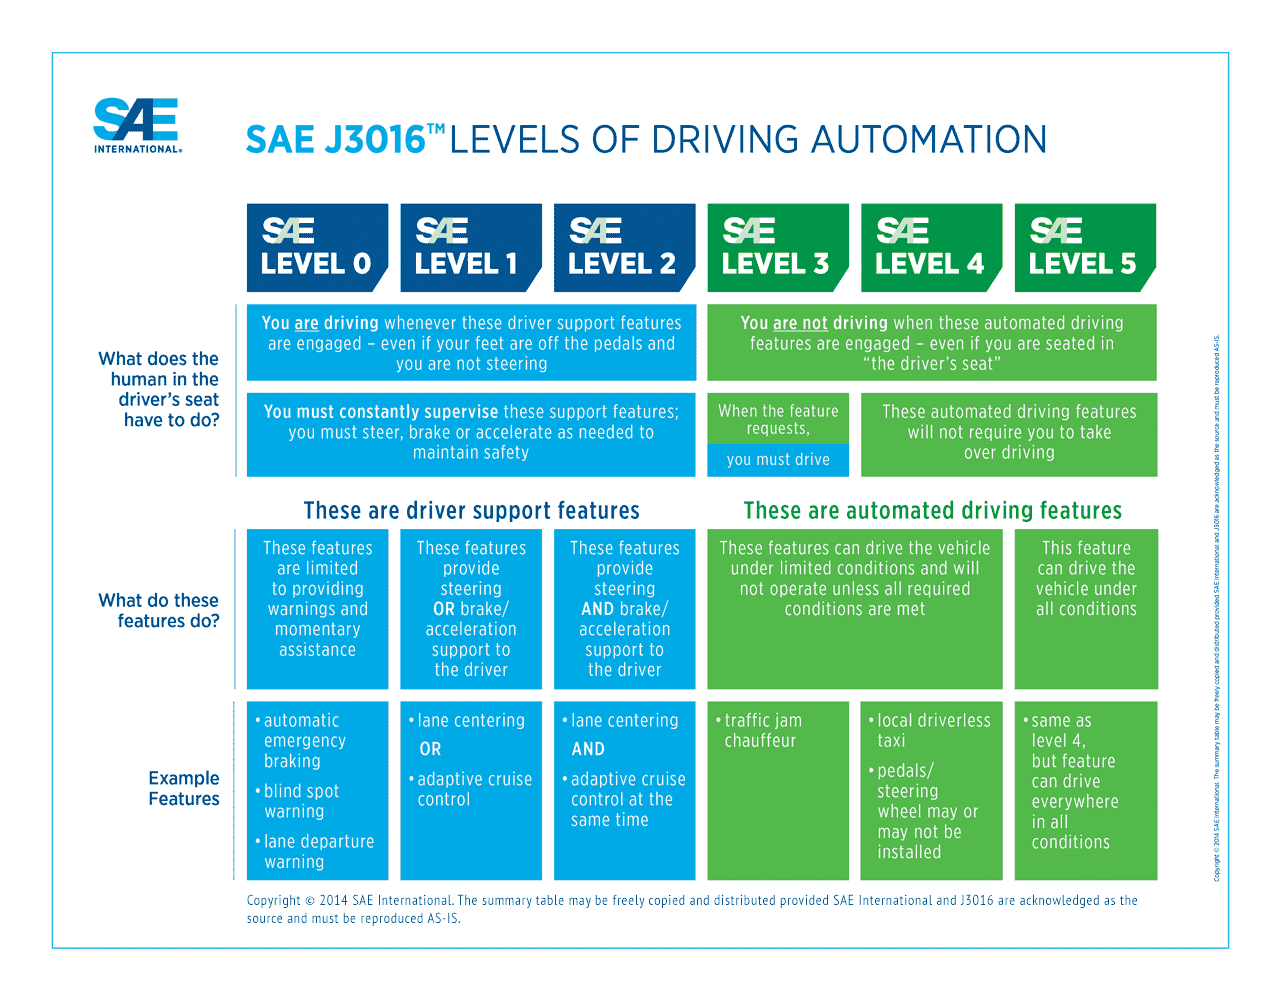
\includegraphics[width=0.9\linewidth]{image/adas_level} \caption{Stufen der Fahrautomatisierung (Shuttleworth, 2019)}\label{fig:unnamed-chunk-37}
\end{figure}

\hypertarget{wichtige-interessensgruppen-34}{%
\subsection*{Wichtige Interessensgruppen}\label{wichtige-interessensgruppen-34}}
\addcontentsline{toc}{subsection}{Wichtige Interessensgruppen}

\begin{itemize}
\tightlist
\item
  \textbf{Betroffene}: Autofahrer:innen, Verkehrsteilnehmer:innen, Versicherungen
\item
  \textbf{Verantwortliche}: Autohersteller
\end{itemize}

\hypertarget{aktueller-stand-der-wissenschaft-und-forschung-34}{%
\subsection*{Aktueller Stand der Wissenschaft und Forschung}\label{aktueller-stand-der-wissenschaft-und-forschung-34}}
\addcontentsline{toc}{subsection}{Aktueller Stand der Wissenschaft und Forschung}

Wichtige Forschungsbereiche im Zusammenhang mit ADAS umfassen \emph{(1)} die technische Verbesserung der Effizienz, Zuverlässigkeit und Funktionalität des Systems (z. B. Storsæter et al., 2021; Capodieci et al., 2021; Tsai et al., 2021; Tian e al., 2021) und \emph{(2)} der menschliche Aspekt der Systemnutzung, bei dem es darum geht, \emph{(a)} wie Informationen über die Fähigkeiten und Grenzen von ADAS vermittelt werden können, damit die Vorteile, die sich aus dem Einsatz in Fahrzeugen ergeben, nicht zunichte gemacht werden, und \emph{(b)} wie die Leistung des Systems in einem bestimmten Kontext die Wahrnehmung des Systems durch Fahrer:innen beeinflusst.

Diese auf den Menschen ausgerichtete Forschung konzentriert sich hauptsächlich auf die Erforschung des Bewusstseins von Fahrer:innen und Fahrzeugkäufer:innen, um die sichere Nutzung von ADAS zu fördern. Dies ist von entscheidender Bedeutung, da eine Studie von Harms et al.~(2020) zeigte, dass viele Geschäftsfahrer:innen nicht wussten, mit welchen ADAS ihr Fahrzeug ausgestattet war, und dass der angegebene Besitz von ADAS (gemessen in einem Fragebogen mit Selbstauskunft) nicht mit dem tatsächlichen Besitz von ADAS übereinstimmte, was den Mangel an Wissen unter den Fahrer:innen belegt. Dies wiederum kann zu einer geringen sozialen Akzeptanz und Nutzbarkeit dieser Sicherheitssysteme in der Praxis führen. Außerdem zeigte eine niederländische Studie, dass Verkäufer:innen und Verbraucher:innen keine zentrale Datenbank für ADAS-Funktionen haben. Infolgedessen erhalten viele Verbraucher:innen keine Informationen über ADAS und/oder können sie am Verkaufsort nicht ausprobieren. Es wurde auch gezeigt, dass unabhängige Autohändler Schwierigkeiten haben, Informationen über ADAS zu erhalten (Boelhouwer et al., 2020).

Im Hinblick auf die Auswirkungen des Kontexts auf die Wahrnehmung von ADAS durch Fahrer:innen zeigte die Studie von Orlovska (2020), dass der Fahrkontext die Nutzung von ADAS aufgrund seiner Leistung stark beeinflusst, was sich folglich auf das Vertrauen der Fahrer:innen und die Bereitschaft, das System langfristig zu nutzen, auswirken kann. Darüber hinaus wurde gezeigt, dass die Entscheidungen der Fahrer:innen über den Einsatz von ADAS während der Fahrt von den aktuellen Fahrbedingungen zum Zeitpunkt der Entscheidungsfindung beeinflusst werden. Diese Ergebnisse zeigen eine Verbindung zwischen dem Kontext, den Fahrer:innen und der Nutzung des ADAS-Systems. Darüber hinaus sind die Hauptergebnisse der Literatur zur Ablenkung der Fahrer:innen und zur Verhaltensanpassung im Zusammenhang mit ADAS, dass \emph{(1)} Fahrer:innen ihr Engagement bei sekundären Aufgaben (sowie ihre Leistung bei diesen Aufgaben) erhöhen, wenn sie mit ADAS fahren, \emph{(2)} das Situationsbewusstsein der Fahrer:innen bei der Nutzung von ADAS geringer ist, \emph{(3)} die Nutzung von ADAS zu längeren Reaktionszeiten, einer größeren Variabilität beim Einhalten der Fahrspur und einer geringeren mentalen Arbeitsbelastung führt. Darüber hinaus wird behauptet, dass Fahrer:innen, die mit Automatisierungssystemen konfrontiert sind, die ihre Erwartungen übertreffen, dazu neigen, den Systemen zu vertrauen und sich ihrer Grenzen nicht bewusst zu sein. Das übermäßige Vertrauen in ADAS erhöht wiederum das Risiko von Kollisionen (Hungund et al., 2021).

Darüber hinaus konzentriert sich ein besonderer Fall von ADAS-Forschung auf ältere Fahrer:innen (Chalkiadakis et al., 2020) und untersucht das Potenzial von ADAS bei der Linderung typischer Beeinträchtigungen wie vermindertes peripheres Sehen, nächtliche Sehprobleme, längere Reaktionszeiten, Fehleinschätzungen von Entfernung und Geschwindigkeit und selektive Aufmerksamkeit. Infolgedessen sind die folgenden Funktionalitäten relevant:

\begin{itemize}
\tightlist
\item
  Erkennung des toten Winkels
\item
  Hinderniserkennungssystem
\item
  Kollisionswarnsystem
\item
  Navigation/Routenführung
\item
  Spurhaltesystem
\item
  Nachtsichtsystem
\item
  Fahrzeuginternes Beschilderungssystem
\item
  System zur Überwachung des Fahrzustandes
\item
  Stau- und Wetterwarnungen
\end{itemize}

Darüber hinaus zeigte die Studie von Zahabi et al.~(2021), dass ein auf Demonstrationen basierendes Training für ADAS für ältere Männer effektiver ist, während ein videobasiertes Training für ältere Frauen effektiver ist.

\hypertarget{aktueller-stand-der-praktischen-umsetzung-34}{%
\subsection*{Aktueller Stand der praktischen Umsetzung}\label{aktueller-stand-der-praktischen-umsetzung-34}}
\addcontentsline{toc}{subsection}{Aktueller Stand der praktischen Umsetzung}

Es wird allgemein behauptet, dass wir in der Praxis derzeit die Automatisierungsstufe 2 (nach SAE-Klassifizierung, siehe Tabelle oben) erreicht haben, bei der das Fahrzeug zwar lenken und beschleunigen kann, aber immer noch nicht selbst fährt und Fahrer:innen die volle Verantwortung für das Fahrzeug tragen. Eine kürzlich von \href{https://www.rolandberger.com/en/Insights/Publications/Advanced-Driver-Assistance-Systems-A-ubiquitous-technology-for-the-future-of.html}{Roland Berger} durchgeführte Umfrage unter 80 globalen Herstellern, Automobilexperten, Zulieferern und 3.000 Fahrer:innen zeigt, dass 85 \% der im Jahr 2025 weltweit produzierten Fahrzeuge mit mindestens Stufe 1 der Fahrautomatisierung ausgestattet sein werden. Gleichzeitig wird nicht damit gerechnet, dass bis dahin mehr als 1 \% der Fahrzeuge mit der Automatisierungsstufe 4 oder 5 ausgestattet sein werden (Shirokinskiy et al., 2021).

Darüber hinaus hat sich gezeigt, dass die derzeitige Pandemie die Gesamtentwicklung bei ADAS-Systemen verlangsamt und in einigen Fällen -17 \% erreicht (Shirokinskiy et al., 2021). Eine weitere Herausforderung für die Industrie ist das Fehlen einer standardisierten Nomenklatur für ADAS-Funktionen, was einerseits die Verfolgung dieser Funktionen erschwert und andererseits das Verständnis der Fahrer:innen für die Funktionen erschwert. So ist beispielsweise die adaptive Geschwindigkeitsregelung (ACC) in Fahrzeugen von Fiat, Ford, Volkswagen und Peugeot als Adaptive Cruise Control, in Citroen und BMW als Intelligent Cruise Control und in Mercedes als DISTRONIC bekannt (Helman \& Carsten, 2019). Im Mai 2020 gab die SAE eine \href{https://www.repairerdrivennews.com/2020/05/15/sae-international-endorses-generic-adas-terminology-recommendations/}{allgemeine ADAS-Terminologieempfehlung} heraus, um Standardisierungsprobleme zu lösen (Huetter, 2020).

\hypertarget{relevante-initiativen-in-uxf6sterreich-34}{%
\subsection*{Relevante Initiativen in Österreich}\label{relevante-initiativen-in-uxf6sterreich-34}}
\addcontentsline{toc}{subsection}{Relevante Initiativen in Österreich}

\begin{itemize}
\tightlist
\item
  \href{https://www.alp-lab.at/}{Alp-lab}
\item
  \href{https://www.smartmicro.com/press-media/detail/smartmicro-sensors-deployed-in-austria}{Smartmicro.com}
\end{itemize}

\hypertarget{auswirkungen-in-bezug-auf-die-ziele-fuxfcr-nachhaltige-entwicklung-sdgs-34}{%
\subsection*{Auswirkungen in Bezug auf die Ziele für nachhaltige Entwicklung (SDGs)}\label{auswirkungen-in-bezug-auf-die-ziele-fuxfcr-nachhaltige-entwicklung-sdgs-34}}
\addcontentsline{toc}{subsection}{Auswirkungen in Bezug auf die Ziele für nachhaltige Entwicklung (SDGs)}

\begin{longtable}[]{@{}ccccc@{}}
\toprule
\begin{minipage}[b]{0.17\columnwidth}\centering
Ebene der Auswirkungen\strut
\end{minipage} & \begin{minipage}[b]{0.16\columnwidth}\centering
Indikator\strut
\end{minipage} & \begin{minipage}[b]{0.17\columnwidth}\centering
Richtung der Auswirkungen\strut
\end{minipage} & \begin{minipage}[b]{0.17\columnwidth}\centering
Beschreibung des Ziels \& SDG\strut
\end{minipage} & \begin{minipage}[b]{0.17\columnwidth}\centering
Quelle\strut
\end{minipage}\tabularnewline
\midrule
\endhead
\begin{minipage}[t]{0.17\columnwidth}\centering
Individuell\strut
\end{minipage} & \begin{minipage}[t]{0.16\columnwidth}\centering
ADAS mildert die Auswirkungen altersbedingter Beeintraechtigungen\strut
\end{minipage} & \begin{minipage}[t]{0.17\columnwidth}\centering
\textbf{+}\strut
\end{minipage} & \begin{minipage}[t]{0.17\columnwidth}\centering
Gesundheit und Wohlbefinden (\emph{3})\strut
\end{minipage} & \begin{minipage}[t]{0.17\columnwidth}\centering
Chalkiadakis et al., 2020\strut
\end{minipage}\tabularnewline
\begin{minipage}[t]{0.17\columnwidth}\centering
Individuell\strut
\end{minipage} & \begin{minipage}[t]{0.16\columnwidth}\centering
Erleichtert die Mobilitaet fuer aeltere Fahrer:innen\strut
\end{minipage} & \begin{minipage}[t]{0.17\columnwidth}\centering
\textbf{+}\strut
\end{minipage} & \begin{minipage}[t]{0.17\columnwidth}\centering
Gleichheit (\emph{5,10})\strut
\end{minipage} & \begin{minipage}[t]{0.17\columnwidth}\centering
Chalkiadakis et al., 2020\strut
\end{minipage}\tabularnewline
\begin{minipage}[t]{0.17\columnwidth}\centering
Systemisch\strut
\end{minipage} & \begin{minipage}[t]{0.16\columnwidth}\centering
Erhoeht den Fahrkomfort, aber es gibt kaum eindeutige Beweise fuer die Auswirkungen auf die Sicherheit\strut
\end{minipage} & \begin{minipage}[t]{0.17\columnwidth}\centering
\textbf{\textasciitilde{}}\strut
\end{minipage} & \begin{minipage}[t]{0.17\columnwidth}\centering
Gesundheit und Wohlbefinden (\emph{3})\strut
\end{minipage} & \begin{minipage}[t]{0.17\columnwidth}\centering
Sullivan et al., 2016\strut
\end{minipage}\tabularnewline
\begin{minipage}[t]{0.17\columnwidth}\centering
Systemisch\strut
\end{minipage} & \begin{minipage}[t]{0.16\columnwidth}\centering
Globale Trends in der ADAS-F\&E\strut
\end{minipage} & \begin{minipage}[t]{0.17\columnwidth}\centering
\textbf{+}\strut
\end{minipage} & \begin{minipage}[t]{0.17\columnwidth}\centering
Innovation und Infrastruktur (\emph{9})\strut
\end{minipage} & \begin{minipage}[t]{0.17\columnwidth}\centering
Yochman, 2020\strut
\end{minipage}\tabularnewline
\bottomrule
\end{longtable}

\hypertarget{technologie--und-gesellschaftlicher-bereitschaftsgrad-30}{%
\subsection*{Technologie- und gesellschaftlicher Bereitschaftsgrad}\label{technologie--und-gesellschaftlicher-bereitschaftsgrad-30}}
\addcontentsline{toc}{subsection}{Technologie- und gesellschaftlicher Bereitschaftsgrad}

\begin{longtable}[]{@{}cc@{}}
\toprule
Stand der Technologiebereitschaft & Gesellschaftlicher Bereitschaftsgrad\tabularnewline
\midrule
\endhead
7-9 & 6-8\tabularnewline
\bottomrule
\end{longtable}

\hypertarget{offene-fragen-32}{%
\subsection*{Offene Fragen}\label{offene-fragen-32}}
\addcontentsline{toc}{subsection}{Offene Fragen}

\begin{enumerate}
\def\labelenumi{\arabic{enumi}.}
\tightlist
\item
  Wie kann eine Standardisierung der ADAS-Nomenklatur gefördert und erreicht werden?
\item
  Wie können die Auswirkungen der Verhaltensanpassung in größerem Umfang in die Gestaltung von ADAS einbezogen werden?
\end{enumerate}

\hypertarget{weitere-links-28}{%
\subsection{Weitere links}\label{weitere-links-28}}

\begin{itemize}
\tightlist
\item
  \href{https://ec.europa.eu/transport/road_safety/sites/default/files/pdf/ersosynthesis2018-adas.pdf}{ec.europa.eu}
\item
  \href{https://aaafoundation.org/wp-content/uploads/2017/12/BehavioralAdaptationADAS.pdf}{aaafoundation.org}
\end{itemize}

\hypertarget{referenzen-34}{%
\subsection*{Referenzen}\label{referenzen-34}}
\addcontentsline{toc}{subsection}{Referenzen}

\begin{itemize}
\tightlist
\item
  Boelhouwer, A., Van den Beukel, A. P., Van der Voort, M. C., Hottentot, C., De Wit, R. Q., \& Martens, M. H. (2020). How are car buyers and car sellers currently informed about ADAS? An investigation among drivers and car sellers in the Netherlands. Transportation Research Interdisciplinary Perspectives, 4, 100103.
\item
  Capodieci, N., Cavicchioli, R., Muzzini, F., \& Montagna, L. (2021). Improving emergency response in the era of ADAS vehicles in the Smart City. ICT Express.
\item
  Chalkiadakis, C., Mitsakis, E., \& Tzanis, D. (2020, September). Requirements for the development and implementation of ADAS and C-ITS services for older drivers. In 2020 IEEE 23rd International Conference on Intelligent Transportation Systems (ITSC) (pp.~1-6). IEEE.
\item
  Harms, I. M., Bingen, L., \& Steffens, J. (2020). Addressing the awareness gap: A combined survey and vehicle registration analysis to assess car owners' usage of ADAS in fleets. Transportation Research Part A: Policy and Practice, 134, 65-77.
\item
  Helman, S. \& Carsten, O. (2019) What does my car do? Available at: \url{https://www.pacts.org.uk/wp-content/uploads/What-does-my-car-do-2.1_.pdf} {[}Accessed: 31 May 2021{]}.
\item
  Huetter, J. (2020) SAE International endorses generic ADAS terminology recommendations. Available at \textless{} \url{https://www.repairerdrivennews.com/2020/05/15/sae-international-endorses-generic-adas-terminology-recommendations/}\textgreater{} Accessed: 31/05/2021
\item
  Hungund, A. P., Pai, G., \& Pradhan, A. K. (2021). Systematic Review of Research on Driver Distraction in the Context of Advanced Driver Assistance Systems. Transportation Research Record, 03611981211004129.
\item
  Orlovska, J., Novakazi, F., Lars-Ola, B., Karlsson, M., Wickman, C., \& Söderberg, R. (2020). Effects of the driving context on the usage of Automated Driver Assistance Systems (ADAS)-Naturalistic Driving Study for ADAS evaluation. Transportation research interdisciplinary perspectives, 4, 100093.
\item
  Samsara.com (2020). Advanced Driver Assistance Systems (ADAS) for Commercial Fleets. Available at:\textless{} \url{https://www.samsara.com/guides/adas}\textgreater{} {[}Accessed: 28 April 2021{]}.
\item
  Shirokinskiy, K., Bernhart, W. and Keese, S., 2021. Advanced Driver-Assistance Systems: A ubiquitous technology for the future of vehicles. Roland Berger. Available at: \url{https://www.rolandberger.com/en/Insights/Publications/Advanced-Driver-Assistance-Systems-A-ubiquitous-technology-for-the-future-of.html} {[}Accessed: 31 May 2021{]}.
\item
  Shuttleworth, J. (2019). SAE Standards News: J3016 automated-driving graphic update. Available at: \url{https://www.sae.org/news/2019/01/sae-updates-j3016-automated-driving-graphic} {[}Accessed: 28 April 2021{]}.
\item
  Storsæter, A. D., Pitera, K., \& McCormack, E. (2021). Using ADAS to Future-Proof Roads---Comparison of Fog Line Detection from an In-Vehicle Camera and Mobile Retroreflectometer. Sensors, 21(5), 1737.
\item
  Sullivan, J. M., Flannagan, M. J., Pradhan, A. K., \& Bao, S. (2016). Literature review of behavioral adaptations to advanced driver assistance systems.
\item
  Tian, J., Liu, S., Zhong, X., \& Zeng, J. (2021). LSD-based adaptive lane detection and tracking for ADAS in structured road environment. Soft Computing, 25(7), 5709-5722.
\item
  Tsai, W. C., Lai, J. S., Chen, K. C., M Shivanna, V., \& Guo, J. I. (2021). A lightweight motional object behavior prediction system harnessing deep learning technology for embedded adas applications. Electronics, 10(6), 692.
\item
  Yochman, F. (2020) Top automakers with highest ADAS and autonomous vehicles R\&D spending. Available at: \textless{} \url{https://m14intelligence.com/public/index.php/blog/34}\textgreater{} {[}Accessed: 31 April 2021{]}.
\item
  Zahabi, M., Razak, A. M. A., Mehta, R. K., \& Manser, M. (2021). Effect of advanced driver-assistance system trainings on driver workload, knowledge, and trust. Transportation research part F: traffic psychology and behaviour, 76, 309-320.
\end{itemize}

\hypertarget{parking_assistance}{%
\section{Einparkhilfe-System}\label{parking_assistance}}

\hypertarget{definition-35}{%
\subsection*{Definition}\label{definition-35}}
\addcontentsline{toc}{subsection}{Definition}

Heutzutage wird das Einparken von Autos zu einer immer schwierigeren Aufgabe, da die Fahrzeuge immer größer werden und die Sicht nach hinten und vorne immer schlechter wird. Außerdem nimmt die Zahl der Fahrzeuge auf der Straße weiter zu, was die Suche nach Parkplätzen erschwert. Um diese Herausforderung zu bewältigen, sind effiziente und fortschrittliche Einparktechniken erforderlich, die z. B. den richtigen Parkplatz finden und Autos effizient einparken (Khalid et al., 2021).
Während in den 1990er Jahren Einparkhilfesysteme nicht als notwendig erachtet wurden, sind Systeme, die den Einparkvorgang unterstützen, heute Standard in neuen Fahrzeugen und haben eine hohe Akzeptanzrate. Während Parkassistenzsysteme der ersten Generationen vor allem informativ waren, helfen diese Systeme heute bei der Suche nach einer geeigneten Parklücke und unterstützen die Lenkung während des Einparkmanövers. Zukünftige Systeme werden noch automatisierter werden, bis hin zu dem Punkt, dass sie ihren Parkplatz ohne menschliches Zutun finden (Automated Valet Parking) (Gotzig, 2016).

Im Hinblick auf die Sicherheit können Parkassistenzsysteme Versicherungsschäden, die bei Einparkmanövern auftreten, um 30 \% reduzieren (ADAC, 2020). Außerdem bieten sie mit dem Notbremsassistenten eine nützliche Anwendung, die Unfälle mit anderen Verkehrsteilnehmer:innen beim Rückwärtsfahren verhindert (ADAC, 2019).

Moderne Einparkassistenten arbeiten mit zwei Sensorkonzepten: Ultraschallsensoren für den Nahbereich am Heck (oft schon als ``Parkpiepser'' eingebaut) und Radarsensoren mit größerer Reichweite seitlich im Stoßfänger (ADAC, 2019). Zusätzlich gibt es auch Neuerscheinungen mit 360°-Sicht um das Auto herum (Land Rover, ohne Datum; Mercedes-Benz, ohne Datum). Allerdings gibt es dazu derzeit noch keine Tests.

\hypertarget{wichtige-interessensgruppen-35}{%
\subsection*{Wichtige Interessensgruppen}\label{wichtige-interessensgruppen-35}}
\addcontentsline{toc}{subsection}{Wichtige Interessensgruppen}

\begin{itemize}
\tightlist
\item
  \textbf{Betroffene}: Autofahrer:innen, Verkehrsteilnehmer:innen, Versicherungen
\item
  \textbf{Verantwortliche}: Autohersteller
\end{itemize}

\hypertarget{aktueller-stand-der-wissenschaft-und-forschung-35}{%
\subsection*{Aktueller Stand der Wissenschaft und Forschung}\label{aktueller-stand-der-wissenschaft-und-forschung-35}}
\addcontentsline{toc}{subsection}{Aktueller Stand der Wissenschaft und Forschung}

Die Forschung im Bereich der bordeigenen Parksysteme wird fast ausschließlich von den Automobilherstellern betrieben. Die Forschung konzentriert sich eher auf größere Themen wie die Verfolgung des Standorts des Fahrzeugs, Platzbuchungssysteme mit Hilfe des Internet der Dinge und Staus, die durch \emph{Parkkreuzungen} verursacht werden.
Darüber hinaus werden Tests zur Verschmelzung von Notbremsassistent und Einparkassistent durchgeführt, um die Schwierigkeiten bei der Hinderniserkennung zu überwinden und die Kollisionsrate in dieser speziellen Situation zu verringern. Der ADAC hat die AEB-Systeme (Autonomated Emergency Braking) von Mercedes, Volvo, BMW, Seat und Skoda in drei Testszenarien getestet: \emph{(1)} ein Fußgänger -Dummy steht hinter einem Auto oder geht vorbei, \emph{(2)} ein Auto parkt in Fahrtrichtung und \emph{(3)} Radfahrer sowie Autos fahren quer vorbei.
BMW reagierte in allen Situationen am besten mit Radar und Ultraschall - mit einigen Aussetzern, vor allem bei sich bewegenden Fußgänger:innen oder Querverkehr. Der Mercedes hingegen nutzte seine seitlichen Radarsensoren nur zum Rückwärtsbremsen und erkannte daher stehende Fahrzeuge gar nicht. Das VW-System von Skoda und Seat verfügte zwar über Radar und Ultraschall, aber bewegte Fußgänger:innen wurden nur zufällig oder gar nicht erkannt.
Insgesamt zeigten diese Tests, dass die automatisch bremsenden Einparkassistenten zwar viel Potenzial haben, aber noch lange nicht optimal sind. Selbst die Systeme der Spitzenreiter arbeiten noch nicht 100\%ig zuverlässig. Aber auch die preiswerten Ultraschallsensoren können sehr effektiv sein und sogar Fußgängerkollisionen verhindern, wie der BMW im Test zeigte. Deshalb ist es wichtig, dass die Hersteller ihre Fahrzeuge serienmäßig mit einem wirksamen AEB-System ausstatten. Die notwendige Technik ist in den meisten Pkw bereits vorhanden, wobei die hinteren Ultraschallsensoren mit der Bremsfunktion verknüpft werden müssten (ADAC, 2019).
Die größten Schwierigkeiten treten bei der Fußgängererkennung auf, also in den Szenarien, in denen das Risiko von Personenschäden potenziell am höchsten ist. Einige der getesteten Fahrzeuge erkannten die Gefahrensituation zu spät oder gar nicht.

\hypertarget{aktueller-stand-der-praktischen-umsetzung-35}{%
\subsection*{Aktueller Stand der praktischen Umsetzung}\label{aktueller-stand-der-praktischen-umsetzung-35}}
\addcontentsline{toc}{subsection}{Aktueller Stand der praktischen Umsetzung}

Fast 50 Prozent der Autos in Deutschland sind inzwischen mit Einparkhilfen ausgestattet. Dennoch zeigen die Ergebnisse einer Studie der HUK-Coburg, Deutschlands größter Kfz-Versicherung mit elf Millionen versicherten Autos, dass die Zahl der Blechschäden nicht zurückgegangen ist und die Schadenskosten sogar leicht gestiegen sind. Grund dafür ist die Beschädigung des teuren, im Stoßfänger integrierten Sensors der Park Distance Control (PDC), wenn das Fahrzeug beim Einparken auf ein Hindernis prallt (Focus Online, 2017).
Im Jahr 2017 ereigneten sich in Österreich 570 Unfälle mit Personenschaden beim Rückwärtsfahren mit Pkw. Dabei gab es keine Todesopfer, aber rund 290 Personen wurden verletzt, 60 davon schwer. Hinzu kommt ein hoher Anteil an Sachschäden durch das Übersehen von Hindernissen (ÖAMTC, 2019).
Unterschiedlichen Quellen zufolge sind zwischen 23\% und 46\% der Autos in Deutschland mit einem On-Board-Parkassistenten ausgestattet (Focus Online, 2017). Dagegen sind nur 13 \% der Fahrzeuge mit einem Notbremsassistenten ausgestattet, der bei einer drohenden Kollision mit dem vorausfahrenden Fahrzeug automatisch bremst oder sogar Fußgänger:innen und Radfahrer:innen erkennt. Eine vom Deutschen Verkehrssicherheitsrat durchgeführte Umfrage unter 1.000 Befragten ergab, dass 85 \% der Befragten den Notbremsassistenten als sehr nützlich und 65 \% den Parkassistenten als sehr nützlich einstufen (Handelsblatt, 2016).
Die derzeit fortschrittlichste Technologie in Bezug auf die Einparkhilfe bietet der Tesla S. Das System ist völlig automatisiert und ermöglicht es dem Auto, sich selbst aus einer engen Lücke herauszufahren, ohne dass Fahrer:innen eingreifen müssen. Es ist jedoch davon auszugehen, dass die Technologie auch von anderen Herstellern angeboten wird und sich in den kommenden Jahren rasch verbessern wird. Ein Grund dafür ist, dass Einparkassistenten mit Bremseingriff ab 2020 Teil des europäischen Fahrzeugtestprogramms Euro NCAP sein werden. In der Vergangenheit hat sich gezeigt, dass die Aufnahme von aktiven und passiven Pkw-Sicherheitssystemen in dieses Programm die Ausstattungsrate der Fahrzeuge rasch erhöht (ÖAMTC, 2019).

\hypertarget{relevante-initiativen-in-uxf6sterreich-35}{%
\subsection*{Relevante Initiativen in Österreich}\label{relevante-initiativen-in-uxf6sterreich-35}}
\addcontentsline{toc}{subsection}{Relevante Initiativen in Österreich}

\begin{itemize}
\tightlist
\item
  \href{https://www.oeamtc.at/tests/assistenzsystemtest/fuenf-parkassistenten-mit-notbremssystem-im-test-31717317}{oeamtc.at}
\end{itemize}

\hypertarget{auswirkungen-in-bezug-auf-die-ziele-fuxfcr-nachhaltige-entwicklung-sdgs-35}{%
\subsection*{Auswirkungen in Bezug auf die Ziele für nachhaltige Entwicklung (SDGs)}\label{auswirkungen-in-bezug-auf-die-ziele-fuxfcr-nachhaltige-entwicklung-sdgs-35}}
\addcontentsline{toc}{subsection}{Auswirkungen in Bezug auf die Ziele für nachhaltige Entwicklung (SDGs)}

\begin{longtable}[]{@{}ccccc@{}}
\toprule
\begin{minipage}[b]{0.17\columnwidth}\centering
Ebene der Auswirkungen\strut
\end{minipage} & \begin{minipage}[b]{0.16\columnwidth}\centering
Indikator\strut
\end{minipage} & \begin{minipage}[b]{0.17\columnwidth}\centering
Richtung der Auswirkungen\strut
\end{minipage} & \begin{minipage}[b]{0.17\columnwidth}\centering
Beschreibung des Ziels \& SDG\strut
\end{minipage} & \begin{minipage}[b]{0.17\columnwidth}\centering
Quelle\strut
\end{minipage}\tabularnewline
\midrule
\endhead
\begin{minipage}[t]{0.17\columnwidth}\centering
Individuell\strut
\end{minipage} & \begin{minipage}[t]{0.16\columnwidth}\centering
Weniger Verkehrsunfaelle beim Parken\strut
\end{minipage} & \begin{minipage}[t]{0.17\columnwidth}\centering
\textbf{+}\strut
\end{minipage} & \begin{minipage}[t]{0.17\columnwidth}\centering
Gesundheit und Wohlbefinden (\emph{3})\strut
\end{minipage} & \begin{minipage}[t]{0.17\columnwidth}\centering
ADAC, 2019\strut
\end{minipage}\tabularnewline
\begin{minipage}[t]{0.17\columnwidth}\centering
Individuell\strut
\end{minipage} & \begin{minipage}[t]{0.16\columnwidth}\centering
Hoehere Kosten im Falle einer Kollision\strut
\end{minipage} & \begin{minipage}[t]{0.17\columnwidth}\centering
\textbf{-}\strut
\end{minipage} & \begin{minipage}[t]{0.17\columnwidth}\centering
Nachhaltige wirtschaftliche Entwicklung (\emph{8,11})\strut
\end{minipage} & \begin{minipage}[t]{0.17\columnwidth}\centering
Focus Online, 2017\strut
\end{minipage}\tabularnewline
\begin{minipage}[t]{0.17\columnwidth}\centering
Systemisch\strut
\end{minipage} & \begin{minipage}[t]{0.16\columnwidth}\centering
Neue Konzepte getestet\strut
\end{minipage} & \begin{minipage}[t]{0.17\columnwidth}\centering
\textbf{+}\strut
\end{minipage} & \begin{minipage}[t]{0.17\columnwidth}\centering
Innovation und Infrastruktur (\emph{9})\strut
\end{minipage} & \begin{minipage}[t]{0.17\columnwidth}\centering
Euro NCAP, 2021\strut
\end{minipage}\tabularnewline
\bottomrule
\end{longtable}

\hypertarget{technologie--und-gesellschaftlicher-bereitschaftsgrad-31}{%
\subsection*{Technologie- und gesellschaftlicher Bereitschaftsgrad}\label{technologie--und-gesellschaftlicher-bereitschaftsgrad-31}}
\addcontentsline{toc}{subsection}{Technologie- und gesellschaftlicher Bereitschaftsgrad}

\begin{longtable}[]{@{}cc@{}}
\toprule
Stand der Technologiebereitschaft & Gesellschaftlicher Bereitschaftsgrad\tabularnewline
\midrule
\endhead
8-9 & 8-9\tabularnewline
\bottomrule
\end{longtable}

\hypertarget{offene-fragen-33}{%
\subsection*{Offene Fragen}\label{offene-fragen-33}}
\addcontentsline{toc}{subsection}{Offene Fragen}

\begin{enumerate}
\def\labelenumi{\arabic{enumi}.}
\tightlist
\item
  Wie können die Akzeptanz und die Benutzerfreundlichkeit bei Fahrer:innen, insbesondere bei älteren Menschen, erhöht werden?
\item
  Welche rechtlichen Auswirkungen hat die Nutzung des assistierten Parkens sowohl für die Fahrer:innen als auch für die Automobilhersteller?
\end{enumerate}

\hypertarget{referenzen-35}{%
\subsection*{Referenzen}\label{referenzen-35}}
\addcontentsline{toc}{subsection}{Referenzen}

\begin{itemize}
\tightlist
\item
  ADAC. (2019, May 14). Parkassistenten im Test: Noch nicht gut genug. \url{https://presse.adac.de/meldungen/adac-ev/tests/parkassistent.html}
\item
  ADAC. (2020, January 9). Fahrerassistenzsysteme im Überblick \textbar{} ADAC. \url{https://www.adac.de/rund-ums-fahrzeug/ausstattung-technik-zubehoer/assistenzsysteme/fahrerassistenzsysteme/}
\item
  Euro NCAP. (2021). \url{http://www.euroncap.com} (Accessed: 26 February 2021)
\item
  Focus Online. (2017, April 27). Einparkhilfen bringen nichts - sondern verursachen mehr Schaden - FOCUS Online. \url{https://www.focus.de/auto/news/untersuchung-der-huk-coburg-studie-einparkhilfe-hilft-nicht-sie-versucht-eher-mehr-schaden_id_7035248.html}
\item
  Gotzig, H. (2016). Parking Assistance. In H. Winner, S. Hakuli, F. Lotz, \& C. Singer (Eds.), Handbook of Driver Assistance Systems: Basic Information, Components and Systems for Active Safety and Comfort (pp.~1077--1092). Springer International Publishing. \url{https://doi.org/10.1007/978-3-319-12352-3_45}
\item
  Handelsblatt. (2016, April 8). Umfrage zu Assistenzsystemen\,: Einparkassistent nützlich, Notbremsassistent nützlicher. \url{https://www.handelsblatt.com/auto/nachrichten/umfrage-zu-assistenzsystemen-einparkassistent-nuetzlich-notbremsassistent-nuetzlicher/13404708.html?ticket=ST-4955434-naHBLAxI66h66nbvrBXF-ap1}
\item
  Khalid, M., Wang, K., Aslam, N., Cao, Y., Ahmad, N., \& Khan, M. K. (2021). From smart parking towards autonomous valet parking: A survey, challenges and future Works. Journal of Network and Computer Applications, 175, 102935. \url{https://doi.org/https://doi.org/10.1016/j.jnca.2020.102935}
\item
  Land Rover. (n.d.). Parking Assistance \textbar{} InControl \textbar{} Land Rover UK. Available at: \url{https://www.landrover.co.uk/incontrol/driver-safety-and-assistance/parking-assistance.html} {[}Accessed: 25 February 2021{]}
\item
  Margreiter, M., Mayer, P., Alpas, M., \& Vlahogianni, E. (2017). Driver's Willingness to Use Parking Assistance Tools and their Expectations: A Case Study for the Cities of Munich and Athens. In 8th International Congress on Transportation Research.
\item
  Mercedes-Benz. (n.d.). Mercedes-Benz X-Klasse: Park-Paket mit 360°-Kamera. Available at: \url{https://www.mercedes-benz.at/passengercars/mercedes-benz-cars/models/x-class/x-class-pickup/facts-and-lines/equipment-packages/360-camera.html} {[}Accessed: 25 February 2021{]}
\item
  Tsugawa, S. (2006). Trends and issues in safe driver assistance systems: Driver acceptance and assistance for elderly drivers. IATSS research, 30(2), 6-18.
\item
  ÖAMTC. (2019, May 14). ÖAMTC: Fünf Parkassistenten mit Notbremssystem im Test (+ Fotos, + Grafik) \textbar{} ÖAMTC, 14.05.2019. \url{https://www.ots.at/presseaussendung/OTS_20190514_OTS0021/oeamtc-fuenf-parkassistenten-mit-notbremssystem-im-test-fotos-grafik}
\end{itemize}

\hypertarget{lane_keeping}{%
\section{Spurhalte-Assistent}\label{lane_keeping}}

\hypertarget{synonyme-30}{%
\subsection*{Synonyme}\label{synonyme-30}}
\addcontentsline{toc}{subsection}{Synonyme}

\emph{Spurhalte-Assistent (LKAS - Lane Keeping Assist System), Spurhalte-Assistent (LKA)}

\hypertarget{definition-36}{%
\subsection*{Definition}\label{definition-36}}
\addcontentsline{toc}{subsection}{Definition}

Der Spurhalteassistent überwacht die Fahrbahnmarkierungen und verwendet in der Regel eine Kamera hinter der Windschutzscheibe, um das Fahrzeug in der Fahrspur zu halten und so die Fahrer:innen zu entlasten. Derzeit gibt es verschiedene Systeme, die nicht alle gleich sind (Autonationdrive, 2019):

\begin{itemize}
\tightlist
\item
  \textbf{Spurhalteassistent (Lane Departure Warning, LDW)}: Akustische oder visuelle Warnungen signalisieren den Fahrer:innen, dass sich das Fahrzeug den Fahrbahnmarkierungen nähert oder diese überqueren könnte.
\item
  \textbf{Road Departure Assist (RDA)}: Ein automatisches Lenksystem, das auch ein automatisches Bremssystem umfassen kann, hält das Fahrzeug auf der Fahrbahn.
\item
  \textbf{Spurhalte-Assistent (Lane Keeping Assist - LKA)}: Ein automatisches Lenksystem, das auch ein automatisches Bremssystem enthalten kann, hält das Fahrzeug in der Fahrspur.
\item
  \textbf{Spurführungsassistent (Lane Centering Assist - LCA)}: Ein automatisches Lenksystem, das auch ein automatisches Bremssystem umfassen kann, um das Fahrzeug in der Mitte der Fahrspur zu halten.
\end{itemize}

Der Hauptunterschied zwischen diesen beiden Systemen besteht darin, dass der LDW die Fahrer:innen beim Überfahren der Fahrbahnmarkierung durch verschiedene sensorische Hinweise wie taktile, visuelle oder akustische Signale informiert, während der LKAS die Fahrer:innen durch die Anpassung der Lenkradbewegungen in Abhängigkeit vom Abstand zur Fahrbahnmarkierung auf beiden Seiten dabei unterstützt, in der Fahrspur zu bleiben. Die Systeme können reaktiv oder proaktiv arbeiten, d.~h. das Fahrzeug wird reaktiv auf die Spur zurückgeführt, wenn es beginnt, die Fahrspur zu verlassen, bzw. proaktiv in der Mitte der Fahrspur gehalten. Es wird in der Regel von den Fahrer:innen aktiviert und funktioniert bei Geschwindigkeiten zwischen 65 km/h und 180 km/h und einem Radius von 230 m. Daher eignet es sich am besten für Autobahnen und Schnellstraßen, weniger jedoch für Stadt- oder Landstraßen. Auch wenn das LKAS aktiviert ist, bleiben Fahrer:innen für die Kontrolle des Fahrzeugs verantwortlich. Daher prüft LKAS ständig, welche Lenkbewegungen Fahrer:innen ausführen und sie die Hände am Lenkrad hatten. Stellt das System fest, dass Fahrer:innen nicht aktiv lenken, gibt es eine Warnung aus und schaltet sich ab. Auf diese Weise wird sichergestellt, dass Fahrer:innen stets die Kontrolle über das Fahrzeug behalten. Außerdem können Fahrer:innen das LKAS jederzeit außer Kraft setzen. So deaktiviert sich LKAS zum Beispiel automatisch beim Bremsen und beim absichtlichen Aufladen der Fahrspur durch den Einsatz von Blinkern (VDA, 2021).

\hypertarget{wichtige-interessensgruppen-36}{%
\subsection*{Wichtige Interessensgruppen}\label{wichtige-interessensgruppen-36}}
\addcontentsline{toc}{subsection}{Wichtige Interessensgruppen}

\begin{itemize}
\tightlist
\item
  \textbf{Betroffene}: Allgemeinheit, Autofahrer:innen, Straßeninfrastrukturunternehmen, Versicherungen
\item
  \textbf{Verantwortliche}: Automobilhersteller, Verkehrsbehörden, nationale Regierungen und internationale Einrichtungen (z. B. EU oder \href{https://unece.org/fileadmin/DAM/trans/main/wp29/wp29regs/2018/R079r4e.pdf}{UNECE})
\end{itemize}

\hypertarget{aktueller-stand-der-wissenschaft-und-forschung-36}{%
\subsection*{Aktueller Stand der Wissenschaft und Forschung}\label{aktueller-stand-der-wissenschaft-und-forschung-36}}
\addcontentsline{toc}{subsection}{Aktueller Stand der Wissenschaft und Forschung}

In der aktuellen Forschung werden neue Ansätze für die Entwicklung von Spurhalteassistenten erforscht, wie etwa der Einsatz des globalen Satellitennavigationssystems (Tominaga et al., 2020), Deep Learning (Wang et al., 2020) oder neuronale Netztechniken (Yusuf et al., 2020). Darüber hinaus zielt sie auf die Validierung und Verbesserung von LKAS ab, indem sie die Auswirkungen des Systemdesigns (Lee et al., 2018) und unterschiedlicher Straßenbedingungen auf die Gesamtqualität der Spurhalteassistenz untersucht (Romano et al., 2020). Darüber hinaus wurde in einer Reihe von Studien das Potenzial der Einbeziehung von Fahrereigenschaften zur Entwicklung eines personalisierten Spurhalteassistenten untersucht. Eine weitere Studie von Weaver \& Gonzalez (2020) konzentrierte sich auf den Einfluss von LKAS auf das Verhalten der Fahrer:innen und die Akzeptanz der LKAS-Technologie. Sie bestätigte nicht nur bestehende Erkenntnisse, dass mehr Erfahrung und Vertrautheit mit dem System die Akzeptanz und das Vertrauen erhöhen, sondern zeigte auch eine positive Reaktion von Personen, die noch keine Erfahrung mit LKAS hatten.

\hypertarget{aktueller-stand-der-praktischen-umsetzung-36}{%
\subsection*{Aktueller Stand der praktischen Umsetzung}\label{aktueller-stand-der-praktischen-umsetzung-36}}
\addcontentsline{toc}{subsection}{Aktueller Stand der praktischen Umsetzung}

In Europa ist die wichtigste Rechtsgrundlage für Spurhaltesysteme die \href{https://op.europa.eu/en/publication-detail/-/publication/bfd5eba8-2058-11ea-95ab-01aa75ed71a1/language-en}{Verordnung (EU) 2019/2144}. die ihre Verwendung regelt. Daher bieten viele Autohersteller heute Fahrzeuge mit Spurhalteassistenten an, die zusammen mit anderen Systemen wie dem automatischen Tempomat oder der \protect\hyperlink{distance_keeping}{Abstandsregelung} bereits ein hohes Maß an Automatisierung bieten. Einige der vielen Hersteller, die LKAS anbieten, sind \href{https://www.bosch-mobility-solutions.com/en/products-and-services/passenger-cars-and-light-commercial-vehicles/driver-assistance-systems/lane-keeping-assist/}{BOSCH}, \href{https://www.hondainfocenter.com/2021/CR-V/Feature-Guide/Interior-Features/Lane-Keeping-Assist-System-LKAS/}{Honda}, \href{https://www.tesla.com/de_DE/blog/more-advanced-safety-tesla-owners?redirect=no}{Tesla} oder \href{https://owner.ford.com/support/how-tos/safety/driver-assist-technology/driving/how-to-use-lane-keeping-system.html}{Ford}.

In Bezug auf die Unfallverhütung hat der Spurhalteassistent ein enormes Potenzial, die Sicherheit im Straßenverkehr zu erhöhen, denn Daten der National Highway Traffic Safety Administration (NHTSA) aus dem Jahr 2011 zeigen, dass 53 \% der Verkehrstoten auf ein Abkommen von der Fahrbahn zurückzuführen sind (Automotive World, 2013). Tatsächlich zeigen reale Daten aus Schweden, dass Unfälle, bei denen es zu einem Abkommen von der Fahrbahn kam, bei Fahrzeugen mit elektronischer Stabilitätskontrolle (ESC) um 40 \% gegenüber 29 \% bei Fahrzeugen ohne ESC reduziert wurden (Sternlung, 2018).

Der größte Nachteil von Spurhaltesystemen ist die Tatsache, dass sie auf die visuelle Erkennung von aufgemalten Fahrbahnmarkierungen angewiesen sind, um effektiv zu funktionieren, weshalb jede Verschlechterung der Bedingungen, wie z. B. bei Nacht oder Regen, erhebliche Auswirkungen auf die Systemleistung hat (Tchir, 2019).

\hypertarget{relevante-initiativen-in-uxf6sterreich-36}{%
\subsection*{Relevante Initiativen in Österreich}\label{relevante-initiativen-in-uxf6sterreich-36}}
\addcontentsline{toc}{subsection}{Relevante Initiativen in Österreich}

\begin{itemize}
\tightlist
\item
  \href{https://www.ertrac.org/uploads/images/ERTRAC2019-Connected-Automated-Driving-Roadmap\%20-2019-04-04.pdf}{ertrac.org}
\end{itemize}

\hypertarget{auswirkungen-in-bezug-auf-die-ziele-fuxfcr-nachhaltige-entwicklung-sdgs-36}{%
\subsection*{Auswirkungen in Bezug auf die Ziele für nachhaltige Entwicklung (SDGs)}\label{auswirkungen-in-bezug-auf-die-ziele-fuxfcr-nachhaltige-entwicklung-sdgs-36}}
\addcontentsline{toc}{subsection}{Auswirkungen in Bezug auf die Ziele für nachhaltige Entwicklung (SDGs)}

\begin{longtable}[]{@{}ccccc@{}}
\toprule
\begin{minipage}[b]{0.17\columnwidth}\centering
Ebene der Auswirkungen\strut
\end{minipage} & \begin{minipage}[b]{0.16\columnwidth}\centering
Indikator\strut
\end{minipage} & \begin{minipage}[b]{0.17\columnwidth}\centering
Richtung der Auswirkungen\strut
\end{minipage} & \begin{minipage}[b]{0.17\columnwidth}\centering
Beschreibung des Ziels \& SDG\strut
\end{minipage} & \begin{minipage}[b]{0.17\columnwidth}\centering
Quelle\strut
\end{minipage}\tabularnewline
\midrule
\endhead
\begin{minipage}[t]{0.17\columnwidth}\centering
Individuell\strut
\end{minipage} & \begin{minipage}[t]{0.16\columnwidth}\centering
Vermindertes Unfallrisiko; geringe Leistung bei suboptimalen Strassenverhaeltnissen\strut
\end{minipage} & \begin{minipage}[t]{0.17\columnwidth}\centering
\textbf{\textasciitilde{}}\strut
\end{minipage} & \begin{minipage}[t]{0.17\columnwidth}\centering
Gesundheit und Wohlbefinden (\emph{3})\strut
\end{minipage} & \begin{minipage}[t]{0.17\columnwidth}\centering
Sterlund, 2018; Tchir, 2019\strut
\end{minipage}\tabularnewline
\begin{minipage}[t]{0.17\columnwidth}\centering
Systemisch\strut
\end{minipage} & \begin{minipage}[t]{0.16\columnwidth}\centering
Systeme werden kontinuierlich verbessert\strut
\end{minipage} & \begin{minipage}[t]{0.17\columnwidth}\centering
\textbf{+}\strut
\end{minipage} & \begin{minipage}[t]{0.17\columnwidth}\centering
Innovation und Infrastruktur (\emph{9})\strut
\end{minipage} & \begin{minipage}[t]{0.17\columnwidth}\centering
Lawrence \& Kareta, 2020\strut
\end{minipage}\tabularnewline
\bottomrule
\end{longtable}

\hypertarget{technologie--und-gesellschaftlicher-bereitschaftsgrad-32}{%
\subsection*{Technologie- und gesellschaftlicher Bereitschaftsgrad}\label{technologie--und-gesellschaftlicher-bereitschaftsgrad-32}}
\addcontentsline{toc}{subsection}{Technologie- und gesellschaftlicher Bereitschaftsgrad}

\begin{longtable}[]{@{}cc@{}}
\toprule
Stand der Technologiebereitschaft & Gesellschaftlicher Bereitschaftsgrad\tabularnewline
\midrule
\endhead
5-7 & 5-7\tabularnewline
\bottomrule
\end{longtable}

\hypertarget{offene-fragen-34}{%
\subsection*{Offene Fragen}\label{offene-fragen-34}}
\addcontentsline{toc}{subsection}{Offene Fragen}

\begin{enumerate}
\def\labelenumi{\arabic{enumi}.}
\tightlist
\item
  Welche Auswirkungen haben Spurhaltesysteme auf die physische Infrastruktur (z. B. Kontrast und Farbe der Fahrbahnmarkierungen) und wie können diese verbessert werden, um die Wirksamkeit von Spurhaltesystemen zu erhöhen?
\item
  Eine länderübergreifende Standardisierung von Straßenmarkierungen ist erforderlich, um ein gleiches Sicherheitsniveau zu gewährleisten.
\end{enumerate}

\hypertarget{weitere-links-29}{%
\subsection*{Weitere links}\label{weitere-links-29}}
\addcontentsline{toc}{subsection}{Weitere links}

\begin{itemize}
\tightlist
\item
  \href{https://www.mes-insights.com/automated-lane-keeping-systems-pave-the-autonomous-car-future-a-965712/}{mes-insights.com}
\end{itemize}

\hypertarget{referenzen-36}{%
\subsection*{Referenzen}\label{referenzen-36}}
\addcontentsline{toc}{subsection}{Referenzen}

\begin{itemize}
\tightlist
\item
  Automotive World (2013) Latest Lane Keeping Assist technology from TRW goes into production. Available at: \url{https://www.automotiveworld.com/news-releases/latest-lane-keeping-assist-technology-from-trw-goes-into-production/} {[}Accessed: 7 April 2021{]}.
\item
  Autonationdrive (2019). Best Cars with Lane Assist. Available at: \url{https://www.autonationdrive.com/research/best-cars-with-lane-assist.htm} {[}Accessed: 7 April 2021{]}
\item
  Lawrence, C. \& Kareta, N. (2020). Automated Lane Keeping Systems pave the autonomous car future. Available at: \textless{} \url{https://www.mes-insights.com/automated-lane-keeping-systems-pave-the-autonomous-car-future-a-965712/}\textgreater{} {[}Accessed: 7 April 2021{]}
\item
  Romano, R., Maggi, D., Hirose, T., Broadhead, Z., \& Carsten, O. (2020). Impact of lane keeping assist system camera misalignment on driver behavior. Journal of Intelligent Transportation Systems, 1-13.
\item
  Sternlund, S. (2018). The Safety Potential and Effectiveness of Lane Departure Warning Systems in Passenger Cars. Chalmers Tekniska Hogskola (Sweden).
\item
  Tchir, J. (2019). The limitations of lane-keeping assist. Available at: \url{https://www.theglobeandmail.com/drive/mobility/article-the-limitations-of-lane-keeping-assist/} {[}Accessed: 7 April 2021{]}
\item
  Vda.de. 2021. VDA. Available at: \url{https://www.vda.de/en/topics/safety-and-standards/lkas/lane-keeping-assist-systems.html} {[}Accessed: 30 March 2021{]}.
\item
  Wang, Q., Zhuang, W., Wang, L., \& Ju, F. (2020). Lane Keeping Assist for an Autonomous Vehicle Based on Deep Reinforcement Learning (No.~2020-01-0728). SAE Technical Paper.
\item
  Weaver, S., \& Gonzalez, T. (2020). To Alert or Assist: Comparing Effects of Different Lateral Support Systems on Lane-Keeping (No.~FHWA-HRT-20-068).
\item
  Yusuf, M. M., Karim, T., \& Saif, A. S. (2020, January). A robust method for lane detection under adverse weather and illumination conditions using convolutional neural network. In Proceedings of the International Conference on Computing Advancements (pp.~1-8).
\end{itemize}

\hypertarget{digital_maps}{%
\section{Digitale Landkarten}\label{digital_maps}}

\hypertarget{synonyme-31}{%
\subsection*{Synonyme}\label{synonyme-31}}
\addcontentsline{toc}{subsection}{Synonyme}

\emph{Hochauflösende Karten (HD-Karten), Hochpräzisionskarten}

\hypertarget{definition-37}{%
\subsection*{Definition}\label{definition-37}}
\addcontentsline{toc}{subsection}{Definition}

Digitale Karten sind elektronische Karten, die Daten von Global Positioning System (GPS), Light Detection and Ranging System (LiDAR), Radar und Fahrzeugsensoren sammeln und integrieren, um die Sicherheit von automatisierten und fahrerlosen Fahrzeugen durch die Implementierung von Künstlicher Intelligenz (KI) und Internet der Dinge (IoT) zu erhöhen (Kulkarni, 2021). Es handelt sich dabei um hochpräzise und detaillierte Karten auf Fahrspurebene, die das Ziel haben, virtuelle Assistenz für die extrem hohen Sicherheitsstandards während der Fahrt in AVs zu bieten (Zang et al., 2018). Insbesondere erhöhen sie die Informationen der Fahrzeugsensoren für die kontextbezogene Umgebungsanalyse, um die Durchführung von Manövern außerhalb des Erfassungsbereichs des Fahrzeugs zu unterstützen, indem sie eine sehr genaue Fahrzeugpositionierung und -orientierung in Kartenkoordinaten bieten. Die in AVs verwendeten digitalen Karten werden häufig als High-Definition-Karten (HD-Karten) bezeichnet, die eine extrem hohe (zentimetergenaue) Genauigkeit aufweisen und darauf ausgelegt sind, eines der größten Probleme des automatisierten Fahrens zu lösen, nämlich die Bestimmung der genauen Position eines Fahrzeugs in Echtzeit (Haydin, 2020). Derzeit wird geschätzt, dass der globale Markt für digitale Karten im Jahr 2023 eine jährliche Wachstumsrate (CAGR) von etwa 12,7 \% erreichen wird, da die Nachfrage nach automatisierten Fahrzeugen steigt (Kulkarni, 2021). Die weltweite Entwicklung fahrerloser Autos und digitaler Karten birgt daher das Potenzial für die weitere Umsetzung und Entwicklung intelligenter Lösungen in der städtischen Infrastruktur.

\hypertarget{wichtige-interessensgruppen-37}{%
\subsection*{Wichtige Interessensgruppen}\label{wichtige-interessensgruppen-37}}
\addcontentsline{toc}{subsection}{Wichtige Interessensgruppen}

\begin{itemize}
\tightlist
\item
  \textbf{Betroffene}: Nutzer:innen von AVs, Fahrer:innen von konventionellen Fahrzeugen, Fußgänger:innen, Radfahrer:innen
\item
  \textbf{Verantwortliche}: Nationale und lokale Regierungen, private Entwickler digitaler Kartensysteme, Automobilunternehmen, Automobilhersteller
\end{itemize}

\hypertarget{aktueller-stand-der-wissenschaft-und-forschung-37}{%
\subsection*{Aktueller Stand der Wissenschaft und Forschung}\label{aktueller-stand-der-wissenschaft-und-forschung-37}}
\addcontentsline{toc}{subsection}{Aktueller Stand der Wissenschaft und Forschung}

Der Haupttrend in der Forschung zu digitalen Karten für AV-Zwecke umfasst die Verbesserung ihrer Genauigkeit (vor allem in dichten städtischen Gebieten) und die Entwicklung von Ansätzen zur Aktualisierung der Änderungen der physischen Umgebung auf der Straße.

In der Forschung von Jo et al.~(2018) werden beispielsweise zwei Methoden zur Aktualisierung von HD-Karten mit aktuellen Änderungen der physischen Merkmale der realen Welt vorgeschlagen. Die erste Option beruht auf der Implementierung einer Ground-Mapping-Technologie, die alle Straßen in der Datenbank auf Merkmalsänderungen hin untersucht und diese dann erkennt. Diese Technologie ist jedoch nicht nur teuer, sondern funktioniert auch nur in einem begrenzten Gebiet. Die zweite Methode nutzt die Wahrnehmungs- und Lokalisierungsfunktionen von fahrerlosen Fahrzeugen, und zwar durch einen Algorithmus namens Simultaneous Localization and Map Change Update (SLAMCU). Folglich kann die Aktualisierung der Daten in vielen Fahrzeugen gleichzeitig durchgeführt werden, was ein erheblicher Vorteil dieser Methode ist. Außerdem wird keine zusätzliche Software benötigt, was diese Methode im Vergleich zur ersten Methode wesentlich kostengünstiger macht.

Hartmann et al.~(2018) befasst sich außerdem mit der Verbesserung der Genauigkeit digitaler Karten, wenn diese breiter eingesetzt werden sollen. Es wird ein Online-Verifizierungsansatz vorgeschlagen, der auf der Grundlage großer Datenbanken und Sensoren Veränderungen vor dem Auto erkennt. Die Datenbank sammelt Informationen über die Straßengeometrie und Geschwindigkeitsbegrenzungen in den Standardspezifikationen für die Schnittstelle von Fahrerassistenzsystemen (ADASIS - Advanced Driver Assistance Systems Interface Specifications). Dieser Ansatz bietet eine höhere Genauigkeit (96,64 \%) im Vergleich zu den anderen Systemen. Die Autoren kamen zu dem Schluss, dass weitere Forschungsarbeiten erforderlich sind, um die Möglichkeiten und die Funktion dieses Systems vollständig zu untersuchen.

\hypertarget{aktueller-stand-der-praktischen-umsetzung-37}{%
\subsection*{Aktueller Stand der praktischen Umsetzung}\label{aktueller-stand-der-praktischen-umsetzung-37}}
\addcontentsline{toc}{subsection}{Aktueller Stand der praktischen Umsetzung}

Derzeit gibt es eine Reihe von Navigationstechnologieunternehmen auf dem Markt, die HD-Karten für das automatisierte Fahren herstellen, wie \href{https://www.tomtom.com/blog/automated-driving/how-we-make-our-hd-maps/}{TomTom}, \href{https://www.nvidia.com/en-us/self-driving-cars/hd-mapping/}{Nvidia}, \href{https://www.deepmap.ai/}{DeepMap}, \href{https://www.navinfo.com/en}{Navinfo}, \href{https://www.sanborn.com/highly-automated-driving-maps-for-autonomous-vehicles/}{Sanbord} und andere.

Dennoch stehen sie immer noch vor bestimmten Herausforderungen, darunter (Haydin, 2020):

\begin{itemize}
\tightlist
\item
  \textbf{Verlust der Datenqualität}: Geodaten haben oft proprietäre Formate, weshalb es für Automobilunternehmen schwierig ist, sie ohne Qualitätsverlust in ihrem ursprünglichen Format zu erfassen.
\item
  \textbf{Rechtliche Beschränkungen}: Es fehlt ein einheitliches, internationales Konzept für die Erhebung, Speicherung, gemeinsame Nutzung und Sicherung von Daten, was die Möglichkeiten zur weiteren Verbreitung und Nutzung der Daten untergräbt.
\item
  \textbf{Problem des Datenstroms}: Der Vorteil von HD-Karten liegt in der Bereitstellung der neuesten verfügbaren Informationen, wobei die Verzögerung zwischen dynamischen Straßenänderungen und dem Zeitpunkt ihres Erscheinens auf der Karte minimal sein sollte. Daher benötigen sie eine Hochgeschwindigkeitsbandbreite und Unterstützung für eine hohe Fahrzeugdichte, was die Möglichkeiten der derzeitigen\protect\hyperlink{v2x}{V2X-Technologie} übersteigt. Es wird erwartet, dass die \protect\hyperlink{wireless_com}{5G-Technologie} dieses Problem lösen wird.
\item
  \textbf{Fehlende Standardisierung}: Autohersteller (z. B. \href{https://www.bmw.com/en/automotive-life/autonomous-driving.html}{BMW} oder \href{https://www.cnet.com/roadshow/news/argo-ai-argoverse-hd-maps-data-free-research/}{Ford}) und Navigationstechnologieunternehmen produzieren ihre eigenen Karten mit ihren eigenen Datenformaten, was die Verbreitung von HD-Karten erheblich behindert.
\item
  \textbf{Hohe Kosten für die Kartierung}: Heutzutage sind die Kosten für die Herstellung von HD-Karten für die Automobilhersteller sehr hoch, vor allem aufgrund der Maschinenleistung und der Arbeitskosten. Es ist besonders schwierig, diese Kosten ohne Einbußen bei der technischen Qualität und Effizienz zu senken.
\end{itemize}

\hypertarget{relevante-initiativen-in-uxf6sterreich-37}{%
\subsection*{Relevante Initiativen in Österreich}\label{relevante-initiativen-in-uxf6sterreich-37}}
\addcontentsline{toc}{subsection}{Relevante Initiativen in Österreich}

\begin{itemize}
\tightlist
\item
  \href{https://www.zf.com/austria/de/home/home.html}{zf.com}
\end{itemize}

\hypertarget{auswirkungen-in-bezug-auf-die-ziele-fuxfcr-nachhaltige-entwicklung-sdgs-37}{%
\subsection*{Auswirkungen in Bezug auf die Ziele für nachhaltige Entwicklung (SDGs)}\label{auswirkungen-in-bezug-auf-die-ziele-fuxfcr-nachhaltige-entwicklung-sdgs-37}}
\addcontentsline{toc}{subsection}{Auswirkungen in Bezug auf die Ziele für nachhaltige Entwicklung (SDGs)}

\begin{longtable}[]{@{}ccccc@{}}
\toprule
\begin{minipage}[b]{0.17\columnwidth}\centering
Ebene der Auswirkungen\strut
\end{minipage} & \begin{minipage}[b]{0.16\columnwidth}\centering
Indikator\strut
\end{minipage} & \begin{minipage}[b]{0.17\columnwidth}\centering
Richtung der Auswirkungen\strut
\end{minipage} & \begin{minipage}[b]{0.17\columnwidth}\centering
Beschreibung des Ziels \& SDG\strut
\end{minipage} & \begin{minipage}[b]{0.17\columnwidth}\centering
Quelle\strut
\end{minipage}\tabularnewline
\midrule
\endhead
\begin{minipage}[t]{0.17\columnwidth}\centering
Individuell\strut
\end{minipage} & \begin{minipage}[t]{0.16\columnwidth}\centering
Erhoehung der Verkehrssicherheit von AVs\strut
\end{minipage} & \begin{minipage}[t]{0.17\columnwidth}\centering
\textbf{+}\strut
\end{minipage} & \begin{minipage}[t]{0.17\columnwidth}\centering
Gesundheit und Wohlbefinden (\emph{3})\strut
\end{minipage} & \begin{minipage}[t]{0.17\columnwidth}\centering
Infosysbpm.com, 2020\strut
\end{minipage}\tabularnewline
\begin{minipage}[t]{0.17\columnwidth}\centering
Systemisch\strut
\end{minipage} & \begin{minipage}[t]{0.16\columnwidth}\centering
Beitrag zur Entwicklung und Umsetzung von intelligenten Loesungen\strut
\end{minipage} & \begin{minipage}[t]{0.17\columnwidth}\centering
\textbf{+}\strut
\end{minipage} & \begin{minipage}[t]{0.17\columnwidth}\centering
Innovation und Infrastruktur (\emph{9})\strut
\end{minipage} & \begin{minipage}[t]{0.17\columnwidth}\centering
Kulkarni, 2021\strut
\end{minipage}\tabularnewline
\bottomrule
\end{longtable}

\hypertarget{technologie--und-gesellschaftlicher-bereitschaftsgrad-33}{%
\subsection*{Technologie- und gesellschaftlicher Bereitschaftsgrad}\label{technologie--und-gesellschaftlicher-bereitschaftsgrad-33}}
\addcontentsline{toc}{subsection}{Technologie- und gesellschaftlicher Bereitschaftsgrad}

\begin{longtable}[]{@{}cc@{}}
\toprule
Stand der Technologiebereitschaft & Gesellschaftlicher Bereitschaftsgrad\tabularnewline
\midrule
\endhead
5-9 & 5-9\tabularnewline
\bottomrule
\end{longtable}

\hypertarget{offene-fragen-35}{%
\subsection*{Offene Fragen}\label{offene-fragen-35}}
\addcontentsline{toc}{subsection}{Offene Fragen}

\begin{enumerate}
\def\labelenumi{\arabic{enumi}.}
\tightlist
\item
  Wie kann HD-Mapping in automatisierten Fahrzeugen die intelligente Infrastruktur in Städten beeinflussen?
\item
  Wie und wann könnte HD-Kartenmaterial in öffentlichen Verkehrsmitteln eingesetzt werden, die für eine größere Zahl von Einwohner:innenn zugänglich sind?
\item
  Wie lässt sich die Standardisierung von HD-Karten und Datenformaten zwischen Automobilherstellern und Navigationstechnologieunternehmen fördern?
\end{enumerate}

\hypertarget{weitere-links-30}{%
\subsection*{Weitere links}\label{weitere-links-30}}
\addcontentsline{toc}{subsection}{Weitere links}

\begin{itemize}
\tightlist
\item
  \href{https://www.infosysbpm.com/offerings/functions/digital-business-services/insights/documents/mapping-autonomous-driving-future.pdf}{Infosys}
\item
  \href{https://atlatec.de/en/}{Atlatec.de}
\end{itemize}

\hypertarget{referenzen-37}{%
\subsection*{Referenzen}\label{referenzen-37}}
\addcontentsline{toc}{subsection}{Referenzen}

\begin{itemize}
\tightlist
\item
  Hartmann, O., Gabb, M., Schweiger, R., \& Dietmayer, K. (2014, June). Towards autonomous self-assessment of digital maps. In 2014 IEEE Intelligent Vehicles Symposium Proceedings (pp.~89-95). IEEE.
\item
  Haydin, V. (2020). Solving the Challenges of HD Mapping for Smart Navigation in Autonomous Cars. Available at: \url{https://www.intellias.com/solving-the-challenges-of-hd-mapping-for-smart-navigation-in-autonomous-cars/} {[}Accessed: 24 June 2021{]}.
\item
  Infosysbpm.com (2020). Mapping the autonomous future. {[}pdf{]} Available at: \url{https://www.infosysbpm.com/offerings/functions/digital-business-services/insights/documents/mapping-autonomous-driving-future.pdf} {[}Accessed: 7 June 2021{]}.
\item
  Jo, K., Kim, C., \& Sunwoo, M. (2018). Simultaneous localization and map change update for the high definition map-based autonomous driving car. Sensors, 18(9), 3145.
\item
  Kulkarni, S., (2021). Digital Maps to hold the future of smart cities, autonomous cars, and much more. Geospatial World. Available at: \url{https://www.geospatialworld.net/blogs/digital-maps-to-hold-the-future-of-smart-cities-autonomous-cars-and-much-more/} {[}Accessed: 7 July 2021{]}.
\item
  Zang, A., Chen, X., \& Trajcevski, G. (2018). High definition maps in urban context. Sigspatial Special, 10(1), 15-20.
\end{itemize}

\hypertarget{ehorizon}{%
\section{Electronic horizon}\label{ehorizon}}

\hypertarget{synonyme-32}{%
\subsection*{Synonyme}\label{synonyme-32}}
\addcontentsline{toc}{subsection}{Synonyme}

\emph{Connected horizon, e-horizon, EH}

\hypertarget{definition-38}{%
\subsection*{Definition}\label{definition-38}}
\addcontentsline{toc}{subsection}{Definition}

Moderne Fahrzeuge sind heute mit verschiedenen Sensoren ausgestattet, um die Sicherheit und den Komfort beim Fahren zu erhöhen. Diese eingebauten Sensoren können jedoch in der Regel nur für eine kurze Strecke von einigen hundert Metern eingesetzt werden. Andererseits liefern die digitalen Karten im System Informationen über die Straße, wie z. B. ihre Geometrie, die Anzahl der Fahrspuren, Geschwindigkeitsbegrenzungen oder Verkehrszeichen. Durch die Verschmelzung der Funktionen der Sensoren und der von der Karte bereitgestellten Daten entstehen daher so genannte E-Horizon-Anwendungen, die Informationen von den Sensoren in einem erweiterten Bereich bereitstellen und eine frühere Vorbereitung auf eine bevorstehende Situation ermöglichen (Ress et al., 2008).

Zu den Vorteilen des E-Horizonts gehören ein erhöhter Komfort durch teilautomatisierte Funktionen, ein verringertes Unfallrisiko durch mehr Informationen über vorausliegende Verkehrssituationen, ein geringerer Kraftstoffverbrauch durch vorausschauendes Fahren und eine höhere Reichweite bei Elektro- und Hybridfahrzeugen durch optimiertes Energiemanagement (Bosch-mobility-solutions.com, 2021). Nichtsdestotrotz steht der E-Horizont noch vor einigen Herausforderungen wie (Grewe et al., 2017):

\begin{itemize}
\tightlist
\item
  \emph{Geschwindigkeit der Daten}: in der Hochgeschwindigkeitsmobilität können Daten- oder Serviceanfragen nicht schnell genug beantwortet oder bereitgestellt werden, bevor das Fahrzeug eine neue Verbindung zu einem anderen Netzzugangspunkt herstellt;
\item
  \emph{Datenmenge}: Es wird prognostiziert, dass beim vollautomatisierten Fahren täglich 4 TB an Daten anfallen (Nelson, 2016);
\item
  \emph{Skalierbarkeit}: Das Systemdesign ist für eine kleine Anzahl von teilnehmenden Fahrzeugen relativ einfach, aber es kann zu Schwierigkeiten führen, sobald die Anzahl der Fahrzeuge und/oder Anwendungen steigt;
\item
  \emph{Fragen der Sicherheit und des Datenschutzes}: Wie bei anderen vernetzten Systemen stellt sich die Frage des Datenschutzes, um Sicherheit und Qualität für die Kund:innen zu gewährleisten.
\end{itemize}

\hypertarget{wichtige-interessensgruppen-38}{%
\subsection*{Wichtige Interessensgruppen}\label{wichtige-interessensgruppen-38}}
\addcontentsline{toc}{subsection}{Wichtige Interessensgruppen}

\begin{itemize}
\tightlist
\item
  \textbf{Betroffene}: Autofahrer:innen, Verkehrsteilnehmer:innen, Versicherungen
\item
  \textbf{Verantwortliche}: Automobilhersteller
\end{itemize}

\hypertarget{aktueller-stand-der-wissenschaft-und-forschung-38}{%
\subsection*{Aktueller Stand der Wissenschaft und Forschung}\label{aktueller-stand-der-wissenschaft-und-forschung-38}}
\addcontentsline{toc}{subsection}{Aktueller Stand der Wissenschaft und Forschung}

Software und Hardware werden unter verschiedenen Bedingungen wie unterschiedlichen Geschwindigkeiten und Fahrtunterbrechungen getestet, um Daten über die gesamte Informationskette von der GPS-Ortung bis zur e-Horizonterstellung zu sammeln. Auf der Grundlage der gesammelten Informationen optimieren die Ingenieure den Arbeitsablauf, bevor sie zu echten Testfahrten übergehen. Bei realen Testfahrten wird die Leistung der Anwendungen häufig in Grenzszenarien oder bei absichtlichen Fehlern überprüft (Ludwig, 2013). Darüber hinaus wird die Fahrsimulation genutzt, um die Auswirkungen von Sensorausfällen zu testen (Elgharbawy et al., 2019)

\hypertarget{aktueller-stand-der-praktischen-umsetzung-38}{%
\subsection*{Aktueller Stand der praktischen Umsetzung}\label{aktueller-stand-der-praktischen-umsetzung-38}}
\addcontentsline{toc}{subsection}{Aktueller Stand der praktischen Umsetzung}

Der elektronische Horizont ist eine relativ gut etablierte Technologie sowohl für Pkw als auch für Nutzfahrzeuge und wird von mehreren Herstellern angeboten, darunter \href{https://www.bosch-mobility-solutions.com/en/products-and-services/passenger-cars-and-light-commercial-vehicles/connectivity-solutions/connected-horizon/}{BOSCH}, \href{https://www.tomtom.com/products/autostream/}{TomTom} in Zusammenarbeit mit \href{https://www.elektrobit.com/products/automated-driving/eb-robinos/predictor/}{Electrobit} und \href{https://www.continental.com/en/press/press-releases/continental-ehorizon-and-previewesc-systems-180356}{Continental} in Zusammenarbeit mit dem Datentechnikunternehmen \href{https://www.continental.com/en/press/press-releases/continental-and-ibm-enter-connected-vehicle-collaboration-8438}{IBM} und \href{https://360.here.com/2017/01/04/introducing-here-electronic-horizon/}{HERE}, einem Pionierunternehmen im Bereich der Ortungstechnologie (Continental, 2019).

\hypertarget{relevante-initiativen-in-uxf6sterreich-38}{%
\subsection*{Relevante Initiativen in Österreich}\label{relevante-initiativen-in-uxf6sterreich-38}}
\addcontentsline{toc}{subsection}{Relevante Initiativen in Österreich}

\begin{itemize}
\tightlist
\item
  \href{https://gsv.co.at/wp-content/uploads/2015_05_06_Foersterling.pdf}{gsv.co.at}
\end{itemize}

\hypertarget{auswirkungen-in-bezug-auf-die-ziele-fuxfcr-nachhaltige-entwicklung-sdgs-38}{%
\subsection*{Auswirkungen in Bezug auf die Ziele für nachhaltige Entwicklung (SDGs)}\label{auswirkungen-in-bezug-auf-die-ziele-fuxfcr-nachhaltige-entwicklung-sdgs-38}}
\addcontentsline{toc}{subsection}{Auswirkungen in Bezug auf die Ziele für nachhaltige Entwicklung (SDGs)}

\begin{longtable}[]{@{}ccccc@{}}
\toprule
\begin{minipage}[b]{0.17\columnwidth}\centering
Ebene der Auswirkungen\strut
\end{minipage} & \begin{minipage}[b]{0.16\columnwidth}\centering
Indikator\strut
\end{minipage} & \begin{minipage}[b]{0.17\columnwidth}\centering
Richtung der Auswirkungen\strut
\end{minipage} & \begin{minipage}[b]{0.17\columnwidth}\centering
Beschreibung des Ziels \& SDG\strut
\end{minipage} & \begin{minipage}[b]{0.17\columnwidth}\centering
Quelle\strut
\end{minipage}\tabularnewline
\midrule
\endhead
\begin{minipage}[t]{0.17\columnwidth}\centering
Individuell\strut
\end{minipage} & \begin{minipage}[t]{0.16\columnwidth}\centering
Reduziertes Unfallrisiko\strut
\end{minipage} & \begin{minipage}[t]{0.17\columnwidth}\centering
\textbf{+}\strut
\end{minipage} & \begin{minipage}[t]{0.17\columnwidth}\centering
Gesundheit und Wohlbefinden (\emph{3})\strut
\end{minipage} & \begin{minipage}[t]{0.17\columnwidth}\centering
Bosch-mobility-solutions.com, 2021; Continental, 2019\strut
\end{minipage}\tabularnewline
\begin{minipage}[t]{0.17\columnwidth}\centering
Individuell\strut
\end{minipage} & \begin{minipage}[t]{0.16\columnwidth}\centering
Geringerer Kraftstoffverbrauch\strut
\end{minipage} & \begin{minipage}[t]{0.17\columnwidth}\centering
\textbf{+}\strut
\end{minipage} & \begin{minipage}[t]{0.17\columnwidth}\centering
Nachhaltige wirtschaftliche Entwicklung (\emph{7,12-13,15})\strut
\end{minipage} & \begin{minipage}[t]{0.17\columnwidth}\centering
Continental, 2019\strut
\end{minipage}\tabularnewline
\begin{minipage}[t]{0.17\columnwidth}\centering
Systemisch\strut
\end{minipage} & \begin{minipage}[t]{0.16\columnwidth}\centering
Groessere Reichweite fuer Hybrid- und Elektrofahrzeuge\strut
\end{minipage} & \begin{minipage}[t]{0.17\columnwidth}\centering
\textbf{+}\strut
\end{minipage} & \begin{minipage}[t]{0.17\columnwidth}\centering
Nachhaltige wirtschaftliche Entwicklung (\emph{7,12-13,15})\strut
\end{minipage} & \begin{minipage}[t]{0.17\columnwidth}\centering
Bosch-mobility-solutions.com, 2021\strut
\end{minipage}\tabularnewline
\begin{minipage}[t]{0.17\columnwidth}\centering
Systemisch\strut
\end{minipage} & \begin{minipage}[t]{0.16\columnwidth}\centering
Innovative Forschung auf dem Weg zur vollstaendigen Automatisierung\strut
\end{minipage} & \begin{minipage}[t]{0.17\columnwidth}\centering
\textbf{+}\strut
\end{minipage} & \begin{minipage}[t]{0.17\columnwidth}\centering
Innovation und Infrastruktur (\emph{9})\strut
\end{minipage} & \begin{minipage}[t]{0.17\columnwidth}\centering
Foersterling, 2015\strut
\end{minipage}\tabularnewline
\begin{minipage}[t]{0.17\columnwidth}\centering
Systemisch\strut
\end{minipage} & \begin{minipage}[t]{0.16\columnwidth}\centering
Kooperationen zwischen Automobil- und Technologieunternehmen\strut
\end{minipage} & \begin{minipage}[t]{0.17\columnwidth}\centering
\textbf{+}\strut
\end{minipage} & \begin{minipage}[t]{0.17\columnwidth}\centering
Partnerschaften und Kooperationen (\emph{17})\strut
\end{minipage} & \begin{minipage}[t]{0.17\columnwidth}\centering
Continental, 2019; Foersterling, 2015\strut
\end{minipage}\tabularnewline
\bottomrule
\end{longtable}

\hypertarget{technologie--und-gesellschaftlicher-bereitschaftsgrad-34}{%
\subsection*{Technologie- und gesellschaftlicher Bereitschaftsgrad}\label{technologie--und-gesellschaftlicher-bereitschaftsgrad-34}}
\addcontentsline{toc}{subsection}{Technologie- und gesellschaftlicher Bereitschaftsgrad}

\begin{longtable}[]{@{}cc@{}}
\toprule
Stand der Technologiebereitschaft & Gesellschaftlicher Bereitschaftsgrad\tabularnewline
\midrule
\endhead
8-9 & 7-9\tabularnewline
\bottomrule
\end{longtable}

\hypertarget{offene-fragen-36}{%
\subsection*{Offene Fragen}\label{offene-fragen-36}}
\addcontentsline{toc}{subsection}{Offene Fragen}

\begin{enumerate}
\def\labelenumi{\arabic{enumi}.}
\tightlist
\item
  Wie lässt sich die massive Mobilität von Fahrzeugen bewältigen?
\item
  Wie skalieren die derzeitigen Ansätze, wenn die Zahl der Teilnehmer:innen und Dienste in diesem System steigt?
\item
  Wie können anwendungs- oder nutzerspezifische Qualitätsanforderungen erfüllt werden?
\item
  Wie lässt sich die Verfügbarkeit von Diensten und Daten sicherstellen, wenn diese außerhalb des Fahrzeugs bereitgestellt werden? (Grewe et al., 2017)
\end{enumerate}

\hypertarget{weitere-links-31}{%
\subsection*{Weitere links}\label{weitere-links-31}}
\addcontentsline{toc}{subsection}{Weitere links}

\begin{itemize}
\tightlist
\item
  \href{https://autotechreview.com/media/attachments/Technology_1_1.pdf}{autotechreview.com}
\item
  \href{https://www.here.com/sites/g/files/odxslz166/files/2018-11/HERE_Electronic_Horizon_one_pager.pdf}{here.com}
\item
  \href{https://www.scitepress.org/Papers/2008/15080/15080.pdf}{scitepress.org}
\item
  \href{https://www.bosch-mobility-solutions.com/en/products-and-services/passenger-cars-and-light-commercial-vehicles/connectivity-solutions/connected-horizon/}{bosch-mobility-solutions.com}
\item
  \href{https://www.elektrobit.com/newsroom/tomtom-elektrobit-join-forces-electronic-horizon-automated-driving/}{elektrobit.com}
\item
  \href{https://www.itsinternational.com/its10/products/continental-debuts-electronic-horizon}{itsinternational.com}
\item
  \href{http://strategic-partnering.net/continental-ibm-enter-connected-vehicle-collaboration/}{strategic-partnering.net}
\end{itemize}

\hypertarget{referenzen-38}{%
\subsection*{Referenzen}\label{referenzen-38}}
\addcontentsline{toc}{subsection}{Referenzen}

\begin{itemize}
\tightlist
\item
  Bosch-mobility-solutions.com. (2021). Connected Horizon. Available at: \url{https://www.bosch-mobility-solutions.com/en/products-and-services/passenger-cars-and-light-commercial-vehicles/connectivity-solutions/connected-horizon/} {[}Accessed: 1 March 2021{]}.
\item
  Continental. (2019). Increased Safety Thanks to Anticipatory Technology: The Continental eHorizon and PreviewESC Systems. Available at: \url{https://www.continental.com/en/press/press-releases/continental-ehorizon-and-previewesc-systems-180356} {[}Accessed: 1 March 2021{]}.
\item
  Elgharbawy, M., Schwarzhaupt, A., Arenskrieger, R., Elsayed, H., Frey, M., \& Gauterin, F. (2019). A testing framework for predictive driving features with an electronic Horizon. Transportation research part F: traffic psychology and behaviour, 61, 291-304.
\item
  Försterling, F. (2015) Electronic Horizon How the Cloud improves the connected vehicle. Available at: \url{https://gsv.co.at/wp-content/uploads/2015_05_06_Foersterling.pdf} {[}Accessed: 1 March 2021{]}.
\item
  Grewe, D., Wagner, M., Arumaithurai, M., Psaras, I., \& Kutscher, D. (2017, August). Information-centric mobile edge computing for connected vehicle environments: Challenges and research directions. In Proceedings of the Workshop on Mobile Edge Communications (pp.~7-12).
\item
  Ludwig, J. (2013). Electronic Horizon---Forward-Looking Safety Systems. Auto Tech Review, 2(6), 44-48.
\item
  Nelson, P. (2016). Just one autonomous car will use 4,000 GB of data/day. (December 2016). \url{http://www.networkworld.com/article/3147892/internet/} one-autonomous-car-will-use-4000-gb-of-dataday.html
\item
  Ress, C., Etemad, A., Kuck, D., \& Requejo, J. (2008). Electronic horizon-providing digital map data for ADAS applications. In Proceedings of the 2nd International Workshop on Intelligent Vehicle Control Systems (IVCS) (pp.~40-49).
\end{itemize}

\hypertarget{ecall}{%
\section{Automatischer Notruf}\label{ecall}}

\hypertarget{synonyme-33}{%
\subsection*{Synonyme}\label{synonyme-33}}
\addcontentsline{toc}{subsection}{Synonyme}

\emph{Notrufzentrale für die öffentliche Sicherheit (Public-Safety Answering-Point - PSAP), E-call}

\hypertarget{definition-39}{%
\subsection*{Definition}\label{definition-39}}
\addcontentsline{toc}{subsection}{Definition}

Der E-Call ist ein System, das nach einem Verkehrsunfall eine automatische Nachricht an die Rettungsdienste übermittelt, die den genauen Unfallort enthält. Der bordeigene e-Call ist ein Notruf, der entweder manuell von den Fahrzeuginsassen oder automatisch durch die Aktivierung der bordeigenen Sensoren nach einem Unfall ausgelöst wird. Sobald das bordeigene eCall-Gerät aktiviert wird, setzt es einen Notruf ab, der sowohl Sprache als auch Daten direkt an die nächstgelegene Notrufzentrale (in der Regel die nächstgelegene 112-Notrufzentrale) übermittelt. Über den Sprachanruf können die Fahrzeuginsassen mit den geschulten eCall-Mitarbeiter:innen kommunizieren. Gleichzeitig wird ein Mindestdatensatz an den eCall-Betreiber gesendet, der den Sprachanruf entgegennimmt (Europäische Kommission, 2020a).
Die während eines eCalls übermittelten Mindestdaten sind (Kroher, 2020):

\begin{itemize}
\tightlist
\item
  Zeitpunkt des Unfalls
\item
  die genauen Koordinaten des Unfallortes
\item
  die Fahrtrichtung (wichtig auf Autobahnen und in Tunneln)
\item
  die letzten beiden Fahrzeugpositionen
\item
  Fahrzeug-ID und Fahrzeugklasse
\item
  Art des Antriebs (z. B. Benzin, Elektro)
\item
  ID des Dienstanbieters
\item
  Anzahl der Insassen (anhand der angelegten Sicherheitsgurte)
\item
  ob der Notruf automatisch oder manuell ausgelöst wurde
\end{itemize}

\hypertarget{wichtige-interessensgruppen-39}{%
\subsection*{Wichtige Interessensgruppen}\label{wichtige-interessensgruppen-39}}
\addcontentsline{toc}{subsection}{Wichtige Interessensgruppen}

\begin{itemize}
\tightlist
\item
  \textbf{Betroffene}: Autofahrer:innen, Rettungsdienste
\item
  \textbf{Verantwortliche}: Straßeninfrastruktur-Agenturen, lokale und nationale Regierungen, Automobilunternehmen, politische Entscheidungsträger:innen
\end{itemize}

\hypertarget{aktueller-stand-der-wissenschaft-und-forschung-39}{%
\subsection*{Aktueller Stand der Wissenschaft und Forschung}\label{aktueller-stand-der-wissenschaft-und-forschung-39}}
\addcontentsline{toc}{subsection}{Aktueller Stand der Wissenschaft und Forschung}

Die Forschung über Notrufe befasst sich mit ihrer Wirksamkeit bei der Verringerung der Zahl der Todesopfer bei Verkehrsunfällen. So kam eine schwedische Studie zu dem Schluss, dass 49 \% der bei tödlichen Verkehrsunfällen ums Leben gekommenen Personen hätten überleben können. Insbesondere hätten 5 \% von ihnen überlebt, wenn sie schneller gefunden worden wären, 12 \%, wenn sie schneller in ein Krankenhaus gebracht worden wären, und 32 \%, wenn sie schneller in ein modernes Traumazentrum gebracht worden wären (Henriksson et al., 2001). Die Erkenntnisse zeigen also, dass das Potenzial von eCalls, Leben zu retten, erheblich ist. Darüber hinaus schätzte eine Studie von Virtanen et al.~(2006), dass durch die Verwendung eines e-Calls zwischen 4-8 \% der Verkehrstoten und 5-10 \% der Todesfälle unter den Fahrzeuginsassen in Finnland reduziert werden könnten. In anderen europäischen Ländern schwanken diese Schätzungen zwischen 2 \% und 7 \%, während die Schätzung für das gesamte EU-Gebiet mit 25 Mitgliedstaaten bis zu 15 \% weniger Verkehrstote ergibt. Die Europäische Kommission schätzt, dass ein europaweites eCall-System das Potenzial hat, bei vollständiger Umsetzung bis zu 2500 Todesfälle pro Jahr in der EU-25 zu verhindern (Europäische Kommission, 2020a). Ein weiterer Forschungsstrang konzentriert sich auf die Erprobung verschiedener Designs von eCall-Systemen und zielt auf deren Standardisierung in den Mitgliedsländern der Europäischen Union ab. Einheitliche Rechtsvorschriften betreffen insbesondere das Kommunikationsprotokoll und die Datenmenge, die von einem e-Call bereitgestellt wird, sowie dessen Inhalt und Format (Europäische Kommission, 2020a).

\hypertarget{aktueller-stand-der-praktischen-umsetzung-39}{%
\subsection*{Aktueller Stand der praktischen Umsetzung}\label{aktueller-stand-der-praktischen-umsetzung-39}}
\addcontentsline{toc}{subsection}{Aktueller Stand der praktischen Umsetzung}

Seit Ende März 2018 müssen die Hersteller in der EU alle neuen Modelle von Personenkraftwagen und leichten Nutzfahrzeugen mit E-Call ausstatten (Bundesministerium für Verkehr, ohne Datum). Doch auch wenn die Fahrzeuge mit einem E-Call-System ausgestattet sind, bauen einige Autohersteller zusätzlich eigene Notrufsysteme ein. Die Verwendung herstellerspezifischer e-Call-Systeme anstelle eines standardisierten Systems verschafft den Automobilherstellern einen Vorteil und schafft die Möglichkeit, die Daten an externe ``unfallbezogene'' Anbieter wie Abschleppdienste weiterzugeben oder Dienstleistungen im Bereich der Kundenbetreuung nach einem Unfall anzubieten, z. B. Fahrzeugreparaturen oder Ersatzfahrzeuge.
Ungeachtet der Vorteile für die Automobilhersteller sind die Ergebnisse der Crashtests des europäischen Neuwagenbewertungsprogramms \emph{Euro NCAP} im \emph{ADAC Technik Zentrum} alarmierend. Demnach wurden Herstellernotrufe teilweise erst 58 Sekunden nach Auslösung der Airbags von der Notrufzentrale beantwortet. Dies zeigt, dass die Nutzung des herstellerspezifischen e-Calls die medizinische Versorgung tatsächlich verzögert (im Vergleich zum 112 e-Call), bei dem aus den übermittelten Standortdaten zunächst die Position des Autos ermittelt werden muss, um sie dann an die eigentlich zuständige Rettungsleitstelle vor Ort weiterzuleiten. Jedoch kann nur die Rettungsleitstelle einen Rettungswagen losschicken. Im Falle eines Unfalls würde durch dieses indirekte Verfahren wertvolle Zeit verloren gehen.
Dennoch nutzen viele Fahrzeuge immer noch diesen von der EU zugelassenen herstellerspezifischen E-Call, der zunächst die Leitstelle des Autoherstellers oder dessen Dienstleister und nicht die 112 direkt informiert. Laut einer ADAC-Umfrage bevorzugen vor allem die deutschen Hersteller einen herstellerspezifischen Notruf anstelle des 112 e-Call, während andere Automobilhersteller, die an der Umfrage teilnahmen, nur auf den 112 e-Call zurückgreifen.
Andererseits wird das System aufgrund von Datenschutzbedenken von vielen Autofahrer:innen skeptisch gesehen. Nach Ansicht des ADAC gibt es dafür jedoch keinen Grund. Der 112 e-Call loggt sich nach einem schweren Unfall nur ins Mobilfunknetz ein und sendet dann Daten an die Rettungsleitstelle, nicht an den Hersteller. Der 112 e-Call zeichnet auch keine Daten im Auto auf. Für Gesetzgeber und Hersteller ergeben sich laut ADAC nun folgende Handlungsschritte (Kroher, 2020):

\begin{itemize}
\tightlist
\item
  Der 112-eCall sollte für alle neuen Fahrzeuge verpflichtend sein, nicht nur für neue Typgenehmigungen.
\item
  Der in vielen Modellen bereits eingebaute herstellerspezifische Notruf sollte ohne großen Aufwand auf den 112-eCall umgestellt werden können.
\item
  Um Fahrer:innen besser über die Unterschiede zwischen dem 112-eCall und dem herstellerspezifischen Notruf zu informieren, sollte eine detaillierte Beschreibung der Funktion einschließlich des Inhalts des MSD (Minimum Set of Data, die übermittelten Daten) im Bordhandbuch und auch im Display des Fahrzeugs verfügbar sein.
\item
  Wenn der 112-eCall und der Herstellernotruf parallel im Fahrzeug verfügbar sind, sollten Fahrer:innen das Recht haben, seinen bevorzugten Dienstanbieter zu wählen. Da viele Verbraucher:innen diesbezüglich unsicher sind, wäre es ratsam, den 112-eCall standardmäßig im Fahrzeug voreinzustellen.
\item
  Bei Verwendung des Herstellernotrufs sollte der Unfall ohne Verzögerung an die Rettungsleitstelle gemeldet werden, um schnellstmögliche Hilfe zu ermöglichen.
\item
  Der im 112-eCall übermittelte Datensatz (MSD) sollte um Informationen (z. B. Beschleunigungswerte) erweitert werden, die es den Rettungsleitstellen ermöglichen, die Art und Schwere der Verletzungen automatisch vorherzusagen und so die Rettungskräfte angemessen zu alarmieren.
\item
  Um eine in der Fahrzeugflotte installierte eCall-Technologie über die gesamte Lebensdauer der Fahrzeuge im Notfall nutzen zu können, ist es notwendig, die 2G/3G-Netze aufrechtzuerhalten.
\end{itemize}

\hypertarget{relevante-initiativen-in-uxf6sterreich-39}{%
\subsection*{Relevante Initiativen in Österreich}\label{relevante-initiativen-in-uxf6sterreich-39}}
\addcontentsline{toc}{subsection}{Relevante Initiativen in Österreich}

In Austria, the handling of emergency calls falls under the responsibility of the Ministry of the Interior.
In the project \emph{E-Call Austria}, the E-Call system is to be implemented in Austria. The measures include the testing, implementation and certification of the emergency call answering points in Austria. The new Public-Safety Answering Points (PSAP) in all nine federal states will then be in line with the requirements of EU regulations (Regulation (EU) No 305/2013; provision of an EU-wide e-call service).

\begin{itemize}
\tightlist
\item
  \href{https://www.bmi.gv.at/209/start.aspx}{bmi.gv.at}
\item
  \href{https://www.oeamtc.at/thema/ecall/}{oeamtc.at}
\item
  \href{https://austriatech.at/de/wenn-es-schnell-gehen-muss-ecall-macht-die-strasse-sicherer/}{austriatech.at}
\item
  \href{https://oe1.orf.at/artikel/644731/eCall-der-automatische-Autonotruf-und-seine-Nachteile}{oe1.orf.at}
\end{itemize}

\hypertarget{auswirkungen-in-bezug-auf-die-ziele-fuxfcr-nachhaltige-entwicklung-sdgs-39}{%
\subsection*{Auswirkungen in Bezug auf die Ziele für nachhaltige Entwicklung (SDGs)}\label{auswirkungen-in-bezug-auf-die-ziele-fuxfcr-nachhaltige-entwicklung-sdgs-39}}
\addcontentsline{toc}{subsection}{Auswirkungen in Bezug auf die Ziele für nachhaltige Entwicklung (SDGs)}

\begin{longtable}[]{@{}ccccc@{}}
\toprule
\begin{minipage}[b]{0.17\columnwidth}\centering
Ebene der Auswirkungen\strut
\end{minipage} & \begin{minipage}[b]{0.16\columnwidth}\centering
Indikator\strut
\end{minipage} & \begin{minipage}[b]{0.17\columnwidth}\centering
Richtung der Auswirkungen\strut
\end{minipage} & \begin{minipage}[b]{0.17\columnwidth}\centering
Beschreibung des Ziels \& SDG\strut
\end{minipage} & \begin{minipage}[b]{0.17\columnwidth}\centering
Quelle\strut
\end{minipage}\tabularnewline
\midrule
\endhead
\begin{minipage}[t]{0.17\columnwidth}\centering
Systemisch\strut
\end{minipage} & \begin{minipage}[t]{0.16\columnwidth}\centering
Weniger Todesopfer im Strassenverkehr\strut
\end{minipage} & \begin{minipage}[t]{0.17\columnwidth}\centering
\textbf{+}\strut
\end{minipage} & \begin{minipage}[t]{0.17\columnwidth}\centering
Gesundheit und Wohlbefinden (\emph{3})\strut
\end{minipage} & \begin{minipage}[t]{0.17\columnwidth}\centering
European Commission, 2020a\strut
\end{minipage}\tabularnewline
\begin{minipage}[t]{0.17\columnwidth}\centering
Systemisch\strut
\end{minipage} & \begin{minipage}[t]{0.16\columnwidth}\centering
Unverhaeltnismaessig hohe Anpassungskosten fuer e-Call\strut
\end{minipage} & \begin{minipage}[t]{0.17\columnwidth}\centering
\textbf{-}\strut
\end{minipage} & \begin{minipage}[t]{0.17\columnwidth}\centering
Nachhaltige wirtschaftliche Entwicklung (\emph{8,11})\strut
\end{minipage} & \begin{minipage}[t]{0.17\columnwidth}\centering
European Commission, 2020a\strut
\end{minipage}\tabularnewline
\begin{minipage}[t]{0.17\columnwidth}\centering
Systemisch\strut
\end{minipage} & \begin{minipage}[t]{0.16\columnwidth}\centering
Universelle Notrufnummer in der EU (112)\strut
\end{minipage} & \begin{minipage}[t]{0.17\columnwidth}\centering
\textbf{+}\strut
\end{minipage} & \begin{minipage}[t]{0.17\columnwidth}\centering
Partnerschaften und Kooperationen (\emph{17})\strut
\end{minipage} & \begin{minipage}[t]{0.17\columnwidth}\centering
European Commission, 2020b\strut
\end{minipage}\tabularnewline
\bottomrule
\end{longtable}

\hypertarget{technologie--und-gesellschaftlicher-bereitschaftsgrad-35}{%
\subsection*{Technologie- und gesellschaftlicher Bereitschaftsgrad}\label{technologie--und-gesellschaftlicher-bereitschaftsgrad-35}}
\addcontentsline{toc}{subsection}{Technologie- und gesellschaftlicher Bereitschaftsgrad}

\begin{longtable}[]{@{}cc@{}}
\toprule
Stand der Technologiebereitschaft & Gesellschaftlicher Bereitschaftsgrad\tabularnewline
\midrule
\endhead
7-9 & 6-9\tabularnewline
\bottomrule
\end{longtable}

\hypertarget{offene-fragen-37}{%
\subsection*{Offene Fragen}\label{offene-fragen-37}}
\addcontentsline{toc}{subsection}{Offene Fragen}

\begin{enumerate}
\def\labelenumi{\arabic{enumi}.}
\tightlist
\item
  Wie ist der aktuelle Stand der Umsetzung in den einzelnen EU-Mitgliedstaaten?
\item
  Sind Autokäufer:innen ausreichend über den Unterschied zwischen herstellerspezifischem Notruf und 112 e-Call informiert? Und wenn nicht, wie lässt sich das Problem lösen?
\item
  Wie lange dauert es, bis der e-Call seine volle Wirkung entfaltet, wenn man bedenkt, wie viele ``ältere'' Autos auf den Straßen unterwegs sind, die nicht mit e-Call ausgestattet sind?
\end{enumerate}

\hypertarget{weitere-links-32}{%
\subsection*{Weitere links}\label{weitere-links-32}}
\addcontentsline{toc}{subsection}{Weitere links}

\begin{itemize}
\tightlist
\item
  \href{https://ec.europa.eu/transport/road_safety/specialist/knowledge/esave/esafety_measures_unknown_safety_effects/ecall_en}{ec.europa.eu}
\end{itemize}

\hypertarget{referenzen-39}{%
\subsection*{Referenzen}\label{referenzen-39}}
\addcontentsline{toc}{subsection}{Referenzen}

\begin{itemize}
\tightlist
\item
  Bundesministerium für Verkehr, I. und T. (BMVIT). (n.d.). eCall Austria. Available at: \url{https://www.bmi.gv.at/209/start.aspx} {[}Accessed:10 February 2021{]}
\item
  European Commission. (2020a). Air \textbar{} Mobility and Transport. European Commission. \url{https://ec.europa.eu/transport/road_safety/specialist/knowledge/esave/esafety_measures_unknown_safety_effects/ecall_en}
\item
  European Commission. (2020b, October 29). eCall -- Kraftfahrzeugassistenzsystem für Notrufe an die europäische Notrufnummer 112 - Your Europe. \url{https://europa.eu/youreurope/citizens/travel/security-and-emergencies/emergency-assistance-vehicles-ecall/index_de.htm}
\item
  Henriksson, E. M., Oström, M., \& Eriksson, A. (2001). Preventability of vehicle-related fatalities. Accident Analysis and Prevention, 467-475
\item
  Kroher, T. (2020, November 25). eCall: Probleme beim automatischen Notrufsystem \textbar{} ADAC. \url{https://www.adac.de/rund-ums-fahrzeug/unfall-schaden-panne/unfall/ecall-herstellernotruf/}
\item
  Virtanen, N., Schirokoff, A., Luoma, J., \& Kulmala, R. (2006). Impacts of an automatic emergency call system on accident consequences, Ministry of Transport and Communications Finland Finnish R\&D Programme on Real-Time Transport Information AINO
\end{itemize}

\hypertarget{freight}{%
\chapter{Güterverkehr und gewerblicher Transport}\label{freight}}

\hypertarget{dangerous_goods}{%
\section{Lokalisierung und Nachverfolgbarkeit von Waren}\label{dangerous_goods}}

\hypertarget{synonyme-34}{%
\subsection*{Synonyme}\label{synonyme-34}}
\addcontentsline{toc}{subsection}{Synonyme}

\emph{Radio Frequency Identification (RFID)}

\hypertarget{definition-40}{%
\subsection*{Definition}\label{definition-40}}
\addcontentsline{toc}{subsection}{Definition}

Die aktuellen technologischen Entwicklungen bieten vielversprechende Möglichkeiten zur Bewältigung der verschiedenen Herausforderungen, mit denen die Hersteller im dynamischen Geschäftsumfeld von heute konfrontiert sind. Um die sich ständig ändernden Kundenanforderungen effektiv zu bewältigen, suchen Manager:innen nach Technologielösungen, wie z. B. Tracking- und Tracing-Technologien, um Planung, Kontrolle und Leistung zu verbessern (Kache \& Seuring, 2017). Dieses verbesserte Serviceniveau führt zu einer höheren Kundenzufriedenheit und ist in einem so wettbewerbsintensiven Markt von entscheidender Bedeutung, da es ``\emph{das Kundenvertrauen erhöht, die Markenintegrität stärkt und die Kundentreue erhöht}'' (Costa et al., 2013).

Die Integration in bestehende Systeme und die Frage, ob die Kennzeichnung auf Artikel- oder Packungsebene erfolgen soll, bleibt eine Herausforderung. Vielleicht ist dies ein Grund, warum die Akzeptanz in einigen Segmenten des Einzelhandels, in denen Fertigwaren meist stückweise verkauft werden, am stärksten ist. Daher müssen die Herausforderungen bei der Einführung und Nutzung von Tracking- und Tracing-Technologien in anderen Industriezweigen genauer beleuchtet werden, wenn die potenziellen Vorteile voll ausgeschöpft werden sollen (Høyer et al., 2019).

\textbf{Bestehende Technologien}
Verschiedene Tracking- und Tracing-Systeme haben unterschiedliche Fähigkeiten und Funktionen, einige decken die gesamte Kette von Landwirt:innen bis zu Einzelhändlern ab, während andere Lösungen auf einen bestimmten Bereich beschränkt sind. Der Detailgrad der Informationen, die diese Technologien erfassen, ist unterschiedlich. Die folgenden Technologien wurden bei der Literaturrecherche gefunden und als gängig für die Rückverfolgung angesehen (Høyer et al., 2019).

\textbf{Barcodes}
Barcodes und Barcode-Scanner sind eine etablierte Technologie zur Identifizierung von Produkten. Die Barcodetechnologie wird oft als einfachere Form der Rückverfolgung angesehen, dennoch wird sie in der Industrie häufig bevorzugt, da sie einfacher zu implementieren ist und eine kostengünstigere Lösung darstellt, die dennoch Daten mit der erforderlichen Detailgenauigkeit erfasst (Høyer et al., 2019).

\textbf{RFID}
Die Radiofrequenz-Identifikationstechnologie (RFID) besteht aus zwei Komponenten: einer Antenne und dem Chip, der den elektronischen Produktcode enthält. Die Informationen können in Echtzeit über die gesamte Kette hinweg verfolgt werden. Mit dem Aufkommen der RFID-Technologie hat die Forschung bewiesen, dass sie die Bestandsverwaltung und das Lagermanagement verbessert hat (Lao et al., 2012). Die Einführung der RFID-Technologie führt auch zu einer Verringerung menschlicher Fehler, die ursprünglich durch die manuelle Dateneingabe verursacht wurden (RFID-Etiketten übertragen die Daten ``von selbst'', wodurch menschliche Fehler im Inventurprozess weitgehend ausgeschlossen werden (cwi-logistics, 2020)). Die signifikanten Vorteile werden vor allem von den Vertriebsunternehmen und den Einzelhändlern wahrgenommen (Høyer et al., 2019). So ist es bei RFID-Tags im Gegensatz zu Barcodes nicht erforderlich, dass sich ein Scanner in der gleichen Sichtlinie befindet. Dadurch entfällt die Notwendigkeit, jeden Karton manuell zu scannen, da die Artikel auch dann gescannt und katalogisiert werden können, wenn sie hinter anderen Waren versteckt sind (cwi-logistics, 2020).

Aus technologischer Sicht sind RFID-Etiketten jedoch problematisch, vor allem weil es keine (globale) branchenweite Standardisierung gibt. Da RFID-Etiketten und ihre Systeme mit Funkfrequenzen arbeiten, können sie außerdem leicht gestört werden, was ihre Nutzbarkeit einschränkt. Bei RFID-Systemen kann es auch zu Signalproblemen kommen, z. B. zu Kollisionen, wenn sich die Signale von zwei oder mehr Lesegeräten überschneiden, oder zu Störungen durch Metall, Wasser oder andere Magnetfelder in der Umgebung. Die Einrichtung eines RFID-Systems ist zeitaufwändig und arbeitsintensiv. Unternehmen müssen verschiedene Hardware- und Etikettensysteme testen, um die beste Lösung zu finden. Dies kann Monate dauern. Neben den Kosten für das RFID-System selbst, z. B. für RFID-Etiketten und -Scanner, bedeutet ein höherer Zeit- und Arbeitsaufwand auch einen Anstieg der Kosten. Diese Art von Nachteilen werden häufig durch die Verwendung von Barcodes vermieden, weshalb diese für viele Unternehmen nach wie vor eine beliebte Wahl für die Datenerfassung und Bestandskontrolle darstellen (Jänisch, 2019).

\textbf{Intelligente Verpackungssysteme und TTIs}
Diese mit Zeit-Temperatur-Indikatoren (TTIs) ausgestatteten Verpackungssysteme können die Umgebung wahrnehmen und auf der Grundlage von Reizen erkennen, aufzeichnen, verfolgen und kommunizieren. Diese Funktionen helfen bei der Entscheidungsfindung in Bezug auf Haltbarkeit und Qualität, sie können bei Abweichungen warnen und sie unterstützen den Material- und Informationsfluss (Høyer et al., 2019).

\hypertarget{wichtige-interessensgruppen-40}{%
\subsection*{Wichtige Interessensgruppen}\label{wichtige-interessensgruppen-40}}
\addcontentsline{toc}{subsection}{Wichtige Interessensgruppen}

\begin{itemize}
\tightlist
\item
  \textbf{Betroffene}: Verbraucher:innen in Online-Shops, Spediteure, Versender
\item
  \textbf{Verantwortliche}: Nationale Regierungen, Stadtverwaltungen, Privatunternehmen
\end{itemize}

\hypertarget{aktueller-stand-der-wissenschaft-und-forschung-40}{%
\subsection*{Aktueller Stand der Wissenschaft und Forschung}\label{aktueller-stand-der-wissenschaft-und-forschung-40}}
\addcontentsline{toc}{subsection}{Aktueller Stand der Wissenschaft und Forschung}

Die bei der Literaturrecherche festgestellten Herausforderungen im Zusammenhang mit Tracking- und Tracing-Technologien lassen sich in strategische Herausforderungen, technische Herausforderungen und Komfortherausforderungen einteilen (Vermesan \& Friess, 2014).

\textbf{Strategische Herausforderungen}

\begin{itemize}
\tightlist
\item
  Implementierungskosten: Hohe Implementierungskosten sind nach wie vor eines der größten Hindernisse für die Einführung bestimmter Tracking- und Tracing-Technologien, wie z. B. RFID.
\item
  Geringes Bewusstsein für die Vorteile und fehlende Anreize: Es wird behauptet, dass es an Anreizen für die Einführung der Technologien und an Risiken bei der Anwendung neuer Technologien auf alte Verfahren mangelt. Diese können unvereinbar sein und zu erhöhten Kosten und Ineffizienzen führen.
\item
  Gemeinsame Nutzung von Informationen: Eine verbesserte Transparenz und Integration der Lieferkette kann sich erheblich positiv auf die gesamte Lieferkette auswirken, indem sie die Planungs-, Produktions- und Lieferleistung verbessert (Zhou \& Benton, 2007). Mit dem Aufkommen von Big Data muss sichergestellt werden, dass große Datenmengen interpretierbar und für alle Partner zeitnah verfügbar sind (Morgan et al., 2018).
\item
  Koordinierung, Zusammenarbeit und Vertrauen: Eine Lieferkette kann potenziell aus mehreren Partnern bestehen, und es besteht immer das Risiko divergierender und nicht aufeinander abgestimmter Interessen, die die Qualität der geteilten Informationen beeinträchtigen können. Der strategische Wert einiger Informationen kann den freien Austausch von Informationen behindern (Aramyan et al., 2007). Es besteht die Tendenz, den Akt des Informationsaustauschs mit dem Verlust von Macht und Abhängigkeit zu verbinden (Soosay \& Hyland, 2015).
\item
  Eingefahrene Geschäftspraktiken: Wenn nicht alle wichtigen Interessengruppen mit an Bord sind, kann dies dazu führen, dass die Technologie beispielsweise aufgrund hoher einmaliger Investitionen überhaupt nicht eingeführt wird.
\end{itemize}

\textbf{Technische Herausforderungen}

\begin{itemize}
\tightlist
\item
  Kollidierende Signale: Ein Risiko bei diesen Technologien besteht darin, dass sich Signale überschneiden können.
\item
  Umweltbedingte Störungen: Umweltfaktoren und Materialien mit hohem Wassergehalt beeinträchtigen die Leistung von Rückverfolgungstechnologien (Kumari et al., 2015). Diese Eigenschaften sind in der Lebensmittelversorgungskette von entscheidender Bedeutung, da Lebensmittel oft einen hohen Wassergehalt aufweisen, extremen Temperaturen ausgesetzt sind und dielektrische Eigenschaften haben, die die Signale stören können.
\item
  Suboptimales Ablesen: Zum einen können Fehler auftreten, zum anderen wird die Verpackung des Produkts und nicht das Produkt selbst erfasst.
\item
  Datenerfassung: Die Industrie hinkt im Vergleich zu den Forschungsarbeiten zur Digitalisierung der Lieferketten hinterher. Die Realität sieht so aus, dass manuelle und papierbasierte Vorgänge immer noch gängige Praxis sind, die erfassten Daten unstrukturiert sind und die erzeugten Datenmassen schwer zu handhaben sind, da die derzeitigen Erfassungssysteme begrenzt und nicht in der Lage sind, große Datenmengen zu verarbeiten (Høyer et al., 2019).
\end{itemize}

\textbf{Herausforderungen bei der Bequemlichkeit}

\begin{itemize}
\tightlist
\item
  Abfall und Recycling: Für das Recycling der RFID-Etiketten gibt es keine einfache Möglichkeit, außer sie aus jeder Box zu entfernen, bevor sie weggeworfen wird, und dann die Metallantenne einzuschmelzen, falls eine verwendet wird.
\item
  Mangelnde Fachkenntnisse: Möglicherweise wird das Potenzial in der Lieferkette durch eine unzureichende oder mangelhafte Schulung der Mitarbeiter:innen im Umgang mit der Tracking- und Tracing-Technologie eingeschränkt (Ruiz-Garcia \& Lunadei, 2011).
\item
  Datenschutz und Sicherheit: Fragen des Datenschutzes hindern Unternehmen daran, die Möglichkeiten der Ortungstechnologien zu nutzen. Die Folgen sind gefälschte Strichcodes, Hackerangriffe, Industriespionage, unerwünschte Kundenverfolgung, Virenangriffe und böswillige Absichten.
\item
  Vorschriften und Normen: Mit zunehmender Transparenz steigt auch der Bedarf an Vorschriften und Rückverfolgbarkeitsstandards, wobei derzeit mehrere Standards nebeneinander bestehen (Kumari et al., 2015). Das Fehlen von Standards führt zu Systeminkompatibilitäten, die den Informationsaustausch erschweren.
  Vereinheitlichung und Standardisierung von Daten: Der Prozess der Datenerfassung und -übermittlung variiert zwischen den Partnern der Lieferkette. Diese Ungleichheit erschwert die Zusammenarbeit und führt zu größeren Inkompatibilitäten (Høyer et al., 2019).
\end{itemize}

\hypertarget{aktueller-stand-der-praktischen-umsetzung-40}{%
\subsection*{Aktueller Stand der praktischen Umsetzung}\label{aktueller-stand-der-praktischen-umsetzung-40}}
\addcontentsline{toc}{subsection}{Aktueller Stand der praktischen Umsetzung}

Es besteht kein Zweifel, dass die Tracking- und Tracing-Technologie zu realeren und repräsentativeren Daten führt, die die Entscheidungsfindung verbessern und erleichtern. Einige Hersteller haben RFID-Pilotprojekte aufgrund der hohen Implementierungskosten und des mangelnden Nutzens aufgegeben, aber viele Hersteller sind nach wie vor daran interessiert, andere Lösungen zu erkunden, die die betriebliche Entscheidungsfindung unterstützen. Die physische Implementierung der Tracking- und Tracing-Technologie hat im Allgemeinen keine größeren Schwierigkeiten aufgeworfen, vielmehr scheint es sich um Aspekte zu handeln, die mit organisatorischen Fragen und der Sicherheit zusammenhängen (Høyer et al., 2019).

Die Digital Container Shipping Association (DCSA), eine neutrale, gemeinnützige Gruppe, die von großen Reedereien gegründet wurde, um die Containerschifffahrt zu digitalisieren und zu standardisieren, hat bekannt gegeben, dass ``\emph{die meisten ihrer Mitgliedsreedereien die DCSA Track \& Trace (T\&T)-Standards übernommen haben und ihren Kunden derzeit oder in Kürze Zugang zu der standardbasierten API bieten}''.
Der DCSA ist der Ansicht, dass dies eine bahnbrechende Entwicklung ist, die ``\emph{den Verladern eine rationalisierte Möglichkeit bietet, Echtzeitdaten über den Verbleib ihrer Container zu erhalten}''. Die weit verbreitete Übernahme des DCSA-Standards wird die Branche in Bezug auf Echtzeit-Transparenz und Reaktionsfähigkeit voranbringen, was zu größerer Zuverlässigkeit und einem besseren Kundenerlebnis führt.
Führungskräfte der weltweit führenden Reedereien MSC, ONE, CMA CGM, Yang Ming und Evergreen gaben Erklärungen ab, in denen sie die neuen T\&T-Standards unterstützen. Alle Führungskräfte betonten die Notwendigkeit von Standards zur Unterstützung digitaler Initiativen, die über mehrere Schifffahrtsunternehmen hinweg arbeiten, und hoben die Bedeutung der Standardisierung für ihre Digitalisierungsinitiativen hervor.

``\emph{Wir sind sehr erfreut über die zunehmende Akzeptanz bei den Reedereien}'', sagte Thomas Bagge, der CEO von DCSA. ``\emph{Die digitale Transformation der Containerschifffahrtsbranche und die daraus resultierenden Verbesserungen der Effizienz und des Kundenerlebnisses können jedoch nicht ohne eine noch breitere Einführung digitaler Standards erfolgen. Der DCSA konzentriert sich im Jahr 2021 darauf, die Akzeptanz bei allen Beteiligten zu fördern. Ohne Akzeptanz wird die Branche nicht von der digitalen Grundlage profitieren, die gerade geschaffen wird.}'' (Avery, 2021).

Was Kund:innen jetzt schon als Live-Tracking wahrnehmen, ist ein Tracking, das auf der Position der Lieferfahrer:innen basiert. Das Fahrzeug ist mit GPS ausgestattet, was bedeutet, dass die Position der Fahrer:innen verfolgt werden können, nicht aber die Pakete selbst. DPD nutzt dieses System bereits seit mehreren Jahren. Bei der Beförderung einer Sendung wird der Barcode auf dem Paket, der mit der Zustelladresse verknüpft ist, gescannt. Dadurch werden die aktuellen Sendungsdaten in eine Datenbank geladen. Auch Amazon bietet mit seinem eigenen Lieferdienst Amazon Logistics eine Echtzeitverfolgung an. Amazons Kartenverfolgungsdienst nutzt dafür eine eigene intelligente Routenplanung - technische Details werden jedoch nicht bekannt gegeben. Allerdings werden nicht alle Pakete über Amazon Logistics verschickt, zumal der Transportdienst noch nicht in allen Regionen verfügbar ist. Die Sendungsverfolgung in der Kartenansicht ist daher auch nicht überall verfügbar.

Im Gegensatz zu Deutschland bietet DHL Österreich noch kein Live-Tracking an. Hier können Pakete noch konventionell durch das physische Scannen eines Barcodes paketweise an bestimmten Prozesspunkten verfolgt werden (Iosa, 2021).

\hypertarget{relevante-initiativen-in-uxf6sterreich-40}{%
\subsection*{Relevante Initiativen in Österreich}\label{relevante-initiativen-in-uxf6sterreich-40}}
\addcontentsline{toc}{subsection}{Relevante Initiativen in Österreich}

DPD and Amazon already offer live tracking in Austria. Real-time tracking is not yet offered by Austrian Post but is in the planning stage and is expected to become a focus in 2021. According to a company spokeswoman, the aim is not so much to track the delivery route online and live, but rather to continuously update the route and the time of delivery. In this way, the delivery window can be limited to the smallest possible range. At the moment, the tracking of consignments is still done with scan events, which update the status of the parcel with every scan.
In addition, historical data is currently used to calculate the time window for delivery. Data from the past is compared to determine how long it took to reach an address during a particular tour. In this way, the time of delivery can be narrowed down to three hours (Iosa, 2021).

\hypertarget{auswirkungen-in-bezug-auf-die-ziele-fuxfcr-nachhaltige-entwicklung-sdgs-40}{%
\subsection*{Auswirkungen in Bezug auf die Ziele für nachhaltige Entwicklung (SDGs)}\label{auswirkungen-in-bezug-auf-die-ziele-fuxfcr-nachhaltige-entwicklung-sdgs-40}}
\addcontentsline{toc}{subsection}{Auswirkungen in Bezug auf die Ziele für nachhaltige Entwicklung (SDGs)}

\begin{longtable}[]{@{}ccccc@{}}
\toprule
\begin{minipage}[b]{0.17\columnwidth}\centering
Ebene der Auswirkungen\strut
\end{minipage} & \begin{minipage}[b]{0.16\columnwidth}\centering
Indikator\strut
\end{minipage} & \begin{minipage}[b]{0.17\columnwidth}\centering
Richtung der Auswirkungen\strut
\end{minipage} & \begin{minipage}[b]{0.17\columnwidth}\centering
Beschreibung des Ziels \& SDG\strut
\end{minipage} & \begin{minipage}[b]{0.17\columnwidth}\centering
Quelle\strut
\end{minipage}\tabularnewline
\midrule
\endhead
\begin{minipage}[t]{0.17\columnwidth}\centering
Systemisch\strut
\end{minipage} & \begin{minipage}[t]{0.16\columnwidth}\centering
Verbesserte Planung, Kontrolle und Leistung\strut
\end{minipage} & \begin{minipage}[t]{0.17\columnwidth}\centering
\textbf{+}\strut
\end{minipage} & \begin{minipage}[t]{0.17\columnwidth}\centering
Nachhaltige wirtschaftliche Entwicklung (\emph{8,11})\strut
\end{minipage} & \begin{minipage}[t]{0.17\columnwidth}\centering
Kache \& Seuring, 2017\strut
\end{minipage}\tabularnewline
\begin{minipage}[t]{0.17\columnwidth}\centering
Systemisch\strut
\end{minipage} & \begin{minipage}[t]{0.16\columnwidth}\centering
Entwicklung von Kennzeichnungstechnologien\strut
\end{minipage} & \begin{minipage}[t]{0.17\columnwidth}\centering
\textbf{+}\strut
\end{minipage} & \begin{minipage}[t]{0.17\columnwidth}\centering
Innovation und Infrastruktur (\emph{9})\strut
\end{minipage} & \begin{minipage}[t]{0.17\columnwidth}\centering
cwi-logistics, 2020\strut
\end{minipage}\tabularnewline
\begin{minipage}[t]{0.17\columnwidth}\centering
Systemisch\strut
\end{minipage} & \begin{minipage}[t]{0.16\columnwidth}\centering
Bemuehungen und Initiativen zur weltweiten Standardisierung\strut
\end{minipage} & \begin{minipage}[t]{0.17\columnwidth}\centering
\textbf{+}\strut
\end{minipage} & \begin{minipage}[t]{0.17\columnwidth}\centering
Partnerschaften und Kooperationen (\emph{17})\strut
\end{minipage} & \begin{minipage}[t]{0.17\columnwidth}\centering
Avery, 2021\strut
\end{minipage}\tabularnewline
\bottomrule
\end{longtable}

\hypertarget{technologie--und-gesellschaftlicher-bereitschaftsgrad-36}{%
\subsection*{Technologie- und gesellschaftlicher Bereitschaftsgrad}\label{technologie--und-gesellschaftlicher-bereitschaftsgrad-36}}
\addcontentsline{toc}{subsection}{Technologie- und gesellschaftlicher Bereitschaftsgrad}

\begin{longtable}[]{@{}cc@{}}
\toprule
Stand der Technologiebereitschaft & Gesellschaftlicher Bereitschaftsgrad\tabularnewline
\midrule
\endhead
7-9 & 7-9\tabularnewline
\bottomrule
\end{longtable}

\hypertarget{offene-fragen-38}{%
\subsection*{Offene Fragen}\label{offene-fragen-38}}
\addcontentsline{toc}{subsection}{Offene Fragen}

\begin{enumerate}
\def\labelenumi{\arabic{enumi}.}
\tightlist
\item
  Ist das Potenzial von RFID-Etiketten zur Verringerung des CO2-Fußabdrucks größer als der Abfall, den sie verursachen können?
\end{enumerate}

\hypertarget{weitere-links-33}{%
\subsection*{Weitere links}\label{weitere-links-33}}
\addcontentsline{toc}{subsection}{Weitere links}

\begin{itemize}
\tightlist
\item
  \href{http://cargomon.com/index.php/language/en/cargoobserver-track/}{cargomon.com-tracking}
\item
  \href{http://cargomon.com/index.php/language/en/industry-sectors-for-montoring-gps/}{cargomon.com-gps monitoring}
\item
  \href{https://imaginenext.ingrammicro.com/iot/rfid-in-logistics}{imaginenext.ingrammicro.com}
\item
  \href{https://www.rand.org/pubs/technical_reports/TR1283.html}{rand.org}
\end{itemize}

\hypertarget{referenzen-40}{%
\subsection*{Referenzen}\label{referenzen-40}}
\addcontentsline{toc}{subsection}{Referenzen}

\begin{itemize}
\tightlist
\item
  Aramyan, L. H., Oude Lansink, A. G. J. M., van der Vorst, J. G. A. J., \& van Kooten, O. (2007). Performance measurement in agri‐food supply chains: a case study. Supply Chain Management: An International Journal, 12(4), 304--315. \url{https://doi.org/10.1108/13598540710759826}
\item
  Avery, P. (2021, April 9). WorldCargo News - News - Majority of DCSA members adopt Track and Trace standards. \url{https://www.worldcargonews.com/news/majority-of-dcsa-members-adopt-track-and-trace-standards-65996}
\item
  Costa, C., Antonucci, F., Pallottino, F., Aguzzi, J., Sarriá, D., \& Menesatti, P. (2013). A Review on Agri-food Supply Chain Traceability by Means of RFID Technology. Food and Bioprocess Technology, 6(2), 353--366. \url{https://doi.org/10.1007/s11947-012-0958-7}
\item
  cwi-logistics. (2020, January 13). How RFID Is Taking Warehousing to the Next Level \textbar{} CWI Logistics. \url{https://cwi-logistics.com/news/how-rfid-is-taking-warehousing-to-the-next-level/}
\item
  Høyer, M. R., Oluyisola, O. E., Strandhagen, J. O., \& Semini, M. G. (2019). Exploring the challenges with applying tracking and tracing technology in the dairy industry. IFAC-PapersOnLine, 52(13), 1727--1732. \url{https://doi.org/10.1016/j.ifacol.2019.11.450}
\item
  Iosa, A. (2021, January 9). Wie funktioniert Live-Tracking bei Paketen? \url{https://futurezone.at/digital-life/wie-funktioniert-live-tracking-bei-paketen/401110917}
\item
  Jänisch, R. (2019, February 17). Was sind RFID-Tags? Funktionsweise, Einsatz und Nachteile. \url{https://ioxlab.de/de/iot-tech-blog/was-sind-rfid-tags/\#Einsatzgebiete_fuer_IOX_RFID}
\item
  Kache, F., \& Seuring, S. (2017). Challenges and opportunities of digital information at the intersection of Big Data Analytics and supply chain management. International Journal of Operations \& Production Management, 37(1), 10--36. \url{https://doi.org/10.1108/IJOPM-02-2015-0078}
\item
  Kumari, L., Narsaiah, K., Grewal, M. K., \& Anurag, R. K. (2015). Application of RFID in agri-food sector. Trends in Food Science and Technology, 43(2), 144--161. \url{https://doi.org/10.1016/j.tifs.2015.02.005}
\item
  Lao, S. I., Choy, K. L., Ho, G. T. S., \& Yam, R. C. M. (2012). An RFRS that combines RFID and CBR technologies. Industrial Management \& Data Systems, 112(3), 385--404. \url{https://doi.org/10.1108/02635571211210040}
\item
  Morgan, T. R., Richey Jr, R. G., \& Ellinger, A. E. (2018). Supplier transparency: scale development and validation. The International Journal of Logistics Management, 29(3), 959--984. \url{https://doi.org/10.1108/IJLM-01-2017-0018}
\item
  Ruiz-Garcia, L., \& Lunadei, L. (2011). The role of RFID in agriculture: Applications, limitations and challenges. Computers and Electronics in Agriculture, 79(1), 42--50. \url{https://doi.org/10.1016/j.compag.2011.08.010}
\item
  Soosay, C. A., \& Hyland, P. (2015). A decade of supply chain collaboration and directions for future research. Supply Chain Management: An International Journal, 20(6), 613--630. \url{https://doi.org/10.1108/SCM-06-2015-0217}
\item
  Vermesan, O., \& Friess, P. (2014). Internet of Things - From Research and Innovation to Market Deployment. In River Publishers. \url{https://doi.org/10.1007/978-3-642-24788-0_19}
\item
  Zhou, H., \& Benton, W. C. (2007). Supply chain practice and information sharing. Journal of Operations Management, 25(6), 1348--1365. \url{https://doi.org/10.1016/j.jom.2007.01.009}
\end{itemize}

\hypertarget{intermodal_freight}{%
\section{Intermodaler Güterverkehr}\label{intermodal_freight}}

\hypertarget{synonyme-35}{%
\subsection*{Synonyme}\label{synonyme-35}}
\addcontentsline{toc}{subsection}{Synonyme}

\emph{unbegleiteter kombinierter Verkehr (UKV), intermodale Transporteinheit (ITE)}

\hypertarget{definition-41}{%
\subsection*{Definition}\label{definition-41}}
\addcontentsline{toc}{subsection}{Definition}

Intermodaler Güterverkehr bezeichnet die Beförderung von Gütern in einer intermodalen Transporteinheit (ITE) mit mindestens zwei verschiedenen Verkehrsträgern (z. B. Straße, Schiene, Binnenwasserstraße). ITEs sind Container oder Wechselbehälter, begleitete oder unbegleitete Straßengüterfahrzeuge und Anhänger von Straßengüterfahrzeugen. Das wesentliche Merkmal des intermodalen Verkehrs ist, dass beim Wechsel der Transporteinheit auf einen anderen Verkehrsträger kein Umschlag von Gütern stattfindet, d.h. es wird immer die gesamte ITE auf einen anderen Verkehrsträger verladen (Rudlof et al., 2018).

Was die Vorteile betrifft, so ist der intermodale Güterverkehr von entscheidender Bedeutung für die Verringerung der Emissionen, da der Verkehr für fast ein Viertel der Treibhausgasemissionen der Europäischen Union verantwortlich ist, wovon 74 \% auf den Straßenverkehr entfallen. Insbesondere der Güterverkehr auf der Straße ist eine wichtige Emissionsquelle, da schwere Nutzfahrzeuge für 6 \% der Gesamtemissionen der Europäischen Union verantwortlich sind. Daher ist die Verringerung der mit dem Straßengüterverkehr verbundenen Kohlenstoffemissionen eine Priorität, um die aktuellen politischen Emissionsminderungsziele zu erreichen, z. B. die Verringerung der Treibhausgasemissionen um 80 \% bis 2050 im Rahmen des Pariser Abkommens. Weitere mögliche Lösungen für dieses Problem sind technologische Verbesserungen, wie die Entwicklung effizienterer und nahezu emissionsfreier Motoren, sowie Verbesserungen des Managements, wie die Verkürzung und Optimierung der Transportentfernungen und die Verlagerung des Verkehrs von emissionsintensiven auf emissionsarme Fahrzeuge, z. B. von LKW auf Züge oder Schiffe (European Commission, no date). Dennoch wird der intermodale Güterverkehr häufig mit einer geringeren Geschwindigkeit, mangelnder Zuverlässigkeit und einem erhöhten Potenzial für Güterschäden in Verbindung gebracht.

\hypertarget{wichtige-interessensgruppen-41}{%
\subsection*{Wichtige Interessensgruppen}\label{wichtige-interessensgruppen-41}}
\addcontentsline{toc}{subsection}{Wichtige Interessensgruppen}

\begin{itemize}
\tightlist
\item
  \textbf{Betroffene}: LKW-Fahrer:innen, Frachtunternehmen, Eisenbahnunternehmen, Güterterminals, Straßenbenutzer:innen
\item
  \textbf{Verantwortliche}: Nationale Regierungen, internationale Behörden
\end{itemize}

\hypertarget{aktueller-stand-der-wissenschaft-und-forschung-41}{%
\subsection*{Aktueller Stand der Wissenschaft und Forschung}\label{aktueller-stand-der-wissenschaft-und-forschung-41}}
\addcontentsline{toc}{subsection}{Aktueller Stand der Wissenschaft und Forschung}

Die Forschung konzentriert sich auf die ökologische Perspektive des intermodalen Verkehrs (Heinold \& Meisel, 2020) sowie auf automatisierte intermodale Güterverkehrssysteme, die darauf abzielen, die Treibhausgasemissionen zu verringern, die Infrastruktur- und Logistikkosten zu minimieren und Verkehrsstaus zu reduzieren (Shin et al., 2018). Darüber hinaus befassen sich einige Arbeiten, z. B. Saeedi et al.~(2019), mit der technischen Effizienz des intermodalen Verkehrs.

\hypertarget{aktueller-stand-der-praktischen-umsetzung-41}{%
\subsection*{Aktueller Stand der praktischen Umsetzung}\label{aktueller-stand-der-praktischen-umsetzung-41}}
\addcontentsline{toc}{subsection}{Aktueller Stand der praktischen Umsetzung}

In den letzten zwei Jahrzehnten hat die EU-Verkehrspolitik den intermodalen Güterverkehr (auf der Schiene oder auf Binnenwasserstraßen) gefördert. Im Jahr 2011 setzte sich die Europäische Kommission das Ziel, 30 \% der über 300 km auf der Straße beförderten Güter auf andere Verkehrsträger wie die Schiene oder die Binnenschifffahrt zu verlagern bis 2030, und mehr als 50 \% bis 2050. Trotz erheblicher Investitionen (rund 28 Mrd. EUR an Finanzmitteln für Schienenprojekte zwischen 2007 und 2013) und der vorrangigen Verlagerung des Güterverkehrs von der Straße auf den intermodalen Güterverkehr (IFT) hat die EU-Politik für den intermodalen Verkehr keine wesentlichen Verbesserungen erzielt (Europäischer Rechnungshof, 2016). Die Leistung einer IFT-Dienstleistung wird auf zwei Hauptfaktoren zurückgeführt: die Leistung der verschiedenen Teile der Lieferkette und die Zusammenarbeit und Harmonie zwischen diesen Teilen (Saeedi et al., 2019).

Da diese besondere Art des Güterverkehrs in den letzten Jahren aus wirtschaftlicher und politischer Sicht zunehmend an Bedeutung gewonnen hat, hat Eurostat zu diesem Thema die Task Force ``Intermodal Transport Statistics'' eingerichtet. Die Task Force, an der auch Statistik Austria (STAT) beteiligt war, sollte evaluieren, wie aussagekräftige und qualitativ hochwertige Daten zum intermodalen Verkehr auf europäischer Ebene für den Straßen- und Schienenverkehr sowie für die Binnen- und Seeschifffahrt erhoben werden können, ohne die Mitgliedsstaaten der Europäischen Union zusätzlich zu belasten. Es wurde untersucht, ob in den einzelnen Ländern zusätzlich zu den bereits nach EU-Vorschriften zu erhebenden Daten über den intermodalen Verkehr Informationen zur Verfügung stehen, die ein besseres Bild des Verkehrs mit ITE vermitteln könnten. Die Auswertung ergab, dass Informationen über den intermodalen Verkehr in den einzelnen Ländern in sehr unterschiedlicher Form vorliegen. Mögliche Indikatoren können daher auf EU-Ebene nur in begrenzter Form zusammengestellt werden, da sie sich hinsichtlich der einzelnen Verkehrsträger unterscheiden und auch aus methodischen Gründen Unstimmigkeiten aufweisen. So gibt es beispielsweise Unterschiede bei den zu erhebenden Gewichten oder der Art und Größe der ITEs. Außerdem liegen weder Informationen über die Herkunfts- und Zielregionen der transportierten Container noch über die Transportketten vor. Dies liegt daran, dass die Transporte auf den einzelnen Verkehrsträgern als unabhängig voneinander betrachtet werden. Im Rahmen der Task Force stellte sich auch heraus, dass in Deutschland im Vergleich zu anderen Mitgliedstaaten die meisten Informationen über den intermodalen Verkehr auf nationaler Ebene verfügbar sind. Das Statistische Bundesamt in Deutschland (Destatis) erhebt Daten über die Beförderung von Gütern in Containern, Wechselbehältern, Straßengüterfahrzeugen und Anhängern von Straßengüterfahrzeugen auf Straßen, Schienen, Flüssen und Meeren. Für andere Länder ist eine der Grundannahmen, dass nur ein kleiner Teil des ITE mit Straßengüterfahrzeugen transportiert wird, hauptsächlich über kurze Strecken (Rudlof et al., 2018).

Einige ausländische Entwicklungen im Bereich der Technologien für automatisierte Güterverkehrssysteme sind nach Fertigstellung ihrer Konzepte in den Pilotbetrieb gegangen. In anderen Fällen wurden weitere Entwicklungen aufgrund wirtschaftlicher Herausforderungen wie hoher Anfangsinvestitionen ausgesetzt. Im Falle des Fracht-Shuttle-System (FSS) in den USA wurde ein unbemanntes automatisiertes Güterverkehrssystem entwickelt, das in Bezug auf seinen Entwicklungsfortschritt als das fortschrittlichste seiner Art gilt. Das System befindet sich derzeit im Testbetrieb, nachdem der Bau eines Prüfstandes mit einer 100 m langen Strecke abgeschlossen wurde. Insgesamt wird in den fortgeschrittenen Ländern davon ausgegangen, dass die Entwicklungen einen Punkt erreicht haben, an dem sie nach Abschluss der Konzeptphase den Validierungsprozessen für die Kommerzialisierung unterzogen werden können. Nach Abschluss der weiteren Tests wird mit der Markteinführung innerhalb der nächsten 3 bis 4 Jahre gerechnet (Shin etal., 2018).

\hypertarget{relevante-initiativen-in-uxf6sterreich-41}{%
\subsection*{Relevante Initiativen in Österreich}\label{relevante-initiativen-in-uxf6sterreich-41}}
\addcontentsline{toc}{subsection}{Relevante Initiativen in Österreich}

In Österreich gibt es ein spezielles Förderprogramm für den unbegleiteten kombinierten Verkehr (UKV) auf der Schiene, das zu einer Verlagerung des Güterverkehrs auf diesen Verkehrsträger beitragen soll. Für die Abwicklung dieser Förderungen ist im Auftrag des BMVIT die Schieneninfrastruktur Servicegesellschaft (\href{https://www.schig.com/}{SCHIG}) zuständig.

Eine Befragung der Terminals sowie die Analyse der SCHIG-Datensätze zum UKV-Förderprogramm haben gezeigt, dass in Österreich derzeit keine ergänzenden Daten zum intermodalen Verkehr vorliegen. Ohne neue und speziell konzipierte Erhebungen ist es derzeit nicht möglich, eine umfassende Statistik zum intermodalen Verkehr über alle Verkehrsträger hinweg zu erstellen, die vor allem auch Aussagen zu Transportketten ermöglichen würde. Eine Möglichkeit der Datenerhebung könnte z.B. darin bestehen, die Terminals, an denen intermodaler Verkehr stattfindet, zu verpflichten, Aufzeichnungen zu führen und diese der Statistik zur Verfügung zu stellen. Hierfür müssten allerdings erst die notwendigen rechtlichen Grundlagen geschaffen werden.

Besondere Bedeutung hatte der intermodale Verkehr in Österreich im Jahr 2016 im Bereich des Schienengüterverkehrs mit einem Anteil von 22,3 \%. Auf der Straße wurden dagegen nur 2,6 \% des Transportvolumens in intermodalen Transporteinheiten befördert, und für den Verkehrsträger Binnenschifffahrt war der intermodale Verkehr ohne Bedeutung, da auf Binnenschiffen nur leere Container transportiert wurden (Rudlof et al., 2018).

\hypertarget{auswirkungen-in-bezug-auf-die-ziele-fuxfcr-nachhaltige-entwicklung-sdgs-41}{%
\subsection*{Auswirkungen in Bezug auf die Ziele für nachhaltige Entwicklung (SDGs)}\label{auswirkungen-in-bezug-auf-die-ziele-fuxfcr-nachhaltige-entwicklung-sdgs-41}}
\addcontentsline{toc}{subsection}{Auswirkungen in Bezug auf die Ziele für nachhaltige Entwicklung (SDGs)}

\begin{longtable}[]{@{}ccccc@{}}
\toprule
\begin{minipage}[b]{0.17\columnwidth}\centering
Ebene der Auswirkungen\strut
\end{minipage} & \begin{minipage}[b]{0.16\columnwidth}\centering
Indikator\strut
\end{minipage} & \begin{minipage}[b]{0.17\columnwidth}\centering
Richtung der Auswirkungen\strut
\end{minipage} & \begin{minipage}[b]{0.17\columnwidth}\centering
Beschreibung des Ziels \& SDG\strut
\end{minipage} & \begin{minipage}[b]{0.17\columnwidth}\centering
Quelle\strut
\end{minipage}\tabularnewline
\midrule
\endhead
\begin{minipage}[t]{0.17\columnwidth}\centering
Systemisch\strut
\end{minipage} & \begin{minipage}[t]{0.16\columnwidth}\centering
Potenzial zur Verringerung der Emissionen\strut
\end{minipage} & \begin{minipage}[t]{0.17\columnwidth}\centering
\textbf{+}\strut
\end{minipage} & \begin{minipage}[t]{0.17\columnwidth}\centering
Oekologische Nachhaltigkeit (\emph{7,12-13,15})\strut
\end{minipage} & \begin{minipage}[t]{0.17\columnwidth}\centering
European Commission, n.d.\strut
\end{minipage}\tabularnewline
\begin{minipage}[t]{0.17\columnwidth}\centering
Systemisch\strut
\end{minipage} & \begin{minipage}[t]{0.16\columnwidth}\centering
Mangelnde Vereinheitlichung der Informationen ueber den intermodalen Verkehr in der EU\strut
\end{minipage} & \begin{minipage}[t]{0.17\columnwidth}\centering
\textbf{\textasciitilde{}}\strut
\end{minipage} & \begin{minipage}[t]{0.17\columnwidth}\centering
Partnerschaften und Kooperationen (\emph{17})\strut
\end{minipage} & \begin{minipage}[t]{0.17\columnwidth}\centering
Rudlof et al., 2018\strut
\end{minipage}\tabularnewline
\bottomrule
\end{longtable}

\hypertarget{technologie--und-gesellschaftlicher-bereitschaftsgrad-37}{%
\subsection*{Technologie- und gesellschaftlicher Bereitschaftsgrad}\label{technologie--und-gesellschaftlicher-bereitschaftsgrad-37}}
\addcontentsline{toc}{subsection}{Technologie- und gesellschaftlicher Bereitschaftsgrad}

\begin{longtable}[]{@{}cc@{}}
\toprule
Stand der Technologiebereitschaft & Gesellschaftlicher Bereitschaftsgrad\tabularnewline
\midrule
\endhead
8-9 & 8-9\tabularnewline
\bottomrule
\end{longtable}

\hypertarget{offene-fragen-39}{%
\subsection*{Offene Fragen}\label{offene-fragen-39}}
\addcontentsline{toc}{subsection}{Offene Fragen}

\begin{enumerate}
\def\labelenumi{\arabic{enumi}.}
\tightlist
\item
  Wie kann die Koordinierung zwischen Entscheidungsträger:innen auf mehreren Ebenen verbessert werden, um die intermodale Leistung effizienter zu gestalten?
\item
  Angesichts der Tatsache, dass ein großer Teil der Gesamtkosten im intermodalen Güterverkehr auf den Transport von Gütern entfällt, stellt sich die Frage, wie dieser effizienter gestaltet werden kann.
\item
  Wie kann eine Vereinheitlichung der Verfahren für die Sammlung, Speicherung und den Austausch von Informationen in den EU-Ländern erreicht werden?
\end{enumerate}

\hypertarget{weitere-links-34}{%
\subsection*{Weitere links}\label{weitere-links-34}}
\addcontentsline{toc}{subsection}{Weitere links}

\begin{itemize}
\tightlist
\item
  \href{https://www.eca.europa.eu/en/Pages/DocItem.aspx?did=36398}{eca.europa.eu}
\item
  \href{https://transportgeography.org/contents/chapter5/intermodal-transportation-containerization/}{transportgeography.org}
\end{itemize}

\hypertarget{referenzen-41}{%
\subsection*{Referenzen}\label{referenzen-41}}
\addcontentsline{toc}{subsection}{Referenzen}

\begin{itemize}
\tightlist
\item
  European Commission. (n.d.). Transport emissions \textbar{} Climate Action. Available at: \url{https://ec.europa.eu/clima/policies/transport_en} {[}Accessed: 11 March 2021{]}
\item
  European Court of Auditors. (2016). Rail freight transport in the EU: still not on the right track (Issue 08). \url{https://doi.org/10.2865/53961}
\item
  Heinold, A., \& Meisel, F. (2020). Emission limits and emission allocation schemes in intermodal freight transportation. Transportation Research Part E: Logistics and Transportation Review, 141, 101963. \url{https://doi.org/10.1016/j.tre.2020.101963}
\item
  Rudlof, M., Karner, T., \& Fleck, S. (2018). Intermodaler Verkehr in Österreich. 87--95.
\item
  Saeedi, H., Behdani, B., Wiegmans, B., \& Zuidwijk, R. (2019). Assessing the technical efficiency of intermodal freight transport chains using a modified network DEA approach. Transportation Research Part E: Logistics and Transportation Review, 126, 66--86. \url{https://doi.org/10.1016/j.tre.2019.04.003}
\item
  Shin, S., Roh, H. S., \& Hur, S. H. (2018). Technical Trends Related to Intermodal Automated Freight Transport Systems (AFTS) *. Asian Journal of Shipping and Logistics, 34(2), 161--169. \url{https://doi.org/10.1016/j.ajsl.2018.06.013}
\end{itemize}

\hypertarget{urban_delivery}{%
\section{Städtische Lieferungen}\label{urban_delivery}}

\hypertarget{synonyme-36}{%
\subsection*{Synonyme}\label{synonyme-36}}
\addcontentsline{toc}{subsection}{Synonyme}

\emph{City-Logistik, Mikro-Hubs, Grätzl-Hubs, straßenbegleitende Ladezonen (OLZ - on street loading zones)}

\hypertarget{definition-42}{%
\subsection*{Definition}\label{definition-42}}
\addcontentsline{toc}{subsection}{Definition}

Effiziente und zuverlässige Warenzustell- und -abholdienste sind für das Funktionieren der Unternehmen im Innenstadtbereich und den Konsum von Produkten und Dienstleistungen durch Einwohner:innen, Besucher:innen und Beschäftigte unerlässlich (Aljohani \& Thompson, 2020). Begrenzter Raum, zunehmendes Verkehrsaufkommen und gleichzeitig stetig wachsende Nachfrage stellen jedoch eine zunehmende Herausforderung dar, insbesondere in den städtischen Gebieten. Hinzu kommt, dass der Güterverkehr aufgrund der hohen Achslasten die Straßen viel stärker verschleißt als der Personenverkehr und daher für die Straßenerhaltungsplanung kritisch ist (Forschungs-Informations-System für Mobilität und Verkehr (FIS), 2003). Das Konzept der City-Logistik zielt daher darauf ab, die städtische Infrastruktur zu entlasten und gleichzeitig die Qualität der Versorgung in der Stadt zu verbessern (Aljohani \& Thompson, 2020).

Es gibt zwei Hauptbereiche, die praktische und relevante Lösungen bieten könnten, um die Herausforderungen und die Effizienz des Güterverkehrs auf der letzten Meile im Stadtzentrum anzugehen: \emph{(1)} Maßnahmen zur Steuerung der Frachtnachfrage (FDM) und \emph{(2)} Verbesserung der Park- und Ladeinfrastruktur. Die Empfänger haben in der Regel mehr Marktmacht als Spediteure oder Verlader und können Zeitpunkt, Umfang und Häufigkeit von Lieferungen, die in der Regel während der Geschäftszeiten und zu Zeiten mit hohem Verkehrsaufkommen erfolgen, erheblich beeinflussen. Eine Maßnahme wäre, Lieferungen außerhalb der Geschäftszeiten zu forcieren, um die Lieferaktivitäten von Spediteuren und Versendern zu verändern (Holguín-Veras und Sánchez-Díaz, 2016). Die lokalen Behörden können Großempfänger und Gebäudemanager:innen im Stadtzentrum dazu verpflichten, ihre Lieferungen von mehreren Frachtunternehmen zu koordinieren und zu konsolidieren. Es sollten Studien zum Frachtverhalten durchgeführt werden, um das Interesse dieser Empfänger zu bewerten und festzustellen, welche politischen Hebel ihre Beteiligung beeinflussen könnten (Aljohani \& Thompson, 2020).

Die Forschung zeigt, dass sowohl Empfängerpreise als auch Anreize eine wichtige Rolle bei der Verringerung des Güterverkehrs spielen könnten, wobei Empfängerpreise wahrscheinlich auf wesentlich mehr politischen Widerstand stoßen als Anreize. Die politischen Entscheidungsträger:innen müssen pragmatische Entscheidungen treffen und ein Gleichgewicht zwischen wirtschaftlicher Optimalität und politischer Machbarkeit herstellen. Eine sorgfältige Auswahl von Empfängergebühren und Anreizen wird wahrscheinlich zu einer Situation führen, in der signifikante Verbesserungen der Nachhaltigkeit zu minimalen politischen Kosten erreicht werden können. Eine Weiterentwicklung des Economic Order Quantity (EOQ)-Modells zeigt, dass die Empfänger zur Gewinnmaximierung eine angemessene Aufteilung der Fläche zwischen umsatzfördernden Aktivitäten und Lagerbereichen vornehmen müssen. Der Druck, die Fläche für umsatzfördernde Aktivitäten zu maximieren, führt zu kleineren Lagerflächen und einer stärkeren Abhängigkeit von kleinen Bestellmengen und häufigen Lieferungen. Eine optimale Raumaufteilung und Bestellung führt zu Auftragsgrößen und Zykluszeiten, die 35 \% geringer sind als im klassischen EOQ-Modell. Dies würde zu 50 \% mehr Lieferfahrten führen. Die Anwendung einer optimalen Empfängergebühr - als Anreiz für die Empfänger, die erzeugten externen Effekte zu internalisieren - deutet darauf hin, dass eine Verringerung des Frachtaufkommens um etwa 10 \% erreicht werden könnte (Holguín-Veras \& Sánchez-Díaz, 2016). Die Ergebnisse legen nahe, dass der Rückgriff auf häufige Kleintransporte eine rationale Entscheidung in einem gewinnmaximierenden Umfeld ist. Ein negativer Effekt, der zu beachten ist, ist, dass Verkehrsmittelwahlstrategien, die die Annahme großer Sendungsgrößen erfordern, wie die Nutzung der Bahn, von den Empfängern abgelehnt werden können, da sie größere Lagerflächen voraussetzen. Im Gegensatz dazu können Verkehrsmittelwahlstrategien, die mit kleineren Sendungen funktionieren, wie z. B. die Nutzung von Elektrofahrrädern, von den Empfängern akzeptiert werden, solange sie die Logistikkosten nicht übermäßig erhöhen.

Aljohani \& Thompson (2020) argumentieren, dass die Vorschriften und Zuweisungen von Laderaum auf der Straße aktualisiert werden müssen, um den Herausforderungen Rechnung zu tragen, mit denen Spediteure im Stadtzentrum konfrontiert sind. Die lokalen Behörden könnten argumentieren, dass es im Stadtzentrum genügend Laderäume gibt. Sie werden jedoch nicht effizient verwaltet und verteilt, da illegale Nutzer:innen auf diesen Ladeflächen parken. Eine Politik für straßenbegleitende Ladezonen (OLZ) sollte die unterschiedlichen Parkanforderungen für die verschiedenen Klassen von Frachtfahrzeugen und die Teilbranchen der Empfänger berücksichtigen. Darüber hinaus kann es notwendig sein, einige OLZ an verkehrsreichen Standorten umzuwandeln, damit sie als vorübergehende Aufenthaltsbereiche für Frachtunternehmen dienen, insbesondere in dichten Einzelhandels- und Gewerbegebieten. Die lokalen Behörden sollten auch die Fortschritte bei den Internet-of-Things-Technologien (IoT), der Nummernschilderkennung und intelligenten Belegungsschildern nutzen, um die Buchung von OLZ zu ermöglichen und Buchungsdetails anzuzeigen (siehe \protect\hyperlink{space_book}{Delivery space booking}). Diese anpassungsfähigen Anzeigen könnten als virtuelle On-Street-Ladezonen fungieren, die nur dann aktiv werden, wenn eine Buchung vorgenommen wird.

Holguín-Veras \& Sánchez-Díaz (2016) argumentieren in ihrem Beitrag, dass ihre Ergebnisse einmal mehr das Potenzial des Güternachfragemanagements verdeutlichen. Die Autor:innen sind der Ansicht, dass die Nutzung der Macht der Empfänger als Akteure des Wandels eine einzigartige Gelegenheit bietet, die wirtschaftliche Effizienz der städtischen Güterverkehrssysteme zu verbessern, die durch den Güterverkehr verursachten negativen externen Effekte zu verringern und sowohl die Lebensqualität als auch die Umweltgerechtigkeit zu verbessern.

\hypertarget{wichtige-interessensgruppen-42}{%
\subsection*{Wichtige Interessensgruppen}\label{wichtige-interessensgruppen-42}}
\addcontentsline{toc}{subsection}{Wichtige Interessensgruppen}

\begin{itemize}
\tightlist
\item
  \textbf{Betroffene}: Kurier-Express-Paketdienste, Paketempfänger, Spediteure
\item
  \textbf{Verantwortliche}: Kurier-Express-Paketdienste, Logistikunternehmen, Stadtverwaltung, Fördermittelgeber, Bezirksämter, Handelskammer, Privatunternehmen
\end{itemize}

\hypertarget{aktueller-stand-der-wissenschaft-und-forschung-42}{%
\subsection*{Aktueller Stand der Wissenschaft und Forschung}\label{aktueller-stand-der-wissenschaft-und-forschung-42}}
\addcontentsline{toc}{subsection}{Aktueller Stand der Wissenschaft und Forschung}

Holguín-Veras \& Sánchez-Díaz (2016) verwendeten Umfragedaten in einer Fallstudie in New York City (NYC), um die potenzielle Verkehrsreduzierung abzuschätzen, die durch ein Programm zur empfängergeführten Konsolidierung (RLC - receiver-led consolidation) erreicht werden könnte. Receiver-Led Consolidation (RLC) bezeichnet eine Vielzahl von Maßnahmen, mit denen die Macht der Empfänger eingesetzt werden kann, um die Bündelung von Fracht über mehrere Lieferketten hinweg zu fördern (z. B. Verringerung der Anzahl der Sendungen, Reduzierung der Anzahl der Lieferanten, \ldots). Die Autoren schätzten ein Modell, um zu zeigen, dass die wichtigsten Faktoren, die diese Entscheidung bestimmen, der Industriesektor, die Fabrikfläche (ein Maß für die Größe) und die Anzahl der empfangenen Lieferungen sind. Die Branchen, die am häufigsten teilnehmen, sind der Einzelhandel, das Beherbergungsgewerbe und der Großhandel. Kleine Unternehmen sind tendenziell weniger an RLC interessiert. Die Analysen des Modells und des Frachtaufkommens zeigen, dass RLC zu einer Verringerung des gesamten Lieferverkehrs im Großraum NYC um 3,0 \% bis 8,8 \% und in Manhattan um 3,5 \% bis 11,2 \% führen könnte. Die Anwendung einer verhaltensbasierten Mikrosimulation auf Manhattan ergab, dass die Gesamteinsparungen für die Spediteure zwischen 376 906 \$ und 1 186 128 \$ pro Tag liegen könnten, was auf 4740 bis 15062 eingesparte Betriebsstunden zurückzuführen ist. In Bezug auf die zurückgelegten Fahrzeugmeilen (VMT) liegen die erwarteten Einsparungen zwischen 33445 und 104255 VMT pro Tag. Diese Schätzungen entsprechen einer Einsparung von ca. 65 \$ an Betriebskosten, ca. 50 Minuten an eingesparter Reise- und Bearbeitungszeit und der Vermeidung von ca. 6 Meilen an Fahrten pro konsolidierter Lieferung. Neben den Einsparungen für die an RLC teilnehmenden Spediteure, dürfte die Verringerung des LKW-Verkehrs auch wirtschaftliche Vorteile mit sich bringen. Das Ausmaß dieser Einsparungen legt nahe, dass öffentliche Einrichtungen RLC-Programme als Teil ihrer Bemühungen um Nachhaltigkeit in Betracht ziehen sollten. Die Studie ergab auch, dass politische Maßnahmen in Form von Preisen und/oder Anreizen erforderlich sind, um die Empfänger zum Handeln zu bewegen. Andernfalls wird die Trägheit der Unternehmen und die natürliche Tendenz, sich nur dann zu ändern, wenn die Umstände es erzwingen, die Empfänger dazu bringen, den Status quo beizubehalten.

Darüber hinaus wurde und wird zunehmend die Idee diskutiert, bestehende Stadt- und Vorortbahnnetze für die Verteilung und Auslieferung von Waren in Städten zu nutzen. Mehrere Fallstudien wurden auch in europäischen Städten wie Amsterdam, Dresden, Paris und Zürich durchgeführt. Marino et al.~(2013) kamen zu dem Schluss, dass der städtische Güterverkehr auf der Schiene ein praktikables Konzept ist, da er mehrere Vorteile mit sich bringt, vor allem eine Verringerung der Verkehrsüberlastung, der Emissionen und des Verkehrs in den Städten. Allerdings hat sich das Konzept bisher nicht wirklich durchgesetzt. Ein Beispiel in Amsterdam zeigte, dass die Finanzierung eine Herausforderung sein kann, da es keinen klaren Konsens zwischen den beteiligten Parteien gab.

\hypertarget{aktueller-stand-der-praktischen-umsetzung-42}{%
\subsection*{Aktueller Stand der praktischen Umsetzung}\label{aktueller-stand-der-praktischen-umsetzung-42}}
\addcontentsline{toc}{subsection}{Aktueller Stand der praktischen Umsetzung}

Um den \href{https://www.logistik2030.at/?page_id=2769}{Aktionsplan Logistik 2030+} (Popp, et al., 2019), zu entwickeln, haben das Land Niederösterreich, die Stadt Wien und die Wirtschaftskammern Niederösterreich und Wien das Projekt ``\emph{Nachhaltige Logistik 2030+ Niederösterreich-Wien}'' gestartet. Über einen Zeitraum von drei Jahren wurden mehr als 300 Entscheidungsträger:innen in einen mehrstufigen Prozess eingebunden, um die folgenden Projektziele zu erreichen: \emph{(1)} Lösung von Nutzungskonflikten im fließenden und ruhenden Güterverkehr, \emph{(2)} CO2-Einsparung, \emph{(3)} Reduzierung des Verkehrsaufkommens ohne Leistungs- und Qualitätsverlust, \emph{(4)} Entwicklung von Logistik- und Verkehrskonzepten und \emph{(4)} Initiierung und Umsetzung von Pilotprojekten. Hierfür wurden acht Themencluster bearbeitet:

\begin{itemize}
\tightlist
\item
  Logistikflächen vorausschauend planen und sichern
\item
  Frachtkonsolidierung mit Hilfe neuer Geschäftsmodelle vorantreiben
\item
  Effiziente Lösungen für die Paketzustellung entwickeln und umsetzen
\item
  Nachhaltige Logistikkonzepte bei Unternehmen und Großprojekten unterstützen
\item
  Anreize für beschleunigte Flottenumrüstungen schaffen
\item
  Digitale Informationen und Dienste zur Effizienzsteigerung und Optimierung nutzen
\item
  Rahmenbedingungen für eine nachhaltige Entwicklung schaffen
\item
  Aktive Kommunikation von Logistikleistungen und -kosten
  Schließlich umfasst der Aktionsplan 35 Maßnahmen mit 133 Aktionen (ARGE L2030+, n.d. a). 
\end{itemize}

Im oben erwähnten Themencluster ``\emph{Lösungen für die Paketzustellung}'' sind es folgende Maßnahmen: \emph{(1)} Vermeiden von Nichtzustellungen: Vergebliche erste Zustellversuche sollten durch die Bereitstellung alternativer Adressen vermieden werden, \emph{(2)} Nutzung von P\&R-Anlagen und ÖPNV-Stationen als White-Label-B2C-Knoten, \emph{(3)} Integration von ``Grätzelboxen'' (Mikrohubs mit Zusatzfunktionen) und von Boxenstandorten in Immobilien und aufgrund der Covid 19-Krise auch \emph{(4)} die Zunahme der kontaktlosen Zustellung (Faast \& Gregori, 2020).

Darüber hinaus stellen Ladezonen einen zentralen Bestandteil der öffentlichen Logistikinfrastruktur dar, die für die Versorgung der Stadt mit Waren und Dienstleistungen unerlässlich ist. Um dem Mangel an dieser Infrastruktur entgegenzuwirken, der von Vertreter:innen der österreichischen Wirtschaft bei der Erstellung des Arbeitsprogramms L2030+ als großes Problem für die urbane Logistik identifiziert wurde, wurde das Projekt ``\emph{Ladezonenrechner}'' gestartet. Der Ladezonenrechner soll aus einem GIS-Tool und einer empirischen Kennwertermittlung zur Abschätzung des Güterverkehrsaufkommens für ein Ladezonenmanagement bestehen. Basierend auf der im April 2020 abgeschlossenen Vorstudie der TU Wien zum Thema ``\emph{Abschätzung des Güterverkehrsaufkommens für ein Ladezonenmanagement}'' sollen die Verfahrensschritte in einem digitalen GIS-Tool inklusive einer Kennwertmatrix für Wien umgesetzt werden. Im Rahmen der Vorstudie hat sich gezeigt, dass bei den Kennwerten des Güterverkehrs in der Literatur oft der Bezug zur Nutzung/Branche fehlt oder unzureichend ist. Aus diesem Grund soll in diesem Projekt ein standardisiertes Verfahren zur empirischen Ermittlung von Kennwerten inklusive einer exemplarischen Erhebung für eine Branche umgesetzt werden.

Im Jahr 2017 wurde mit der LogPOINT Logistics Services GmbH und der Unterstützung der Wirtschaftskammer Wien an einem der letzten leistungsfähigen innerstädtischen Logistikstandorte in Wien ein City Hub mit dem Schwerpunkt E-Commerce realisiert. Das umfassende Dienstleistungsportfolio im Bereich E-Fulfillment bietet den Kund:innen eine breite Palette an Möglichkeiten, von logistischen Komplettleistungen bis hin zum Handling von Paketen. Die Pakete werden am Standort gebündelt und von da an mit Lastenfahrrädern und E-Fahrzeugen CO\textsubscript{2}-frei an B2B- und B2C-Adressen zugestellt. Das Pilotprojekt ermöglicht zum einen, dass die Paketflut in den Innenstadtbezirken auf Basis des Wechselbrückenumschlags direkt angeliefert, umgeschlagen und zugestellt werden kann. Andererseits bietet das im E-Fulfillment erfahrene Team des Unternehmens ein Full-Service-Produkt an, bei dem die Paketmengen direkt vor Ort produziert werden (ARGE L2030+, n.d. b).

Paketkästen haben sich von ihrer singulären Verwendung als Paketzustellkasten weiterentwickelt. Neben der Parkzustellung können sie auch von Einzelhändlern für ``\emph{Click \& Collect}'', von lokalen Dienstleistern, von der Verwaltung für Dokumente und Ausweise, als C2C-Schließfächer, für X2B-Rücksendungen oder von X2C für eine Vielzahl von Anwendungen genutzt werden. X2C können verschiedene Nutzer:innen sein, wie z.B. ``Willhaben''-Käufer:innen, Handelsvertreter:innen, Feinkost- und Weinhändler:innen, Handwerker:innen, Nutzer:innen der Airbnb-Plattform und so weiter (Faast \& Gregori, 2020).
Derzeit hat jeder Kistenbetreiber seine eigene IT-Plattform, die er mit den IT-Systemen der KEP-Dienstleister und der Lieferanten/Einzelhändler verbindet. Ebenso verfügt jeder Boxenbetreiber über eine eigene Empfängerschnittstelle, die in der Regel über eine entsprechende App den Zugriff auf die Boxen ermöglicht. Im Prinzip sind alle notwendigen Funktionalitäten abgebildet, jedoch gibt es derzeit keine Standards und eine Interoperabilität zwischen den Systemen ist nicht möglich. Mittelfristig müssen daher entsprechende Standards oder eine übergeordnete Plattform entwickelt werden, die - analog zur Mobilfunktechnik - einen problemlosen Wechsel/Austausch zwischen den verschiedenen Plattformen ermöglichen (Faast \& Gregori, 2020).

\hypertarget{relevante-initiativen-in-uxf6sterreich-42}{%
\subsection*{Relevante Initiativen in Österreich}\label{relevante-initiativen-in-uxf6sterreich-42}}
\addcontentsline{toc}{subsection}{Relevante Initiativen in Österreich}

\begin{itemize}
\tightlist
\item
  \href{https://www.logistik2030.at/?page_id=268}{logistik2030.at-1}
\item
  \href{https://infothek.bmk.gv.at/gruene-stadtlogistik-post-testet-city-hubs-in-wien/}{infothek.bmk.gv.at}
\item
  \href{https://www.logistik2030.at/?page_id=63}{logistik2030.at-2}
\item
  \href{https://www.remihub.at}{remihub.at}
\item
  \href{https://logpoint.at/ueber-uns/gruene-logistikwelt-und-standorte/}{logpoint.at}
\item
  \href{https://www.wu.ac.at/scm/projekte/}{wu.ac.at}
\item
  \href{https://www.post.at/p/c/vorzimmer-zustellung}{post.at}
\end{itemize}

\hypertarget{auswirkungen-in-bezug-auf-die-ziele-fuxfcr-nachhaltige-entwicklung-sdgs-42}{%
\subsection*{Auswirkungen in Bezug auf die Ziele für nachhaltige Entwicklung (SDGs)}\label{auswirkungen-in-bezug-auf-die-ziele-fuxfcr-nachhaltige-entwicklung-sdgs-42}}
\addcontentsline{toc}{subsection}{Auswirkungen in Bezug auf die Ziele für nachhaltige Entwicklung (SDGs)}

\begin{longtable}[]{@{}ccccc@{}}
\toprule
\begin{minipage}[b]{0.17\columnwidth}\centering
Ebene der Auswirkungen\strut
\end{minipage} & \begin{minipage}[b]{0.16\columnwidth}\centering
Indikator\strut
\end{minipage} & \begin{minipage}[b]{0.17\columnwidth}\centering
Richtung der Auswirkungen\strut
\end{minipage} & \begin{minipage}[b]{0.17\columnwidth}\centering
Beschreibung des Ziels \& SDG\strut
\end{minipage} & \begin{minipage}[b]{0.17\columnwidth}\centering
Quelle\strut
\end{minipage}\tabularnewline
\midrule
\endhead
\begin{minipage}[t]{0.17\columnwidth}\centering
Individuell\strut
\end{minipage} & \begin{minipage}[t]{0.16\columnwidth}\centering
Kosteneinsparungen durch Effizienz\strut
\end{minipage} & \begin{minipage}[t]{0.17\columnwidth}\centering
\textbf{+}\strut
\end{minipage} & \begin{minipage}[t]{0.17\columnwidth}\centering
Nachhaltige wirtschaftliche Entwicklung (\emph{8,11})\strut
\end{minipage} & \begin{minipage}[t]{0.17\columnwidth}\centering
Holguin-Veras \& Sanchez-Diaz, 2016\strut
\end{minipage}\tabularnewline
\begin{minipage}[t]{0.17\columnwidth}\centering
Systemisch\strut
\end{minipage} & \begin{minipage}[t]{0.16\columnwidth}\centering
Geringere negative externe Effekte\strut
\end{minipage} & \begin{minipage}[t]{0.17\columnwidth}\centering
\textbf{+}\strut
\end{minipage} & \begin{minipage}[t]{0.17\columnwidth}\centering
Oekologische Nachhaltigkeit (\emph{7,12-13,15})\strut
\end{minipage} & \begin{minipage}[t]{0.17\columnwidth}\centering
Holguin-Veras \& Sanchez-Diaz, 2016\strut
\end{minipage}\tabularnewline
\begin{minipage}[t]{0.17\columnwidth}\centering
Systemisch\strut
\end{minipage} & \begin{minipage}[t]{0.16\columnwidth}\centering
Wirtschaftliche Vorteile durch Verringerung des LKW-Verkehrs\strut
\end{minipage} & \begin{minipage}[t]{0.17\columnwidth}\centering
\textbf{+}\strut
\end{minipage} & \begin{minipage}[t]{0.17\columnwidth}\centering
Nachhaltige wirtschaftliche Entwicklung (\emph{8,11})\strut
\end{minipage} & \begin{minipage}[t]{0.17\columnwidth}\centering
Holguin-Veras \& Sanchez-Diaz, 2016\strut
\end{minipage}\tabularnewline
\begin{minipage}[t]{0.17\columnwidth}\centering
Systemisch\strut
\end{minipage} & \begin{minipage}[t]{0.16\columnwidth}\centering
Weniger Transporte auf der Schiene; mehr Transporte mit Lastenraedern und Elektroautos\strut
\end{minipage} & \begin{minipage}[t]{0.17\columnwidth}\centering
\textbf{\textasciitilde{}}\strut
\end{minipage} & \begin{minipage}[t]{0.17\columnwidth}\centering
Innovation und Infrastruktur (\emph{9})\strut
\end{minipage} & \begin{minipage}[t]{0.17\columnwidth}\centering
Holguin-Veras \& Sanchez-Diaz, 2016\strut
\end{minipage}\tabularnewline
\bottomrule
\end{longtable}

\hypertarget{technologie--und-gesellschaftlicher-bereitschaftsgrad-38}{%
\subsection*{Technologie- und gesellschaftlicher Bereitschaftsgrad}\label{technologie--und-gesellschaftlicher-bereitschaftsgrad-38}}
\addcontentsline{toc}{subsection}{Technologie- und gesellschaftlicher Bereitschaftsgrad}

\begin{longtable}[]{@{}cc@{}}
\toprule
Stand der Technologiebereitschaft & Gesellschaftlicher Bereitschaftsgrad\tabularnewline
\midrule
\endhead
4-7 & 4-6\tabularnewline
\bottomrule
\end{longtable}

\hypertarget{offene-fragen-40}{%
\subsection*{Offene Fragen}\label{offene-fragen-40}}
\addcontentsline{toc}{subsection}{Offene Fragen}

\begin{enumerate}
\def\labelenumi{\arabic{enumi}.}
\tightlist
\item
  Wie können die unterschiedlichen IT-Plattformen der einzelnen Anbieter zusammengeführt werden?
\item
  Wie können wir sicherstellen, dass Einrichtungen wie City Logisic Hubs, Paketkästen usw. für alle zugänglich sind?
\end{enumerate}

\hypertarget{weitere-links-35}{%
\subsection*{Weitere links}\label{weitere-links-35}}
\addcontentsline{toc}{subsection}{Weitere links}

\begin{itemize}
\tightlist
\item
  \href{https://www.railfreight.com/railfreight/2017/08/03/light-rail-network-used-for-freight-transport/?gdpr=accept}{railfreight.com}
\end{itemize}

\hypertarget{referenzen-42}{%
\subsection*{Referenzen}\label{referenzen-42}}
\addcontentsline{toc}{subsection}{Referenzen}

\begin{itemize}
\tightlist
\item
  Aljohani, K., \& Thompson, R. G. (2020). Last mile delivery activities in the city centre--Insights into current practices and characteristics of delivery trips. Transportation Research Procedia, 46, 261-268.
\item
  ARGE L2030+. (n.d. a). Aktionsplan -- Logistik 2030+. Available at: \url{https://www.logistik2030.at/?page_id=63} {[}Accessed: 29 April 2021{]}
\item
  ARGE L2030+. (n.d. b). Pilotprojekte -- Logistik 2030+. Central LogPOINT -- DER Logistik HUB im Herzen von Wien. Available at: \url{https://www.logistik2030.at/?page_id=268} {[}Accessed: 29 April 2021{]}
\item
  Faast, A., \& Gregori, G. (2020). NACHHALTIGE LOGISTIK 2030+ NIEDERÖSTERREICH WIEN Pilotprojekt Evaluierung von großteils betreiberunabhängigen Paketboxensystemen in Niederösterreich und Wien.
\item
  Forschungs-Informations-System für Mobilität und Verkehr (FIS). (2003, April 8). Infrastrukturschäden durch den Straßengüterverkehr. \url{https://www.forschungsinformationssystem.de/servlet/is/39816/}
\item
  Holguín-Veras, J., \& Sánchez-Díaz, I. (2016). Freight demand management and the potential of receiver-led consolidation programs. Transportation Research Part A: Policy and Practice, 84, 109-130.
\item
  Marinov, M., Giubilei, F., Gerhardt, M., Özkan, T., Stergiou, E., Papadopol, M., \& Cabecinha, L. (2013). Urban freight movement by rail. Journal of Transport Literature, 7(3), 87-116.
\item
  Popp, C., Winkler, A., Hahn, E., \& Faast, A. (2019). Nachhaltige Logistik 2030+ Niederösterreich-Wien Aktionsplan.
\item
  van Leijen, M. (2017, August 3). Light rail network used for freight transport \textbar{} RailFreight.com. Available at: \url{https://www.railfreight.com/railfreight/2017/08/03/light-rail-network-used-for-freight-transport/?gdpr=accept\&gdpr=deny} {[}Accessed: 30 September 2021{]}
\end{itemize}

\hypertarget{intelligent_truck_park}{%
\section{Intelligentes LKW-Parken}\label{intelligent_truck_park}}

\hypertarget{synonyme-37}{%
\subsection*{Synonyme}\label{synonyme-37}}
\addcontentsline{toc}{subsection}{Synonyme}

\emph{Informationen zum LKW-Parken (ITP - Information on Truck Parking), Intelligent Truck Parking (ITP)}

\hypertarget{definition-43}{%
\subsection*{Definition}\label{definition-43}}
\addcontentsline{toc}{subsection}{Definition}

Heutzutage ist ein erheblicher Anstieg des Verkehrsaufkommens zu verzeichnen, insbesondere im internationalen Straßengüterverkehr. Insbesondere mit der Erweiterung der EU-Mitgliedsstaaten hat die gegenseitige Abhängigkeit der Mitgliedsstaaten sowie das Verhältnis des Warenaustauschs und damit der Bedarf an Transportdienstleistungen zugenommen (Gnap \& Kubíková, 2020). Infolgedessen führen die höhere Anzahl von Fahrzeugen und der damit verbundene Verkehr zu Schwierigkeiten bei der Einhaltung von Fristen für das Be- und Entladen von Gütern sowie zu der Verpflichtung, vorgeschriebene Sicherheitspausen und Ruhezeiten einzulegen. Außerdem verschärft sich das Problem des Mangels an Parkplätzen entlang der Strecke für den Schwerlastverkehr, was sich negativ auf die Logistik auswirkt und einen Anstieg der Logistikkosten erwarten lässt (Lozia \& Kulma, 2014).
Daher ist die Europäische Union bestrebt, die Entwicklung des transeuropäischen Verkehrsnetzes (TEN-V) durch Strukturfonds zu unterstützen. Das TEN-V-Netz soll die Mitgliedsstaaten von Ost nach West und von Nord nach Süd verbinden. Leider liegt die Rate des Straßenbaus in einigen Ländern weit unter der Wachstumsrate der Verkehrsdienstleistungen. Die Abschaffung der Ruhezeiten in den Fahrzeugen und andere bevorstehende Änderungen des so genannten ``Straßenpakets'' werden den Bedarf an mehr Parkplätzen und entsprechender Ausrüstung für die Fahrer:innen erhöhen, insbesondere auf Autobahnen. Diese Tatsache wird sich erheblich auf den Druck auf Fahrzeugparkplätze auswirken, wenn die vorgeschriebene Höchstlenkzeit eingehalten wird und die Notwendigkeit besteht, ein Fahrzeug anzuhalten und eine Sicherheitspause oder eine tägliche/wöchentliche Ruhezeit einzulegen (Carrese et al., 2014). Darüber hinaus besteht ein eindeutiger Bedarf an Lade- und Betankungsstationen für alternative Kraftstoffe an Rastplätzen, um einen reibungslosen Transit von Fahrzeugen mit alternativen Kraftstoffen zu gewährleisten. Diese sollten im Einklang mit der Umsetzung der \href{https://eur-lex.europa.eu/legal-content/en/TXT/?uri=CELEX\%3A32014L0094}{Richtlinie 2014/94/EU} des Europäischen Parlaments stehen.
Um diese Probleme anzugehen, wurde ein Intelligent Truck Parking (ITP) entwickelt, ein Dienst für intelligente Verkehrssysteme, der sich mit der Verwaltung von Informationen im Zusammenhang mit LKW-Parkvorgängen befasst. ITP sammelt Daten über Parkeinrichtungen (Dienste und Verfügbarkeit), verarbeitet die Daten, z. B. den Belegungsgrad, und übermittelt die Informationen an die Fahrer:innen (in Echtzeit), um ihnen den Zugang zu einer solchen Einrichtung zu erleichtern. ITP ermöglicht eine effiziente Parkraumbewirtschaftung und kann die Bedürfnisse der Verkehrsakteure durch die Bereitstellung von Informationen über verfügbare Parkplätze und zusätzliche Dienstleistungen verbessern (Sochor \& Mbiydzenyuy, 2013).
Gute Beispiele für die effiziente Nutzung von Informationssystemen finden sich in Deutschland und Österreich. Diese Systeme bieten als Teil der intelligenten Verkehrssysteme Dienste an, die den Autofahrer:innen den Verkehr erleichtern, z. B. die Suche nach freien Parkplätzen an Rastplätzen entlang von Autobahnen und Schnellstraßen (Gnap \& Kubíková, 2020).

\hypertarget{wichtige-interessensgruppen-43}{%
\subsection*{Wichtige Interessensgruppen}\label{wichtige-interessensgruppen-43}}
\addcontentsline{toc}{subsection}{Wichtige Interessensgruppen}

\begin{itemize}
\tightlist
\item
  \textbf{Betroffene}: LKW-Fahrer:innen, Transportunternehmen, Spediteure, Verlader und Versicherungen
\item
  \textbf{Verantwortliche}: Nationale Regierungen, Speditionsunternehmen, internationale Behörden (z. B. EU)
\end{itemize}

\hypertarget{aktueller-stand-der-wissenschaft-und-forschung-43}{%
\subsection*{Aktueller Stand der Wissenschaft und Forschung}\label{aktueller-stand-der-wissenschaft-und-forschung-43}}
\addcontentsline{toc}{subsection}{Aktueller Stand der Wissenschaft und Forschung}

In der Literatur finden sich meist regionale Pläne für bestimmte Gebiete in einem bestimmten Land. Zum Beispiel Carrese et al.~(2014) für die Region Lazio in Italien und Gnap \& Kubíková (2020) für die Slowakische Republik. Es werden jedoch auch Sicherheitsaspekte hervorgehoben, wie z. B. ein Klassifizierungsschema von Parkplätzen für LKW im Fernverkehr. Auch hier sind die Daten auf eine bestimmte Region (Peel Region in Ontario, Kanada) beschränkt, aber es wurden Anstrengungen unternommen, ein allgemein anwendbares Schema zu entwickeln (Nevland et al., 2020).

\hypertarget{aktueller-stand-der-praktischen-umsetzung-43}{%
\subsection*{Aktueller Stand der praktischen Umsetzung}\label{aktueller-stand-der-praktischen-umsetzung-43}}
\addcontentsline{toc}{subsection}{Aktueller Stand der praktischen Umsetzung}

Eine gemeinsame europäische Parkstrategie wurde 2014 von der europäischen Organisation SETPOS im Rahmen des \href{https://ec.europa.eu/transport/sites/transport/files/modes/road/parking/doc/2010_04_28_setpos_project_handbook.pdf}{SETPOS} Projekts entwickelt. Das Projekt hatte vier Ziele:

\begin{itemize}
\tightlist
\item
  Die Bewertung und Validierung der Anforderungen von Interessengruppen, d.h. Fahrer:innen, Disponenten, Spediteuren, Rastplatzbetreibern, Versicherungen, Behörden und Verladern;
\item
  Die Formulierung gemeinsamer Standards für sichere Parkplätze;
\item
  die Einrichtung einer Reihe von Pilot-Parkplätzen in grenzüberschreitenden Regionen zur Validierung und Demonstration der Standards;
\item
  die Einrichtung einer Informations-, Orientierungs- und Reservierungsplattform für alle Arten von LKW-Parkplätzen.
\end{itemize}

Das \href{https://ec.europa.eu/transport/sites/transport/files/modes/road/parking/doc/handbook_for_labelling.pdf}{LABEL}-Projekt, das auf SETPOS folgt, zielt darauf ab, die Sicherheits- und Qualitätsstandards für LKW-Parkplätze in Europa zu erhöhen (Carrese et al., 2014):

\begin{itemize}
\tightlist
\item
  Einführung eines europäischen Standard-Zertifizierungssystems für LKW-Parkplätze;
\item
  die Entwicklung einer Online-Datenbank für Nutzer:innen, um zertifizierten Standorten finanzielle Vorteile zu bieten.
\end{itemize}

Jeden Tag werden auf dem transeuropäischen Straßennetz, dem Rückgrat der EU-Wirtschaft, Waren im Wert von Milliarden Euro transportiert. Trotz der erfolgreichen Leistung des Sektors hinsichtlich des Volumens ist er mit einer Reihe von Problemen konfrontiert, darunter Fahrer:innenmangel, Fachkräftemangel, alternde Arbeitskräfte und Herausforderungen in Bezug auf Sicherheit und Konnektivität. Im Güterkraftverkehrsgewerbe ist die Frachtausrüstung ein häufiges Ziel organisierter krimineller Gruppen. Infolgedessen verursachen Ladungsdiebstähle und das illegale Betreten von Lastwagen erhebliche finanzielle und rufschädigende Verluste für die Betreiber der Lieferkette.

Derzeit mangelt es an Einrichtungen, die ein sicheres Abstellen von LKW ermöglichen und auch ein Mindestmaß an Dienstleistungen für das soziale Wohlergehen der Fahrer:innen bieten. Durch die Einrichtung eines dichteren Netzes von sicheren LKW-Parkplätzen mit einer klaren Definition der Sicherheitsstufen können diese Probleme gemeinsam angegangen werden. Fahrer:innen, Transportunternehmen, Spediteure, Verlader und Versicherungen sowie die Gesellschaft als Ganzes werden von einem ausreichenden Angebot dieser Einrichtungen profitieren, da Fahrer:innen, Ladung und Transportausrüstung geschützt werden. Darüber hinaus ist die Straßenverkehrssicherheit durch ausgeruhte Fahrer:innen ein weiterer Bereich, in dem solche Einrichtungen einen erheblichen positiven Einfluss haben können. In diesem Zusammenhang führte die Europäische Kommission eine Studie über sichere Parkplätze für LKW durch, die im Dezember 2018 abgeschlossen wurde. Die wichtigsten Ergebnisse dieser Studie zeigen, dass ein Bedarf besteht (van Weenen et al., 2019):

\begin{itemize}
\tightlist
\item
  Einen gemeinsamen Standard und ein Bewertungssystem für Sicherheit und Service;
\item
  Audit-Verantwortlichkeiten und -Leitlinien zur Gewährleistung der Zuverlässigkeit;
\item
  Umfassende Karten, die zeigen, wo SSTPAs benötigt werden;
\item
  Empfehlungen für die Grundlage einer gemeinsamen Anwendungsprogrammschnittstelle (API) für den Austausch von dynamischen Daten zwischen SSTPAs und Informationsplattformen;
\item
  Handbücher zur Unterstützung bei der Erstellung von Geschäftsplänen für die Einrichtung von SSTPAs
\end{itemize}

Eine Lückenanalyse zum Vergleich von Nachfrage und Angebot an sicheren LKW-Parkplätzen auf europäischer Ebene und im Detail entlang des Kernnetzes ergab eine Reihe von Problemen (van Weenen et al., 2019):

\begin{itemize}
\tightlist
\item
  Der Gesamtbedarf an Nachtparkplätzen beträgt 400.000 LKW-Parkplätze pro Nacht;
\item
  Nur 300.000 LKW-Parkplätze sind verfügbar, was ein Defizit von etwa 100.000 zusätzlichen Plätzen bedeutet;
\item
  Das Defizit an zertifizierten sicheren Parkplätzen ist viel größer, da in einigen Ländern nur 7.000 Plätze zur Verfügung stehen. In einigen Ländern und auf bestimmten Korridoren können sich Autofahrer:innen nicht auf die Verfügbarkeit von zertifizierten sicheren Parkplätzen verlassen;
\item
  Das derzeitige Angebot an nicht gesicherten Parkplätzen ist gleichmäßiger über das Netz verteilt. Diese Plätze sind jedoch nicht zertifiziert und bieten den Fahrer:innen keine garantierten Dienstleistungen.
\end{itemize}

Truck Parking Europe hilft Transportunternehmen, die Sicherheit von Fahrer:innen und Fracht zu gewährleisten. Inspektionsberichte geben Auskunft über die Sicherheitsmerkmale von LKW-Parkplätzen. Diese Prüfberichte helfen Sicherheits- und Planungsmanager:innen, sichere Parkplätze in ganz Europa zu genehmigen (in Übereinstimmung mit dem von der EU geschaffenen standardisierten Sicherheitsrahmen). Sie geben einen detaillierten Überblick über die Einrichtungen, die jeder LKW-Parkplatz bietet (Truck Parking Europe, n.d.).

\hypertarget{relevante-initiativen-in-uxf6sterreich-43}{%
\subsection*{Relevante Initiativen in Österreich}\label{relevante-initiativen-in-uxf6sterreich-43}}
\addcontentsline{toc}{subsection}{Relevante Initiativen in Österreich}

\begin{itemize}
\tightlist
\item
  \href{https://www.truckparkingeurope.com/secure-truck-parking-overview/austria/}{truckparkingeurope-austria}
\end{itemize}

\hypertarget{auswirkungen-in-bezug-auf-die-ziele-fuxfcr-nachhaltige-entwicklung-sdgs-43}{%
\subsection*{Auswirkungen in Bezug auf die Ziele für nachhaltige Entwicklung (SDGs)}\label{auswirkungen-in-bezug-auf-die-ziele-fuxfcr-nachhaltige-entwicklung-sdgs-43}}
\addcontentsline{toc}{subsection}{Auswirkungen in Bezug auf die Ziele für nachhaltige Entwicklung (SDGs)}

\begin{longtable}[]{@{}ccccc@{}}
\toprule
\begin{minipage}[b]{0.17\columnwidth}\centering
Ebene der Auswirkungen\strut
\end{minipage} & \begin{minipage}[b]{0.16\columnwidth}\centering
Indikator\strut
\end{minipage} & \begin{minipage}[b]{0.17\columnwidth}\centering
Richtung der Auswirkungen\strut
\end{minipage} & \begin{minipage}[b]{0.17\columnwidth}\centering
Beschreibung des Ziels \& SDG\strut
\end{minipage} & \begin{minipage}[b]{0.17\columnwidth}\centering
Quelle\strut
\end{minipage}\tabularnewline
\midrule
\endhead
\begin{minipage}[t]{0.17\columnwidth}\centering
Systemisch\strut
\end{minipage} & \begin{minipage}[t]{0.16\columnwidth}\centering
Erhoehung der Sicherheit der Fahrer:innen\strut
\end{minipage} & \begin{minipage}[t]{0.17\columnwidth}\centering
\textbf{+}\strut
\end{minipage} & \begin{minipage}[t]{0.17\columnwidth}\centering
Gesundheit und Wohlbefinden (\emph{3})\strut
\end{minipage} & \begin{minipage}[t]{0.17\columnwidth}\centering
van Weenen et al., 2019\strut
\end{minipage}\tabularnewline
\begin{minipage}[t]{0.17\columnwidth}\centering
Systemisch\strut
\end{minipage} & \begin{minipage}[t]{0.16\columnwidth}\centering
Geringere Verluste durch Ladungsdiebstaehle\strut
\end{minipage} & \begin{minipage}[t]{0.17\columnwidth}\centering
\textbf{+}\strut
\end{minipage} & \begin{minipage}[t]{0.17\columnwidth}\centering
Nachhaltige wirtschaftliche Entwicklung (\emph{8,11})\strut
\end{minipage} & \begin{minipage}[t]{0.17\columnwidth}\centering
van Weenen et al., 2019\strut
\end{minipage}\tabularnewline
\begin{minipage}[t]{0.17\columnwidth}\centering
Systemisch\strut
\end{minipage} & \begin{minipage}[t]{0.16\columnwidth}\centering
Zusaetzliche Konzentration auf die Infrastruktur fuer alternative Kraftstoffe\strut
\end{minipage} & \begin{minipage}[t]{0.17\columnwidth}\centering
\textbf{+}\strut
\end{minipage} & \begin{minipage}[t]{0.17\columnwidth}\centering
Innovation und Infrastruktur (\emph{9})\strut
\end{minipage} & \begin{minipage}[t]{0.17\columnwidth}\centering
Gnap \& Kubikova, 2020\strut
\end{minipage}\tabularnewline
\bottomrule
\end{longtable}

\hypertarget{technologie--und-gesellschaftlicher-bereitschaftsgrad-39}{%
\subsection*{Technologie- und gesellschaftlicher Bereitschaftsgrad}\label{technologie--und-gesellschaftlicher-bereitschaftsgrad-39}}
\addcontentsline{toc}{subsection}{Technologie- und gesellschaftlicher Bereitschaftsgrad}

\begin{longtable}[]{@{}cc@{}}
\toprule
Stand der Technologiebereitschaft & Gesellschaftlicher Bereitschaftsgrad\tabularnewline
\midrule
\endhead
8-9 & 7-9\tabularnewline
\bottomrule
\end{longtable}

\hypertarget{offene-fragen-41}{%
\subsection*{Offene Fragen}\label{offene-fragen-41}}
\addcontentsline{toc}{subsection}{Offene Fragen}

\begin{enumerate}
\def\labelenumi{\arabic{enumi}.}
\tightlist
\item
  Wie kann das Interesse von privaten und öffentlichen Autobahngesellschaften geweckt werden, um die Bereitstellung von Daten und die Aufrüstung von Parkplätzen für die Sicherheit und Reservierung zu erleichtern und den Bau von Infrastrukturen zur Erfassung dynamischer Daten zu fördern?
\item
  Welche Software-Infrastruktur ist erforderlich, um aktuelle Informationen über die Belegung und Reservierung von LKW-Parkplätzen im Fahrzeug zu ermöglichen?
\end{enumerate}

\hypertarget{weitere-links-36}{%
\subsection*{Weitere links}\label{weitere-links-36}}
\addcontentsline{toc}{subsection}{Weitere links}

\begin{itemize}
\tightlist
\item
  \href{https://www.truckparkingeurope.com/secure-truck-parking-overview/}{truckparkingeurope.com-1}
\item
  \href{https://www.truckparkingeurope.com/how-do-i-reserve-a-secure-truck-parking-spot/}{truckparkingeurope.com-2}
\item
  \href{https://ec.europa.eu/transport/themes/its/road/action_plan/intelligent-truck-parking_en}{ec.europa.eu-1}
\item
  \href{https://ec.europa.eu/transport/sites/transport/files/modes/road/parking/doc/2010_04_28_setpos_project_handbook.pdf}{ec.europa.eu-2}
\item
  \href{https://ec.europa.eu/transport/sites/transport/files/2019-study-on-safe-and-secure-parking-places-for-trucks.pdf}{ec.europa.eu-3}
\item
  \href{https://www.tis-gdv.de/tis_e/bedingungen/parken/lpp-htm/}{tis-gdv.de}
\item
  \href{https://unece.org/DAM/trans/doc/2008/sc1/ECE-TRANS-SC1-103-pres01e.pdf}{unece.org}
\end{itemize}

\hypertarget{referenzen-43}{%
\subsection*{Referenzen}\label{referenzen-43}}
\addcontentsline{toc}{subsection}{Referenzen}

\begin{itemize}
\tightlist
\item
  Carrese, S., Mantovani, S., \& Nigro, M. (2014). A security plan procedure for Heavy Goods Vehicles parking areas: An application to the Lazio Region (Italy). Transportation Research Part E: Logistics and Transportation Review, 65(1), 35--49. \url{https://doi.org/10.1016/j.tre.2013.12.011}
\item
  Gnap, J., \& Kubíková, S. S. (2020). Possible Effects of Lacking Parking Areas for Road Freight Transport on Logistics and Transport Safety. Transportation Research Procedia, 44(2019), 53--60. \url{https://doi.org/10.1016/j.trpro.2020.02.009}
\item
  Lozia, Z., \& Kulma, J. (2014). Simulation method of comparative evaluation of the agility of a passenger car when moving `forwards' and `backwards'. Archiwum Motoryzacji, 64, 49--64, 149.
\item
  Nevland, E. A., Gingerich, K., \& Park, P. Y. (2020). A data-driven systematic approach for identifying and classifying long-haul truck parking locations. Transport Policy, 96, 48--59. \url{https://doi.org/10.1016/j.tranpol.2020.04.003}
\item
  Sochor, J., \& Mbiydzenyuy, G. (2013). Assessing the benefits of intelligent truck parking. International Journal of Intelligent Transportation Systems Research, 11(2), 43-53.
\item
  Truck Parking Europe. (n.d.). Audit reports on secure truck parking locations - Truck Parking Europe. Available at: \url{https://www.truckparkingeurope.com/2020/03/11/audit-reports-on-secure-truck-parking-locations/} {[}Accessed: 3 March 2021{]}
\item
  van Weenen, R. de L., Newton, S., Menist, M., Maas, F., Penasse, D., Nielsen, M., Halatsis, A., Männistö, T., Stamos, I., \& Ruschin, P. P. (2019). Study on Safe and Secure Parking Places for Trucks (Issue February).
\end{itemize}

\hypertarget{space_book}{%
\section{Intelligente Lieferflächenbuchung}\label{space_book}}

\hypertarget{synonyme-38}{%
\subsection*{Synonyme}\label{synonyme-38}}
\addcontentsline{toc}{subsection}{Synonyme}

\emph{straßenbegleitende Ladezonen (OLZ - on-street loading zones), Güterverkehrsaufkommen (FTG - Freight Trip Generation), Be- und Entladezonen (L/U - loading/unloading zones), Bordsteinmanagement, intelligente Ladezonen, digitale Ladezonen}

\hypertarget{definition-44}{%
\subsection*{Definition}\label{definition-44}}
\addcontentsline{toc}{subsection}{Definition}

In städtischen Gebieten erzeugen Warenlieferungen für gewerbliche und private Kund:innen einen riesigen Strom von Fahrzeugen, die von kleinen Lieferwagen (für Expresslieferungen) bis zu Lastwagen (für Lieferungen an größere Geschäfte) reichen. Die Lieferdienste nehmen aufgrund einer Reihe von Faktoren wie Just-in-Time-Management, der Entwicklung des elektronischen Geschäftsverkehrs und dem Aufkommen neuer Verhaltensweisen der Kund:innen, z. B. Hauslieferungen, Fahrdienste und Lieferfächer, zu (Patier et al., 2014). Bei der innerstädtischen Auslieferung müssen die Lieferfahrzeuge in der Regel vorübergehend am Straßenrand anhalten, damit die Fahrer:innen den letzten Teil der Lieferung zu Fuß erledigen können. Die Stopps finden in ausgewiesenen Bereichen statt, die als Be-/Entladezonen (L/U) bezeichnet werden und jeweils über eine bestimmte Anzahl von verfügbaren Parkplätzen verfügen. Die Verteilerunternehmen sehen sich in den L/U-Zonen häufig mit Engpässen konfrontiert, die auf verschiedene Faktoren zurückzuführen sind, wie z. B. zeitliche oder räumliche Spitzen bei der Liefernachfrage, systembedingte Probleme bei der Zuweisung von L/U-Zonen (z. B. Knappheit) oder eine schlechte Platzierung der Parkplätze (Mor et al., 2020). All dies erschwert den Warenverkehr in den Stadtzentren, was sich negativ auf den Fahrzeugverkehr und den öffentlichen Verkehr auswirkt, indem es beispielsweise zu Staus führt. In europäischen Städten (insbesondere in Frankreich) wird ein erheblicher Anteil an doppelt geparkten Lieferwagen (Lieferwagen, die auf der Straße parallel zu geparkten Autos geparkt sind) beobachtet. Ein solches Verhalten führt zu Staus, Umweltverschmutzung und Konflikten zwischen den Verkehrsteilnehmer:innen. In diesem Zusammenhang wurden spezielle Bereiche, so genannte ``Lieferzonen'', eingerichtet, um die Arbeit der Lieferfahrer:innen zu verbessern und Staus zu verringern. Dennoch parken die Lieferfahrer:innen weiterhin in zweiter Reihe, da die Lieferzonen regelmäßig von unbefugten Fahrzeugen (Einzelwagen) belegt werden (Patier et al., 2014).

\hypertarget{wichtige-interessensgruppen-44}{%
\subsection*{Wichtige Interessensgruppen}\label{wichtige-interessensgruppen-44}}
\addcontentsline{toc}{subsection}{Wichtige Interessensgruppen}

\begin{itemize}
\tightlist
\item
  \textbf{Betroffene}: Fahrer:innen von Lieferwagen in städtischen Gebieten, Autofahrer:innen, Straßen- und/oder Gehwegbenutzer:innen in Städten, Empfänger von Paketen/Waren
\item
  \textbf{Verantwortliche}: Nationale Regierungen, lokale Regierungen, Verkehrsbehörden, Lieferunternehmen
\end{itemize}

\hypertarget{aktueller-stand-der-wissenschaft-und-forschung-44}{%
\subsection*{Aktueller Stand der Wissenschaft und Forschung}\label{aktueller-stand-der-wissenschaft-und-forschung-44}}
\addcontentsline{toc}{subsection}{Aktueller Stand der Wissenschaft und Forschung}

Mehrere Arbeiten befassen sich mit dem Problem der Dimensionierung und Lokalisierung von L/U-Zonen in einem städtischen Umfeld. Muñuzuri et al.~(2017) stellen mehrere alternative Ansätze zur Schätzung des Bedarfs an Ladezonen vor. Pinto et al.~(2019) schlagen vor, die Anzahl und den Standort von L/U-Bereichen anhand eines ``Deckungsprinzips'' zu bestimmen, das auf der längsten Entfernung basiert, die ein Zusteller bereit ist, zu Fuß zurückzulegen, und die Anzahl der Stellplätze in jedem Bereich auf der Grundlage der Nachfrage festzulegen. Die Auswirkungen der Verfügbarkeit von Parkplätzen auf die Kosten und den Betrieb von Nutzfahrzeugen werden in (Dezi et al., 2010) untersucht.
Mor et al.~(2020) kommen zu dem Schluss, dass es unwahrscheinlich ist, dass das Doppelparken in städtischen Gebieten verschwindet, es sei denn, es werden mehr spezielle L/U-Parkplätze zu Spitzenzeiten zur Verfügung gestellt. Der Mangel an verfügbaren Parkplätzen für Nutzfahrzeuge wiederum wird nicht nur durch eine unterdimensionierte Infrastruktur verursacht, sondern oft auch durch den Missbrauch reservierter Plätze durch Privatfahrzeuge (Aiura \& Taniguchi, 2005; Pinto et al., 2019).
In Nourinejad et al.~(2014) wird eine Parkplatzwahlsimulation für die Untersuchung von LKW-Parkstrategien vorgestellt, die verschiedene Dimensionen der Parkaktivität wie Fußweg, Stauauswirkungen und Parkplatzsuchzeiten erfasst. Zur Validierung des Modells werden zwei Szenarien auf der Grundlage des Gebiets von Toronto vorgestellt. Die Frage der Preisgestaltung für L/U-Parkplätze wurde in der Literatur ebenfalls behandelt. Ein auktionsbasierter Ansatz für die Zuweisung von Zeitfenstern in einem einzigen Gebiet mit mehreren Parkplätzen wird in Betracht gezogen, um die Leistung eines Bewirtschaftungssystems zu optimieren und gleichzeitig eine faire Zuweisung von L/U-Zonen zu gewährleisten (Nourinejad et al., 2014). Bei der Suche nach der bestmöglichen Zuteilung werden die Zeitpräferenzen und die Servicedauer der Buchungsanfragen berücksichtigt.
Als Nächstes wird ein Größenproblem unter Berücksichtigung des L/U-Bereichsmanagements betrachtet. Für dieses Problem wird ein zweiphasiger Algorithmus vorgeschlagen (Letnik et al., 2018). In der ersten Phase wird die Lage der L/U-Bereiche basierend auf der Lage der Warenempfänger optimiert. In der zweiten Phase optimiert der Algorithmus die Lieferungen von außerhalb der Stadt zu den L/U-Gebieten. Die L/U-Bereiche werden den Fahrzeugen zugewiesen, und wenn keine verfügbar sind, werden die Fahrzeuge in eine Warteschlange gestellt. Die Vorteile eines Buchungssystems für L/U-Bereiche werden für den Fall der Winchester High Street bewertet (McLeod \& Cherrett, 2011). Es wird davon ausgegangen, dass jedes Fahrzeug von einem der acht möglichen Einstiegspunkte ankommt und in einem L/U-Bereich hält, mit der Möglichkeit, in einen anderen Bereich umzusteigen, wenn der gewünschte Bereich nicht verfügbar ist. Es wird auch ein Kontrollsystem vorgestellt, mit dem betriebliche Probleme wie zu früh oder zu spät eintreffende Fahrzeuge gelöst werden können.
Die Verwaltung von L/U-Bereichen durch ein Buchungssystem würde die Einbeziehung aller Beteiligten (Kund:innen, Händler, Stadtverwaltung, Verkehrspolizei) und deren Einverständnis voraussetzen, dass es im Interesse aller liegt, dass das System gut funktioniert, da es weniger Unannehmlichkeiten sowohl in Bezug auf Lieferverzögerungen als auch auf den Verkehrsfluss mit sich bringt. In der Anfangsphase der Umsetzung müsste die Verkehrspolizei das neue System überwachen und jeden Händler, der mit einem nicht zugelassenen Fahrzeug oder ohne Zulassung kommt, über die neuen Regeln für die Nutzung der L/U-Zonen aufklären. Informationen für die Beteiligten könnten über das Internet (und möglicherweise in einigen Besprechungen) zur Verfügung gestellt werden, um einige Statistiken über die Annahme des Systems, die Belegung der Lieferpositionen über die Tageszeiten und Wochentage hinweg auszutauschen und die Probleme, die jede Kategorie bei der Nutzung des Systems hat, zu überprüfen und Abhilfemaßnahmen zu untersuchen (Mor et al., 2020).

\hypertarget{aktueller-stand-der-praktischen-umsetzung-44}{%
\subsection*{Aktueller Stand der praktischen Umsetzung}\label{aktueller-stand-der-praktischen-umsetzung-44}}
\addcontentsline{toc}{subsection}{Aktueller Stand der praktischen Umsetzung}

In verschiedenen Städten auf der ganzen Welt werden Anstrengungen unternommen, um ein Managementsystem für L/U-Flächen einzuführen. Im Rahmen des DUM (Distribución Urbana de Mercancías) in Barcelona werden die Händler beispielsweise aufgefordert, sich bei jedem L/U-Betrieb per SMS oder App in einem Smartphone ein- und auszuchecken, aber im September 2020 konnte noch keine Reservierung vorgenommen werden (Mor et al., 2020). Unternehmen wie \emph{Smart Parking Systems}, \emph{Coord}, \emph{ParkUnload} und \emph{Cleverciti} bieten Lösungen für die Buchung von Lieferzonen an. Es werden jedoch immer noch viele verschiedene Begriffe verwendet, wie ``Bordsteinmanagement'', ``intelligente Ladezonen'' oder ``digitale Ladezonen''.
Im Jahr 2010 wurde Treviso mit dem Titel ``First European Smart City'' ausgezeichnet. Dank der Smart-Parking-Anwendungen konnte die Stadt ihre Einnahmen aus den gebührenpflichtigen städtischen Parkplätzen erheblich steigern, die wirtschaftliche Verfügbarkeit verbessern und den Verkehr und die Umweltverschmutzung im historischen Zentrum reduzieren. Die Parkraumbewirtschaftung in der Stadtverwaltung von Treviso war bereits 2009 in einer ausgezeichneten Situation und wurde von einer äußerst aufmerksamen Mobilitätsabteilung überwacht und betreut. Das eigentliche Problem der Gemeinde war also nicht der wirtschaftliche Aspekt, sondern vor allem das hohe Verkehrsaufkommen und die knappe Verfügbarkeit von Parkplätzen in einigen Bereichen der Stadt. Aus diesem Grund wurde es als sinnvoll erachtet, die städtische Mobilität im Zusammenhang mit dem Parken durch den Einsatz von Smart-Parking-Technologie zu beeinflussen. Seit 2010 hat Treviso daher gemeinsam mit Intercomp diesen technologischen Weg eingeschlagen und Smart Parking Systems® im historischen Zentrum installiert, mit dem langfristigen Ziel, die Mobilität, die Luftqualität und den Service für die Bürger:innen zu verbessern (Smart Parking Systems®, ohne Datum).
Im September 2020 startete die Stadt Omaha (USA) ihr Smart Zone Pilotprojekt mit \emph{Coord} in fünf Smart Zones. Insgesamt ist die Einführung gut verlaufen, auch wenn die Stadt und die Fuhrparks noch lernen müssen, wie sie Informationen verbreiten können. Die Fuhrparks haben das Konzept gut angenommen, insbesondere weil sie für die Nutzung der Smart Zones nicht bezahlen müssen. Es wird erwartet, dass die Stadt eine Gebühr einführen wird, sobald mehr Daten gesammelt wurden und das Konzept sich stärker etabliert hat (Brown, 2020).

\hypertarget{relevante-initiativen-in-uxf6sterreich-44}{%
\subsection*{Relevante Initiativen in Österreich}\label{relevante-initiativen-in-uxf6sterreich-44}}
\addcontentsline{toc}{subsection}{Relevante Initiativen in Österreich}

In Wien wurden im Rahmen eines Projekts mehr als 2600 Ladezonen mittels Geodaten erfasst und verortet. Diese Daten sind nun über die App \emph{Ladezonen in Wien} verfügbar. Eine Buchung oder Abfrage der aktuellen Auslastung ist noch nicht möglich. Das Projekt \emph{i-Ladezone} wurde erstmals 2010 von der FFG Österreich erwähnt. Im Jahr 2012 wurde das Projekt \emph{i-Ladezone - Intelligent Loading Zone Routing and Management} erneut erwähnt, allerdings nur um die illegale Belegung von Ladezonen zu erkennen und zu erfassen (Stocker, 2012). Im Jahr 2016 wurde das Projekt \emph{Urban Loading} beim VCÖ-Mobilitätspreis eingereicht. Aus technischer Sicht wurden Reservierung/Buchung, Information der Verkehrsteilnehmer:innen und Kontrolle/Enforcement berücksichtigt (VCÖ, 2016). Es wurden keine weiteren Informationen über dieses Projekt gefunden.

\begin{itemize}
\tightlist
\item
  \href{https://www.ots.at/presseaussendung/OTS_20150123_OTS0044/simple-stressfreie-ladezonensuche-wk-wien-praesentiert-neue-app}{ots.at}
\item
  \href{https://www.wko.at/service/verkehr-betriebsstandort/Ladezonen-Nutzung.html}{wko.at-1}
\item
  \href{https://www.wko.at/service/w/verkehr-betriebsstandort/ladezone-wien-app.html}{wko.at-2}
\item
  \href{https://www2.ffg.at/verkehr/projekte.php?id=805\&lang=de\&browse=programm}{oeamtc.at}
\end{itemize}

\hypertarget{auswirkungen-in-bezug-auf-die-ziele-fuxfcr-nachhaltige-entwicklung-sdgs-44}{%
\subsection*{Auswirkungen in Bezug auf die Ziele für nachhaltige Entwicklung (SDGs)}\label{auswirkungen-in-bezug-auf-die-ziele-fuxfcr-nachhaltige-entwicklung-sdgs-44}}
\addcontentsline{toc}{subsection}{Auswirkungen in Bezug auf die Ziele für nachhaltige Entwicklung (SDGs)}

\begin{longtable}[]{@{}ccccc@{}}
\toprule
\begin{minipage}[b]{0.17\columnwidth}\centering
Ebene der Auswirkungen\strut
\end{minipage} & \begin{minipage}[b]{0.16\columnwidth}\centering
Indikator\strut
\end{minipage} & \begin{minipage}[b]{0.17\columnwidth}\centering
Richtung der Auswirkungen\strut
\end{minipage} & \begin{minipage}[b]{0.17\columnwidth}\centering
Beschreibung des Ziels \& SDG\strut
\end{minipage} & \begin{minipage}[b]{0.17\columnwidth}\centering
Quelle\strut
\end{minipage}\tabularnewline
\midrule
\endhead
\begin{minipage}[t]{0.17\columnwidth}\centering
Systemisch\strut
\end{minipage} & \begin{minipage}[t]{0.16\columnwidth}\centering
Staus, Umweltverschmutzung und Konflikte zwischen Verkehrsteilnehmer:innenn koennen verringert werden\strut
\end{minipage} & \begin{minipage}[t]{0.17\columnwidth}\centering
\textbf{+}\strut
\end{minipage} & \begin{minipage}[t]{0.17\columnwidth}\centering
Gesundheit und Wohlbefinden (\emph{3})\strut
\end{minipage} & \begin{minipage}[t]{0.17\columnwidth}\centering
Patier et al., 2014; Alho et al., 2018; Mor et al., 2020\strut
\end{minipage}\tabularnewline
\begin{minipage}[t]{0.17\columnwidth}\centering
Systemisch\strut
\end{minipage} & \begin{minipage}[t]{0.16\columnwidth}\centering
Digitalisierte Loesung fuer Belegung und Verfuegbarkeitsstatus\strut
\end{minipage} & \begin{minipage}[t]{0.17\columnwidth}\centering
\textbf{+}\strut
\end{minipage} & \begin{minipage}[t]{0.17\columnwidth}\centering
Innovation und Infrastruktur (\emph{9})\strut
\end{minipage} & \begin{minipage}[t]{0.17\columnwidth}\centering
Smart Parking Systems, n.d.\strut
\end{minipage}\tabularnewline
\begin{minipage}[t]{0.17\columnwidth}\centering
Systemisch\strut
\end{minipage} & \begin{minipage}[t]{0.16\columnwidth}\centering
L/U-Buchungssysteme erfordern das Engagement aller Beteiligten\strut
\end{minipage} & \begin{minipage}[t]{0.17\columnwidth}\centering
\textbf{+}\strut
\end{minipage} & \begin{minipage}[t]{0.17\columnwidth}\centering
Partnerschaften und Kooperationen (\emph{17})\strut
\end{minipage} & \begin{minipage}[t]{0.17\columnwidth}\centering
Mor et al., 2020\strut
\end{minipage}\tabularnewline
\bottomrule
\end{longtable}

\hypertarget{technologie--und-gesellschaftlicher-bereitschaftsgrad-40}{%
\subsection*{Technologie- und gesellschaftlicher Bereitschaftsgrad}\label{technologie--und-gesellschaftlicher-bereitschaftsgrad-40}}
\addcontentsline{toc}{subsection}{Technologie- und gesellschaftlicher Bereitschaftsgrad}

\begin{longtable}[]{@{}cc@{}}
\toprule
Stand der Technologiebereitschaft & Gesellschaftlicher Bereitschaftsgrad\tabularnewline
\midrule
\endhead
8-9 & 5-8\tabularnewline
\bottomrule
\end{longtable}

\hypertarget{offene-fragen-42}{%
\subsection*{Offene Fragen}\label{offene-fragen-42}}
\addcontentsline{toc}{subsection}{Offene Fragen}

\begin{enumerate}
\def\labelenumi{\arabic{enumi}.}
\tightlist
\item
  Wie kann die Informationsverbreitung verbessert und die Einbeziehung aller Beteiligten in die Entwicklung eines effizienten L/U-Buchungssystems ermöglicht werden?
\item
  Welche Lösungen gibt es für die Durchsetzung der Rechtsvorschriften jenseits von Verkehrsbeamten?
\end{enumerate}

\hypertarget{weitere-links-37}{%
\subsection*{Weitere links}\label{weitere-links-37}}
\addcontentsline{toc}{subsection}{Weitere links}

\begin{itemize}
\tightlist
\item
  \href{https://www.areaverda.cat/index.php/es}{areaverda.cat}
\item
  \href{https://smartparkingsystems.com/en/loading-parking-bay-management/}{smartparkingsystems.com}
\item
  \href{https://www.smartloadingzone.com/en_us/}{smartloadingzone.com}
\item
  \href{https://www.coord.com/blog/comparing-loading-zones}{coord.com}
\end{itemize}

\hypertarget{referenzen-44}{%
\subsection*{Referenzen}\label{referenzen-44}}
\addcontentsline{toc}{subsection}{Referenzen}

\begin{itemize}
\tightlist
\item
  Aiura, N., \& Taniguchi, E. (2005). PLANNING ON-STREET LOADING-UNLOADING SPACES CONSIDERING THE BEHAVIOUR OF PICKUP-DELIVERY VEHICLES. Journal of the Eastern Asia Society for Transportation Studies, 6, 2963--2974. \url{https://doi.org/10.11175/easts.6.2963}
\item
  Alho, A. R., de Abreu e Silva, J., de Sousa, J. P., \& Blanco, E. (2018). Improving mobility by optimizing the number, location and usage of loading/unloading bays for urban freight vehicles. Transportation Research Part D: Transport and Environment, 61, 3--18. \url{https://doi.org/10.1016/j.trd.2017.05.014}
\item
  Brown, C. (2020, October 13). Should Delivery Fleets Pay to Park in Loading Zones? - Smart Cities - Fleet Forward. \url{https://www.fleetforward.com/10127896/should-delivery-fleets-pay-to-park-in-loading-zones}
\item
  Dezi, G., Dondi, G., \& Sangiorgi, C. (2010). Urban freight transport in Bologna: Planning commercial vehicle loading/unloading zones. Procedia - Social and Behavioral Sciences, 2(3), 5990--6001. \url{https://doi.org/10.1016/j.sbspro.2010.04.013}
\item
  Letnik, T., Farina, A., Mencinger, M., Lupi, M., \& Božičnik, S. (2018). Dynamic management of loading bays for energy efficient urban freight deliveries. Energy, 159, 916--928. \url{https://doi.org/10.1016/j.energy.2018.06.125}
\item
  McLeod, F., \& Cherrett, T. (2011). Loading bay booking and control for urban freight. International Journal of Logistics Research and Applications, 14(6), 385--397. \url{https://doi.org/10.1080/13675567.2011.641525}
\item
  Mor, A., Speranza, M. G., \& Viegas, J. M. (2020). Efficient loading and unloading operations via a booking system. Transportation Research Part E: Logistics and Transportation Review, 141, 102040. \url{https://doi.org/10.1016/j.tre.2020.102040}
\item
  Muñuzuri, J., Cuberos, M., Abaurrea, F., \& Escudero, A. (2017). Improving the design of urban loading zone systems. Journal of Transport Geography, 59, 1--13. \url{https://doi.org/10.1016/j.jtrangeo.2017.01.004}
\item
  Nourinejad, M., Wenneman, A., Habib, K. N., \& Roorda, M. J. (2014). Truck parking in urban areas: Application of choice modelling within traffic microsimulation. Transportation Research Part A: Policy and Practice, 64, 54--64. \url{https://doi.org/10.1016/j.tra.2014.03.006}
\item
  Patier, D., David, B., Chalon, R., \& Deslandres, V. (2014). A New Concept for Urban Logistics Delivery Area Booking. Procedia - Social and Behavioral Sciences, 125, 99--110. \url{https://doi.org/10.1016/j.sbspro.2014.01.1459}
\item
  Pinto, R., Lagorio, A., \& Golini, R. (2019). The location and sizing of urban freight loading/unloading lay-by areas. International Journal of Production Research, 57(1), 83--99. \url{https://doi.org/10.1080/00207543.2018.1461269}
\item
  Smart Parking Systems®. (n.d.). The economic benefits of Smart Parking Systems® \textgreater{} Smart Parking Systems - Intercomp Innovation. Available at: \url{https://smartparkingsystems.com/en/the-economic-benefits-of-smart-parking-systems/} {[}Accessed: 21 March 2021{]}
\item
  Stocker, G. (2012, November). Snizek+Partner Verkehrsplanungs GmbH - iLadezone - Intelligentes Ladezonenrouting und Management. \url{https://www.snizek.at/go/de/projects/simulationen/94-iladezonen-intelligentes-ladezonenrouting-und-management}
\item
  VCÖ. (2016). Urban Loading - VCÖ Vorbildhafte Mobilitätsprojekte. \url{https://mobilitaetsprojekte.vcoe.at/urban-loading}
\end{itemize}

\hypertarget{delivery_drone}{%
\section{Lieferdrohnen}\label{delivery_drone}}

\hypertarget{synonyme-39}{%
\subsection*{Synonyme}\label{synonyme-39}}
\addcontentsline{toc}{subsection}{Synonyme}

\emph{urbane Luftmobilität (UAM - urban air mobility), vertikales Starten und Landen (VTOL - vertical take-off and landing), unbemannte Luftfahrzeuge (UAVs - unmanned aerial vehicles), unbemanntes Verkehrsmanagement (UTM Unmanned Traffic Management)/U-Space}

\hypertarget{definition-45}{%
\subsection*{Definition}\label{definition-45}}
\addcontentsline{toc}{subsection}{Definition}

In den letzten Jahren sind das Online-Shopping und die Nachfrage nach Lieferungen am selben Tag exponentiell gestiegen, da immer mehr Menschen den Online-Einkauf dem stationären Kauf vorziehen (Di Puglia Pugliese et al., 2020). Gleichzeitig ist die letzte Meile der teuerste Prozess in der Distributionslogistik, der zwischen 13 \% und 73 \% der gesamten Distributionskosten ausmacht. Infolgedessen steigt der Druck auf effizientere Lösungen in diesem Bereich. Die Antwort auf dieses Problem könnten Drohnen oder unbemannte Luftfahrzeuge (UAVs) sein. Drohnen vereinen drei Schlüsselprinzipien der technologischen Moderne: Datenverarbeitung, Autonomie und grenzenlose Mobilität. Fähigkeiten, die bisher nur vom Militär genutzt werden konnten, werden für einen Großteil der Bevölkerung zugänglich. Die Einsatzmöglichkeiten von Drohnen reichen von Überwachungs- und Aufklärungsmissionen bis hin zu neuartigen Formen der Logistik und des Personentransports. Die kommerzielle Nutzung von Drohnen ist mit enormen wirtschaftlichen Chancen verbunden. Auch wenn Drohnen als Überwachungs- und Aufklärungsgeräte bei Sicherheitsdiensten, in der Geodäsie oder in der Landwirtschaft bereits weit verbreitet sind, steht ihr Einsatz als Transportmittel noch am Anfang. Lieferdrohnen sind derzeit in der Lage, Gewichte von bis zu 2-3 kg zu heben und Flugaufgaben im urbanen Raum zu erfüllen (Kellermann et al., 2020).
Die Europäische Kommission schätzt die wirtschaftlichen Auswirkungen des breiteren Einsatzes von Drohnen bis 2035 auf 10 Milliarden Euro jährlich und rechnet mit der Schaffung von mehr als 100 000 direkten Arbeitsplätzen. Unter Berücksichtigung der indirekten makroökonomischen Auswirkungen in den mit Drohnen verbundenen Branchen rechnet die Kommission sogar mit 250.000 bis 400.000 zusätzlichen Arbeitsplätzen (SESAR, 2016).

\hypertarget{wichtige-interessensgruppen-45}{%
\subsection*{Wichtige Interessensgruppen}\label{wichtige-interessensgruppen-45}}
\addcontentsline{toc}{subsection}{Wichtige Interessensgruppen}

\begin{itemize}
\tightlist
\item
  \textbf{Betroffene}: Mobile Bürger:innen, Lieferfirmen und LKW-Fahrer:innen, Kund:innen von Online-Shops
\item
  \textbf{Verantwortliche}: Nationale Regierungen, Stadtverwaltungen, private Unternehmen, Online-Shops
\end{itemize}

\hypertarget{aktueller-stand-der-wissenschaft-und-forschung-45}{%
\subsection*{Aktueller Stand der Wissenschaft und Forschung}\label{aktueller-stand-der-wissenschaft-und-forschung-45}}
\addcontentsline{toc}{subsection}{Aktueller Stand der Wissenschaft und Forschung}

Aktuelle Forschungen zeigen, dass Drohnen Lärm, Staus und CO\textsubscript{2}-Emissionen in städtischen Gebieten reduzieren können. Mehrere Studien haben gezeigt, dass der Einsatz Drohnen in Logistikprozessen die Vorlaufzeit (definiert als die Latenzzeit zwischen dem Beginn und dem Abschluss des Prozesses), die Zeitspanne und die Transportkosten des Lieferprozesses reduzieren kann (Di Puglia Pugliese et al., 2020; Wang et al., 2017; Di Puglia Pugliese \& Guerriero, 2017). Wichtig ist jedoch auch, dass Drohnen eine geringere Kapazität und Arbeitszeit (geringe Flugdauer) haben als klassische Fahrzeuge. Neben all den Vorteilen, die Drohnen bringen können, gibt es auch einige potenzielle Nachteile, die mit einem verstärkten Einsatz von Drohnen verbunden sind. Dazu gehören unter anderem Sicherheitsfragen, Kollisionen in der Luft, Abstürze, Fehlfunktionen von Software- und Hardwarekomponenten, Missbrauch von Drohnen für kriminelle Zwecke, Gefahren für die Tierwelt und Verletzungen der Privatsphäre (Kellermann et al., 2020). Eine Medienanalyse zum Thema Drohnen für den Paket- und Personentransport fand folgende thematische Schwerpunkte in relevanter Literatur (siehe Tabelle unten, Kellermann et al., (2020)):

\begin{longtable}[]{@{}ccc@{}}
\toprule
Themen & Prozentsatz & Anzahl der Studien\tabularnewline
\midrule
\endhead
Allgemeine Erhebungen & 18.9\% & 21\tabularnewline
Logistik (allgemein) & 18.0\% & 20\tabularnewline
Einstellungs- und Akzeptanzforschung & 13.5\% & 15\tabularnewline
Recht und Vorschriften & 11.7\% & 13\tabularnewline
Ethik und Technologiebewertung & 10.8\% & 12\tabularnewline
Bewertung der Nachhaltigkeit & 8.1\% & 9\tabularnewline
Stadt- und Verkehrsplanung & 7.2\% & 8\tabularnewline
Politische Agenda/Strategien & 6.3\% & 7\tabularnewline
Personenbefoerderung & 2.7\% & 3\tabularnewline
Humanitaere Logistik & 2.7\% & 3\tabularnewline
\bottomrule
\end{longtable}

Die Untersuchung schlägt zwei Ansätze für die Einbeziehung von Drohnen in den Lieferprozess vor, entweder als alleinige Lieferoption oder als Unterstützungssystem für LKW. Die Berechnungsergebnisse zeigen einen Nachteil des ausschließlichen Einsatzes von Drohnen im Zustellprozess gegenüber der Kombinationsvariante. Insgesamt ist das Fahrzeug-Routing, das eine Kombination aus LKW und Drohnen verwendet, das Transportsystem, das den besten Kompromiss zwischen Transportkosten, CO\textsubscript{2}-Emissionen und Staus bietet (Di Puglia Pugliese et al., 2020). Mit zwei Drohnen pro Liefertransporter kann beispielsweise die Lieferzeit im besten Fall um 75 \% reduziert werden (Wang et al., 2017).

In der aktuellen Forschung wird auch das Potenzial von Drohnen für Lebensmittellieferdienste aufgrund von COVID-19 untersucht (Kim et al., 2021). Eine Studie zur wahlmodellbasierten Analyse der Verbraucherpräferenz für einen Drohnenlieferdienst kommt zu folgendem Schluss (Kim, 2020):

\begin{itemize}
\tightlist
\item
  Der Drohnenlieferdienst konkurriert mit dem LKW-Lieferdienst für Kleidung und Medikamente und mit dem Motorradlieferdienst für dringende Dokumente.
\item
  Die Präferenzen potenzieller Kund:innen für den Drohnenlieferdienst hängen vom Preis und der Art der Waren ab.
\item
  Bei teuren Gütern sind die Verbraucher:innen besorgt über die Zuverlässigkeit des Drohnenlieferdienstes.
\item
  Bei allen Modellen ist zu beobachten, dass junge Menschen sich eher für den Drohnenlieferdienst entscheiden als ältere Menschen.
\end{itemize}

\hypertarget{aktueller-stand-der-praktischen-umsetzung-45}{%
\subsection*{Aktueller Stand der praktischen Umsetzung}\label{aktueller-stand-der-praktischen-umsetzung-45}}
\addcontentsline{toc}{subsection}{Aktueller Stand der praktischen Umsetzung}

Mehrere große Unternehmen wie \emph{Amazon} (Amazon.com, 2021), \emph{DHL} (Di Puglia Pugliese et al., 2020), \emph{UBER} , \emph{Wing} (Bonnington, 2012), \emph{UPS} (UPS, 2021) und einige mehr haben begonnen, Lieferdrohnen für die Paketzustellung einzusetzen. Regierungen und Experten befürchten jedoch den Missbrauch von Drohnen. Insbesondere, nachdem sich ihre Bedenken durch den Vorfall am Londoner Flughafen bewahrheitet haben (Keane, 2018). Um sich vor Missbrauch zu schützen, wird international an einer digitalen Remote-ID gearbeitet, damit die Drohnenbetreiber immer der Drohne zugeordnet werden können (Boyle, 2020).
In den USA hat die Federal Aviation Administration (FAA) Drohnenflüge erlaubt, solange sich die Drohne in der Sichtlinie des Betreibers befindet. Die Unternehmen arbeiten jedoch an der Entwicklung von Drohnen, die ohne diese Anforderung fliegen können (Fox Rubin, 2019). Außerdem führt UPS bereits Drohnenlieferungen zwischen dem Hauptkrankenhauscampus von WakeMed in Raleigh, North Carolina, und dem benachbarten Laborzentrum durch, um Laborproben hin und her zu schicken. Das Unternehmen plant auch Flüge zwischen Krankenhäusern, um einen leichteren Zugang zu lebensrettenden Medikamenten wie Gegengiften zu ermöglichen (Fox Rubin, 2019). Die Tatsache, dass sich die ersten Drohnenexperimente auf Business-to-Business-Lieferungen im Gesundheitswesen konzentriert haben, ist kein Zufall. Erstens sind in diesem Bereich Finanzmittel vorhanden, und zweitens kann die Geschwindigkeit der Drohnen in diesem Bereich erhebliche Vorteile bringen (Marshall, 2020).
Amazon kündigte bereits 2013 an, dass es innerhalb von Jahren mit der Auslieferung mit Drohnen beginnen würde, und 2019 kündigte es neben der Enthüllung seiner neuen Drohne an, dass es ``innerhalb von Monaten'' mit der Drohnenlieferung beginnen würde (Kolodny \& Feiner, 2019). Dennoch wird derzeit behauptet, dass es trotz all der Testflüge und Ankündigungen noch mehrere Jahre dauern wird, bis eine Drohne ausliefern kann (Marshall, 2020).

\hypertarget{relevante-initiativen-in-uxf6sterreich-45}{%
\subsection*{Relevante Initiativen in Österreich}\label{relevante-initiativen-in-uxf6sterreich-45}}
\addcontentsline{toc}{subsection}{Relevante Initiativen in Österreich}

Eines der europäischen Amazon-Drohnenentwicklungszentren ist in Österreich angesiedelt (Marshall, 2020). Außerdem trat am 31. Dezember 2020 in der EU ein neues Drohnengesetz in Kraft, um die Vorschriften zu vereinheitlichen. Dieses schreibt eine CE-Kennzeichnung auf der Drohne und eine Drohnenlizenz für Drohnen mit einem Gewicht von 250 g oder mehr vor.

\begin{itemize}
\tightlist
\item
  \href{https://www.oesterreich.gv.at/themen/dokumente_und_recht/Drohnen.html}{www.oesterreich.gv.at-1}
\item
  \href{https://www.oesterreich.gv.at/themen/dokumente_und_recht/Drohnen/Drohnenfuehrerschein.html}{www.oesterreich.gv.at-2}
\item
  \href{https://www.oesterreich.gv.at/themen/dokumente_und_recht/Drohnen/EU-Regelungen-f\%C3\%BCr-Drohnen-im-\%C3\%9Cberblick.html}{www.oesterreich.gv.at-3}
\item
  \href{https://www.oeamtc.at/thema/drohnen/drohnen-info-app-26853120}{oeamtc.at}
\end{itemize}

\hypertarget{auswirkungen-in-bezug-auf-die-ziele-fuxfcr-nachhaltige-entwicklung-sdgs-45}{%
\subsection*{Auswirkungen in Bezug auf die Ziele für nachhaltige Entwicklung (SDGs)}\label{auswirkungen-in-bezug-auf-die-ziele-fuxfcr-nachhaltige-entwicklung-sdgs-45}}
\addcontentsline{toc}{subsection}{Auswirkungen in Bezug auf die Ziele für nachhaltige Entwicklung (SDGs)}

\begin{longtable}[]{@{}ccccc@{}}
\toprule
\begin{minipage}[b]{0.17\columnwidth}\centering
Ebene der Auswirkungen\strut
\end{minipage} & \begin{minipage}[b]{0.16\columnwidth}\centering
Indikator\strut
\end{minipage} & \begin{minipage}[b]{0.17\columnwidth}\centering
Richtung der Auswirkungen\strut
\end{minipage} & \begin{minipage}[b]{0.17\columnwidth}\centering
Beschreibung des Ziels \& SDG\strut
\end{minipage} & \begin{minipage}[b]{0.17\columnwidth}\centering
Quelle\strut
\end{minipage}\tabularnewline
\midrule
\endhead
\begin{minipage}[t]{0.17\columnwidth}\centering
Individuell\strut
\end{minipage} & \begin{minipage}[t]{0.16\columnwidth}\centering
Schnellere Bereitstellung von zeitkritischen Waren (z. B. Arzneimittel)\strut
\end{minipage} & \begin{minipage}[t]{0.17\columnwidth}\centering
\textbf{+}\strut
\end{minipage} & \begin{minipage}[t]{0.17\columnwidth}\centering
Gesundheit und Wohlbefinden (\emph{3})\strut
\end{minipage} & \begin{minipage}[t]{0.17\columnwidth}\centering
Fox Rubin, 2019\strut
\end{minipage}\tabularnewline
\begin{minipage}[t]{0.17\columnwidth}\centering
Individuell\strut
\end{minipage} & \begin{minipage}[t]{0.16\columnwidth}\centering
Drohnenlieferungen ohne zusaetzliche Kosten\strut
\end{minipage} & \begin{minipage}[t]{0.17\columnwidth}\centering
\textbf{+}\strut
\end{minipage} & \begin{minipage}[t]{0.17\columnwidth}\centering
Nachhaltige wirtschaftliche Entwicklung (\emph{8,11})\strut
\end{minipage} & \begin{minipage}[t]{0.17\columnwidth}\centering
Amazon.com, 2021\strut
\end{minipage}\tabularnewline
\begin{minipage}[t]{0.17\columnwidth}\centering
Individuell\strut
\end{minipage} & \begin{minipage}[t]{0.16\columnwidth}\centering
Neue Lieferoptionen verfuegbar\strut
\end{minipage} & \begin{minipage}[t]{0.17\columnwidth}\centering
\textbf{+}\strut
\end{minipage} & \begin{minipage}[t]{0.17\columnwidth}\centering
Innovation und Infrastruktur (\emph{9})\strut
\end{minipage} & \begin{minipage}[t]{0.17\columnwidth}\centering
Kim, 2020; Amazon.com, 2021\strut
\end{minipage}\tabularnewline
\begin{minipage}[t]{0.17\columnwidth}\centering
Systemisch\strut
\end{minipage} & \begin{minipage}[t]{0.16\columnwidth}\centering
Moegliche Unfaelle und Missbrauch wird erwartet\strut
\end{minipage} & \begin{minipage}[t]{0.17\columnwidth}\centering
\textbf{-}\strut
\end{minipage} & \begin{minipage}[t]{0.17\columnwidth}\centering
Gesundheit und Wohlbefinden (\emph{3})\strut
\end{minipage} & \begin{minipage}[t]{0.17\columnwidth}\centering
Keane, 2018\strut
\end{minipage}\tabularnewline
\begin{minipage}[t]{0.17\columnwidth}\centering
Systemisch\strut
\end{minipage} & \begin{minipage}[t]{0.16\columnwidth}\centering
Verkuerzte Zeit fuer die Abwicklung von Logistikprozessen\strut
\end{minipage} & \begin{minipage}[t]{0.17\columnwidth}\centering
\textbf{+}\strut
\end{minipage} & \begin{minipage}[t]{0.17\columnwidth}\centering
Nachhaltige wirtschaftliche Entwicklung (\emph{8,11})\strut
\end{minipage} & \begin{minipage}[t]{0.17\columnwidth}\centering
Wang et al., 2017\strut
\end{minipage}\tabularnewline
\begin{minipage}[t]{0.17\columnwidth}\centering
Systemisch\strut
\end{minipage} & \begin{minipage}[t]{0.16\columnwidth}\centering
EU-weit einheitliche Drohnengesetze\strut
\end{minipage} & \begin{minipage}[t]{0.17\columnwidth}\centering
\textbf{+}\strut
\end{minipage} & \begin{minipage}[t]{0.17\columnwidth}\centering
Partnerschaften und Kooperationen (\emph{17})\strut
\end{minipage} & \begin{minipage}[t]{0.17\columnwidth}\centering
EASA, 2021\strut
\end{minipage}\tabularnewline
\bottomrule
\end{longtable}

\hypertarget{technologie--und-gesellschaftlicher-bereitschaftsgrad-41}{%
\subsection*{Technologie- und gesellschaftlicher Bereitschaftsgrad}\label{technologie--und-gesellschaftlicher-bereitschaftsgrad-41}}
\addcontentsline{toc}{subsection}{Technologie- und gesellschaftlicher Bereitschaftsgrad}

\begin{longtable}[]{@{}cc@{}}
\toprule
Stand der Technologiebereitschaft & Gesellschaftlicher Bereitschaftsgrad\tabularnewline
\midrule
\endhead
5-8 & 3-5\tabularnewline
\bottomrule
\end{longtable}

\hypertarget{offene-fragen-43}{%
\subsection*{Offene Fragen}\label{offene-fragen-43}}
\addcontentsline{toc}{subsection}{Offene Fragen}

\begin{enumerate}
\def\labelenumi{\arabic{enumi}.}
\tightlist
\item
  Werden private Unternehmen zusammenarbeiten und ihre Technologien gemeinsam nutzen?
\item
  Welche weiteren Anwendungsbereiche wird es geben?
\item
  Welches sind die thematischen Entwicklungsschwerpunkte der nächsten Jahre?
\item
  Werden Frachtdrohnen automatisch mit anderen Drohnen wie Überwachungs-, Geodäsie- und Landwirtschaftsdrohnen kommunizieren?
\end{enumerate}

\hypertarget{weitere-links-38}{%
\subsection*{Weitere links}\label{weitere-links-38}}
\addcontentsline{toc}{subsection}{Weitere links}

\begin{itemize}
\tightlist
\item
  \href{https://www.easa.europa.eu/sites/default/files/dfu/Easy\%20Access\%20Rules\%20for\%20Unmanned\%20Aircraft\%20Systems\%20(Regulations\%20(EU)\%202019-947\%20and\%20(EU)\%202019-945).pdf}{easa.europa.eu}
\end{itemize}

\hypertarget{referenzen-45}{%
\subsection*{Referenzen}\label{referenzen-45}}
\addcontentsline{toc}{subsection}{Referenzen}

\begin{itemize}
\tightlist
\item
  Amazon.com: Prime Air. (n.d.). Available at: \url{https://www.amazon.com/Amazon-Prime-Air/b?ie=UTF8\&node=8037720011} {[}Accessed: 27 January 2021{]}
\item
  Bonnington, C. (2012, March 23). Tacocopter: The Coolest Airborne Taco Delivery System That's Completely Fake \textbar{} WIRED. \url{https://www.wired.com/2012/03/qa-with-tacocopter/}
\item
  Boyle, A. (2020, May 6). Amazon and T-Mobile will take part in FAA's Remote ID program for drones - GeekWire. \url{https://www.geekwire.com/2020/amazon-t-mobile-will-take-part-faas-remote-id-drone-monitoring-program/}
\item
  Di Puglia Pugliese, L., \& Guerriero, F. (2017). Last-Mile Deliveries by Using Drones and Classical Vehicles. In A. Sforza \& C. Sterle (Eds.), Optimization and Decision Science: Methodologies and Applications (pp.~557--565). Springer International Publishing.
\item
  Di Puglia Pugliese, L., Guerriero, F., \& Macrina, G. (2020). Using drones for parcels delivery process. Procedia Manufacturing, 42, 488--497. \url{https://doi.org/10.1016/j.promfg.2020.02.043}
\item
  EASA (2021). Easy Access Rules for Unmanned Aircraft Systems (Regulations (EU) 2019/947 and (EU) 2019/945) Available at: \url{https://www.easa.europa.eu/sites/default/files/dfu/Easy\%20Access\%20Rules\%20for\%20Unmanned\%20Aircraft\%20Systems\%20(Regulations\%20(EU)\%202019-947\%20and\%20(EU)\%202019-945}).pdf. (Accessed: 08 February 2021)
\item
  Fox Rubin, B. (2019). UPS drone delivers medicine from CVS straight to customers' homes. \url{https://www.cnet.com/news/ups-drone-deliver-medicine-from-cvs-straight-to-customers-homes/}
\item
  Keane, S. (2018). London's Gatwick Airport closes again after drones force 33-hour shutdown. \url{https://www.cnet.com/news/airport-suspends-all-flights-after-drones-get-too-close-to-airfield/}
\item
  Kellermann, R., Biehle, T., \& Fischer, L. (2020). Drones for parcel and passenger transportation: A literature review. Transportation Research Interdisciplinary Perspectives, 4, 100088. \url{https://doi.org/10.1016/j.trip.2019.100088}
\item
  Kim, J. J., Kim, I., \& Hwang, J. (2021). A change of perceived innovativeness for contactless food delivery services using drones after the outbreak of COVID-19. International Journal of Hospitality Management, 93(June 2020), 102758. \url{https://doi.org/10.1016/j.ijhm.2020.102758}
\item
  Kim, S. H. (2020). Choice model based analysis of consumer preference for drone delivery service. Journal of Air Transport Management, 84(September 2019), 101785. \url{https://doi.org/10.1016/j.jairtraman.2020.101785}
\item
  Kolodny, L., \& Feiner, L. (2019, June 5). Amazon debuts its new delivery drone. \url{https://www.cnbc.com/2019/06/05/amazon-debuts-its-new-delivery-drone.html}
\item
  Marshall, A. (2020, May 8). No, Amazon Won't Deliver You a Burrito by Drone Anytime Soon \textbar{} WIRED. \url{https://www.wired.com/story/amazon-wont-deliver-burrito-drone-soon/}
\item
  SESAR. (2016). European Drones Outlook Study. In Single European Sky ATM Research (Issue November). \url{https://doi.org/10.2829/219851}
\item
  UPS. (n.d.). UPS Drone Delivery Service \textbar{} UPS - United States. Available at: \url{https://www.ups.com/us/en/services/shipping-services/flight-forward-drones.page} {[}Accessed: 4 February 2021{]}
\item
  Wang, X., Poikonen, S., \& Golden, B. (2017). The vehicle routing problem with drones: several worst-case results. Optimization Letters, 11(4), 679--697. \url{https://doi.org/10.1007/s11590-016-1035-3}
\end{itemize}

\hypertarget{electric_delivery_fleets}{%
\section{Elektrofahrzeug-Lieferflotten}\label{electric_delivery_fleets}}

\hypertarget{synonyme-40}{%
\subsection*{Synonyme}\label{synonyme-40}}
\addcontentsline{toc}{subsection}{Synonyme}

\emph{Elektrisches Nutzfahrzeug (ECV - Electric commercial vehicle)}

\hypertarget{definition-46}{%
\subsection*{Definition}\label{definition-46}}
\addcontentsline{toc}{subsection}{Definition}

Die meisten der derzeitigen konventionellen Verkehrsmittel sind in hohem Maße von fossilen Brennstoffen abhängig, was zu einem Anstieg der Treibhausgasemissionen führt. Obwohl es umweltfreundliche Verkehrsalternativen gibt, ist ihre Zahl immer noch begrenzt, insbesondere in Entwicklungsländern. Daher müssen die Regierungen, Behörden und Organisationen Vorkehrungen treffen, um die Verwendung dieser Kraftstoffe zu reduzieren oder die Emissionen zu begrenzen. Im Jahr 2011 veröffentlichte die Europäische Kommission einen Gesetzesentwurf zum Thema Verkehr, in dem sie ihre Ziele für ein wettbewerbsfähiges und effizientes Energiesystem definiert, indem sie bis 2030 einen emissionsfreien städtischen Güterverkehr anstrebt. Demnach ist es das Ziel der Europäischen Kommission, den Einsatz konventionell angetriebener Fahrzeuge im städtischen Güterverkehr mittelfristig zu halbieren und bis 2030 auslaufen zu lassen. Die Einführung von E-Fahrzeugen in kommerziellen Flotten ist wichtig, da der Straßenverkehr den größten Anteil am gesamten inländischen Güterverkehr ausmacht, während E-Fahrzeuge derzeit hauptsächlich in Mitfahrzentralen und im öffentlichen Verkehr eingesetzt werden (Bac \& Erdem, 2021).

Ab November 2020 wird jeder zehnte in Europa verkaufte Neuwagen ein reines Elektro- oder Plug-in-Hybridfahrzeug sein, um den Meilenstein von einer Million verkaufter Elektrofahrzeuge zu erreichen. Dies ist ein entscheidender Wendepunkt auf dem Weg zur Erreichung von 30-40 \% EV-Verkaufsvolumen bis 2030, wodurch Europas Kohlenstoffreduktionsziele in Reichweite rücken. Die Vorteile für die Umwelt sind der größte Gewinn.

In zwanzig ausführlichen Interviews mit Führungskräften aus einer Vielzahl von Branchen wurde ein überwältigender Optimismus in Bezug auf die Elektrifizierung ihrer Flotte festgestellt. Ein Energieversorgungsunternehmen plant beispielsweise, seine gesamte gewerbliche Flotte von 10.000 Fahrzeugen bis 2026 zu elektrifizieren. Ein Batteriehersteller tätigt erhebliche Investitionen, um eine Produktionsstätte für kohlenstoffarme Lithium-Ionen-Batterien in Europa zu errichten. Darüber hinaus verfolgen die Stromnetzbetreiber das Ziel, durch den Einsatz intelligenter Lade- und Vehicle-to-Grid-Technologien einen Mehrwert für die Elektrifizierung des Massenverkehrs zu schaffen (Colle et al., 2020).

Allerdings gibt es viele Faktoren wie die begrenzte Reichweite dieser Fahrzeuge, lange Ladezeiten und die geringe Verfügbarkeit von Ladestationen (weitere Details zu \protect\hyperlink{charging_station}{electric charging stations}) die die Vorteile von E-Fahrzeugen in der industriellen und gewerblichen Logistik schmälern. Eine effektive Planung der Routen und Ladezeiten von E-Fahrzeugen ist für die Zukunft des Logistiksektors von entscheidender Bedeutung (Bac \& Erdem, 2021).

\hypertarget{wichtige-interessensgruppen-46}{%
\subsection*{Wichtige Interessensgruppen}\label{wichtige-interessensgruppen-46}}
\addcontentsline{toc}{subsection}{Wichtige Interessensgruppen}

\begin{itemize}
\tightlist
\item
  \textbf{Betroffene}: Berufskraftfahrer:innen, Frachtindustrie
\item
  \textbf{Verantwortliche}: Internationale, nationale und lokale Behörden, öffentliche und private Verkehrsunternehmen, Automobilhersteller
\end{itemize}

\hypertarget{aktueller-stand-der-wissenschaft-und-forschung-46}{%
\subsection*{Aktueller Stand der Wissenschaft und Forschung}\label{aktueller-stand-der-wissenschaft-und-forschung-46}}
\addcontentsline{toc}{subsection}{Aktueller Stand der Wissenschaft und Forschung}

Neuere Studien zu ECVs lassen sich in zwei Ströme unterteilen, die sich auf \emph{(i)} aggregierte Kostenanalysen mit TCO-Berechnungen zur Untersuchung der Wettbewerbsfähigkeit von ECVs und \emph{(ii)} Modelle zur Entscheidungsunterstützung sowohl für die integrierte Netzgestaltung als auch für den Flottenbetrieb auf der Grundlage von Location-Routing-Problemen (LRP) und Vehicle-Routing-Problemen (VRP) konzentrieren (Schiffer et al., 2021).

\begin{itemize}
\tightlist
\item
  Aggregierte Kostenanalysen
\end{itemize}

Um die Wettbewerbsfähigkeit von ECVs zu bewerten, werden häufig aggregierte TCO-Berechnungen durchgeführt, um die Lebenszykluskosten von ECVs und ICEVs zu vergleichen. Die Analysen von Davis \& Figliozzi (2013), Lee et al.~(2013) und Taefi et al.~(2017) kommen zu dem Schluss, dass ECVs mit zunehmender Fahrleistung wettbewerbsfähiger werden. Darüber hinaus erhöhen Merkmale bestimmter Fahrmuster wie häufige Stopps, Staus, Motorleerlauf und niedrige Geschwindigkeit die Wettbewerbsfähigkeit von ECVs (Schiffer et al., 2021).

\begin{itemize}
\tightlist
\item
  Fahrzeugrouting und Probleme bei der Standortwahl
\end{itemize}

Die Hauptprobleme, mit denen die Flotten konfrontiert sind, sind die Optimierung des Ladeplans für Elektrofahrzeuge und das Routingproblem. Für diese Probleme wird ein Routingproblem für Elektrofahrzeuge mit Zeitfenstern (EVRPTW) vorgeschlagen, das eine Erweiterung des bekannten Fahrzeug-Routingproblems (VRP) ist (Bac \& Erdem, 2021). Ein weiteres Problem im Zusammenhang mit Elektrofahrzeugen ist die Wahl des Standorts von Ladestationen. In der Literatur gibt es eine Reihe von Studien, die verschiedene Ansätze wie multikriterielle Entscheidungsmodelle (Feng et al., 2021; Wang et al., 2020) oder Anwendungen genetischer Algorithmen (GA) vorschlagen (Pan et al., 2020). Darüber hinaus untersuchten Sachan et al.~(2020) in diesem Zusammenhang verschiedene Ladeinfrastrukturen, die in traditionelle Ladeinfrastrukturen, Schnellladestationen und Batteriewechselstationen unterteilt wurden.

Die Optimierung des Ladens von Elektrofahrzeugen zur Minimierung der marginalen THG-Emissionen bei der Stromerzeugung wird ebenfalls untersucht (Tu et al., 2020). Ein hoher Verbreitungsgrad von Elektrofahrzeugen und das nächtliche Aufladen können potenziell zu periodischen Engpässen bei der Stromnachfrage (Shaukat et al., 2018) und hohen Grenzemissionen bei der Stromerzeugung führen. Eine optimale räumlich-zeitliche Verteilung der EV-Ladeaktivitäten sollte ein umweltfreundlicheres Laden ermöglichen. Der optimale Ladeplan kann mit Hilfe eines intelligenten Netzes und der Fahrzeug-zu-Netz-Kommunikation weiter verbessert werden.

\hypertarget{aktueller-stand-der-praktischen-umsetzung-46}{%
\subsection*{Aktueller Stand der praktischen Umsetzung}\label{aktueller-stand-der-praktischen-umsetzung-46}}
\addcontentsline{toc}{subsection}{Aktueller Stand der praktischen Umsetzung}

In Europa verteilen sich etwa 75 \% der Flottenfahrzeuge auf sieben Schlüsselindustrien (Colle et al., 2020):

\begin{itemize}
\tightlist
\item
  Großhandel und Einzelhandel
\item
  Öffentliche Verwaltung und Verteidigung
\item
  Verarbeitendes Gewerbe
\item
  Baugewerbe
\item
  Verkehr einschließlich Taxis, Busse und Reisebusse
\item
  Logistik
\item
  Fahrzeugvermietung und -leasing
\end{itemize}

Mit derzeit 63 Millionen Fahrzeugen macht der Fuhrpark (gewerblich genutzte Fahrzeuge) 20 \% aller Fahrzeuge in Europa aus. Flottenfahrzeuge legen mehr als 40 \% der gesamten Fahrzeugkilometer in Europa zurück und sind für die Hälfte der Gesamtemissionen des Straßenverkehrs verantwortlich. Sechs von zehn in Europa verkauften Autos sind Firmenwagen, und im Jahr 2019 waren 96 \% der neu zugelassenen Firmenwagen Benzin- oder Dieselfahrzeuge. Firmenwagen legen im Durchschnitt 2,25 Mal mehr Kilometer zurück als Privatfahrzeuge und tragen damit überproportional zu den Emissionen bei. Es wird prognostiziert, dass die gesamte elektrifizierte Flotte bis 2030 um das 24-fache ansteigen wird. Nationale und lokale staatliche Anreize, die Möglichkeit, Rabatte bei Fahrzeugverträgen auszuhandeln, und die Vorhersehbarkeit der Routen machen die Elektrifizierung der Flotte immer beliebter (Colle et al., 2020).

Alle großen Lieferunternehmen beginnen damit, ihre gasbetriebenen Flotten durch Elektro- oder emissionsarme Fahrzeuge zu ersetzen, was die Gewinne steigert und gleichzeitig den Klimawandel und die Umweltverschmutzung in den Städten bekämpft. UPS hat 10.000 elektrische Zustellfahrzeuge in Auftrag gegeben. Amazon kauft 100.000 von dem Start-up-Unternehmen \emph{Rivian}. DHL sagt, dass ein Fünftel seiner Flotte aus emissionsfreien Fahrzeugen besteht, und es sollen noch mehr werden. FedEx hat sich gerade verpflichtet, 100 \% seiner Abhol- und Zustellflotte durch batteriebetriebene Fahrzeuge bis 2040 zu ersetzen (Domonoske, 2021).

Einer der Gründe, warum Lieferflotten zunehmend in Elektro- oder emissionsfreie Fahrzeuge investieren, sind die zunehmenden staatlichen Auflagen zur Emissionsreduzierung. Die Vorschriften können in Zukunft noch strenger werden (Hughes, 2020). In Europa planen 24 Städte mit insgesamt mehr als 62 Millionen Einwohner:innen, Fahrzeuge mit Verbrennungsmotoren (ICE) bis 2030 durch eine Kombination aus Vorschriften und Anreizen vollständig aus dem Stadtgebiet zu verbannen (Behrmann, 2019). Um die steigende Nachfrage zu decken, müssen jedoch mehr Ladestationen gebaut werden. Es gibt bereits etwa 285.800 Ladestationen in Europa (Statista, 2021). Dennoch tendieren die Betreiber von Logistikflotten bislang dazu, öffentliche Ladeinfrastruktur nicht in ihre Planungen einzubeziehen, um Betriebsstörungen zu vermeiden, die im Falle von blockierten Stationen oder Vandalismus auftreten können (Schiffer et al., 2021).

Derzeit machen Elektroautos, darunter Firmenwagen, Poolfahrzeuge, Mietwagen, Ride-Hailing-Fahrzeuge und Taxis, mehr als die Hälfte (59 \%) der gesamten Elektrofahrzeugflotte aus. Das Segment der leichten Nutzfahrzeuge (LCV) oder Transporter, zu denen Fahrzeuge für die letzte Meile sowie Liefer- und Servicefahrzeuge gehören, macht 38 \% aus. Der Rest entfällt auf schwere Nutzfahrzeuge (HDV - heavy-duty vehicles) und Busse. Es wird erwartet, dass das Bussegment am schnellsten elektrifiziert wird (42 \% der gesamten Busflotte werden bis 2030 elektrifiziert sein). Das Pkw-Segment folgt mit 17,5 \% bis 2030, was auf eine Verlagerung der Firmenwagenpolitik hin zu Elektrofahrzeugen und eine größere Fahrzeugauswahl hindeutet. Mehr als 12 \% des Transportersegments werden bis 2030 elektrisch angetrieben sein, im Vergleich zu nur 2 \% der Großraumlimousinen. Elektro-HDVs werden vorerst auf Fahrzeuge unter 7,5 Tonnen und spezielle Dienstfahrzeuge wie Müllabfuhr- und Straßenkehrfahrzeuge beschränkt sein (Colle et al., 2020).

\hypertarget{relevante-initiativen-in-uxf6sterreich-46}{%
\subsection*{Relevante Initiativen in Österreich}\label{relevante-initiativen-in-uxf6sterreich-46}}
\addcontentsline{toc}{subsection}{Relevante Initiativen in Österreich}

Die Österreichische Post hat sich zum Ziel gesetzt, bis 2030 ausschließlich 100\% Elektrofahrzeuge einzusetzen, ein Prozess, der 2011 eingeleitet wurde. Bereits heute betreibt die Österreichische Post die größte E-Fahrzeugflotte in Österreich und verfügt über ein umfassendes Ladenetz (Uyttebroeck, 2021). Die Verpflichtung zur Umstellung ihrer Flotten wurde formalisiert, als die beiden Konzerne EV100 beitraten, einer Initiative, die darauf abzielt, Flotten zu ermutigen und zu unterstützen, ihre Flotten bis 2030 auf Elektrofahrzeuge umzustellen (Field, 2019).

\begin{itemize}
\tightlist
\item
  \href{https://www.theclimategroup.org/ev100}{theclimategroup.org}
\item
  \href{https://cleantechnica.com/2019/04/27/the-swiss-austrian-post-announce-commitment-to-100-evs-by-2030/}{cleantechnica.com}
\item
  \href{https://www.beoe.at/about-us/}{beoe.at}
\item
  \href{https://www.ots.at/pressemappe/17440/bundesverband-elektromobilitaet-oesterreich-beoe}{ots.at}
\end{itemize}

\hypertarget{auswirkungen-in-bezug-auf-die-ziele-fuxfcr-nachhaltige-entwicklung-sdgs-46}{%
\subsection*{Auswirkungen in Bezug auf die Ziele für nachhaltige Entwicklung (SDGs)}\label{auswirkungen-in-bezug-auf-die-ziele-fuxfcr-nachhaltige-entwicklung-sdgs-46}}
\addcontentsline{toc}{subsection}{Auswirkungen in Bezug auf die Ziele für nachhaltige Entwicklung (SDGs)}

\begin{longtable}[]{@{}ccccc@{}}
\toprule
\begin{minipage}[b]{0.17\columnwidth}\centering
Ebene der Auswirkungen\strut
\end{minipage} & \begin{minipage}[b]{0.16\columnwidth}\centering
Indikator\strut
\end{minipage} & \begin{minipage}[b]{0.17\columnwidth}\centering
Richtung der Auswirkungen\strut
\end{minipage} & \begin{minipage}[b]{0.17\columnwidth}\centering
Beschreibung des Ziels \& SDG\strut
\end{minipage} & \begin{minipage}[b]{0.17\columnwidth}\centering
Quelle\strut
\end{minipage}\tabularnewline
\midrule
\endhead
\begin{minipage}[t]{0.17\columnwidth}\centering
Individuell\strut
\end{minipage} & \begin{minipage}[t]{0.16\columnwidth}\centering
Geringere Schadstoff- und Laermemissionen\strut
\end{minipage} & \begin{minipage}[t]{0.17\columnwidth}\centering
\textbf{+}\strut
\end{minipage} & \begin{minipage}[t]{0.17\columnwidth}\centering
Gesundheit und Wohlbefinden (\emph{3})\strut
\end{minipage} & \begin{minipage}[t]{0.17\columnwidth}\centering
Bundesministerium fuer Umwelt, 2019\strut
\end{minipage}\tabularnewline
\begin{minipage}[t]{0.17\columnwidth}\centering
Systemisch\strut
\end{minipage} & \begin{minipage}[t]{0.16\columnwidth}\centering
Geringeres Gesamtniveau der Emissionen\strut
\end{minipage} & \begin{minipage}[t]{0.17\columnwidth}\centering
\textbf{+}\strut
\end{minipage} & \begin{minipage}[t]{0.17\columnwidth}\centering
Oekologische Nachhaltigkeit \emph{(7,12-13,15)}\strut
\end{minipage} & \begin{minipage}[t]{0.17\columnwidth}\centering
Fritz et al., 2018\strut
\end{minipage}\tabularnewline
\begin{minipage}[t]{0.17\columnwidth}\centering
Systemisch\strut
\end{minipage} & \begin{minipage}[t]{0.16\columnwidth}\centering
Sehr begrenzter Einsatz in grossen Nutzfahrzeugen\strut
\end{minipage} & \begin{minipage}[t]{0.17\columnwidth}\centering
\textbf{\textasciitilde{}}\strut
\end{minipage} & \begin{minipage}[t]{0.17\columnwidth}\centering
Nachhaltige wirtschaftliche Entwicklung (\emph{8,11})\strut
\end{minipage} & \begin{minipage}[t]{0.17\columnwidth}\centering
Colle et al., 2020\strut
\end{minipage}\tabularnewline
\begin{minipage}[t]{0.17\columnwidth}\centering
Systemisch\strut
\end{minipage} & \begin{minipage}[t]{0.16\columnwidth}\centering
Die Initiative fuer Elektrofahrzeuge beschleunigt die Einfuehrung und Annahme von Elektrofahrzeugen weltweit\strut
\end{minipage} & \begin{minipage}[t]{0.17\columnwidth}\centering
\textbf{+}\strut
\end{minipage} & \begin{minipage}[t]{0.17\columnwidth}\centering
Partnerschaften und Kooperationen (\emph{17})\strut
\end{minipage} & \begin{minipage}[t]{0.17\columnwidth}\centering
IEA, 2020\strut
\end{minipage}\tabularnewline
\bottomrule
\end{longtable}

\hypertarget{technologie--und-gesellschaftlicher-bereitschaftsgrad-42}{%
\subsection*{Technologie- und gesellschaftlicher Bereitschaftsgrad}\label{technologie--und-gesellschaftlicher-bereitschaftsgrad-42}}
\addcontentsline{toc}{subsection}{Technologie- und gesellschaftlicher Bereitschaftsgrad}

\begin{longtable}[]{@{}cc@{}}
\toprule
Stand der Technologiebereitschaft & Gesellschaftlicher Bereitschaftsgrad\tabularnewline
\midrule
\endhead
7-9 & 8-9\tabularnewline
\bottomrule
\end{longtable}

\hypertarget{offene-fragen-44}{%
\subsection*{Offene Fragen}\label{offene-fragen-44}}
\addcontentsline{toc}{subsection}{Offene Fragen}

\begin{enumerate}
\def\labelenumi{\arabic{enumi}.}
\tightlist
\item
  Könnten Batteriewechselstationen eine Rolle in der Logistik der Elektromobilität von Städten spielen?
\end{enumerate}

\hypertarget{referenzen-46}{%
\subsection*{Referenzen}\label{referenzen-46}}
\addcontentsline{toc}{subsection}{Referenzen}

\begin{itemize}
\tightlist
\item
  Bac, U., \& Erdem, M. (2021). Optimization of electric vehicle recharge schedule and routing problem with time windows and partial recharge: A comparative study for an urban logistics fleet. Sustainable Cities and Society, 102883. \url{https://doi.org/10.1016/j.scs.2021.102883}
\item
  Behrmann, E. (2019, July 26). A Dead End for Fossil Fuel in Europe's City Centers - Bloomberg. \url{https://www.bloomberg.com/news/articles/2019-07-26/a-dead-end-for-fossil-fuel-in-europe-s-city-centers}
\item
  Bundesministerium für Umwelt, N. und nukleare S. (BMU). (2019). Wie umweltfreundlich sind Elektroautos? 1--20. www.bmu.de
\item
  Colle, S., Miller, R., Mortier, T., Coltelli, M., Horstead, A., Ruby, K., \& Georgiev, P. (2020). Accelerating fleet electrification in Europe When does reinventing the wheel make perfect sense\,?
\item
  Davis, B. A., \& Figliozzi, M. A. (2013). A methodology to evaluate the competitiveness of electric delivery trucks. Transportation Research Part E: Logistics and Transportation Review, 49(1), 8--23. \url{https://doi.org/10.1016/j.tre.2012.07.003}
\item
  Domonoske, C. (2021, March 17). From Amazon To FedEx, The Delivery Truck Is Going Electric. \url{https://text.npr.org/976152350}
\item
  Feng, J., Xu, S. X., \& Li, M. (2021). A novel multi-criteria decision-making method for selecting the site of an electric-vehicle charging station from a sustainable perspective. Sustainable Cities and Society, 65, 102623. \url{https://doi.org/10.1016/j.scs.2020.102623}
\item
  Field, K. (2019, April 27). The Swiss \& Austrian Post Announce Commitment To 100\% EVs By 2030. \url{https://cleantechnica.com/2019/04/27/the-swiss-austrian-post-announce-commitment-to-100-evs-by-2030/}
\item
  Fritz, D., Heinfellner, H., Lichtblau, G., Pölz, W., \& Stranner, G. (2018). Update: Ökobilanz alternativer Antriebe. 1--16. \url{https://umweltbundesamt.at/fileadmin/site/publikationen/DP152.pdf}
\item
  Hughes, M. (2020, December 5). Electric Delivery Fleet Trends: How Green Are Your Deliveries? \textbar{} ChargePoint. \url{https://www.chargepoint.com/blog/electric-delivery-fleet-trends-how-green-are-your-deliveries/}
\item
  IEA. (2020, October 26). Electric Vehicles Initiative -- Programmes and partnerships - IEA. \url{https://www.iea.org/areas-of-work/programmes-and-partnerships/electric-vehicles-initiative}
\item
  Lee, D.-Y., Thomas, V. M., \& Brown, M. A. (2013). Electric Urban Delivery Trucks: Energy Use, Greenhouse Gas Emissions, and Cost-Effectiveness. Environmental Science \& Technology, 47(14), 8022--8030. \url{https://doi.org/10.1021/es400179w}
\item
  Pan, L., Yao, E., Yang, Y., \& Zhang, R. (2020). A location model for electric vehicle (EV) public charging stations based on drivers' existing activities. Sustainable Cities and Society, 59, 102192. \url{https://doi.org/10.1016/j.scs.2020.102192}
\item
  Sachan, S., Deb, S., \& Singh, S. N. (2020). Different charging infrastructures along with smart charging strategies for electric vehicles. Sustainable Cities and Society, 60, 102238. \url{https://doi.org/10.1016/j.scs.2020.102238}
\item
  Schiffer, M., Klein, P. S., Laporte, G., \& Walther, G. (2021). Integrated planning for electric commercial vehicle fleets: A case study for retail mid-haul logistics networks. European Journal of Operational Research, 291(3), 944--960. \url{https://doi.org/10.1016/j.ejor.2020.09.054}
\item
  Shaukat, N., Khan, B., Ali, S. M., Mehmood, C. A., Khan, J., Farid, U., Majid, M., Anwar, S. M., Jawad, M., \& Ullah, Z. (2018). A survey on electric vehicle transportation within smart grid system. In Renewable and Sustainable Energy Reviews (Vol. 81, pp.~1329--1349). Elsevier Ltd.~\url{https://doi.org/10.1016/j.rser.2017.05.092}
\item
  Statista. (2021). • Europe: number of electric vehicle charging stations 2010-2020 \textbar{} Statista. \url{https://www.statista.com/statistics/955443/number-of-electric-vehicle-charging-stations-in-europe/}
\item
  Taefi, T. T., Stütz, S., \& Fink, A. (2017). Assessing the cost-optimal mileage of medium-duty electric vehicles with a numeric simulation approach. Transportation Research Part D: Transport and Environment, 56, 271--285. \url{https://doi.org/10.1016/j.trd.2017.08.015}
\item
  Tu, R., Gai, Y. (Jessie), Farooq, B., Posen, D., \& Hatzopoulou, M. (2020). Electric vehicle charging optimization to minimize marginal greenhouse gas emissions from power generation. Applied Energy, 277, 115517. \url{https://doi.org/10.1016/j.apenergy.2020.115517}
\item
  Uyttebroeck, B. (2021, March 21). The Mobility House to manage 100\% EV fleet for Austrian Post \textbar{} Fleet Europe. \url{https://www.fleeteurope.com/en/new-energies/austria/features/mobility-house-manage-100-ev-fleet-austrian-post?a=BUY03\&curl=1}
\item
  Wang, R., Li, X., Xu, C., \& Li, F. (2020). Study on location decision framework of electric vehicle battery swapping station: Using a hybrid MCDM method. Sustainable Cities and Society, 61, 102149. \url{https://doi.org/10.1016/j.scs.2020.102149}
\end{itemize}

\hypertarget{mtms}{%
\section{Multimodale Verkehrsmanagementsysteme}\label{mtms}}

\hypertarget{synonyme-41}{%
\subsection*{Synonyme}\label{synonyme-41}}
\addcontentsline{toc}{subsection}{Synonyme}

\emph{multimodale Transportunternehmer (MTO), TMS, multimodale Transportmanagementsysteme (MTMS)}

\hypertarget{definition-47}{%
\subsection*{Definition}\label{definition-47}}
\addcontentsline{toc}{subsection}{Definition}

Mit der Globalisierung von Produktion und Handel ist der Bedarf an physischer Bewegung von Gütern zusammen mit dem Bedarf an Informationsübermittlung exponentiell gestiegen (Beresford et al., 2021; Ding, 2020). Einerseits beobachten wir eine rasche Entwicklung des multimodalen Verkehrs, bei dem die Beförderung von Gütern mit zwei oder mehr verschiedenen Verkehrsträgern Teil des Vertrags ist. In solchen Fällen ist häufig der multimodale Transportunternehmer (MTO) für die Durchführung der gesamten Sendung vom Ausgangs- bis zum Zielort verantwortlich (Harris et al., 2015). Ziel des multimodalen Transports ist es, einen kontinuierlichen Warenfluss durch die gesamte Transportkette zu gewährleisten, um die Effizienz aus finanzieller und ökologischer Sicht zu steigern (Harris et al., 2015; SteadieSeifi et al., 2014). Es ist ein Schlüsselkonzept in Bezug auf Themen wie \protect\hyperlink{intermodal_freight}{intermodaler Güterverkehr}, \protect\hyperlink{freight_hubs}{Verkehrsknotenpunkte} oder \protect\hyperlink{electric_delivery_fleets}{Lieferflotten}. In der Regel kann die Transportkette in drei Arten/Phasen unterteilt werden:

\begin{itemize}
\tightlist
\item
  Pre-haul: Erste Meile für die Abholung
\item
  Ferntransport: Beförderung von Containern von Tür zu Tür
\item
  End-haul: Letzte Meile für die Auslieferung
\end{itemize}

Traditionell wurden die erste und die dritte Phase über das Binnenstraßennetz abgewickelt, während im Langstreckentransport verschiedene Verkehrsträger wie Straße, Schiene, Wasser und Luftverkehr kombiniert werden. Heutzutage ändert sich diese Situation, da in der ersten und dritten Phase immer mehr Multimodalität zu beobachten ist.

Folglich wurden entlang der komplexen Liefernetzwerke Logistik- und Lieferkettenmanagementsysteme, so genannte multimodale Transportmanagementsysteme (MTMS), entwickelt, um diese zu unterstützen. Sie können als Software definiert werden, die sich mit der Planung und Ausführung der physischen Bewegung von Waren in der Lieferkette befasst (King, 2018). Solche integrierten Systeme erfordern Folgendes (Batarlien? 2011; Jaraš?nien? et al., 2016):

\begin{itemize}
\tightlist
\item
  Integrität, um alle Dienstleistungspositionen der Logistik zu verbinden
\item
  Multifunktionalität und Kompatibilität, um eine Trennung der Sprach-, Text- und Videokommunikation zu verhindern
\item
  Flexibilität, um Möglichkeiten für die Implementierung von Lösungen für zentrale und individuelle Computer zu bieten
\item
  Betriebliche Effizienz, um wirtschaftliche Vorteile zu erzielen
\item
  Übertragbarkeit
\item
  Hohe Übertragungsrate
  Dank der oben genannten Merkmale kann das System mehrere wichtige Funktionen erfüllen, wie z. B. die Planung des Terminals und des Logistikzentrums, die Planung des Geräteeinsatzes und die Bearbeitung von Ladearbeiten. Darüber hinaus kann es für die Verwaltung von Containern und automatisierten Ausrüstungen, die Kontrolle und Durchführung notwendiger Änderungen sowie den Empfang von Informationen und statistischen Daten über den Betrieb von Ausrüstungen verwendet werden (Jaraš?nien? et al., 2016).
\end{itemize}

Wichtig ist, dass die Literatur auch zeigt, dass der Begriff des multimodalen Verkehrsmanagementsystems auch das Verkehrsmanagement in Bezug auf Personenfahrten umfassen kann. Insbesondere die multimodalen Verkehrsknotenpunkte (MMTH -- multimodal transportation hubs) bieten Raum für die Koordinierung und Integration verschiedener Verkehrsträger für Passagierzwecke, die dazu beitragen, Staus zu reduzieren, Reisezeiten zu verkürzen, die Umwelt zu verbessern und Reisen schneller und bequemer zu machen (Chuahan et al.~2020). Weitere Informationen über das Personenverkehrsmanagement finden Sie in den Abschnitten \protect\hyperlink{mobility_hubs}{Mobilitätszentren} and \protect\hyperlink{info_and_route_planning}{Fahrgastinformationssystem und Dynamische Routenführung}.

\hypertarget{wichtige-interessensgruppen-47}{%
\subsection*{Wichtige Interessensgruppen}\label{wichtige-interessensgruppen-47}}
\addcontentsline{toc}{subsection}{Wichtige Interessensgruppen}

\begin{itemize}
\tightlist
\item
  \textbf{Betroffene}: LKW-Fahrer:innen, Frachtunternehmen, Eisenbahnunternehmen, Frachtterminals, Spediteure, Passagiere
\item
  \textbf{Verantwortliche}: Logistikunternehmen, Kurierdienste, Zustelldienste, nationale Regierungen, internationale Behörden, öffentliche Verkehrsbehörden
\end{itemize}

\hypertarget{aktueller-stand-der-wissenschaft-und-forschung-47}{%
\subsection*{Aktueller Stand der Wissenschaft und Forschung}\label{aktueller-stand-der-wissenschaft-und-forschung-47}}
\addcontentsline{toc}{subsection}{Aktueller Stand der Wissenschaft und Forschung}

Die Forschung im Bereich MTMS zielt auf die Entwicklung neuer Plattformen und Managementsysteme für den Informationsaustausch oder die Verbesserung der bestehenden Systeme ab. In der Studie von Ding (2020) wurde eine gemeinsame Plattform für den Informationsaustausch zwischen Hafen und Eisenbahn vorgeschlagen, um die Zusammenarbeit zwischen ihnen zu fördern. Der entwickelte Ansatz zielte darauf ab, die Abstimmung zwischen den Systemdiensten des multimodalen Verkehrs zu verbessern und eine integrierte Dienstleistung für die gesamte Transportkette zu erreichen. Außerdem entwickelten Niculescu und Minea (2016) eine Single-Window-Plattform zur Integration des Binnen- und Seeverkehrs mit anderen Verkehrsträgern. Die Plattform, das sogenannte National Single Window (NSW), basiert auf einem nationalen System, das als zentrale Anlaufstelle für die elektronische Übermittlung und den Austausch von frachtbezogenen Informationen zwischen verschiedenen Arten von Akteuren aus unterschiedlichen Verkehrsträgern dient. Die Autoren kommen zu dem Schluss, dass die Einführung einer solchen Plattform zwar große Vorteile für den europäischen Handel und Verkehr bringen könnte, aber für jedes europäische Land eine sehr komplexe Aufgabe darstellt.

Ein anderer Forschungszweig befasst sich mit der Untersuchung von Faktoren, die die Leistung des MTMS beeinflussen. So untersuchten Chauhan et al.~(2021) die Qualität multimodaler Verkehrsknotenpunkte durch Messung der Zufriedenheit der Nutzer:innen des öffentlichen Verkehrs. Die ermittelten Merkmale, die sich auf die Qualität von MMTH auswirken, waren Umsteigeumgebung und -einrichtungen, Sicherheit, Zugänglichkeit und Beschilderung, Komfort, Bequemlichkeit und Umweltqualität, Verkehrsmittel und Reiseinformationen sowie Personalmanagement und Fahrkartenverkauf.

Schließlich wurden in einer Studie von Harris et al.~(2015) die wichtigsten Herausforderungen im Zusammenhang mit der Einführung von Informations- und Kommunikationstechnologie (IKT) im Verkehrsmanagement ermittelt. Diese sind:

\begin{itemize}
\tightlist
\item
  \emph{Finanziell}: Einschließlich Implementierungs- und Wartungskosten
\item
  \emph{Betriebsbezogen}: Einschließlich des Mangels an IKT-Fachleuten, des Mangels an Personal, das die neuen Anwendungen bedienen kann, sowie unzureichender IKT-orientierter Schulungs- und Ausbildungsaktivitäten
\item
  \emph{Technologiebezogen}: Die Betreiber werden daran gehindert, IKT-Anwendungen in vollem Umfang zu nutzen, einschließlich Fragen der Interoperabilität von Systemen, IKT-Integration, Normung, Sicherheit und Datenschutz
\item
  \emph{Politikbezogen}: Zum Beispiel das Fehlen standardisierter Schnittstellen und offener Kommunikationsmechanismen für die Einführung von IKT im multimodalen Verkehr zur Förderung und Unterstützung entsprechender Maßnahmen sowohl auf nationaler als auch auf EU-Ebene
\end{itemize}

\hypertarget{aktueller-stand-der-praktischen-umsetzung-47}{%
\subsection*{Aktueller Stand der praktischen Umsetzung}\label{aktueller-stand-der-praktischen-umsetzung-47}}
\addcontentsline{toc}{subsection}{Aktueller Stand der praktischen Umsetzung}

Es gibt mehrere Unternehmen, die Softwarepakete für Transportmanagementsysteme (TMS) anbieten, die je nach dem Marktsegment, auf das sie sich konzentrieren, eine breite Palette von Dienstleistungen bieten. \href{https://www.3gtms.com/}{3Gtms}, \href{https://www.gocloudlogistics.com/}{Cloud Logistics} oder \href{https://www.kuebix.com/}{Kuebix} zum Beispiel sind in den USA ansässige Unternehmen, die sich hauptsächlich auf kleine und mittlere Unternehmen und die Logistik von Dritten konzentrieren. Aufgrund ihrer Größe bieten sie noch keine Dienstleistungen für den internationalen Schienen-, Luft- oder Seeverkehr an. \href{https://jda.com/}{JDA} hingegen ist der größte unabhängige Anbieter von Software für das Lieferkettenmanagement, der Lösungen für die globale Lieferkette anbietet. Das britische Unternehmen \href{https://www.blujaysolutions.com/}{BluJay} bietet TMS- und TM-Dienste für mittlere und große Verlader auf nationaler und internationaler Ebene an. Das kanadische Unternehmen \href{https://www.descartes.com/}{Descartes} bietet TMS-Dienste für alle Frachtarten auf nationaler und internationaler Ebene an. Darüber hinaus bietet \href{https://www.oracle.com}{Oracle} eine Managementplattform für große Verlader und Drittlogistikunternehmen an, während die deutsche \href{https://www.sap.com}{SAP} eine Plattform für das Lieferkettenmanagement und die integrierte Unternehmensplanung (ERP) entwickelt hat, die den Anforderungen der globalen Lieferkette gerecht wird (LaGore, 2020).

\hypertarget{relevante-initiativen-in-uxf6sterreich-47}{%
\subsection*{Relevante Initiativen in Österreich}\label{relevante-initiativen-in-uxf6sterreich-47}}
\addcontentsline{toc}{subsection}{Relevante Initiativen in Österreich}

\begin{itemize}
\tightlist
\item
  \href{https://trimis.ec.europa.eu/project/operationalization-multimodality-passenger-transport-austria}{Europa.eu}
\end{itemize}

\hypertarget{auswirkungen-in-bezug-auf-die-ziele-fuxfcr-nachhaltige-entwicklung-sdgs-47}{%
\subsection*{Auswirkungen in Bezug auf die Ziele für nachhaltige Entwicklung (SDGs)}\label{auswirkungen-in-bezug-auf-die-ziele-fuxfcr-nachhaltige-entwicklung-sdgs-47}}
\addcontentsline{toc}{subsection}{Auswirkungen in Bezug auf die Ziele für nachhaltige Entwicklung (SDGs)}

\begin{longtable}[]{@{}ccccc@{}}
\toprule
\begin{minipage}[b]{0.17\columnwidth}\centering
Ebene der Auswirkungen\strut
\end{minipage} & \begin{minipage}[b]{0.16\columnwidth}\centering
Indikator\strut
\end{minipage} & \begin{minipage}[b]{0.17\columnwidth}\centering
Richtung der Auswirkungen\strut
\end{minipage} & \begin{minipage}[b]{0.17\columnwidth}\centering
Beschreibung des Ziels \& SDG\strut
\end{minipage} & \begin{minipage}[b]{0.17\columnwidth}\centering
Quelle\strut
\end{minipage}\tabularnewline
\midrule
\endhead
\begin{minipage}[t]{0.17\columnwidth}\centering
Individuell\strut
\end{minipage} & \begin{minipage}[t]{0.16\columnwidth}\centering
Schneller und bequemer Transport von Passagieren\strut
\end{minipage} & \begin{minipage}[t]{0.17\columnwidth}\centering
\textbf{+}\strut
\end{minipage} & \begin{minipage}[t]{0.17\columnwidth}\centering
Gesundheit und Wohlbefinden (\emph{3})\strut
\end{minipage} & \begin{minipage}[t]{0.17\columnwidth}\centering
Chuahan et al.~2020\strut
\end{minipage}\tabularnewline
\begin{minipage}[t]{0.17\columnwidth}\centering
Systemisch\strut
\end{minipage} & \begin{minipage}[t]{0.16\columnwidth}\centering
Mehr nachhaltiger Verkehr\strut
\end{minipage} & \begin{minipage}[t]{0.17\columnwidth}\centering
\textbf{+}\strut
\end{minipage} & \begin{minipage}[t]{0.17\columnwidth}\centering
Oekologische Nachhaltigkeit (\emph{7,12-13,15})\strut
\end{minipage} & \begin{minipage}[t]{0.17\columnwidth}\centering
Harris et al., 2015\strut
\end{minipage}\tabularnewline
\begin{minipage}[t]{0.17\columnwidth}\centering
Systemisch\strut
\end{minipage} & \begin{minipage}[t]{0.16\columnwidth}\centering
Kontinuierliche Verbesserung von TMS-Loesungen\strut
\end{minipage} & \begin{minipage}[t]{0.17\columnwidth}\centering
\textbf{+}\strut
\end{minipage} & \begin{minipage}[t]{0.17\columnwidth}\centering
Innovation und Infrastruktur (\emph{9})\strut
\end{minipage} & \begin{minipage}[t]{0.17\columnwidth}\centering
LaGore, 2020\strut
\end{minipage}\tabularnewline
\begin{minipage}[t]{0.17\columnwidth}\centering
Systemisch\strut
\end{minipage} & \begin{minipage}[t]{0.16\columnwidth}\centering
Collaboration among different modes\strut
\end{minipage} & \begin{minipage}[t]{0.17\columnwidth}\centering
\textbf{+}\strut
\end{minipage} & \begin{minipage}[t]{0.17\columnwidth}\centering
Partnerschaften und Kooperationen (\emph{17})\strut
\end{minipage} & \begin{minipage}[t]{0.17\columnwidth}\centering
SteadieSeifi et al., 2014\strut
\end{minipage}\tabularnewline
\bottomrule
\end{longtable}

\hypertarget{technologie--und-gesellschaftlicher-bereitschaftsgrad-43}{%
\subsection*{Technologie- und gesellschaftlicher Bereitschaftsgrad}\label{technologie--und-gesellschaftlicher-bereitschaftsgrad-43}}
\addcontentsline{toc}{subsection}{Technologie- und gesellschaftlicher Bereitschaftsgrad}

\begin{longtable}[]{@{}cc@{}}
\toprule
Stand der Technologiebereitschaft & Gesellschaftlicher Bereitschaftsgrad\tabularnewline
\midrule
\endhead
8-9 & 7-9\tabularnewline
\bottomrule
\end{longtable}

\hypertarget{offene-fragen-45}{%
\subsection*{Offene Fragen}\label{offene-fragen-45}}
\addcontentsline{toc}{subsection}{Offene Fragen}

\begin{enumerate}
\def\labelenumi{\arabic{enumi}.}
\tightlist
\item
  Welches sind die größten Herausforderungen, denen sich die Frachtunternehmen bei der Einführung von MTMS gegenübersehen?
\item
  Inwieweit behindert das Fehlen einer standardisierten Schnittstelle auf europäischer Ebene die Einführung von MTMS und wie kann dies behoben werden
\end{enumerate}

\hypertarget{weitere-links-39}{%
\subsection*{Weitere links}\label{weitere-links-39}}
\addcontentsline{toc}{subsection}{Weitere links}

\begin{itemize}
\tightlist
\item
  \href{https://www.ecotransit.org/de/}{Ecotransit.org}
\end{itemize}

\hypertarget{referenzen-47}{%
\subsection*{Referenzen}\label{referenzen-47}}
\addcontentsline{toc}{subsection}{Referenzen}

\begin{itemize}
\tightlist
\item
  Batarlienė, N. (2011). Informacinės transporto sistemos. Vilnius, Technika.
\item
  Beresford, A. K., Banomyong, R., \& Pettit, S. (2021). A Critical Review of a Holistic Model Used for Assessing Multimodal Transport Systems. Logistics, 5(1), 11.
\item
  Chauhan, V., Gupta, A., \& Parida, M. (2021). Demystifying service quality of Multimodal Transportation Hub (MMTH) through measuring users' satisfaction of public transport. Transport Policy, 102, 47-60.
\item
  Ding, L. Multimodal transport information sharing platform with mixed time window constraints based on big data. J Cloud Comp 9, 11 (2020). \url{https://doi.org/10.1186/s13677-020-0153-8}
\item
  Harris, I., Wang, Y., \& Wang, H. (2015). ICT in multimodal transport and technological trends: Unleashing potential for the future. International Journal of Production Economics, 159, 88-103.
\item
  Jarašūnienė, A., Batarlienė, N., \& Vaičiūtė, K. (2016). Application and management of information technologies in multimodal transportation. Procedia Engineering, 134, 309-315.
\item
  King, A. (2018). Defining ``Multimodal TMS''. Available at: \url{https://www.3gtms.com/resources/blog/defining-multimodal-tms} {[}Accessed: 11 August 2021{]}
\item
  LaGore, R. (2020) 2021 Best Transportation Management System (TMS) Software Packages. Available at: \url{https://blog.intekfreight-logistics.com/best-transportation-management-software-tms} {[}Accessed: 11 August 2021{]}
\item
  Niculescu, M. C., \& Minea, M. (2016). Developing a single window integrated platform for multimodal transport management and logistics. Transportation Research Procedia, 14, 1453-1462.
\item
  SteadieSeifi, M., Dellaert, N. P., Nuijten, W., Van Woensel, T., \& Raoufi, R. (2014). Multimodal freight transportation planning: A literature review. European journal of operational research, 233(1), 1-15.
\end{itemize}

\hypertarget{freight_hubs}{%
\section{Güterverkehrsknotenpunkte}\label{freight_hubs}}

\hypertarget{synonyme-42}{%
\subsection*{Synonyme}\label{synonyme-42}}
\addcontentsline{toc}{subsection}{Synonyme}

\emph{Logistikknotenpunkte, Multimodale Verkehrsknotenpunkte}

\hypertarget{definition-48}{%
\subsection*{Definition}\label{definition-48}}
\addcontentsline{toc}{subsection}{Definition}

In logistischen Netzen werden Logistikknotenpunkte im Allgemeinen als Knotenpunkte definiert und dienen in erster Linie als Umschlagplätze für Warenströme. Es finden also nicht nur Lagertätigkeiten statt, sondern auch Bestell-, Bündelungs- und Entbündelungsprozesse. Die Vielfalt der logistischen Knotenpunkte erschwert eine eindeutige Zuordnung zu einer bestimmten Art und Klasse. Eine vereinfachende Unterscheidung wird jedoch häufig auf der Grundlage einer räumlichen oder funktionalen Analyse vorgenommen. Ein Beispiel wäre eine räumliche Differenzierung z.B. nach der räumlichen Ebene (Mikro-, Meso-, Makroebene), nach der ein Transportlogistikknoten als Hub (Mikroebene) oder als Seehafen (Makroebene) definiert werden kann. Ein weiteres Beispiel wäre eine funktionale Unterscheidung, nach der Logistikknotenpunkte aus einzelnen Modulen (z. B. einer einzelnen Versandanlage) oder mehreren Modulen (intermodales Terminal mit Schienengüterverkehrszentrum und Spediteuren) bestehen können. Eine sehr einfache, aber grundlegende Differenzierung von Logistikhubs findet sich in der Unterteilung in Transportlogistikhubs und Distributionslogistikhubs, da sie sich in zahlreichen Merkmalen grundlegend unterscheiden (siehe Tabelle unten (Clausen \& Thaller, 2013)) (Huber et al., 2015).

\begin{longtable}[]{@{}ccc@{}}
\toprule
\begin{minipage}[b]{0.30\columnwidth}\centering
Merkmale\strut
\end{minipage} & \begin{minipage}[b]{0.30\columnwidth}\centering
Distributionslogistikzentrum\strut
\end{minipage} & \begin{minipage}[b]{0.30\columnwidth}\centering
Transportlogistikhubs\strut
\end{minipage}\tabularnewline
\midrule
\endhead
\begin{minipage}[t]{0.30\columnwidth}\centering
Anzahl der Sender\strut
\end{minipage} & \begin{minipage}[t]{0.30\columnwidth}\centering
wenige\strut
\end{minipage} & \begin{minipage}[t]{0.30\columnwidth}\centering
viele\strut
\end{minipage}\tabularnewline
\begin{minipage}[t]{0.30\columnwidth}\centering
Anzahl der Empfaenger\strut
\end{minipage} & \begin{minipage}[t]{0.30\columnwidth}\centering
viele\strut
\end{minipage} & \begin{minipage}[t]{0.30\columnwidth}\centering
viele\strut
\end{minipage}\tabularnewline
\begin{minipage}[t]{0.30\columnwidth}\centering
Hauptfunktion\strut
\end{minipage} & \begin{minipage}[t]{0.30\columnwidth}\centering
Lagerung, Konsolidierung, Verteilung, Verpackung, wertschoepfende Dienstleistungen\strut
\end{minipage} & \begin{minipage}[t]{0.30\columnwidth}\centering
Umschlag, bestimmte Pufferfunktion\strut
\end{minipage}\tabularnewline
\begin{minipage}[t]{0.30\columnwidth}\centering
Benutzer:in\strut
\end{minipage} & \begin{minipage}[t]{0.30\columnwidth}\centering
ein oder eine bestimmte Anzahl von Nutzer:innen\strut
\end{minipage} & \begin{minipage}[t]{0.30\columnwidth}\centering
viele unterschiedliche und wechselnde Kund:innen\strut
\end{minipage}\tabularnewline
\begin{minipage}[t]{0.30\columnwidth}\centering
Bediener:in\strut
\end{minipage} & \begin{minipage}[t]{0.30\columnwidth}\centering
eigene Rechnung oder Logistikdienstleister (3PL)\strut
\end{minipage} & \begin{minipage}[t]{0.30\columnwidth}\centering
Logistikdienstleister, Spedition\strut
\end{minipage}\tabularnewline
\begin{minipage}[t]{0.30\columnwidth}\centering
Ziel\strut
\end{minipage} & \begin{minipage}[t]{0.30\columnwidth}\centering
Senke ist ungewiss*\strut
\end{minipage} & \begin{minipage}[t]{0.30\columnwidth}\centering
Senke ist sicher**\strut
\end{minipage}\tabularnewline
\begin{minipage}[t]{0.30\columnwidth}\centering
Beispiele\strut
\end{minipage} & \begin{minipage}[t]{0.30\columnwidth}\centering
Vertriebs- und/oder Konsolidierungszentren, Lagerhaeuser\strut
\end{minipage} & \begin{minipage}[t]{0.30\columnwidth}\centering
intermodale Gueterterminals, Standorte von Speditionen, Seehaefen, Binnenhaefen, Flughaefen\strut
\end{minipage}\tabularnewline
\bottomrule
\end{longtable}

*Zu dem Zeitpunkt, zu dem die Waren im Logistikzentrum ankommen, ist der endgültige Bestimmungsort noch nicht festgelegt. Der endgültige Bestimmungsort wird erst während des Kommissioniervorgangs festgelegt.
**Jede Sendung wird mit einem eindeutigen Bestimmungsort gekennzeichnet, bevor sie das Transportlogistikzentrum erreicht.

Distributionslogistikzentren verfügen über Lagerhäuser, in denen Waren über einen längeren Zeitraum gelagert werden können. In der Regel kombinieren diese Arten von Hubs einige wenige Quellen mit vielen Senken. Ein Beispiel dafür sind Zentral- oder Regionallager - es gibt einige wenige Unternehmen, die Waren an das Lager liefern (Quellen), und viele Einzelpersonen und Unternehmen, die bei dem Lager bestellen (Senken). Transportlogistik-Hubs haben dagegen keine Lagerfunktion. Es kann zwar eine gewisse Pufferkapazität aufgrund des Umschlagsprozesses vorhanden sein, aber dieser Puffer ist ein Nebeneffekt der eigentlichen Hauptfunktion - dem Umschlag von Waren. Transportlogistik-Hubs verbinden in der Regel viele Quellen mit vielen Senken. Beispiele für diese Art von Knotenpunkten sind Speditionsstandorte, Terminals des kombinierten Verkehrs, Flughäfen und Bahnumschlagbahnhöfe. Die Unterteilung von Logistikknotenpunkten in Transportlogistikknotenpunkte und Distributionslogistikknotenpunkte ist für die Modellierung der Frachtnachfrage unerlässlich, da sich die angezogenen Güter und die an diesen Knotenpunkten durchgeführten Transporte erheblich unterscheiden (Huber et al., 2015).

Intermodale Logistikknotenpunkte (siehe \protect\hyperlink{intermodal_freight}{Intermodal Freight}) ziehen erhebliche Mengen verschiedener Verkehrsarten an. LKW liefern Waren an und holen sie ab, Container werden bewegt, Dienstleistungs- und Schwerlastfahrzeuge fahren durch, und manchmal kreuzen öffentliche Straßen das Gelände. Das organische Wachstum dieser Anlagen und die Vielzahl der beteiligten Parteien führen häufig zu einer ineffizienten und unzureichenden Verkehrsinfrastruktur, unnötigen negativen Umweltauswirkungen und hohen Kosten für die Beteiligten. Um die Infrastruktur und den Betrieb dieser Knotenpunkte zu optimieren, müssen viele Faktoren bekannt sein, was jedoch häufig nicht der Fall ist. Zu diesen Faktoren gehören die Anforderungen der Interessengruppen, die Betriebszeiten der Einrichtungen, die Ausgangs- und Zielorte der Fahrzeuge sowie die Routen und Geschwindigkeiten der Fahrzeuge (Ehrler \& Wolfermann, 2012).

Essaadi et al.~(2016) zeigt, dass die Standortwahl von Logistikknotenpunkten eine strategische Entscheidung ist, die nach einer multikriteriellen Analyse getroffen wird und zunächst die Analyse quantitativer oder qualitativer Kriterien erfordert (z. B. Verfügbarkeit und Qualität der Infrastruktur, Konnektivität, Grundstückspreise, politische Stabilität, Umweltverschmutzung usw.). Diese können unabhängig oder teilweise widersprüchlich sein. Die Studie schlägt eine generische Strukturierung der Kriterien nach geografischer Ebene und nach Kategorie für die Standortwahl von Drehkreuzen vor, wobei die besondere Struktur der Standortwahl berücksichtigt wird, die in der Literatur nur selten zu finden ist: sequenzielle Bewertung (Wahl eines Landes, dann einer Region dieses Landes) oder gleichzeitige Bewertung (direkte Wahl eines Standortes unter mehreren Regionen, die zu verschiedenen Ländern gehören).

\hypertarget{wichtige-interessensgruppen-48}{%
\subsection*{Wichtige Interessensgruppen}\label{wichtige-interessensgruppen-48}}
\addcontentsline{toc}{subsection}{Wichtige Interessensgruppen}

\begin{itemize}
\tightlist
\item
  \textbf{Betroffene}: Kurier-Express-Paketdienste, Paket-Empfänger, Spediteure
\item
  \textbf{Verantwortliche}: Kurier-Express-Paketdienste, Logistikunternehmen, Spediteure, Stadtverwaltung, Fördermittelgeber, Ministerien, Infrastrukturbetreiber, Handelskammer
\end{itemize}

\hypertarget{aktueller-stand-der-wissenschaft-und-forschung-48}{%
\subsection*{Aktueller Stand der Wissenschaft und Forschung}\label{aktueller-stand-der-wissenschaft-und-forschung-48}}
\addcontentsline{toc}{subsection}{Aktueller Stand der Wissenschaft und Forschung}

Die wichtigsten Forschungsarbeiten im Bereich der Güterverkehrsknotenpunkte konzentrieren sich auf die Analyse der Umweltauswirkungen des Güterverkehrs und Vorschläge für nachhaltige Lösungen sowie auf die Untersuchung des Potenzials für Effizienzsteigerungen unter Berücksichtigung der Standorte und Nachfragemuster von Güterverkehrsknotenpunkten.

Da beispielsweise emissionsfreie Fahrzeuge (ZEV) als Schlüsseltechnologien zur Verringerung der frachtbedingten Luftverschmutzung und der Treibhausgasemissionen gelten, fordert der kalifornische Aktionsplan für einen nachhaltigen Güterverkehr aus dem Jahr 2016 bis zum Jahr 2030 100.000 emissionsfreie, mit erneuerbaren Kraftstoffen betriebene Frachtfahrzeuge. Da jedoch die derzeitige Wasserstoffinfrastruktur in Kalifornien mit etwa 25 installierten Stationen spärlich ist, werden neue Infrastrukturstrategien für die Umsetzung von Wasserstoffanwendungen im Güterverkehr von entscheidender Bedeutung sein. Li et al.~(2021) analysierten die Anforderungen an die Wasserstoffinfrastruktur mit dem Schwerpunkt auf Wasserstoff-Brennstoffzellen im Güterverkehr. Mithilfe eines auf Kalifornien zugeschnittenen EXCEL-basierten Szenariomodells wurde die Einführung und Nachfrage von Wasserstofffahrzeugen für den LKW-, Schienen-, Schiffs- und Luftverkehr für eine Reihe von Szenarien bis 2050 geschätzt. Die Ergebnisse zeigen, dass ZEVs sehr schnell wachsen müssen, um die staatlichen ZEV-Ziele für den Güterverkehr zu erreichen. Darüber hinaus scheinen batterieelektrische LKW (siehe Abschnitte \protect\hyperlink{electric_delivery_fleets}{Elektrofahrzeug-Lieferflotten} und \protect\hyperlink{bev}{Batterieelektrik}) einen Vorsprung bei der Kommerzialisierung zu haben, während FCEVs (siehe Abschnitt \protect\hyperlink{FCEV}{Wasserstoff-Brennstoffzellen}) auf der anderen Seite Vorteile haben, die sie auf bestimmten Märkten, z. B. im Fernverkehr, in eine bessere Position bringen. Bis 2030 werden täglich Hunderte von Tonnen Wasserstoff benötigt, um die in dieser Studie prognostizierten lokalen Wasserstoffflotten zu betreiben. Für den Langstrecken-LKW-Verkehr könnte für den Bundesstaat Kalifornien (USA) ein ``Backbone''-Wasserstofftankstellennetz mit etwa 13 strategisch günstig gelegenen Tankstellen aufgebaut werden. Darüber hinaus gibt es ein Potenzial für Synergien zwischen der Betankungsinfrastruktur für lokale und Langstrecken-FCEVs. Diese Synergien können für die anfängliche Einführung von Wasserstofftankstellen für mittelschwere und schwere LKW von entscheidender Bedeutung sein, da viele Wasserstofftankstellen von Flotten aus mehr als einem Knotenpunkt gemeinsam genutzt werden können.

Darüber hinaus untersuchten Markvica et al.~(2019) die Machbarkeit eines ``quattromodalen Güterverkehrsknotenpunkts'', eines neuen Knotenpunktkonzepts mit vier Verkehrsträgern, in der Stadt Wien. Dabei beleuchteten sie die Stärken, Schwächen, Chancen und Risiken des Konzepts aus theoretischer und praktischer Sicht und identifizierten vier Optionen für die Schaffung eines quattromodalen Güterverkehrszentrums in Wien. Sie argumentieren, dass kosten- und effizienzbezogene Entscheidungskriterien für die Umsetzung ausschlaggebend sind und dass das Konzept in Bezug auf das Prestige und das Alleinstellungsmerkmal für die Region attraktiv ist, dass jedoch gleichzeitig weitere Untersuchungen in Bezug auf rechtliche Aspekte und Auswirkungen auf die Region erforderlich sind.

Darüber hinaus hat sich gezeigt, dass in der Umgebung großer Güterverkehrsknotenpunkte wie Seehäfen die LKW-Ströme erhebliche Auswirkungen auf die Autobahnen und deren Verkehrsmanagement haben können. Nadi et al.~(2021) haben daher ein Modell entwickelt, das kurzfristige Veränderungen des LKW-Aufkommens durch große Containerterminals in Seehäfen vorhersagt. Das Modell wurde im Rahmen einer Fallstudie für den Hafen von Rotterdam entwickelt, getestet und demonstriert. Es kann das ausgehende LKW-Aufkommen für die nächste Stunde mit einem hohen Maß an Genauigkeit vorhersagen.

Andererseits hatte der Ausbruch von COVID-19 erhebliche Auswirkungen auf den weltweiten Güterverkehr, so dass diverse Anpassungen entlang der Logistikketten erforderlich waren. Daher untersuchten Huang et al.~(2021) die räumlichen Muster des Frachtnachfragenetzwerks in sechs Provinzen Zentralchinas seit Beginn der COVID-19-Pandemie. Zu diesem Zweck wurden die Big Data der ``Cart Search''-Nachfrageinformationen analysiert, die von kleinen und mittleren Frachtunternehmen auf einer Frachtinformationsplattform bereitgestellt wurden. Die Ergebnisse zeigen:

\begin{itemize}
\tightlist
\item
  den Engpass des unausgewogenen Frachtnachfragenetzes und die sekundären Engpässe
\item
  einen Kettenreaktionskreis des unausgewogenen Güterverkehrs
\item
  eine Long-Tail-Verteilung mit großer Reichweite und unausgewogener Verteilung
\item
  dass die Ein- und Ausfuhr von Gütern in verschiedenen Städten sehr unterschiedlich ist
\item
  dass die Verteilung unausgewogen war
\end{itemize}

Aufbauend auf diesen Erkenntnissen schlagen Huang et al.~(2021) Lösungen für den Fall von Ausbrüchen auf dem Güterverkehrsmarkt in sechs Provinzen Zentralchinas in der Zeit nach der Epidemie vor. Sie argumentieren, dass eine ``Güterverkehrsallianz'' genutzt werden kann, um die versteckten Gefahren des Ungleichgewichts im Güterverkehr zu bekämpfen und es kleinen und mittleren Güterverkehrsunternehmen in peripheren Städten zu ermöglichen, sich in der Zeit nach der Epidemie durchzusetzen und zu entwickeln.

\hypertarget{aktueller-stand-der-praktischen-umsetzung-48}{%
\subsection*{Aktueller Stand der praktischen Umsetzung}\label{aktueller-stand-der-praktischen-umsetzung-48}}
\addcontentsline{toc}{subsection}{Aktueller Stand der praktischen Umsetzung}

Aufgrund des rasanten Bevölkerungswachstums und des Verlustes von Gewerbeflächen in den Stadtzentren zugunsten von Wohngebieten muss die Sicherung und Steigerung der Nutzungseffizienz der verbleibenden Flächen für logistiknahe Tätigkeiten aktiv unterstützt werden. Daher wurde das Projekt ``Screening Logistikflächen'' unter der Federführung der Stadt Wien und des Landes Niederösterreich erfolgreich durchgeführt und abgeschlossen. Im Mittelpunkt stand die Ermittlung des Standort- und Flächenangebots für die Logistikbranche in diesen beiden Bundesländern. Es wurden Flächen ab ca. 1 ha (Wien) und 5 ha (Niederösterreich) betrachtet. Als Grundlage für die Arbeit wurden die vorhandenen Flächenkonzepte herangezogen, d.h. es wurden Gewerbeparks und Industriezonen im Detail untersucht. Alle relevanten Aspekte im Betrachtungsgebiet wurden untersucht, kategorisiert und mit konkreten Empfehlungen versehen. Es wurde festgestellt, dass derzeit sowohl quantitativ als auch qualitativ ausreichend Flächen zur Verfügung stehen, allerdings müssen nun Mechanismen gefunden werden, um die Flächen effektiv für gewerbliche Zwecke zu sichern. Seitens der Bundesländer fließen die Ergebnisse in die Prüfung möglicher Steuerungsinstrumente sowie in verschiedene Raumordnungsprogramme ein (ARGE L2030+, n.d.).

2019 haben DHL Global Forwarding und DHL Freight ihre drei bisherigen Standorte am neuen DHL Campus Vienna International Airport zusammengelegt und damit Land-, Luft- und Seefracht an einem Ort vereint. Dies ermöglicht höhere Durchsatzraten beim Frachtaufkommen und einen noch besseren Service. Der DHL Campus Vienna Airport umfasst neben einer Bürofläche von rund 3.500 Quadratmetern zwei Frachtterminals mit insgesamt rund 12.000 Quadratmetern, die sich in 5.000 Quadratmeter Lager- und Umschlagsfläche für Luft- und Seefracht und rund 7.000 Quadratmeter für den Landverkehr aufteilen. Aufgrund seiner Größe fungiert er als strategisch wichtige Logistikdrehscheibe für Österreich und Osteuropa. Um der stetig wachsenden Nachfrage nach Logistik- und Transportdienstleistungen aus den Bereichen Life Science und Healthcare gerecht zu werden, wurden mit dem Neubau auch größere Kapazitäten für temperaturgeführte Güter geschaffen (DHL International GmbH, n.d.).

\hypertarget{relevante-initiativen-in-uxf6sterreich-48}{%
\subsection*{Relevante Initiativen in Österreich}\label{relevante-initiativen-in-uxf6sterreich-48}}
\addcontentsline{toc}{subsection}{Relevante Initiativen in Österreich}

\begin{itemize}
\tightlist
\item
  \href{https://infrastruktur.oebb.at/en/partners/terminals/locations/terminal-wien-sued}{Infrastruktur.oebb.at}
\item
  \href{https://dhl-freight-connections.com/de/unternehmen/dhl-eroffnet-hochmodernes-logistikdrehkreuz-am-flughafen-wien/}{DHL-freight-connections.com}
\item
  \href{https://www.logistik2030.at/?page_id=63}{Logistik2030.at}
\item
  \href{https://www.thinkportvienna.at/ueber-uns/projekte/}{Thinkportvienna.at}
\item
  \href{https://www.hafen-wien.com/de/home}{Hafen-wien.com}
\end{itemize}

\hypertarget{auswirkungen-in-bezug-auf-die-ziele-fuxfcr-nachhaltige-entwicklung-sdgs-48}{%
\subsection*{Auswirkungen in Bezug auf die Ziele für nachhaltige Entwicklung (SDGs)}\label{auswirkungen-in-bezug-auf-die-ziele-fuxfcr-nachhaltige-entwicklung-sdgs-48}}
\addcontentsline{toc}{subsection}{Auswirkungen in Bezug auf die Ziele für nachhaltige Entwicklung (SDGs)}

\begin{longtable}[]{@{}ccccc@{}}
\toprule
\begin{minipage}[b]{0.17\columnwidth}\centering
Ebene der Auswirkungen\strut
\end{minipage} & \begin{minipage}[b]{0.16\columnwidth}\centering
Indikator\strut
\end{minipage} & \begin{minipage}[b]{0.17\columnwidth}\centering
Richtung der Auswirkungen\strut
\end{minipage} & \begin{minipage}[b]{0.17\columnwidth}\centering
Beschreibung des Ziels \& SDG\strut
\end{minipage} & \begin{minipage}[b]{0.17\columnwidth}\centering
Quelle\strut
\end{minipage}\tabularnewline
\midrule
\endhead
\begin{minipage}[t]{0.17\columnwidth}\centering
Systemisch\strut
\end{minipage} & \begin{minipage}[t]{0.16\columnwidth}\centering
Aenderung der Flaechennutzung, Erhoehung der Dichte und Erzeugung eines intensiveren Nah- und Fernverkehrs\strut
\end{minipage} & \begin{minipage}[t]{0.17\columnwidth}\centering
\textbf{-}\strut
\end{minipage} & \begin{minipage}[t]{0.17\columnwidth}\centering
Nachhaltige wirtschaftliche Entwicklung (\emph{8,11})\strut
\end{minipage} & \begin{minipage}[t]{0.17\columnwidth}\centering
Rondinelli \& Berry, 2000\strut
\end{minipage}\tabularnewline
\begin{minipage}[t]{0.17\columnwidth}\centering
Systemisch\strut
\end{minipage} & \begin{minipage}[t]{0.16\columnwidth}\centering
Neue Entwicklungen aufgrund neuartiger Fahrzeugtechnologien\strut
\end{minipage} & \begin{minipage}[t]{0.17\columnwidth}\centering
\textbf{+}\strut
\end{minipage} & \begin{minipage}[t]{0.17\columnwidth}\centering
Innovation und Infrastruktur (\emph{9})\strut
\end{minipage} & \begin{minipage}[t]{0.17\columnwidth}\centering
Li et al., 2021\strut
\end{minipage}\tabularnewline
\begin{minipage}[t]{0.17\columnwidth}\centering
Systemisch\strut
\end{minipage} & \begin{minipage}[t]{0.16\columnwidth}\centering
Zusammenarbeit zwischen Interessengruppen und Staaten, um den groessten Nutzen fuer die Region zu erzielen\strut
\end{minipage} & \begin{minipage}[t]{0.17\columnwidth}\centering
\textbf{+}\strut
\end{minipage} & \begin{minipage}[t]{0.17\columnwidth}\centering
Partnerschaften und Kooperationen (\emph{17})\strut
\end{minipage} & \begin{minipage}[t]{0.17\columnwidth}\centering
ARGE L2030+, n.d.\strut
\end{minipage}\tabularnewline
\bottomrule
\end{longtable}

\hypertarget{technologie--und-gesellschaftlicher-bereitschaftsgrad-44}{%
\subsection*{Technologie- und gesellschaftlicher Bereitschaftsgrad}\label{technologie--und-gesellschaftlicher-bereitschaftsgrad-44}}
\addcontentsline{toc}{subsection}{Technologie- und gesellschaftlicher Bereitschaftsgrad}

\begin{longtable}[]{@{}cc@{}}
\toprule
Stand der Technologiebereitschaft & Gesellschaftlicher Bereitschaftsgrad\tabularnewline
\midrule
\endhead
5-8 & 6-9\tabularnewline
\bottomrule
\end{longtable}

\hypertarget{offene-fragen-46}{%
\subsection*{Offene Fragen}\label{offene-fragen-46}}
\addcontentsline{toc}{subsection}{Offene Fragen}

\begin{enumerate}
\def\labelenumi{\arabic{enumi}.}
\tightlist
\item
  Welche zusätzlichen Anforderungen ergeben sich für Güterverkehrsknotenpunkte in Europa im Hinblick auf Elektromobilität und wasserstoffbetriebene LKW-Flotten?
\item
  Wie kann die Effizienz durch die Kombination verschiedener Verkehrsträger gesteigert werden?
\item
  Wie können die negativen externen Effekte von Güterverkehrszentren - wie Licht- und Lärmemissionen oder erhöhter Flächenverbrauch - minimiert und internalisiert werden?
\end{enumerate}

\hypertarget{referenzen-48}{%
\subsection*{Referenzen}\label{referenzen-48}}
\addcontentsline{toc}{subsection}{Referenzen}

\begin{itemize}
\tightlist
\item
  ARGE L2030+. (n.d.). Pilotprojekte -- Logistik 2030+. Central LogPOINT -- DER Logistik HUB im Herzen von Wien. Available at: \url{https://www.logistik2030.at/?page_id=268} {[}Accessed: 28 April 2021{]}
\item
  Clausen, U., \& Thaller, C. (Eds.). (2013). Wirtschaftsverkehr 2013: Datenerfassung und verkehrsträgerübergreifende Modellierung des Güterverkehrs als Entscheidungsgrundlage für die Verkehrspolitik. Springer-Verlag.
\item
  DHL International GmbH. (n.d.). DHL eröffnet hochmodernen Logistik-Hub am Flughafen Wien - DHL Freight Connections. Available at: \url{https://dhl-freight-connections.com/de/unternehmen/dhl-eroffnet-hochmodernes-logistikdrehkreuz-am-flughafen-wien/} {[}Accessed: 4 May 2021{]}
\item
  Ehrler, V., \& Wolfermann, A. (2012). Traffic at intermodal logistic hubs: shedding light on the blind spot. Transportation research record, 2288(1), 1-8.
\item
  Essaadi, I., Grabot, B., \& Fénies, P. (2016). Location of logistics hubs at national and subnational level with consideration of the structure of the location choice. IFAC-PapersOnLine, 49(31), 155-160.
\item
  Huang, Y., Liu, R., Huang, S., Yang, G., Zhang, X., Qin, Y., \ldots{} \& Huang, B. (2021). Imbalance and breakout in the post-epidemic era: Research into the spatial patterns of freight demand network in six provinces of central China. Plos one, 16(4), e0250375.
\item
  Huber, S., Klauenberg, J., \& Thaller, C. (2015). Consideration of transport logistics hubs in freight transport demand models. European Transport Research Review, 7(4), 1-14.
\item
  Li, G., Ogden, J., \& Miller, M. (2021). Hydrogen Infrastructure Requirements for Zero-Emission Freight Applications in California.
\item
  Nadi, A., Sharma, S., Snelder, M., Bakri, T., van Lint, H., \& Tavasszy, L. (2021). Short-term prediction of outbound truck traffic from the exchange of information in logistics hubs: A case study for the port of Rotterdam. Transportation Research Part C: Emerging Technologies, 127, 103111.
\item
  Markvica, K., Prandtstetter, M., Zajicek, J., Heilmann, B., Lenz, G., Hauger, G., \ldots{} \& Eitler, S. (2019). Implementing a quattromodal freight hub: an approach for the city of Vienna. European Transport Research Review, 11(1), 1-16.
\item
  Rondinelli, D., \& Berry, M. (2000). Multimodal transportation, logistics, and the environment: managing interactions in a global economy. European Management Journal, 18(4), 398-410.
\end{itemize}

\hypertarget{collective}{%
\chapter{Fahrzeuge der kollektiven Mobilität}\label{collective}}

\hypertarget{drt}{%
\section{Bedarfsgesteuerte Verkehrssysteme (DRT -- Demand Responsive Transit)}\label{drt}}

\hypertarget{synonyms-2}{%
\subsection*{Synonyms}\label{synonyms-2}}
\addcontentsline{toc}{subsection}{Synonyms}

\emph{Mikro-ÖPNV, Pläne für nachhaltige städtische Mobilität (SUMP - Sustainable Urban Mobility Plans), Europäische Struktur- und Investitionsfonds (ESIF), Informations- und Kommunikationstechnologie (IKT)}

\hypertarget{definition-49}{%
\subsection*{Definition}\label{definition-49}}
\addcontentsline{toc}{subsection}{Definition}

Bedarfsgesteuerte Verkehrssysteme (DRT) erbringen Verkehrsdienste auf Anfrage eines Fahrgastes. Zur Entgegennahme von Anfragen werden moderne Telekommunikationstechnologien eingesetzt (über Websites, SMS, mobile Apps und seltener über Telefonanrufe). Diese Systeme sind ein Mittelding zwischen Routing-Systemen und Taxidiensten und unterscheiden sich in extremen Ausprägungen kaum von diesen. DRT-Systeme bieten durch den Einsatz unterschiedlicher Technologien und Organisationsprinzipien eine flexible, bedarfsgerechte Bereitstellung von Verkehrsdienstleistungen (Gorev et al., 2020). DRT wurde in erster Linie als Lösung für Menschen mit eingeschränkter Mobilität gesehen, aber die Ausrichtung auf neue Nutzergruppen und die Kombination mit neuen IKT-Systemen und Verkehrsmanagementinstrumenten ist ein innovativer und effektiver Ansatz. Diese neue Form der Mobilität kann den europäischen Regionen viele Vorteile bringen, z. B. Kosteneinsparungen, weniger Staus auf den Straßen und Emissionsreduzierungen, und gleichzeitig die Lebensqualität der Bürger:innen verbessern. DRT-Systeme sind an nahezu jede Region anpassbar, wobei zahlreiche Parameter geändert werden können, um verschiedenen regionalen Szenarien gerecht zu werden (Hunkin \& Krell, 2018):

\begin{itemize}
\tightlist
\item
  DRT-Systeme müssen in der Regel von einer öffentlichen Behörde initiiert werden. Es liegt in der Natur der Sache, dass potenzielle Nutzergruppen oft verstreut und zersplittert sind, was es für private Betreiber schwierig macht, sie zu identifizieren. Die Regionen sollten eine Bestandsaufnahme der Leistungsfähigkeit ihrer Verkehrssysteme vornehmen und prüfen, wo öffentliche Verkehrsmittel zu welchen Kosten genutzt werden, um festzustellen, wo die Nutzung eines DRT-Systems kostengünstiger und umweltfreundlicher sein könnte.
\item
  Pläne für nachhaltige urbane Mobilität sollten entwickelt oder modifiziert werden, um den ÖPNV einzubeziehen und dabei die Verknüpfung mit anderen Verkehrsträgern zu berücksichtigen. Der Prozess sollte von einer einzigen Verkehrsbehörde beaufsichtigt werden, die klare Ziele für einen kohlenstoffarmen Verkehr festlegt, um die langfristige Richtung vorzugeben.
\item
  Der federführende Partner von DRT-Initiativen muss alle Interessengruppen zusammenbringen und den Prozess der Zusammenarbeit steuern. Es ist die Aufgabe der Behörde, die langfristigen Ziele zu berücksichtigen und Vorgaben zu machen, um umfassendere politische Ziele zu erreichen.
\item
  DRT muss attraktiv und bequem gemacht werden, wenn es eine breite Wirkung haben soll. Die Kommunikation sollte sich auf die vielfältigen Vorteile des ÖPNV konzentrieren, und die IKT sollten so weit wie möglich genutzt werden, um die Dienste effektiv in die Informationssysteme des öffentlichen Verkehrs zu integrieren.
\item
  Die Integration von \protect\hyperlink{contactless_cards}{Chipkarten} und elektronischen Zahlungen kann dazu beitragen, die Bequemlichkeit der DRT-Lösung zu verbessern. Es sollten jedoch reine App- oder Handy-Dienste vermieden werden, damit Nutzer:innen die keinen Zugang zu diesen Technologien haben, nicht benachteiligt werden.
\item
  Die Systeme sollten darauf abzielen, sowohl Sofort- als auch Vorbestellungsdienste anzubieten, um maximalen Komfort zu gewährleisten.
\item
  Es gibt Unterstützung für die Entwicklung und Implementierung von DRT-Systemen, z.B. durch die ESIF (Europäische Struktur- und Investitionsfonds).
\end{itemize}

\hypertarget{wichtige-interessensgruppen-49}{%
\subsection*{Wichtige Interessensgruppen}\label{wichtige-interessensgruppen-49}}
\addcontentsline{toc}{subsection}{Wichtige Interessensgruppen}

\begin{itemize}
\tightlist
\item
  \textbf{Betroffene}: Benutzer:innen öffentlicher Verkehrsmittel
\item
  \textbf{Verantwortliche}: Nationale Regierungen, lokale Regierungen, öffentliche Verkehrsbehörden
\end{itemize}

\hypertarget{aktueller-stand-der-wissenschaft-und-forschung-49}{%
\subsection*{Aktueller Stand der Wissenschaft und Forschung}\label{aktueller-stand-der-wissenschaft-und-forschung-49}}
\addcontentsline{toc}{subsection}{Aktueller Stand der Wissenschaft und Forschung}

Es gibt viele Variablen, die einen direkten oder indirekten Einfluss auf die Leistung von DRT-Diensten haben. Diese Faktoren lassen sich in drei Gruppen einteilen: \emph{Netz}, \emph{Betrieb} und \emph{Nachfragemerkmale}. Die meisten Forschungsarbeiten verwenden verschiedene Ansätze, um die Auswirkungen dieser Faktoren auf die Leistung des Dienstes zu untersuchen. Diese Ansätze lassen sich grob in zwei Gruppen einteilen: Simulationen und annähernde mathematische Methoden (Amirgholy \& Gonzales, 2016).
Eine Studie über die Auswirkungen der Preisgestaltung und der Gestaltung des Bedienungsgebietes auf die Verkehrsverlagerung hin zum bedarfsgesteuerten Verkehr hat gezeigt, dass ein kleines Bedienungsgebiet und zu niedrige Preise zu einem unerwünschten Verlagerungseffekt vom Gehen und Radfahren zum DRT führen können. Um ein DRT-Konzept zu entwickeln, das zu einer Verringerung der Autofahrten führt, sollte das Bedienungsgebiet nicht auf das Stadtzentrum beschränkt sein, sondern ein typisches Pendlergebiet abdecken. Außerdem sollte das Preissystem eine relativ hohe Mindestgebühr vorsehen, um das DRT für Kurzstreckenreisende, die auch zu Fuß oder mit dem Fahrrad fahren können, weniger attraktiv zu machen. Die Simulationsexperimente haben auch gezeigt, dass selbst bei einem stadtweiten DRT-Versorgungsgebiet und einer Mindestgebühr von 3,00 EUR ohne Pkw-Maut nur 11 \% der DRT-Nutzer:innen vom Pkw auf das DRT umsteigen. Mit Pkw-Maut ergibt sich in den Simulationsexperimenten ein größerer Anteil von Nutzer:innen, die vom Pkw auf das DRT umsteigen. Ähnlich wie bei Kaddoura et al.~(2020a) zeigt dies, wie wichtig es ist, ``\emph{Pull}''-Maßnahmen (Einführung des DRT als neuen Verkehrsträger) mit ``\emph{Push}''-Maßnahmen zu kombinieren, wie z. B. die Einführung von Straßenbenutzungsgebühren, die Erhöhung von Parkgebühren oder das Verbot von Privatfahrzeugen in bestimmten Gebieten. Mehrere Simulationsexperimente zeigen, dass selbst bei einem stadtweiten DRT und einer Mindestgebühr ein erheblicher Anteil der DRT-Nutzer:innen aus dem öffentlichen Verkehr kommt. Aus Nutzersicht ist dies ein positiver Effekt, da Nutzer:innen, die vom ÖPNV auf das DRT umsteigen, z. B. von einer kürzeren Reisezeit profitieren (Kaddoura et al., 2020b). Bedarfsorientierte Verkehrsdienste (DRT) scheinen bei der Minimierung von Emissionen wirksamer zu sein als Linienverkehrsdienste, wenn die Nachfragedichte nicht zu hoch ist und ein gutes Dienstleistungsniveau angestrebt wird. Insbesondere schneiden bedarfsgesteuerte Dienste in einem Ringnetz besser ab, und die Möglichkeit, kleinere Fahrzeuge einzusetzen, führt dazu, dass sie in fast allen untersuchten Szenarien besser abschneiden als Liniendienste (Amirgholy \& Gonzales, 2016).
Die Analyse zur Einführung flexibler ÖPNV-Verkehrsmittel empfiehlt die folgende Reihenfolge von Maßnahmen für die Einführung des DRT-Systems:

\begin{itemize}
\tightlist
\item
  die Analyse des Bedienungsgebietes im Hinblick auf die Nachfrage nach öffentlichen Personenverkehrsdiensten (Bevölkerungs- und Arbeitsplatzdichte, Verkehrsanbindung, Zustand des Straßennetzes, Altersstruktur der Bevölkerung, Einkommensniveau, Motorisierungsgrad);
\item
  die Prognose der Personenverkehrsintensität und die Ermittlung von Gebieten mit geringer Nachfrage;
\item
  die Analyse der Nachfragestruktur, die Identifizierung von Faktoren, die das DRT-System negativ beeinflussen, wie z.B. die zeitabhängige Nachfrage (saisonale Nachfrage, etc.)
\item
  die Entwicklung eines Organisationsplans und der DRT-Technologie, die Auswahl des Servicetyps;
\item
  die Analyse der Möglichkeit, den Dienst mit sozialen Diensten für Menschen mit eingeschränkter Mobilität zu kombinieren;
\item
  die Berechnung der Kosten;
\item
  die Ermittlung der Möglichkeit, Zuschüsse von lokalen Behörden zu erhalten;
\item
  die Entwicklung eines detaillierten Serviceplans, einschließlich eines Geschäftsplans und einer Marketingstrategie.
\end{itemize}

Da das DRT-System erhebliche Zuschüsse von den lokalen Behörden benötigt, um die beträchtliche Differenz zwischen den Kosten und den Einnahmen des Verkehrsunternehmens zu decken, ist es ratsam, kombinierte Lösungen für bestehende Strecken zu verwenden, welche die Nutzung des DRT in bestimmten Intervallen vorsehen, was für alle Beteiligten (Verkehrsunternehmen, lokale Behörden, Fahrgäste) von Vorteil sein kann (Gorev et al., 2020). Quadrifoglio et al.~(2008) untersuchen die Produktivität und die Kosten der DRT-Dienste von zwei Managementpraktiken (Festlegung der Größe des Zeitfensters und eine zentralisierte vs.~dezentralisierte Strategie).

\hypertarget{aktueller-stand-der-praktischen-umsetzung-49}{%
\subsection*{Aktueller Stand der praktischen Umsetzung}\label{aktueller-stand-der-praktischen-umsetzung-49}}
\addcontentsline{toc}{subsection}{Aktueller Stand der praktischen Umsetzung}

In den letzten Jahrzehnten haben mehrere Unternehmen App-basierte Mobilitätsdienste auf Abruf eingeführt (z. B. \href{https://www.uber.com/at/en/}{UBER}, \href{https://www.lyft.com/}{Lyft}, \href{https://www.berlkoenig.de/}{BerlKönig}, \href{https://www.clevershuttle.de/en}{CleverShuttle}, \href{https://www.moia.io/en}{MOIA}). Die meisten dieser Dienste kombinieren Fahrtwünsche von mehreren Fahrgästen, die sich dann eine Fahrt teilen (Pooling, Ridesharing). Diese Dienste bilden eine neue Kategorie innerhalb des öffentlichen Verkehrs und werden oft als Demand Responsive Transit (DRT) oder Ride-Hailing bezeichnet. Die meisten der bestehenden Dienste basieren noch auf konventionellen fahrergesteuerten Fahrzeugen; nur wenige Dienste experimentieren mit automatisierten Fahrzeugen (Harris, 2015; Hsu, 2016). Es wird erwartet, dass eine breite Markteinführung von (gemeinsam genutzten) automatisierten Fahrzeugen die Betriebskosten senken wird. Niedrigere Schätzungen liegen im Bereich von 0,30 bis 0,38 EUR pro Passagier-km (Bösch et al., 2018). Niedrigere Betriebskosten können sich in niedrigeren Nutzerpreisen niederschlagen, was die Nachfrage nach solchen innovativen Mobilitätsdienstleistungen auf Abruf ankurbeln kann (Kaddoura et al., 2020). Der globale Markt für bedarfsgesteuerten Transit lässt sich nach Verkehrsdienstleistung, Transitdienstart, Buchungsart und Region segmentieren. In Bezug auf den Transitdienst kann der Markt für bedarfsgesteuerten Verkehr in Bus und Taxi unterteilt werden. DRT-Dienste werden im Allgemeinen mit Bussen erbracht. Die Nachfrage nach DRT-Diensten für verschiedene Anwendungen wie Schulbusse, Paratransit, medizinische Fahrten und mehr nimmt zu. Basierend auf der Buchungsart kann der Markt für bedarfsgesteuerten Transit in Online-Buchungen und Offline-Buchungen unterteilt werden. Der DRT-Service bietet mehrere Buchungsmodi wie Offline- und Online-Buchung. Die Mehrheit der Verbraucher:innen nutzt die Online-Buchung, da sie ein höheres Maß an Flexibilität und Echtzeitinformationen bietet. Es wird erwartet, dass das Online-Segment schnell wachsen wird. In Bezug auf die Regionen kann der globale Markt für bedarfsgesteuerten Verkehr in Nordamerika, Europa, Asien-Pazifik sowie den Nahen Osten und Afrika unterteilt werden. Der bedarfsgesteuerte Verkehr in Europa hat sich seit 1997 weitgehend auf die Bedürfnisse mobilitätseingeschränkter Fahrgäste eingestellt. Europa wird den weltweiten Markt für bedarfsgesteuerten Transit in den nächsten Jahren wahrscheinlich dominieren.

Die Einführung von DRT wird durch Smart-City-Initiativen, Regierungs- und Mobilitätsmaßnahmen, einen geringeren Autobesitz und eine Verlagerung auf multimodale und intermodale Verkehrsmittel vorangetrieben. Ein Großteil dieses Wachstums wird in Europa, dem derzeit größten Markt für geteilte Mobilität, und in China stattfinden. Der asiatisch-pazifische Raum, wo Shuttles bereits den öffentlichen Verkehr ersetzen, ist einer der größten DRT-Märkte und wird für über 60 \% des Flottenwachstums verantwortlich sein. Auch in den USA wird mit verschiedenen Modellen experimentiert und mittel- bis langfristig mit einem starken Wachstum gerechnet. In anderen Regionen, wie z. B. Lateinamerika, konkurrieren die Shuttles jedoch mit den bestehenden Shuttlebussen, und in Afrika ist der potenzielle Markt noch sehr klein. DRT-Shuttles verbinden die Erschwinglichkeit des öffentlichen Verkehrs mit dem Komfort von Einzelfahrten. Zugängliche Verkehrsmittel fördern die soziale Eingliederung, da Bürger:innen aller Einkommensschichten in der Lage sind, in einer angemessenen Zeit zur Arbeit zu pendeln.
Das ITF-Forum schlägt vor, alle Autofahrten durch bedarfsgesteuerte Shuttlebusse zu ersetzen. Da DRT-Shuttles im Allgemeinen den öffentlichen Verkehr ergänzen, empfehlen Frost \& Sullivan öffentlich-private Partnerschaften, um den Markt zu erweitern und die Ressourcen effektiv einzusetzen. Sie schlagen vor, dass anlagenintensive Dienste in Zusammenarbeit zwischen verschiedenen Dienstleistern oder über speziell entwickelte Technologieplattformen betrieben werden könnten (Martret, 2019). Der Grad der Kostendeckung aus dem Fahrkartenverkauf flexibler öffentlicher Verkehrsdienste variiert laut einer Bewertung verschiedener Mobilitätsdienste in Deutschland zwischen 6 \% und 41 \% (BMVBS \& BBSR, 2009). In ländlichen Gebieten in Österreich liegt der Kostendeckungsgrad aufgrund der geringen Auslastung bei etwa 15 \% (VCÖ, 2011). Dieser Umstand erfordert erhöhte Subventionen, die aufgrund des Sparzwangs im öffentlichen Sektor nicht uneingeschränkt gewährt werden können (Sammer \& Klementschitz, 2010).

\hypertarget{relevante-initiativen-in-uxf6sterreich-49}{%
\subsection*{Relevante Initiativen in Österreich}\label{relevante-initiativen-in-uxf6sterreich-49}}
\addcontentsline{toc}{subsection}{Relevante Initiativen in Österreich}

Der Begriff Mikro-ÖPNV findet sich in Österreich derzeit in keinem Rechtsdokument. Im Kraftfahrliniengesetz (KflG) wird der Begriff des Anrufsammeltaxis (§ 38 Abs. 3 Z 2 KflG) näher erläutert und viele Angebote des Mikro-ÖPNV entsprechen dieser gesetzlichen Definition. Darüber hinaus bedarf der gewerbliche Betrieb von Personenbeförderungen einer Konzession nach dem Gelegenheitsverkehrsgesetz (§ 3 Abs. 1 Z 3 GelverkG). Dennoch gibt es öffentliche Kleinstverkehrsdienste, die weder dem KflG noch dem GelverkG zuzuordnen sind. Für die zukünftige Entwicklung wird im Hinblick auf die Rechtssicherheit eine vertiefte Forschungsarbeit empfohlen (Brandl, 2020).

\begin{itemize}
\tightlist
\item
  \href{https://www.bedarfsverkehr.at/content/Literatur}{bedarfsverkehr.at}
\item
  \href{https://repositum.tuwien.at/handle/20.500.12708/1312}{repositum.tuwien.at}
\item
  \href{https://projekte.ffg.at/projekt/2929323}{projekte.ffg.at}
\end{itemize}

\hypertarget{auswirkungen-in-bezug-auf-die-ziele-fuxfcr-nachhaltige-entwicklung-sdgs-49}{%
\subsection*{Auswirkungen in Bezug auf die Ziele für nachhaltige Entwicklung (SDGs)}\label{auswirkungen-in-bezug-auf-die-ziele-fuxfcr-nachhaltige-entwicklung-sdgs-49}}
\addcontentsline{toc}{subsection}{Auswirkungen in Bezug auf die Ziele für nachhaltige Entwicklung (SDGs)}

\begin{longtable}[]{@{}ccccc@{}}
\toprule
\begin{minipage}[b]{0.17\columnwidth}\centering
Ebene der Auswirkungen\strut
\end{minipage} & \begin{minipage}[b]{0.16\columnwidth}\centering
Indikator\strut
\end{minipage} & \begin{minipage}[b]{0.17\columnwidth}\centering
Richtung der Auswirkungen\strut
\end{minipage} & \begin{minipage}[b]{0.17\columnwidth}\centering
Beschreibung des Ziels \& SDG\strut
\end{minipage} & \begin{minipage}[b]{0.17\columnwidth}\centering
Quelle\strut
\end{minipage}\tabularnewline
\midrule
\endhead
\begin{minipage}[t]{0.17\columnwidth}\centering
Individuell\strut
\end{minipage} & \begin{minipage}[t]{0.16\columnwidth}\centering
Verbesserung der Erschwinglichkeit, der sozialen Eingliederung und der Zugaenglichkeit des Verkehrs.\strut
\end{minipage} & \begin{minipage}[t]{0.17\columnwidth}\centering
\textbf{+}\strut
\end{minipage} & \begin{minipage}[t]{0.17\columnwidth}\centering
Gleichheit (\emph{5,10})\strut
\end{minipage} & \begin{minipage}[t]{0.17\columnwidth}\centering
Martret, 2019\strut
\end{minipage}\tabularnewline
\begin{minipage}[t]{0.17\columnwidth}\centering
Systemisch\strut
\end{minipage} & \begin{minipage}[t]{0.16\columnwidth}\centering
Potenzial fuer Kosteneinsparungen, Verkehrsstaus und Emissionsverringerungen\strut
\end{minipage} & \begin{minipage}[t]{0.17\columnwidth}\centering
\textbf{+}\strut
\end{minipage} & \begin{minipage}[t]{0.17\columnwidth}\centering
Gesundheit und Wohlbefinden (\emph{3})\strut
\end{minipage} & \begin{minipage}[t]{0.17\columnwidth}\centering
Hunkin and Krell, 2018\strut
\end{minipage}\tabularnewline
\begin{minipage}[t]{0.17\columnwidth}\centering
Systemisch\strut
\end{minipage} & \begin{minipage}[t]{0.16\columnwidth}\centering
Nur 11 \% der Autonutzer:innen werden voraussichtlich auf das DRT umsteigen\strut
\end{minipage} & \begin{minipage}[t]{0.17\columnwidth}\centering
\textbf{\textasciitilde{}}\strut
\end{minipage} & \begin{minipage}[t]{0.17\columnwidth}\centering
Oekologische Nachhaltigkeit (\emph{7,12,13,15})\strut
\end{minipage} & \begin{minipage}[t]{0.17\columnwidth}\centering
Kaddoura et al., 2020b\strut
\end{minipage}\tabularnewline
\begin{minipage}[t]{0.17\columnwidth}\centering
Systemisch\strut
\end{minipage} & \begin{minipage}[t]{0.16\columnwidth}\centering
Prognostiziertes Marktwachstum weltweit; geringe Nutzungsrate in den laendlichen Gebieten Oesterreichs\strut
\end{minipage} & \begin{minipage}[t]{0.17\columnwidth}\centering
\textbf{\textasciitilde{}}\strut
\end{minipage} & \begin{minipage}[t]{0.17\columnwidth}\centering
Nachhaltige wirtschaftliche Entwicklung (\emph{8,11}))\strut
\end{minipage} & \begin{minipage}[t]{0.17\columnwidth}\centering
VCOE, 2011; Martret, 2019\strut
\end{minipage}\tabularnewline
\bottomrule
\end{longtable}

\hypertarget{technologie--und-gesellschaftlicher-bereitschaftsgrad-45}{%
\subsection*{Technologie- und gesellschaftlicher Bereitschaftsgrad}\label{technologie--und-gesellschaftlicher-bereitschaftsgrad-45}}
\addcontentsline{toc}{subsection}{Technologie- und gesellschaftlicher Bereitschaftsgrad}

\begin{longtable}[]{@{}cc@{}}
\toprule
Stand der Technologiebereitschaft & Gesellschaftlicher Bereitschaftsgrad\tabularnewline
\midrule
\endhead
7-9 & 6-8\tabularnewline
\bottomrule
\end{longtable}

\hypertarget{offene-fragen-47}{%
\subsection*{Offene Fragen}\label{offene-fragen-47}}
\addcontentsline{toc}{subsection}{Offene Fragen}

\begin{enumerate}
\def\labelenumi{\arabic{enumi}.}
\tightlist
\item
  Welche Dienstleistungskonzepte führen zu welchem Verlagerungseffekt?
\item
  Wie geht man mit Freiwilligenarbeit im Rahmen des Mikro-ÖPNV (nachfrageorientiert) um? Welche Rahmenbedingungen (rechtliche Grundlagen) müssen geschaffen werden?
\item
  Kann DRT in Österreich in das Klimaticket aufgenommen werden, und wie ist es zu operationalisieren?
\end{enumerate}

\hypertarget{weitere-links-40}{%
\subsection*{Weitere links}\label{weitere-links-40}}
\addcontentsline{toc}{subsection}{Weitere links}

\begin{itemize}
\tightlist
\item
  \href{https://maas-alliance.eu/}{maas-alliance.eu}
\end{itemize}

\hypertarget{referenzen-49}{%
\subsection*{Referenzen}\label{referenzen-49}}
\addcontentsline{toc}{subsection}{Referenzen}

\begin{itemize}
\tightlist
\item
  Amirgholy, M., \& Gonzales, E. J. (2016). Demand responsive transit systems with time-dependent demand: User equilibrium, system optimum, and management strategy. Transportation Research Part B: Methodological, 92, 234--252. \url{https://doi.org/10.1016/j.trb.2015.11.006}
\item
  BMVBS, \& BBSR. (2009). Mobilitätskonzepte zur Sicherung der Daseinsvorsorge in nachfrageschwachen Räumen - Evaluationsreport. BBSR-Online-Publikation, 10, 47. \url{http://www.bbsr.bund.de/BBSR/DE/Veroeffentlichungen/BBSROnline/2009/DL_ON102009.pdf?__blob=publicationFile\&v=2}
\item
  Bösch, P. M., Becker, F., Becker, H., \& Axhausen, K. W. (2018). Cost-based analysis of autonomous mobility services. Transport Policy, 64(August 2017), 76--91. \url{https://doi.org/10.1016/j.tranpol.2017.09.005}
\item
  Brandl, H. (2020). Mobilität -- Daseinsgrundfunktion in ländlichen Räumen? Erfolgsfaktoren für den idealtypischen Prozess zur Planung und Implementierung von Mikro-ÖV Angeboten.
\item
  Gorev, A., Popova, O., \& Solodkij, A. (2020). Demand-responsive transit systems in areas with low transport demand of ``smart city''. Transportation Research Procedia, 50(2019), 160--166. \url{https://doi.org/10.1016/j.trpro.2020.10.020}
\item
  Harris, M. (2015, September 14). Uber Could Be First to Test Completely Driverless Cars in Public - IEEE Spectrum. \url{https://spectrum.ieee.org/cars-that-think/transportation/self-driving/uber-could-be-first-to-test-completely-driverless-cars-in-public}
\item
  Hsu, J. (2016, January 4). GM and Lyft Team Up for Robot Taxi Service - IEEE Spectrum. \url{https://spectrum.ieee.org/cars-that-think/transportation/self-driving/gm-and-lyft-team-up-for-robot-taxi-service}
\item
  Hunkin, S., \& Krell, K. (2018). Demand responsive transportation. Interreg Europe Policy Learning Platform on Low-Carbon Economy. \url{https://doi.org/10.4324/9781315118321}
\item
  Kaddoura, I., Bischoff, J., \& Nagel, K. (2020a). Towards welfare optimal operation of innovative mobility concepts: External cost pricing in a world of shared autonomous vehicles. Transportation Research Part A: Policy and Practice, 136(February), 48--63. \url{https://doi.org/10.1016/j.tra.2020.03.032}
\item
  Kaddoura, I., Leich, G., \& Nagel, K. (2020b). The impact of pricing and service area design on the modal shift towards demand responsive transit. Procedia Computer Science, 170, 807--812. \url{https://doi.org/10.1016/j.procs.2020.03.152}
\item
  Martret, O. (2019, March 25). Demand-Responsive Transit Is the Future of the Mobility Market. \url{https://shotl.com/news/responsive-transit-is-the-future-of-the-mobility-market}
\item
  Quadrifoglio, L., Dessouky, M. M., \& Ordóñez, F. (2008). A simulation study of demand responsive transit system design. Transportation Research Part A: Policy and Practice, 42(4), 718--737. \url{https://doi.org/10.1016/j.tra.2008.01.018}
\item
  Sammer, G., \& Klementschitz, R. (2010). Finanzierung des öffentlichen Personennahverkehrs in Österreich. ÖGZ - Österreichische Gemeindezeitung, 26 -- 28.
\item
  VCÖ. (2011). Erfolgreicher Öffentlicher Verkehr. In VCÖ Schriftenreihe `Mobilität mit Zukunft' (Issue 4).
\end{itemize}

\hypertarget{prt}{%
\section{Personenschnellverkehr (PRT - Personal Rapid Transit)}\label{prt}}

\hypertarget{synonyme-43}{%
\subsection*{Synonyme}\label{synonyme-43}}
\addcontentsline{toc}{subsection}{Synonyme}

\emph{Automatisierte Nahverkehrsnetze, ATN, PRT, Podcars}

\hypertarget{definition-50}{%
\subsection*{Definition}\label{definition-50}}
\addcontentsline{toc}{subsection}{Definition}

Personal Rapid Transit (PRT) ist eine Option für den öffentlichen Nahverkehr in städtischen Gebieten, bei der vollautomatische Fahrzeuge auf Abruf in einem flächendeckenden Netz vom Start- zum Zielort verkehren. Der PRT gehört zu einer größeren Familie des automatisierten Schienenverkehrs (Automatic Guideway Transit, AGT). Es handelt sich um einen einzigartigen Verkehrsträger, der folgende Merkmale aufweist (Furman et al., 2014; Juster \& Schonfeld, 2013):

\begin{itemize}
\tightlist
\item
  Direkter Service vom Start- zum Zielort
\item
  Kleine Fahrzeuge, die ausschließlich von einer Einzelperson oder einer kleinen Gruppe genutzt werden können
\item
  Service, der sich an den Bedürfnissen der Nutzer:innen orientiert (nach Bedarf und nicht nach festen Fahrplänen)
\item
  Fahrgeschwindigkeit bis zu 48 km/h (30 mph)
\item
  Vollständig automatisierte Fahrzeuge
\item
  Fahrzeuge, die ausschließlich auf einer für sie reservierten Strecke entlang der Fahrwege fahren
\item
  Kleine Fahrwege, die in der Regel ebenerdig oder in Bodennähe angelegt sind
\end{itemize}

Die Komponenten des persönlichen Schnellverkehrssystems sind:

\begin{itemize}
\tightlist
\item
  \textbf{Software}: integriert alle Elemente des Systems und sorgt für sein einwandfreies Funktionieren
\item
  \textbf{Hardware}: umfasst elektrische und elektronische Komponenten entlang der Schienen und in den Bahnhöfen
\item
  \textbf{Fahrzeuge}: Sie sind entscheidend für die Erfahrung der Fahrgäste. In einigen Ländern, z. B. den USA, müssen PRT-Fahrzeuge behindertengerecht sein
\item
  \textbf{Bahnhöfe und Fahrwege}: Sie sind aus Sicht der Planer:innen die wichtigsten Elemente, da sie die städtische Architektur beeinflussen und einen erheblichen Einfluss auf die Ästhetik der städtischen Umgebung haben. Bei den Fahrwegen handelt es sich um physische Strukturen, die ein AGT-Fahrzeug tragen und führen und aus Schienen und Stützen bestehen. Dies ist das teuerste Element des PRT-Systems.
\item
  \textbf{Stromquellen}: alle PRT werden elektrisch betrieben
\item
  \textbf{Betriebs- und Wartungseinrichtungen}: sind für die Leitstelle, die Lagerung von Fahrzeugen und Ausrüstung sowie für Wartungsbereiche erforderlich
\end{itemize}

PRT kann als umweltfreundlichere, leichtere und leisere Alternative zum \protect\hyperlink{lrt}{Stadtbahnverkehr} (LRT) oder \protect\hyperlink{brt}{Busschnellverkehr} (BRT)betrachtet werden. Es fährt auch langsamer als typische LRT- oder BRT-Verkehrsmittel, gleicht diese Zeit jedoch aus, indem es nur an den gewünschten Haltestellen hält. Dies wiederum spart erhebliche Zeit beim Abbremsen und Beschleunigen. Die Kapazität von PRL erreicht 10 000 Fahrgäste pro Stunde und Richtung, was im Vergleich zu LRT und BRT etwas weniger ist.

\hypertarget{wichtige-interessensgruppen-50}{%
\subsection*{Wichtige Interessensgruppen}\label{wichtige-interessensgruppen-50}}
\addcontentsline{toc}{subsection}{Wichtige Interessensgruppen}

\begin{itemize}
\tightlist
\item
  \textbf{Betroffene}: Bürger:innen, Flughafenpassagiere
\item
  \textbf{Verantwortliche}: Stadtverwaltung, Privatunternehmen, Verkehrsplaner:innen
\end{itemize}

\hypertarget{aktueller-stand-der-wissenschaft-und-forschung-50}{%
\subsection*{Aktueller Stand der Wissenschaft und Forschung}\label{aktueller-stand-der-wissenschaft-und-forschung-50}}
\addcontentsline{toc}{subsection}{Aktueller Stand der Wissenschaft und Forschung}

Neuere Forschungen zu PRT sind rar, die meisten Studien wurden um 2010 durchgeführt. Sie konzentrierten sich hauptsächlich auf die Kosten-Nutzen-Analyse und Vergleiche mit LRT und BRT (Juster \& Schonfeld, 2013). Außerdem wurde das Potenzial verschiedener Integrationskonzepte untersucht, wie z. B. der Bau von Fahrbahnen über dem Gehsteig mit und ohne Bäume, über dem Parkstreifen, in der Mitte der Straße, neben oder in Gebäuden oder in Tunneln. Besondere Überlegungen sind aufgrund der Niveautrennung erforderlich, die mit Bäumen kollidieren oder zu Behinderungen auf den Gehwegen führen kann (Furman et al., 2014). Ein wichtiger Aspekt ist auch die ästhetische Seite von PRT, die aufgrund der hochgelegten Schienen erheblich in das Stadtbild eingreift. Daher gibt es Bedenken hinsichtlich der sozialen Akzeptanz von PRT, da erwartet wird, dass es sich negativ auf die Flächennutzung und die Immobilienwerte auswirkt, Licht und Luft behindert und ungenutzte Flächen unter den Fahrbahnen schafft (Staniscia, 2018). Die jüngsten Studien befassen sich mit PRT im Zusammenhang mit Flughafen-Shuttles, wo sich dieses Konzept bereits als funktional erwiesen hat. Die Studie von Mobolaji et al.~(2021) beispielsweise untersuchte das Potenzial einer Erweiterung des PRT zur Verbindung von Parkplätzen und Terminal am Flughafen Budapest, wobei die Erwartungen der Nutzer:innen und die Systemarchitektur berücksichtigt wurden.

\hypertarget{aktueller-stand-der-praktischen-umsetzung-50}{%
\subsection*{Aktueller Stand der praktischen Umsetzung}\label{aktueller-stand-der-praktischen-umsetzung-50}}
\addcontentsline{toc}{subsection}{Aktueller Stand der praktischen Umsetzung}

Das Konzept des PRT ist mehr als 50 Jahre alt, dennoch sind sie nur an wenigen Orten auf der Welt verfügbar. Etwa 30 \% der PRT-Systeme befinden sich an Flughäfen, 30 \% im institutionellen Kontext, z. B. auf Universitätsgeländen, und die letzten 30 \% sind Massenverkehrsmittel. Beispiele für bestehende PRTs sind (Furman et al., 2014, S.12):
- Das Morgantown PRT an der West Virginia University
- Der Parkshuttle Rivium-Metro-Zubringer außerhalb von Rotterdam
- Der Terminal-5-Shuttle am Londoner Flughafen Heathrow
- Der Naturpark-Shuttle in Suncheon Bay, Südkorea
- Das Masdar City PRT in Abu Dhabi

\begin{figure}
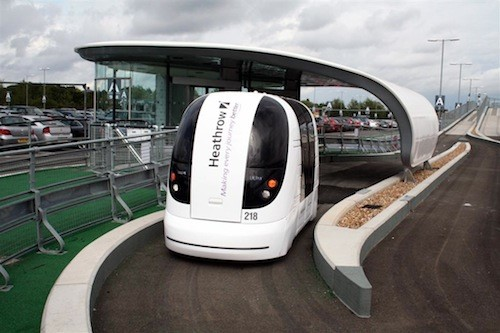
\includegraphics[width=0.4\linewidth]{image/PRT} \caption{PRT-Shuttle am Londoner Flughafen Heathrow (Kraft, 2012)}\label{fig:unnamed-chunk-45}
\end{figure}

Die Gründe für dieses begrenzte Auftreten sind die geringen technischen Möglichkeiten und die Skalierbarkeit von PRT-Systemen sowie die hohen Kapital- und Betriebskosten (Furman et al., 2014, S. 36).

\hypertarget{relevante-initiativen-in-uxf6sterreich-50}{%
\subsection*{Relevante Initiativen in Österreich}\label{relevante-initiativen-in-uxf6sterreich-50}}
\addcontentsline{toc}{subsection}{Relevante Initiativen in Österreich}

\begin{itemize}
\tightlist
\item
  \href{https://waset.org/personal-rapid-transit-and-system-design-conference-in-june-2023-in-vienna}{17th International Conference on Personal Rapid Transit and System Design in 2023}
\end{itemize}

\hypertarget{auswirkungen-in-bezug-auf-die-ziele-fuxfcr-nachhaltige-entwicklung-sdgs-50}{%
\subsection*{Auswirkungen in Bezug auf die Ziele für nachhaltige Entwicklung (SDGs)}\label{auswirkungen-in-bezug-auf-die-ziele-fuxfcr-nachhaltige-entwicklung-sdgs-50}}
\addcontentsline{toc}{subsection}{Auswirkungen in Bezug auf die Ziele für nachhaltige Entwicklung (SDGs)}

\begin{longtable}[]{@{}ccccc@{}}
\toprule
\begin{minipage}[b]{0.17\columnwidth}\centering
Ebene der Auswirkungen\strut
\end{minipage} & \begin{minipage}[b]{0.16\columnwidth}\centering
Indikator\strut
\end{minipage} & \begin{minipage}[b]{0.17\columnwidth}\centering
Richtung der Auswirkungen\strut
\end{minipage} & \begin{minipage}[b]{0.17\columnwidth}\centering
Beschreibung des Ziels \& SDG\strut
\end{minipage} & \begin{minipage}[b]{0.17\columnwidth}\centering
Quelle\strut
\end{minipage}\tabularnewline
\midrule
\endhead
\begin{minipage}[t]{0.17\columnwidth}\centering
Individuell\strut
\end{minipage} & \begin{minipage}[t]{0.16\columnwidth}\centering
Beeintraechtigung des visuellen Aspekts des staedtischen Raums\strut
\end{minipage} & \begin{minipage}[t]{0.17\columnwidth}\centering
\textbf{-}\strut
\end{minipage} & \begin{minipage}[t]{0.17\columnwidth}\centering
Gesundheit und Wohlbefinden (\emph{3})\strut
\end{minipage} & \begin{minipage}[t]{0.17\columnwidth}\centering
Staniscia, 2018\strut
\end{minipage}\tabularnewline
\begin{minipage}[t]{0.17\columnwidth}\centering
Systemisch\strut
\end{minipage} & \begin{minipage}[t]{0.16\columnwidth}\centering
Hoehenunterschiede erhoehen die Sicherheit\strut
\end{minipage} & \begin{minipage}[t]{0.17\columnwidth}\centering
\textbf{+}\strut
\end{minipage} & \begin{minipage}[t]{0.17\columnwidth}\centering
Gesundheit und Wohlbefinden (\emph{3})\strut
\end{minipage} & \begin{minipage}[t]{0.17\columnwidth}\centering
Juster \& Schonfeld, 2013; Furman et al., 2014\strut
\end{minipage}\tabularnewline
\begin{minipage}[t]{0.17\columnwidth}\centering
Systemisch\strut
\end{minipage} & \begin{minipage}[t]{0.16\columnwidth}\centering
Verwendet elektrische Energie\strut
\end{minipage} & \begin{minipage}[t]{0.17\columnwidth}\centering
\textbf{+}\strut
\end{minipage} & \begin{minipage}[t]{0.17\columnwidth}\centering
Oekologische Nachhaltigkeit (\emph{7,12,13,15})\strut
\end{minipage} & \begin{minipage}[t]{0.17\columnwidth}\centering
Juster \& Schonfeld, 2013\strut
\end{minipage}\tabularnewline
\begin{minipage}[t]{0.17\columnwidth}\centering
Systemisch\strut
\end{minipage} & \begin{minipage}[t]{0.16\columnwidth}\centering
Begrenzte Einfuehrung weltweit\strut
\end{minipage} & \begin{minipage}[t]{0.17\columnwidth}\centering
\textbf{-}\strut
\end{minipage} & \begin{minipage}[t]{0.17\columnwidth}\centering
Innovation und Infrastruktur (\emph{9})\strut
\end{minipage} & \begin{minipage}[t]{0.17\columnwidth}\centering
Furman et al., 2014\strut
\end{minipage}\tabularnewline
\bottomrule
\end{longtable}

\hypertarget{technologie--und-gesellschaftlicher-bereitschaftsgrad-46}{%
\subsection*{Technologie- und gesellschaftlicher Bereitschaftsgrad}\label{technologie--und-gesellschaftlicher-bereitschaftsgrad-46}}
\addcontentsline{toc}{subsection}{Technologie- und gesellschaftlicher Bereitschaftsgrad}

\begin{longtable}[]{@{}cc@{}}
\toprule
Stand der Technologiebereitschaft & Gesellschaftlicher Bereitschaftsgrad\tabularnewline
\midrule
\endhead
5-8 & 5-7\tabularnewline
\bottomrule
\end{longtable}

\hypertarget{offene-fragen-48}{%
\subsection*{Offene Fragen}\label{offene-fragen-48}}
\addcontentsline{toc}{subsection}{Offene Fragen}

\begin{enumerate}
\def\labelenumi{\arabic{enumi}.}
\tightlist
\item
  Es sind weitere Untersuchungen zur tatsächlichen Analyse von Kosten und Nutzen im Zusammenhang mit dem Bau von PRT erforderlich.
\item
  Kann die PRT-Infrastruktur als attraktives Stadtmobiliar betrachtet und genutzt werden? Wie kann die Kunstgemeinde in die Entwicklung einbezogen werden?
\item
  Was sind die Haupthindernisse für eine breitere Einführung von PRT?
\end{enumerate}

\hypertarget{weitere-links-41}{%
\subsection*{Weitere links}\label{weitere-links-41}}
\addcontentsline{toc}{subsection}{Weitere links}

\begin{itemize}
\tightlist
\item
  \href{https://transweb.sjsu.edu/sites/default/files/1227-automated-transit-networks.pdf}{MIT Report}
\end{itemize}

\hypertarget{referenzen-50}{%
\subsection*{Referenzen}\label{referenzen-50}}
\addcontentsline{toc}{subsection}{Referenzen}

\begin{itemize}
\tightlist
\item
  Furman, B., Fabian, L., Ellis, S., Muller, P., \& Swenson, R. (2014). Automated transit networks (ATN): A review of the state of the industry and prospects for the future.
\item
  Juster, R., \& Schonfeld, P. (2013). Comparative analysis of personal rapid transit as an urban transportation mode. Transportation research record, 2350(1), 128-135.
\item
  Kraft, A. (2012). The beginning of personal rapid transit. Available at: \url{https://www.zdnet.com/article/the-beginning-of-personal-rapid-transit/} {[}Accessed: 21 Oct 2021{]}
\item
  Mobolaji, K., Földes, D., \& Csiszár, C. (2021). Concept of Advanced Personal Rapid Transit at Airports. Periodica Polytechnica Civil Engineering, 65(1), 320-334.
\item
  Staniscia, S. (2018). Aesthetic appreciation of Personal Rapid Transit: A new viewpoint. Cities, 79, 169-177.
\end{itemize}

\hypertarget{brt}{%
\section{Busschnellverkehr (BRT - Bus rapid transit)}\label{brt}}

\hypertarget{synonyme-44}{%
\subsection*{Synonyme}\label{synonyme-44}}
\addcontentsline{toc}{subsection}{Synonyme}

\emph{Bus rapid transit (BRT), High-level bus transport (HLBT)}

\hypertarget{definition-51}{%
\subsection*{Definition}\label{definition-51}}
\addcontentsline{toc}{subsection}{Definition}

Städte auf der ganzen Welt sind bestrebt, die Kapazität ihres öffentlichen Verkehrssystems unter Berücksichtigung von Budgetbeschränkungen zu erweitern (Ishaq \& Cats, 2020). Bus-Rapid-Transit-Systeme (BRT) werden zunehmend als Alternativen für die Gestaltung des öffentlichen Massenverkehrs in mittelgroßen Städten in entwickelten Ländern in Betracht gezogen, um Verkehrsstaus mit ihren schädlichen Auswirkungen auf die öffentliche Gesundheit, die Wirtschaft und die Umwelt zu reduzieren. Bus Rapid Transit (BRT)-Systeme sind hochwertige busbasierte Verkehrssysteme, die einen schnellen und effizienten Service bieten (Abbasi et al., 2020). Erreicht wird dies durch die Bereitstellung eigener Fahrspuren, wobei die Busspuren und Haltestellen in der Regel auf die Straßenmitte ausgerichtet sind, durch die Möglichkeit der Fahrpreiserhebung außerhalb des Fahrzeugs sowie durch einen schnellen und häufigen Betrieb. Da BRT ähnliche Merkmale wie ein \protect\hyperlink{lrt}{Stadtbahn} - oder U-Bahnsystem aufweist, ist es viel zuverlässiger, bequemer und schneller als ein regulärer Busdienst. Mit den richtigen Merkmalen ist BRT in der Lage, die Ursachen für Verspätungen zu vermeiden, die den regulären Busverkehr in der Regel verlangsamen, wie z. B. im Verkehr stecken zu bleiben und in der Warteschlange zu stehen, um an Bord zu bezahlen (ITDP, 2021b).

Der Begriff Bus Rapid Transit (BRT) hat seinen Ursprung in Nordamerika und wird zunehmend auch in anderen Ländern verwendet. Dasselbe Konzept wird an verschiedenen Orten mit unterschiedlichen Namen bezeichnet (Deng \& Nelson, 2010):

\begin{itemize}
\tightlist
\item
  Hochkapazitäts-Bussysteme
\item
  Hochwertige Bussysteme
\item
  Metro-Bus
\item
  Oberflächen-Metro
\item
  Schnellbussysteme
\item
  Busstraßen-Systeme
\item
  Hochwertiger Busverkehr
  BRT-Systeme bieten eine leistungsfähige Alternative zu schienengebundenen Systemen, die wesentlich höhere Investitionen und eine längere Umsetzungszeit erfordern (Deng \& Nelson, 2010; Fageda, 2021). In großen Städten in Schwellenländern, insbesondere in Lateinamerika und Südasien, ist BRT ein integraler Bestandteil des öffentlichen Nahverkehrsnetzes oder bildet den Hauptteil davon. Im Gegensatz dazu ist die Einführung von BRT in den entwickelten Volkswirtschaften hauptsächlich auf mittelgroße Städte beschränkt, in denen die Nachfrage keine großen Investitionen in die städtische Schieneninfrastruktur rechtfertigt. Im europäischen Kontext werden diese Projekte manchmal als Busse mit hohem Verkehrsaufkommen (BHLS) bezeichnet (Ishaq \& Cats, 2020).
\end{itemize}

\textbf{BRT-Grundlagen}
Es gibt fünf wesentliche Merkmale, die BRT ausmachen. Diese Merkmale führen in erster Linie zu einer schnelleren Reise für die Fahrgäste und machen den Nahverkehr zuverlässiger und bequemer (ITDP, 2021b). Diese sind:

\begin{itemize}
\tightlist
\item
  Gewidmete Vorfahrt: Ausschließlich für Busse reservierte Fahrspuren sorgen für eine schnellere Fahrt und stellen sicher, dass die Busse nicht durch Staus im Mischverkehr aufgehalten werden.
\item
  Ausrichtung der Busspur: Entweder in der Mitte der Fahrbahn oder als reiner Buskorridor hält Busse von belebten Straßenrändern fern, an denen Autos parken, stehen und wenden.
\item
  Fahrpreiserhebung außerhalb des Busses: Durch die Bezahlung des Fahrpreises an der Haltestelle und nicht im Bus werden Verzögerungen durch wartende Fahrgäste im Bus vermieden.
\item
  Behandlung von Kreuzungen: Durch das Verbot des Abbiegens über die Busspur werden die durch den abbiegenden Verkehr verursachten Verspätungen des Busses verringert. Das Verbot solcher Abbiegevorgänge ist die wichtigste Maßnahme, um Busse durch Kreuzungen zu bewegen - sogar wichtiger als \protect\hyperlink{public_trans_priority}{Signalpriorität}.
\item
  Ebenerdiges Einsteigen: Die Bushaltestelle sollte in Höhe des Busses liegen, damit ein schneller und einfacher Einstieg möglich ist. Dadurch wird sie für Rollstuhlfahrer:innen, Behinderte, Kinderwagen und Fußgänger:innen mit minimalen Verzögerungen zugänglich.
\end{itemize}

Um als BRT zu gelten, muss ein Korridor (ITDP, 2021b, 2021a):

\begin{itemize}
\tightlist
\item
  Mindestens 3 km lang sein;
\item
  4 oder mehr Punkte im Element ``Gewidmetes Wegerecht'' erhalten;

  \begin{itemize}
  \tightlist
  \item
    8 Punkte: Physisch getrennte, eigene Fahrspuren (z. B. Zäune, Bordsteine, Bushaltestellen)
  \item
    6 Punkte: Farblich getrennte, eigene Fahrspuren ohne physische Trennung
  \item
    4 Punkte: Durch eine aufgemalte Linie abgetrennte getrennte Fahrspuren
  \item
    0 Punkte: Keine separaten Fahrspuren
  \end{itemize}
\item
  Mindestens 4 oder mehr Punkte beim Element Busausrichtung erhalten;

  \begin{itemize}
  \tightlist
  \item
    8 Punkte: Zwei-Wege-Busspur mit Mittelstreifen auf dem Mittelstreifen einer zweispurigen Straße
  \item
    8 Punkte: Ausschließlicher Buskorridor mit ausschließlicher Vorfahrt und ohne parallelen Mischverkehr oder umgewandelten Korridor
  \item
    8 Punkte: Busstraße, die entlang einer Randbedingung wie einer Uferpromenade oder einem Park verläuft, wo es nur wenige Kreuzungen gibt, die Konflikte verursachen
  \end{itemize}
\item
  Mindestens 20 oder mehr Punkte in allen fünf grundlegenden BRT-Elementen erhalten

  \begin{itemize}
  \tightlist
  \item
    Gewidmetes Wegerecht (bis zu 8 Punkte)

    \begin{itemize}
    \tightlist
    \item
      Bewährtes Verfahren: Der Rainbow BRT-Korridor Sangamwadi-Vishrantwadi (Pune/Pimpri-Chinchwad, Indien), bei dem Zäune zur Schaffung eigener, räumlich getrennter Busspuren verwendet werden.
    \end{itemize}
  \item
    Ausrichtung der Busspuren (bis zu 8 Punkte)

    \begin{itemize}
    \tightlist
    \item
      Bewährtes Verfahren: Die Metrobus Green Line (Lahore, Pakistan), die eine in beide Richtungen ausgerichtete Busspur in der Mitte einer Fahrbahn umfasst.
    \end{itemize}
  \item
    Fahrgeldeinzug außerhalb des Fahrzeugs (bis zu 8 Punkte)

    \begin{itemize}
    \tightlist
    \item
      Bewährtes Verfahren: Der TransJakarta Koridor 1 (Jakarta, Indonesien) bietet einen fahrerlosen Fahrscheinverkauf mit Zugang zu den Stationen über Drehkreuze.
    \end{itemize}
  \item
    Behandlung von Kreuzungen (bis zu 7 Punkte)

    \begin{itemize}
    \tightlist
    \item
      Bewährtes Verfahren: Corredor Metropolitano ABD (São Paulo, Brasilien), der Fußgänger:innen Vorrang einräumt und das Linksabbiegen an Kreuzungen verbietet.
    \end{itemize}
  \item
    Einsteigen auf Bahnsteigebene (bis zu 7 Punkte)

    \begin{itemize}
    \tightlist
    \item
      Bewährtes Verfahren: Ahmedabad BRTS (Ahmedabad, Indien), das durch eine gut durchdachte Infrastruktur und Fahrerschulung den Einstiegsabstand auf weniger als 10 Zentimeter reduzieren konnte.
    \end{itemize}
  \end{itemize}
\end{itemize}

Weitere Informationen zum Punktesystem finden Sie unter \href{https://www.itdp.org/library/standards-and-guides/the-bus-rapid-transit-standard/the-scorecard/}{scorecard}.

\textbf{Offen vs.~geschlossen}
BRT kombiniert Bahnhöfe, Fahrzeuge und Technologie zu einem hochwertigen, schienenähnlichen System und kann zur Verbesserung der städtischen Mobilität beitragen. Das Wiederaufleben des Busverkehrs in den letzten Jahren ist bei Verkehrs- und Stadtplaner:innen auf großes Interesse gestoßen, da er flexible, hochwertige Dienstleistungen zu geringeren Kosten als ein schienengebundenes Verkehrssystem bietet. Angesichts vieler erfolgreicher Systeme in der ganzen Welt sind die Investitionen in BRT in die Höhe geschnellt. Einer der Vorteile von BRT ist die Flexibilität bei der Gestaltung von Korridoren und Stationen. BRT kann mit Bussen unter verschiedenen Verkehrsbedingungen betrieben werden, z. B. im Mischverkehr, auf eigenen Fahrspuren auf Landstraßen und auf Busways (Autobahnen oder Fahrspuren einer Autobahn, die ausschließlich für BRT reserviert sind). In Nordamerika nutzen die meisten BRT-Systeme separate oder getrennte Fahrspuren, während in Südamerika BRT-Systeme die mittleren Fahrspuren nutzen. Ein weiterer Vorteil von BRT ist die betriebliche Flexibilität bei der Integration mit bestehenden konventionellen Buslinien.

BRT kann entweder als offenes oder geschlossenes System betrieben werden. Ein geschlossenes System bedeutet, dass BRT-Busse nur auf dem BRT-Korridor verkehren können und Nicht-BRT-Busse nicht auf dem BRT-Korridor fahren können (Zhang et al., 2020b). Die Nutzer:innen betrachten ein geschlossenes BRT-System in der Regel als einen häufigen und pünktlichen schienenähnlichen Dienst, der die meisten der typischen Verspätungsursachen beseitigt, die bei herkömmlichen Busdiensten auftreten (Zhang et al., 2020a). Einige neuere BRT-Systeme (Seoul in Südkorea, Guangzhou in China und Sydney, Adelaide und Brisbane in Australien) haben einen offenen Systemansatz gewählt, bei dem konventionelle Busse in den BRT-Korridor ein- und ausfahren. Diese offenen BRT-Dienste ermöglichen es den Fahrgästen, den BRT-Korridor zu erreichen, ohne den Bus wechseln zu müssen. In einem offenen BRT-System können sie die BRT-Zugänglichkeit für Fahrgäste abseits des BRT-Korridors wirksam verbessern, indem sie die mit dem Umsteigen verbundenen Nachteile sowie die zusätzliche Geh- und Wartezeit beseitigen (Yen et al., 2018). Allerdings können diese Zubringerdienste, die den BRT-Korridor für einen Teil ihrer Strecken nutzen, vom lokalen Verkehr betroffen sein, was die Gesamtleistung des BRT-Dienstes verringert. Da busbasierte Systeme jedoch flexibel sind, könnte manchmal auch eine hybride Betriebsart geeignet sein. Verkehrsplaner:innen können die Buslinien überprüfen, um Strecken mit hohem Fahrgastaufkommen zu ermitteln und auf diesen Strecken ein offenes BRT-System zu betreiben, während auf anderen Strecken mit geringem Fahrgastaufkommen zusätzliche Dienste als geschlossenes System betrieben werden und ein Netz von Zubringerbussen für diese Dienste eingerichtet wird. Dieses Konzept kann auf verschiedene Tageszeiten angewandt werden, wobei der BRT-Korridor außerhalb der Hauptverkehrszeiten ein offenes System ist, um Einzelfahrten zu ermöglichen, und während der Hauptverkehrszeiten geschlossen ist, um Überbelegung und Staus zu vermeiden (Zhang et al., 2020b).

\hypertarget{wichtige-interessensgruppen-51}{%
\subsection*{Wichtige Interessensgruppen}\label{wichtige-interessensgruppen-51}}
\addcontentsline{toc}{subsection}{Wichtige Interessensgruppen}

\begin{itemize}
\tightlist
\item
  \textbf{Betroffene}: Mobile Bürger:innen, Nutzer:innen öffentlicher Verkehrsmittel
\item
  \textbf{Verantwortliche}: Nationale Regierungen, Stadtverwaltungen, Privatunternehmen, Verkehrsbetriebe, Infrastrukturanbieter, Bushersteller
\end{itemize}

\hypertarget{aktueller-stand-der-wissenschaft-und-forschung-51}{%
\subsection*{Aktueller Stand der Wissenschaft und Forschung}\label{aktueller-stand-der-wissenschaft-und-forschung-51}}
\addcontentsline{toc}{subsection}{Aktueller Stand der Wissenschaft und Forschung}

Viele Forscher:innen konzentrieren sich auf lokale BRT-Systeme mit unterschiedlichen Schwerpunkten wie Malik et al.~(2021) untersucht das Reiseverhalten der Nutzer:innen in Lahore, Kiani. Mavi et al.~(2018) evaluiert und optimiert eine BRT-Linie in Teheran (Iran) mit Hilfe eines Simulations- und multikriteriellen Entscheidungsfindungsansatzes. Ishaq \& Cats (2020) berichten über empirische Erkenntnisse aus der Umsetzung eines BRT-Systems in Haifa (Israel). Mallqui \& Pojani (2017) schließlich vergleichen Fragen des Bus Rapid Transit (BRT) in Brisbane (Australien) mit Lima (Peru). In beiden Städten hat eine Bürgerbeteiligung stattgefunden. Ungeachtet der Konkurrenz durch andere Verkehrsträger wurden beide BRT-Systeme von der lokalen Bevölkerung positiv aufgenommen. Insbesondere die Menschen, die in der Nähe der Bahnhöfe wohnen und die BRTs für ihren Arbeitsweg nutzen können, stehen diesem Verkehrsmittel sehr positiv gegenüber.
Schwanen \& Ferbrache (2017) von der Transport Studies Unit an der University of Oxford haben eine Liste mit Literatur zu den weiteren wirtschaftlichen und sozialen Auswirkungen von Bus Rapid Transit (BRT) zusammengestellt. Die folgenden Themen werden in der Literatur behandelt:

\begin{itemize}
\tightlist
\item
  BRT-Folgestudien, die die weitergehenden wirtschaftlichen und sozialen Auswirkungen von BRT untersuchen.
\item
  Landentwicklung, Landnutzungsänderung und/oder verkehrsorientierte Entwicklung.
\item
  Veränderung der Boden-/Grundstückswerte
\item
  neue wirtschaftliche Entwicklung
\item
  Zugänglichkeit von Arbeitsplätzen/Arbeitsplätzen
\item
  Verbesserung der städtischen Umwelt
\item
  Prestige/Reputation der Stadt
\item
  physische Verdrängung ärmerer Haushalte
\end{itemize}

Mehrere Forscher:innen haben die Auswirkungen von Bus Rapid Transit (BRT) auf Immobilienwerte untersucht (Zhang et al., 2020a; Zhang \& Yen, 2020)). Zhang \& Yen (2020) verglichen 23 andere Studien zu diesem Thema und kamen zu folgenden zwei Hauptschlussfolgerungen:

\begin{itemize}
\tightlist
\item
  Der geschätzte Wertzuwachs für Grundstücke ist viel höher als für Immobilien (d.~h. 27,5 \% höher).
\item
  Im Allgemeinen haben Grundstücke und Immobilien im Umkreis von 50 m von einer BRT-Station einen Preisaufschlag von 13,0 \% gegenüber Grundstücken und Immobilien in 1,2 km Entfernung.
\end{itemize}

Diese Ergebnisse können zu einem besseren Verständnis der Erreichbarkeitsvorteile von BRT-Systemen beitragen, insbesondere dort, wo es an empirischen Belegen mangelt. Allerdings fehlt es an Belegen für europäische BRT-Systeme, und nur wenige Studien haben untersucht, wie BRT-Systeme die Grundstücks- und Immobilienwerte im Laufe der Zeit beeinflussen.

Basso et al.~(2019) schlugen einen dynamischen Stauansatz vor, der Warteschlangen sowohl auf der Straße als auch an BRT-Stationen endogen modelliert. Einige der wichtigsten Ergebnisse sind:

\begin{itemize}
\tightlist
\item
  Das optimale BRT ist in Bezug auf die Gesamtkosten effizient, und selbst bei unvollkommen teilbarer Kapazität ist BRT für viele Nachfrageniveaus immer noch die bessere Wahl (beginnend mit einer Nachfrage zwischen 8000 und 8500 Pendler:innen).
\item
  Ohne BRT gibt es ein großes Nachfrageschnittintervall, in dem es optimal ist, keinen öffentlichen Verkehr anzubieten (bis zu 10.000 Pendler:innen). Wenn jedoch ein Teil der Straßenkapazität ausschließlich für Busse reserviert wäre, müssten die Busse im Optimalfall sehr häufig fahren. Stadtplaner:innen sollten daher BRT-Systeme von Anfang an planen, anstatt den öffentlichen Verkehr schrittweise zu integrieren, bis die Nachfrage so groß wird, dass es zu Verkehrsüberlastungen kommt. Folglich die Busfrequenzen häufiger werden und dedizierte Busspuren notwendig werden.
\item
  Die Betriebszeiten von Bussen und Autos sind bei BRT viel kürzer als bei Mischverkehr. Obwohl BRT dem Pkw-Verkehr Kapazitäten entzieht, wird die Spitzenzeit des Pkw-Verkehrs reduziert.
\end{itemize}

Abbasi et al.~(2020) haben verschiedene Aspekte von BRT in Teheran (Iran) untersucht. In ihren Simulationen hatten exklusive Busspuren gute Auswirkungen auf die Reduzierung der Schadstoffemissionen und des Kraftstoffverbrauchs. Im Durchschnitt würden die Szenarien mit exklusiven Busspuren die CO-Emissionen von Bussen um 40,6 \% reduzieren und die CO-Emissionen von Pkw um 3,1 \% erhöhen, ebenso wie die NOx-Emissionen (Busse um 15,1 \% reduziert, Pkw um 6,7 \% erhöht), die PM-Emissionen (Busse um 6,7 \% reduziert, Pkw um 4,4 \% erhöht) und den Kraftstoffverbrauch (Busse um 5,6 \% reduziert, Pkw um 3,2 \% erhöht). In den Szenarien der effizienten Nutzung und der Vereinheitlichung der Anzahl der Stationen werden nicht nur die Schadstoffemissionen der Busse, sondern auch die der Pkw reduziert. Ein möglicher Grund dafür ist die Verringerung von Konflikten zwischen Bussen und Pkw auf gemeinsamen Fahrspuren. Im Szenario mit geschalteten Ampeln und Busvorrang sinken die Schadstoffemissionen und der Kraftstoffverbrauch der Busse im Durchschnitt um 10,2 \%, während sie bei den Pkw um 1,3 \% steigen. Aus wirtschaftlicher Sicht wurden die jährlichen Kosten bei der vollständigen exklusiven Busspur am stärksten reduziert.

\hypertarget{aktueller-stand-der-praktischen-umsetzung-51}{%
\subsection*{Aktueller Stand der praktischen Umsetzung}\label{aktueller-stand-der-praktischen-umsetzung-51}}
\addcontentsline{toc}{subsection}{Aktueller Stand der praktischen Umsetzung}

BRT-Systeme gediehen zunächst in lateinamerikanischen Städten (Dario Hidalgo \& Graftieaux, 2008), bevor sie sich in Süd- und Ostasien und dann in der ganzen Welt ausbreiteten (Darío Hidalgo \& Gutiérrez, 2013). Doch obwohl die Zahl der BRT-Systeme weltweit zunimmt, befinden sich derzeit nur \textasciitilde10 \% der BRT-Systeme in Ländern mit niedrigem und mittlerem Einkommen (Malik et al., 2021).

Laut (Global BRTData, 2021) ist die Verteilung der BRT-Systeme weltweit (Stand 2021) in Bezug auf die Fahrgastzahlen (weltweit täglich 33.684.575) aufgeteilt in Afrika mit 491.578 Fahrgästen (1. 45\%), Asien 9.238.060 (27,42\%), Europa 1.613.580 (4,79\%), Lateinamerika 20.916.474 (62,09\%), Nordamerika 988.683 (2,93\%) und Ozeanien 436.200 (1,29\%).

Drei neue BRT-Systeme in Australien (Busway in Adelaide, Brisbane und Sydney) sind offene Systeme. Dies könnte auf die Merkmale der australischen Stadtgebiete zurückzuführen sein, die in der Regel eine geringe Bevölkerungsdichte und eine hohe Autonutzung aufweisen. Da die Fahrgäste umsteigen müssen, ist es für ein geschlossenes System schwieriger, die Vorteile des Netzeffekts zu nutzen, und ein offenes BRT-System könnte in diesem vom Auto dominierten Umfeld attraktiver sein. In Brisbane wird jedoch erwogen, auf ein geschlossenes BRT-Betriebssystem umzusteigen, da es vor allem zu den Stoßzeiten zu erheblichen Verkehrsstaus kommt (Zhang et al., 2020b).

Laut Daimler erkennen immer mehr Europäer die Vorteile effektiver und attraktiver städtischer Busverkehrssysteme. Als Vorreiter wird Frankreich genannt, wo die Regierung den Ausbau von BRT-Systemen mit hohen Summen unterstützt (Daimler (EvoBus GmbH), n.d.). Dies wird durch das weltweit erste wasserstoffbetriebene Schnellbussystem umgesetzt, das unter dem Namen Fébus in der französischen Stadt Pau in Betrieb genommen wurde. Zum Einsatz kommen acht ExquiCity18-Brennstoffzellen-Van-Hool-Busse in Stadtbahnbauweise. Die 18 Meter langen Gelenkbusse bieten Platz für 125 Fahrgäste und können mehr als 300 Kilometer pro Wasserstofffüllung zurücklegen (Schaal, 2019).

Darüber hinaus werden zwei BRT-Linien für das öffentliche Verkehrssystem in Florenz eingeführt. Die beiden Linien werden das Netz des öffentlichen Verkehrs auf der Straße vervollständigen, um die Busse zu entlasten, die derzeit auf diesen Strecken verkehren. Diese Innovation wird durch den Metrocittà-Plan für nachhaltige Mobilität ermöglicht (autobusweb.com, 2021).

In Istanbul erstreckt sich das BRT-Netzwerk bereits über insgesamt 52 Kilometer und befördert täglich 750.000 Fahrgäste. Städte wie Amsterdam, Straßburg und Paris betreiben bereits ihr eigenes BRT-System. In Deutschland wurde das BRT-System noch nicht eingeführt, da die Bahn immer noch die erste Wahl ist. Laut Richard Mejía (Leiter des BRT-Teams bei Daimler Buses) sind die Investitions- und Betriebskosten im Vergleich zu Schienensystemen geringer. Zur zukünftigen Entwicklung von BRT wird erwähnt, dass das bisherige Konzept ständig weiterentwickelt und an neue Technologien oder aktuelle Stadtplanungen angepasst wird. Derzeit werden die Weichen für emissionsfreies Fahren mit Elektromobilität gestellt. Auch das teilautomatisierte Fahren von Bussen (z.B. der Future Bus von Mercedes-Benz, der Mitte 2016 vorgestellt wurde) könnte durch ein konstantes Beschleunigungs- und Bremsverhalten den Kraftstoffverbrauch senken. Auch eine erweiterte und intelligente Vernetzung, zum Beispiel zwischen Fahrzeugen, Signalanlagen und Fahrbahn, wird BRT-Systeme in Zukunft noch attraktiver machen (Daimler AG, n.d.).

\hypertarget{relevante-initiativen-in-uxf6sterreich-51}{%
\subsection*{Relevante Initiativen in Österreich}\label{relevante-initiativen-in-uxf6sterreich-51}}
\addcontentsline{toc}{subsection}{Relevante Initiativen in Österreich}

Kärnten könnte ein Schnellbussystem für den Nahverkehr bekommen.

\begin{itemize}
\tightlist
\item
  \href{https://kaernten.orf.at/stories/3029225/}{Kaernten.orf.at}
\end{itemize}

Derzeit verbinden elf Schnellbuslinien, das so genannte Schnellbussystem (ohne eigene Fahrspuren), die Zentren der 3 umliegenden Bezirke mit der Landeshauptstadt St.~Pölten. Der Fuhrpark besteht aus 47 Fahrzeugen in vier verschiedenen Größen im einheitlichen Wiesel-Design, die zusammen eine Sitzplatzkapazität für 2.449 Fahrgäste bieten.

\begin{itemize}
\tightlist
\item
  \href{https://www.meinbezirk.at/st-poelten/c-lokales/wieselbus-erfolgsstory-feiert-20-jahre_a1863287}{Meinbezirk.at}
\end{itemize}

\hypertarget{auswirkungen-in-bezug-auf-die-ziele-fuxfcr-nachhaltige-entwicklung-sdgs-51}{%
\subsection*{Auswirkungen in Bezug auf die Ziele für nachhaltige Entwicklung (SDGs)}\label{auswirkungen-in-bezug-auf-die-ziele-fuxfcr-nachhaltige-entwicklung-sdgs-51}}
\addcontentsline{toc}{subsection}{Auswirkungen in Bezug auf die Ziele für nachhaltige Entwicklung (SDGs)}

\begin{longtable}[]{@{}ccccc@{}}
\toprule
\begin{minipage}[b]{0.17\columnwidth}\centering
Ebene der Auswirkungen\strut
\end{minipage} & \begin{minipage}[b]{0.16\columnwidth}\centering
Indikator\strut
\end{minipage} & \begin{minipage}[b]{0.17\columnwidth}\centering
Richtung der Auswirkungen\strut
\end{minipage} & \begin{minipage}[b]{0.17\columnwidth}\centering
Beschreibung des Ziels \& SDG\strut
\end{minipage} & \begin{minipage}[b]{0.17\columnwidth}\centering
Quelle\strut
\end{minipage}\tabularnewline
\midrule
\endhead
\begin{minipage}[t]{0.17\columnwidth}\centering
Systemisch\strut
\end{minipage} & \begin{minipage}[t]{0.16\columnwidth}\centering
Verringerung der Schadstoffemissionen und des Kraftstoffverbrauchs\strut
\end{minipage} & \begin{minipage}[t]{0.17\columnwidth}\centering
\textbf{+}\strut
\end{minipage} & \begin{minipage}[t]{0.17\columnwidth}\centering
Oekologische Nachhaltigkeit (\emph{7,12,13,15})\strut
\end{minipage} & \begin{minipage}[t]{0.17\columnwidth}\centering
Abbasi et al., 2020\strut
\end{minipage}\tabularnewline
\begin{minipage}[t]{0.17\columnwidth}\centering
Systemisch\strut
\end{minipage} & \begin{minipage}[t]{0.16\columnwidth}\centering
BRT erfordert wesentlich kuerzere Investitionen und Umsetzungszeiten\strut
\end{minipage} & \begin{minipage}[t]{0.17\columnwidth}\centering
\textbf{+}\strut
\end{minipage} & \begin{minipage}[t]{0.17\columnwidth}\centering
Innovation und Infrastruktur (\emph{9})\strut
\end{minipage} & \begin{minipage}[t]{0.17\columnwidth}\centering
Deng \& Nelson, 2010; Fageda, 2021\strut
\end{minipage}\tabularnewline
\bottomrule
\end{longtable}

\hypertarget{technologie--und-gesellschaftlicher-bereitschaftsgrad-47}{%
\subsection*{Technologie- und gesellschaftlicher Bereitschaftsgrad}\label{technologie--und-gesellschaftlicher-bereitschaftsgrad-47}}
\addcontentsline{toc}{subsection}{Technologie- und gesellschaftlicher Bereitschaftsgrad}

\begin{longtable}[]{@{}cc@{}}
\toprule
Stand der Technologiebereitschaft & Gesellschaftlicher Bereitschaftsgrad\tabularnewline
\midrule
\endhead
7-9 & 7-9\tabularnewline
\bottomrule
\end{longtable}

\hypertarget{offene-fragen-49}{%
\subsection*{Offene Fragen}\label{offene-fragen-49}}
\addcontentsline{toc}{subsection}{Offene Fragen}

\begin{enumerate}
\def\labelenumi{\arabic{enumi}.}
\tightlist
\item
  Wie kann die Entwicklung von BRT-Systemen durch die nationale Politik besser unterstützt werden?
\end{enumerate}

\hypertarget{weitere-links-42}{%
\subsection*{Weitere links}\label{weitere-links-42}}
\addcontentsline{toc}{subsection}{Weitere links}

\begin{itemize}
\tightlist
\item
  \href{http://brtdata.org/}{BRT data}
\item
  \href{https://www.itdp.org/library/standards-and-guides/the-bus-rapid-transit-standard/what-is-brt/}{What is BRT?}
\item
  \href{https://www.itdp.org/library/standards-and-guides/the-bus-rapid-transit-standard/the-scorecard/}{Scorecard}
\item
  \href{https://www.transit.dot.gov/sites/fta.dot.gov/files/issues.pdf}{BRT issues}
\end{itemize}

\hypertarget{referenzen-51}{%
\subsection*{Referenzen}\label{referenzen-51}}
\addcontentsline{toc}{subsection}{Referenzen}

\begin{itemize}
\tightlist
\item
  Abbasi, M. H., Hadji Hosseinlou, M., \& JafarzadehFadaki, S. M. (2020). An investigation of Bus Rapid Transit System (BRT) based on economic and air pollution analysis (Tehran, Iran). Case Studies on Transport Policy, 8(2), 553--563. \url{https://doi.org/10.1016/j.cstp.2019.11.008}
\item
  autobusweb.com. (2021, March 2). Trasporto pubblico Firenze, in arrivo due linee Bus Rapid Transit. \url{https://www.autobusweb.com/tpl-firenze-in-arrivo-due-linee-bus-rapid-transit/}
\item
  Basso, L. J., Feres, F., \& Silva, H. E. (2019). The efficiency of bus rapid transit (BRT) systems: A dynamic congestion approach. Transportation Research Part B: Methodological, 127, 47--71. \url{https://doi.org/10.1016/j.trb.2019.06.012}
\item
  Daimler (EvoBus GmbH). (n.d.). Bus Rapid Transit (BRT) in Europe -- Impressions of a sustainable mobility concept in Strasbourg - EvoBus GmbH. Available at: \url{https://www.evobus.com/de-en/layer/bus-rapid-transit-brt-in-europe-impressions-of-a-sustainable-mobility-concept-in-strasbourg/} {[}Accessed: 24 June 2021{]}
\item
  Daimler AG. (n.d.). Bus Rapid Transit -- Neue Unabhängigkeit im Stadtverkehr \textbar{} Daimler. Available at: \url{https://www.daimler.com/nachhaltigkeit/staedte/bus-rapid-transit.html} {[}Accessed: 24 June 2021{]}
\item
  Deng, T., \& Nelson, J. D. (2010). Transport Reviews Recent Developments in Bus Rapid Transit: A Review of the Literature. \url{https://doi.org/10.1080/01441647.2010.492455}
\item
  Fageda, X. (2021). Do light rail systems reduce traffic externalities? Empirical evidence from mid-size european cities. Transportation Research Part D: Transport and Environment, 92, 102731. \url{https://doi.org/10.1016/j.trd.2021.102731}
\item
  Global BRTData. (2021). Global BRTData. Brtdata.Org. \url{http://brtdata.org/}
\item
  Hidalgo, Dario, \& Graftieaux, P. (2008). Bus Rapid Transit Systems in Latin America and Asia: Results and Difficulties in 11 Cities. Transportation Research Record, 2072(1), 77--88. \url{https://doi.org/10.3141/2072-09}
\item
  Hidalgo, Darío, \& Gutiérrez, L. (2013). BRT and BHLS around the world: Explosive growth, large positive impacts and many issues outstanding. Research in Transportation Economics, 39(1), 8--13. \url{https://doi.org/10.1016/j.retrec.2012.05.018}
\item
  Ishaq, R., \& Cats, O. (2020). Designing bus rapid transit systems: Lessons on service reliability and operations. Case Studies on Transport Policy, 8(3), 946--953. \url{https://doi.org/10.1016/j.cstp.2020.05.001}
\item
  ITDP. (2021a). The Scorecard - Institute for Transportation and Development Policy. \url{https://www.itdp.org/library/standards-and-guides/the-bus-rapid-transit-standard/the-scorecard/}
\item
  ITDP. (2021b). What is BRT? - Institute for Transportation and Development Policy. \url{https://www.itdp.org/library/standards-and-guides/the-bus-rapid-transit-standard/what-is-brt/}
\item
  Kiani Mavi, R., Zarbakhshnia, N., \& Khazraei, A. (2018). Bus rapid transit (BRT): A simulation and multi criteria decision making (MCDM) approach. Transport Policy, 72, 187--197. \url{https://doi.org/10.1016/j.tranpol.2018.03.010}
\item
  Malik, B. Z., Rehman, Z. ur, Khan, A. H., \& Akram, W. (2021). Investigating users' travel behaviours and perceptions of single-corridor BRT: Lessons from Lahore. Journal of Transport Geography, 91, 102942. \url{https://doi.org/10.1016/j.jtrangeo.2020.102942}
\item
  Mallqui, Y. Y. C., \& Pojani, D. (2017). Barriers to successful Bus Rapid Transit expansion: Developed cities versus developing megacities. Case Studies on Transport Policy, 5(2), 254--266. \url{https://doi.org/10.1016/j.cstp.2017.01.004}
\item
  Schaal, S. (2019, December 18). Fébus: Erstes H2-Schnellbussystem in Betrieb - electrive.net. \url{https://www.electrive.net/2019/12/18/febus-erstes-h2-schnellbussystem-in-betrieb/}
\item
  Schwanen, T., \& Ferbrache, F. (2017). Bibliography of Research on Bus Rapid Transit. 1068. \url{https://www.tsu.ox.ac.uk/pubs/1068-schwanen-ferbrache.pdf}
\item
  Yen, B. T. H., Mulley, C., Tseng, W. C., \& Chiou, Y. C. (2018). Assessing interchange effects in public transport: A case study of South East Queensland, Australia. Case Studies on Transport Policy, 6(3), 364--375. \url{https://doi.org/10.1016/j.cstp.2018.01.005}
\item
  Zhang, M., \& Yen, B. T. H. (2020). The impact of Bus Rapid Transit (BRT) on land and property values: A meta-analysis. Land Use Policy, 96, 104684. \url{https://doi.org/10.1016/j.landusepol.2020.104684}
\item
  Zhang, M., Yen, B. T. H., Mulley, C., \& Sipe, N. (2020a). An investigation of the open-system Bus Rapid Transit (BRT) network and property values: The case of Brisbane, Australia. Transportation Research Part A: Policy and Practice, 134, 16--34. \url{https://doi.org/10.1016/j.tra.2020.01.021}
\item
  Zhang, M., Yen, B. T. H., Mulley, C., \& Sipe, N. (2020b). How does an open system bus rapid transit (BRT) facilitate inter and intra-modal mobility? A visual analytic analysis of Brisbane, Australia. Research in Transportation Economics, 83, 100906. \url{https://doi.org/10.1016/j.retrec.2020.100906}
\end{itemize}

\hypertarget{lrt}{%
\section{Stadtbahnverkehr (LRT - Light Rail Transit)}\label{lrt}}

\hypertarget{synonyme-45}{%
\subsection*{Synonyme}\label{synonyme-45}}
\addcontentsline{toc}{subsection}{Synonyme}

\emph{Light Rail Transit (LRT), Schnellbahn (HRT - Heavy Rail Transit)}

\hypertarget{definition-52}{%
\subsection*{Definition}\label{definition-52}}
\addcontentsline{toc}{subsection}{Definition}

Stadtbahnen (auch als Straßenbahn bezeichnet) sind bei Stadtplaner:innen zu einer beliebten Maßnahme geworden, um die mit dem städtischen Wachstum verbundenen sozialen und wirtschaftlichen Probleme anzugehen (Baker \& Lee, 2019). Stadtbahnentwicklungen gehen über die Verbesserung des Zugangs zu öffentlichen Verkehrsmitteln für die umliegenden Stadtteile hinaus. Die Auswirkungen können sich auch auf Immobilienwerte, die Demografie der Nachbarschaft, Beschäftigungsmöglichkeiten und den Zugang zu Dienstleistungen auswirken (Hess, 2020).

Befürworter:innen argumentieren, dass die Einrichtung neuer Stadtbahnlinien die ökologische Nachhaltigkeit fördern kann, indem sie die Nutzung des privaten Pkw reduziert und die öffentliche Gesundheit verbessert, indem sie die Begehbarkeit der Nachbarschaft und die Luftqualität erhöht (D. Knowles \& Ferbrache, 2016). Andere Argumente sind, dass LRTs die Einkommensungleichheit positiv beeinflussen, indem sie die Entwicklung von Unternehmen fördern und einen direkten Zugang zu Beschäftigungszentren in einer Stadt oder einem Vorort bieten (Hess, 2020).

Viele dieser Auswirkungen haben Auswirkungen auf die Gesundheit und das Wohlbefinden der Bewohner:innen. Diese werden anhand der sozialen Determinanten der Gesundheit (SDOH) bewertet. Die Weltgesundheitsorganisation (WHO) definiert die sozialen Determinanten der Gesundheit (SDOH) als ``\emph{die Bedingungen, unter denen Menschen geboren werden, aufwachsen, leben, arbeiten und altern}'' (z. B. Einkommen, Wohnen, Beschäftigung) und ``\emph{die diesen Bedingungen zugrunde liegenden Faktoren}'' (z. B. Wirtschafts- und Sozialpolitik und politische Systeme) (Braveman \& Gottlieb, 2014). Das SDOH-Rahmenwerk geht davon aus, dass die Art und Weise, wie politische, soziale und wirtschaftliche Ressourcen innerhalb von Gemeinschaften verteilt sind, Auswirkungen auf Gesundheit und Wohlbefinden haben kann (Solar \& Irwin, 2010).

Aufgrund der niedrigen Baukosten im Vergleich zu unterirdischen Systemen und der großen wahrgenommenen wirtschaftlichen Vorteile ist LRT zu einer beliebten Form des Transits geworden. LRT-Systeme werden in der Regel entlang bestehender Straßen gebaut, so dass keine teure Tunnel- oder Hochbahninfrastruktur erforderlich ist. LRT teilen sich zwar den Straßenraum mit Fahrzeugen und Fußgänger:innen, doch werden Teile der Strecken mit Vorrang befahren, was höhere Geschwindigkeiten und weniger Verspätungen als bei Bussen ermöglicht. Im Gegensatz zum Bustransit wird durch die Notwendigkeit von Schienen, einer oberirdischen Stromquelle und Bahnsteigen sichergestellt, dass LRT eine langfristige lokale Investition ist (Tyndall, 2021).

Laird (2019) definiert die Unterschiede zwischen Stadtbahnsystemen und Nahverkehrsbahnsystemen. Sie funktionieren unterschiedlich, haben unterschiedliche Anforderungen und verwenden unterschiedliche Systeme für den Betrieb:

\textbf{Nahverkehrsbahnsysteme (S-Bahnen)}
Nahverkehrsbahnen sind Personenzüge, die mit diesel-elektrischen oder elektrischen Motoren betrieben werden. Sie verkehren auf bestehenden Gleisanlagen auf denselben Strecken, die auch von Güterzügen im Fernverkehr genutzt werden. Sie werden von staatlichen Behörden oder privaten Unternehmen auf eigenen oder fremden Gleisen betrieben. Sie haben in der Regel eine Geschwindigkeit von 80 bis 130 km/h, kürzere Strecken und sind meist nur in größeren Ballungsräumen zu finden. Nahverkehrssysteme haben weniger Haltestellen als Stadtbahnen und verkehren in der Regel durch Vororte und zentrale Städte. Da S-Bahn-Systeme für Pendler:innen konzipiert sind, kann die Fahrplanhäufigkeit anders sein als bei der Stadtbahn und über den Tag verteilt weniger häufig verkehren. Die meisten Pendlerzüge verkehren während der üblichen Pendlerzeiten an einem durchschnittlichen Arbeitstag.

\textbf{Stadtbahnsysteme (Straßenbahnen)}
Stadtbahnsysteme sind Personenzüge, die durch elektrische Oberleitungen angetrieben werden. Sie haben leichtere Rahmen und kleinere Wagenkästen als andere Züge, da sie einen größeren Wendekreis benötigen. Da Stadtbahnen auf städtischen Straßen und in städtischen Korridoren mit häufigen Haltestellen verkehren, haben sie einen kleineren Wenderadius, um in verkehrsreiche Bereiche hinein- und wieder herauszufahren, und können schneller beschleunigen und abbremsen als Nahverkehrszüge. Während Nahverkehrsbahnsysteme über bestehende Güterzuggleise fahren können, benötigen Stadtbahnsysteme in der Regel eigene Gleise.

\hypertarget{wichtige-interessensgruppen-52}{%
\subsection*{Wichtige Interessensgruppen}\label{wichtige-interessensgruppen-52}}
\addcontentsline{toc}{subsection}{Wichtige Interessensgruppen}

\begin{itemize}
\tightlist
\item
  \textbf{Betroffene}: Fußgänger:innen, Benutzer:innen öffentlicher Verkehrsmittel, Anwohner:innen, Autofahrer:innen
\item
  \textbf{Verantwortliche}: Stadtverwaltungen, private Verkehrsunternehmen, Verkehrsbehörden
\end{itemize}

\hypertarget{aktueller-stand-der-wissenschaft-und-forschung-52}{%
\subsection*{Aktueller Stand der Wissenschaft und Forschung}\label{aktueller-stand-der-wissenschaft-und-forschung-52}}
\addcontentsline{toc}{subsection}{Aktueller Stand der Wissenschaft und Forschung}

Die Forschung untersucht hauptsächlich die sozialen Auswirkungen (Baker \& Kim, 2020; Baker \& Lee, 2019; Deyas \& Woldeamanuel, 2020; Hess, 2020; Tyndall, 2021) und die wirtschaftlichen Auswirkungen (D. Knowles \& Ferbrache, 2016) von Stadtbahnen.

Knowles \& Ferbrache (2016) bewerten die weitergehenden wirtschaftlichen Auswirkungen von Stadtbahninvestitionen auf Städte. Sie konzentrierten sich dabei auf Erkenntnisse aus britischen, europäischen und nordamerikanischen Fallstudien, da es noch immer an Stadtbahnforschung in weniger entwickelten Städten auf der ganzen Welt mangelt. Sie stellten fest, dass Investitionen in Stadtbahnsysteme positive wirtschaftliche Auswirkungen auf die Städte haben können. Allerdings haben ähnliche Stadtbahninvestitionen an verschiedenen Standorten nicht unbedingt die gleichen Auswirkungen, weshalb die geografische Lage eine Rolle spielt. Ähnlich wie bei anderen Formen der Verkehrsinfrastruktur ist es unwahrscheinlich, dass Stadtbahninvestitionen allein ein ausreichender Katalysator für wirtschaftliche Veränderungen sind, wenn nicht zusätzliche unterstützende Maßnahmen ergriffen werden.

Die Stadtbahn kann das Wirtschaftswachstum ankurbeln, indem sie die Erreichbarkeit bisher unzugänglicher Gebiete verbessert, ausländische Investitionen anregt, neues Wachstum auslöst, die Einzugsgebiete des Arbeitsmarktes erweitert und die Immobilienpreise beeinflusst. Zwar kommt es in vielen Gebieten nach dem Bau von Stadtbahnen zu Preissteigerungen, doch werden diese oft nicht absorbiert, und das Kapital zur Finanzierung der Infrastruktur muss anderweitig beschafft werden. Wie bei anderen Formen des öffentlichen Verkehrs werden die wirtschaftlichen Auswirkungen der Stadtbahn daher verstärkt, wenn Flächennutzungs- und Verkehrsplanungspolitik koordiniert werden, und dies hängt in hohem Maße von anderen Kontextfaktoren ab.

Tyndall (2021) stellt fest, dass die Stadtbahn die Nutzung des öffentlichen Verkehrs insgesamt erhöht, weil sie höher qualifizierte Arbeitnehmer:innen anzieht, die andere Formen des öffentlichen Verkehrs wahrscheinlich nicht nutzen würden, während gering qualifizierte Arbeitnehmer:innen weiterhin den öffentlichen Verkehr nutzen.

\textbf{Automatisierung von LRT}

\begin{itemize}
\tightlist
\item
  Die Automatisierungsstufe 2 bezieht sich auf ein System, bei dem die Züge automatisch von Bahnhof zu Bahnhof fahren, aber Fahrer:innen im Führerstand sitzen und für das Schließen der Türen, das Erkennen von Hindernissen auf dem Gleis vor dem Zug und die Bewältigung von Notsituationen verantwortlich sind.
\item
  In der Automatisierungsstufe 3 fahren die Züge automatisch von Bahnhof zu Bahnhof, aber es befindet sich immer Personal in der Bahn, das für die Bewältigung von Notsituationen verantwortlich ist.
\item
  In der Automatisierungsstufe 4 können die Züge jederzeit automatisch fahren, einschließlich Türschließung, Hinderniserkennung und Bewältigung von Notfallsituationen. Das Zugpersonal kann für andere Zwecke eingesetzt werden, z. B. für den Kundendienst, ist aber für den sicheren Betrieb nicht erforderlich. Für den Fall, dass der Computer ausfällt, sind häufig Bedienelemente vorgesehen, mit denen der Zug manuell gesteuert werden kann. Beispiele sind bisher nur die Metros in Paris, Barcelona, Sydney und Kopenhagen (UITP, n.d.). Stadtbahnen werden erst seit 2018 auf automatisiertes Fahren getestet.
\end{itemize}

\hypertarget{aktueller-stand-der-praktischen-umsetzung-52}{%
\subsection*{Aktueller Stand der praktischen Umsetzung}\label{aktueller-stand-der-praktischen-umsetzung-52}}
\addcontentsline{toc}{subsection}{Aktueller Stand der praktischen Umsetzung}

Straßen- und Stadtbahnsysteme gibt es weltweit in 389 Städten, mehr als die Hälfte (204) davon in Europa. Zwischen 2015 und 2018 wuchs die Stadtbahninfrastruktur in Europa um 3,9 \% von 8943 km auf 9296 km, und die Fahrgastzahlen stiegen um 6,9 \% von 9740 Millionen auf 10.422 Millionen Fahrgäste. Stadtbahnen befördern heute genauso viele Fahrgäste wie U-Bahnen und Regional-/Suburbanbahnen und zehnmal mehr Fahrgäste als der Flugverkehr in Europa. Die durchschnittliche Länge einer Stadtbahnfahrt in Europa beträgt 3,27 km. Das verkehrsreichste Stadtbahnnetz in Europa befindet sich in Budapest, Ungarn, mit 411 Millionen Fahrgästen, während Berlin mit 193 km das längste Stadtbahnnetz in Europa hat. Das Fahrgastwachstum variiert von Region zu Region und reicht von 17,5 \% auf den Britischen Inseln bis zu 1,5 \% in Polen.

Während die durchschnittliche europäische Strecke 7,3 km lang ist, ist sie in Ländern mit neueren Systemen und einer begrenzten Anzahl von Strecken im Durchschnitt länger, während ältere, komplexere Systeme eine geringere durchschnittliche Streckenlänge aufweisen. Die europäische Flotte besteht aus 20.750 Straßen- und Stadtbahnen, wobei 51 \% dieser Flotte aus Teil- oder Vollniederflurfahrzeugen bestehen, wobei die Spanne von Ländern mit einem Anteil von fast 100 \% wie Frankreich, Spanien, Irland, dem Vereinigten Königreich und Norwegen bis hin zu Ländern mit einem wesentlich geringeren Anteil reicht. Die durchschnittliche jährliche Fahrleistung pro Fahrzeug in Europa beträgt 52.000 km, wobei die Spanne von 38.700 km bis 77.500 km reicht (dieser Wert ist theoretisch und beruht auf der Annahme, dass alle Fahrzeuge gleichmäßig genutzt werden). Laut UITP wird die Stadtbahn angesichts des anhaltenden Drucks zur Verringerung der Verkehrsüberlastung, zur Bekämpfung der schlechten Luftqualität in den Städten und zur Reduzierung der Treibhausgasemissionen, die zum Klimawandel beitragen, weiterhin von Entscheidungsträger:innen und der Öffentlichkeit in Europa unterstützt werden. Viel Aufmerksamkeit und Ressourcen werden jedoch in die Instandhaltung, Modernisierung und den Ersatz von Anlagen fließen, um alternde Systeme attraktiv und funktionsfähig zu halten. Aus diesem Grund wird sich das Wachstum von Greenfield-Projekten in Europa weiter verlangsamen (Burroughs, 2020; UITP, 2019).

\textbf{Beispiele für aktuelle Investitionen 2021}

\begin{itemize}
\item
  Das Jerusalemer Stadtbahnprojekt, das den Bau von 27 km neuen Stadtbahnlinien, 53 Stationen und einige Betriebshöfen umfasst (Railway-News, 2019).
\item
  Die Lissabonner Verkehrsbetriebe und CAF unterzeichneten einen Vertrag für eine neue LRT-Linie. Die NiederflurStadtbahn wird eine Länge von 28,5 Metern haben und mit einer Geschwindigkeit von 70 km/h fahren können (Railwaypro, 2021b).
\item
  Paris eröffnet die neue LRT-Linie T9 zwischen Paris und der Stadt Orly. Die 40 km lange Strecke hat 19 Stationen und soll 70.000 bis 80.000 Fahrgäste pro Tag befördern. Die Stadtbahnwagen haben acht Doppeltüren pro Seite und breitere Gänge, um den Fahrgastfluss zu verbessern und die Einstiegszeiten zu verkürzen (Burroughs, 2021). Die europäischen Städte werden weiterhin in umweltfreundlichere Verkehrsmittel und Logistik investieren, einschließlich einer Förderung des Schienenverkehrs und einer sauberen Mobilität in Städten und Regionen (Europäische Kommission, 2020). Auch die Weltbank (2020) stellt fest, dass Investitionen in zuverlässige Nahverkehrssysteme wie U-Bahnen, LRT und Bus Rapid Transit dazu beitragen können, die Städte in Bewegung zu halten und gleichzeitig den Kohlenstoff-Fußabdruck des städtischen Verkehrs zu verringern. 
\item
  Auch US-Städte haben in den letzten Jahren erhebliche Investitionen in Light Rail Transit (LRT) getätigt. Eine gängige Rechtfertigung für LRT ist, dass die Transitinfrastruktur die städtischen Pendlernetze verbessert, indem sie räumliche Verbindungen zwischen Arbeitnehmer:innen und Arbeitsplätzen schafft. Zwischen 2000 und 2015 ist die Zahl der LRT-Stationen in vier Metropolregionen in den USA um 56 \% gestiegen (Tyndall, 2021). 
\item
  Moskau hat angekündigt, dass das Stadtbahnnetz von der Moskauer Metro verwaltet werden soll. Es wird erwartet, dass die zentrale Verwaltung und die konsequente Modernisierung die Geschwindigkeit der Stadtbahn erhöhen, die Wartung der Gleise verbessern, die Zahl der Reparaturen halbieren und die Wartungskosten senken wird. Im Jahr 2019 beförderte das Stadtbahnnetz 212 Millionen Fahrgäste, das ist zwölfmal mehr als die Einwohnerzahl Moskaus. Bis 2023 plant Moskau, seine gesamte alte Stadtbahnflotte durch NiederflurStadtbahnen zu ersetzen. Es wird erwartet, dass bis 2024 auf allen Moskauer Strecken nur noch NiederflurStadtbahnen verkehren werden (Railwaypro, 2021a). 
\end{itemize}

Darüber hinaus wird auch in Stadtbahnzüge (tramtrains) investiert. Eine Kombination aus Stadtbahn und Zug. Während sie als Zug die Reisevorteile einer Eisenbahn im Umland hat, wie Geschwindigkeiten, Sicherheitsstandards, Fahrkomfort, sanitäre Einrichtungen, funktioniert sie im Stadtzentrum als Stadtbahn. Diese Mehrsystemfahrzeuge sind mit ihrer Ausstattung und ihren Betriebseigenschaften sowohl für Fahrgäste, die längere Strecken mit dem Zug zurücklegen, als auch für Fahrgäste, die nur wenige Haltestellen in der Innenstadt anfahren, bestens geeignet. Vor allem ermöglichen die Tramtrain-Fahrzeuge auch direkte Verbindungen aus dem Umland in die Stadt ohne Umsteigen. Von der Region bis zur Stadtgrenze haben die Fahrgäste somit den Vorteil einer schnellen Fahrzeit und eines hohen Fahrgastkomforts (Seyringer, 2020). In Karlsruhe gibt es einige Beispiele für Stadtbahnzüge, die seit 1992 existieren (Stadtwiki Karlsruhe, 2016). Sie haben bereits durchgehende Bahnverbindungen zwischen den Innenstädten und den Regionen (Stadtwiki Karlsruhe, 2020). Auch die Badner Bahn ist ein bekanntes Beispiel für Stadtbahnzüge. Das 30,4 km lange Stadtbahnzugsystem der Badner Bahn verkehrt zwischen Wien und Baden. Jährlich befördern die Wiener Lokalbahnen rund 12 Millionen Fahrgäste zwischen Wien und Baden. Vor allem Pendler:innen aus dem Süden Wiens nutzen täglich die Badner Bahn (RailwayPro, 2020).

\textbf{Automatisierung}

Seit einigen Jahrzehnten erlebt die Stadtbahn weltweit eine Renaissance. Autos und Busse werden dank fortschrittlicher Sensor- und Automatisierungstechnik immer intelligenter und unabhängiger. Wenn die Stadtbahn mithalten und ihre Attraktivität und Wettbewerbsfähigkeit langfristig sichern will, muss sie sich zu einem intelligenten und automatisierten Verkehrsmittel entwickeln. Die Automatisierungstechnik funktioniert mit Hilfe von Lidar, Radar und Kameras (Siemens Mobility, 2019):

\emph{Lidar (Light detection and ranging)}

\begin{itemize}
\tightlist
\item
  Ermöglicht 3D-Umgebungserfassung und Positionierung
\item
  Scannt Objekte vertikal und horizontal mit Laserstrahlen ab; nutzt die reflektierten Wellen, um die Umgebung wahrzunehmen
\item
  Ermöglicht der Stadtbahn, in einem Winkel von bis zu 270° zu ``sehen''.
\end{itemize}

\emph{Radar (Radio Detection and Ranging)}

\begin{itemize}
\tightlist
\item
  Misst Entfernung und Geschwindigkeit mit hoher Genauigkeit - insbesondere von metallischen Objekten
\item
  Sendet Radiowellen aus und nutzt die reflektierten Wellen zur Lokalisierung von Objekten
\item
  Erfasst einen großen Bereich vor der Stadtbahn
\end{itemize}

\emph{Kameras}

\begin{itemize}
\tightlist
\item
  Sind in intelligenter Objekt- und Signalerkennung geschult
\item
  Können Objekte in Tausenden von Konturen und Positionen erkennen und klassifizieren - z. B. als Personen, Signale oder Infrastrukturelemente
\item
  Decken einen großen optischen Bereich um das Fahrzeug ab
\end{itemize}

Wenige Jahre vor 2020 hat Siemens Mobility das Fahrerassistenzsystem ``Siemens Tram Assistant'' auf den Markt gebracht - ein Kollisionswarn- und Schutzsystem zur Unterstützung der Fahrer:innen. Das System wird bereits erfolgreich in Siemens-Stadtbahnen in Den Haag (Niederlande) und Ulm (Deutschland) eingesetzt. Als nächster wirtschaftlich sinnvoller Schritt ist die Automatisierung von Betriebshöfen auf der Basis einer automatisierten Stadtbahn geplant. Damit können zeitaufwändige Rangiervorgänge im Betriebshof, wie z.B. Servicefahrten durch eine Waschanlage zu einem Anschlussgleis, automatisiert werden. Die weitgehende Abschottung vom öffentlichen Verkehr vereinfacht die technische Kontrolle und Zulassung (Hofmann, 2020; Zasiadko, 2019b).

Die drei führenden Länder bei der Entwicklung von automatisierten Stadtbahnen sind Deutschland, Russland und China (Intelligenter Verkehr, 2019). Siemens Mobility testet seit 2018 die erste vollständig automatisierte Stadtbahn in einem automatisierten Betriebshof in Deutschland (Hofmann, 2020). PC Transport Systems und Cognitive Technologies haben ein gemeinsames Projekt angekündigt, das bis 2022 eine vollständig automatisierte Stadtbahn für den russischen und ausländischen Markt entwickeln soll (Intelligent Transport, 2019; Zasiadko, 2019a). Nach den erfolgreichen Tests der automatisierten Stadtbahn in Moskau plant das russische Unternehmen Cognitive Technologies gemeinsam mit Fuxin Intelligent Transportation Solutions (FITSCO), einem der größten Anbieter von Signal- und Kommunikationslösungen in China, die Entwicklung eines KI-basierten Computersichtsystems für den chinesischen Markt. Dieses wird für die Erprobung und Einführung der selbstfahrenden Stadtbahnen in Shanghai benötigt. Das Projekt soll im Jahr 2021 umgesetzt werden (Zasiadko, 2020).

Im Gegensatz zu ähnlichen Lösungen für selbstfahrende Autos weist das System für die Schiene eine Reihe von Vereinfachungen auf, die es den Stadtbahnen ermöglichen werden, früher auf öffentlichen Straßen zu fahren. Doch trotz dieser Vereinfachungen gibt es weltweit nur wenige Länder, die für den tatsächlichen Einsatz von automatisierten Stadtbahnen bereit sind. Das entwickelte automatisierte Fahrsystem erkennt Fahrzeuge und andere Stadtbahnen, Ampeln, Fußgänger:innen, Stadtbahn- und Bushaltestellen, Weichen und verschiedene Hindernisse. Die Stadtbahn ist auch in der Lage, vor den Hindernissen anzuhalten, einen sicheren Abstand zu den vorausfahrenden Fahrzeugen einzuhalten, zu beschleunigen und anzuhalten (Intelligenter Verkehr, 2019).

\hypertarget{relevante-initiativen-in-uxf6sterreich-52}{%
\subsection*{Relevante Initiativen in Österreich}\label{relevante-initiativen-in-uxf6sterreich-52}}
\addcontentsline{toc}{subsection}{Relevante Initiativen in Österreich}

Für das kommende Jahrzehnt gibt es in Wien eine Reihe von Ausbauplänen für das Stadtbahnnetz, darunter die Anbindung des niederösterreichischen Umlandes mit drei Linien. Solche Strecken werden nun realistischer. Denn beide Bundesländer prüfen die Möglichkeiten und Rahmenbedingungen für eine Umsetzung im Frühjahr 2020 (Wiener Linien, 2020).

\begin{itemize}
\tightlist
\item
  \href{https://wien.orf.at/stories/3068577/}{Ausbau des Stadtbahnnetzes geplant}
\end{itemize}

``\emph{Neben dem 1-2-3-Klimaticket selbst bekommen die Oberösterreicherinnen und Oberösterreicher in den kommenden Jahren mit der Regionalstadtbahn Linz-Gallneukirchen-Pregarten eine verbesserte, innovative ÖPNV-Infrastruktur und damit weitere Anreize für Pendler:innen, mit der `Stadtbahn' nach Linz zu fahren, statt auf der S10 und A7 im Stau zu stehen}'', erklärt Weratschnig (Verkehrssprecher der Grünen) (Grüner Klub im Parlament, 2021). Weiters soll die Badner Bahn neue Stadtbahnen erhalten. Diese werden ab der zweiten Jahreshälfte 2021 schrittweise die alten Hochflurfahrzeuge ersetzen (RailwayPro, 2020).

\begin{itemize}
\tightlist
\item
  \href{https://www.railwaypro.com/wp/interior-design-for-wiener-lokalbahnen-new-tram-unveiled/}{Badner Bahn}
\end{itemize}

TramTrains für Linz (Oberösterreich) werden im Juli 2026 erwartet. Die Fahrzeuge werden im Mittelteil über Regionalbahnsitze, Sitzgruppen und Gepäckablagen verfügen, während im vorderen und hinteren Teil Mehrzweckabteile für den Rollstuhl-, Kinderwagen- und Fahrradtransport vorgesehen sind. Die für den Einsatz auf den längeren Stadtbahn vorgesehenen Fahrzeuge werden mit Toiletten ausgestattet (Seyringer, 2020). Auch in Salzburg sind bis 2026 mindestens 20 neue Stadtbahnzüge geplant (SALZBURG24, 2020).

\begin{itemize}
\tightlist
\item
  \href{https://www.salzburg24.at/news/salzburg/salzburger-lokalbahn-bekommt-neue-tram-trains-91192069}{Salzburger Stadtbahn}
\item
  \href{https://www.ots.at/presseaussendung/OTS_20210312_OTS0128/grueneweratschnig-vom-muehlkreis-aus-bald-per-tram-train-nach-linz-statt-im-stau-auf-der-a7}{Linzer Stadtbahn}
\item
  \href{https://kommunal.at/eisenbahn-und-stadtbahn-einem}{Stadtbahn in Österreich}
\end{itemize}

\hypertarget{auswirkungen-in-bezug-auf-die-ziele-fuxfcr-nachhaltige-entwicklung-sdgs-52}{%
\subsection*{Auswirkungen in Bezug auf die Ziele für nachhaltige Entwicklung (SDGs)}\label{auswirkungen-in-bezug-auf-die-ziele-fuxfcr-nachhaltige-entwicklung-sdgs-52}}
\addcontentsline{toc}{subsection}{Auswirkungen in Bezug auf die Ziele für nachhaltige Entwicklung (SDGs)}

\begin{longtable}[]{@{}ccccc@{}}
\toprule
\begin{minipage}[b]{0.17\columnwidth}\centering
Ebene der Auswirkungen\strut
\end{minipage} & \begin{minipage}[b]{0.16\columnwidth}\centering
Indikator\strut
\end{minipage} & \begin{minipage}[b]{0.17\columnwidth}\centering
Richtung der Auswirkungen\strut
\end{minipage} & \begin{minipage}[b]{0.17\columnwidth}\centering
Beschreibung des Ziels \& SDG\strut
\end{minipage} & \begin{minipage}[b]{0.17\columnwidth}\centering
Quelle\strut
\end{minipage}\tabularnewline
\midrule
\endhead
\begin{minipage}[t]{0.17\columnwidth}\centering
Systemisch\strut
\end{minipage} & \begin{minipage}[t]{0.16\columnwidth}\centering
Verbesserung der Fussgaengerfreundlichkeit in der Nachbarschaft und der Luftqualitaet\strut
\end{minipage} & \begin{minipage}[t]{0.17\columnwidth}\centering
\textbf{+}\strut
\end{minipage} & \begin{minipage}[t]{0.17\columnwidth}\centering
Gesundheit und Wohlbefinden (\emph{3})\strut
\end{minipage} & \begin{minipage}[t]{0.17\columnwidth}\centering
D. Knowles \& Ferbrache, 2016\strut
\end{minipage}\tabularnewline
\begin{minipage}[t]{0.17\columnwidth}\centering
Systemisch\strut
\end{minipage} & \begin{minipage}[t]{0.16\columnwidth}\centering
Foerderung der Unternehmensentwicklung und Bereitstellung eines direkten Zugangs zu den Beschaeftigungszentren\strut
\end{minipage} & \begin{minipage}[t]{0.17\columnwidth}\centering
\textbf{+}\strut
\end{minipage} & \begin{minipage}[t]{0.17\columnwidth}\centering
Gleichheit (\emph{5,10})\strut
\end{minipage} & \begin{minipage}[t]{0.17\columnwidth}\centering
Hess, 2020\strut
\end{minipage}\tabularnewline
\begin{minipage}[t]{0.17\columnwidth}\centering
Systemisch\strut
\end{minipage} & \begin{minipage}[t]{0.16\columnwidth}\centering
Geringere Autonutzung\strut
\end{minipage} & \begin{minipage}[t]{0.17\columnwidth}\centering
\textbf{+}\strut
\end{minipage} & \begin{minipage}[t]{0.17\columnwidth}\centering
Oekologische Nachhaltigkeit (\emph{7,12,13,15})\strut
\end{minipage} & \begin{minipage}[t]{0.17\columnwidth}\centering
D. Knowles \& Ferbrache, 2016\strut
\end{minipage}\tabularnewline
\begin{minipage}[t]{0.17\columnwidth}\centering
Systemisch\strut
\end{minipage} & \begin{minipage}[t]{0.16\columnwidth}\centering
Niedrige Baukosten im Vergleich zu unterirdischen Systemen und grosse wirtschaftliche Vorteile\strut
\end{minipage} & \begin{minipage}[t]{0.17\columnwidth}\centering
\textbf{+}\strut
\end{minipage} & \begin{minipage}[t]{0.17\columnwidth}\centering
Nachhaltige wirtschaftliche Entwicklung (\emph{8,11})\strut
\end{minipage} & \begin{minipage}[t]{0.17\columnwidth}\centering
Tyndall, 2021\strut
\end{minipage}\tabularnewline
\begin{minipage}[t]{0.17\columnwidth}\centering
Systemisch\strut
\end{minipage} & \begin{minipage}[t]{0.16\columnwidth}\centering
Unterstuetzung von Entscheidungstraeger:innen in Europa, aber immer noch kein nennenswerter Einsatz von LRT in weniger entwickelten Staedten auf der ganzen Welt\strut
\end{minipage} & \begin{minipage}[t]{0.17\columnwidth}\centering
\textbf{\textasciitilde{}}\strut
\end{minipage} & \begin{minipage}[t]{0.17\columnwidth}\centering
Partnerschaften und Kooperationen (\emph{17})\strut
\end{minipage} & \begin{minipage}[t]{0.17\columnwidth}\centering
Burroughs, 2020; D. Knowles \& Ferbrache, 2016; UITP, 2019\strut
\end{minipage}\tabularnewline
\bottomrule
\end{longtable}

\hypertarget{technologie--und-gesellschaftlicher-bereitschaftsgrad-48}{%
\subsection*{Technologie- und gesellschaftlicher Bereitschaftsgrad}\label{technologie--und-gesellschaftlicher-bereitschaftsgrad-48}}
\addcontentsline{toc}{subsection}{Technologie- und gesellschaftlicher Bereitschaftsgrad}

\begin{longtable}[]{@{}cc@{}}
\toprule
Stand der Technologiebereitschaft & Gesellschaftlicher Bereitschaftsgrad\tabularnewline
\midrule
\endhead
8-9 & 6-9\tabularnewline
\bottomrule
\end{longtable}

\hypertarget{offene-fragen-50}{%
\subsection*{Offene Fragen}\label{offene-fragen-50}}
\addcontentsline{toc}{subsection}{Offene Fragen}

\begin{enumerate}
\def\labelenumi{\arabic{enumi}.}
\tightlist
\item
  Was sind die sozialen Auswirkungen der Stadtbahn?
\item
  Welches Potenzial hat die Stadtbahn, die Wahl des Wohnorts zu beeinflussen?
\end{enumerate}

\hypertarget{weitere-links-43}{%
\subsection*{Weitere links}\label{weitere-links-43}}
\addcontentsline{toc}{subsection}{Weitere links}

\begin{itemize}
\tightlist
\item
  \href{https://www.railjournal.com/category/passenger/light-rail/}{railjournal.com}
\item
  \href{https://www.uitp.org/topics/light-rail/}{uitp.org}
\item
  \href{https://www.railwaypro.com/wp/}{railwaypro.com}
\item
  \href{https://railway-news.com/}{railway-news.com}
\item
  \href{http://www.lrta.org/}{lrta.org}
\item
  \href{https://www.mobility.siemens.com/global/en/portfolio/rail/rolling-stock/trams-and-light-rail/autonomous-tram.html}{mobility.siemens.com}
\item
  \href{https://metroautomation.org/what-makes-automation-possible/}{metroautomation.org}
\end{itemize}

\hypertarget{referenzen-52}{%
\subsection*{Referenzen}\label{referenzen-52}}
\addcontentsline{toc}{subsection}{Referenzen}

\begin{itemize}
\tightlist
\item
  Baker, D. M., \& Kim, S. (2020). What remains? The influence of light rail transit on discretionary income. Journal of Transport Geography, 85, 102709. \url{https://doi.org/10.1016/j.jtrangeo.2020.102709}
\item
  Baker, D. M., \& Lee, B. (2019). How Does Light Rail Transit (LRT) Impact Gentrification? Evidence from Fourteen US Urbanized Areas. Journal of Planning Education and Research, 39(1), 35--49. \url{https://doi.org/10.1177/0739456X17713619}
\item
  Braveman, P., \& Gottlieb, L. (2014). The social determinants of health: It's time to consider the causes of the causes. Public Health Reports, 129(SUPPL. 2), 19--31. \url{https://doi.org/10.1177/00333549141291s206}
\item
  Burroughs, D. (2020, January 16). Light rail growth strong in Europe, UITP says \textbar{} International Railway Journal. Railjournal. \url{https://www.railjournal.com/passenger/light-rail/light-rail-sees-strong-growth-in-europe-uitp-says/}
\item
  Burroughs, D. (2021, April 24). Paris T9 light rail line opens \textbar{} International Railway Journal. \url{https://www.railjournal.com/passenger/light-rail/paris-t9-light-rail-line-opens/}
\item
  D. Knowles, R., \& Ferbrache, F. (2016). Evaluation of wider economic impacts of light rail investment on cities. Journal of Transport Geography, 54, 430--439. \url{https://doi.org/10.1016/j.jtrangeo.2015.09.002}
\item
  Deyas, G. T., \& Woldeamanuel, M. G. (2020). Social and economic impacts of public transportation on adjacent communities: The case of the Addis Ababa light rail transit. Research in Transportation Economics, 84, 100970. \url{https://doi.org/10.1016/j.retrec.2020.100970}
\item
  European Commission. (2020, May 26). Europe's moment: Repair and prepare for the next generation. \url{https://ec.europa.eu/commission/presscorner/detail/en/ip_20_940}
\item
  Grüner Klub im Parlament. (2021, March 12). Grüne/Weratschnig: Vom Mühlkreis aus bald per Tram-Train nach Linz, statt im Stau auf der A7 \textbar{} Grüner Klub im Parlament, 12.03.2021. \url{https://www.ots.at/presseaussendung/OTS_20210312_OTS0128/grueneweratschnig-vom-muehlkreis-aus-bald-per-tram-train-nach-linz-statt-im-stau-auf-der-a7}
\item
  Hess, C. L. (2020). Light-Rail Investment in Seattle: Gentrification Pressures and Trends in Neighborhood Ethnoracial Composition. In Urban Affairs Review (Vol. 56, Issue 1). \url{https://doi.org/10.1177/1078087418758959}
\item
  Hofmann, M. (2020). Siemens Mobility und VIP Potsdam auf dem Weg zur autonomen Tram. „bahn Manager Magazin``, Edition 02/2020.
\item
  Intelligent Transport. (2019, February 13). Russia's first autonomous tram will be launched in Moscow. \url{https://www.intelligenttransport.com/transport-news/75915/autonomous-tram-development-russia/}
\item
  Laird, K. (2019, August 28). Spot the Difference: Commuter vs.~Light Rail. \url{https://hoponboardblog.com/2019/08/spot-the-difference-commuter-vs-light-rail/}
\item
  Railway-News. (2019, August 9). CAF Group Consortium Wins Jerusalem Tram Contract \textbar{} Railway-News. \url{https://railway-news.com/caf-group-consortium-wins-jerusalem-tram-contract/}
\item
  Railwaypro. (2021a, April 8). Additional Vityaz-M trams expected to enter operation in Moscow. \url{https://www.railwaypro.com/wp/moscow-to-receive-100-low-floor-trams/}
\item
  Railwaypro. (2021b, April 22). Urbos tram contract signed by Lisbon transport company. \url{https://www.railwaypro.com/wp/lisbon-signs-tram-contract/}
\item
  RailwayPro. (2020, May 20). The new trams for Badner Bahn have a comfort-oriented design. \url{https://www.railwaypro.com/wp/interior-design-for-wiener-lokalbahnen-new-tram-unveiled/}
\item
  SALZBURG24. (2020, August 7). Salzburger Lokalbahn bekommt neue Tram-Trains - SALZBURG24. \url{https://www.salzburg24.at/news/salzburg/salzburger-lokalbahn-bekommt-neue-tram-trains-91192069}
\item
  Seyringer, K. (2020, August 12). Das ist ein nie dagewesenes Projekt, von dem wir sehr profitieren werden. \url{https://www.tips.at/nachrichten/linz/wirtschaft-politik/513716-das-ist-ein-nie-dagewesenes-projekt-von-dem-wir-sehr-profitieren-werden}
\item
  Siemens Mobility. (2019). Teaching trams to drive . Der Trend\,: Städte fahren autonom.
\item
  Solar, O., \& Irwin, A. (2010). A conceptual framework for action on the social determinants of health. 79. \url{http://www.who.int/sdhconference/resources/ConceptualframeworkforactiononSDH_eng.pdf}
\item
  Stadtwiki Karlsruhe. (2016). Karlsruher Modell -- Stadtwiki Karlsruhe. \url{https://ka.stadtwiki.net/Karlsruher_Modell}
\item
  Stadtwiki Karlsruhe. (2020, December 21). Stadtbahn -- Stadtwiki Karlsruhe. \url{https://ka.stadtwiki.net/Stadtbahn}
\item
  The World Bank. (2020, April 23). Earth Day 2020: Could COVID-19 Be the Tipping Point for Transport Emissions? \url{https://www.worldbank.org/en/news/feature/2020/04/22/earth-day-2020-could-covid-19-be-the-tipping-point-for-transport-emissions}
\item
  Tyndall, J. (2021). The local labour market effects of light rail transit. Journal of Urban Economics, 124, 103350. \url{https://doi.org/10.1016/j.jue.2021.103350}
\item
  UITP. (n.d.). Automation Essentials \textbar{} Automated Metros Observatory. Available at: \url{https://metroautomation.org/automation-essentials/} {[}Accessed: 3 May 2021{]}
\item
  UITP. (2019). Light Rail and Tram\,: the European Outlook. Available at: \url{https://www.uitp.org/publications/light-rail-and-tram-the-european-outlook/} {[}Accessed: 3 May 2021{]}
\item
  Wiener Linien. (2020, September 25). Pläne für Straßenbahn nach Niederösterreich - wien.ORF.at. \url{https://wien.orf.at/stories/3068577/}
\item
  Zasiadko, M. (2019a, February 13). Russia tests its first self-driving tram \textbar{} RailTech.com. RailTech.Com. \url{https://www.railtech.com/digitalisation/2019/02/13/russia-tests-its-first-self-driving-tram/}
\item
  Zasiadko, M. (2019b, October 9). Germany will test first autonomous tram in automated depot \textbar{} RailTech.com. RailTech.Com. \url{https://www.railtech.com/rolling-stock/2019/10/09/germany-will-test-first-autonomous-tram-in-automated-depot/}
\item
  Zasiadko, M. (2020, April 23). Computer vision for self-driving trams in Shanghai \textbar{} RailTech.com. RailTech.Com. \url{https://www.railtech.com/digitalisation/2020/04/23/computer-vision-for-self-driving-trams-in-shanghai/}
\end{itemize}

\hypertarget{big}{%
\chapter{Big data}\label{big}}

\hypertarget{wireless_com}{%
\section{Drahtlose Kommunikationssysteme}\label{wireless_com}}

\hypertarget{synonyme-46}{%
\subsection*{Synonyme}\label{synonyme-46}}
\addcontentsline{toc}{subsection}{Synonyme}

\emph{Floating Car Data (FCD), Dedicated Short-Range Communications (DSRC/ITS-G5 in Europa), Vehicle-to-X (Auto und Infrastruktur) (C2x/V2x), Cellular-V2X-Technologie (C-V2X), Vehicular ad hoc network (VANET)}

\hypertarget{definition-53}{%
\subsection*{Definition}\label{definition-53}}
\addcontentsline{toc}{subsection}{Definition}

Von 1G bis 5G, die Bedeutung der Mobilfunkstandards (Jahr der Einführung, Bandbreiten-Download) (Techbook, 2020):

\begin{itemize}
\tightlist
\item
  1G: Der Mobilfunk der ersten Generation arbeitete noch mit analoger Sprachübertragung.
\item
  2G (bis zu 14,4 kbit/s): Digitale Sprachübertragung im D-Netz (1992) mit dem GSM-Standard.
\item
  2.5G, GPRS (2001, bis zu 55 kbit/s): Digitale Datenübertragung.
\item
  2.75G, EDGE (2006, bis zu 150 kbit/s.): Weiterentwicklung von GSM durch Verwendung eines effizienteren Modulationsverfahrens. Das erste iPhone nutzte EDGE.
\item
  3G, UMTS (2004, bis zu 384 kbit/s): Dieser Mobilfunkstandard ermöglicht das gleichzeitige Senden und Empfangen mehrerer Datenströme durch eine neue Funkzugangstechnologie.
\item
  3.5G, HSPA (2006, bis zu 42 Mbit/s): Erweiterung von UMTS.
\item
  LTE (2010, bis zu 50 Mbit/s): Standard, der auf der UMTS-Infrastruktur aufbaut.
\item
  4G, LTE Advanced (2014, bis zu 300 bis 400 Mbit/s): Die Latenzzeiten wurden verkürzt und die Funkkapazitäten erhöht.
\item
  5G (2020, bis zu 100 Gbit/s, aber die schnellste bisher gemessene Geschwindigkeit beträgt 1,8 Gbit/s): Der neueste Mobilfunkstandard mit sehr geringen Latenzzeiten für Echtzeitreaktionen. 5G lässt sich jedoch nicht so einfach an bestehenden Mobilfunktürmen nachrüsten, da die Wellen sehr komprimiert und zwischen 1 und 10 Millimeter lang sind (bisherige Mobilfunkwellen sind mehrere Zentimeter lang). Zur Entlastung des heutigen Netzes werden Frequenzen zwischen 6 und 300 Gigahertz (GHz) verwendet. Zum Vergleich: Das heutige Mobilfunknetz arbeitet im Spektrum zwischen 0,8 und 2,6 GHz. Die höheren Frequenzen und kürzeren Wellen haben jedoch den Nachteil, dass Wände und Hindernisse nicht mehr so leicht durchdrungen werden können. Die Funkzellen müssen daher engmaschiger angeordnet werden. Für schnelle Reaktionszeiten von weniger als einer Millisekunde werden mehr Antennen pro Zelle als Abonnent:innen benötigt. In einigen Ländern, darunter Deutschland, hat die Versorgung mit 5G bereits begonnen. Kritiker:innen befürchten jedoch eine höhere Strahlenbelastung durch 5G und damit gesundheitliche Auswirkungen, die noch nicht kalkulierbar sind.
\end{itemize}

In den letzten Jahren haben sich zwei wichtige Standards für die Fahrzeugkommunikation im zugewiesenen Frequenzband von 5,9 GHz entwickelt (Abbildung 12.1). Dabei handelt es sich zum einen um das in den USA entwickelte Dedicated Short-Range Communications (DSRC)-Protokoll und zum anderen um das vom Europäischen Institut für Telekommunikationsnormen (ETSI) entwickelte Intelligent Transportation System (ITS) G5-Protokoll. Diese Standards basieren auf der IEEE 802.11p-Zugangsschicht, die für Fahrzeugnetzwerke entwickelt wurde (Mannoni et al., 2019). DSCR (IEEE 802.11p) wird in Europa als ITS-G5 bezeichnet, das seit 20 Jahren gut erforscht ist und eine ausreichende technische Reife für den aktuellen Einsatz erreicht hat. Trotz der Empfehlung aus dem Jahr 2011, das IEEE 802.11p-Protokoll als Standard für die Fahrzeugkommunikation zu verwenden (IEEE, 2014), haben in den letzten Jahren viele Forscher:innen und Industrieunternehmen die Verwendung des LTE-Mobilfunknetzes als alternative Lösung für Fahrzeugvernetzungsanwendungen in Betracht gezogen, insbesondere für den Transport von Floating Car Data FCD-Nachrichtenströmen (Salvo et al., 2017). Auch wenn Cellular Vehicle to Everything (C-V2X) eine recht neue Technologie ist, basiert sie auf der Familie der 3GPP-Standards (3rd Generation Partnership Project), die in fast allen Teilen der Welt erfolgreich eingesetzt werden (Sattiraju et al., 2020) (erste Versuche Ende 2017 (Fillenberg, 2017)).

\begin{figure}
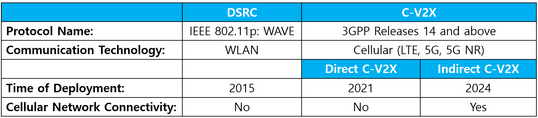
\includegraphics[width=0.6\linewidth]{image/DSRC} \caption{DSRC und C-V2X (Autocrypt, 2021)}\label{fig:unnamed-chunk-48}
\end{figure}

Der Begriff ``\emph{Cellular}'' in C-V2X kann für Verwirrung sorgen. ``\emph{Zellular}'' bezieht sich in diesem Zusammenhang nicht auf die Nutzung von Mobilfunknetzen, sondern auf die Nutzung der zugrunde liegenden Elektronik in Mobilfunkgeräten, die für die direkte Kommunikation von einem Funkgerät zum anderen angepasst sind. Nach (Gettman, 2020) sind die wichtigsten Gemeinsamkeiten und Unterschiede zwischen DSRC- und C-V2X-Technologie die folgenden:

\textbf{Ähnlichkeiten}

\begin{itemize}
\tightlist
\item
  Sowohl DSRC als auch C-V2X nutzen das 5,9-Ghz-Band für die direkte Kommunikation von einem Funkgerät zum anderen.
\item
  Beide Technologien verwenden die gleichen Nachrichtensätze (SAE J2735 und J2945) und Anwendungsfälle.
\item
  Beide Technologien verwenden digitale Signaturen, um die Sicherheit und das Vertrauen in die Nachrichtenanbieter zu gewährleisten.
\item
  In beiden Fällen gibt es keine Verbindung zwischen den Funkgeräten. Jedes Funkgerät überträgt den Standort, die Geschwindigkeit, die Beschleunigung und andere Statuselemente des Fahrzeugs, während es andere Funkgeräte abhört.
\end{itemize}

\textbf{Unterschiede}

\begin{itemize}
\tightlist
\item
  DSRC verwendet einen Funkstandard namens WAVE, während C-V2X Long-Term Evolution (LTE) verwendet - die Chip-Technologie, die fast alle Mobiltelefone nutzen. Ein DSRC-Funkgerät kann nicht mit einem C-V2X-Funkgerät sprechen und umgekehrt.
\item
  Die Reichweite von DSRC beträgt in der Regel 300 m, und viele Installationen haben gezeigt, dass eine viel höhere Reichweite möglich ist. Erste Tests von C-V2X zeigen, dass die Reichweite 20-30 \% größer ist als bei DSRC und dass die Leistung bei Hindernissen deutlich verbessert werden kann. Obwohl C-V2X anfänglich eine bessere Leistung zu haben scheint, ist die Reichweite und Zuverlässigkeit von DSRC für die wichtigsten Sicherheitsanwendungen mehr als ausreichend.
\end{itemize}

Ebenfalls relevant für die drahtlose Kommunikation im Verkehrssektor ist das VANET, ein Ad-hoc-Netz für Fahrzeuge. Es ist eine Unterklasse der mobilen Ad-hoc-Netze (MANETs), wobei es von fahrenden Fahrzeugen gebildet wird. VANET wird zunehmend bei der Bewältigung von Staus im Berufsverkehr eingesetzt. Die größte Herausforderung in VANET ist die Zusammenarbeit zwischen den Knoten. Denn selbst die beste Lenkungskonvention wäre nicht von Vorteil, wenn die Knotenpunkte nicht an der Übermittlung der Informationen teilnehmen (Rath et al., 2019).

\hypertarget{wichtige-interessensgruppen-53}{%
\subsection*{Wichtige Interessensgruppen}\label{wichtige-interessensgruppen-53}}
\addcontentsline{toc}{subsection}{Wichtige Interessensgruppen}

\begin{itemize}
\tightlist
\item
  \textbf{Betroffene}: Fahrer:innen von Personenkraftwagen, Fahrer:innen von Nutzfahrzeugen, Versicherungen
\item
  \textbf{Verantwortliche}: Nationale Regierungen, Technologieunternehmen, Automobilhersteller, Infrastrukturhersteller
\end{itemize}

\hypertarget{aktueller-stand-der-wissenschaft-und-forschung-53}{%
\subsection*{Aktueller Stand der Wissenschaft und Forschung}\label{aktueller-stand-der-wissenschaft-und-forschung-53}}
\addcontentsline{toc}{subsection}{Aktueller Stand der Wissenschaft und Forschung}

Lange vor der Entwicklung von 5G wurde die V2X-Kommunikation untersucht. Viele Analyst:innen und Branchenvertreter:innen gehen davon aus, dass 5G aufgrund der neuen Geschwindigkeiten und anderer technischer Fortschritte in 5G die zukünftige Technologie für die V2X-Kommunikation sein wird. Folglich muss die Sicherheit von 5G und die Frage, wie sie in das aktuelle IVS-Modell integriert werden kann, eingehend untersucht werden (Annu et al., 2021).

Einige Forschungsarbeiten befassen sich mit verschiedenen Materialien und ihren Eigenschaften für die drahtlose Kommunikation (Nitika et al., 2021). Es wird auch bereits an den Spezifikationen für 6G-Antennen für die nächste Generation geforscht. Das Terahertz (THz)-Frequenzband (0,1-10 THz) wird im drahtlosen 6G-Kommunikationssystem verwendet werden, um die Nachfrage der Nutzer:innen nach höheren Datenraten und Ultra-Hochgeschwindigkeits-Kommunikation für viele zukünftige Anwendungen zu unterstützen (Hajiyat et al., 2021). Darüber hinaus testen Zhao et al.~(2019) ein DSRC-basiertes Kollisionswarnsystem, da die Genauigkeit von GPS leicht von der Fahrumgebung betroffen ist, insbesondere wenn es abgeschirmt ist. Die Multi-Sensor-Fusions-Positionierungstechnologie ist eine vielversprechende Methode, um die Genauigkeit der Sicherheitsabstandsberechnung zu verbessern und eine spurgenaue Positionierung zu erreichen.

Mannoni et al.~(2019) verglichen TS-G5 und C-V2X für die V2X-Kommunikationssysteme. Es zeigte sich, dass C-V2X bei gleicher Datenrate eine bessere Flexibilität und Leistung als ITS-G5 aufweist. Basierend auf der Leistung der physikalischen Schicht wurde das Verhalten der beiden Standards in einem Netzwerk ohne Mobilfunkabdeckung und mit mehreren Fahrzeugen bewertet. Die Simulationen zeigten, dass C-V2X bei geringer Nutzerdichte besser abschneidet als ITS-G5. Allerdings verschlechtert sich die Leistung von C-V2X stärker als die von ITS-G5, wenn der Grad der Überlastung zunimmt. Der Vergleich der Ressourcenzugriffszeit (Latenzzeit) zeigt einen Vorteil für ITS-G5, aber die Gesamtlatenz ist nicht eindeutig besser, da sie stark von der Nutzerdichte und der Abdeckung abhängt..

Die Ergebnisse von Sattiraju et al.~(2020) zeigen auch, dass C-V2X die IEEE 802.11p DSRC (ITS-G5) Technologie für fast alle betrachteten Kanalmodelle übertrifft, mit einem Gewinn von 0-5 dB. Außerdem zeigen die Ergebnisse, dass C-V2X bei höheren Fahrzeuggeschwindigkeiten besser abschneidet. Diese bessere Leistung von C-V2X kann auf die Verwendung des Turbo-Encoders und den besseren Kanalschätzungsmechanismus zurückgeführt werden, der eine höhere Anzahl von DMRS-Symbolen verwendet.

Salvo et al.~(2017) haben in ihrer Forschung über heterogene zellulare und DSRC-Netzwerke für die Datenerfassung von Floating Car in städtischen Gebieten gezeigt, dass es sinnvoll ist, sich auf direkte V2V-Kommunikationsverbindungen (ITS-5G) zu verlassen, bevor Daten über LTE-Kanäle (C-V2X) gesendet werden. Die vorgeschlagene Lösung passt sich vollständig an die verfügbare Durchdringungsrate der VANET-Ausrüstung an; sie fällt automatisch auf eine reine LTE-FCD-Erfassung zurück, wenn die VANET-Ausrüstung nicht verfügbar oder zu spärlich ist. Der erreichbare Durchsatz bei der FCD-Erfassung ist ein Schlüsselthema angesichts der enormen Menge an Sensordaten, die potenziell von fahrenden Fahrzeugen erfasst werden können, z. B. können bis zu 100 Mbit/s über den CAN-Bus eines Fahrzeugs übertragen werden (Kang et al., 2016). Diese extremen Echtzeit- und hochauflösenden Big Data erfordern neue Ideen für die verteilte Verarbeitung und Vernetzung, um den Weg für intelligente Anwendungen zu ebnen - ein Trend, der bisher wenig erforscht wurde (Salvo et al., 2017).

\hypertarget{aktueller-stand-der-praktischen-umsetzung-53}{%
\subsection*{Aktueller Stand der praktischen Umsetzung}\label{aktueller-stand-der-praktischen-umsetzung-53}}
\addcontentsline{toc}{subsection}{Aktueller Stand der praktischen Umsetzung}

In Europa ist DSRC die derzeit am häufigsten verwendete Technologie. So brachte VW 2019 seinen Golf 8 mit DSRC-basiertem V2X auf den Markt. Damit wurde Europas beliebtestes Auto zum ersten Massenmarktfahrzeug mit V2X. In anderen Teilen der Welt ging DSRC-basiertes V2X nach einigen groß angelegten Feldversuchen 2015 in Japan und 2017 in den USA in ausgewählten Fahrzeugmodellen in Serie. Während DSRC-basiertes V2X in Europa und Japan eingesetzt wird, gewinnt C-V2X in anderen Regionen an Dynamik. China zum Beispiel treibt die Einführung von C-V2X voran. Anfang 2020 wurde der Chipsatz von Autotalk für ein C-V2X-Massenproduktionsprogramm in China ausgewählt (Autotalks Ltd., n.d.).

DSRC und C-V2X arbeiten mit unterschiedlichen Kommunikationstechnologien, und die Zugangsebene ist nicht interoperabel. Dies stellt Automobilhersteller und Infrastrukturentwickler vor die schwierige Entscheidung, ob sie die eine oder die andere Technologie bevorzugen sollen. Viele Chip-Hersteller arbeiten jedoch an der Produktion von Dual-Mode-Chipsätzen, die mit beiden Standards kompatibel sind, was den Automobilherstellern den Wechsel erleichtert. Was die Infrastrukturentwickler betrifft, so arbeiten viele von ihnen mit bestehenden DSRC-Infrastrukturen, um durch die Kombination mit indirektem C-V2X die Konnektivität mit Mobilfunknetzen zu erhöhen. Unabhängig von den verwendeten Kommunikationstechnologien ist die Cybersicherheit ein wesentlicher Bestandteil von V2X. AutoCrypt V2X ist eine Sicherheitslösung, die sich in V2X-Chipsätze einbettet und das V2X-System sowohl mit Authentifizierungs- als auch Datenverschlüsselungstechnologien schützt (Autocrypt, 2021).

Laut Erhart (2019) wird der Mobilfunk (3G/4G, zukünftig 5G) im Fernverkehr eingesetzt werden. Die C-ROADS-Initiative, in der 18 EU-Mitgliedsstaaten zum Thema C-ITS zusammenarbeiten, strebt nicht nur eine europaweite Harmonisierung und Weiterentwicklung von C-ITS an, sondern auch die Definition der notwendigen Schnittstellen und Datenformate für diese Langstreckenlösung im Mobilfunkbereich. Die ASFINAG ist in diesen Bereichen ein führendes Mitglied der C-ROADS-Initiative und wird beide Kommunikationsarten bei der Umsetzung berücksichtigen.

Die nächste Generation der Kommunikationstechnologie könnte von Unternehmen wie Starlink oder Kuiper initiiert werden, wenn es ihnen gelingt, LEO-Konstellationen aufzubauen (Techbook, 2020). Starlink ist ein Teilunternehmen von Spacex und versucht, ein zusammenhängendes Internet-Netzwerk mit Tausenden von Satelliten aufzubauen, um Hochgeschwindigkeits-Internet auf der ganzen Welt zu liefern (Sheetz, 2021). Starlink-Satelliten sind mehr als 60 Mal näher an der Erde als herkömmliche Satelliten, was zu geringeren Latenzzeiten führt. Starlink eignet sich ideal für Gebiete auf der Welt, in denen die Konnektivität normalerweise eine Herausforderung darstellt (Starlink, n.d.). Allerdings stellen dicht besiedelte städtische Gebiete ein Problem dar (Holland, 2021). Derzeit befinden sich 1100 SpaceX-Satelliten im All, um den globalen Internetdienst aufzubauen. In den kommenden Jahren sollen mehrere tausend weitere Satelliten hinzukommen. Wie ``Golem'' berichtet, sollen es in der vollen Ausbaustufe 12000 Satelliten sein (finanzen.net, 2021). Starlink hat bereits mehr als 500.000 Bestellungen für seinen Satelliten-Internetdienst erhalten. Während Konkurrenten wie OneWeb oder Amazons Project Kuiper hinterherhinken, schafft SpaceX mit Starlink immer mehr Fakten (Holland, 2021). Satelliteninternet ist jedoch für Flugzeuge, Schiffe, große Lastwagen und Wohnmobile gedacht. Für PKWs sind sie noch nicht geeignet, da die Endgeräte dafür einfach viel zu groß sind (Musk, 2021).

Außerdem warnen Forscher:innen vor einigen Folgen für die Astronomie, die dieses Satellitensystem mit sich bringt. Zu den Nachteilen gehört eine kürzere effektive Betriebszeit der Teleskope (aufgrund von Satelliten, die bei Beobachtungen im Weltraum dazwischen sein können), ein höheres Potenzial für Kollisionen mit Forschungsinfrastrukturen, die Erzeugung von Trümmerteilen in der Umlaufbahn und ein erhöhter Bedarf an kostspieligen Ausweichmanövern von Raumschiffen während Weltraummissionen (Traxler \& Rennert, 2020).

\hypertarget{relevante-initiativen-in-uxf6sterreich-53}{%
\subsection*{Relevante Initiativen in Österreich}\label{relevante-initiativen-in-uxf6sterreich-53}}
\addcontentsline{toc}{subsection}{Relevante Initiativen in Österreich}

DSRC-Module werden in Österreich bereits für die LKW-Mautabrechnung eingesetzt. Rund 152.000 Fahrzeuge haben im Jahr 2018 in Österreich über die Toll Collect OBU rund 190 Millionen Euro an Mauteinnahmen generiert. Das DSRC-Modul arbeitet auf Mikrowellenbasis und löst beim Passieren einer Mautstation auf österreichischen Autobahnen und Schnellstraßen eine Mauttransaktion aus, die dann von der Mautstation zur Abrechnung an das Rechenzentrum der ASFINAG übermittelt wird. Die fest im LKW installierte Toll Collect On-Board-Unit zeichnet sich durch hohe Verfügbarkeit und Stabilität aus. In Deutschland erfolgt die Mauterhebung mit der OBU weiterhin über Satellit.

\begin{itemize}
\tightlist
\item
  \href{https://www.toll-collect.de/de/toll_collect/unternehmen/presse/pressemitteilungen/detailseite_press_6241.html}{Toll-collect.de}
\end{itemize}

Eine weitere aktuelle Anwendung von DSRC ist die Fernabfrage von Fahrtenschreiberdaten durch Kontrollbehörden. Seit dem 15. Juni 2019 müssen neue LKW und Busse über 3,5t hzGG mit einem ``Smart Tacho'' ausgestattet sein, der dies ermöglicht (WKÖ, 2019). Derzeit gibt es zwei C-ITS-Testumgebungen: eine rund um Wien und eine bei Graz. Geplant ist eine Ausweitung ab dem Jahr 2020. Zunächst sollen der Korridor Salzburg - Wien, die A2 um Graz und ausgewählte Grenzgebiete abgedeckt werden.

Auf europäischer Ebene hat sich eine Gemeinschaft von Straßenbetreibern, Fahrzeug- und Landmaschinenherstellern, Städten sowie Industrie- und Telekommunikationsunternehmen zu einer Interessengruppe namens ``C-ITS Deployment Group'' zusammengeschlossen. Die Mitglieder dieser Gruppe setzen sich für einen koordinierten C-ITS Einsatz in Europa ein, d.h. C-ITS Dienste sollen in ganz Europa gleich aussehen und von allen Fahrzeugen verstanden werden (Erhart, 2019).

\begin{itemize}
\tightlist
\item
  \href{https://blog.asfinag.at/technik-innovation/c-its-vernetzte-autos-intelligenter-verkehr/}{Asfinag.at}
\end{itemize}

\hypertarget{auswirkungen-in-bezug-auf-die-ziele-fuxfcr-nachhaltige-entwicklung-sdgs-53}{%
\subsection*{Auswirkungen in Bezug auf die Ziele für nachhaltige Entwicklung (SDGs)}\label{auswirkungen-in-bezug-auf-die-ziele-fuxfcr-nachhaltige-entwicklung-sdgs-53}}
\addcontentsline{toc}{subsection}{Auswirkungen in Bezug auf die Ziele für nachhaltige Entwicklung (SDGs)}

\begin{longtable}[]{@{}ccccc@{}}
\toprule
\begin{minipage}[b]{0.17\columnwidth}\centering
Ebene der Auswirkungen\strut
\end{minipage} & \begin{minipage}[b]{0.16\columnwidth}\centering
Indikator\strut
\end{minipage} & \begin{minipage}[b]{0.17\columnwidth}\centering
Richtung der Auswirkungen\strut
\end{minipage} & \begin{minipage}[b]{0.17\columnwidth}\centering
Beschreibung des Ziels \& SDG\strut
\end{minipage} & \begin{minipage}[b]{0.17\columnwidth}\centering
Quelle\strut
\end{minipage}\tabularnewline
\midrule
\endhead
\begin{minipage}[t]{0.17\columnwidth}\centering
Systemisch\strut
\end{minipage} & \begin{minipage}[t]{0.16\columnwidth}\centering
Kontinuierliche Entwicklung der Kommunikationstechnologien\strut
\end{minipage} & \begin{minipage}[t]{0.17\columnwidth}\centering
\textbf{+}\strut
\end{minipage} & \begin{minipage}[t]{0.17\columnwidth}\centering
Innovation und Infrastruktur (\emph{9})\strut
\end{minipage} & \begin{minipage}[t]{0.17\columnwidth}\centering
Techbook, 2020; Autotalks Ltd., n.d.; Salvo et al., 2017\strut
\end{minipage}\tabularnewline
\begin{minipage}[t]{0.17\columnwidth}\centering
Systemisch\strut
\end{minipage} & \begin{minipage}[t]{0.16\columnwidth}\centering
Neue Initiativen und Interessengruppen werden gegruendet\strut
\end{minipage} & \begin{minipage}[t]{0.17\columnwidth}\centering
\textbf{+}\strut
\end{minipage} & \begin{minipage}[t]{0.17\columnwidth}\centering
Partnerschaften und Kooperationen (\emph{17})\strut
\end{minipage} & \begin{minipage}[t]{0.17\columnwidth}\centering
Erhart, 2019\strut
\end{minipage}\tabularnewline
\bottomrule
\end{longtable}

\hypertarget{technologie--und-gesellschaftlicher-bereitschaftsgrad-49}{%
\subsection*{Technologie- und gesellschaftlicher Bereitschaftsgrad}\label{technologie--und-gesellschaftlicher-bereitschaftsgrad-49}}
\addcontentsline{toc}{subsection}{Technologie- und gesellschaftlicher Bereitschaftsgrad}

\begin{longtable}[]{@{}cc@{}}
\toprule
Stand der Technologiebereitschaft & Gesellschaftlicher Bereitschaftsgrad\tabularnewline
\midrule
\endhead
5-8 & 6-8\tabularnewline
\bottomrule
\end{longtable}

\hypertarget{offene-fragen-51}{%
\subsection*{Offene Fragen}\label{offene-fragen-51}}
\addcontentsline{toc}{subsection}{Offene Fragen}

\begin{enumerate}
\def\labelenumi{\arabic{enumi}.}
\tightlist
\item
  Welche alternativen Lösungen gibt es, um DSRC und C-V2X so zu verbinden, dass sie miteinander kompatibel sind?
\end{enumerate}

\hypertarget{weitere-links-44}{%
\subsection*{Weitere links}\label{weitere-links-44}}
\addcontentsline{toc}{subsection}{Weitere links}

\begin{itemize}
\tightlist
\item
  \href{https://c-its-korridor.de/?menuId=1\&sp=en}{C-its-korridor.de}
\item
  \href{https://www.asfinag.at/ueber-uns/newsroom/pressemeldungen/2020/wlan-ausbau-cooperative-intelligent-transport-systems/}{Asfinag.at}
\item
  \href{https://www.autocrypt.io/blog-post/dsrc-vs-c-v2x-detailed-comparison}{Autocrypt.io}
\item
  \href{https://www.kimley-horn.com/news-insights/dsrc-cv2x-comparison-future-connected-vehicles/}{Kimley-horn.com}
\end{itemize}

\hypertarget{referenzen-53}{%
\subsection*{Referenzen}\label{referenzen-53}}
\addcontentsline{toc}{subsection}{Referenzen}

\begin{itemize}
\tightlist
\item
  Annu, Kaushik, D., \& Gupta, A. (2021). Ultra-secure transmissions for 5G-V2X communications. Materials Today: Proceedings. \url{https://doi.org/10.1016/j.matpr.2020.12.130}
\item
  Autocrypt. (2021). AUTOCRYPT - DSRC vs.~C-V2X: A Detailed Comparison of the 2 Types of V2X Technologies. \url{https://www.autocrypt.io/blog-post/dsrc-vs-c-v2x-detailed-comparison}
\item
  Autotalks Ltd.~(n.d.). C-V2X vs DSRC \textbar{} Get Your Facts Straight on Cellular V2X, LTE-V and LTE-V2X Autotalks. Available at: \url{https://www.auto-talks.com/technology/dsrc-vs-c-v2x-2/} {[}Accessed: 4 May 2021{]}
\item
  Erhart, J. (2019, November 28). Vernetzte Autos, intelligenter Verkehr: Was C-ITS ist, was es kann und wem es nutzt.Available at: \url{https://blog.asfinag.at/technik-innovation/c-its-vernetzte-autos-intelligenter-verkehr/} {[}Accessed: 4 May 2021{]}
\item
  Fillenberg, S. (2017, December 18). Cellular V2X: Continental Successfully Conducts Field Trials in China. Continental Press Release. \url{https://www.continental.com/en/press/press-releases/2017-12-18-cellular-v2x-116994}
\item
  finanzen.net. (2021, May 5). Internet aus dem All: Internetsparte von SpaceX: Starlink bald in Wohnmobilen, Schiffen und Flugzeugen? \textbar{} Nachricht \textbar{} finanzen.net. \url{https://www.finanzen.net/nachricht/geld-karriere-lifestyle/internet-aus-dem-all-internetsparte-von-spacex-starlink-bald-in-wohnmobilen-schiffen-und-flugzeugen-9905140}
\item
  Gettman, D. (2020, June 3). DSRC and C-V2X: The Future of Connected Vehicles \textbar{} Kimley-Horn. \url{https://www.kimley-horn.com/news-insights/dsrc-cv2x-comparison-future-connected-vehicles/}
\item
  Hajiyat, Z. R. M., Ismail, A., Sali, A., \& Hamidon, M. N. (2021). Antenna in 6G wireless communication system: Specifications, challenges, and research directions. Optik, 231(February), 166415. \url{https://doi.org/10.1016/j.ijleo.2021.166415}
\item
  Holland, M. (2021, May 5). Starlink: Schon 500.000 Vorbestellungen für Satelliten-Internet von SpaceX \textbar{} heise online. \url{https://www.heise.de/news/Starlink-Schon-500-000-Vorbestellungen-fuer-Satelliten-Internet-von-SpaceX-6036732.html}
\item
  IEEE. (2014). IEEE Guide for Wireless Access in Vehicular Environments (WAVE) - Architecture. IEEE Std 1609.0-2013, 1--78. \url{https://doi.org/10.1109/IEEESTD.2014.6755433}
\item
  Kang, S., Han, S., Cho, S., Jang, D., Choi, H., \& Choi, J.-W. (2016). High speed CAN transmission scheme supporting data rate of over 100 Mb/s. IEEE Communications Magazine, 54(6), 128--135. \url{https://doi.org/10.1109/MCOM.2016.7498099}
\item
  Mannoni, V., Berg, V., Sesia, S., \& Perraud, E. (2019). A comparison of the V2X communication systems: ITS-G5 and C-V2X. IEEE Vehicular Technology Conference, 2019-April. \url{https://doi.org/10.1109/VTCSpring.2019.8746562}
\item
  Musk, E. (2021, March 7). Elon Musk auf Twitter. \url{https://twitter.com/elonmusk/status/1369051431903268865?ref_src=twsrc\%5Etfw\%7Ctwcamp\%5Etweetembed\%7Ctwterm\%5E1369051431903268865\%7Ctwgr\%5E\%7Ctwcon\%5Es1}
\item
  Nitika, Rana, A., Kumar, V., \& Awasthi, A. M. (2021). Effect of dopant concentration and annealing temperature on electric and magnetic properties of lanthanum substituted CoFe2O4 nanoparticles for potential use in 5G wireless communication systems. Ceramics International. \url{https://doi.org/10.1016/j.ceramint.2021.04.077}
\item
  Rath, M., Pati, B., \& Pattanayak, B. K. (2019). An Overview on Social Networking: Design, Issues, Emerging Trends, and Security. In Social Network Analytics (pp.~21--47). Elsevier. \url{https://doi.org/10.1016/b978-0-12-815458-8.00002-5}
\item
  Salvo, P., Turcanu, I., Cuomo, F., Baiocchi, A., \& Rubin, I. (2017). Heterogeneous cellular and DSRC networking for Floating Car Data collection in urban areas. Vehicular Communications, 8, 21--34. \url{https://doi.org/10.1016/j.vehcom.2016.11.004}
\item
  Sattiraju, R., Wang, D., Weinand, A., \& Schotten, H. D. (2020). Link level performance comparison of C-V2X and ITS-G5 for vehicular channel models. ArXiv, March.
\item
  Sheetz, M. (2021, May 4). SpaceX: Over 500,000 orders for Starlink satellite internet service. Available at: \url{https://www.cnbc.com/2021/05/04/spacex-over-500000-orders-for-starlink-satellite-internet-service.html} {[}Accessed: 4 May 2021{]}
\item
  Starlink. (n.d.). Starlink. Available at: \url{https://www.starlink.com/} {[}Accessed: 6 May 2021{]}
\item
  Techbook. (2020, November 16). LTE, 4G und 5G: Die Unterschiede zwischen den Mobilfunkstandards.Available at: \url{https://www.techbook.de/mobile/lte-4g-unterschied-mobil-smartphone} {[}Accessed: 4 May 2021{]}
\item
  Traxler, T., \& Rennert, D. (2020, February 17). Starlink: Elon Musks Satellitenflotte in der Kritik - Raum - derStandard.at › Wissenschaft.Available at: \url{https://www.derstandard.at/story/2000114681438/starlink-elon-musks-satellitenflotte-in-der-kritik} {[}Accessed: 4 May 2021{]}
\item
  WKÖ. (2019). Ausrüstungspflicht von neuen lkw und omnibussen mit einem „smart tacho`` ab 15. Juni 2019. Available at: \url{https://www.google.com/url?sa=t\&rct=j\&q=\&esrc=s\&source=web\&cd=\&ved=2ahUKEwiyka_Xs7XwAhXytYsKHTq_AJ0QFjADegQIBBAD\&url=https\%3A\%2F\%2Fwww.wko.at\%2Fbranchen\%2Ftransport-verkehr\%2Fausruestungspflicht-smart-tacho.pdf\&usg=AOvVaw12-xLPvw33KN9gvYKy51tn} {[}Accessed: 4 May 2021{]}
\item
  Zhao, X., Jing, S., Hui, F., Liu, R., \& Khattak, A. J. (2019). DSRC-based rear-end collision warning system -- An error-component safety distance model and field test. Transportation Research Part C: Emerging Technologies, 107, 92--104. \url{https://doi.org/10.1016/j.trc.2019.08.002}
\end{itemize}

\hypertarget{bd_life}{%
\section{Big data Lebenszyklus}\label{bd_life}}

\hypertarget{definition-54}{%
\subsection*{Definition}\label{definition-54}}
\addcontentsline{toc}{subsection}{Definition}

``\emph{Big Data bezieht sich auf große Datensätze, die heterogene Formate umfassen: strukturierte, unstrukturierte und semistrukturierte Daten. Big Data ist von komplexer Natur und erfordert leistungsstarke Technologien und fortschrittliche Algorithmen. Daher können die traditionellen statischen Business Intelligence-Tools bei Big Data-Anwendungen nicht mehr effizient sein}'' (Oussous et al., 2018). Big Data ist typischerweise durch die 3Vs (Volume, Velocity und Variety) gekennzeichnet, wie im Thema \protect\hyperlink{bd_tool_maping}{Big Data Tools} beschrieben. Im Verkehrskontext sind die wichtigsten Quellen von Big Data:

\begin{itemize}
\tightlist
\item
  Fahrerassistenzsysteme und instrumentierte Fahrzeuge, die die Fahrzeugumgebung und das Fahrverhalten ständig überwachen
  Yuan et al.~(2015) behauptet, dass vernetzte Fahrzeuge sogar 30 GB an Daten pro Tag produzieren könnten.
\item
  Informationssysteme für Reisende
\item
  Straßenbetrieb und -management wie \protect\hyperlink{variable_speed}{variable Geschwindigkeitsbegrenzungen und dynamische Beschilderungssysteme}
\item
  Verkehrsdaten
  Zum Beispiel {[}Echtzeit-Verkehrsinformationen und -überwachung{]},(\#traffic\_info\_monitoring) die strukturierte und unstrukturierte Daten wie JPG, JSON, GPS, PDF, Bilder, Videos und Beiträge in sozialen Medien erzeugen können (Kemp et al., 2015)
\item
  Notfall- und Störfallmanagement
\end{itemize}

Die in Neilson et al.~(2019) zusammengefasste Literatur zeigt die folgende Verwendung von Big Data im Verkehrskontext:

\begin{longtable}[]{@{}cccc@{}}
\toprule
\begin{minipage}[b]{0.22\columnwidth}\centering
Verwendete Big-Data-Systeme\strut
\end{minipage} & \begin{minipage}[b]{0.22\columnwidth}\centering
Zwecke der Big-Data-Analyse\strut
\end{minipage} & \begin{minipage}[b]{0.22\columnwidth}\centering
Arten der erfassten Daten\strut
\end{minipage} & \begin{minipage}[b]{0.22\columnwidth}\centering
Aktuelle Chancen und Herausforderungen\strut
\end{minipage}\tabularnewline
\midrule
\endhead
\begin{minipage}[t]{0.22\columnwidth}\centering
ITS, Hadoop, MapReduce, Batch- und Stream-Datenverarbeitung, NoSQL\strut
\end{minipage} & \begin{minipage}[t]{0.22\columnwidth}\centering
Stadtplanung, Analyse von Kollisionen und Beinaheunfaellen, Verkehrsueberlastung, Sicherheit, Optimierung\strut
\end{minipage} & \begin{minipage}[t]{0.22\columnwidth}\centering
Geschwindigkeit, Standort, Video, Bild, Verkehrsintensitaet, soziale Medien, Crowdsourcing, maschinelles Lernen, historische, Echtzeit-, praediktive, visuelle, Video-/Bildanalyse\strut
\end{minipage} & \begin{minipage}[t]{0.22\columnwidth}\centering
Datenerhebung, -qualitaet, -speicherung, -verarbeitung, Datenschutz, Sicherheit, vernetzte und automatisierte Fahrzeuge\strut
\end{minipage}\tabularnewline
\bottomrule
\end{longtable}

Ein weiterer wichtiger Teil von Big Data ist der Lebenszyklus, auch Informationslebenszyklus genannt, der als der Zeitraum definiert ist, in dem die Daten im System vorhanden sind. Dieser Lebenszyklus umfasst alle Phasen, die die Daten von der ersten Erfassung an durchlaufen (Talend.com, 2021). In der aktuellen Literatur werden verschiedene Modelle vorgeschlagen, die von der Art der Daten und dem jeweiligen Bereich abhängen. Nichtsdestotrotz weisen sie einige Ähnlichkeiten auf, und die meisten Phasen werden von den meisten Datenzyklusmodellen geteilt. Nach Arras \& Souissi (2018) sind die wichtigsten Phasen des Big Data Lifecycle folgende:

\begin{itemize}
\tightlist
\item
  \emph{Planung}: Eine detaillierte Beschreibung, wie Daten während ihres Lebenszyklus genutzt, verwaltet und zugänglich gemacht werden sollen
\item
  \emph{Management}: Umfasst alle operativen Phasen, in denen die Daten direkt bearbeitet werden
\item
  \emph{Sammlung}: Sie besteht aus dem Empfang der Rohdaten verschiedener Typen und der Durchführung der für ihre Organisation erforderlichen Umwandlungen und Änderungen. Die Bereinigung der in Echtzeit empfangenen Daten spart Rechenzeit und Speicherplatz. Die Datenqualität muss auf dieser Ebene durchgeführt werden, da sie eine Optimierung des gesamten Datenverarbeitungskreislaufs ermöglicht.
\item
  \emph{Integration}: In dieser Phase geht es darum, ein kohärentes Muster von Daten aus mehreren unabhängigen, verteilten und heterogenen Informationsquellen bereitzustellen, um den Benutzer:innen den Zugriff und die Abfrage dieser Daten zu erleichtern, als ob sie auf eine einzige Datenquelle zugreifen würden
\item
  \emph{Filtern}: Besteht in der Einschränkung des großen Datenstroms, um irrelevante Daten oder Fehler zu entfernen
\item
  \emph{Anreicherung}: Bei der Datenanreicherung werden strukturelle oder hierarchische Änderungen an den empfangenen Daten vorgenommen. Sie ermöglicht das Hinzufügen von Informationen zu den gesammelten Daten, um deren Qualität zu verbessern.
\item
  \emph{Analyse}: In dieser Phase werden die Daten ausgewertet und analysiert, um Schlussfolgerungen und Interpretationen für die Entscheidungsfindung zu ziehen
\item
  \emph{Zugang}: In dieser Phase geht es um die Kommunikation/Interaktion mit den Datenkonsument:innen
\item
  \emph{Visualisierung}: Sie besteht darin, die Ergebnisse der Analyse in einer übersichtlichen Form darzustellen, so dass die Entscheidungsträger:innen diese Ergebnisse leicht verstehen und fundierte Entscheidungen treffen können
\item
  \emph{Speicherung}: Betrifft alle anderen Phasen des Zyklus und ermöglicht die Speicherung der Daten während ihres gesamten Lebenszyklus, um eine kontinuierliche Rückverfolgbarkeit der Daten in jeder Phase des Zyklus zu gewährleisten
\item
  \emph{Vernichtung}: In dieser Phase werden die Daten entsorgt, wenn sie erfolgreich genutzt wurden und somit nutzlos und ohne Mehrwert sind.
\item
  \emph{Archivierung}: Besteht aus einer Implementierung von Datensicherheit und Vertraulichkeit
\end{itemize}

Darüber hinaus haben Djahel et al.~(2014) einen Big-Data-Lebenszyklus in Bezug auf Verkehrsmanagementsysteme (TMS) vorgeschlagen, der in Abbildung 12.2 dargestellt ist.

\begin{figure}
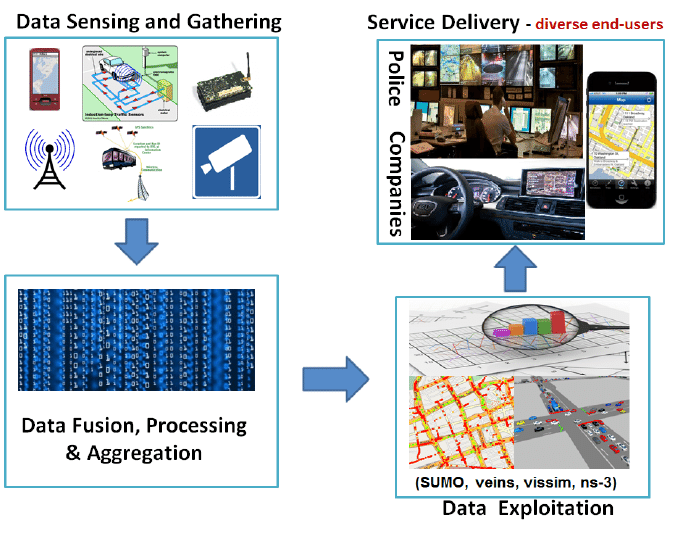
\includegraphics[width=0.75\linewidth]{image/BDLC} \caption{Lebenszyklus von Big Data im intelligenten Verkehrswesen (Djahel et al., 2014)}\label{fig:unnamed-chunk-50}
\end{figure}

In der ersten Phase der \emph{Datenerfassung und -sammlung (Data Sensing and Gathering, DSG)} werden die Verkehrsdaten überwacht und gesammelt, um Informationen über das Verkehrsaufkommen, Zwischenfälle, die Auslastung oder die Geschwindigkeit zu erhalten. Die gesammelten Daten fließen später in die zweite Phase der \emph{Datenfusion, -verarbeitung und -aggregation} ein, in der die relevanten Informationen aus den Rohdaten extrahiert werden. In der dritten Phase, der \emph{Datenauswertung}, werden die verarbeiteten Daten zur Berechnung optimaler Routen, zur Erstellung von Prognosen und zur Erstellung von Verkehrsstatistiken verwendet. In der Phase der \emph{Bereitstellung von Diensten} schließlich teilt das TMS das Wissen mit den Endnutzer:innen wie Fahrer:innen, Behörden oder Fahrgästen über eine Vielzahl von Geräten wie Smartphones oder Bordeinheiten von Fahrzeugen.

\hypertarget{wichtige-interessensgruppen-54}{%
\subsection*{Wichtige Interessensgruppen}\label{wichtige-interessensgruppen-54}}
\addcontentsline{toc}{subsection}{Wichtige Interessensgruppen}

\begin{itemize}
\tightlist
\item
  \textbf{Betroffene}: Fahrgäste, Fahrer:innen, auf ITS spezialisierte Unternehmen
\item
  \textbf{Verantwortliche}: Nationale Regierungen, Technologieunternehmen, auf IVS spezialisierte Unternehmen, Verkehrsunternehmen, Entwickler von Verkehrssoftware
\end{itemize}

\hypertarget{aktueller-stand-der-wissenschaft-und-forschung-54}{%
\subsection*{Aktueller Stand der Wissenschaft und Forschung}\label{aktueller-stand-der-wissenschaft-und-forschung-54}}
\addcontentsline{toc}{subsection}{Aktueller Stand der Wissenschaft und Forschung}

Wie bereits erwähnt, gibt es in der Literatur verschiedene Modelle des Lebenszyklus von Big Data, die über das von Arras \& Souissi (2018) vorgeschlagene Modell des Smart Data Lifecycle (DLC) hinausgehen. Nach Alshboul et al.~(2015) beispielsweise umfasst der Lebenszyklus von Big Data vier Phasen:

\begin{itemize}
\tightlist
\item
  \emph{Datenerfassung}
  Daten aus verschiedenen Quellen kommen in unterschiedlichen Formaten: Strukturiert, halbstrukturiert und unstrukturiert.
\item
  \emph{Speicherung der Daten}
  Die gesammelten Daten werden gespeichert und für die Verwendung in der nächsten Phase vorbereitet. Da die gesammelten Daten sensible Informationen enthalten können, ist es wichtig, bei der Datenspeicherung ausreichende Vorsichtsmaßnahmen zu treffen (z. B. Permutation, Anonymisierung).
\item
  \emph{Datenanalytik}
  Die Daten werden analysiert, um nützliches Wissen zu generieren. In dieser Phase werden Data-Mining-Methoden wie Clustering, Klassifizierung und Assoziationsregel-Mining eingesetzt.
\item
  \emph{Schaffung von Wissen}
  Die Ergebnisse der Analysen werden von den Entscheidungsträger:innen genutzt.
\end{itemize}

Demchenko et al.~(2014) schlagen ein Big Data Lifecycle Management (BDLM) Modell vor, das aus sechs Phasen besteht:

\begin{itemize}
\tightlist
\item
  Datenquelle
\item
  Datenerfassung
\item
  Datenbereinigung (Filterung, Klassifizierung)
\item
  Datenanalytik
\item
  Visualisierung von Daten
\item
  Anwendung der Datenanalyse
\end{itemize}

\hypertarget{aktueller-stand-der-praktischen-umsetzung-54}{%
\subsection*{Aktueller Stand der praktischen Umsetzung}\label{aktueller-stand-der-praktischen-umsetzung-54}}
\addcontentsline{toc}{subsection}{Aktueller Stand der praktischen Umsetzung}

The typical management tools, techniques and software used Die typischen Verwaltungstools, -techniken und -software für die Datenverarbeitung sind Google BigTable, Simple DB, Not Only SQL (NoSQL), Data Stream Management System (DSMS), MemcacheDB und Voldemort. Es werden jedoch ständig neue Anwendungen mit höheren Fähigkeiten entwickelt, um den Anforderungen von Big Data gerecht zu werden (Chen et al., 2014). \href{https://hadoop.apache.org/}{Hadoop} zum Beispiel wurde speziell für die Verwaltung von Big Data in verschiedenen Phasen ihres Lebenszyklus entwickelt. Es handelt sich um ein Open-Source-Software-Framework, das die Verarbeitung großer Datensätze in Computerclustern mithilfe einfacher Programmiermodelle wie Google MapReduce ermöglicht (Khan et al., 2014). Hadoop kann extrem große Datenmengen mit unterschiedlichen Strukturen (oder ohne jegliche Struktur) verarbeiten. Es wird in der Regel auf große Datenmengen angewandt und ermöglicht die Verarbeitung von Daten, die zuvor schwer zu verwalten und zu analysieren waren.

Ein Beispiel aus der Praxis: Big Data in Verbindung mit dem Internet der Dinge (IoT) wird von Data Mill North's National Public Transport Access Nodes (NaPTAN) im Vereinigten Königreich genutzt, um den Fahrgästen Verkehrsinformationen in Echtzeit zu liefern. So nutzen Bahnbetreiber bereits Big Data, um Informationen über die Verfügbarkeit von Sitzplätzen in Echtzeit anzubieten (Rayner, 2017).

\hypertarget{relevante-initiativen-in-uxf6sterreich-54}{%
\subsection*{Relevante Initiativen in Österreich}\label{relevante-initiativen-in-uxf6sterreich-54}}
\addcontentsline{toc}{subsection}{Relevante Initiativen in Österreich}

\begin{itemize}
\tightlist
\item
  \href{https://confare.at/wiener-linien-digitale-zukunft/}{Wiener Linien}
\end{itemize}

\hypertarget{auswirkungen-in-bezug-auf-die-ziele-fuxfcr-nachhaltige-entwicklung-sdgs-54}{%
\subsection*{Auswirkungen in Bezug auf die Ziele für nachhaltige Entwicklung (SDGs)}\label{auswirkungen-in-bezug-auf-die-ziele-fuxfcr-nachhaltige-entwicklung-sdgs-54}}
\addcontentsline{toc}{subsection}{Auswirkungen in Bezug auf die Ziele für nachhaltige Entwicklung (SDGs)}

\begin{longtable}[]{@{}ccccc@{}}
\toprule
\begin{minipage}[b]{0.17\columnwidth}\centering
Ebene der Auswirkungen\strut
\end{minipage} & \begin{minipage}[b]{0.16\columnwidth}\centering
Indikator\strut
\end{minipage} & \begin{minipage}[b]{0.17\columnwidth}\centering
Richtung der Auswirkungen\strut
\end{minipage} & \begin{minipage}[b]{0.17\columnwidth}\centering
Beschreibung des Ziels \& SDG\strut
\end{minipage} & \begin{minipage}[b]{0.17\columnwidth}\centering
Quelle\strut
\end{minipage}\tabularnewline
\midrule
\endhead
\begin{minipage}[t]{0.17\columnwidth}\centering
Systemisch\strut
\end{minipage} & \begin{minipage}[t]{0.16\columnwidth}\centering
Erhoehte Sicherheit fuer Fahrer:innen und Fahrgaeste oeffentlicher Verkehrsmittel\strut
\end{minipage} & \begin{minipage}[t]{0.17\columnwidth}\centering
\textbf{+}\strut
\end{minipage} & \begin{minipage}[t]{0.17\columnwidth}\centering
Gesundheit und Wohlbefinden (\emph{3})\strut
\end{minipage} & \begin{minipage}[t]{0.17\columnwidth}\centering
Rayner, 2017\strut
\end{minipage}\tabularnewline
\begin{minipage}[t]{0.17\columnwidth}\centering
Systemisch\strut
\end{minipage} & \begin{minipage}[t]{0.16\columnwidth}\centering
Erhoehter Energieverbrauch\strut
\end{minipage} & \begin{minipage}[t]{0.17\columnwidth}\centering
\textbf{-}\strut
\end{minipage} & \begin{minipage}[t]{0.17\columnwidth}\centering
Oekologische Nachhaltigkeit (\emph{7,12-13,15})\strut
\end{minipage} & \begin{minipage}[t]{0.17\columnwidth}\centering
Lovell, 2018\strut
\end{minipage}\tabularnewline
\begin{minipage}[t]{0.17\columnwidth}\centering
Systemisch\strut
\end{minipage} & \begin{minipage}[t]{0.16\columnwidth}\centering
Potenzial fuer eine zuverlaessigere und transparentere Partnerschaft entlang der Lieferkette\strut
\end{minipage} & \begin{minipage}[t]{0.17\columnwidth}\centering
\textbf{+}\strut
\end{minipage} & \begin{minipage}[t]{0.17\columnwidth}\centering
Partnerschaften und Kooperationen (\emph{17})\strut
\end{minipage} & \begin{minipage}[t]{0.17\columnwidth}\centering
Robins, 2021\strut
\end{minipage}\tabularnewline
\bottomrule
\end{longtable}

\hypertarget{technologie--und-gesellschaftlicher-bereitschaftsgrad-50}{%
\subsection*{Technologie- und gesellschaftlicher Bereitschaftsgrad}\label{technologie--und-gesellschaftlicher-bereitschaftsgrad-50}}
\addcontentsline{toc}{subsection}{Technologie- und gesellschaftlicher Bereitschaftsgrad}

\begin{longtable}[]{@{}cc@{}}
\toprule
Stand der Technologiebereitschaft & Gesellschaftlicher Bereitschaftsgrad\tabularnewline
\midrule
\endhead
5-9 & 6-9\tabularnewline
\bottomrule
\end{longtable}

\hypertarget{offene-fragen-52}{%
\subsection*{Offene Fragen}\label{offene-fragen-52}}
\addcontentsline{toc}{subsection}{Offene Fragen}

\begin{enumerate}
\def\labelenumi{\arabic{enumi}.}
\tightlist
\item
  Wie lässt sich das Potenzial für Cyberangriffe verringern und wie können die Sicherheitsmethoden verbessert werden?
\item
  Wie kann das Problem, dass Daten in deutschsprachigen Ländern als Bedrohung angesehen werden, gemildert werden?
\end{enumerate}

\hypertarget{referenzen-54}{%
\subsection*{Referenzen}\label{referenzen-54}}
\addcontentsline{toc}{subsection}{Referenzen}

\begin{itemize}
\tightlist
\item
  Alshboul, Y., Nepali, R. K., \& Wang, Y. (2015, August). Big Data LifeCycle: Threats and Security Model. In AMCIS.
\item
  Chen, M., Mao, S., \& Liu, Y. (2014). Big data: A survey. Mobile networks and applications, 19(2), 171-209.
\item
  Demchenko, Y., De Laat, C., \& Membrey, P. (2014, May). Defining architecture components of the Big Data Ecosystem. In 2014 International conference on collaboration technologies and systems (CTS) (pp.~104-112). IEEE.
\item
  Djahel, S., Doolan, R., Muntean, G. M., \& Murphy, J. (2014). A communications-oriented perspective on traffic management systems for smart cities: Challenges and innovative approaches. IEEE Communications Surveys \& Tutorials, 17(1), 125-151.
\item
  El Arass, M., \& Souissi, N. (2018, October). Data lifecycle: From big data to smartdata. In 2018 IEEE 5th international congress on information science and technology (CiSt) (pp.~80-87). IEEE.
\item
  Kemp, G., Vargas-Solar, G., Da Silva, C. F., \& Ghodous, P. (2015, May). Aggregating and managing big realtime data in the cloud-application to intelligent transport for smart cities. In Proceedings of the 1st international conference on vehicle technology and intelligent transport systems (pp.~107-112).
\item
  Khan, N., Yaqoob, I., Hashem, I. A. T., Inayat, Z., Mahmoud Ali, W. K., Alam, M., \ldots{} \& Gani, A. (2014). Big data: survey, technologies, opportunities, and challenges. The scientific world journal, 2014.
\item
  Neilson, A., Daniel, B., \& Tjandra, S. (2019). Systematic review of the literature on big data in the transportation domain: Concepts and applications. Big Data Research, 17, 35-44.
\item
  Oussous, A., Benjelloun, F. Z., Lahcen, A. A., \& Belfkih, S. (2018). Big Data technologies: A survey. Journal of King Saud University-Computer and Information Sciences, 30(4), 431-448.
  Rayner, T. (2017). Deriving Transport Benefits from Big Data and the Internet of Things in Smart Cities. Available at: \url{https://www.womblebonddickinson.com/uk/insights/articles-and-briefings/deriving-transport-benefits-big-data-and-internet-things-smart} {[}Accessed: 12 August 2021{]}
\item
  Robins, C. (2021). WHY BIG DATA IS SO IMPORTANT TO THE TRANSPORTATION INDUSTRY Available at: \url{https://www.robinsconsulting.com/why-big-data-is-so-important/} {[}Accessed: 12 August 2021{]}
\item
  Talend.com (2021). Data Lifecycle Management (Definition and Framework). Available at: \url{https://www.talend.com/resources/data-lifecycle-management/} {[}Accessed: 12 August 2021{]}.
\item
  Yuan, W., Deng, P., Taleb, T., Wan, J., \& Bi, C. (2015). An unlicensed taxi identification model based on big data analysis. IEEE Transactions on Intelligent Transportation Systems, 17(6), 1703-1713.
\end{itemize}

\hypertarget{bd_tool_maping}{%
\section{Big-Data-Tools für die Kartierung und Vorhersage des Reiseverhaltens}\label{bd_tool_maping}}

\hypertarget{synonyme-47}{%
\subsection*{Synonyme}\label{synonyme-47}}
\addcontentsline{toc}{subsection}{Synonyme}

\emph{Anwendungsprogrammierschnittstelle (API - application programming interface)}

\hypertarget{definition-55}{%
\subsection*{Definition}\label{definition-55}}
\addcontentsline{toc}{subsection}{Definition}

\textbf{(Echtzeit-)Verkehrskartierung}
Die Verkehrskartierung erfolgt zum einen mit Verkehrssensoren und zum anderen mit Smartphone-Daten. Staatliche Verkehrsämter haben damit begonnen, solarbetriebene Verkehrssensoren an Hauptverkehrsstraßen im ganzen Land zu installieren, um die aktuelle Verkehrssituation zu erfassen, Planungsstatistiken zu erstellen, die Reaktionszeiten bei Unfällen zu verbessern und den Verkehrsfluss zu erhöhen. Die Daten werden mit verschiedenen Arten von Verkehrssensoren erfasst. In den letzten Jahren haben sich drei oberirdische Typen durchgesetzt: Radar, Aktiv-Infrarot und Laserradar. Die Radarsensorik gibt es bereits seit dem Zweiten Weltkrieg, als sie dem Militär half, feindliche Schiffe in der Luft und auf See zu verfolgen. Die heutige Technologie ermöglicht es jedem dieser Geräte, mehrere Verkehrsspuren gleichzeitig zu überwachen (Machay, n.d.).

Google Maps ist ein wichtiger Akteur auf dem Gebiet der Navigation und Verkehrskartierung. Bis März 2012 gab es keine Verkehrsfunktion - man konzentrierte sich lediglich darauf, die Nutzer:innen von A nach B zu bringen. Es gab zwar eine Funktion, die anzeigte, wie sehr der Verkehr eine:n Fahrer:in aufhalten würde, aber es gab keine Live-Daten. Damals wurden nur historische Daten verwendet, um zu zeigen, wie lange dieselbe Strecke ``bei starkem Verkehr'' dauern würde (NCTA, 2013).

Dann wurde mit den Verkehrsbehörden eine Vereinbarung getroffen, einerseits die von den Sensoren generierten Daten gemeinsam zu nutzen, und andererseits konnten Smartphone-Daten für Echtzeitdaten verwendet werden. Die Daten der Verkehrssensoren der Verkehrsbehörden ermöglichten es Google, seine Verkehrsdienste zu erweitern, während die Verkehrsbehörden einen Teil der Kosten für die Sensoren übernehmen konnten. Durch die Zusammenarbeit mit verschiedenen Verkehrsbehörden erhielt Google aktuelle Informationen über Staus auf Autobahnen und Hauptverkehrsstraßen, war aber kaum in der Lage, den Verkehr auf kleineren Landstraßen und in Wohngebieten zu überwachen. Die aktuellen Verkehrsdaten werden hauptsächlich über GPS-fähige Mobiltelefone gesammelt, auf denen die Anwendung Google Maps läuft. Diese übertragen kontinuierlich den Standort und die Geschwindigkeit von allen Nutzer:innen in Echtzeit an Google. Mithilfe einer als ``Crowdsourcing'' bekannten Technik kombiniert Google die von Tausenden von aktiven Mobiltelefonen gelieferten Informationen, um zu ermitteln, wie schnell der Verkehr an einem bestimmten Ort fließt (Machay, n.d.). Was den Datenschutz betrifft, so behauptet Google, dass die Nutzer:innen in den Einstellungen ihres Telefons entscheiden können, ob sie ihre Reisedaten mit Google teilen wollen oder nicht. Das Unternehmen weist darauf hin, dass es versucht, die Informationen zu schützen (Google selbst weiß nicht einmal, welche Daten von welchem Auto stammen, und es schneidet die ersten und letzten Minuten jeder Fahrt ab, um sie noch unkenntlicher zu machen). Wenn die Nutzer:innen sich dafür entscheiden, tragen sie dazu bei, einen hilfreichen Dienst zu erbringen - die Nutzer:innen erhalten realistischere Schätzungen über die Dauer ihrer Fahrt und können sich besser auf den Verkehr einstellen. Mike Dobson (Präsident von Telemapics) stellt sich ein Zukunftsszenario vor, in dem Google 5 \% der Nutzer:innen Umleitungen vorschlagen könnte, um entweder Verkehrsstaus zu entschärfen oder die Wahrscheinlichkeit von Verspätungen zu verringern. Zhan Guo, Professor für Verkehrspolitik an der New York University, sagt, dass es schwierig sein wird, Ratschläge zur Umleitung des Verkehrs zu geben, da Fahrer:innen, die eine Strecke täglich fahren, am besten wissen, was am längsten dauert. Wenn es nur wenige andere Wege gibt, um von A nach B zu kommen, ist es sinnlos, Alternativen vorzuschlagen, denn jeder wird sich beeilen, eine andere Straße zu verstopfen. Ein Algorithmus, der genau die richtige Menge an Verkehr umleitet, ist seiner Meinung nach wahrscheinlich noch einige Jahre entfernt (NCTA, 2013).

Aufgrund der zunehmenden Verbreitung von Mobiltelefonen mit eingebauten Standort- und Bewegungssensoren in der Bevölkerung können umfangreiche und dynamische Daten gesammelt werden. Mobiltelefondaten ermöglichen eine noch nie dagewesene Abdeckung der Bevölkerung und des geografischen Gebiets (Wang et al., 2018). Die Nachteile dieser Systeme bestehen darin, dass Radarsensoren keine liegengebliebenen Fahrzeuge erkennen können, da sie keine Objekte erkennen können, die sich nicht bewegen. Aktiv-Infrarot- und Laser-Radarsensoren funktionieren bei dichtem Nebel oder Schneetreiben nicht richtig. Und die Genauigkeit des Crowdsourcing kann beeinträchtigt werden, wenn nicht genügend Mobiltelefone Daten für ein bestimmtes Gebiet liefern (Machay, n.d.).

\textbf{Verkehrsprognose}
Um die Verkehrsnachfrage zu prognostizieren, werden Informationen über die Vergangenheit, den Zustand des Verkehrssystems und sein externes System berücksichtigt. Verkehrsprognosemethoden lassen sich je nach mathematischen Methoden und Berechnungsverfahren in verschiedene Typen unterteilen, z. B. qualitativ und quantitativ, linear und nichtlinear, dynamisch und statisch, aggregiert und disaggregiert (Zhao et al., 2018).

Seit den 1950er Jahren dominiert das ``Vier-Stufen-Modell'' die Methoden der Reisebedarfsprognose. Seit den 1970er Jahren haben tätigkeitsbasierte Prognosemethoden mehr Aufmerksamkeit auf sich gezogen.

\textbf{Reiseprognosemethoden}
Trip-basierte Methoden der Reisebedarfsprognose unterteilen die Einheit der Reiseprognose in der Regel in ein ``Aggregat'' (Verkehrsgebiet) und konzentrieren sich auf die Bevölkerung und Flächennutzung des Verkehrsgebiets. Diese Methoden berücksichtigen im Allgemeinen die räumliche Koordination auf Stadtebene, ignorieren aber die tatsächlichen Reisebedürfnisse und Empfindungen der einzelnen Einwohner:innen. Aufgrund der geringen Flexibilität und des geringen Verfeinerungsgrads der Vorhersageergebnisse können diese Methoden daher leicht zu Problemen mit einer ungleichmäßigen Verkehrsverteilung führen (Qin et al., 2013).

Es gibt mehrere reisebasierte Prognosemethoden. Zhao et al.~(2018) führen 5 grundlegende Methoden mit Vorteilen und Einschränkungen auf:

\begin{itemize}
\tightlist
\item
  Graue Systemtheorie (GST)
  In diesem System sind einige Informationen bekannt und einige Informationen unbekannt. Sie ist für kurzfristige Prognosen auf der Grundlage herkömmlicher Umfragedaten fast unmöglich zu verwenden.
\item
  Kalman-Filterung (KF)
  Sie kann den Zustand des dynamischen Systems aus einer Reihe von unvollständigen und verrauschten Messungen schätzen.
\item
  Chaostheorie (CT)
  Sie befasst sich mit der geordneten Struktur und Regelmäßigkeit von scheinbar zufälligen Phänomenen in dynamischen Systemen. Es wird jedoch eine große Menge an Verkehrsüberwachungsdaten als Trainings- oder Entscheidungsmuster benötigt. Aufgrund der Datenerfassung, -eingabe, -übertragung und -speicherung erfordern diese Methoden eine langwierige Vorverarbeitung der Daten und haben nur begrenzte Echtzeitfähigkeiten.
\item
  Künstliches Neuronales Netz (ANN)
  Ein mathematisches Modell, das die Struktur und Funktion von biologischen neuronalen Netzen nachahmt. Auch hier sind große Mengen an Verkehrsüberwachungsdaten und eine langwierige Vorverarbeitung der Daten erforderlich.
\item
  Support-Vektor-Maschine (SVM)
  Eine Methode des maschinellen Lernens.
\end{itemize}

\textbf{Aktivitätsbasierte Prognosemethoden}
Aktivitätsbasierte Prognosemethoden sind eine Art von disaggregierten Prognosemethoden, die sich auf die Gründe für die Reisen von Einzelpersonen und das ``Aktivitäts-Reise''-Modell konzentrieren und Einzelpersonen als Forschungsobjekte verwenden. Diese Methoden untersuchen auch die kausale Beziehung zwischen Aktivitäten und Reisen. Beispiele hierfür sind das Multi-Agent-System-Modell (MAS) und das Multinomial-Logit-Modell (MNL). Aktivitätsbasierte Prognosen erfordern eine große Menge an individuellen Stichprobendaten (Zhao et al., 2018). Aufgrund der begrenzten Datenverarbeitungskapazität werden sie in erster Linie für den Modussplit und nur selten für die Prognose der Verkehrsentwicklung und -verteilung verwendet (P. Wang et al., 2013).

\textbf{Große Daten}
Big Data bezieht sich auf Daten, die ab einem bestimmten Entwicklungsstadium nicht mehr mit herkömmlichen Datenbanksoftware-Tools erfasst, gespeichert, analysiert oder verarbeitet werden können (Manyika et al., 2011). Es gibt einige Merkmale und Eigenschaften von Big Data, die als die Vs des Big Data Management bezeichnet werden (Al Nuaimi et al., 2015). Nach Fan \& Bifet (2013) gehören dazu die 3 Haupt-Vs (1, 2 und 3) und zwei weitere Vs:

\begin{itemize}
\tightlist
\item
  Volumen: bezieht sich auf den Umfang der aus allen Quellen erstellten Daten.
\item
  Velocity (Geschwindigkeit): bezieht sich auf die Geschwindigkeit, mit der Daten erstellt, gespeichert, analysiert und verarbeitet werden.
\item
  Variety (Vielfalt): bezieht sich auf die verschiedenen Arten von Daten, die erzeugt werden. Heutzutage ist es üblich, dass die meisten Daten unstrukturiert sind und sich nicht leicht kategorisieren oder tabellieren lassen.
\item
  Variability (Unbeständigkeit): bezieht sich auf die Tatsache, dass sich die Struktur und Bedeutung der Daten ständig ändert, insbesondere bei Daten, die z. B. aus der Analyse natürlicher Sprache stammen.
\item
  Value (Wert): bezieht sich auf den potenziellen Vorteil, den Big Data einem Unternehmen auf der Grundlage einer guten Sammlung, Verwaltung und Analyse von Big Data bieten kann.
\end{itemize}

Andere erwähnen einige weitere Vs von Big Data, die einige weitere Aspekte abdecken. Zum Beispiel die Volatilität, die sich auf die Aufbewahrungspolitik von strukturierten Daten aus verschiedenen Quellen bezieht. Validität bezieht sich auf die Korrektheit, Genauigkeit und Validierung der Daten. Veracity (Wahrhaftigkeit) bezieht sich auf die Stichhaltigkeit und Richtigkeit der gesammelten Daten und die Aussagekraft der aus den Daten generierten Ergebnisse für bestimmte Probleme (Al Nuaimi et al., 2015).

Weitere einzigartige Merkmale im Vergleich zu traditionellen Datenanalysemethoden sind: (1) die Datenquelle wird von den Beispieldaten auf die gesamten Daten ausgeweitet; (2) die Daten einer einzelnen Domäne werden auf die domänenübergreifenden Daten ausgeweitet; (3) die Big-Data-Analyse erforscht hauptsächlich die Beziehungen zwischen den Daten (Zhao et al., 2018).

Aufgrund des Fortschritts der verschiedenen Technologien haben das Volumen, die Vielfalt und die Verfügbarkeit von Daten rapide zugenommen. Im Jahr 2003 hatte die Menschheit fünf Exabyte (5 × 106 Terabyte) an Daten erzeugt (Sagiroglu \& Sinanc, 2013). Im Jahr 2012 wurde die gleiche Datenmenge in nur zwei Tagen erzeugt (McAfee et al., 2012).

In der Vergangenheit wurden in Studien zur Straßenverkehrssicherheit meist manuell erfasste Daten (z. B. Daten aus handschriftlichen polizeilichen Unfallberichten) zusammen mit geschätzten statischen Verkehrsmengen verwendet. Die Installation von Detektoren und Sensoren, die rasche Verbreitung von IVS und das Aufkommen von CAV führten zu einem Anstieg der Datenmenge über Menschen, Fahrzeuge, Straßen und Umgebungen (Lian et al., 2020).

In der Vergangenheit stammten die Daten zur Erforschung des Reiseverhaltens größtenteils aus Reiseerhebungen, deren Erhebung kostspielig und veraltet ist. Dies hat die Datenerhebung eingeschränkt und den Fortschritt in der Reiseverhaltensforschung behindert (Liu et al., 2016). Im Zeitalter von Big Data können verschiedene neue Datenquellen genutzt werden, um traditionelle Umfragedaten zu ergänzen oder zu ersetzen und so die Reiseverhaltensforschung zu unterstützen. Einige Beispiele sind Daten aus Smartcard-Aufzeichnungen, GPS-basierte Taxi-Trajektorendaten und straßenseitige Sensordaten, wobei Mobiltelefondaten die am weitesten verbreitete und vielversprechendste Art sind (Yue et al., 2014). Es gibt zwei Hauptquellen für Mobiltelefondaten, die derzeit für die Reiseverhaltensforschung verwendet werden (Z. Wang et al., 2018):

\begin{itemize}
\tightlist
\item
  Mobiltelefonnetzdaten Hier werden RF-Signale (Radiofrequenz) verwendet, um den Standort von Mobiltelefonen zu bestimmen. Zu diesen RF-Signalen gehören Mobilfunknetzsignale, GPS, AGPS, WiFi und Bluetooth.
\item
  Smartphone-Sensordaten Eingebaute Sensoren (Beschleunigungssensoren, Magnetsensoren und Kompasse) werden zur Überwachung des Bewegungsstatus von Mobiltelefonen verwendet. Verschiedene Arten von Daten werden von unterschiedlichen Organisationen mit unterschiedlichen Techniken für unterschiedliche Zwecke gesammelt. Im Allgemeinen befinden sich die Versuche zur Nutzung von Mobiltelefondaten in der Reiseverhaltensforschung im Jahr 2021 noch in einem frühen Stadium, und die laufende Forschung hat viele Einschränkungen in Bezug auf Forschungsthemen, angewandte Methoden und Ergebnisse. Allerdings gibt es auch einige revolutionäre Errungenschaften, die bisher erzielt wurden.
\end{itemize}

Die Rolle von Big Data im Verkehrsmanagement und bei der Analyse von Reisecharakteristika wurde von Forscher:innen breit diskutiert. Es gibt jedoch mehrere Probleme bei der Vorhersage der Verkehrsnachfrage. Vor allem aufgrund der Zufälligkeit des Reisens und der Offenheit des Verkehrssystems sind sowohl das Reiseverhalten der Menschen als auch die Verkehrsströme des Straßensystems mit Unsicherheit behaftet. Die Entwicklung von Big Data wird mit einer Phase mit kleinen Stichproben (1980er Jahre), über die Phase mit großen Stichproben (1990er Jahre) bis zur aktuellen Big-Data-Phase beschrieben. Anfangs gab es aufgrund begrenzter Datenerhebungsmethoden nur relativ wenige Verkehrsdaten, und die Modelle zur Vorhersage der Verkehrsnachfrage waren darauf ausgelegt, mit kleinen Stichproben eine bessere Vorhersageleistung zu erzielen. In den 1990er Jahren verbesserte sich die Verkehrsüberwachungstechnologie erheblich, und das Volumen der Verkehrsdaten nahm rasch zu. Seit Beginn des 21. Jahrhunderts haben jedoch einige Forschungsergebnisse gezeigt, dass die Vorhersagegenauigkeit durch eine Erhöhung der Stichprobenzahl nicht wesentlich verbessert wird. Die Genauigkeit der einzelnen Stichprobeninformationen wird als der eigentliche Schlüssel angeführt.

Durch Big Data haben sich die Verkehrsdaten von einem ursprünglichen statischen Einzeldatensatz zu einem Datensatz mit mehreren Quellen, mehreren Zuständen und mehreren Strukturen entwickelt, der sowohl statische als auch dynamische Daten kombiniert. Die Datenerfassung des gesamten Netzwerks umfasst neben den Verkehrsdaten (Verkehrsfluss, Flottenlänge, Fahrzeugtyp, Fahrtrichtung, Fahrzeit, Momentangeschwindigkeit, Fahrgeschwindigkeit) auch Attributdaten einzelner Personen oder Fahrzeuge. Die Zusammenarbeit zwischen der Verkehrsinformationszentrale und einem Mobilfunkbetreiber ist zur wichtigsten Form der Big-Data-Anwendung geworden. Die Datenerfassung für Kraftfahrzeuge erfolgt über GPS auf elektronischen Nummernschildern. Im Zeitalter von Big Data werden auch unstrukturierte Daten (Web-Click-Streams, Dokumente, soziale Netzwerke, das Internet der Dinge, Anrufprotokolle, Videos, Fotos) im Verkehrswesen verwendet, um das Reiseverhalten der Menschen zu untersuchen (Zhao et al., 2018).

Neue Trends in der Reisebedarfsprognose betreffen hauptsächlich die folgenden acht Aspekte (Zhao et al., 2018):

\begin{itemize}
\tightlist
\item
  Die Anzahl der Prognosestichproben hat sich deutlich erhöht
\item
  Die Menge an Informationen und die Genauigkeit der einzelnen Stichproben haben sich deutlich erhöht
\item
  Disaggregierte Methoden werden zunehmend erforscht und angewandt, und dem einzelnen Reisenden wird mehr Aufmerksamkeit geschenkt
\item
  Aggregierte und disaggregierte Methoden werden integriert
\item
  Die Kombination von Modellen ist zu einem Entwicklungstrend geworden
\item
  Es gibt mehr Methoden und Ressourcen für Reiseprognosen auf Mikroebene
\item
  Zufällige Verkehrsdaten werden vermieden und verkehrsfremde Daten (anstelle von Verkehrsdaten) werden für Prognosen verwendet
\item
  Kostenbeschränkungen bei der Prognose der Verkehrsnachfrage werden wahrscheinlich beseitigt, so dass die Datenerhebung einfacher wird
\end{itemize}

Aufgrund der Grenzen aggregierter Methoden und der Skalierung von Verkehrszonen sind herkömmliche Methoden zur Prognose der Verkehrsnachfrage oft nicht genau genug, um die Nachfrage nach nicht motorisierten Fahrzeugen wie Fußgänger:innen und Radfahrer:innen zu prognostizieren. Mit der Umsetzung städtischer Strategien wie ``grüner Verkehr'', ``langsamer Verkehr'' und ``lebenswerte Stadt'' besteht ein objektiver Bedarf, die Genauigkeit von Verkehrsprognosen für den Fußgänger:innen- und Radverkehr zu verbessern. Big-Data-Methoden können einen Weg dazu bieten (Zhao et al., 2018).

\hypertarget{wichtige-interessensgruppen-55}{%
\subsection*{Wichtige Interessensgruppen}\label{wichtige-interessensgruppen-55}}
\addcontentsline{toc}{subsection}{Wichtige Interessensgruppen}

\begin{itemize}
\tightlist
\item
  \textbf{Betroffene}: Nutzer:innen von sozialen Medien und/oder Smartphones, Autofahrer:innen
\item
  \textbf{Verantwortliche}: Nutzer:innen sozialer Medien und/oder von Smartphones, Autofahrer:innen, Forscher:innen, Verkehrsüberwachungsbehörden, Verkehrsagenturen
\end{itemize}

\hypertarget{aktueller-stand-der-wissenschaft-und-forschung-55}{%
\subsection*{Aktueller Stand der Wissenschaft und Forschung}\label{aktueller-stand-der-wissenschaft-und-forschung-55}}
\addcontentsline{toc}{subsection}{Aktueller Stand der Wissenschaft und Forschung}

Al Nuaimi et al.~(2015) nennt 3 Vorteile der Big-Data-Analytik, die in Smart Cities angewendet werden können:

\begin{itemize}
\tightlist
\item
  Effiziente Nutzung von Ressourcen
\item
  Bessere Lebensqualität
\item
  Ein höheres Maß an Transparenz und Offenheit
\end{itemize}

Diese Vorteile erfordern ein hohes Maß an Komplexität und Engagement in Bezug auf Anwendungen, Ressourcen und beteiligte Personen. Die Möglichkeiten, diese Vorteile zu erreichen, sind vorhanden, erfordern jedoch Investitionen in mehr Technologie, bessere Entwicklungsanstrengungen und eine effektive Nutzung von Big Data. Es müssen auch Richtlinien festgelegt werden, um die Genauigkeit, die hohe Qualität, die hohe Sicherheit, den Datenschutz und die Kontrolle der Daten zu gewährleisten. Außerdem müssen Standards für die Datendokumentation verwendet werden, um den Inhalt und die Verwendung von Datensätzen zu erklären (Bertot \& Choi, 2013).

Big-Data-Anwendungen haben das Potenzial, viele Bereiche einer intelligenten Stadt zu bedienen. Verbesserung des Gesundheitswesens durch Verbesserung von Präventionsdiensten, Diagnose- und Behandlungsinstrumenten, Verwaltung von Gesundheitsakten und Patientenversorgung. Verkehrssysteme können in hohem Maße von Big Data profitieren, indem sie Routen und Fahrpläne optimieren, unterschiedlichen Anforderungen gerecht werden und umweltfreundlicher sind (Al Nuaimi et al., 2015).

Einige Forschungsarbeiten befassen sich mit der Erhebung von Big Data über Mobiltelefone im Hinblick auf das Reiseverhalten. Choujaa \& Dulay (2009) gaben einen Überblick über die Erkennung menschlicher Aktivitäten auf der Grundlage von Handydaten. Deutsch et al.~(2012) untersuchten die Erfassung verschiedener Arten von Daten durch verschiedene in Smartphones eingebaute Sensoren und analysierten die Sensorhäufigkeit, Aktivitätsrückschlüsse und den Batterieverbrauch. Calabrese et al.~(2014) fassten die Nutzung netzwerkbasierter mobiler Daten für die Stadterkundung zusammen. Steenbruggen et al.~(2015) fassten bestehende räumliche Studien auf der Grundlage mobiler Daten zusammen und untersuchten die Möglichkeit, Smart-City-Ziele mit mobilen Daten zu erreichen. Yue et al.~(2014) untersuchten, wie verschiedene Arten von Trajektoriendaten, einschließlich Mobilfunkdaten, für Studien zum Reiseverhalten genutzt werden. Liu et al.~(2016) befassten sich mit der Problematik der Sammlung, Verarbeitung und Analyse von Big Data in der räumlichen Informationswissenschaft und verwandten Bereichen. Wang et al.~(2018) fassten bestehende Studien zum Reiseverhalten unter Verwendung von Mobiltelefondaten zusammen.

Lian et al.~(2020) listeten Modelle und Anwendungen von Big Data in der ITS- und CAV-Sicherheitsforschung auf. Sie untersuchten einige Artikel, die Big Data zur Untersuchung der Verkehrssicherheit nutzen. Die meisten der untersuchten Studien konzentrierten sich auf die Erkennung oder Vorhersage von Unfällen, das zweite wichtige Forschungsthema war die Entdeckung von Faktoren, die zu Unfällen beitragen, die Ermittlung von Unfallschwerpunkten und die Analyse des Fahrverhaltens.

Birkin \& Malleson (2011) extrahierten vier Monate lang Twitter-Daten von 9223 Nutzern und kombinierten sie anschließend mit GIS-Technologie durch intelligente Modellierung, um die grundlegenden Verhaltensweisen des städtischen Lebens, der Ausbildung, der Arbeit, der Unterhaltung, des Einkaufens und der Reisemuster zu ermitteln. In Kombination mit räumlichen GIS-Daten (Fahrzeuge, Fahrerdaten und Bevölkerung, Flächennutzung, Fernerkundung, Straßennetz, Straßenplanung und das Netz der Verkehrseinrichtungen) wurde eine Vorhersagegrundlage geschaffen. Es gibt jedoch erhebliche ethische Probleme im Zusammenhang mit der Verwendung dieser Daten in solchen Methoden, da sich die Nutzer:innen von Social-Media-Plattformen der Auswirkungen nicht vollständig bewusst sind. Die Nutzer:innen geben nicht wie üblich ihre Zustimmung zur Forschung, und die erhobenen Daten sind nicht streng durch Datenschutzgesetze geschützt. Zumindest sollten Benutzernamen immer verborgen bleiben und Karten mit einer Auflösung verwendet werden, die es unmöglich macht, einzelne Häuser zu identifizieren.

\hypertarget{aktueller-stand-der-praktischen-umsetzung-55}{%
\subsection*{Aktueller Stand der praktischen Umsetzung}\label{aktueller-stand-der-praktischen-umsetzung-55}}
\addcontentsline{toc}{subsection}{Aktueller Stand der praktischen Umsetzung}

In vielen Fällen sind die Einsatzmöglichkeiten von Big Data wahrscheinlich nicht zugänglich. Es wurden jedoch einige Beispiele gefunden.

Im Jahr 2005 nutzte Peking Taxidaten, um den Betrieb des gesamten Straßennetzes der Stadt abzubilden. Bis 2014 war die Zahl der Taxis auf 30 000 gestiegen. Mit der Verbreitung von elektronischen Nummernschildern wird Big Data die Erfassung, Verarbeitung und Analyse des gesamten Fahrverhaltens ermöglichen. Das Pekinger Verkehrsinformationszentrum nutzt nun auch GPS-Daten von Mobiltelefonen, die von China Mobile bereitgestellt werden, um Verkehrsinformationen zu sammeln und die Merkmale der Reiseverteilung der Einwohner:innen zu analysieren (Lian et al., 2020).

Einige Unternehmen haben sich auf Verkehrsdaten spezialisiert. Google bietet einige Daten zur Nutzung an. Zum Beispiel die Anwendungsprogrammierschnittstelle (API) von Google Maps, die mit mehr als 1 Milliarde Erweiterungen weltweit die bei weitem am meisten genutzte Mapping-API ist. Google Maps hat sich zu einer ganzen Reihe von verschiedenen APIs entwickelt. Insgesamt gibt es 14 verschiedene APIs (Damgaard, 2017). Diese sind zum Beispiel:

\begin{itemize}
\tightlist
\item
  \emph{Google Maps Places API} ermöglicht den Zugriff auf Googles globale Datenbank mit über 100 Millionen Unternehmen und Points of Interest).
\item
  \emph{Google Maps Geocoding API} kann automatisch eine Adresse anhand einer Stecknadel ermitteln und umgekehrt Adressen in geografische Koordinaten umwandeln
\item
  \emph{Google Maps Geolocation API} liefert einen Standort und einen Genauigkeitsradius auf der Grundlage von Informationen über Mobilfunkmasten und WiFi-Knoten
\item
  \emph{Google Directions API} liefert Wegbeschreibungen für eine Reihe von Orten mit verschiedenen Mobilitätsoptionen (Auto, Zug, Fahrrad, zu Fuß)
\item
  \emph{Google Map Distance Matrix API} liefert Informationen über Entfernung und Reisezeit für verschiedene Ziele unter Berücksichtigung der aktuellen Verkehrssituation
\end{itemize}

Lau (2020), der Produktmanager von Google Maps, gab an, dass täglich über 1 Milliarde Kilometer mit Google Maps in mehr als 220 Ländern und Gebieten auf der ganzen Welt zurückgelegt werden. Bei der Navigation mit Google Maps können die aggregierten Standortdaten genutzt werden, um die Verkehrsbedingungen auf den Straßen der Welt zu verstehen. Diese Informationen helfen zwar bei der Einschätzung des aktuellen Verkehrsaufkommens, berücksichtigen aber nicht, wie der Verkehr in 10, 20 oder sogar 50 Minuten aussehen wird. Um vorherzusagen, wie der Verkehr in naher Zukunft aussehen wird, analysiert Google Maps historische Verkehrsmuster für Straßen im Laufe der Zeit. Die Datenbank mit den historischen Verkehrsmustern wird mit den aktuellen Verkehrsbedingungen kombiniert, und maschinelles Lernen wird eingesetzt, um auf der Grundlage beider Datensätze Vorhersagen zu treffen.

KI wird eingesetzt, um die Genauigkeit der Verkehrsprognosen weiter zu verbessern. Die Vorhersagen haben bereits eine Genauigkeit von über 97 \%, aber es wird erwartet, dass der Prozentsatz der ungenauen Ankunftszeiten durch eine Architektur des maschinellen Lernens, die als Graph Neural Networks bekannt ist, noch weiter sinken wird - mit deutlichen Verbesserungen an Orten wie Berlin, Jakarta, São Paulo, Sydney, Washington D.C. und Tokio. Diese Technik ermöglicht es Google Maps, besser vorherzusagen, ob Autofahrer:innen von einem Stau betroffen sein werden, der vielleicht noch gar nicht begonnen hat. Die durch den Ausbruch der Pandemie COVID 19 verursachten Mobilitätsveränderungen haben zu einem Rückgang des weltweiten Verkehrsaufkommens um bis zu 50 \% geführt. Danach haben sich Teile der Welt allmählich wieder geöffnet, während in anderen Teilen weiterhin Beschränkungen gelten. Um auf diese plötzlichen Veränderungen zu reagieren, hat Google seine Modelle aktualisiert, um flexibler zu werden (historische Verkehrsmuster aus den letzten zwei bis vier Wochen werden priorisiert und Muster aus der Zeit davor werden depriorisiert). Die Vorhersage des Verkehrsaufkommens und die Festlegung von Routen ist jedoch unglaublich komplex, und es wird weiter an Werkzeugen und Technologien gearbeitet, um Staus zu vermeiden.

Jedoch ist es wichtig, einen Blick auf den Energieverbrauch im Zusammenhang mit Big Data zu werfen: Schätzungen zufolge werden jährlich etwa 200 Terawattstunden (TWh) verbraucht. Dies entspricht der Hälfte des weltweiten Stromverbrauchs für den Verkehr und etwa 1 Prozent des globalen Strombedarfs und stellt eine enorme ökologische Herausforderung dar. Während Computer auf Systemebene eine Nettoreduzierung des Energieverbrauchs ermöglichen (durch geringeren Transportaufwand, bessere Fertigungstechniken usw.), führt die zunehmende Computernutzung zu einer Zunahme der Rechenzentren und einem Trend zu Geräten mit höherer Dichte und höherer Verarbeitungsleistung, was zu einem Anstieg des Energieverbrauchs und der Emissionen auf lokaler Ebene führt. Infolgedessen ist die Informations- und Kommunikationstechnologie (IKT) einer der größten Sektoren, die Energie verbrauchen (Lovell, 2018).

\hypertarget{relevante-initiativen-in-uxf6sterreich-55}{%
\subsection*{Relevante Initiativen in Österreich}\label{relevante-initiativen-in-uxf6sterreich-55}}
\addcontentsline{toc}{subsection}{Relevante Initiativen in Österreich}

\begin{itemize}
\tightlist
\item
  \href{https://www.oeamtc.at/verkehrsservice/?view=pro_samstag}{Ã--mtec}
\item
  \href{https://www.bmk.gv.at/themen/verkehrsplanung/verkehrsprognose/verkehrsprognose2040.html}{Bmk.gv.at}
\item
  \href{https://maps.oeamtc.at/bin/query.exe/dnb?L=vs_oeamtc}{Ã--mtec maps}
\item
  \href{https://www.viamichelin.at/web/Verkehr}{Viamichelin}
\end{itemize}

\hypertarget{auswirkungen-in-bezug-auf-die-ziele-fuxfcr-nachhaltige-entwicklung-sdgs-55}{%
\subsection*{Auswirkungen in Bezug auf die Ziele für nachhaltige Entwicklung (SDGs)}\label{auswirkungen-in-bezug-auf-die-ziele-fuxfcr-nachhaltige-entwicklung-sdgs-55}}
\addcontentsline{toc}{subsection}{Auswirkungen in Bezug auf die Ziele für nachhaltige Entwicklung (SDGs)}

\begin{longtable}[]{@{}ccccc@{}}
\toprule
\begin{minipage}[b]{0.17\columnwidth}\centering
Ebene der Auswirkungen\strut
\end{minipage} & \begin{minipage}[b]{0.16\columnwidth}\centering
Indikator\strut
\end{minipage} & \begin{minipage}[b]{0.17\columnwidth}\centering
Richtung der Auswirkungen\strut
\end{minipage} & \begin{minipage}[b]{0.17\columnwidth}\centering
Beschreibung des Ziels \& SDG\strut
\end{minipage} & \begin{minipage}[b]{0.17\columnwidth}\centering
Quelle\strut
\end{minipage}\tabularnewline
\midrule
\endhead
\begin{minipage}[t]{0.17\columnwidth}\centering
Individuell\strut
\end{minipage} & \begin{minipage}[t]{0.16\columnwidth}\centering
Erhoehung der Fahrzeugsicherheit\strut
\end{minipage} & \begin{minipage}[t]{0.17\columnwidth}\centering
\textbf{+}\strut
\end{minipage} & \begin{minipage}[t]{0.17\columnwidth}\centering
Gesundheit und Wohlbefinden (\emph{3})\strut
\end{minipage} & \begin{minipage}[t]{0.17\columnwidth}\centering
Lian et al., 2020\strut
\end{minipage}\tabularnewline
\begin{minipage}[t]{0.17\columnwidth}\centering
Individuell\strut
\end{minipage} & \begin{minipage}[t]{0.16\columnwidth}\centering
Effizienterer Kraftstoffverbrauch\strut
\end{minipage} & \begin{minipage}[t]{0.17\columnwidth}\centering
\textbf{+}\strut
\end{minipage} & \begin{minipage}[t]{0.17\columnwidth}\centering
Oekologische Nachhaltigkeit (\emph{7,12-13,15})\strut
\end{minipage} & \begin{minipage}[t]{0.17\columnwidth}\centering
Al Nuaimi et al., 2015\strut
\end{minipage}\tabularnewline
\begin{minipage}[t]{0.17\columnwidth}\centering
Systemisch\strut
\end{minipage} & \begin{minipage}[t]{0.16\columnwidth}\centering
Verkuerzte Reisezeit\strut
\end{minipage} & \begin{minipage}[t]{0.17\columnwidth}\centering
\textbf{+}\strut
\end{minipage} & \begin{minipage}[t]{0.17\columnwidth}\centering
Gesundheit und Wohlbefinden (\emph{3})\strut
\end{minipage} & \begin{minipage}[t]{0.17\columnwidth}\centering
Lau, 2020\strut
\end{minipage}\tabularnewline
\begin{minipage}[t]{0.17\columnwidth}\centering
Systemisch\strut
\end{minipage} & \begin{minipage}[t]{0.16\columnwidth}\centering
Erhoehter Energieverbrauch\strut
\end{minipage} & \begin{minipage}[t]{0.17\columnwidth}\centering
\textbf{-}\strut
\end{minipage} & \begin{minipage}[t]{0.17\columnwidth}\centering
Oekologische Nachhaltigkeit (\emph{7,12-13,15})\strut
\end{minipage} & \begin{minipage}[t]{0.17\columnwidth}\centering
Lovell, 2018\strut
\end{minipage}\tabularnewline
\bottomrule
\end{longtable}

\hypertarget{technologie--und-gesellschaftlicher-bereitschaftsgrad-51}{%
\subsection*{Technologie- und gesellschaftlicher Bereitschaftsgrad}\label{technologie--und-gesellschaftlicher-bereitschaftsgrad-51}}
\addcontentsline{toc}{subsection}{Technologie- und gesellschaftlicher Bereitschaftsgrad}

\begin{longtable}[]{@{}cc@{}}
\toprule
Stand der Technologiebereitschaft & Gesellschaftlicher Bereitschaftsgrad\tabularnewline
\midrule
\endhead
5-7 & 5-7\tabularnewline
\bottomrule
\end{longtable}

\hypertarget{offene-fragen-53}{%
\subsection*{Offene Fragen}\label{offene-fragen-53}}
\addcontentsline{toc}{subsection}{Offene Fragen}

\begin{enumerate}
\def\labelenumi{\arabic{enumi}.}
\tightlist
\item
  Wie viele Daten braucht man, um als Big Data-Analytik zu gelten?
\end{enumerate}

\hypertarget{referenzen-55}{%
\subsection*{Referenzen}\label{referenzen-55}}
\addcontentsline{toc}{subsection}{Referenzen}

\begin{itemize}
\tightlist
\item
  Al Nuaimi, E., Al Neyadi, H., Mohamed, N., \& Al-Jaroodi, J. (2015). Applications of big data to smart cities. Journal of Internet Services and Applications, 6(1), 25. \url{https://doi.org/10.1186/s13174-015-0041-5}
\item
  Anagnostopoulos, I., Zeadally, S., \& Exposito, E. (2016). Handling big data: research challenges and future directions. Journal of Supercomputing, 72(4), 1494--1516. \url{https://doi.org/10.1007/s11227-016-1677-z}
\item
  Bertot, J. C., \& Choi, H. (2013). Big Data and E-Government: Issues, Policies, and Recommendations. Proceedings of the 14th Annual International Conference on Digital Government Research, 1--10. \url{https://doi.org/10.1145/2479724.2479730}
\item
  Birkin, M., \& Malleson, N. (2011). Microscopic Simulations of Complex Flows (Issue December). \url{http://eprints.ncrm.ac.uk/2051/1/complex_city_paper\%5B1\%5D.pdf}
\item
  Calabrese, F., Ferrari, L., \& Blondel, V. D. (2014). Urban Sensing Using Mobile Phone Network Data: A Survey of Research. ACM Comput. Surv., 47(2). \url{https://doi.org/10.1145/2655691}
\item
  Choujaa, D., \& Dulay, N. (2009). Activity recognition from mobile phone data: State of the art, prospects and open problems. Imperial College London, 1--32.
\item
  Damgaard, M. (2017, September 7). Google Maps APIs - How to choose the right API key type? \textbar{} MapsPeople. \url{https://www.mapspeople.com/blog/mapsindoors/google-maps-api-description/?utm_term=google} maps api\&utm\_campaign=Google+Maps+API+(Fokusmarkeder)\&utm\_source=adwords\&utm\_medium=ppc\&hsa\_acc=1756747029\&hsa\_cam=9568964808\&hsa\_grp=100103134522\&hsa\_ad=477511645844\&hsa\_src=g\&hsa\_tgt=aud-1074199825348:kwd-336979256761\&hsa\_kw=google maps api\&hsa\_mt=p\&hsa\_net=adwords\&hsa\_ver=3\&gclid=CjwKCAjwx8iIBhBwEiwA2quaq37WdAzuUTzEEynIONxqGOL7V\_62jAgOvV\_H2B6kB9kJtjva-90xABoCtacQAvD\_BwE
\item
  Deutsch, K., Mckenzie, G., Janowicz, K., Li, W., Hu, Y., \& Goulias, K. (2012). Examining the use of smartphones for travel behavior data collection. International Conference on Travel Behaviour Research, July, 1--10.
\item
  Fan, W., \& Bifet, A. (2013). Mining Big Data: Current Status, and Forecast to the Future. SIGKDD Explor. Newsl., 14(2), 1--5. \url{https://doi.org/10.1145/2481244.2481246}
\item
  Kramers, A., Höjer, M., Lövehagen, N., \& Wangel, J. (2014). Smart sustainable cities - Exploring ICT solutions for reduced energy use in cities. Environmental Modelling and Software, 56, 52--62. \url{https://doi.org/10.1016/j.envsoft.2013.12.019}
\item
  Lau, J. (2020, September 3). Google Maps 101: How AI helps predict traffic and determine routes. \url{https://blog.google/products/maps/google-maps-101-how-ai-helps-predict-traffic-and-determine-routes/}
\item
  Lian, Y., Zhang, G., Lee, J., \& Huang, H. (2020). Review on big data applications in safety research of intelligent transportation systems and connected/automated vehicles. Accident Analysis and Prevention, 146(September), 105711. \url{https://doi.org/10.1016/j.aap.2020.105711}
\item
  Liu, J., Li, J., Li, W., \& Wu, J. (2016). Rethinking big data: A review on the data quality and usage issues. In ISPRS Journal of Photogrammetry and Remote Sensing (Vol. 115, pp.~134--142). Elsevier B.V. \url{https://doi.org/10.1016/j.isprsjprs.2015.11.006}
\item
  Lovell, A. (2018). Big data: A big energy challenge? Available at: \url{https://www.energycouncil.com.au/analysis/big-data-a-big-energy-challenge/} {[}Accessed: 11 August 2021{]}
\item
  Machay, J. (n.d.). How Does Google Detect Traffic Congestion? Available at: \url{https://smallbusiness.chron.com/google-detect-traffic-congestion-49523.html} {[}Accessed: 10 August 2021{]}
\item
  Manyika, J., Institute, M. G., Chui, M., Brown, B., Bughin, J., Dobbs, R., Roxburgh, C., \& Hung Byers, A. (2011). Big Data: The next frontier for innovation, competition, and Productivity. McKinsey Global Institute. Available at: \url{http://hdl.handle.net/2324/3144682} {[}Accessed: 4 August 2021{]}
\item
  McAfee, A., Brynjolfsson, E., Davenport, T. H., Patil, D. J., \& Barton, D. (2012). Huge data: The the executives transformation. Harvard Bus Rev, 90(10), 60 68.
\item
  NCTA. (2013, July 3). How Google Tracks Traffic \textbar{} NCTA --- The Internet \& Television Association. Available at: \url{https://www.ncta.com/whats-new/how-google-tracks-traffic} {[}Accessed: 4 May 2021{]}
\item
  Qin, X., Zhen, F., Xiong, L. F., \& Zhu, S. J. (2013). Methods in urban temporal and spatial behavior research in the big data era. Progress in Geography, 32(9), 1352--1361.
\item
  Sagiroglu, S., \& Sinanc, D. (2013). Big data: A review. 2013 International Conference on Collaboration Technologies and Systems (CTS), 42--47. \url{https://doi.org/10.1109/CTS.2013.6567202}
\item
  Steenbruggen, J., Tranos, E., \& Nijkamp, P. (2015). Data from mobile phone operators: A tool for smarter cities? Telecommunications Policy, 39(3--4), 335--346. \url{https://doi.org/10.1016/j.telpol.2014.04.001}
\item
  Wang, P., Huang, Z.-R., \& Gong, H. (2013). Transportation engineering in the big data era. Dianzi Keji Daxue Xuebao/Journal of the University of Electronic Science and Technology of China, 42(6), 806--816. \url{https://doi.org/10.3969/j.issn.1001-0548.2013.06.002}
\item
  Wang, Z., He, S. Y., \& Leung, Y. (2018). Applying mobile phone data to travel behaviour research: A literature review. Travel Behaviour and Society, 11, 141--155. \url{https://doi.org/10.1016/j.tbs.2017.02.005}
\item
  Yue, Y., Lan, T., Yeh, A. G. O., \& Li, Q. Q. (2014). Zooming into individuals to understand the collective: A review of trajectory-based travel behaviour studies. Travel Behaviour and Society, 1(2), 69--78. \url{https://doi.org/10.1016/j.tbs.2013.12.002}
\item
  Zhao, Y., Zhang, H., An, L., \& Liu, Q. (2018). Improving the approaches of traffic demand forecasting in the big data era. Cities, 82, 19--26. \url{https://doi.org/10.1016/j.cities.2018.04.015}
\end{itemize}

\hypertarget{shared}{%
\chapter{Gemeinschaftliche Mobilität - Shared mobility}\label{shared}}

\hypertarget{car_sharing}{%
\section{Car sharing}\label{car_sharing}}

\hypertarget{synonyme-48}{%
\subsection*{Synonyme}\label{synonyme-48}}
\addcontentsline{toc}{subsection}{Synonyme}

\emph{Car-Sharing-System, CSS, \href{http://changemobility.at/wiki/index.php?title=Mobilit\%C3\%A4t_im_l\%C3\%A4ndlichen_Raum\#Projekte}{car-sharing projects}}

\hypertarget{definition-56}{%
\subsection*{Definition}\label{definition-56}}
\addcontentsline{toc}{subsection}{Definition}

In den letzten Jahren hat das Wachstum von Carsharing-Diensten als neue und nachhaltigere Art des Reisens zu einer Verlagerung der privaten Mobilität vom Besitz hin zur Nutzung von Dienstleistungen geführt. Die Grundidee des Carsharings ist recht einfach: die gemeinsame Nutzung einer Fahrzeugflotte durch die Mitglieder, um Fahrten auf Fahrtenbasis durchzuführen. Obwohl das erste Carsharing-System aus wirtschaftlichen Gründen auf das Jahr 1948 in der Stadt Zürich, Schweiz, zurückgeht, waren andere Versuche mit öffentlichen Carsharing-Systemen in den folgenden Jahren nicht erfolgreich. Mehrere erfolgreiche Carsharing-Systeme wurden in den 1980er Jahren eingeführt und konsolidierten sich Anfang der 1990er Jahre dank der zunehmenden Sensibilisierung der Bürger:innen und eines regelrechten Booms aufgrund der stärkeren Verbreitung von IKT und mobilen Diensten in den 2000er Jahren. Carsharing erhöht die Mobilität von Gemeindemitgliedern, um Ziele zu erreichen, die mit öffentlichen Verkehrsmitteln, zu Fuß oder mit dem Fahrrad nicht erreichbar sind, und schärft gleichzeitig das Bewusstsein der Bürger:innen für die sozialen und ökologischen Auswirkungen der Nutzung von Privatfahrzeugen. Es fördert und unterstützt multimodale Gemeinschaften, indem es eine zusätzliche Transportmöglichkeit bietet. Unter dem Gesichtspunkt des Aufbaus einer nachhaltigen Stadt sind die im Carsharing eingesetzten Fahrzeuge in der Regel kraftstoffeffizient und führen zu positiven Effekten bei der Reduzierung von städtischen Emissionen und Verkehrsstaus (Martin \& Shaheen, 2011).

Heutzutage gibt es verschiedene Varianten des Carsharings auf dem Markt. Dazu gehören (Bundesverband CarSharing e.V., 2020):

\begin{itemize}
\tightlist
\item
  Stationsbasiert
\end{itemize}

Beim stationsbasierten CarSharing werden die Autos auf festen Parkplätzen so nah wie möglich am Wohnort abgestellt. Die Kund:innen holen das Auto dort ab und geben es nach der Fahrt wieder dort zurück. Bei dieser Variante sind Reservierungen mehrere Tage oder Wochen im Voraus möglich, aber auch der Endzeitpunkt der Buchung muss meist im Voraus geplant werden. Dies gewährleistet ein hohes Maß an Vorhersehbarkeit der Fahrzeugverfügbarkeit. Das stationsbasierte CarSharing ist auch die günstigste CarSharing-Variante. Die größten Anbieter in Deutschland (nach Flottengröße) sind \emph{stadtmobil, cambio, teilAuto} und \emph{book-n-drive}.

\begin{itemize}
\tightlist
\item
  Free-floating
\end{itemize}

Beim free-floating CarSharing werden die Autos innerhalb eines definierten Geschäftsgebietes zufällig verteilt. Die Nutzer:innen finden und buchen sie per Smartphone. Die Buchung ist erst kurz vor Fahrtantritt möglich und bis zur Buchung sind Verfügbarkeit und genauer Standort des Fahrzeugs ungewiss. Nach der Fahrt können die Fahrzeuge innerhalb des Geschäftsgebietes abgestellt werden. Alle Buchungen sind unbefristet. Eine Reservierung im Voraus ist bei dieser Variante nicht möglich. Sowohl die Verfügbarkeit als auch der Standort des Fahrzeugs sind daher schwer vorhersehbar. Free-floating erlaubt dagegen Einwegfahrten innerhalb des Geschäftsgebiets. Die Preise sind höher als beim stationsbasierten CarSharing. Die größten Anbieter in Deutschland sind \emph{ShareNow}, \emph{Sixt share} und \emph{We share}.

\begin{itemize}
\tightlist
\item
  Kombiniertes CarSharing
\end{itemize}

Seit 2011 haben sich kombinierte CarSharing-Angebote etabliert, die stationsgebundene und free-floating Fahrzeuge aus einer Hand anbieten. Kombinierte Angebote gibt es in Deutschland zum Beispiel von stadtmobil, book-n-drive, teilAuto und cambio. Die Preise orientieren sich in der Regel an den günstigeren Preisen des stationsbasierten CarSharings. Free-Floating-Nutzer:innen hingegen behalten ihr Auto weitgehend. Ihr Motorisierungsgrad lag zum Zeitpunkt der Studie bei 485 privaten Pkw pro 1.000 Nutzer:innen (Bundesverband CarSharing e.V., 2020).

\hypertarget{wichtige-interessensgruppen-56}{%
\subsection*{Wichtige Interessensgruppen}\label{wichtige-interessensgruppen-56}}
\addcontentsline{toc}{subsection}{Wichtige Interessensgruppen}

\begin{itemize}
\tightlist
\item
  \textbf{Betroffene}: Bürger:innen
\item
  \textbf{Verantwortliche}: Behörden, Kommunen, internationale Lobbyisten, private Unternehmen
\end{itemize}

\hypertarget{aktueller-stand-der-wissenschaft-und-forschung-56}{%
\subsection*{Aktueller Stand der Wissenschaft und Forschung}\label{aktueller-stand-der-wissenschaft-und-forschung-56}}
\addcontentsline{toc}{subsection}{Aktueller Stand der Wissenschaft und Forschung}

Die CarSharing-Varianten haben unterschiedliche verkehrsentlastende Wirkungen. Das EU-Forschungsprojekt STARS untersuchte die verkehrsentlastende Wirkung verschiedener CarSharing-Varianten unter einheitlichen Rahmenbedingungen. Die Studie zeigt, dass viele Nutzer:innen des stationsbasierten und des kombinierten CarSharings kurz vor oder während der CarSharing-Teilnahme den privaten Pkw abschaffen. Zum Zeitpunkt der Studie hatten die Haushalte daher nur einen Motorisierungsgrad von 108 bzw. 104 Pkw pro 1.000 Personen in den befragten Haushalten. Diese Werte liegen bereits unter dem vom Umweltbundesamt empfohlenen Zielwert von 150 Pkw pro 1.000 Einwohner:innen für einen klima- und umweltfreundlichen Stadtverkehr der Zukunft.

Die Ersatzraten in verschiedenen CarSharing-Studien aus Deutschland variieren. Das liegt zum einen an unterschiedlichen Erhebungsmethoden. Erst in den Studien seit 2018 wird in Deutschland eine weitgehend einheitliche Erhebungsmethode verwendet. Zum anderen hat die aktuelle Forschung gezeigt, dass die Ersatzrate stark von der untersuchten CarSharing-Variante abhängt. Für stationsbasiertes CarSharing und kombiniertes CarSharing gibt es ausschließlich positive Ersatzraten. Beim reinen Free-Floating CarSharing sind sowohl positive als auch negative Ersatzraten zu beobachten. In einigen Fällen wurden durch das Free-Floating CarSharing weniger private Pkw abgebaut als durch das CarSharing-Angebot auf die Straße gebracht wurden.

Nach Berechnungen, die Finanztip gemeinsam mit dem ADAC durchgeführt hat, ist CarSharing bereits bei einer Fahrleistung von weniger als 10.000 Kilometern pro Jahr bzw. weniger als 800 Kilometern pro Monat rentabel. Die Kosten für ein privates Fahrzeug mit 10.000 Jahreskilometern sind identisch mit den Kosten, die beim Carsharing anfallen würden. Andere Studien sehen die Grenze erst bei 11.250 Kilometern (Hoyer, 2013) oder 15.600 Kilometern (Seipp, 2014). Bei 5.000 Kilometern pro Jahr mit dem eigenen Mittelklassewagen würde man bei einem Carsharing-Anbieter im Schnitt zwischen 900 und 1.500 Euro pro Jahr sparen. Zusammenfassend lässt sich sagen, dass sich Carsharing laut Evers (2018) lohnt, wenn man:

\begin{itemize}
\tightlist
\item
  nicht jeden Tag auf ein Auto angewiesen ist
\item
  nicht regelmäßig längere Strecken als 100 Kilometer fährt
\item
  insgesamt weniger als 10.000 Kilometer im Jahr fährt
\end{itemize}

\hypertarget{aktueller-stand-der-praktischen-umsetzung-56}{%
\subsection*{Aktueller Stand der praktischen Umsetzung}\label{aktueller-stand-der-praktischen-umsetzung-56}}
\addcontentsline{toc}{subsection}{Aktueller Stand der praktischen Umsetzung}

Europa ist derzeit der wichtigste Markt für Carsharing-Anbieter. Im Jahr 2016 nutzten hier 5,8 Millionen Menschen die 68.000 Carsharing-Fahrzeuge. In jüngster Zeit sind auch Automobilhersteller wie Daimler, BMW und die FCA-Gruppe, die direkt in Carsharing-Aktivitäten involviert sind, direkt in den Markt eingestiegen, um neue Kanäle für die Vermarktung der von ihnen produzierten Fahrzeuge zu finden. Der Markt wächst schnell, und mit der steigenden Nachfrage steigt auch der Bedarf an einem besseren Verständnis und einer besseren Kontrolle des Systems. In der Tat ist Carsharing nicht nur eine Frage des Geschäfts oder der Flottenoptimierung, sondern bildet ein komplexes System, das aus verschiedenen Akteuren besteht, darunter Bürger:innen, Behörden und Kommunen sowie Unternehmen. Das System wird komplex aufgrund der starken Verbindungen zwischen den Akteuren sowie der Auswirkungen auf die Verwaltung einer Stadt, wenn ein großes Carsharing-Angebot eingeführt wird, wie z. B. die Integration in das bestehende öffentliche Verkehrsnetz und die Politik, die es verschiedenen Unternehmen ermöglicht, im selben Stadtgebiet zu konkurrieren (Ferrero et al., 2018).

\hypertarget{relevante-initiativen-in-uxf6sterreich-56}{%
\subsection*{Relevante Initiativen in Österreich}\label{relevante-initiativen-in-uxf6sterreich-56}}
\addcontentsline{toc}{subsection}{Relevante Initiativen in Österreich}

\begin{itemize}
\tightlist
\item
  \href{https://www.vcoe.at/presse/presseaussendungen/detail/carsharing-haushalte-potential-2018}{VCÖ}
\item
  \href{https://www.carsharing-wien.com/anbieter/oebb-rail-and-drive}{ÖBB}
\end{itemize}

\hypertarget{auswirkungen-in-bezug-auf-die-ziele-fuxfcr-nachhaltige-entwicklung-sdgs-56}{%
\subsection*{Auswirkungen in Bezug auf die Ziele für nachhaltige Entwicklung (SDGs)}\label{auswirkungen-in-bezug-auf-die-ziele-fuxfcr-nachhaltige-entwicklung-sdgs-56}}
\addcontentsline{toc}{subsection}{Auswirkungen in Bezug auf die Ziele für nachhaltige Entwicklung (SDGs)}

\begin{longtable}[]{@{}ccccc@{}}
\toprule
\begin{minipage}[b]{0.17\columnwidth}\centering
Ebene der Auswirkungen\strut
\end{minipage} & \begin{minipage}[b]{0.16\columnwidth}\centering
Indikator\strut
\end{minipage} & \begin{minipage}[b]{0.17\columnwidth}\centering
Richtung der Auswirkungen\strut
\end{minipage} & \begin{minipage}[b]{0.17\columnwidth}\centering
Beschreibung des Ziels \& SDG\strut
\end{minipage} & \begin{minipage}[b]{0.17\columnwidth}\centering
Quelle\strut
\end{minipage}\tabularnewline
\midrule
\endhead
\begin{minipage}[t]{0.17\columnwidth}\centering
Individuell\strut
\end{minipage} & \begin{minipage}[t]{0.16\columnwidth}\centering
Einheitlicher Zugang zum Auto in der Bevoelkerung\strut
\end{minipage} & \begin{minipage}[t]{0.17\columnwidth}\centering
\textbf{+}\strut
\end{minipage} & \begin{minipage}[t]{0.17\columnwidth}\centering
Gleichheit (\emph{5,10})\strut
\end{minipage} & \begin{minipage}[t]{0.17\columnwidth}\centering
VCOE - Mobilitaet mit Zukunft, 2018\strut
\end{minipage}\tabularnewline
\begin{minipage}[t]{0.17\columnwidth}\centering
Individuell\strut
\end{minipage} & \begin{minipage}[t]{0.16\columnwidth}\centering
Geringere Kosten (bei weniger als 10.000 km pro Jahr)\strut
\end{minipage} & \begin{minipage}[t]{0.17\columnwidth}\centering
\textbf{+}\strut
\end{minipage} & \begin{minipage}[t]{0.17\columnwidth}\centering
Nachhaltige wirtschaftliche Entwicklung (\emph{8,11})\strut
\end{minipage} & \begin{minipage}[t]{0.17\columnwidth}\centering
Evers, 2018\strut
\end{minipage}\tabularnewline
\begin{minipage}[t]{0.17\columnwidth}\centering
Systemisch\strut
\end{minipage} & \begin{minipage}[t]{0.16\columnwidth}\centering
Geringeres Verkehrsaufkommen und bessere Luftqualitaet\strut
\end{minipage} & \begin{minipage}[t]{0.17\columnwidth}\centering
\textbf{+}\strut
\end{minipage} & \begin{minipage}[t]{0.17\columnwidth}\centering
Gesundheit und Wohlbefinden (\emph{3})\strut
\end{minipage} & \begin{minipage}[t]{0.17\columnwidth}\centering
Martin \& Shaheen, 2011\strut
\end{minipage}\tabularnewline
\begin{minipage}[t]{0.17\columnwidth}\centering
Systemisch\strut
\end{minipage} & \begin{minipage}[t]{0.16\columnwidth}\centering
Autofreie Haushalte sind nicht mehr benachteiligt\strut
\end{minipage} & \begin{minipage}[t]{0.17\columnwidth}\centering
\textbf{+}\strut
\end{minipage} & \begin{minipage}[t]{0.17\columnwidth}\centering
Gleichheit (\emph{5,10})\strut
\end{minipage} & \begin{minipage}[t]{0.17\columnwidth}\centering
VCOE - Mobiliteat mit Zukunft, 2018\strut
\end{minipage}\tabularnewline
\begin{minipage}[t]{0.17\columnwidth}\centering
Systemisch\strut
\end{minipage} & \begin{minipage}[t]{0.16\columnwidth}\centering
Geringere Emissionen\strut
\end{minipage} & \begin{minipage}[t]{0.17\columnwidth}\centering
\textbf{+}\strut
\end{minipage} & \begin{minipage}[t]{0.17\columnwidth}\centering
Oekologische Nachhaltigkeit (\emph{7,12,13,15})\strut
\end{minipage} & \begin{minipage}[t]{0.17\columnwidth}\centering
Martin \& Shaheen, 2011\strut
\end{minipage}\tabularnewline
\begin{minipage}[t]{0.17\columnwidth}\centering
Systemisch\strut
\end{minipage} & \begin{minipage}[t]{0.16\columnwidth}\centering
Carsharing-Flotte waechst stetig\strut
\end{minipage} & \begin{minipage}[t]{0.17\columnwidth}\centering
\textbf{+}\strut
\end{minipage} & \begin{minipage}[t]{0.17\columnwidth}\centering
Innovation und Infrastruktur (\emph{9})\strut
\end{minipage} & \begin{minipage}[t]{0.17\columnwidth}\centering
Stadt Wien, n.d.\strut
\end{minipage}\tabularnewline
\bottomrule
\end{longtable}

\hypertarget{technologie--und-gesellschaftlicher-bereitschaftsgrad-52}{%
\subsection*{Technologie- und gesellschaftlicher Bereitschaftsgrad}\label{technologie--und-gesellschaftlicher-bereitschaftsgrad-52}}
\addcontentsline{toc}{subsection}{Technologie- und gesellschaftlicher Bereitschaftsgrad}

\begin{longtable}[]{@{}cc@{}}
\toprule
Stand der Technologiebereitschaft & Gesellschaftlicher Bereitschaftsgrad\tabularnewline
\midrule
\endhead
7-9 & 5-7\tabularnewline
\bottomrule
\end{longtable}

\hypertarget{offene-fragen-54}{%
\subsection*{Offene Fragen}\label{offene-fragen-54}}
\addcontentsline{toc}{subsection}{Offene Fragen}

\begin{enumerate}
\def\labelenumi{\arabic{enumi}.}
\tightlist
\item
  Welche Rolle spielen politische Entscheidungsträger:innen und Kommunen bei der Unterstützung von Carsharing, wenn es darum geht, Herausforderungen im Zusammenhang mit langfristigen strategischen Entscheidungen zu bewältigen, z. B. in Bezug auf das Einsatzgebiet, den Standort von Parkplätzen oder die Größe und Art der Flotte unter Berücksichtigung der spezifischen Merkmale einer bestimmten Stadt?
\end{enumerate}

\hypertarget{weitere-links-45}{%
\subsection*{Weitere links}\label{weitere-links-45}}
\addcontentsline{toc}{subsection}{Weitere links}

\begin{itemize}
\tightlist
\item
  \href{https://www.share-now.com/at/en/faq/}{Share-now}
\end{itemize}

\hypertarget{referenzen-56}{%
\subsection*{Referenzen}\label{referenzen-56}}
\addcontentsline{toc}{subsection}{Referenzen}

\begin{itemize}
\tightlist
\item
  Bundesverband CarSharing. (2020). CarSharing in Deutschland 2020.
\item
  Bundesverband CarSharing e.V. (2020). Verkehrsentlastung durch CarSharing - Factsheet.
\item
  Evers, H. (2018, March 20). Carsharing günstiger als eigenes Auto? Available at: \url{https://www.computerbild.de/artikel/cb-Tipps-Connected-Car-Kostenvergleich-Ab-wann-lohnt-sich-Carsharing-20041131.html} {[}Accessed: 17 January 2021{]}
\item
  Ferrero, F., Perboli, G., Rosano, M., \& Vesco, A. (2018). Car-sharing services: An annotated review. Sustainable Cities and Society, 37, 501--518. \url{https://doi.org/https://doi.org/10.1016/j.scs.2017.09.020}
\item
  Hoyer, N. (2013, August 29). Mobilität: Lohnt sich Ihr Auto? Available at: \url{https://www.wiwo.de/technologie/mobilitaet/mobilitaet-lohnt-sich-ihr-auto/8681062-all.html} {[}Accessed: 17 January 2021{]}
\item
  Martin, E. W., \& Shaheen, S. A. (2011). Greenhouse Gas Emission Impacts of Carsharing in North America. IEEE Transactions on Intelligent Transportation Systems, 12(4), 1074--1086. \url{https://doi.org/10.1109/TITS.2011.2158539}
\item
  ÖBB Rail \& Drive. (n.d.). ÖBB Rail \& Drive - Tarife, Vor- und Nachteile, die erste Fahrt. Available at: \url{https://www.carsharing-wien.com/anbieter/oebb-rail-and-drive} {[}Accessed: 17 January 2021{]}
\item
  Seipp, B. (2014, May 22). Carsharing: Für wen sich das geteilte Auto wirklich lohnt - WELT. Available at: \url{https://www.welt.de/motor/article128304929/Fuer-wen-sich-das-geteilte-Auto-wirklich-lohnt.html} {[}Accessed: 17 January 2021{]}
\item
  Stadt Wien \textbar{} Straßenverwaltung und Straßenbau. (n.d.). Carsharing in Wien: Nutzung nimmt zu. Available at: \url{https://www.wien.gv.at/verkehr/kfz/carsharing/evaluierung.html} {[}Accessed: 17 January 2021{]}
\item
  VCÖ - Mobilität mit Zukunft. (2018). Mehr als 100.000 Carsharing-Haushalte in Österreich -- Potenzial um ein Vielfaches höher - Mobilität mit Zukunft. Available at: \url{https://www.vcoe.at/presse/presseaussendungen/detail/carsharing-haushalte-potential-2018} {[}Accessed: 17 January 2021{]}
\end{itemize}

\hypertarget{bike_sharing}{%
\section{(E)-Fahrrad-Sharing}\label{bike_sharing}}

\hypertarget{synonyme-49}{%
\subsection*{Synonyme}\label{synonyme-49}}
\addcontentsline{toc}{subsection}{Synonyme}

\emph{Fahrrad-Verleih-Systeme (FVS), Bike-Sharing-Systeme (BSS), stationsbasierte Bike-Sharing-Systeme (SBBSS), Free-Floating-Bike-Sharing-Systeme (FFBSS), \href{http://changemobility.at/wiki/index.php?title=Gestaltung_\%C3\%B6ffentlicher_R\%C3\%A4ume\#Pop-up-Rad-_und_-Fu.C3.9Fwege}{Pop-up-Rad}, \href{http://changemobility.at/wiki/index.php?title=Aktive_Mobilit\%C3\%A4t}{Aktive Mobilität}}

\hypertarget{definition-57}{%
\subsection*{Definition}\label{definition-57}}
\addcontentsline{toc}{subsection}{Definition}

Bike-Sharing-Systeme sind in den letzten zehn Jahren zu einem wichtigen Bestandteil der städtischen Verkehrspolitik geworden, wie der Anstieg der Zahl der Fahrräder in den Großstädten der Welt zeigt. Das Konzept des Bike-Sharings ist ein Service, der es Einzelpersonen ermöglicht, sich bequem mit dem Fahrrad fortzubewegen, ohne ein eigenes Fahrrad zu besitzen. Das Fahrrad ist ein energieeffizientes, sicheres, CO\textsubscript{2}-neutrales und platzsparendes Verkehrsmittel. Es hat einen geringen ökologischen Fußabdruck (wenn es benutzt wird). In städtischen Gebieten ist es für kurze Strecken eine gute Alternative zum Auto. Für längere Fahrten oder für den Weg zur Arbeit in der Stadt ist es eine hervorragende Ergänzung zu den öffentlichen Verkehrsmitteln. Obwohl zu Beginn des 21. Jahrhunderts die meisten FVS angedockt waren, bestehen die heutigen FVS sowohl aus stationsbasierten als auch aus stationslosen FVS, die in letzter Zeit in mehreren Städten wie London, New York, San Francisco, Peking und vielen anderen entstanden sind (El Arbi und Stephane, 2020).
Moderne städtische Kurzzeit-Fahrradverleihsysteme oder öffentliche FVS bieten 24 Stunden lang Zugang zu Fahrrädern, können an Selbstbedienungs-Dockingstationen abgeholt und zurückgegeben werden und sind über die ganze Stadt verteilt (Midgley, 2011). Im Zuge des technologischen Fortschritts ermöglichen globale Ortungssysteme (GPS) den Betreibern, die Fahrräder zu verfolgen und bei Bedarf neu zu positionieren, während die Registrierung der Nutzer:innen und die Identifizierung per Kreditkarte Anonymität und Diebstahl verringern.
Die Entwicklung der hauptsächlich europäischen FVS wurde in der Regel in vier verschiedene Generationen eingeteilt, die bei einigen Eigenschaften ineinander übergehen. Die Nutzung der ``Weißen Fahrräder'' von 1965 in Amsterdam war ohne persönliche Registrierung möglich, und die Fahrräder waren überall in der Stadt ohne feste Stationen zu finden. Das Modell brach innerhalb weniger Tage aufgrund von Vandalismus und Diebstahl zusammen. Bei der zweiten Generation wurden Schlösser und schwere Fahrräder verwendet. Die Vandalismusrate ging zurück, aber die Fahrräder wurden aufgrund der Anonymität der Kund:innen immer noch gestohlen (DeMaio, 2009). Die dritte Generation wurde durch technische Verbesserungen wie automatisierte Smartcards, elektronische Fahrradschlösser und Bezahlsysteme intelligenter und attraktiver. Die Nutzer:innen erhielten einen Code per SMS, um die Fahrräder zu entsperren. Die aktuelle vierte Generation könnte mobile solarbetriebene Andockstationen, GPS-basierte Echtzeit-Verfügbarkeits-Apps auf Mobiltelefonen und mehr Elektrofahrräder umfassen (Zademach und Musch, 2018).

\hypertarget{wichtige-interessensgruppen-57}{%
\subsection*{Wichtige Interessensgruppen}\label{wichtige-interessensgruppen-57}}
\addcontentsline{toc}{subsection}{Wichtige Interessensgruppen}

\begin{itemize}
\tightlist
\item
  \textbf{Betroffene}: Mobile Bürger:innen, Fußgänger:innen
\item
  \textbf{Verantwortliche}: Nationale Regierungen, Internationale Lobbyisten, (Öffentliche) Verkehrsbetriebe, Non-Profit-Organisationen, private Profit-Unternehmen, Private Unternehmen (z. B. Außenwerbefirmen)
\end{itemize}

\hypertarget{aktueller-stand-der-wissenschaft-und-forschung-57}{%
\subsection*{Aktueller Stand der Wissenschaft und Forschung}\label{aktueller-stand-der-wissenschaft-und-forschung-57}}
\addcontentsline{toc}{subsection}{Aktueller Stand der Wissenschaft und Forschung}

Die Forschung konzentriert sich meist auf das Kundenverhalten, wie z. B. die Länge der Fahrt oder die Fahrzeit, und auf verhaltensbedingte Einflüsse auf die Nutzung von Bike-Sharing-Systemen, z. B. die Straßendichte, die Verkehrsdichte oder die Fahrradinfrastruktur.

Die Studie von Ma et al.~(2020) zeigt beispielsweise, dass Pendler:innen in Vorstädten SBBSS sehr wahrscheinlich nutzen, um schnell zum nächsten ÖPNV-Knotenpunkt zu gelangen und lange Fußwege oder Wartezeiten auf Busse zu vermeiden. Darüber hinaus hat die Studie von Li et al.~(2019) gezeigt, dass die Einführung von Leihfahrrädern in der Nähe von Sehenswürdigkeiten und Touristenattraktionen deren Nutzung in städtischen Gebieten erheblich steigern kann, während sie in Vororten davon abhält. Außerdem wurde gezeigt, dass Rabattprogramme wie Ermäßigungen für regelmäßige Nutzer:innen, Kompensationsanreize oder ermäßigte Preise für ältere Menschen die Attraktivität dieses Verkehrsmittels in verschiedenen Bevölkerungsgruppen erhöhen.

In Bezug auf die allgemeine Funktionsweise des Systems zeigt eine Studie von Fishman et al.~(2014), dass eine der größten Unannehmlichkeiten von Bike-Sharing-Systemen die festen, angedockten Stationen sind. Um die Flexibilität zu verbessern, wird daher versucht, gemeinsam genutzte Fahrräder mit Schlössern einzuführen. Darüber hinaus ist auch die Wartung des docklosen Systems problematisch, da einerseits die hohen Wartungskosten die Gewinnspanne der Unternehmen schmälern und andererseits defekte Fahrräder die Zufriedenheit der Kund:innen und die Akzeptanz verringern können (Zhang et al., 2019). Daher konzentriert sich die aktuelle Forschung auf die Entwicklung von Mechanismen zur Überwachung des Zustands der Fahrräder bei gleichzeitiger Wahrung der Kosteneffizienz.

\hypertarget{aktueller-stand-der-praktischen-umsetzung-57}{%
\subsection*{Aktueller Stand der praktischen Umsetzung}\label{aktueller-stand-der-praktischen-umsetzung-57}}
\addcontentsline{toc}{subsection}{Aktueller Stand der praktischen Umsetzung}

Öffentliche Bike-Sharing-Systeme gehören zu den weltweit am schnellsten wachsenden öffentlichen Verkehrsmitteln, mit einem durchschnittlichen jährlichen Wachstum von 37 \% seit 2009. Das schnellste Wachstum findet in China statt, einem Land, das eine rasche Verbreitung von Elektrofahrrädern (E-Bikes) erlebt. Der Absatz von E-Bikes übertrifft alle anderen motorisierten Verkehrsmittel. Abbildung 14.1 zeigt das schnelle Wachstum der beiden aufkommenden Technologien, E-Bikes und Bike-Sharing-Systeme (Campbell et al., 2016).

\begin{figure}
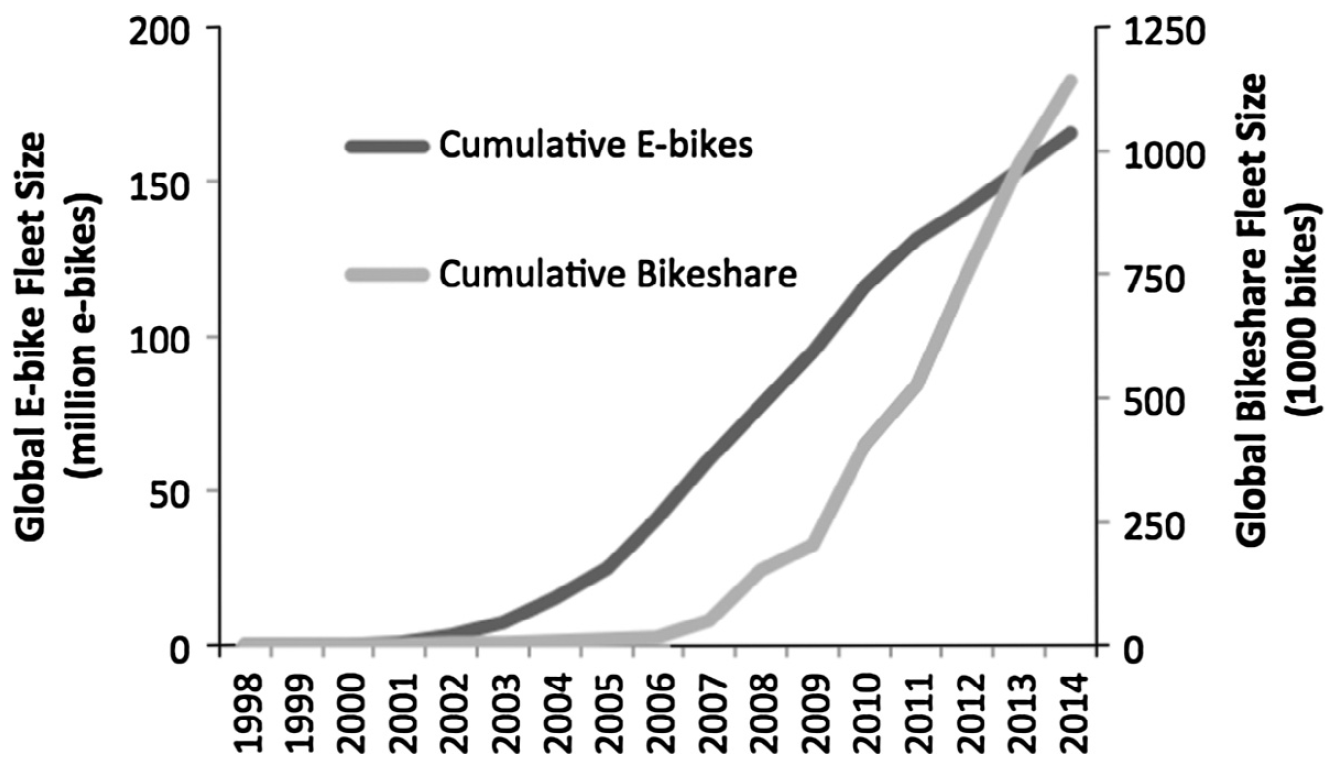
\includegraphics[width=0.6\linewidth]{image/bike_sharing} \caption{Wachstum bei persoenlichen E-Bike- und oeffentlichen Bikeshare-Systemen (Campbell et al., 2016)}\label{fig:unnamed-chunk-55}
\end{figure}

Private FVS-Betreiber aus China (\emph{Mobike, Ofo}) und Shanghai (\emph{oBike}) führen derzeit große Flotten von stationslosen Leihfahrrädern in Städten weltweit ein. Die Einführung, insbesondere in europäischen Städten, ist auf Probleme gestoßen, da die Stadtverwaltungen nicht in der Lage waren, die Einführung zu koordinieren (Zademach und Musch, 2018). Viele Fahrräder wurden in den Städten verlassen aufgefunden. Darüber hinaus wird in einigen Fällen befürchtet, dass die privaten Unternehmen das FVS nur deshalb eingeführt haben, um private Nutzerdaten abzugreifen (Schöffel et al., 2017).
Das Unternehmen Montreal ``BIXI'' hat feste, tragbare, solarbetriebene und modulare Stationen eingeführt. Sie sind in sich geschlossen, und die Stationen können innerhalb von 20 Minuten an den gewünschten Orten aufgestellt, bewegt und verlegt werden. Für besondere Veranstaltungen sind ``Mega''-Dockingstationen erhältlich (Midgley, 2011). Die Zahl der FVS ist auf über 800 Einheiten weltweit angewachsen (Fishman, 2016). Das Modell der öffentlich-privaten Partnerschaft ist am weitesten verbreitet, und die Einführung von FVS war in Städten mit begrenzten öffentlichen Mitteln möglich (Zademach und Musch, 2018).
In Österreich gibt es derzeit mehrere Unternehmen, die Fahrrad- oder E-Bike-Sharing-Dienste anbieten, wie \emph{Citybike, Ofo oder oBike}. Allerdings haben sich die asiatischen Anbieter von stationslosen Leihfahrrädern in Wien (Start-ups \emph{Ofo} und \emph{oBike}) etwa ein Jahr nach ihrem Start aus der Bundeshauptstadt zurückgezogen (Rachbauer, 2018b). Grund dafür sind die strengen Regeln für stationslose Leihfahrräder in Wien, die am 1. August 2018 verkündet wurden. Bei Nichteinhaltung der Regeln wurden die Räder kostenpflichtig entfernt. Bisher erlaubte die Straßenverkehrsordnung (\emph{StVO}) das Aufstellen von Leihfahrrädern im öffentlichen Raum und der Stadt fehlten die Mittel, gegen die Anbieter vorzugehen. Mit Hilfe einer so genannten Ortspolizeiverordnung verlangte das Rathaus von den Bikesharing-Unternehmen, dass sie beanstandete Fahrräder werktags innerhalb von vier Stunden und nachts und am Wochenende innerhalb von zwölf Stunden nach der Benachrichtigung abholen. Wenn sie dem nicht nachkamen, wurden die Fahrräder gegen eine Gebühr entfernt. Darüber hinaus waren Bußgelder von bis zu 700 Euro möglich. Außerdem wurde eine Obergrenze von maximal 1500 Fahrrädern pro Anbieter festgelegt. Jetzt werden die Fahrräder mit einer Nummer versehen und jedes einzelne muss bei der Stadt registriert werden. Die Gründung mehrerer Unternehmen, um die Obergrenze zu umgehen, ist laut Blum nicht erlaubt. Auch die Verleiher selbst müssen bestimmte Kriterien erfüllen, so muss es etwa einen Firmensitz in Wien und eine Service-Hotline geben. Ofo und oBike erfüllen diese Anforderungen bereits (Rachbauer, 2018d).
Österreichweit ist die Situation bei den Leihfahrrädern sehr unterschiedlich, in Innsbruck zum Beispiel wurden 2014 erstmals Leihfahrräder eingeführt und sind erfolgreich in Betrieb. In Linz wurde das Leihradsystem 2017 genehmigt und die Docking-Stationen sind derzeit im Bau. Auch in Salzburg ist das S-Bike Verleihsystem in Betrieb und an eine Bundesförderung gekoppelt (Affenzeller, 2020, Citybike Salzburg, n.d.). In Graz gibt es kein Fahrradverleihsystem. Stattdessen bieten Geschäfte und Hotels einen Verleih an (Rachbauer, 2016).

\hypertarget{relevante-initiativen-in-uxf6sterreich-57}{%
\subsection*{Relevante Initiativen in Österreich}\label{relevante-initiativen-in-uxf6sterreich-57}}
\addcontentsline{toc}{subsection}{Relevante Initiativen in Österreich}

\begin{itemize}
\tightlist
\item
  \href{https://firmenradl.at/cms/}{firmenradl.at}
\item
  \href{https://www.citybikewien.at/de}{citybikewien}
\item
  \href{http://www.citybikesalzburg.at/}{citybikesalzburg}
\item
  \href{https://www.nextbike.at/de/niederoesterreich/}{nextbike}
\item
  \href{https://www.tips.at/nachrichten/linz/land-leute/523512-linzer-radverleih-startet-im-fruehjahr-an-40-standorten}{tpis.at}
\end{itemize}

\hypertarget{auswirkungen-in-bezug-auf-die-ziele-fuxfcr-nachhaltige-entwicklung-sdgs-57}{%
\subsection*{Auswirkungen in Bezug auf die Ziele für nachhaltige Entwicklung (SDGs)}\label{auswirkungen-in-bezug-auf-die-ziele-fuxfcr-nachhaltige-entwicklung-sdgs-57}}
\addcontentsline{toc}{subsection}{Auswirkungen in Bezug auf die Ziele für nachhaltige Entwicklung (SDGs)}

\begin{longtable}[]{@{}ccccc@{}}
\toprule
\begin{minipage}[b]{0.17\columnwidth}\centering
Ebene der Auswirkungen\strut
\end{minipage} & \begin{minipage}[b]{0.16\columnwidth}\centering
Indikator\strut
\end{minipage} & \begin{minipage}[b]{0.17\columnwidth}\centering
Richtung der Auswirkungen\strut
\end{minipage} & \begin{minipage}[b]{0.17\columnwidth}\centering
Beschreibung des Ziels \& SDG\strut
\end{minipage} & \begin{minipage}[b]{0.17\columnwidth}\centering
Quelle\strut
\end{minipage}\tabularnewline
\midrule
\endhead
\begin{minipage}[t]{0.17\columnwidth}\centering
Individuell\strut
\end{minipage} & \begin{minipage}[t]{0.16\columnwidth}\centering
Erhoehte koerperliche Aktivitaet und verbesserte Gesundheit\strut
\end{minipage} & \begin{minipage}[t]{0.17\columnwidth}\centering
\textbf{+}\strut
\end{minipage} & \begin{minipage}[t]{0.17\columnwidth}\centering
Gesundheit und Wohlbefinden (\emph{3})\strut
\end{minipage} & \begin{minipage}[t]{0.17\columnwidth}\centering
Andersen et al., 2009\strut
\end{minipage}\tabularnewline
\begin{minipage}[t]{0.17\columnwidth}\centering
Individuell\strut
\end{minipage} & \begin{minipage}[t]{0.16\columnwidth}\centering
Oft sind die ersten 30-60 Minuten kostenlos\strut
\end{minipage} & \begin{minipage}[t]{0.17\columnwidth}\centering
\textbf{+}\strut
\end{minipage} & \begin{minipage}[t]{0.17\columnwidth}\centering
Gleichheit (\emph{5,10})\strut
\end{minipage} & \begin{minipage}[t]{0.17\columnwidth}\centering
Citybike Salzburg, n.d. b; Citybike Wien, n.d.; Nextbike Niederoesterreich, n.d.\strut
\end{minipage}\tabularnewline
\begin{minipage}[t]{0.17\columnwidth}\centering
Individuell\strut
\end{minipage} & \begin{minipage}[t]{0.16\columnwidth}\centering
Kontinuierliche Weiterentwicklung der Fahrradfunktionen\strut
\end{minipage} & \begin{minipage}[t]{0.17\columnwidth}\centering
\textbf{+}\strut
\end{minipage} & \begin{minipage}[t]{0.17\columnwidth}\centering
Innovation und Infrastruktur (\emph{9})\strut
\end{minipage} & \begin{minipage}[t]{0.17\columnwidth}\centering
Zademach \& Musch, 2018\strut
\end{minipage}\tabularnewline
\begin{minipage}[t]{0.17\columnwidth}\centering
Systemisch\strut
\end{minipage} & \begin{minipage}[t]{0.16\columnwidth}\centering
Breiterer Zugang zu dieser preiswerten oder kostenlosen Mobilitaetsdienstleistung\strut
\end{minipage} & \begin{minipage}[t]{0.17\columnwidth}\centering
\textbf{+}\strut
\end{minipage} & \begin{minipage}[t]{0.17\columnwidth}\centering
Gleichheit (\emph{5,10})\strut
\end{minipage} & \begin{minipage}[t]{0.17\columnwidth}\centering
El Arbi \& Stephane, 2020\strut
\end{minipage}\tabularnewline
\begin{minipage}[t]{0.17\columnwidth}\centering
Systemisch\strut
\end{minipage} & \begin{minipage}[t]{0.16\columnwidth}\centering
Verringerung von Luftverschmutzung, Laermbelaestigung und Verkehrsstaus\strut
\end{minipage} & \begin{minipage}[t]{0.17\columnwidth}\centering
\textbf{+}\strut
\end{minipage} & \begin{minipage}[t]{0.17\columnwidth}\centering
Oekologische Nachhaltigkeit (\emph{7,12,13,15})\strut
\end{minipage} & \begin{minipage}[t]{0.17\columnwidth}\centering
El Arbi \& Stephane, 2020\strut
\end{minipage}\tabularnewline
\begin{minipage}[t]{0.17\columnwidth}\centering
Systemisch\strut
\end{minipage} & \begin{minipage}[t]{0.16\columnwidth}\centering
Investitionen in die Bike-Sharing-Infrastruktur\strut
\end{minipage} & \begin{minipage}[t]{0.17\columnwidth}\centering
\textbf{+}\strut
\end{minipage} & \begin{minipage}[t]{0.17\columnwidth}\centering
Innovation und Infrastruktur (\emph{9})\strut
\end{minipage} & \begin{minipage}[t]{0.17\columnwidth}\centering
der Grazer, 2019; Hillebrand, 2019; Affenzeller, 2020; Tech \& Nature, 2020\strut
\end{minipage}\tabularnewline
\begin{minipage}[t]{0.17\columnwidth}\centering
Systemisch\strut
\end{minipage} & \begin{minipage}[t]{0.16\columnwidth}\centering
48\% aller Systeme werden in oeffentlich-privaten Partnerschaften betrieben\strut
\end{minipage} & \begin{minipage}[t]{0.17\columnwidth}\centering
\textbf{+}\strut
\end{minipage} & \begin{minipage}[t]{0.17\columnwidth}\centering
Partnerschaften und Kooperationen (\emph{17})\strut
\end{minipage} & \begin{minipage}[t]{0.17\columnwidth}\centering
Midgley, 2011\strut
\end{minipage}\tabularnewline
\bottomrule
\end{longtable}

\hypertarget{technologie--und-gesellschaftlicher-bereitschaftsgrad-53}{%
\subsection*{Technologie- und gesellschaftlicher Bereitschaftsgrad}\label{technologie--und-gesellschaftlicher-bereitschaftsgrad-53}}
\addcontentsline{toc}{subsection}{Technologie- und gesellschaftlicher Bereitschaftsgrad}

\begin{longtable}[]{@{}cc@{}}
\toprule
Stand der Technologiebereitschaft & Gesellschaftlicher Bereitschaftsgrad\tabularnewline
\midrule
\endhead
7-9 & 5-7\tabularnewline
\bottomrule
\end{longtable}

\hypertarget{offene-fragen-55}{%
\subsection*{Offene Fragen}\label{offene-fragen-55}}
\addcontentsline{toc}{subsection}{Offene Fragen}

\begin{enumerate}
\def\labelenumi{\arabic{enumi}.}
\tightlist
\item
  Welche Maßnahmen können ergriffen werden, um den Vandalismus an den Verleih-Fahrrädern zu bekämpfen?
\item
  Welches Fahrradsystem (stationsbasiert vs.~stationslos) ist langfristig nachhaltiger?
\end{enumerate}

\hypertarget{weitere-links-46}{%
\subsection*{Weitere links}\label{weitere-links-46}}
\addcontentsline{toc}{subsection}{Weitere links}

\begin{itemize}
\tightlist
\item
  \href{http://en.cyclocity.com/}{cyclocity.com}
\end{itemize}

\hypertarget{referenzen-57}{%
\subsection*{Referenzen}\label{referenzen-57}}
\addcontentsline{toc}{subsection}{Referenzen}

\begin{itemize}
\tightlist
\item
  Affenzeller, J. (2020, December 17). Linzer Radverleih startet im Frühjahr an 40 Standorten. \url{https://www.tips.at/nachrichten/linz/land-leute/523512-linzer-radverleih-startet-im-fruehjahr-an-40-standorten}
\item
  Andersen, L. B., Lawlor, D. A., Cooper, A. R., Froberg, K., and Anderssen, S. A. (2009). Physical fitness in relation to transport to school in adolescents: the Danish youth and sports study. Scandinavian Journal of Medicine \& Science in Sports, 19(3):406-411.
\item
  Campbell, A. A., Cherry, C. R., Ryerson, M. S., \& Yang, X. (2016). Factors influencing the choice of shared bicycles and shared electric bikes in Beijing. Transportation Research Part C: Emerging Technologies, 67, 399--414. \url{https://doi.org/10.1016/j.trc.2016.03.004}
\item
  Cheng, L., Yang, J., Chen, X., Cao, M., Zhou, H., \& Sun, Y. (2020). How could the station-based bike sharing system and the free-floating bike sharing system be coordinated? Journal of Transport Geography, 89(March 2019), 102896. \url{https://doi.org/10.1016/j.jtrangeo.2020.102896}
\item
  Cheng, X., \& Gao, Y. (2018). The Optimal Monthly Strategy Pricing of Free-Floating Bike Sharing Platform. Modern Economy, 09(02), 318--338. \url{https://doi.org/10.4236/me.2018.92021}
\item
  Citybike Salzburg. (n.d.-a). Citybike Salzburg. Available at: \url{http://www.citybikesalzburg.at/hanuschplatz.php} {[}Accessed: 12 January 2021{]}
\item
  Citybike Salzburg. (n.d.-b). Citybike Salzburg - Tarife. Available at: \url{http://www.citybikesalzburg.at/tarife.php} {[}Accessed: 18 January 2021{]}
\item
  Citybike Wien. (n.d.). Tarife - Citybike Wien. Available at: \url{https://www.citybikewien.at/de/tarife} {[}Accessed: 18 January 2021{]}
\item
  Citybike Wien. (2019). 10 Millionen Fahrten bei Citybike Wien! Available at: \url{https://www.citybikewien.at/de/news/595-neuer-meilenstein-bei-citybike-wien-erreicht} {[}Accessed: 17 January 2021{]}
\item
  DeMaio, P. (2009). Bike-sharing: History, Impacts, Models of Provision, and Future. Journal of Public Transportation, 12(4), 41--56. \url{https://doi.org/10.5038/2375-0901.12.4.3}
\item
  der Grazer. (2019, October 21). 100 Millionen Euro für Fahrrad-Offensive im Großraum Graz -- Der Grazer. Available at: \url{https://grazer.at/de/uHAnk5t2/100-millionen-euro-fuer-fahrrad-offensive-im-graz/} {[}Accessed: 17 January 2021{]}
\item
  Eillie, A. (2016). Oxford Test Drives Peer-to-Peer Bike Sharing. \url{https://www.bloomberg.com/news/articles/2016-09-13/cycle-land-is-a-new-peer-to-peer-bike-sharing-platform}
\item
  El Arbi, A. A., \& Stephane, C. K. T. (2020). Intelligent Management of Bike Sharing in Smart Cities using Machine Learning and Internet of Things. Sustainable Cities and Society, 135907. \url{https://doi.org/10.1016/j.scs.2020.102702}
\item
  Fishman, E. (2016). Bikeshare: A Review of Recent Literature. Transport Reviews, 36(1), 92--113. \url{https://doi.org/10.1080/01441647.2015.1033036}
\item
  Fishman, E., Washington, S., Haworth, N., \& Mazzei, A. (2014). Barriers to bikesharing: An analysis from Melbourne and Brisbane. Journal of Transport Geography, 41, 325--337. \url{https://doi.org/10.1016/j.jtrangeo.2014.08.005}
\item
  Gu, T., Kim, I., \& Currie, G. (2019). To be or not to be dockless: Empirical analysis of dockless bikeshare development in China. Transportation Research Part A: Policy and Practice, 119, 122--147. \url{https://doi.org/10.1016/j.tra.2018.11.007}
\item
  Hillebrand, T. (2019). Mietradsystem `Stadtrad Innsbruck' - VCÖ Vorbildhafte Mobilitätsprojekte. Available at: \url{https://mobilitaetsprojekte.vcoe.at/mietradsystem-stadtrad-innsbruck-2019} {[}Accessed: 17 January 2021{]}
\item
  Li, H., Zhang, Y., Ding, H., \& Ren, G. (2019). Effects of dockless bike-sharing systems on the usage of the London Cycle Hire. Transportation Research Part A: Policy and Practice, 130, 398--411. \url{https://doi.org/10.1016/j.tra.2019.09.050}
\item
  Ma, X., Ji, Y., Yuan, Y., Van Oort, N., Jin, Y., \& Hoogendoorn, S. (2020). A comparison in travel patterns and determinants of user demand between docked and dockless bike-sharing systems using multi-sourced data. Transportation Research Part A: Policy and Practice, 139(June), 148--173. \url{https://doi.org/10.1016/j.tra.2020.06.022}
\item
  Midgley, P. (2011). Bicycle-Sharing Schemes: Enhancing Sustainable Mobility in Urban Areas. Commission on Sustainable Development, Nine teent(8), 24. \url{http://www.un.org/esa/dsd/resources/res_pdfs/csd-19/Background-Paper8-P.Midgley-Bicycle.pdf}
\item
  Nextbike Niederösterreich. (n.d.). Nextbike Niederösterreich - Tarife. Available at: \url{https://www.nextbike.at/de/niederoesterreich/preise/} {[}Accessed: 18 January 2021{]}
\item
  Rachbauer, S. (2016, July). Bikesharing in Österreich: Leihräder auf der Überholspur \textbar{} kurier.at. \url{https://kurier.at/chronik/oesterreich/bikesharing-in-oesterreich-leihraeder-auf-der-ueberholspur/400067369}
\item
  Rachbauer, S. (2018a). Bikesharing in Österreich: Leihräder auf der Überholspur. \url{https://kurier.at/chronik/oesterreich/bikesharing-in-oesterreich-leihraeder-auf-der-ueberholspur/400067369}
\item
  Rachbauer, S. (2018b). Leihräder: Wiener wollen es aufgeräumt. \url{https://kurier.at/chronik/wien/leihraeder-wiener-wollen-es-aufgeraeumt/400067357}
\item
  Rachbauer, S. (2018c, March). Wien führt strenge Regeln für stationslose Leihräder ein. \url{https://kurier.at/chronik/wien/wien-fuehrt-strenge-regeln-fuer-stationslose-leihraeder-ein/312.944.617}
\item
  Rachbauer, S. (2018d, July 17). Leihräder: Wiener wollen es aufgeräumt. \url{https://kurier.at/chronik/wien/leihraeder-wiener-wollen-es-aufgeraeumt/400067357}
\item
  Schöffel, R., Zierer, M., \& Kühne, S. (2017). Nutzerdaten offen im Netz: BR deckt Datenleck beim Fahrradverleiher Obike auf. \url{https://www.br.de/nachricht/datenleck-obike-100.html}
\item
  Sun, S., \& Ertz, M. (2021). Contribution of bike-sharing to urban resource conservation: The case of free-floating bike-sharing. Journal of Cleaner Production, 280, 124416. \url{https://doi.org/10.1016/j.jclepro.2020.124416}
\item
  Tech \& Nature. (2020, April 28). Niederösterreich modernisiert Sharing-Bike-Flotte `nextbike' - Tech \& Nature. \url{https://www.techandnature.com/niederosterreich-modernisiert-sharing-bike-flotte-nextbike/}
\item
  Zademach, H. M., \& Musch, A. K. (2018). Bicycle-sharing systems in an alternative/diverse economy perspective: a sympathetic critique. Local Environment, 23(7), 734--746. \url{https://doi.org/10.1080/13549839.2018.1434494}
\item
  Zhang, Y., Lin, D., \& Mi, Z. (2019). Electric fence planning for dockless bike-sharing services. Journal of Cleaner Production, 206, 383--393. \url{https://doi.org/10.1016/j.jclepro.2018.09.215}
\end{itemize}

\hypertarget{scooters}{%
\section{E-Kick-Scooter}\label{scooters}}

\hypertarget{synonyme-50}{%
\subsection*{Synonyme}\label{synonyme-50}}
\addcontentsline{toc}{subsection}{Synonyme}

\emph{Elektroroller}

\hypertarget{definition-58}{%
\subsection*{Definition}\label{definition-58}}
\addcontentsline{toc}{subsection}{Definition}

E-Kick-Scooter sind elektrisch betriebene Roller, die sich, nach einem ersten Abstoßen mit einem Druckhebel beschleunigen lassen und sich danach mit einer ähnlichen Geschwindigkeit wie Fahrräder fortbewegen. Sie sind eine der Lösungen für die Mikromobilität, die in der städtischen Mobilität einen wachsenden Trend darstellt. Sie umfassen alle von Menschen angetriebenen Mikrofahrzeuge wie Fahrräder und Roller, aber auch neue Mikrofahrzeuge wie E-Scooter, E-Bikes und einige andere kleine, elektrisch betriebene Fahrzeuge (Oeschger, Carroll und Caulfield, 2020). Die meisten der modernen Fahrzeuge dieser Art sind sowohl für die gemeinsame als auch für die private Nutzung verfügbar und erfreuen sich einer breiten Akzeptanz. E-Scooter versprechen seit ihrer Einführung im Jahr 2017 eine Lösung für das Problem der letzten Meile (Siegfried et al., 2021). Sie werden als Alternative zum Auto gesehen und bieten das Potenzial, Verkehrsstaus, Lärm und Umweltverschmutzung zu reduzieren. Erste Ergebnisse deuten darauf hin, dass E-Scooter hauptsächlich für Strecken zwischen 1 und 6 km genutzt werden. Empirische Belege zeigen, dass E-Scooter für diese kurzen Strecken eher das Gehen als das Autofahren ersetzen können (James et al., 2019; Portland Bureau of Transportation, 2019). Neben den potenziellen positiven Umweltauswirkungen von E-Scootern auf das Verkehrssystem wurden auch einige Sicherheitsbedenken geäußert. Die meisten E-Scooter-Nutzer, die einen Unfall hatten, fuhren ohne Helm (Liew et al., 2020). Im Allgemeinen werden E-Scooter fast ausschließlich ohne Schutzausrüstung ausgegeben (Allem und Majmundar, 2019). Die Sicherheitsprobleme betreffen nicht nur die Fahrer:innen selbst, sondern haben auch Auswirkungen auf andere Verkehrsteilnehmer:innen, insbesondere Fußgänger:innen (Sikka et al., 2019). Es wurde sogar kritisiert, dass die Technologie dem Konzept ``zuerst verkaufen, dann Sicherheit'' folgt (Choron und Sakran, 2019).

\hypertarget{wichtige-interessensgruppen-58}{%
\subsection*{Wichtige Interessensgruppen}\label{wichtige-interessensgruppen-58}}
\addcontentsline{toc}{subsection}{Wichtige Interessensgruppen}

\begin{itemize}
\tightlist
\item
  \textbf{Betroffene}: Mobile Bürger:innen, Fußgänger:innen, Versicherungen
\item
  \textbf{Verantwortliche}: Nationale Regierungen, Stadtverwaltungen, private Unternehmen
\end{itemize}

\hypertarget{aktueller-stand-der-wissenschaft-und-forschung-58}{%
\subsection*{Aktueller Stand der Wissenschaft und Forschung}\label{aktueller-stand-der-wissenschaft-und-forschung-58}}
\addcontentsline{toc}{subsection}{Aktueller Stand der Wissenschaft und Forschung}

Da es sich bei E-Scootern bereits um eine etablierte Technologie handelt, konzentrieren sich die meisten Forschungsarbeiten auf Sicherheit und Unfälle, das Nutzerverhalten und die potenziellen Umweltauswirkungen der Einführung dieser Mikromobilitätsoption. Einige Studien befürworten E-Scooter als umweltfreundliche Lösung für überfüllte Städte, andere berichten über widersprüchliche Ergebnisse und weisen auf Sicherheitsprobleme hin. Darüber hinaus wird in der Forschung auch untersucht, ob die Präsenz von E-Scootern Fahrraddiebstähle verringert (Gössling, 2020). In Göteborg, Schweden, berichtete die Polizei, dass sich die Zahl der Fahrraddiebstähle nach der Einführung von E-Scootern und Leihfahrrädern halbiert hat (Sydsvenskan, 2019).

\hypertarget{aktueller-stand-der-praktischen-umsetzung-58}{%
\subsection*{Aktueller Stand der praktischen Umsetzung}\label{aktueller-stand-der-praktischen-umsetzung-58}}
\addcontentsline{toc}{subsection}{Aktueller Stand der praktischen Umsetzung}

E-Scooter-Anbieter wie Lime und Bird, die 2017 in Kalifornien den Betrieb aufnahmen, sind inzwischen in über 100 Städten weltweit vertreten und haben seitdem Millionen von Fahrten verzeichnet. Der E-Scooter-Anbieter VOI hat in Europa ein ähnliches Wachstum erlebt und ist nur ein Jahr nach dem Start in Schweden in 10 Ländern auf den Markt gekommen und hat über 16 Millionen Fahrten verzeichnet (Oeschger et al., 2020). Die Ergebnisse einer Umfrage deuten darauf hin, dass E-Scooter in erster Linie als Unterhaltungsgerät und nicht als Transportmittel angesehen werden (Siegfried et al., 2021).
Höchstgeschwindigkeitsbegrenzungen sind ein wichtiges Thema, und international gibt es unterschiedliche Ansätze. In Los Angeles und Dallas gibt es zum Beispiel kein Tempolimit, soweit man das aus den Nachrichten entnehmen kann, während in Wien das Limit bei 25 km/h liegt (Schwarz, 2019). In Paris wird eine Reduzierung der Höchstgeschwindigkeit auf 20 km/h auf Radwegen und 8 km/h in Parks und Fußgängerzonen diskutiert (Négroni, 2019). Ein Problem bei den Höchstgeschwindigkeiten ist, dass einige der E-Scooter-Modelle viel schneller als 25 km/h fahren können (Le Figaro, 2018). Um den negativen Folgen der Einführung von E-Scootern entgegenzuwirken, haben die Städte verschiedene Regeln und Richtlinien evaluiert und umgesetzt. Die Medienanalyse schlägt vor, dass die Stadtverwaltungen folgende Regeln als Mindestanforderung einführen sollten: Geschwindigkeitsbegrenzungen, Beschränkungen für die ausschließliche Nutzung der Fahrradinfrastruktur und eine Ausweisung von Abstellplätzen. Verhaltenskampagnen und Bußgelder sind erforderlich, um die negativen Folgen der E-Scooter-Nutzung zu begrenzen (Gössling, 2020).
In Wien werden nur sehr wenige E-Scooter auf Radwegen benutzt (zwischen 4,9 \% und 7,1 \% im Vergleich zu anderen Radwegbenutzer:innen). In Anbetracht des Modalsplits in Wien (7 \% Radverkehr) kann der Schluss gezogen werden, dass E-Scooter noch keine bedeutende Rolle im Wiener Verkehrssystem spielen (Laa und Leth, 2020).

\hypertarget{relevante-initiativen-in-uxf6sterreich-58}{%
\subsection*{Relevante Initiativen in Österreich}\label{relevante-initiativen-in-uxf6sterreich-58}}
\addcontentsline{toc}{subsection}{Relevante Initiativen in Österreich}

\begin{itemize}
\tightlist
\item
  \href{https://autorevue.at/ratgeber/e-scooter-wien-vergleich}{autorevue.at}
\item
  \href{https://www.stadt-wien.at/wien/news/e-scooter-sharing-system-in-wien.html}{stadt-wien.at}
\item
  \href{https://www.wien.gv.at/verkehr/scooter-roller/index.html}{wien.gv.at}
\item
  \href{https://www.oeamtc.at/thema/fahrrad/e-kleintretroller-e-scooter-in-oesterreich-31721872}{oeamtc.at}
\item
  \href{https://www.oesterreich.gv.at/themen/freizeit_und_strassenverkehr/Elektro-Scooter,-Quads-und-Co/Seite.610110.html}{oesterreich.gv.at}
\end{itemize}

\hypertarget{auswirkungen-in-bezug-auf-die-ziele-fuxfcr-nachhaltige-entwicklung-sdgs-58}{%
\subsection*{Auswirkungen in Bezug auf die Ziele für nachhaltige Entwicklung (SDGs)}\label{auswirkungen-in-bezug-auf-die-ziele-fuxfcr-nachhaltige-entwicklung-sdgs-58}}
\addcontentsline{toc}{subsection}{Auswirkungen in Bezug auf die Ziele für nachhaltige Entwicklung (SDGs)}

\begin{longtable}[]{@{}ccccc@{}}
\toprule
\begin{minipage}[b]{0.17\columnwidth}\centering
Ebene der Auswirkungen\strut
\end{minipage} & \begin{minipage}[b]{0.16\columnwidth}\centering
Indikator\strut
\end{minipage} & \begin{minipage}[b]{0.17\columnwidth}\centering
Richtung der Auswirkungen\strut
\end{minipage} & \begin{minipage}[b]{0.17\columnwidth}\centering
Beschreibung des Ziels \& SDG\strut
\end{minipage} & \begin{minipage}[b]{0.17\columnwidth}\centering
Quelle\strut
\end{minipage}\tabularnewline
\midrule
\endhead
\begin{minipage}[t]{0.17\columnwidth}\centering
Individuell\strut
\end{minipage} & \begin{minipage}[t]{0.16\columnwidth}\centering
E-Scooter-Fahrten ersetzen hauptsaechlich Fusswege\strut
\end{minipage} & \begin{minipage}[t]{0.17\columnwidth}\centering
\textbf{-}\strut
\end{minipage} & \begin{minipage}[t]{0.17\columnwidth}\centering
Gesundheit und Wohlbefinden (\emph{3})\strut
\end{minipage} & \begin{minipage}[t]{0.17\columnwidth}\centering
Laa \& Leth, 2020\strut
\end{minipage}\tabularnewline
\begin{minipage}[t]{0.17\columnwidth}\centering
Individuell\strut
\end{minipage} & \begin{minipage}[t]{0.16\columnwidth}\centering
Teurer im Vergleich zu oeffentlichen Verkehrsmitteln\strut
\end{minipage} & \begin{minipage}[t]{0.17\columnwidth}\centering
\textbf{-}\strut
\end{minipage} & \begin{minipage}[t]{0.17\columnwidth}\centering
Nachhaltige wirtschaftliche Entwicklung (\emph{8,11})\strut
\end{minipage} & \begin{minipage}[t]{0.17\columnwidth}\centering
Widholm, 2021; Wiener Linien, 2021\strut
\end{minipage}\tabularnewline
\begin{minipage}[t]{0.17\columnwidth}\centering
Individuell\strut
\end{minipage} & \begin{minipage}[t]{0.16\columnwidth}\centering
Zunahme der Teilnehmer:innen an der bestehenden Fahrradinfrastruktur\strut
\end{minipage} & \begin{minipage}[t]{0.17\columnwidth}\centering
\textbf{\textasciitilde{}}\strut
\end{minipage} & \begin{minipage}[t]{0.17\columnwidth}\centering
Innovation und Infrastruktur (\emph{9})\strut
\end{minipage} & \begin{minipage}[t]{0.17\columnwidth}\centering
Laa \& Leth, 2020\strut
\end{minipage}\tabularnewline
\begin{minipage}[t]{0.17\columnwidth}\centering
Systemisch\strut
\end{minipage} & \begin{minipage}[t]{0.16\columnwidth}\centering
Hoechster Nutzeranteil sind junge Maenner\strut
\end{minipage} & \begin{minipage}[t]{0.17\columnwidth}\centering
\textbf{-}\strut
\end{minipage} & \begin{minipage}[t]{0.17\columnwidth}\centering
Gleichheit (\emph{5,10})\strut
\end{minipage} & \begin{minipage}[t]{0.17\columnwidth}\centering
Laa \& Leth, 2020\strut
\end{minipage}\tabularnewline
\begin{minipage}[t]{0.17\columnwidth}\centering
Systemisch\strut
\end{minipage} & \begin{minipage}[t]{0.16\columnwidth}\centering
E-Scooter-Fahrten ersetzen nachhaltigere Verkehrsmittel\strut
\end{minipage} & \begin{minipage}[t]{0.17\columnwidth}\centering
\textbf{-}\strut
\end{minipage} & \begin{minipage}[t]{0.17\columnwidth}\centering
Oekologische Nachhaltigkeit (\emph{7,12,13,15})\strut
\end{minipage} & \begin{minipage}[t]{0.17\columnwidth}\centering
Laa \& Leth, 2020\strut
\end{minipage}\tabularnewline
\begin{minipage}[t]{0.17\columnwidth}\centering
Systemisch\strut
\end{minipage} & \begin{minipage}[t]{0.16\columnwidth}\centering
Wachstum im Bereich der Mikromobilitaet\strut
\end{minipage} & \begin{minipage}[t]{0.17\columnwidth}\centering
\textbf{+}\strut
\end{minipage} & \begin{minipage}[t]{0.17\columnwidth}\centering
Nachhaltige wirtschaftliche Entwicklung (\emph{8,11})\strut
\end{minipage} & \begin{minipage}[t]{0.17\columnwidth}\centering
Goessling, 2020\strut
\end{minipage}\tabularnewline
\bottomrule
\end{longtable}

\hypertarget{technologie--und-gesellschaftlicher-bereitschaftsgrad-54}{%
\subsection*{Technologie- und gesellschaftlicher Bereitschaftsgrad}\label{technologie--und-gesellschaftlicher-bereitschaftsgrad-54}}
\addcontentsline{toc}{subsection}{Technologie- und gesellschaftlicher Bereitschaftsgrad}

\begin{longtable}[]{@{}cc@{}}
\toprule
Stand der Technologiebereitschaft & Gesellschaftlicher Bereitschaftsgrad\tabularnewline
\midrule
\endhead
7-9 & 7-9\tabularnewline
\bottomrule
\end{longtable}

\hypertarget{offene-fragen-56}{%
\subsection*{Offene Fragen}\label{offene-fragen-56}}
\addcontentsline{toc}{subsection}{Offene Fragen}

\begin{enumerate}
\def\labelenumi{\arabic{enumi}.}
\tightlist
\item
  Erfordert die zunehmende Präsenz von E-Scootern auf der Fahrradinfrastruktur oder in Fußgängerzonen separate Lösungen für die städtische Straßeninfrastruktur?
\end{enumerate}

\hypertarget{referenzen-58}{%
\subsection*{Referenzen}\label{referenzen-58}}
\addcontentsline{toc}{subsection}{Referenzen}

\begin{itemize}
\tightlist
\item
  Allem, J. P., \& Majmundar, A. (2019). Are electric scooters promoted on social media with safety in mind? A case study on Bird's Instagram. In Preventive Medicine Reports (Vol. 13, pp.~62--63). Elsevier Inc.~\url{https://doi.org/10.1016/j.pmedr.2018.11.013}
\item
  Choron, R. L., \& Sakran, J. V. (2019). The Integration of Electric Scooters: Useful Technology or Public Health Problem? American Journal of Public Health, 109(4), 555--556. \url{https://doi.org/10.2105/AJPH.2019.304955}
\item
  Gössling, S. (2020). Integrating e-scooters in urban transportation: Problems, policies, and the prospect of system change. Transportation Research Part D: Transport and Environment, 79(January), 102230. \url{https://doi.org/10.1016/j.trd.2020.102230}
\item
  James, O., Swiderski, J., Hicks, J., Teoman, D., \& Buehler, R. (2019). Pedestrians and E-Scooters: An Initial Look at E-Scooter Parking and Perceptions by Riders and Non-Riders. Sustainability, 11(20), 5591. \url{https://doi.org/10.3390/su11205591}
\item
  Laa, B., \& Leth, U. (2020). Survey of E-scooter users in Vienna: Who they are and how they ride. Journal of Transport Geography, 89(October), 102874. \url{https://doi.org/10.1016/j.jtrangeo.2020.102874}
\item
  Le Figaro. (2018, September 9). Trottinettes: la mairie de Paris veut une réglementation nationale. \url{https://www.lefigaro.fr/flash-eco/2018/09/09/97002-20180909FILWWW00064-trottinettes-la-mairie-de-paris-veut-une-reglementation-nationale.php}
\item
  Liew, Y. K., Wee, C. P. J., \& Pek, J. H. (2020). New peril on our roads: A retrospective study of electric scooter-related injuries. Singapore Medical Journal, 61(2), 92--95. \url{https://doi.org/10.11622/smedj.2019083}
\item
  Négroni, A. (2019, June 6). Paris: Hidalgo prend des mesures contre les trottinettes électriques. \url{https://www.lefigaro.fr/actualite-france/trottinettes-paris-prend-des-mesures-20190606}
\item
  OECD/ITF. (2020). Safe Micromobility. 98. \url{https://www.itf-oecd.org/safe-micromobility}
\item
  Oeschger, G., Carroll, P., \& Caulfield, B. (2020). Micromobility and public transport integration: The current state of knowledge. Transportation Research Part D: Transport and Environment, 89, 102628. \url{https://doi.org/10.1016/j.trd.2020.102628}
\item
  Portland Bureau of Transportation. (2019). 2018 E-Scooter Findings Report. \url{https://www.portlandoregon.gov/transportation/article/709719\%0Ahttps://trid.trb.org/view/1607260}
\item
  Schwarz, R. (2019, July 27). E-Bikes und E-Scooter sind viel zu schnell! - Ideen-Blog - derStandard.at › Diskurs. \url{https://www.derstandard.at/story/2000106514149/e-bikes-und-e-scooter-sind-viel-zu-schnell}
\item
  Siegfried, C., Martin, B., \& Reichenberger, Y. (2021). Consumer acceptance of shared e-scooters for urban and short-distance mobility. Transportation Research Part D, 91(January), 102680. \url{https://doi.org/10.1016/j.trd.2020.102680}
\item
  Sikka, N., Vila, C., Stratton, M., Ghassemi, M., \& Pourmand, A. (2019). Sharing the sidewalk: A case of E-scooter related pedestrian injury. American Journal of Emergency Medicine, 37(9), 1807.e5-1807.e7. \url{https://doi.org/10.1016/j.ajem.2019.06.017}
\item
  Sydsvenskan. (2019, August 30). Elsparkcyklarna minskar cykelstölderna - Sydsvenskan. Available at: \url{https://www.sydsvenskan.se/2019-08-30/elsparkcyklarna-minskar-cykelstolderna} {[}Accessed: 20 January 2021{]}
\item
  Widholm, K. (n.d.). E-Scooter Sharing-System: Roller von Lime, Tier, Bird und Co.~Available at: \url{https://www.stadt-wien.at/wien/news/e-scooter-sharing-system-in-wien.html} {[}Accessed: 20 January 2021{]}
\item
  Wiener Linien. (n.d.). Übersicht Tickets \textbar{} Tickets \textbar{} Fahrgastinfo \textbar{} Wiener Linien. Available at: \url{https://www.wienerlinien.at/eportal3/ep/channelView.do/pageTypeId/66526/channelId/-46648} {[}Accessed: 20 January 2021{]}
\item
  Zagorskas, J., \& Burinskiene, M. (2020). Challenges caused by increased use of E-powered personal mobility vehicles in European cities. Sustainability (Switzerland), 12(1), 273. \url{https://doi.org/10.3390/su12010273}
\end{itemize}

\hypertarget{ride_hailing}{%
\section{Fahrgemeinschaften (Ride-sharing)}\label{ride_hailing}}

\hypertarget{synonyme-51}{%
\subsection*{Synonyme}\label{synonyme-51}}
\addcontentsline{toc}{subsection}{Synonyme}

\begin{itemize}
\tightlist
\item
  Ride hailing: \emph{Fahrtenvermittlung, App-basierte Fahrdienste, Fahrtenbuchung, Fahrdienste auf Abruf, Transportnetzwerkunternehmen (TNCs), Mobilitätsdienstleister (MSPs - mobility service providers)}
\item
  Ride sharing: \emph{Bildung von Fahrgemeinschaften}
\end{itemize}

\hypertarget{definition-59}{%
\subsection*{Definition}\label{definition-59}}
\addcontentsline{toc}{subsection}{Definition}

Ride-Sharing und Ride-Hailing sind beide aus der ``geteilten Wirtschaft'' oder ``kollaborativen Wirtschaft'' hervorgegangen, die darauf abzielt, nicht ausgelastete Ressourcen gemeinsam zu nutzen, um die Effizienz zu steigern, die Umwelt zu schützen und das Wirtschaftswachstum zu fördern (Tirachini, 2019).

Ride Hailing (RH) ermöglicht die Buchung einer Fahrt über eine Online-Plattform - in der Regel eine App. Die Plattformen bringen Reisende, die eine bestimmte Fahrt buchen möchten, mit anderen Fahrer:innen zusammen, die bereit sind, diese Fahrt im privaten Auto zu übernehmen, basierend auf ihrem Standort. Fahrdienstplattformen machen den Austausch von Bargeld weitgehend überflüssig und wenden grundlegende wirtschaftliche Prinzipien an, um Angebot und Nachfrage durch dynamische Preisanpassungen in Einklang zu bringen. Dieses ursprüngliche Modell ist jedoch nicht in allen Ländern zulässig. In Österreich beispielsweise ist es nicht erlaubt, Ride Hailing mit dem eigenen Auto anzubieten, sondern nur mit Mietwagen. Seit 2021 müssen die Fahrer:innen außerdem einen Wiener Taxiführerschein besitzen (Uber Technologies Inc., n.d.).

Ride-Sharing hingegen beschreibt den Vorgang, bei dem sich ein:e Fahrer:in ein Fahrzeug mit mehreren anderen Fahrern teilt, die in dieselbe Richtung fahren wollen. Einige Unternehmen, die Ride Hailing anbieten, bieten auch Ride-Sharing-Dienste an, wie \emph{UberPool} oder \emph{Lyft Shared}, die in der Regel günstiger und aufgrund der höheren Auslastung auch umweltfreundlicher sind (Herzog, 2018). Dynamische Ridesharing-Systeme verwenden Algorithmen, um Fahrer:innen, die in eine ähnliche Richtung fahren wollen, zusammenzubringen und eine gemeinsame Fahrt zu organisieren (Lokhandwala \& Cai, 2018).

\hypertarget{wichtige-interessensgruppen-59}{%
\subsection*{Wichtige Interessensgruppen}\label{wichtige-interessensgruppen-59}}
\addcontentsline{toc}{subsection}{Wichtige Interessensgruppen}

\begin{itemize}
\tightlist
\item
  \textbf{Betroffene}: Mobile Bürger:innen, Taxifahrer:innen
\item
  \textbf{Verantwortliche}: Nationale Regierungen, Stadtverwaltungen, Privatunternehmen, Verkehrsnetzbetreiber, Softwareanbieter
\end{itemize}

\hypertarget{aktueller-stand-der-wissenschaft-und-forschung-59}{%
\subsection*{Aktueller Stand der Wissenschaft und Forschung}\label{aktueller-stand-der-wissenschaft-und-forschung-59}}
\addcontentsline{toc}{subsection}{Aktueller Stand der Wissenschaft und Forschung}

Obwohl das Ride Hailing aus der Sharing Economy hervorgegangen ist, ist es umstritten, ob es sich letztlich positiv auf die Umwelt ausgewirkt hat (Herzog, 2018).

Jan et al.~(2018) argumentieren, dass Ride Hailing einen positiven Einfluss auf die wirtschaftliche Effizienz hat. Da es den öffentlichen Verkehr sowohl ergänzt als auch mit ihm konkurriert, sind seine Auswirkungen auf die Verkehrsüberlastung in der Nähe von Stadtzentren noch unklar. In Bezug auf die Gleichberechtigung verstärkt das Ride Hailing das Problem der digitalen Kluft und wirft Bedenken hinsichtlich Diskriminierung, Datenschutz und Sicherheit auf. Es ist auch umstritten, ob Prosumenten (Produzenten/Konsumenten) von Sharing-Economy-Plattformen ausgebeutet werden, ob Ride-Hailing-Fahrer angemessen entlohnt werden und wie die Rechte von Arbeitnehmern, die auf Abruf arbeiten, besser geschützt werden können. Auch wenn sich Ride Hailing gerne mit einem grünen Image präsentiert, sind die tatsächlichen Umweltauswirkungen noch nicht gründlich untersucht worden. Jin et al.~(2018) wiesen zudem auf die Gefahr einer begrifflichen Verwirrung in der Ride-Hailing-Forschung hin. Auf der Grundlage der in der Literatur berichteten Belege argumentieren sie, dass es unwahrscheinlich ist, dass Menschen aufgrund von Ride Hailing aufhören, ein Auto zu besitzen.

Alisoltani et al.~(2012) argumentieren, dass Ridesharing die Verkehrsüberlastung reduzieren kann, allerdings nur, wenn die Fahrtendichte hoch ist, was in der Regel in großräumigen Netzwerken der Fall ist. In kleineren Städten mit einem kleinen oder mittelgroßen Netz ist die Fahrtendichte nicht hoch genug. Wichtig ist, dass die Fahrtendichte als die Gesamtzahl der Fahrten (Ausgangs- und Zielorte) innerhalb von 24 Stunden in einem bestimmten Gebiet definiert ist (Miller \& Soberman, 2003).

Lokhandwala \& Cai (2018) verglichen in einer Fallstudie in New York City geteilte automatisierte Fahrzeuge (SAVs) mit traditionellen Taxis und fanden heraus, dass SAVs das Potenzial haben, die Flottengröße in NYC um mehr als 50 \% zu reduzieren und die täglichen Treibhausgasemissionen um bis zu 866 MT CO\textsubscript{2} eq zu verringern.

Die Studie von Martin et al.~(2021) bietet einen aktuellen Überblick über Studien zur Optimierung von Ridesharing. Sie vergleichen verschiedene analytische Ansätze in diesem Forschungsbereich und erörtern das aufkommende Konzept ``agiler'' Algorithmen, die dazu beitragen könnten, die Anforderungen groß angelegter und dynamischer Optimierungsprobleme für Ridesharing zu bewältigen.

Die Nichtregierungsorganisation Mothers Against Drunk Driving (MADD) und Uber - eine der bekanntesten Ride-Hailing-Plattformen - veröffentlichten 2015 einen Bericht, in dem sie auf der Grundlage von Studien in Kalifornien argumentieren, dass das Vorhandensein von Uber-Diensten in einer Stadt die Zahl der Unfälle unter Alkoholeinfluss, an denen jüngere Menschen beteiligt sind, verringern kann. Auf der Grundlage einer Studie über die Daten von Seattle argumentieren sie, dass der Markteintritt von Uber in Seattle mit einem Rückgang der Festnahmen wegen Trunkenheit am Steuer um 10 \% verbunden war.

\hypertarget{aktueller-stand-der-praktischen-umsetzung-59}{%
\subsection*{Aktueller Stand der praktischen Umsetzung}\label{aktueller-stand-der-praktischen-umsetzung-59}}
\addcontentsline{toc}{subsection}{Aktueller Stand der praktischen Umsetzung}

Die beiden bekanntesten Unternehmen, die in den USA Ride Hailing anbieten, sind \emph{Uber} und \emph{Lyft}. Uber zum Beispiel bietet wiederum verschiedene Dienste an, wie zum Beispiel:

\begin{itemize}
\tightlist
\item
  UberX - erschwingliche Fahrten, von Tür zu Tür, ganz für Sie allein
\item
  UberPool - gemeinsame Fahrten, von Tür zu Tür oder mit einem kurzen Fußweg
\item
  UberGreen - nachhaltige Fahrten in Elektrofahrzeugen - und viele mehr.
\end{itemize}

Aufgrund von Vorschriften und Aufständen der lokalen Taxiunternehmen musste Uber sein Geschäftsmodell für europäische Städte anpassen. Andere in West- und Mitteleuropa tätige Ride-Hailing-Plattformen sind \emph{Gett, Bolt, Hailo} oder \emph{Taxilo}. Sie alle unterscheiden sich nur geringfügig und hängen von der Provision ab, die die Fahrer:innen an die jeweilige Plattform zahlen (Khatri, 2020a).

Vor der Covid-19-Pandemie wuchs der Markt für Ride Hailing schnell. Wie andere Branchen auch, brach der Ride-Hailing-Markt im Jahr 2020 aufgrund der Krise und der damit verbundenen Maßnahmen wie Fahrverbote, soziale Distanzierung usw. weltweit ein. Um zu überleben, begannen einige der größeren Unternehmen, wie z. B. Uber, in die On-Demand-Lebensmittel- und Paketzustellung einzusteigen. Es wird erwartet, dass sich die Branche erholen wird, je nachdem, wie schnell sich die allgemeine Wirtschaft von der Krise erholt. Allerdings wird die Geschwindigkeit je nach Land, Region und sozialer Gruppe unterschiedlich sein. Mit Blick auf die Zeit nach der Krise werden die Fahrer:innen von Ride-Hailing-Fahrzeugen verschiedene Sicherheitsmaßnahmen ergreifen müssen, wie z. B. häufige Hygiene, das Tragen von Masken und die Gewährleistung der Rückverfolgbarkeit, um das Vertrauen der Kund:innen zurückzugewinnen. Mushahid Khatri (2021), Chief Executive Officer von \href{https://www.yelowsoft.com/}{Yelowsoft} erwartet, ``dass sich Ride-Hailing-Unternehmen in Richtung Verkehrsbehörden bewegen werden, um Shuttle- und Busdienste auf Abruf anzubieten''. Zweitens ist er der Meinung, dass Ride-Hailing-Unternehmen sicherstellen sollten, dass sie Teil von \protect\hyperlink{maas}{MaaS}) sind (siehe Abschnitt über MaaS) und künstliche Intelligenz (KI) nutzen, um ihre Dienste zu verbessern (Khatri, 2020b).

Die weltweit größte App für Mitfahrgelegenheiten im Fernverkehr ist \emph{BlaBlaCar}, die 90 Millionen Mitglieder hat. Jedes Quartal nutzen 25 Millionen Reisende weltweit BlaBlaCar, um ihre Autofahrt zu organisieren und so die Reisekosten zu teilen (BlaBlaCar, 2021). Ähnlich wie bei anderen Plattformen, die auf der Sharing Economy basieren, wird die Sicherheit durch ein Bewertungssystem gewährleistet, bei dem die Mitfahrer andere Fahrgäste bewerten können und umgekehrt.

Die österreichischen Plattformen \emph{GREENDRIVE} und \emph{Carployee} verbinden Fahrer:innen, die für dieselben Unternehmen oder Institutionen arbeiten, mit dem Ziel, durch gemeinsame Fahrten Firmenparkplätze zu sparen und gleichzeitig die Umwelt zu schützen (GREENDRIVE MOBILITY GMBH, 2020; Carployee, 2020).

\hypertarget{relevante-initiativen-in-uxf6sterreich-59}{%
\subsection*{Relevante Initiativen in Österreich}\label{relevante-initiativen-in-uxf6sterreich-59}}
\addcontentsline{toc}{subsection}{Relevante Initiativen in Österreich}

\begin{itemize}
\tightlist
\item
  \href{https://www.ots.at/presseaussendung/OTS_20210113_OTS0026/free-now-will-als-erste-mobilitaetsplattform-in-europa-bis-2030-null-emissionen-erreichen}{ots.at}
\item
  \href{https://www.umweltberatung.at/carsharing-mitfahrboersen}{umweltberatung.a}
\item
  \href{https://greendrive.at/premium/\#benefits}{greendrive.a}
\item
  \href{https://www.carployee.com/\#start-section}{carployee.com}
\item
  \href{https://ummadum.com/}{ummadum.com}
\end{itemize}

\hypertarget{auswirkungen-in-bezug-auf-die-ziele-fuxfcr-nachhaltige-entwicklung-sdgs-59}{%
\subsection*{Auswirkungen in Bezug auf die Ziele für nachhaltige Entwicklung (SDGs)}\label{auswirkungen-in-bezug-auf-die-ziele-fuxfcr-nachhaltige-entwicklung-sdgs-59}}
\addcontentsline{toc}{subsection}{Auswirkungen in Bezug auf die Ziele für nachhaltige Entwicklung (SDGs)}

\begin{longtable}[]{@{}ccccc@{}}
\toprule
\begin{minipage}[b]{0.17\columnwidth}\centering
Ebene der Auswirkungen\strut
\end{minipage} & \begin{minipage}[b]{0.16\columnwidth}\centering
Indikator\strut
\end{minipage} & \begin{minipage}[b]{0.17\columnwidth}\centering
Richtung der Auswirkungen\strut
\end{minipage} & \begin{minipage}[b]{0.17\columnwidth}\centering
Beschreibung des Ziels \& SDG\strut
\end{minipage} & \begin{minipage}[b]{0.17\columnwidth}\centering
Quelle\strut
\end{minipage}\tabularnewline
\midrule
\endhead
\begin{minipage}[t]{0.17\columnwidth}\centering
Individuell\strut
\end{minipage} & \begin{minipage}[t]{0.16\columnwidth}\centering
Verbesserte Zugaenglichkeit\strut
\end{minipage} & \begin{minipage}[t]{0.17\columnwidth}\centering
\textbf{+}\strut
\end{minipage} & \begin{minipage}[t]{0.17\columnwidth}\centering
Gleichheit (\emph{5,10})\strut
\end{minipage} & \begin{minipage}[t]{0.17\columnwidth}\centering
Abdelwahab, 2020; Tirachini, 2019\strut
\end{minipage}\tabularnewline
\begin{minipage}[t]{0.17\columnwidth}\centering
Systemisch\strut
\end{minipage} & \begin{minipage}[t]{0.16\columnwidth}\centering
Weniger Unfaelle durch betrunkene Fahrer:innen\strut
\end{minipage} & \begin{minipage}[t]{0.17\columnwidth}\centering
\textbf{+}\strut
\end{minipage} & \begin{minipage}[t]{0.17\columnwidth}\centering
Gesundheit und Wohlbefinden (\emph{3})\strut
\end{minipage} & \begin{minipage}[t]{0.17\columnwidth}\centering
Uber \& MADD, 2015\strut
\end{minipage}\tabularnewline
\begin{minipage}[t]{0.17\columnwidth}\centering
Systemisch\strut
\end{minipage} & \begin{minipage}[t]{0.16\columnwidth}\centering
geringere Emissionen pro Kopf\strut
\end{minipage} & \begin{minipage}[t]{0.17\columnwidth}\centering
\textbf{+}\strut
\end{minipage} & \begin{minipage}[t]{0.17\columnwidth}\centering
Oekologische Nachhaltigkeit (\emph{7,12,13,15})\strut
\end{minipage} & \begin{minipage}[t]{0.17\columnwidth}\centering
Tirachini, 2019\strut
\end{minipage}\tabularnewline
\begin{minipage}[t]{0.17\columnwidth}\centering
Systemisch\strut
\end{minipage} & \begin{minipage}[t]{0.16\columnwidth}\centering
Zunahme des motorisierten Verkehrs und der Verkehrsueberlastung; positive Auswirkungen auf die wirtschaftliche Effizienz\strut
\end{minipage} & \begin{minipage}[t]{0.17\columnwidth}\centering
\textbf{\textasciitilde{}}\strut
\end{minipage} & \begin{minipage}[t]{0.17\columnwidth}\centering
Nachhaltige wirtschaftliche Entwicklung (\emph{8,11})\strut
\end{minipage} & \begin{minipage}[t]{0.17\columnwidth}\centering
Tirachini, 2019; Jin et al., 2018\strut
\end{minipage}\tabularnewline
\bottomrule
\end{longtable}

\hypertarget{technologie--und-gesellschaftlicher-bereitschaftsgrad-55}{%
\subsection*{Technologie- und gesellschaftlicher Bereitschaftsgrad}\label{technologie--und-gesellschaftlicher-bereitschaftsgrad-55}}
\addcontentsline{toc}{subsection}{Technologie- und gesellschaftlicher Bereitschaftsgrad}

\begin{longtable}[]{@{}cc@{}}
\toprule
Stand der Technologiebereitschaft & Gesellschaftlicher Bereitschaftsgrad\tabularnewline
\midrule
\endhead
7-9 & 6-9\tabularnewline
\bottomrule
\end{longtable}

\hypertarget{offene-fragen-57}{%
\subsection*{Offene Fragen}\label{offene-fragen-57}}
\addcontentsline{toc}{subsection}{Offene Fragen}

\begin{enumerate}
\def\labelenumi{\arabic{enumi}.}
\tightlist
\item
  Wie können die zunehmenden Bedenken hinsichtlich Diskriminierung, Datenschutz und Sicherheit ausgeräumt werden?
\item
  Welche Auswirkungen des Ride-Hailing auf die Verkehrsüberlastung überwiegen die anderen?
\item
  Wie können die Umweltauswirkungen von Ride-Hailing zuverlässig und ganzheitlich analysiert werden?
\item
  Wie können Ride-Hailing und Ride-Sharing vom privaten Autobesitz abhalten?
\end{enumerate}

\hypertarget{weitere-links-47}{%
\subsection*{Weitere links}\label{weitere-links-47}}
\addcontentsline{toc}{subsection}{Weitere links}

\begin{itemize}
\tightlist
\item
  \href{https://www.ots.at/presseaussendung/OTS_20210113_OTS0026/free-now-will-als-erste-mobilitaetsplattform-in-europa-bis-2030-null-emissionen-erreichen}{ots.at}
\item
  \href{https://www.umweltberatung.at/carsharing-mitfahrboersen}{umweltberatung.at}
\item
  \href{https://greendrive.at/premium/\#benefits}{greendrive}
\item
  \href{https://www.carployee.com/\#start-section}{carployee}
\item
  \href{https://ummadum.com/}{ummadum.com}
\item
  \href{https://www.blablacar.de/}{blablacar}
\item
  \href{https://www.uber.com/at/de/}{uber}
\end{itemize}

\hypertarget{referenzen-59}{%
\subsection*{Referenzen}\label{referenzen-59}}
\addcontentsline{toc}{subsection}{Referenzen}

\begin{itemize}
\tightlist
\item
  Abdelwahab, B. (2020). Ridesharing and Social Inclusion: The Role of Ridesharing in Improving Job Access for Disadvantaged Populations (Doctoral dissertation).
\item
  Alisoltani, N., Leclercq, L., \& Zargayouna, M. (2021). Can dynamic ride-sharing reduce traffic congestion?. Transportation research part B: methodological, 145, 212-246.
\item
  BlaBlaCar. (2021). Über uns - BlaBlaCar. \url{https://blog.blablacar.de/about-us}
\item
  Carployee. (2020). Carployee \textbar{} Für Unternehmen. \url{https://www.carployee.com/}
\item
  GREENDRIVE MOBILITY GMBH. (2020). Greendrive - Premiumpaket für Firmen - Fahrgemeinschaften und Mitfahrgelegenheiten. \url{https://greendrive.at/premium/}
\item
  Herzog, W. (2018, October 18). Ecolane Blog: Ride-hailing vs.~ride-sharing: The key difference and why it matters. \url{https://www.ecolane.com/blog/ride-hailing-vs.-ride-sharing-the-key-difference-and-why-it-matters}
\item
  Jin, S. T., Kong, H., Wu, R., \& Sui, D. Z. (2018). Ridesourcing, the sharing economy, and the future of cities. Cities, 76, 96-104.
\item
  Khatri, M. (2020a). A closer look at the ride-hailing landscape of the Western and Central Europe. \url{https://www.yelowsoft.com/blog/ride-hailing-landscape-of-western-and-central-europe/}
\item
  Khatri, M. (2020b). Ride-hailing in 2021: A glimpse into the future. Available at: \url{https://www.yelowsoft.com/blog/ride-hailing-a-glimpse-into-the-future/} {[}Accessed: 30 March 2021{]}
\item
  Lokhandwala, M., \& Cai, H. (2018). Dynamic ride sharing using traditional taxis and shared autonomous taxis: A case study of NYC. Transportation Research Part C: Emerging Technologies, 97, 45-60.
\item
  Martins, L. D. C., de la Torre, R., Corlu, C. G., Juan, A. A., \& Masmoudi, M. A. (2021). Optimizing ride-sharing operations in smart sustainable cities: Challenges and the need for agile algorithms. Computers \& Industrial Engineering, 153, 107080.
\item
  Miller, E., \& Soberman, R. (2003). Travel Demand.
\item
  Tirachini, A. (2019). Ride-hailing, travel behaviour and sustainable mobility: an international review. Transportation, 1-37.
\item
  Uber Technologies Inc.~(n.d.). Erhalte eine Konzession in Österreich. Available at: \url{https://www.uber.com/at/de/drive/requirements/get-a-license/} {[}Accessed: 30 March 2021{]}
\item
  Uber, \& Mothers Against Drunk Driving (MADD). (2015). MORE OPTIONS. SHIFTING MINDSETS. DRIVING BETTER CHOICES. \#ThinkandRide.
\end{itemize}

\hypertarget{passenger_drones}{%
\section{Passagierdrohnen}\label{passenger_drones}}

\hypertarget{synonyme-52}{%
\subsection*{Synonyme}\label{synonyme-52}}
\addcontentsline{toc}{subsection}{Synonyme}

\emph{urbane Luftmobilität (UAM- urban air mobility), vertikale Starts und Landungen (VTOL - vertical take-off and landing), unbemannte Luftfahrzeuge (UAVs - unmanned aerial vehicles)}

\hypertarget{definition-60}{%
\subsection*{Definition}\label{definition-60}}
\addcontentsline{toc}{subsection}{Definition}

Drohnen oder unbemannte Luftfahrzeuge (UAVs) könnten die ikonischste Technologie des 21. Jahrhunderts werden. Drohnen vereinen drei Schlüsselprinzipien der technologischen Moderne: Datenverarbeitung, Automatisierung und grenzenlose Mobilität. Fähigkeiten, die bisher nur vom Militär genutzt werden konnten, werden nun für den größten Teil der Bevölkerung zugänglich. Die potenziellen Anwendungsfälle für Drohnen reichen von Überwachungs- und Aufklärungsmissionen bis hin zu neuartigen Formen der Logistik und des Personentransports. Die kommerzielle Nutzung von Drohnen ist mit enormen wirtschaftlichen Chancen verbunden. Doch auch wenn Drohnen als Überwachungs- und Erfassungsgeräte in Sicherheitsdiensten, in der Geodäsie oder in der Landwirtschaft bereits weit verbreitet sind, steht ihre Nutzung als Transportmittel noch am Anfang (Kellermann et al., 2020).
Lieferdrohnen sind derzeit in der Lage, Gewichte von bis zu 2-3 kg zu heben und Flugmissionen im städtischen Raum durchzuführen (Kellermann et al., 2020). Auch Passagierdrohnen haben bereits die technische Fähigkeit bewiesen, Passagiere innerhalb oder zwischen Städten zu transportieren (LeBeau, 2016; Holt, 2018; Hawkins, 2018). Dies ist nicht nur ein historischer Wendepunkt in der Luftfahrt, sondern auch der Beginn einer neuen Ära, in der sich der flache Luftraum zur ``dritten Dimension'' des Verkehrs entwickeln könnte (Kellermann et al., 2020).
Der Name des neuen Fahrzeugtyps ist noch weit davon entfernt, international vereinbart zu werden. Zur Auswahl stehen mehrere Namen wie Passagierdrohne, bemannter Multikopter, Passenger Air Vehicle (PAV), Electric Vertical Take-off and Landing Aircraft (EVTOL), automatisierte Lufttaxis, unbemannte Lufttaxis, fliegende Autos oder auch noch weitere neue Begriffe (Pramer \& Sommavilla, 2020).
Die automatisierten Lufttaxis werden eine Mischung aus Hubschrauber und Drohne sein. Das bedeutet aber auch, dass es sich um senkrecht startende und landende (VTOL) Fahrzeuge handeln wird. Es gibt mehrere Gründe, warum die Drohnenindustrie stark gefördert wird. Einer der Gründe ist, dass der Luftraum noch relativ frei von Verkehr ist. Die Gefahr von Kollisionen ist (relativ) gering und Autopiloten für Flugzeuge haben sich längst etabliert. Branchenexperten vermuten daher, dass wir selbstfliegende Lufttaxis noch vor selbstfahrenden Autos sehen könnten. Der Verzicht auf Piloten würde einen Lufttaxidienst noch billiger machen und es mehr Menschen ermöglichen, ihn sich zu leisten (UNIQA, 2019).
Die Europäische Kommission schätzt die wirtschaftlichen Auswirkungen bis 2035 auf jährlich 10 Milliarden Euro und rechnet mit der Schaffung von mehr als 100.000 direkten Arbeitsplätzen. Unter Berücksichtigung der indirekten makroökonomischen Auswirkungen in den mit Drohnen verbundenen Branchen rechnet die Kommission sogar mit 250.000 bis 400.000 zusätzlichen Arbeitsplätzen (SESAR, 2016).

\hypertarget{wichtige-interessensgruppen-60}{%
\subsection*{Wichtige Interessensgruppen}\label{wichtige-interessensgruppen-60}}
\addcontentsline{toc}{subsection}{Wichtige Interessensgruppen}

\begin{itemize}
\tightlist
\item
  \textbf{Betroffene}: Bürger:innen, Versicherungen
\item
  \textbf{Verantwortliche}: Nationale Regierungen, Stadtverwaltungen, Privatunternehmen
\end{itemize}

\hypertarget{aktueller-stand-der-wissenschaft-und-forschung-60}{%
\subsection*{Aktueller Stand der Wissenschaft und Forschung}\label{aktueller-stand-der-wissenschaft-und-forschung-60}}
\addcontentsline{toc}{subsection}{Aktueller Stand der Wissenschaft und Forschung}

Da alle Prototypen im Besitz privater Unternehmen sind und die Technologie aufgrund des Wettbewerbs nicht wirklich geteilt wird, gibt es nur wenige technische Forschungsarbeiten. Die Medienanalyse über Drohnen für den Paket- und Personentransport zeigt, dass sich die Forschung derzeit auf die folgenden Bereiche konzentriert (siehe Tabelle unten):

\begin{longtable}[]{@{}ccc@{}}
\toprule
Themen & Prozentsatz & Anzahl der Studien\tabularnewline
\midrule
\endhead
Allgemeine Erhebungen & 18.9\% & 21\tabularnewline
Logistik (allgemein) & 18.0\% & 20\tabularnewline
Einstellungs- und Akzeptanzforschung & 13.5\% & 15\tabularnewline
Recht und Vorschriften & 11.7\% & 13\tabularnewline
Ethik und Technikfolgenabschaetzung & 10.8\% & 12\tabularnewline
Bewertung der Nachhaltigkeit & 8.1\% & 9\tabularnewline
Stadt- und Verkehrsplanung & 7.2\% & 8\tabularnewline
Politische Agenda/Strategien & 6.3\% & 7\tabularnewline
Personenbefoerderung & 2.7\% & 3\tabularnewline
Humanitaere Logistik & 2.7\% & 3\tabularnewline
\bottomrule
\end{longtable}

Und obwohl es derzeit noch keine automatisierten Lufttaxis gibt, gibt es eine erste Studie, die die Faktoren für die Bereitschaft der Nutzer:innen untersucht, mit automatisierten Lufttaxis zu fliegen. In dieser Studie wurden vier Faktoren ermittelt, die sich als signifikant positiv erwiesen: Vertrautheit, Nutzen, Spaßfaktor, Glücksgefühl und zwei als signifikant negativ: Abneigung gegen neue Technologien und Angst (Winter et al., 2020).
Vergleicht man die THG-Emissionen herkömmlicher Autos mit denen von VTOL-Passagierdrohnen, so schneidet die Passagierdrohne ab 35 km tatsächlich etwas besser ab als ein normales Auto. Die Gründe für diesen Break-even-Punkt sind einerseits der energieintensive Start- und Landemodus im Schwebeflug und andererseits die enorme Effizienz des Fluges von Punkt A nach Punkt B. Angesichts der erwarteten erheblichen Zeitersparnis gegenüber dem Auto fahren könnten Passagiere einen Anreiz haben, VTOL-Reisen zu teilen. Daher scheint es wahrscheinlich, dass die durchschnittliche Auslastung von VTOLs größer sein wird als die von herkömmlichen Pkw (Kasliwal et al., 2019).

\hypertarget{aktueller-stand-der-praktischen-umsetzung-60}{%
\subsection*{Aktueller Stand der praktischen Umsetzung}\label{aktueller-stand-der-praktischen-umsetzung-60}}
\addcontentsline{toc}{subsection}{Aktueller Stand der praktischen Umsetzung}

An der Entwicklung der unbemannten Lufttaxis arbeiten bereits mehrere Anbieter Das Münchner Start-up \emph{Lilium} hat Anfang Mai 2019 einen anderthalb Tonnen schweren Prototyp erfolgreich vertikal in die Luft steigen lassen und in der Schwebe gehalten. Er klingt wie ein Hubschrauber, sieht aber nicht so aus: Der Lilium Jet hat Tragflächen und 36 vollelektrische Düsenmotoren. Dadurch ist er leiser und energieeffizienter (und sieht futuristischer aus) als ein Hubschrauber. Lilium geht davon aus, dass der kommerzielle Alltagsbetrieb nicht vor 2025 aufgenommen werden kann.
Aber \emph{Lilium} ist bei weitem nicht der einzige Hersteller. \emph{Joby Aviation, Volocopter, AeroMobil, Kittyhawk} und \emph{Zee.Aero} sind nur einige der Unternehmen, die darauf hoffen, das erfolgreichste Modell auf den Markt zu bringen. Auch bereits etablierte Unternehmen nehmen das Konzept sehr ernst. Das Mobilitätsunternehmen Uber, die Flugzeughersteller \emph{Airbus} und \emph{Boeing} sowie Autofirmen wie \emph{Daimler} und \emph{Porsche} sind im Rennen (UNIQA, 2019). Einige Hersteller wie Boeing (LeBeau, 2016), Airbus (Hawkins, 2018) und Volocopter (Holt, 2018) haben bereits die ersten Flugtests ihrer Prototypen durchgeführt.
Die Europäische Union schlägt vor, dass Unterstützungsdienste wie Flugplanung, Fluggenehmigungen und -freigaben sowie dynamische Luftrauminformationen ab 2022 für den Drohnenflug zur Verfügung stehen sollen. Ab 2027 werden Dienste wie Kollisionsvermeidung und Kapazitätsmanagement in überlasteten Gebieten folgen. Ab 2035, so der Zeitplan der Europäischen Kommission, soll die vollständige Integration von unbemannten Luftfahrzeugen in den kontrollierten Luftraum mit der bemannten Luftfahrt abgeschlossen sein (Wiener Zeitung, 2019).
Das Lufttaxi wird in den nächsten zehn Jahren keine Touristenmassen befördern, aber dank des sinkenden Geräuschpegels der Rotoren, die im ``normalen Stadtlärm'', wie Volocopter behauptet, nicht mehr wahrnehmbar sind, werden sie in der einen oder anderen Millionenmetropole immer öfter zum Einsatz kommen (Pramer \& Sommavilla, 2020).

Die erste genehmigte Teststrecke in Österreich für ein unbemanntes Lufttaxi befindet sich in Linz. In Österreich gibt es bereits einen funktionierenden Prototyp, der von \emph{Ehang} in China entwickelt und von \emph{FACC} im Innviertel gebaut wurde. Das Flugzeug kostet rund 300.000 Euro, wiegt 360 Kilo, ist mit 16 Elektromotoren und 16 Rotoren ausgestattet und soll zwei Personen vollständig automatisiert transportieren. Die Batterien der achtarmigen Drohne reichen für rund 50 Kilometer. In einer eigenen Produktionslinie in Ried sollen bis Ende nächsten Jahres 300 Stück ausgeliefert werden. Damit sie in Europa und auch für die Linz AG abheben können, arbeitet man mit der Austro Control an den ``Zulassungsbestimmungen'', erklärt FACC-Vorstand Robert Machtlinger. In Linz wurde noch einmal betont, dass diese Art der Personenbeförderung als Ergänzung zu Bus und Bahn gesehen wird. Die Luft ermöglicht in Ballungsräumen die schnellste Verbindung von A nach B. Bevor jedoch in der oberösterreichischen Landeshauptstadt die erste Teststrecke für diesen automatisierten Verkehr eingerichtet wird, muss zunächst der 5G-Mobilfunk installiert werden, was für das Frühjahr 2020 geplant war (DerStandard, 2019).

\hypertarget{relevante-initiativen-in-uxf6sterreich-60}{%
\subsection*{Relevante Initiativen in Österreich}\label{relevante-initiativen-in-uxf6sterreich-60}}
\addcontentsline{toc}{subsection}{Relevante Initiativen in Österreich}

\begin{itemize}
\tightlist
\item
  \href{https://www.derbrutkasten.com/autonome-lufttaxis-linz-ag-facc-ehang/}{derbrutkasten.com}
\item
  \href{https://www.derstandard.at/story/2000103120464/erste-teststrecke-fuer-e-lufttaxis-2020-in-linz}{derstandard.at-1}
\item
  \href{https://www.derstandard.at/story/2000122402408/flugtaxis-wann-kommt-der-tesla-der-luefte}{derstandard.at-2}
\end{itemize}

\hypertarget{auswirkungen-in-bezug-auf-die-ziele-fuxfcr-nachhaltige-entwicklung-sdgs-60}{%
\subsection*{Auswirkungen in Bezug auf die Ziele für nachhaltige Entwicklung (SDGs)}\label{auswirkungen-in-bezug-auf-die-ziele-fuxfcr-nachhaltige-entwicklung-sdgs-60}}
\addcontentsline{toc}{subsection}{Auswirkungen in Bezug auf die Ziele für nachhaltige Entwicklung (SDGs)}

\begin{longtable}[]{@{}ccccc@{}}
\toprule
\begin{minipage}[b]{0.17\columnwidth}\centering
Ebene der Auswirkungen\strut
\end{minipage} & \begin{minipage}[b]{0.16\columnwidth}\centering
Indikator\strut
\end{minipage} & \begin{minipage}[b]{0.17\columnwidth}\centering
Richtung der Auswirkungen\strut
\end{minipage} & \begin{minipage}[b]{0.17\columnwidth}\centering
Beschreibung des Ziels \& SDG\strut
\end{minipage} & \begin{minipage}[b]{0.17\columnwidth}\centering
Quelle\strut
\end{minipage}\tabularnewline
\midrule
\endhead
\begin{minipage}[t]{0.17\columnwidth}\centering
Individuell\strut
\end{minipage} & \begin{minipage}[t]{0.16\columnwidth}\centering
erhebliche Zeitersparnis\strut
\end{minipage} & \begin{minipage}[t]{0.17\columnwidth}\centering
\textbf{+}\strut
\end{minipage} & \begin{minipage}[t]{0.17\columnwidth}\centering
Gesundheit und Wohlbefinden (\emph{3})\strut
\end{minipage} & \begin{minipage}[t]{0.17\columnwidth}\centering
Kasliwal et al., 2019\strut
\end{minipage}\tabularnewline
\begin{minipage}[t]{0.17\columnwidth}\centering
Individuell\strut
\end{minipage} & \begin{minipage}[t]{0.16\columnwidth}\centering
Fuer den allgemeinen Gebrauch duerfte es zu kostspielig sein\strut
\end{minipage} & \begin{minipage}[t]{0.17\columnwidth}\centering
\textbf{-}\strut
\end{minipage} & \begin{minipage}[t]{0.17\columnwidth}\centering
Gleichheit (\emph{5,10})\strut
\end{minipage} & \begin{minipage}[t]{0.17\columnwidth}\centering
Pramer \& Sommavilla, 2020\strut
\end{minipage}\tabularnewline
\begin{minipage}[t]{0.17\columnwidth}\centering
Individuell\strut
\end{minipage} & \begin{minipage}[t]{0.16\columnwidth}\centering
Der Flugpreis wird sich voraussichtlich im Bereich eines sehr teuren Taxis einpendeln\strut
\end{minipage} & \begin{minipage}[t]{0.17\columnwidth}\centering
\textbf{-}\strut
\end{minipage} & \begin{minipage}[t]{0.17\columnwidth}\centering
Nachhaltige wirtschaftliche Entwicklung (\emph{8,11})\strut
\end{minipage} & \begin{minipage}[t]{0.17\columnwidth}\centering
Pramer \& Sommavilla, 2020\strut
\end{minipage}\tabularnewline
\begin{minipage}[t]{0.17\columnwidth}\centering
Systemisch\strut
\end{minipage} & \begin{minipage}[t]{0.16\columnwidth}\centering
Leicht verringerte Treibhausgasemissionen im Vergleich zu herkoemmlichen Autos ab 35 km\strut
\end{minipage} & \begin{minipage}[t]{0.17\columnwidth}\centering
\textbf{\textasciitilde{}}\strut
\end{minipage} & \begin{minipage}[t]{0.17\columnwidth}\centering
Oekologische Nachhaltigkeit (\emph{7,12,13,15})\strut
\end{minipage} & \begin{minipage}[t]{0.17\columnwidth}\centering
Kasliwal et al., 2019\strut
\end{minipage}\tabularnewline
\begin{minipage}[t]{0.17\columnwidth}\centering
Systemisch\strut
\end{minipage} & \begin{minipage}[t]{0.16\columnwidth}\centering
Hoehere Investitionen bis 2035 und Schaffung von Arbeitsplaetzen\strut
\end{minipage} & \begin{minipage}[t]{0.17\columnwidth}\centering
\textbf{+}\strut
\end{minipage} & \begin{minipage}[t]{0.17\columnwidth}\centering
Nachhaltige wirtschaftliche Entwicklung (\emph{8,11})\strut
\end{minipage} & \begin{minipage}[t]{0.17\columnwidth}\centering
SESAR, 2016\strut
\end{minipage}\tabularnewline
\begin{minipage}[t]{0.17\columnwidth}\centering
Systemisch\strut
\end{minipage} & \begin{minipage}[t]{0.16\columnwidth}\centering
Stationaere Bereiche fuer Sicherheitskontrollen\strut
\end{minipage} & \begin{minipage}[t]{0.17\columnwidth}\centering
\textbf{\textasciitilde{}}\strut
\end{minipage} & \begin{minipage}[t]{0.17\columnwidth}\centering
Innovation und Infrastruktur (\emph{9})\strut
\end{minipage} & \begin{minipage}[t]{0.17\columnwidth}\centering
Pramer \& Sommavilla, 2020\strut
\end{minipage}\tabularnewline
\bottomrule
\end{longtable}

\hypertarget{technologie--und-gesellschaftlicher-bereitschaftsgrad-56}{%
\subsection*{Technologie- und gesellschaftlicher Bereitschaftsgrad}\label{technologie--und-gesellschaftlicher-bereitschaftsgrad-56}}
\addcontentsline{toc}{subsection}{Technologie- und gesellschaftlicher Bereitschaftsgrad}

\begin{longtable}[]{@{}cc@{}}
\toprule
Stand der Technologiebereitschaft & Gesellschaftlicher Bereitschaftsgrad\tabularnewline
\midrule
\endhead
5-6 & 1-3\tabularnewline
\bottomrule
\end{longtable}

\hypertarget{offene-fragen-58}{%
\subsection*{Offene Fragen}\label{offene-fragen-58}}
\addcontentsline{toc}{subsection}{Offene Fragen}

\begin{enumerate}
\def\labelenumi{\arabic{enumi}.}
\tightlist
\item
  Wer wird die Vorschriften für Passagierdrohnen entwickeln?
\item
  Wie viel Platz wird zum Starten und Landen benötigt, und wird sich dieser zwischen den verschiedenen Anbietern unterscheiden?
\item
  Welche Arten von Strecken werden durch fliegende Taxis ersetzt werden?
\item
  Werden einige Unternehmen zusammenarbeiten und ihre Technologien gemeinsam nutzen?
\item
  Welche weiteren Anwendungsbereiche wird es geben?
\item
  Welches sind die thematischen Entwicklungsschwerpunkte der nächsten Jahre?
\item
  Auf welchen Namen wird man sich international für diese Art von Fahrzeugen einigen?
\end{enumerate}

\hypertarget{referenzen-60}{%
\subsection*{Referenzen}\label{referenzen-60}}
\addcontentsline{toc}{subsection}{Referenzen}

\begin{itemize}
\tightlist
\item
  DerStandard. (2019, May 14). Teststrecke: Erstes unbemanntes Lufttaxi hebt 2020 in Linz ab - Unternehmen - derStandard.at › Wirtschaft. \url{https://www.derstandard.at/story/2000103120464/erste-teststrecke-fuer-e-lufttaxis-2020-in-linz}
\item
  Holt, K. (2018, October 24). Volocopter will test its autonomous air taxis in Singapore next year \textbar{} Engadget. \url{https://www.engadget.com/2018-10-24-volocopter-air-taxi-test-singapore-autonomous-drone-helicopter.html}
\item
  J. Hawkins, A. (2018, February 1). Airbus' autonomous `air taxi' Vahana completes its first test flight - The Verge. \url{https://www.theverge.com/2018/2/1/16961688/airbus-vahana-evtol-first-test-flight}
\item
  Kasliwal, A., Furbush, N. J., Gawron, J. H., McBride, J. R., Wallington, T. J., De Kleine, R. D., Kim, H. C., \& Keoleian, G. A. (2019). Role of flying cars in sustainable mobility. Nature Communications, 10(1). \url{https://doi.org/10.1038/s41467-019-09426-0}
\item
  Kellermann, R., Biehle, T., \& Fischer, L. (2020). Drones for parcel and passenger transportation: A literature review. Transportation Research Interdisciplinary Perspectives, 4, 100088. \url{https://doi.org/10.1016/j.trip.2019.100088}
\item
  LeBeau, P. (2016, January 23). Boeing's first test flight of air taxi a success as it works on Uber Air. \url{https://www.cnbc.com/2019/01/23/boeing-takes-step-in-developing-uber-air--with-successful-test-flight.html}
\item
  Pramer, P., \& Sommavilla, F. (2020, December 11). Flugtaxis: Wann kommt der Tesla der Lüfte? - PodcastEditionZukunft - derStandard.at › EditionZukunft. \url{https://www.derstandard.at/story/2000122402408/flugtaxis-wann-kommt-der-tesla-der-luefte}
\item
  SESAR. (2016). European Drones Outlook Study. In Single European Sky ATM Research (Issue November). \url{https://doi.org/10.2829/219851}
\item
  UNIQA. (2019, October 24). Lufttaxis: Die Überflieger im Verkehr \textbar{} UNIQA Österreich \textbar{} UNIQA Österreich. \url{https://www.uniqa.at/versicherung/mobilitaet/lufttaxis.html}
\item
  Wiener Zeitung. (2019, September 20). Regelwerk für autonome Lufttaxis noch offen - Wiener Zeitung Online. \url{https://www.wienerzeitung.at/nachrichten/wirtschaft/oesterreich/2030182-Fliegen-statt-fahren.html}
\item
  Winter, S. R., Rice, S., \& Lamb, T. L. (2020). A prediction model of Consumer's willingness to fly in autonomous air taxis. Journal of Air Transport Management, 89(August), 101926. \url{https://doi.org/10.1016/j.jairtraman.2020.101926}
\end{itemize}

\hypertarget{alternative}{%
\chapter{Alternative Energieträger}\label{alternative}}

\hypertarget{FCEV}{%
\section{Wasserstoff-Brennstoffzelle}\label{FCEV}}

\hypertarget{synonyme-53}{%
\subsection*{Synonyme}\label{synonyme-53}}
\addcontentsline{toc}{subsection}{Synonyme}

\emph{Wasserstoff-Brennstoffzellen-Elektrofahrzeuge (FCEV - fuel cell electric vehicles)}

\hypertarget{definition-61}{%
\subsection*{Definition}\label{definition-61}}
\addcontentsline{toc}{subsection}{Definition}

Wasserstoff-Brennstoffzellen sind Systeme, die Wasserstoff als Kraftstoff verwenden, um in einer Brennstoffzelle elektrische Energie zu erzeugen und das Fahrzeug mit dieser anzutreiben. In technischer Hinsicht weisen sie Ähnlichkeiten mit Elektrofahrzeugen auf. Die Vorteile von Brennstoffzellen-Elektrofahrzeugen (FCEV) sind Emissionsfreiheit (nur Wasser), schnelle Betankung, geräuschloses Fahren, sparsamerer Kraftstoffverbrauch und Effizienz sowie einfache Wartung. Unabhängig von diesen Vorteilen haben FCEV einige Nachteile, wie z. B. begrenzte Reichweite, Mangel an Wasserstofftankstellen, Sicherheitsprobleme, geringe Rentabilität für die Automobilhersteller, hohe Preise und geringes Bewusstsein und Akzeptanz (Tanç et al., 2019; Borgstedt et al., 2017; Iribarren et al., 2016). FCEVs haben jedoch eine höhere Energiedichte als Elektrobatterien, so dass sie auch mit schwereren Lasten fahren können. Gleichzeitig ergeben sich dadurch Einschränkungen in Bezug auf Gewicht und Größe der Energiespeicher in den Fahrzeugen. Folglich eignen sich FCEVs besser für den Güterverkehr, Nutzfahrzeuge, Busse, Züge, Schiffe und Flugzeuge, wo die Leistungsanforderungen höher sind. Von allen genannten Beispielen gibt es bereits Prototypen (Eichlseder et al, 2018). Bei Privatfahrzeugen dürften die FCEVs bei Langstreckenfahrten Vorteile bieten (Roadmap Europe, 2019).

\hypertarget{wichtige-interessensgruppen-61}{%
\subsection*{Wichtige Interessensgruppen}\label{wichtige-interessensgruppen-61}}
\addcontentsline{toc}{subsection}{Wichtige Interessensgruppen}

\begin{itemize}
\tightlist
\item
  \textbf{Betroffene}: Fahrer:innen von konventionellen Autos, Bürger:innen
\item
  \textbf{Verantwortliche}: Nationale Regierungen, Autohersteller, internationale Lobbyisten, Privatunternehmen
\end{itemize}

\hypertarget{aktueller-stand-der-wissenschaft-und-forschung-61}{%
\subsection*{Aktueller Stand der Wissenschaft und Forschung}\label{aktueller-stand-der-wissenschaft-und-forschung-61}}
\addcontentsline{toc}{subsection}{Aktueller Stand der Wissenschaft und Forschung}

Das Ziel alternativer Antriebssysteme ist es, die klimaschädlichen CO\textsubscript{2}-Emissionen zu minimieren oder ganz zu eliminieren, weshalb das Forschungsprogramm der Europäischen Gemeinschaft die Elektromobilität als vorrangigen Forschungsbereich vorschlägt. Die Methoden der Wasserstofferzeugung durch biologische und photochemische Verfahren werden jedoch auch intensiv erforscht, denn 95 \% des derzeit industriell erzeugten Wasserstoffs stammen aus fossilen Kohlenwasserstoffen und nur 5 \% aus Wasser durch Elektrolyse. Das einzige emissionsfreie Verfahren zur Herstellung von Wasserstoff ist die elektrochemische Wasserspaltung in der Elektrolyse, bei der der benötigte Strom aus Wind-, Wasser- oder Sonnenenergie gewonnen wird. Dieses Verfahren führt zu hohen Reinheitsgraden und erreicht in der Regel Wirkungsgrade von bis zu 85 \% (Eichlseder et al., 2018). Darüber hinaus zielt die Politik für Elektrofahrzeuge auf die Optimierung von Technologie, Marktentwicklung, Haltbarkeit und Kapazität der Batterien und Ladestationen ab (Alvarez-Meaza et al., 2020).

\hypertarget{aktueller-stand-der-praktischen-umsetzung-61}{%
\subsection*{Aktueller Stand der praktischen Umsetzung}\label{aktueller-stand-der-praktischen-umsetzung-61}}
\addcontentsline{toc}{subsection}{Aktueller Stand der praktischen Umsetzung}

Wasserstoff im Verkehr steht erst am Anfang seiner Entwicklung (2013 wurden die ersten leichten FCEVs nur zum Leasing eingeführt). Im Vergleich zu anderen alternativen Antriebssystemen wie batteriebetriebenen Elektrofahrzeugen (BEVs), die bereits früher auf dem Fahrzeugmarkt eingeführt wurden, weisen FCEVs einen ähnlichen Aufwärtstrend auf. Ende 2017 belief sich die Gesamtzahl der FCEVs in Europa auf 799 Fahrzeuge, davon 602 Pkw und 197 leichte Nutzfahrzeuge, während die Gesamtzahl der BEVs 447.150 Fahrzeuge erreichte. Ende 2018 stieg die Zahl der FCEVs in Europa auf etwa 1.110 (Apostolou und Xydis, 2019). Weltweit waren Ende 2018 rund 12.900 Brennstoffzellenfahrzeuge in Betrieb, davon 11.200 Pkw. 46 Prozent der Fahrzeuge sind in den USA unterwegs, 43 Prozent in Asien und 11 Prozent in der EU (1.110 Autos). Bei den Nutzfahrzeugen dominiert China mit über 400 Bussen, gefolgt von den USA mit 55 und der EU mit rund 80 (Eichlseder et al., 2018). Was die Anzahl der Wasserstofftankstellen (HRS) weltweit betrifft, so sind 2018 nur etwa 375 Stationen in Betrieb, im Vergleich zu 320 im Jahr 2017. Die meisten davon sind öffentlich zugänglich, der Rest sind Demonstrations-/Forschungsprojekte und dienen der Versorgung von Privatflotten mit Wasserstoff. Ende 2018 war Europa mit mehr als 170 HRS die Region mit den meisten in Betrieb befindlichen HRS, während Asien (vor allem Japan) mit rund 130 HRS an zweiter und Amerika (vor allem die USA) mit mehr als 70 installierten Stationen an dritter Stelle lag. Die folgende Abbildung zeigt die Anzahl der HRS nach Ländern Ende 2018 (Apostolou und Xydis, 2019):

\begin{figure}
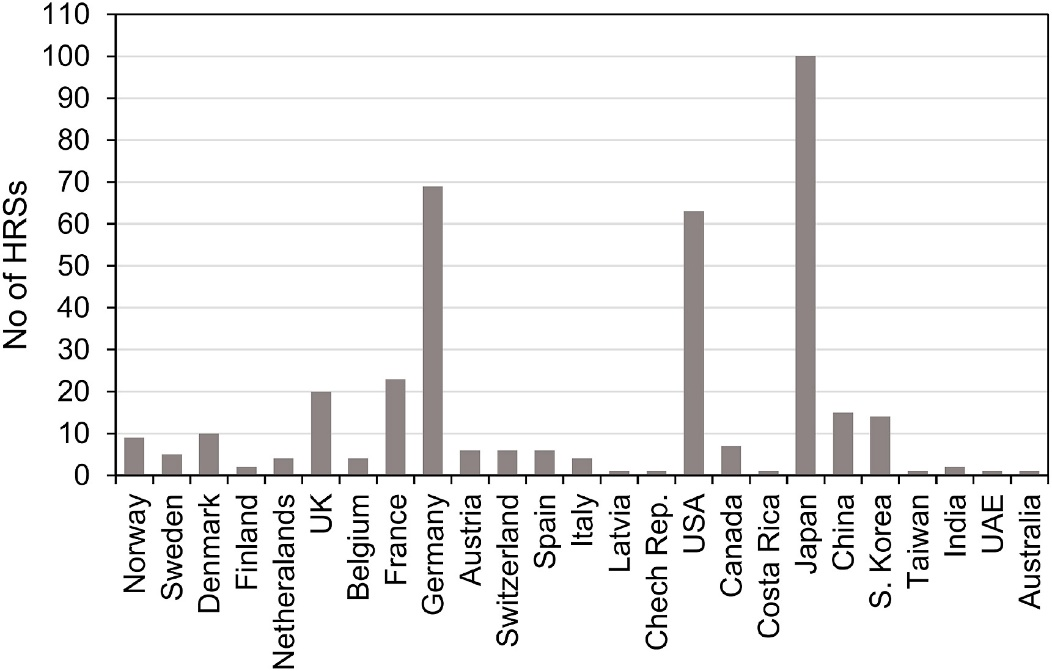
\includegraphics[width=0.6\linewidth]{image/hydrogen_refuel} \caption{Anzahl der Wasserstofftankstellen weltweit (Apostolou und Xydis, 2019)}\label{fig:unnamed-chunk-56}
\end{figure}

Im Europäischen Strategieplan für Energietechnologie werden Wasserstoff- und Brennstoffzellentechnologien als entscheidend für die Erreichung der Ziele zur Reduzierung der Treibhausgase bis 2050 vorgeschlagen (Roadmap Europe H., 2019; Alvarez-Meaza et al., 2020).

\hypertarget{relevante-initiativen-in-uxf6sterreich-61}{%
\subsection*{Relevante Initiativen in Österreich}\label{relevante-initiativen-in-uxf6sterreich-61}}
\addcontentsline{toc}{subsection}{Relevante Initiativen in Österreich}

\begin{itemize}
\tightlist
\item
  \href{https://fuelcellsworks.com/news/alstoms-hydrogen-train-successfully-completes-three-months-of-testing-in-austria/\#:~:text=Alstom's\%20Hydrogen\%20Train\%20Successfully\%20Completes\%20Three\%20Months\%20of\%20Testing\%20in\%20Austria,-By\%20FuelCellsWorksDecember\&text=Alstom's\%20Coradia\%20iLint\%2C\%20the\%20world's,Austrian\%20Federal\%20Railways}{hydrogen train}
\end{itemize}

\hypertarget{auswirkungen-in-bezug-auf-die-ziele-fuxfcr-nachhaltige-entwicklung-sdgs-61}{%
\subsection*{Auswirkungen in Bezug auf die Ziele für nachhaltige Entwicklung (SDGs)}\label{auswirkungen-in-bezug-auf-die-ziele-fuxfcr-nachhaltige-entwicklung-sdgs-61}}
\addcontentsline{toc}{subsection}{Auswirkungen in Bezug auf die Ziele für nachhaltige Entwicklung (SDGs)}

\begin{longtable}[]{@{}ccccc@{}}
\toprule
\begin{minipage}[b]{0.17\columnwidth}\centering
Ebene der Auswirkungen\strut
\end{minipage} & \begin{minipage}[b]{0.16\columnwidth}\centering
Indikator\strut
\end{minipage} & \begin{minipage}[b]{0.17\columnwidth}\centering
Richtung der Auswirkungen\strut
\end{minipage} & \begin{minipage}[b]{0.17\columnwidth}\centering
Beschreibung des Ziels \& SDG\strut
\end{minipage} & \begin{minipage}[b]{0.17\columnwidth}\centering
Quelle\strut
\end{minipage}\tabularnewline
\midrule
\endhead
\begin{minipage}[t]{0.17\columnwidth}\centering
Individuell\strut
\end{minipage} & \begin{minipage}[t]{0.16\columnwidth}\centering
Verbesserte Luftqualitaet\strut
\end{minipage} & \begin{minipage}[t]{0.17\columnwidth}\centering
\textbf{+}\strut
\end{minipage} & \begin{minipage}[t]{0.17\columnwidth}\centering
Gesundheit und Wohlbefinden (\emph{3})\strut
\end{minipage} & \begin{minipage}[t]{0.17\columnwidth}\centering
Colella, Jacobson \& Golden, 2005\strut
\end{minipage}\tabularnewline
\begin{minipage}[t]{0.17\columnwidth}\centering
Individuell\strut
\end{minipage} & \begin{minipage}[t]{0.16\columnwidth}\centering
Hohe Preise fuer Wasserstoffautos und Wasserstoffkraftstoff\strut
\end{minipage} & \begin{minipage}[t]{0.17\columnwidth}\centering
\textbf{-}\strut
\end{minipage} & \begin{minipage}[t]{0.17\columnwidth}\centering
Gleichheit (\emph{5,10})\strut
\end{minipage} & \begin{minipage}[t]{0.17\columnwidth}\centering
Kanna \& Paturu, 2020\strut
\end{minipage}\tabularnewline
\begin{minipage}[t]{0.17\columnwidth}\centering
Individuell\strut
\end{minipage} & \begin{minipage}[t]{0.16\columnwidth}\centering
Hoehere Anschaffungskosten aber niedrigere Betriebskosten fuer Privatpersonen\strut
\end{minipage} & \begin{minipage}[t]{0.17\columnwidth}\centering
\textbf{\textasciitilde{}}\strut
\end{minipage} & \begin{minipage}[t]{0.17\columnwidth}\centering
Nachhaltige wirtschaftliche Entwicklung (\emph{8,11})\strut
\end{minipage} & \begin{minipage}[t]{0.17\columnwidth}\centering
Apostolou \& Xydis, 2019\strut
\end{minipage}\tabularnewline
\begin{minipage}[t]{0.17\columnwidth}\centering
Systemisch\strut
\end{minipage} & \begin{minipage}[t]{0.16\columnwidth}\centering
Reduzierte Emissionen, verbesserte Luftqualitaet\strut
\end{minipage} & \begin{minipage}[t]{0.17\columnwidth}\centering
\textbf{+}\strut
\end{minipage} & \begin{minipage}[t]{0.17\columnwidth}\centering
Gesundheit und Wohlbefinden (\emph{3})\strut
\end{minipage} & \begin{minipage}[t]{0.17\columnwidth}\centering
Colella, Jacobson \& Golden, 2005\strut
\end{minipage}\tabularnewline
\begin{minipage}[t]{0.17\columnwidth}\centering
Systemisch\strut
\end{minipage} & \begin{minipage}[t]{0.16\columnwidth}\centering
Verteilung und Zuweisung von Guetern verschlechtert sich\strut
\end{minipage} & \begin{minipage}[t]{0.17\columnwidth}\centering
\textbf{-}\strut
\end{minipage} & \begin{minipage}[t]{0.17\columnwidth}\centering
Gleichheit (\emph{5,10})\strut
\end{minipage} & \begin{minipage}[t]{0.17\columnwidth}\centering
Kanna \& Paturu, 2020\strut
\end{minipage}\tabularnewline
\begin{minipage}[t]{0.17\columnwidth}\centering
Systemisch\strut
\end{minipage} & \begin{minipage}[t]{0.16\columnwidth}\centering
Geringere Emissionen, Ersatz von fossilen Brennstoffen, Energiewende\strut
\end{minipage} & \begin{minipage}[t]{0.17\columnwidth}\centering
\textbf{+}\strut
\end{minipage} & \begin{minipage}[t]{0.17\columnwidth}\centering
Oekologische Nachhaltigkeit (\emph{7,12-13,15})\strut
\end{minipage} & \begin{minipage}[t]{0.17\columnwidth}\centering
Colella, Jacobson \& Golden, 2005\strut
\end{minipage}\tabularnewline
\begin{minipage}[t]{0.17\columnwidth}\centering
Systemisch\strut
\end{minipage} & \begin{minipage}[t]{0.16\columnwidth}\centering
Noch nicht profitabel fuer Hersteller\strut
\end{minipage} & \begin{minipage}[t]{0.17\columnwidth}\centering
\textbf{-}\strut
\end{minipage} & \begin{minipage}[t]{0.17\columnwidth}\centering
Nachhaltige wirtschaftliche Entwicklung (\emph{8,11})\strut
\end{minipage} & \begin{minipage}[t]{0.17\columnwidth}\centering
Roadmap Europe, 2019\strut
\end{minipage}\tabularnewline
\begin{minipage}[t]{0.17\columnwidth}\centering
Systemisch\strut
\end{minipage} & \begin{minipage}[t]{0.16\columnwidth}\centering
Zahl der Wasserstofftankstellen steigt\strut
\end{minipage} & \begin{minipage}[t]{0.17\columnwidth}\centering
\textbf{+}\strut
\end{minipage} & \begin{minipage}[t]{0.17\columnwidth}\centering
Innovation und Infrastruktur (\emph{9})\strut
\end{minipage} & \begin{minipage}[t]{0.17\columnwidth}\centering
Apostolou \& Xydis, 2019\strut
\end{minipage}\tabularnewline
\begin{minipage}[t]{0.17\columnwidth}\centering
Systemisch\strut
\end{minipage} & \begin{minipage}[t]{0.16\columnwidth}\centering
Internationaler Austausch von Technologien\strut
\end{minipage} & \begin{minipage}[t]{0.17\columnwidth}\centering
\textbf{+}\strut
\end{minipage} & \begin{minipage}[t]{0.17\columnwidth}\centering
Partnerschaften und Kooperationen (\emph{17})\strut
\end{minipage} & \begin{minipage}[t]{0.17\columnwidth}\centering
International Partnership for Hydrogen and Fuel Cells in the Economy, n.d.\strut
\end{minipage}\tabularnewline
\bottomrule
\end{longtable}

\hypertarget{technologie--und-gesellschaftlicher-bereitschaftsgrad-57}{%
\subsection*{Technologie- und gesellschaftlicher Bereitschaftsgrad}\label{technologie--und-gesellschaftlicher-bereitschaftsgrad-57}}
\addcontentsline{toc}{subsection}{Technologie- und gesellschaftlicher Bereitschaftsgrad}

\begin{longtable}[]{@{}cc@{}}
\toprule
Stand der Technologiebereitschaft & Gesellschaftlicher Bereitschaftsgrad\tabularnewline
\midrule
\endhead
7-8 & 6-8\tabularnewline
\bottomrule
\end{longtable}

\hypertarget{offene-fragen-59}{%
\subsection*{Offene Fragen}\label{offene-fragen-59}}
\addcontentsline{toc}{subsection}{Offene Fragen}

\begin{enumerate}
\def\labelenumi{\arabic{enumi}.}
\tightlist
\item
  Wer wird den Fortschritt der Wasserstofftechnologie in der Schwerlastmobilität in Zukunft vorantreiben?
\item
  Wie lassen sich große Energiemengen bei geringem Gewicht und auf kleinem Raum im Fahrzeug speichern? (Roadmap Europa, 2019)
\end{enumerate}

\hypertarget{weitere-links-48}{%
\subsection*{Weitere links}\label{weitere-links-48}}
\addcontentsline{toc}{subsection}{Weitere links}

\begin{itemize}
\tightlist
\item
  \href{https://www.europarl.europa.eu/news/nl/press-room/20180911IPR13114/more-electric-cars-on-eu-roads-by-2030}{europarlament}
\item
  \href{https://ec.europa.eu/transport/themes/urban/vehicles/road/hydrogen_en}{ec.europa}
\item
  \href{https://www.fch.europa.eu/news/hydrogen-roadmap-europe-sustainable-pathway-european-energy-transition}{fch.europa}
\end{itemize}

\hypertarget{referenzen-61}{%
\subsection*{Referenzen}\label{referenzen-61}}
\addcontentsline{toc}{subsection}{Referenzen}

\begin{itemize}
\tightlist
\item
  Alvarez-Meaza, I., Zarrabeitia-Bilbao, E., Rio-Belver, R. M., \& Garechana-Anacabe, G. (2020). Fuel-Cell Electric Vehicles: Plotting a Scientific and Technological Knowledge Map. Sustainability, 12(6), 2334.
\item
  Apostolou, D., \& Xydis, G. (2019). A literature review on hydrogen refuelling stations and infrastructure. Current status and future prospects. Renewable and Sustainable Energy Reviews, 113(May), 109292. \url{https://doi.org/10.1016/j.rser.2019.109292}
\item
  Borgstedt, P., Neyer, B., \& Schewe, G. (2017). Paving the road to electric vehicles--A patent analysis of the automotive supply industry. Journal of cleaner production, 167, 75-87.
\item
  Colella, W. G., Jacobson, M. Z., \& Golden, D. M. (2005). Switching to a U.S. hydrogen fuel cell vehicle fleet: The resultant change in emissions, energy use, and greenhouse gases. Journal of Power Sources, 150, 150--181. \url{https://doi.org/https://doi.org/10.1016/j.jpowsour.2005.05.092}
\item
  Doppelbauer, M. (2020). Grundlagen der Elektromobilität. In Grundlagen der Elektromobilität. \url{https://doi.org/10.1007/978-3-658-29730-5}
\item
  Eichlseder, H., Klell, M., \& Trattner, A. (2018). Wasserstoff in der Fahrzeugtechnik. In Wasserstoff in der Fahrzeugtechnik. \url{https://doi.org/10.1007/978-3-8348-9674-2}
\item
  International Partnership for Hydrogen and Fuel Cells in the Economy. (n.d.). No Title. \url{https://www.iphe.net/}
\item
  Iribarren, D., Martín-Gamboa, M., Manzano, J., \& Dufour, J. (2016). Assessing the social acceptance of hydrogen for transportation in Spain: an unintentional focus on target population for a potential hydrogen economy. International journal of hydrogen energy, 41(10), 5203-5208.
\item
  Kanna, I. V., \& Paturu, P. (2020). A study of hydrogen as an alternative fuel. International Journal of Ambient Energy, 41(12), 1433--1436. \url{https://doi.org/10.1080/01430750.2018.1484803}
\item
  Lehmann, J., \& Luschtinetz, T. (2014). Wasserstoff und Brennstoffzellen.
\item
  Roadmap Europe (2019). A sustainable pathway for the European energy transition. Luxembourg: Publications Office of the European Union.
\item
  Pötscher, F., Winter, R., Lichtblau, G., Schreiber, H., \& Kutschera, U. (2014). Ökobilanz alternativer Antriebe -- Elektrofahrzeuge im Vergleich.
\item
  Schabbach, T., \& Wesselak, V. (2020). Energie - Den Erneuerbaren gehört die Zukunft.
\item
  Tanç, B., Arat, H. T., Baltacıoğlu, E., \& Kadir, A. (2019). Overview of the next quarter century vision of hydrogen fuel cell electric vehicles. In International Journal of Hydrogen Energy, Volume 44, Issue 20, (pp.~10120--10128).
\item
  Töpler, J., \& Lehmann, J. (2017). Wasserstoff und Brennstoffzelle - Technologien und Marktkonzepte. In Springer Vieweg.
\end{itemize}

\hypertarget{bev}{%
\section{Batterieelektrisch}\label{bev}}

\hypertarget{synonyme-54}{%
\subsection*{Synonyme}\label{synonyme-54}}
\addcontentsline{toc}{subsection}{Synonyme}

\emph{Batteriebetriebenes Elektrofahrzeug (BEV- battery electric vehicle)}

\hypertarget{definition-62}{%
\subsection*{Definition}\label{definition-62}}
\addcontentsline{toc}{subsection}{Definition}

Der Verkehr trägt mit bis zu 30\% zu den klimarelevanten Treibhausgasemissionen in Österreich bei, wobei CO\textsubscript{2} die größte Rolle spielt (Bundesministerium für Umwelt, 2019). Während die durchschnittliche Motorleistung der jährlich verkauften Fahrzeuge steigt (Kreuzer, 2020), steigen auch die Gesamtemissionen des Verkehrssektors (Bundesministerium für Umwelt, 2019). Ohne eine Änderung des Mobilitätsverhaltens kann nur ein Umstieg auf lokal emissionsfreie Antriebstechnologien, wie BEVs, Abhilfe schaffen. BEVs sind im Betrieb emissionsfrei (abgesehen von Reifenverschleiß und minimalem Bremsstaub) und haben einen Batteriespeicher/Akkumulator eingebaut, der an einer externen Ladestation aufgeladen wird. Die Energieumwandlung erfolgt in einem Elektromotor. Die Vor- und Nachteile von BEVs sind in der folgenden Tabelle dargestellt.

\begin{longtable}[]{@{}cc@{}}
\toprule
\begin{minipage}[b]{0.47\columnwidth}\centering
Vorteile\strut
\end{minipage} & \begin{minipage}[b]{0.47\columnwidth}\centering
Nachteile\strut
\end{minipage}\tabularnewline
\midrule
\endhead
\begin{minipage}[t]{0.47\columnwidth}\centering
\textbf{Weniger Laerm}: Elektromotoren arbeiten wesentlich leiser als Verbrennungsmotoren. Im Autoverkehr wird der meiste Laerm jedoch nicht vom Motor erzeugt, sondern durch das Zusammenspiel von Reifen und Fahrbahn oder - bei hohen Geschwindigkeiten - durch aerodynamische Geraeusche. In diesen Faellen gibt es keinen Unterschied zwischen einem Elektroauto und einem herkoemmlichen Fahrzeug. Schon ab etwa 25 Stundenkilometern sind die Abrollgeraeusche beim Autofahren entscheidend. Unterhalb dieser Geschwindigkeit ist das Motorgeraeusch die entscheidende Geraeuschquelle. Daher sind Elektroautos in Gebieten mit niedriger Geschwindigkeit, wie etwa in Wohngebieten oder beim Anfahren an Kreuzungen und Ampeln, leiser.\strut
\end{minipage} & \begin{minipage}[t]{0.47\columnwidth}\centering
Die \textbf{Reichweite} variiert derzeit von ca. 120 bis \textasciitilde{} 600 km. Das Tesla Model S kann nach Angaben des Herstellers bis zu 610 km weit fahren und hat damit die groesstmoegliche Reichweite unter den E-Autos, das Auto kostet knapp 80.000 Euro. Die Reichweite haengt von vielen Faktoren ab, wie z.B. von der unterschiedlichen Fahrweise, den Witterungsbedingungen (er erreicht seine volle Kapazitaet nur in einem Temperaturbereich zwischen 20 und 40 Grad Celsius), der Nutzung der Klimaanlage. Dennoch sind 94\% aller Autofahrten der oesterreichischen Bevoelkerung kuerzer als 50 km.\strut
\end{minipage}\tabularnewline
\begin{minipage}[t]{0.47\columnwidth}\centering
\textbf{Lokal emissionsfrei}: BEVs emittieren keine Luftschadstoffe, wenn sie in Betrieb sind. Die Reduktion von Treibhausgasen ist stark abhaengig von den Energietraegern, mit denen der Strom zuvor erzeugt wurde und den daraus resultierenden Emissionen. Der oesterreichische Strommix hat bereits einen hohen Anteil an erneuerbarer Energie. Der zusaaetzliche Strombedarf, der durch die Elektromobilitaet entsteht, wird durch die Ausbauplaene bis 2020 fuer die Stromerzeugung aus erneuerbaren Energietraegern um ein Vielfaches gedeckt. Dies stellt eine hervorragende Situation fuer die Elektromobilitaet in Oesterreich dar.\strut
\end{minipage} & \begin{minipage}[t]{0.47\columnwidth}\centering
\textbf{Elektrizitaetsbedarf}: Mit zunehmender Anzahl von Elektrofahrzeugen auf Oesterreichs Strassen kann es zu unterschiedlichen Belastungen des Niederspannungsnetzes kommen, was zu Spannungsschwankungen und Unterbrechungen fuehren kann. Wenn daher mittel- bis langfristig ein gesteuertes Laden notwendig ist, sollte dies bei der Planung und Errichtung von Ladepunkten beruecksichtigt werden. Es muss jedoch darauf geachtet werden, dass die Steuerung den Kundeninteressen entspricht.\strut
\end{minipage}\tabularnewline
\begin{minipage}[t]{0.47\columnwidth}\centering
\textbf{Anschaffungskosten}: Die guenstigsten Elektroautos sind bereits ab 16.000 Euro erhaeltlich.\strut
\end{minipage} & \begin{minipage}[t]{0.47\columnwidth}\centering
Das \textbf{System des Schnellladens} ist kostenintensiv sowie sicherheitstechnisch anspruchsvoll und stellt aufgrund des hohen Leistungsbedarfs (\textgreater{} 20 kW pro Anschluss) besondere Anforderungen an das Stromnetz. Solche Ladestationen sollten vor allem dort installiert werden, wo sie mit dem Netz kompatibel und wirtschaftlich sind. Daher ist vor der Installation von Schnellladestationen eine Kosten-Nutzen-Bewertung ratsam.\strut
\end{minipage}\tabularnewline
\begin{minipage}[t]{0.47\columnwidth}\centering
\textbf{Kosten fuer das Aufladen}: Wird das Elektroauto mit Haushaltsstrom geladen, liegen die Kosten bei knapp 28 Cent/kWh, an oeffentlichen Ladestationen schwanken sie zwischen 30-60 Cent. Fuer 100 km im E-Auto kostet der Strom zum Laden etwa 4,50. Die entsprechenden Kosten fuer Benzin und Diesel im Vergleich: bei einem Verbrauch von 6 Litern Benzin bzw. 5 Litern Diesel derzeit 8,40 Euro und 6,70 Euro (Michael, 2020).\strut
\end{minipage} & \begin{minipage}[t]{0.47\columnwidth}\centering
Die \textbf{Ladedauer} haengt von der Batteriekapazitaet und der Ladeleistung ab. An oeffentlichen Schnellladestationen betraegt die Dauer etwa eine halbe Stunde bis eine Stunde. An einer Haushaltssteckdose 8-14 Stunden.\strut
\end{minipage}\tabularnewline
\begin{minipage}[t]{0.47\columnwidth}\centering
\textbf{Ladestationen}: Die Zahl der Ladestationen und Ladepunkte nimmt in Oesterreich stetig zu und liegt derzeit bei 5.000 oeffentlich zugaenglichen Ladepunkten. Zum Vergleich: In Oesterreich gibt es knapp 2800 Tankstellen (Sitte, 2019).\strut
\end{minipage} & \begin{minipage}[t]{0.47\columnwidth}\centering
-\strut
\end{minipage}\tabularnewline
\bottomrule
\end{longtable}

\hypertarget{wichtige-interessensgruppen-62}{%
\subsection*{Wichtige Interessensgruppen}\label{wichtige-interessensgruppen-62}}
\addcontentsline{toc}{subsection}{Wichtige Interessensgruppen}

\begin{itemize}
\tightlist
\item
  \textbf{Betroffene}: Fahrer:innen konventioneller Autos, Autohersteller, Versicherungen
\item
  \textbf{Verantwortliche}: Nationale Regierungen, Stadtverwaltungen, Privatunternehmen, internationale Lobbyisten
\end{itemize}

\hypertarget{aktueller-stand-der-wissenschaft-und-forschung-62}{%
\subsection*{Aktueller Stand der Wissenschaft und Forschung}\label{aktueller-stand-der-wissenschaft-und-forschung-62}}
\addcontentsline{toc}{subsection}{Aktueller Stand der Wissenschaft und Forschung}

Die Forschung zu diesem Thema konzentriert sich hauptsächlich auf die Leistung der Technologie, die Dimensionierung der Komponenten, die Ladestationen und die Ökobilanz (LCA). Die Ökobilanz ist ein Instrument zur Bewertung des ökologischen Fußabdrucks eines Produkts, eines Prozesses oder einer Tätigkeit während seines/ihres gesamten Lebenszyklus (Roy et al., 2009). Die wichtigsten Faktoren, die die Ökobilanz von BEVs beeinflussen, sind die Herstellung des Fahrzeugs und die Bereitstellung von Strom für seinen Betrieb. Während des Betriebs fallen keine direkten Emissionen an, aber die Quelle der Stromversorgung beeinflusst die Menge der indirekten Emissionen. Alte Batterien können als stationäre Stromspeicher wiederverwendet werden. Durch das Recycling der Batterien können diese wieder als Rohstoffquelle genutzt werden. Für die Herstellung von batterieelektrischen Antrieben werden folgende Rohstoffe benötigt: Lithium für die Lithium-Ionen-Batterie, Kobalt ebenfalls für die Batterie, wobei der Bedarf rückläufig ist, und Kupfer als Leitermaterial. Außerdem werden Seltene Erden benötigt, insbesondere Neodym und Dysprosium für Permanentmagnete; diese werden nicht mehr benötigt, wenn sie durch eine andere Motortechnologie ersetzt werden (Doppelbauer, 2020).

In der nachstehenden Tabelle werden die CO2-Emissionen (in Tonnen) bei der Herstellung von Fahrzeugen mit Verbrennungsmotor (ICE - internal combustion engine) und batteriebetriebenen Fahrzeugen verglichen, wobei die Größe des Fahrzeugs berücksichtigt wird. Es wird deutlich, dass BEV während des Produktionsprozesses zwischen 3 und 9 Tonnen CO2 mehr erzeugen als ICE (Doppelbauer, 2020).

\begin{longtable}[]{@{}ccccccc@{}}
\toprule
& & ICE & & & BEV &\tabularnewline
\midrule
\endhead
& Klein & Mittel & Gross & Klein (30 kWh) & Mittel (60 kWh) & Gross (90 kWh)\tabularnewline
Karosserie des Fahrzeugs & 2.5 & 3.8 & 5.0 & 2.5 & 3.8 & 5.0\tabularnewline
Zusaetzliche Komponenten & 0.5 & 0.65 & 0.8 & 0.5 & 0.65 & 0.8\tabularnewline
HV-System & - & - & - & 0.3 & 0.55 & 0.7\tabularnewline
Antrieb & 0.4 & 0.6 & 0.8 & 0.2 & 0.25 & 0.3\tabularnewline
Produktion & 1.5 & 1.5 & 1.5 & 1.5 & 1.5 & 1.5\tabularnewline
Batterie & - & - & - & 3 & 6 & 9\tabularnewline
\textbf{Gesamt} & \textbf{4.9} & \textbf{6.6} & \textbf{8.1} & \textbf{8} & \textbf{12.8} & \textbf{17.3}\tabularnewline
\bottomrule
\end{longtable}

In dieser Ökobilanz werden auch aktuelle Daten zur Produktion von Batteriesystemen für Elektrofahrzeuge berücksichtigt. Zwar ist die Herstellung von Batterien mit einem erheblichen Energieaufwand und damit mit hohen Emissionen verbunden, jedoch entfallen bei Elektrofahrzeugen Komponenten wie Getriebe und Abgasnachbehandlung und deren produktionsbedingte Emissionen.

Entscheidend für die Treibhausgasbilanz von Fahrzeugen ist vor allem die Energie, die für den Betrieb des Fahrzeugs eingesetzt wird. Während der Einsatz fossiler Energie bei Benzin- und Dieselfahrzeugen zu hohen Treibhausgasemissionen führt, haben Elektrofahrzeuge keine direkten Treibhausgasemissionen in ihrer Bilanz. Unter Berücksichtigung der direkten und indirekten Emissionen kann die Nutzung eines Elektroautos, das mit Strom aus erneuerbaren Quellen betrieben wird, 80 \% der Treibhausgasemissionen im Vergleich zu einem mit fossilen Brennstoffen betriebenen Fahrzeug einsparen. Darüber hinaus werden durch die Nutzung von Strom aus erneuerbaren Energien auch die Stickoxidemissionen erheblich reduziert. Die Partikelemissionen hingegen steigen je nach Stromquelle leicht an.

Die Vorteile des Elektroantriebs zeigen sich auch im kumulierten Energieverbrauch, abhängig von der Qualität des Stroms. Hervorzuheben ist der geringere spezifische Verbrauch im Vergleich zu fossil befeuerten Fahrzeugen. Dies ist auf den hohen Wirkungsgrad des Elektromotors zurückzuführen (Fritz et al., 2018). Die negativen ökologischen und sozialen Auswirkungen der Gewinnung der seltenen Rohstoffe, die zur Herstellung der Batterie benötigt werden, werden bereits reduziert. Die Bundesregierung fördert die Forschung zur wirtschaftlichen Nutzung und Rückgewinnung von Rohstoffen und zur Wiederverwendung von Batterien (Second Life). Inzwischen gibt es auch Batterien, die deutlich weniger Kobalt benötigen. Auch die Industrie engagiert sich zunehmend in Initiativen zur nachhaltigen Versorgung mit dem Rohstoff (Responsible Mining) (Kurzempa, 2018).
Was die Effizienz dieser Technologie betrifft, so liegt der Well-to-Wheel-Wirkungsgrad in Österreich bei etwa 69\%. Dies ist ein erheblicher Effizienzgewinn im Vergleich zu einem Brennstoffzellenauto mit einem durchschnittlichen Well-to-Wheel-Wirkungsgrad von etwa 27 \% und einem benzinbetriebenen Auto mit etwa 20 \% (Bundesministerium für Umwelt Naturschutz und nukleare Sicherheit, n.d.). Die Verluste im Stromnetz in Österreich sind sehr gering und können im Bereich von 5 \% angesetzt werden, woraus sich bei 100 \% Ökostrom ein Quelle-Tank-Wirkungsgrad (well-to-tank) von 95 \% ergibt. Im Zuge des Ladevorgangs entstehen durch Widerstände im Ladekabel und in der Batterie Ladeverluste von 10\%. Der Traktionsbatterie ist jedoch ein AC/DC-Spannungswandler (Gleichrichter) vorgeschaltet, der weitere 5\% Energieverluste verursacht. Um die gespeicherte Energie auf die Straße zu bringen, fließt sie nun durch einen Gleich-/Wechselspannungswandler (Inverter) mit 5\% Energieverlust und kann schließlich von einem Elektromotor mit 90\% Wirkungsgrad auf das Rad übertragen werden. Der Tank-zu-Rad-Wirkungsgrad (tank-to-wheel) beträgt somit 73 \%. Der Gesamtwirkungsgrad eines BEV vom Tank zum Rad liegt bei 69 \%.

\hypertarget{aktueller-stand-der-praktischen-umsetzung-62}{%
\subsection*{Aktueller Stand der praktischen Umsetzung}\label{aktueller-stand-der-praktischen-umsetzung-62}}
\addcontentsline{toc}{subsection}{Aktueller Stand der praktischen Umsetzung}

Die Zahl der weltweit zugelassenen E-Autos hat einen neuen Rekordstand erreicht. Gleichzeitig hat sich aber das Wachstum der Neuzulassungen abgeschwächt. Im Jahr 2019 waren weltweit rund 7,9 Millionen E-Autos zugelassen. Die Zahl der Neuzulassungen hingegen hatte im Jahr 2018 noch ein plus von 74\% gegenüber dem Jahr 2017 (1,3 Millionen zu 2,2 Millionen), im Jahr 2019 blieben die Neuzulassungen jedoch fast auf der gleichen Höhe wie im Jahr 2018 mit einem plus von 4\% (2,3 Millionen im Jahr 2019) (Prack, 2020).
Laut dem Zentrum für Sonnenenergie- und Wasserstoff-Forschung Baden-Württemberg (ZSW) ist diese Entwicklung vor allem auf die Kürzung der E-Auto-Förderung in China und den USA zurückzuführen. Dennoch wurde in diesen Ländern fast das Neuzulassungsniveau des Vorjahres erreicht: In China wurden 1.204.000 Neuzulassungen registriert (52.000 weniger), in den USA 329.500 (31.800 weniger). Deutschland liegt mit rund 230.000 zugelassenen Fahrzeugen an siebter Stelle bei der Gesamtzahl der E-Autos nach China, den USA, Norwegen, Japan, Frankreich und Großbritannien (Prack, 2020).
Doch nicht nur für den Individualverkehr ist der Elektroantrieb eine Alternative. Auch im gewerblichen und öffentlichen Verkehr werden immer mehr Fahrzeuge elektrisch angetrieben. Je größer und schwerer ein Fahrzeug ist, desto schwieriger ist es, es aufgrund der enormen Masse der großen Batterien zu elektrifizieren. Die Batterietechnologie entwickelt sich jedoch ständig weiter, und die Reichweiten werden immer größer. Selbst schwere Sattelschlepper könnten in naher Zukunft elektrifiziert werden. Sie bräuchten allerdings Batterien und Oberleitungen auf den Autobahnen, damit sie auf ihren Strecken schnell aufgeladen werden können. Das wird jetzt in Deutschland getestet. Drei Strecken in Hessen, Schleswig-Holstein und Baden-Württemberg werden derzeit mit Oberleitungen ausgestattet (mehr dazu im Abschnitt über \protect\hyperlink{ers}{Electric Road Systems}). In vielen Städten, wie Köln, Berlin und Hamburg, gehören Elektrobusse bereits zum Linienverkehr. Ihr Strombedarf wird durch schnelles, gelegentliches Aufladen an Haltestellen und durch nächtliches Aufladen in Betriebshöfen gedeckt. Viele deutsche Städte planen, in naher Zukunft vollelektrische Busse einzusetzen (Kurzempa, 2018).

\hypertarget{relevante-initiativen-in-uxf6sterreich-62}{%
\subsection*{Relevante Initiativen in Österreich}\label{relevante-initiativen-in-uxf6sterreich-62}}
\addcontentsline{toc}{subsection}{Relevante Initiativen in Österreich}

\begin{itemize}
\tightlist
\item
  \href{https://www.oeamtc.at/thema/elektromobilitaet/alles-ueber-elektroautos-35420295}{oeamtc.at}
\item
  \href{https://www.beoe.at/statistik/}{beoe.at}
\end{itemize}

\hypertarget{auswirkungen-in-bezug-auf-die-ziele-fuxfcr-nachhaltige-entwicklung-sdgs-62}{%
\subsection*{Auswirkungen in Bezug auf die Ziele für nachhaltige Entwicklung (SDGs)}\label{auswirkungen-in-bezug-auf-die-ziele-fuxfcr-nachhaltige-entwicklung-sdgs-62}}
\addcontentsline{toc}{subsection}{Auswirkungen in Bezug auf die Ziele für nachhaltige Entwicklung (SDGs)}

\begin{longtable}[]{@{}ccccc@{}}
\toprule
\begin{minipage}[b]{0.17\columnwidth}\centering
Ebene der Auswirkungen\strut
\end{minipage} & \begin{minipage}[b]{0.16\columnwidth}\centering
Indikator\strut
\end{minipage} & \begin{minipage}[b]{0.17\columnwidth}\centering
Richtung der Auswirkungen\strut
\end{minipage} & \begin{minipage}[b]{0.17\columnwidth}\centering
Beschreibung des Ziels \& SDG\strut
\end{minipage} & \begin{minipage}[b]{0.17\columnwidth}\centering
Quelle\strut
\end{minipage}\tabularnewline
\midrule
\endhead
\begin{minipage}[t]{0.17\columnwidth}\centering
Individuell\strut
\end{minipage} & \begin{minipage}[t]{0.16\columnwidth}\centering
Weniger Laerm\strut
\end{minipage} & \begin{minipage}[t]{0.17\columnwidth}\centering
\textbf{+}\strut
\end{minipage} & \begin{minipage}[t]{0.17\columnwidth}\centering
Gesundheit und Wohlbefinden (\emph{3})\strut
\end{minipage} & \begin{minipage}[t]{0.17\columnwidth}\centering
Bundesministerium fuer Umwelt, 2019\strut
\end{minipage}\tabularnewline
\begin{minipage}[t]{0.17\columnwidth}\centering
Individuell\strut
\end{minipage} & \begin{minipage}[t]{0.16\columnwidth}\centering
Lokal emissionsfrei\strut
\end{minipage} & \begin{minipage}[t]{0.17\columnwidth}\centering
\textbf{+}\strut
\end{minipage} & \begin{minipage}[t]{0.17\columnwidth}\centering
Oekologische Nachhaltigkeit (\emph{7,12,13,15})\strut
\end{minipage} & \begin{minipage}[t]{0.17\columnwidth}\centering
Bundesministerium fuer Umwelt, 2019\strut
\end{minipage}\tabularnewline
\begin{minipage}[t]{0.17\columnwidth}\centering
Individuell\strut
\end{minipage} & \begin{minipage}[t]{0.16\columnwidth}\centering
Geringere Reisekosten\strut
\end{minipage} & \begin{minipage}[t]{0.17\columnwidth}\centering
\textbf{+}\strut
\end{minipage} & \begin{minipage}[t]{0.17\columnwidth}\centering
Nachhaltige wirtschaftliche Entwicklung (\emph{8,11})\strut
\end{minipage} & \begin{minipage}[t]{0.17\columnwidth}\centering
Michael, 2020\strut
\end{minipage}\tabularnewline
\begin{minipage}[t]{0.17\columnwidth}\centering
Systemisch\strut
\end{minipage} & \begin{minipage}[t]{0.16\columnwidth}\centering
Emissionsfrei, aber hohe Emissionen in der Produktion\strut
\end{minipage} & \begin{minipage}[t]{0.17\columnwidth}\centering
\textbf{\textasciitilde{}}\strut
\end{minipage} & \begin{minipage}[t]{0.17\columnwidth}\centering
Oekologische Nachhaltigkeit (\emph{7,12,13,15})\strut
\end{minipage} & \begin{minipage}[t]{0.17\columnwidth}\centering
Fritz et al., 2018\strut
\end{minipage}\tabularnewline
\begin{minipage}[t]{0.17\columnwidth}\centering
Systemisch\strut
\end{minipage} & \begin{minipage}[t]{0.16\columnwidth}\centering
Zunehmende Anzahl von Ladestationen und Weiterentwicklung der Batterietechnologie\strut
\end{minipage} & \begin{minipage}[t]{0.17\columnwidth}\centering
\textbf{+}\strut
\end{minipage} & \begin{minipage}[t]{0.17\columnwidth}\centering
Innovation und Infrastruktur (\emph{9})\strut
\end{minipage} & \begin{minipage}[t]{0.17\columnwidth}\centering
Sitte, 2019; Kurzempa, 2018\strut
\end{minipage}\tabularnewline
\begin{minipage}[t]{0.17\columnwidth}\centering
Systemisch\strut
\end{minipage} & \begin{minipage}[t]{0.16\columnwidth}\centering
Initiative fuer Elektrofahrzeuge zur Beschleunigung der Einfuehrung und Uebernahme von Elektrofahrzeugen weltweit\strut
\end{minipage} & \begin{minipage}[t]{0.17\columnwidth}\centering
\textbf{+}\strut
\end{minipage} & \begin{minipage}[t]{0.17\columnwidth}\centering
Partnerschaften und Kooperationen (\emph{17})\strut
\end{minipage} & \begin{minipage}[t]{0.17\columnwidth}\centering
IEA, 2020\strut
\end{minipage}\tabularnewline
\bottomrule
\end{longtable}

\hypertarget{technologie--und-gesellschaftlicher-bereitschaftsgrad-58}{%
\subsection*{Technologie- und gesellschaftlicher Bereitschaftsgrad}\label{technologie--und-gesellschaftlicher-bereitschaftsgrad-58}}
\addcontentsline{toc}{subsection}{Technologie- und gesellschaftlicher Bereitschaftsgrad}

\begin{longtable}[]{@{}cc@{}}
\toprule
Stand der Technologiebereitschaft & Gesellschaftlicher Bereitschaftsgrad\tabularnewline
\midrule
\endhead
8-9 & 7-9\tabularnewline
\bottomrule
\end{longtable}

\hypertarget{offene-fragen-60}{%
\subsection*{Offene Fragen}\label{offene-fragen-60}}
\addcontentsline{toc}{subsection}{Offene Fragen}

\begin{enumerate}
\def\labelenumi{\arabic{enumi}.}
\tightlist
\item
  Wie können Versorgungsengpässe entlang der Wertschöpfungskette behoben werden?
\item
  Wie groß ist die potenzielle Verlagerung der Abhängigkeit von ölproduzierenden auf lithiumproduzierende Länder? Was ist der erwartete Zeitrahmen?
\item
  Welche Rolle spielt die Sekundärnutzung von Fahrzeugbatterien?
\item
  Wie können lokale Regierungen das Bewusstsein der Verbraucher:innen für BEVs stärken?
\end{enumerate}

\hypertarget{weitere-links-49}{%
\subsection*{Weitere links}\label{weitere-links-49}}
\addcontentsline{toc}{subsection}{Weitere links}

\begin{itemize}
\tightlist
\item
  \href{https://www.bmu.de/fileadmin/Daten_BMU/Pools/Broschueren/elektromobilitaet_broschuere_en_bf.pdf}{bmu.de}
\item
  \href{https://publik.tuwien.ac.at/files/publik_272020.pdf}{publik.tuwien.ac.at}
\item
  \href{https://www.isi.fraunhofer.de/content/dam/isi/dokumente/cct/2020/Fact_check_Batteries_for_electric_cars.pdf}{isi.fraunhofer.de}
\item
  \href{https://www.kleinezeitung.at/auto/elektroauto/5479610/Jaenner-bis-Dezember-2020_Das-sind-die-meistverkauften\#image-01_Volkswagen-e-Golf-2017-1600-01_1534157268197687_v0_h}{kleinezeitung.at}
\item
  \href{https://www.volkswagen.at/elektroauto/id-magazin/mobilitaet/elektromobilitaet-europa}{volkswagen.at}
\item
  \href{https://www.adac.de/rund-ums-fahrzeug/elektromobilitaet/kaufen/elektroautos-uebersicht/}{adac.de}
\item
  \href{https://ec.europa.eu/eurostat/databrowser/view/ROAD_EQR_CARPDA__custom_91702/bookmark/table?lang=de\&bookmarkId=7e47ef9d-b80b-4bd6-a35b-046cb5af4500}{ec.europa.eu}
\end{itemize}

\hypertarget{referenzen-62}{%
\subsection*{Referenzen}\label{referenzen-62}}
\addcontentsline{toc}{subsection}{Referenzen}

\begin{itemize}
\tightlist
\item
  Bundesministerium für Umwelt, N. und nukleare S. (BMU). (2019). Wie umweltfreundlich sind Elektroautos? 1--20. www.bmu.de
\item
  Bundesministerium für Umwelt Naturschutz und nukleare Sicherheit. (n.d.). Effizienz und Kosten: Lohnt sich der Betrieb eines Elektroautos? \textbar{} BMU. Available at: \url{https://www.bmu.de/themen/luft-laerm-verkehr/verkehr/elektromobilitaet/effizienz-und-kosten/} {[}Accessed: 19 February 2021{]}
\item
  Doppelbauer, M. (2020). Grundlagen der Elektromobilität. In Grundlagen der Elektromobilität. \url{https://doi.org/10.1007/978-3-658-29730-5}
\item
  Eichlseder, H., Klell, M., \& Trattner, A. (2018). Wasserstoff in der Fahrzeugtechnik. In Wasserstoff in der Fahrzeugtechnik. \url{https://doi.org/10.1007/978-3-8348-9674-2}
\item
  Fritz, D., Heinfellner, H., Lichtblau, G., Pölz, W., \& Stranner, G. (2018). Update: Ökobilanz alternativer Antriebe. 1--16. \url{https://umweltbundesamt.at/fileadmin/site/publikationen/DP152.pdf}
\item
  IEA. (2020, October 26). Electric Vehicles Initiative -- Programmes and partnerships - IEA. \url{https://www.iea.org/areas-of-work/programmes-and-partnerships/electric-vehicles-initiative}
\item
  Kreuzer, C. (2020, September 8). Österreicher fahren auf immer PS-stärkere Autos ab \textbar{} Wiener Städtische. \url{https://www.wienerstaedtische.at/unternehmen/presse/pressemeldungen/detail/oesterreicher-fahren-auf-immer-ps-staerkere-autos-ab.html}
\item
  Kurzempa, A. (2018). Electromobility -- what does it mean? AUTOBUSY -- Technika, Eksploatacja, Systemy Transportowe, 19(6), 894--897. \url{https://doi.org/10.24136/atest.2018.197}
\item
  Lehmann, J., \& Luschtinetz, T. (2014). Wasserstoff und Brennstoffzellen.
\item
  Michael. (2020, January 26). Wasserstoff, E-Auto, E-Fuels: Warum das E-Auto die beste Alternative ist \textbar{} Elektroauto-News.net. \url{https://www.elektroauto-news.net/2020/wasserstoff-e-auto-e-fuels-batterieauto-beste-alternative}
\item
  Pötscher, F., Winter, R., Lichtblau, G., Schreiber, H., \& Kutschera, U. (2014). Ökobilanz alternativer Antriebe -- Elektrofahrzeuge im Vergleich.
\item
  Prack, N. (2020, February 27). Anzahl der Elektroautos: Deutschland \& Ausland \textbar{} ADAC. \url{https://www.adac.de/news/statistik-e-autos/}
\item
  Roy, P., Nei, D., Orikasa, T., Xu, Q., Okadome, H., Nakamura, N., \& Shiina, T. (2009). A review of life cycle assessment (LCA) on some food products. Journal of Food Engineering, 90(1), 1--10. \url{https://doi.org/https://doi.org/10.1016/j.jfoodeng.2008.06.016}
\item
  Schabbach, T., \& Wesselak, V. (2020). Energie - Den Erneuerbaren gehört die Zukunft.
\item
  Sitte, P. (2019, January 21). E-Mobilität: Zahl der Ladestationen für Elektroautos steigt weiter an \textbar{} Bundesverband Elektromobilität Österreich (BEÖ), 21.01.2019. \url{https://www.ots.at/presseaussendung/OTS_20190121_OTS0048/e-mobilitaet-zahl-der-ladestationen-fuer-elektroautos-steigt-weiter-an-bild}
\item
  Töpler, J., \& Lehmann, J. (2017). Wasserstoff und Brennstoffzelle - Technologien und Marktkonzepte. In Springer Vieweg.
\end{itemize}

\hypertarget{plugin_hybrid}{%
\section{Plugin-Hybridfahrzeuge}\label{plugin_hybrid}}

\hypertarget{synonyme-55}{%
\subsection*{Synonyme}\label{synonyme-55}}
\addcontentsline{toc}{subsection}{Synonyme}

\emph{Hybrid, Hybrid-Elektrofahrzeuge (HEV - hybrid eletric vehicles), Plug-in-Hybrid-Elektrofahrzeuge (PHEV - Plug-in hybrid electric vehicles)}

\hypertarget{definition-63}{%
\subsection*{Definition}\label{definition-63}}
\addcontentsline{toc}{subsection}{Definition}

Plug-in-Hybridfahrzeuge kombinieren den Elektroantrieb entweder mit einem herkömmlichen Verbrennungsmotor oder mit anderen Motoren, die alternative Kraftstoffe verwenden. Das hat den Vorteil, dass die Fahrzeuge lange Strecken zurücklegen können, aber Verbrauch und Emissionen sinken. Ein Energiemanagementsystem sorgt dafür, dass während der Fahrt die optimale Menge an Energie aus den beiden Energiequellen bezogen wird. Das Verhältnis des Energieverbrauchs wird durch den Fahrzyklus beeinflusst. Je schneller das Fahrzeug fährt, desto mehr Energie wird benötigt (Aswin und Senthilmurugan, 2018).

Die Vorteile eines Hybridfahrzeugs liegen in der geringeren CO2-Bilanz, der höheren Kilometerleistung im Vergleich zu herkömmlichen Fahrzeugen, der finanziellen Unterstützung beim Kauf, den niedrigeren jährlichen Kosten und dem regenerativen Bremssystem. Zu den Nachteilen gehören hohe Anschaffungskosten, eine geringere Kraftstoffeffizienz, da die zusätzlich eingebauten Teile mehr Platz beanspruchen und zusätzliches Gewicht verursachen, sowie höhere Wartungskosten aufgrund des Doppelmotors. Außerdem wurden Bedenken geäußert, dass die Batterie im Falle eines Unfalls explodieren könnte (Aswin und Senthilmurugan, 2018).

Der oben erwähnte Sicherheitsaspekt kann jedoch vernachlässigt werden, da die Ergebnisse des EuroNCAP-Crashtests zeigen, dass Hybridfahrzeuge genauso sicher sind wie Fahrzeuge mit konventionellem Antriebssystem. Als Beispiel dient auch die Hybrid-Synergy-Drive-Technologie (HSD) von Toyota, bei der das Hybridsystem - basierend auf dem Airbag-Auslösesignal - im Falle eines Unfalls sofort alle elektrischen Systeme abschaltet und den Batteriekontakt unterbricht (ADAC, 2019).

Derzeit gibt es mehrere Arten von Hybridfahrzeugen auf dem Markt:

\begin{itemize}
\tightlist
\item
  Serieller Hybrid
\end{itemize}

Das serielle Hybridmodell besteht aus einem Verbrennungsmotor, der einen Generator antreibt, anstatt die Räder direkt anzutreiben. Die Räder des Fahrzeugs erhalten ihre Kraft von den Elektromotoren. Der Generator treibt sowohl die Ladebatterie als auch die Räder des Fahrzeugs an. Serienhybride erzeugen die maximale Energie bei der Beschleunigung und geben die Energie beim regenerativen Bremsen zurück. Die Elektrofahrzeuge sind so konzipiert, dass an jedes Rad ein Motor angeschlossen ist. Die Kombination von Motor und Rad hat den Nachteil, dass sich die Masse erhöht und damit das Fahrverhalten betroffen ist, aber den Vorteil einer verbesserten Traktionskontrolle.

\begin{itemize}
\tightlist
\item
  Paralleler Hybrid
\end{itemize}

Der Parallelhybrid ist eine Kombination aus einem Elektromotor und einem Verbrennungsmotor, die parallel zum mechanischen Getriebe geschaltet sind. Bei der Parallelhybrid-Architektur sind sowohl der Motor als auch der elektrische Generator in einer Einheit zwischen dem Getriebe und dem Verbrennungsmotor untergebracht. Die Batterie wird durch regeneratives Bremsen wieder aufgeladen. Es besteht eine mechanische Verbindung zwischen dem Motor und dem Rad, so dass die Batterie nicht aufgeladen werden kann, wenn das Fahrzeug in Bewegung ist.

\begin{itemize}
\tightlist
\item
  Kombinierter Hybrid
\end{itemize}

Das kombinierte Hybridfahrzeug ist eine Verschmelzung von parallelem und seriellem Hybrid (seriell-paralleler Hybrid). Es besteht eine doppelte Verbindung (elektrisch und mechanisch) zwischen der Antriebsachse und dem Motor. Die Kraftübertragung auf die Räder kann entweder elektrisch oder mechanisch erfolgen. Bei niedrigen Geschwindigkeiten verhält es sich wie ein serielles Hybrid-Elektrofahrzeug, aber bei höheren Geschwindigkeiten ist der serielle Antriebsstrang weniger geeignet und der Fahrzeugmotor übernimmt die Aufgabe. Dieses Modell ist deutlich teurer als parallele Modelle, da sie ein mechanisch geteiltes Antriebssystem, einen zusätzlichen Generator und eine hohe Rechenleistung für die Doppelsteuerung erfordern (Aswin und Senthilmurugan, 2018).

\hypertarget{wichtige-interessensgruppen-63}{%
\subsection*{Wichtige Interessensgruppen}\label{wichtige-interessensgruppen-63}}
\addcontentsline{toc}{subsection}{Wichtige Interessensgruppen}

\begin{itemize}
\tightlist
\item
  \textbf{Betroffene}: Fahrer:innen von konventionellen Autos
\item
  \textbf{Verantwortliche}: Nationale Regierungen, Autohersteller, internationale Lobbyisten, Privatunternehmen
\end{itemize}

\hypertarget{aktueller-stand-der-wissenschaft-und-forschung-63}{%
\subsection*{Aktueller Stand der Wissenschaft und Forschung}\label{aktueller-stand-der-wissenschaft-und-forschung-63}}
\addcontentsline{toc}{subsection}{Aktueller Stand der Wissenschaft und Forschung}

Aktuelle Forschungsbemühungen konzentrieren sich auf die Verringerung der Batteriegröße unter Beibehaltung der elektrischen Fahrleistung. Daher schlägt die Studie von Song et al.~(2018) 30,4 kWh als optimale Batteriekapazität vor. Ein weiterer Schwerpunkt der Forschung liegt auf der Reduzierung der Emissionen und der kontinuierlichen Prüfung der Umwelteffizienz im Vergleich zu konventionellen Fahrzeugen. In einem ADAC-Test von Plug-in-Hybriden schnitten im Ökotest nur zwei Autos gut ab, nämlich Hyundai Ioniq und Volvo V60. Der Hyundai war sehr energieeffizient, während der Volvo mehr Energie verbrauchte und mehr Kohlendioxid ausstieß, aber seine Abgase waren sauberer. Dadurch konnte er bei den Schadstoffemissionen gut abschneiden. Die Testergebnisse lassen jedoch keinen Zweifel daran, dass große und schwere Autos wie der BMW X5 und der Mercedes GLE, selbst als Plug-in-Hybride, viel Energie verbrauchen und daher nicht als Öko-Mobile gelten können (Kroher, 2020). Interessanterweise haben kürzlich durchgeführte Tests der neuesten PHEV-Modelle gezeigt, dass sie die Umwelt zwei- bis viermal stärker belasten als von den Herstellern angegeben, was die öffentliche Meinung über die Umweltvorteile von PHEV untergräbt (Plötz et al., 2020; Bannon, 2020).

\hypertarget{aktueller-stand-der-praktischen-umsetzung-63}{%
\subsection*{Aktueller Stand der praktischen Umsetzung}\label{aktueller-stand-der-praktischen-umsetzung-63}}
\addcontentsline{toc}{subsection}{Aktueller Stand der praktischen Umsetzung}

Die Entwicklung des Hybrid-Elektrofahrzeugs entwickelt sich zur nächsten Generation des Verkehrsträgers und steht im Einklang mit den politischen Zielen der EU zur Reduzierung der Treibhausgasemissionen. Dennoch ist die derzeitige Marktdurchdringung mit einem Anteil von 1 \% an den gesamten Pkw-Zulassungen (ab 2019) noch relativ gering. In Europa sind Finnland und Schweden führend bei der Einführung von Plug-in-Hybridfahrzeugen, gefolgt vom Vereinigten Königreich (Europäische Umweltagentur, 2020).

In Österreich hat sich die Zahl der Plug-in-Hybridfahrzeuge im Jahr 2020 von Januar bis Oktober im Vergleich zum Vorjahreszeitraum vervierfacht. Bis Ende Oktober wurden rund 5.500 neue Fahrzeuge dieses Typs zugelassen. Von den bisher rund 14.700 Anträgen auf E-Auto-Förderung in diesem Jahr sind 90 Prozent reine Elektrofahrzeuge, zehn Prozent sind Plug-in-Hybride und Range Extender (Ortner, 2020). Die Ergebnisse einer Studie des Frauenhofer-Instituts zeigen, dass die tatsächliche Klimabilanz von Plug-in-Hybrid-Pkw schlecht ist, die realen CO\textsubscript{2}-Emissionen sind doppelt so hoch wie die im Testzyklus ermittelten Werte, bei Firmenwagen sind die realen CO\textsubscript{2}-Emissionen sogar drei- bis viermal so hoch. Der VCÖ fordert eine rasche Änderung der Förderung von Plug-in-Hybrid-Pkw in Österreich (VCÖ, 2020).

Bis 2020 gibt es in Wien bereits 800 öffentliche E-Ladepunkte, mit knapp tausend ist Wien eine der führenden E-Mobilitäts-Städte in Europa (Fischer, 2020). Die österreichischen Energieunternehmen - Mitglieder des BEÖ - haben den Ausbau der öffentlichen Ladeinfrastruktur in den letzten Jahren vorangetrieben. Mit über 5.000 Ladepunkten zwischen Wien und Bregenz verfügt Österreich über eines der dichtesten Ladenetze in Europa (Sitte, 2020b). Bislang mussten alle Gebäudeeigentümer:innen der Installation einer E-Ladestation zustimmen. Diese Einstimmigkeit soll bald fallen. So soll ab Herbst die Installation von Ladestationen in Mehrfamilienhäusern erleichtert werden (Sitte, 2020a).

\hypertarget{relevante-initiativen-in-uxf6sterreich-63}{%
\subsection*{Relevante Initiativen in Österreich}\label{relevante-initiativen-in-uxf6sterreich-63}}
\addcontentsline{toc}{subsection}{Relevante Initiativen in Österreich}

\begin{itemize}
\tightlist
\item
  \href{https://www.oesterreich.gv.at/themen/bauen_wohnen_und_umwelt/elektroautos_und_e_mobilitaet/Seite.4320010.html}{oesterreich.gv}
\item
  \href{https://www.vcoe.at/presse/presseaussendungen/detail/vcoe-neue-studie-zeigt-schlechte-klimabilanz-von-plug-in-hybrid-pkw}{vcoe.at}
\end{itemize}

\hypertarget{auswirkungen-in-bezug-auf-die-ziele-fuxfcr-nachhaltige-entwicklung-sdgs-63}{%
\subsection*{Auswirkungen in Bezug auf die Ziele für nachhaltige Entwicklung (SDGs)}\label{auswirkungen-in-bezug-auf-die-ziele-fuxfcr-nachhaltige-entwicklung-sdgs-63}}
\addcontentsline{toc}{subsection}{Auswirkungen in Bezug auf die Ziele für nachhaltige Entwicklung (SDGs)}

\begin{longtable}[]{@{}ccccc@{}}
\toprule
\begin{minipage}[b]{0.17\columnwidth}\centering
Ebene der Auswirkungen\strut
\end{minipage} & \begin{minipage}[b]{0.16\columnwidth}\centering
Indikator\strut
\end{minipage} & \begin{minipage}[b]{0.17\columnwidth}\centering
Richtung der Auswirkungen\strut
\end{minipage} & \begin{minipage}[b]{0.17\columnwidth}\centering
Beschreibung des Ziels \& SDG\strut
\end{minipage} & \begin{minipage}[b]{0.17\columnwidth}\centering
Quelle\strut
\end{minipage}\tabularnewline
\midrule
\endhead
\begin{minipage}[t]{0.17\columnwidth}\centering
Individuell\strut
\end{minipage} & \begin{minipage}[t]{0.16\columnwidth}\centering
Verringerung der Kohlendioxidemissionen\strut
\end{minipage} & \begin{minipage}[t]{0.17\columnwidth}\centering
\textbf{+}\strut
\end{minipage} & \begin{minipage}[t]{0.17\columnwidth}\centering
Gesundheit und Wohlbefinden (\emph{3})\strut
\end{minipage} & \begin{minipage}[t]{0.17\columnwidth}\centering
Koellner, 2020\strut
\end{minipage}\tabularnewline
\begin{minipage}[t]{0.17\columnwidth}\centering
Individuell\strut
\end{minipage} & \begin{minipage}[t]{0.16\columnwidth}\centering
Anzahl der E-Ladestationen steigt\strut
\end{minipage} & \begin{minipage}[t]{0.17\columnwidth}\centering
\textbf{+}\strut
\end{minipage} & \begin{minipage}[t]{0.17\columnwidth}\centering
Innovation und Infrastruktur (\emph{9})\strut
\end{minipage} & \begin{minipage}[t]{0.17\columnwidth}\centering
Sitte, 2020a\strut
\end{minipage}\tabularnewline
\begin{minipage}[t]{0.17\columnwidth}\centering
Systemisch\strut
\end{minipage} & \begin{minipage}[t]{0.16\columnwidth}\centering
Emissionsminderung nur fuer kleine und leichte Fahrzeuge\strut
\end{minipage} & \begin{minipage}[t]{0.17\columnwidth}\centering
\textbf{\textasciitilde{}}\strut
\end{minipage} & \begin{minipage}[t]{0.17\columnwidth}\centering
Oekologische Nachhaltigkeit (\emph{7,12-13,15})\strut
\end{minipage} & \begin{minipage}[t]{0.17\columnwidth}\centering
Kroher, 2020; VCOE, 2020\strut
\end{minipage}\tabularnewline
\begin{minipage}[t]{0.17\columnwidth}\centering
Systemisch\strut
\end{minipage} & \begin{minipage}[t]{0.16\columnwidth}\centering
Strategien zur Abgasbehandlung werden entwickelt\strut
\end{minipage} & \begin{minipage}[t]{0.17\columnwidth}\centering
\textbf{+}\strut
\end{minipage} & \begin{minipage}[t]{0.17\columnwidth}\centering
Innovation und Infrastruktur (\emph{9})\strut
\end{minipage} & \begin{minipage}[t]{0.17\columnwidth}\centering
Schaefer, 2020\strut
\end{minipage}\tabularnewline
\bottomrule
\end{longtable}

\hypertarget{technologie--und-gesellschaftlicher-bereitschaftsgrad-59}{%
\subsection*{Technologie- und gesellschaftlicher Bereitschaftsgrad}\label{technologie--und-gesellschaftlicher-bereitschaftsgrad-59}}
\addcontentsline{toc}{subsection}{Technologie- und gesellschaftlicher Bereitschaftsgrad}

\begin{longtable}[]{@{}cc@{}}
\toprule
Stand der Technologiebereitschaft & Gesellschaftlicher Bereitschaftsgrad\tabularnewline
\midrule
\endhead
8-9 & 7-9\tabularnewline
\bottomrule
\end{longtable}

\hypertarget{offene-fragen-61}{%
\subsection*{Offene Fragen}\label{offene-fragen-61}}
\addcontentsline{toc}{subsection}{Offene Fragen}

\begin{enumerate}
\def\labelenumi{\arabic{enumi}.}
\tightlist
\item
  Wie wird sich die verstärkte Nutzung von PHEV auf den Markt für Gebrauchtwagen auswirken?
\item
  Welchen Einfluss haben die Batterien auf den Lebenszyklus des Fahrzeugs?
\end{enumerate}

\hypertarget{weitere-links-50}{%
\subsection*{Weitere links}\label{weitere-links-50}}
\addcontentsline{toc}{subsection}{Weitere links}

\begin{itemize}
\tightlist
\item
  \href{https://www.tagesschau.de/wirtschaft/technologie/methanol-brennstoffzelle-antrieb-auto-101.html}{Tagesschau.de}
\item
  \href{https://www.europarl.europa.eu/news/nl/press-room/20180911IPR13114/more-electric-cars-on-eu-roads-by-2030}{Europarlament}
\item
  \href{https://ec.europa.eu/transport/themes/urban/vehicles/road/hydrogen_en}{Ec.europa}
\item
  \href{https://www.fch.europa.eu/news/hydrogen-roadmap-europe-sustainable-pathway-european-energy-transition}{Fch.europa}
\end{itemize}

\hypertarget{referenzen-63}{%
\subsection*{Referenzen}\label{referenzen-63}}
\addcontentsline{toc}{subsection}{Referenzen}

\begin{itemize}
\tightlist
\item
  ADAC. (2019). Hybridantrieb: Funktionsweise sowie Vor- und Nachteile. \url{https://www.adac.de/verkehr/tanken-kraftstoff-antrieb/alternative-antriebe/hybridantrieb/}
\item
  Aswin, A., \& Senthilmurugan, S. (2018). A survey on power levels of battery charging and infrastructure for plug-in electric and hybrid vehicles. IOP Conference Series: Materials Science and Engineering, 402(1). \url{https://doi.org/10.1088/1757-899X/402/1/012154}
\item
  Bannon, E., (2020). Plug-In Hybrids In New Emissions Scandal As Tests Show Higher Pollution Than Claimed \textbar{} Transport \& Environment. Transportenvironment.org. Available at: \url{https://www.transportenvironment.org/press/plug-hybrids-new-emissions-scandal-tests-show-higher-pollution-claimed} {[}Accessed: 19 January 2021{]}.
\item
  European Environment Agency. (2020). INDICATOR ASSESSMENT New Registrations Of Electric Vehicles In Europe. Available at: \url{https://www.eea.europa.eu/data-and-maps/indicators/proportion-of-vehicle-fleet-meeting-5/assessment} {[}Accessed: 19 January 2021{]}
\item
  Fischer, S. M. (2020, September 2). Ökostrom an jeder Ecke: Ladestellen-Ausbau auf Zielgeraden \textbar{} Wien Energie GmbH, 02.09.2020. \url{https://www.ots.at/presseaussendung/OTS_20200902_OTS0138/oekostrom-an-jeder-ecke-ladestellen-ausbau-auf-zielgeraden}
\item
  Köllner, C. (2020). Das sollten Sie über Plug-in-Hybride wissen. \url{https://www.springerprofessional.de/plug-in-hybrid/antriebsstrang/das-sollten-sie-ueber-plug-in-hybride-wissen/18235362}
\item
  Kroher, T. (2020). Plug-in-Hybrid: Modelle, Verbrauch, Technik, Kosten, Ökobilanz. \url{https://www.adac.de/rund-ums-fahrzeug/autokatalog/marken-modelle/auto/plug-in-hybrid/}
\item
  Ortner, M. (2020, December 9). Plug-in-Hybride sind nur so umweltfreundlich wie ihre Fahrer - Wiener Zeitung Online. \url{https://www.wienerzeitung.at/nachrichten/wirtschaft/oesterreich/2084730-Plug-In-Hybride-nur-so-umweltfreundlich-wie-ihre-Fahrer.html}
\item
  Plötz, P., Moll, C., Biecker, G., Mock, P., \& Li, Y. (2020). Real-World Usage of Plug-in Hybrid Electric Vehicles: Fuel Consumption, Electric Driving, and CO₂ Emissions.
\item
  Schäfer, P. (2020). Empa errechnet beste Kaltstart-Strategie für Hybridfahrzeuge. \url{https://www.springerprofessional.de/hybridtechnik/abgasnachbehandlung/empa-errechnet-beste-kaltstart-strategie-fuer-hybridfahrzeuge/17751190}
\item
  Sitte, P. (2020a, June 29). BEÖ begrüßt E-Mobilitätsförderung 2020 \textbar{} Bundesverband Elektromobilität Österreich (BEÖ), 29.06.2020. \url{https://www.ots.at/presseaussendung/OTS_20200629_OTS0144/beoe-begruesst-e-mobilitaetsfoerderung-2020}
\item
  Sitte, P. (2020b, July 15). BEÖ: Strom laden in eigener Garage wird einfacher. Wichtiger Schritt für E-Mobilität. \textbar{} Bundesverband Elektromobilität Österreich (BEÖ), 15.07.2020. \url{https://www.ots.at/presseaussendung/OTS_20200715_OTS0148/beoe-strom-laden-in-eigener-garage-wird-einfacher-wichtiger-schritt-fuer-e-mobilitaet}
\item
  Song, Z., Zhang, X., Li, J., Hofmann, H., Ouyang, M., \& Du, J. (2018). Component sizing optimization of plug-in hybrid electric vehicles with the hybrid energy storage system. Energy, 144, 393--403. \url{https://doi.org/10.1016/j.energy.2017.12.009}
\item
  VCÖ. (2020). VCÖ: Neue Studie zeigt schlechte Klimabilanz von Plug-In-Hybrid Pkw - Mobilität mit Zukunft. \url{https://www.vcoe.at/presse/presseaussendungen/detail/vcoe-neue-studie-zeigt-schlechte-klimabilanz-von-plug-in-hybrid-pkw}
\end{itemize}

\hypertarget{reference}{%
\chapter{Referenzen}\label{reference}}

\begin{itemize}
\tightlist
\item
  Lovelace, R., Nowosad, J., Muenchow J. (2021) \emph{Geocomputation with R.} \url{https://geocompr.robinlovelace.net/}
\item
  Afrimap team. \emph{Afrimapr book.} \url{https://github.com/afrimapr/afrimapr-book}
\item
  Xie, Y. (2015). \emph{Dynamic Documents with R and Knitr.} 2nd ed.~Boca Raton, Florida: Chapman; Hall/CRC. \url{http://yihui.org/knitr/}.
\item
  Xie, Y. (2021). \emph{bookdown: Authoring Books and Technical Documents with R Markdown.} \url{https://bookdown.org/yihui/bookdown/}
\end{itemize}

  \bibliography{book.bib,packages.bib}

\end{document}
